\documentclass[twoside]{book}

% Packages required by doxygen
\usepackage{fixltx2e}
\usepackage{calc}
\usepackage{doxygen}
\usepackage[export]{adjustbox} % also loads graphicx
\usepackage{graphicx}
\usepackage[utf8]{inputenc}
\usepackage{makeidx}
\usepackage{multicol}
\usepackage{multirow}
\PassOptionsToPackage{warn}{textcomp}
\usepackage{textcomp}
\usepackage[nointegrals]{wasysym}
\usepackage[table]{xcolor}

% Font selection
\usepackage[T1]{fontenc}
\usepackage[scaled=.90]{helvet}
\usepackage{courier}
\usepackage{amssymb}
\usepackage{sectsty}
\renewcommand{\familydefault}{\sfdefault}
\allsectionsfont{%
  \fontseries{bc}\selectfont%
  \color{darkgray}%
}
\renewcommand{\DoxyLabelFont}{%
  \fontseries{bc}\selectfont%
  \color{darkgray}%
}
\newcommand{\+}{\discretionary{\mbox{\scriptsize$\hookleftarrow$}}{}{}}

% Page & text layout
\usepackage{geometry}
\geometry{%
  a4paper,%
  top=2.5cm,%
  bottom=2.5cm,%
  left=2.5cm,%
  right=2.5cm%
}
\tolerance=750
\hfuzz=15pt
\hbadness=750
\setlength{\emergencystretch}{15pt}
\setlength{\parindent}{0cm}
\setlength{\parskip}{3ex plus 2ex minus 2ex}
\makeatletter
\renewcommand{\paragraph}{%
  \@startsection{paragraph}{4}{0ex}{-1.0ex}{1.0ex}{%
    \normalfont\normalsize\bfseries\SS@parafont%
  }%
}
\renewcommand{\subparagraph}{%
  \@startsection{subparagraph}{5}{0ex}{-1.0ex}{1.0ex}{%
    \normalfont\normalsize\bfseries\SS@subparafont%
  }%
}
\makeatother

% Headers & footers
\usepackage{fancyhdr}
\pagestyle{fancyplain}
\fancyhead[LE]{\fancyplain{}{\bfseries\thepage}}
\fancyhead[CE]{\fancyplain{}{}}
\fancyhead[RE]{\fancyplain{}{\bfseries\leftmark}}
\fancyhead[LO]{\fancyplain{}{\bfseries\rightmark}}
\fancyhead[CO]{\fancyplain{}{}}
\fancyhead[RO]{\fancyplain{}{\bfseries\thepage}}
\fancyfoot[LE]{\fancyplain{}{}}
\fancyfoot[CE]{\fancyplain{}{}}
\fancyfoot[RE]{\fancyplain{}{\bfseries\scriptsize Generated by Doxygen }}
\fancyfoot[LO]{\fancyplain{}{\bfseries\scriptsize Generated by Doxygen }}
\fancyfoot[CO]{\fancyplain{}{}}
\fancyfoot[RO]{\fancyplain{}{}}
\renewcommand{\footrulewidth}{0.4pt}
\renewcommand{\chaptermark}[1]{%
  \markboth{#1}{}%
}
\renewcommand{\sectionmark}[1]{%
  \markright{\thesection\ #1}%
}

% Indices & bibliography
\usepackage{natbib}
\usepackage[titles]{tocloft}
\setcounter{tocdepth}{3}
\setcounter{secnumdepth}{5}
\makeindex

% Custom commands
\newcommand{\clearemptydoublepage}{%
  \newpage{\pagestyle{empty}\cleardoublepage}%
}

\usepackage{caption}
\captionsetup{labelsep=space,justification=centering,font={bf},singlelinecheck=off,skip=4pt,position=top}

%===== C O N T E N T S =====

\begin{document}

% Titlepage & ToC
\pagenumbering{alph}
\begin{titlepage}
\vspace*{7cm}
\begin{center}%
{\Large Marlin }\\
\vspace*{1cm}
{\large Generated by Doxygen 1.8.13}\\
\end{center}
\end{titlepage}
\clearemptydoublepage
\pagenumbering{roman}
\tableofcontents
\clearemptydoublepage
\pagenumbering{arabic}

%--- Begin generated contents ---
\chapter{Deprecated List}
\label{deprecated}

\begin{DoxyRefList}
\item[\label{deprecated__deprecated000001}%
Member \doxyref{marlin\+:\+:Processor\+:\+:message}{p.}{classmarlin_1_1Processor_adadc86eb0d909668cd52103a676de137} (const std\+::string \&m) const]
\item[\label{deprecated__deprecated000002}%
Member \doxyref{marlin\+:\+:Processor\+:\+:message}{p.}{classmarlin_1_1Processor_aa96941adc5376016dceadf43d8479b0b} (const std\+::basic\+\_\+ostream$<$ char, std\+::char\+\_\+traits$<$ char $>$ $>$ \&m) const]
\item[\label{deprecated__deprecated000004}%
Member \doxyref{Ti\+Xml\+Handle\+:\+:Element}{p.}{classTiXmlHandle_ae9b22d71bf5f69ee5fda28f5ad21f19c} () const]use To\+Element. 
\item[\label{deprecated__deprecated000003}%
Member \doxyref{Ti\+Xml\+Handle\+:\+:Node}{p.}{classTiXmlHandle_aec0e3ea58ff98a45cd13507a02e2ca1e} () const]use To\+Node. 
\item[\label{deprecated__deprecated000005}%
Member \doxyref{Ti\+Xml\+Handle\+:\+:Text}{p.}{classTiXmlHandle_ad3b502c72059421e4dfcc7bda3c392fe} () const]use \doxyref{To\+Text()}{p.}{classTiXmlHandle_abde286bce1d5db0d20ec30e573278cdf} Return the handle as a \doxyref{Ti\+Xml\+Text}{p.}{classTiXmlText}. 
\item[\label{deprecated__deprecated000006}%
Member \doxyref{Ti\+Xml\+Handle\+:\+:Unknown}{p.}{classTiXmlHandle_a12b32f098c7daa5facbc04e9618262c5} () const]use \doxyref{To\+Unknown()}{p.}{classTiXmlHandle_a450ec91dac1ded02d72eb918d062ad31} Return the handle as a \doxyref{Ti\+Xml\+Unknown}{p.}{classTiXmlUnknown}.
\end{DoxyRefList}
\chapter{Hierarchical Index}
\section{Class Hierarchy}
This inheritance list is sorted roughly, but not completely, alphabetically\+:\begin{DoxyCompactList}
\item \contentsline{section}{marlin\+:\+:Application}{\pageref{classmarlin_1_1Application}}{}
\item \contentsline{section}{marlin\+:\+:clock}{\pageref{classmarlin_1_1clock}}{}
\item \contentsline{section}{marlin\+:\+:Clock\+Measure}{\pageref{structmarlin_1_1ClockMeasure}}{}
\item \contentsline{section}{marlin\+:\+:Cluster\+Resolution}{\pageref{structmarlin_1_1ClusterResolution}}{}
\item \contentsline{section}{marlin\+:\+:Error\+Of\+Sigma}{\pageref{classmarlin_1_1ErrorOfSigma}}{}
\item \contentsline{section}{marlin\+:\+:Event\+Modifier}{\pageref{classmarlin_1_1EventModifier}}{}
\begin{DoxyCompactList}
\item \contentsline{section}{marlin\+:\+:Event\+Selector\+Processor}{\pageref{classmarlin_1_1EventSelectorProcessor}}{}
\end{DoxyCompactList}
\item Exception\begin{DoxyCompactList}
\item \contentsline{section}{marlin\+:\+:Parse\+Exception}{\pageref{classmarlin_1_1ParseException}}{}
\item \contentsline{section}{marlin\+:\+:Rewind\+Data\+Files\+Exception}{\pageref{classmarlin_1_1RewindDataFilesException}}{}
\item \contentsline{section}{marlin\+:\+:Skip\+Event\+Exception}{\pageref{classmarlin_1_1SkipEventException}}{}
\item \contentsline{section}{marlin\+:\+:Stop\+Processing\+Exception}{\pageref{classmarlin_1_1StopProcessingException}}{}
\end{DoxyCompactList}
\item \contentsline{section}{marlin\+:\+:Expression}{\pageref{structmarlin_1_1Expression}}{}
\item \contentsline{section}{marlin\+:\+:Geometry\+Manager}{\pageref{classmarlin_1_1GeometryManager}}{}
\item \contentsline{section}{marlin\+:\+:Hash\+Helper}{\pageref{classmarlin_1_1HashHelper}}{}
\item \contentsline{section}{marlin\+:\+:I\+Four\+Vector\+Smearer}{\pageref{classmarlin_1_1IFourVectorSmearer}}{}
\begin{DoxyCompactList}
\item \contentsline{section}{marlin\+:\+:Simple\+Cluster\+Smearer}{\pageref{classmarlin_1_1SimpleClusterSmearer}}{}
\item \contentsline{section}{marlin\+:\+:Simple\+Track\+Smearer}{\pageref{classmarlin_1_1SimpleTrackSmearer}}{}
\end{DoxyCompactList}
\item \contentsline{section}{marlin\+:\+:I\+Parser}{\pageref{classmarlin_1_1IParser}}{}
\begin{DoxyCompactList}
\item \contentsline{section}{marlin\+:\+:Parser}{\pageref{classmarlin_1_1Parser}}{}
\item \contentsline{section}{marlin\+:\+:X\+M\+L\+Parser}{\pageref{classmarlin_1_1XMLParser}}{}
\end{DoxyCompactList}
\item \contentsline{section}{marlin\+:\+:I\+Reco\+Particle\+Factory}{\pageref{classmarlin_1_1IRecoParticleFactory}}{}
\begin{DoxyCompactList}
\item \contentsline{section}{marlin\+:\+:Simple\+Particle\+Factory}{\pageref{classmarlin_1_1SimpleParticleFactory}}{}
\end{DoxyCompactList}
\item \contentsline{section}{marlin\+:\+:I\+Scheduler}{\pageref{classmarlin_1_1IScheduler}}{}
\begin{DoxyCompactList}
\item \contentsline{section}{marlin\+:\+:concurrency\+:\+:P\+E\+P\+Scheduler}{\pageref{classmarlin_1_1concurrency_1_1PEPScheduler}}{}
\item \contentsline{section}{marlin\+:\+:Simple\+Scheduler}{\pageref{classmarlin_1_1SimpleScheduler}}{}
\end{DoxyCompactList}
\item L\+C\+Bool\+Extension\begin{DoxyCompactList}
\item \contentsline{section}{marlin\+:\+:Is\+First\+Event}{\pageref{structmarlin_1_1IsFirstEvent}}{}
\end{DoxyCompactList}
\item L\+C\+Owned\+Extension\begin{DoxyCompactList}
\item \contentsline{section}{marlin\+:\+:Processor\+Conditions}{\pageref{structmarlin_1_1ProcessorConditions}}{}
\item \contentsline{section}{marlin\+:\+:Random\+Seed}{\pageref{structmarlin_1_1RandomSeed}}{}
\end{DoxyCompactList}
\item L\+C\+Reader\+Listener\begin{DoxyCompactList}
\item \contentsline{section}{marlin\+:\+:Reader\+Listener}{\pageref{classmarlin_1_1ReaderListener}}{}
\end{DoxyCompactList}
\item \contentsline{section}{marlin\+:\+:X\+M\+L\+Parser\+:\+:L\+C\+Tokenizer}{\pageref{classmarlin_1_1XMLParser_1_1LCTokenizer}}{}
\item \contentsline{section}{marlin\+:\+:L\+C\+Tokenizer}{\pageref{classmarlin_1_1LCTokenizer}}{}
\item \contentsline{section}{marlin\+:\+:Logger\+Manager}{\pageref{classmarlin_1_1LoggerManager}}{}
\item \contentsline{section}{marlin\+:\+:Logging}{\pageref{classmarlin_1_1Logging}}{}
\item \contentsline{section}{marlin\+:\+:Logical\+Expressions}{\pageref{classmarlin_1_1LogicalExpressions}}{}
\item \contentsline{section}{marlin\+:\+:Parameter}{\pageref{classmarlin_1_1Parameter}}{}
\begin{DoxyCompactList}
\item \contentsline{section}{marlin\+:\+:ParameterT$<$ T $>$}{\pageref{classmarlin_1_1ParameterT}}{}
\end{DoxyCompactList}
\item \contentsline{section}{marlin\+:\+:Parametrized}{\pageref{classmarlin_1_1Parametrized}}{}
\begin{DoxyCompactList}
\item \contentsline{section}{marlin\+:\+:Data\+Source\+Plugin}{\pageref{classmarlin_1_1DataSourcePlugin}}{}
\begin{DoxyCompactList}
\item \contentsline{section}{marlin\+:\+:L\+C\+I\+O\+File\+Source}{\pageref{classmarlin_1_1LCIOFileSource}}{}
\item \contentsline{section}{marlin\+:\+:Std\+Hep\+File\+Source}{\pageref{classmarlin_1_1StdHepFileSource}}{}
\end{DoxyCompactList}
\item \contentsline{section}{marlin\+:\+:Geometry\+Plugin}{\pageref{classmarlin_1_1GeometryPlugin}}{}
\begin{DoxyCompactList}
\item \contentsline{section}{marlin\+:\+:D\+D4hep\+Geometry}{\pageref{classmarlin_1_1DD4hepGeometry}}{}
\item \contentsline{section}{marlin\+:\+:Empty\+Geometry}{\pageref{classmarlin_1_1EmptyGeometry}}{}
\item \contentsline{section}{marlin\+:\+:Gear\+Geometry}{\pageref{classmarlin_1_1GearGeometry}}{}
\end{DoxyCompactList}
\item \contentsline{section}{marlin\+:\+:Processor}{\pageref{classmarlin_1_1Processor}}{}
\begin{DoxyCompactList}
\item \contentsline{section}{marlin\+:\+:C\+P\+U\+Crunching\+Processor}{\pageref{classmarlin_1_1CPUCrunchingProcessor}}{}
\item \contentsline{section}{marlin\+:\+:Event\+Selector\+Processor}{\pageref{classmarlin_1_1EventSelectorProcessor}}{}
\item \contentsline{section}{marlin\+:\+:L\+C\+I\+O\+Output\+Processor}{\pageref{classmarlin_1_1LCIOOutputProcessor}}{}
\item \contentsline{section}{marlin\+:\+:Memory\+Monitor\+Processor}{\pageref{classmarlin_1_1MemoryMonitorProcessor}}{}
\item \contentsline{section}{marlin\+:\+:Simple\+Fast\+M\+C\+Processor}{\pageref{classmarlin_1_1SimpleFastMCProcessor}}{}
\item \contentsline{section}{marlin\+:\+:Statusmonitor}{\pageref{classmarlin_1_1Statusmonitor}}{}
\item \contentsline{section}{marlin\+:\+:Test\+Processor}{\pageref{classmarlin_1_1TestProcessor}}{}
\end{DoxyCompactList}
\end{DoxyCompactList}
\item \contentsline{section}{marlin\+:\+:Plugin\+Manager}{\pageref{classmarlin_1_1PluginManager}}{}
\item \contentsline{section}{marlin\+:\+:Processor\+Api}{\pageref{classmarlin_1_1ProcessorApi}}{}
\item \contentsline{section}{marlin\+:\+:Processor\+Conditions\+Extension}{\pageref{classmarlin_1_1ProcessorConditionsExtension}}{}
\item \contentsline{section}{marlin\+:\+:concurrency\+:\+:Queue$<$ T, class $>$}{\pageref{classmarlin_1_1concurrency_1_1Queue}}{}
\item \contentsline{section}{marlin\+:\+:concurrency\+:\+:Queue$<$ Queue\+Element$<$ IN, O\+UT $>$ $>$}{\pageref{classmarlin_1_1concurrency_1_1Queue}}{}
\item \contentsline{section}{marlin\+:\+:concurrency\+:\+:Queue$<$ Queue\+Element$<$ Input\+Type, Output\+Type $>$ $>$}{\pageref{classmarlin_1_1concurrency_1_1Queue}}{}
\item \contentsline{section}{marlin\+:\+:concurrency\+:\+:Queue\+Element$<$ IN, O\+UT $>$}{\pageref{classmarlin_1_1concurrency_1_1QueueElement}}{}
\item \contentsline{section}{marlin\+:\+:concurrency\+:\+:Queue\+Element$<$ IN, void $>$}{\pageref{classmarlin_1_1concurrency_1_1QueueElement_3_01IN_00_01void_01_4}}{}
\item \contentsline{section}{marlin\+:\+:concurrency\+:\+:Queue\+Element$<$ void, O\+UT $>$}{\pageref{classmarlin_1_1concurrency_1_1QueueElement_3_01void_00_01OUT_01_4}}{}
\item \contentsline{section}{marlin\+:\+:concurrency\+:\+:Queue\+Element$<$ void, void $>$}{\pageref{classmarlin_1_1concurrency_1_1QueueElement_3_01void_00_01void_01_4}}{}
\item \contentsline{section}{marlin\+:\+:Random\+Seed\+Extension}{\pageref{classmarlin_1_1RandomSeedExtension}}{}
\item \contentsline{section}{marlin\+:\+:Random\+Seed\+Manager}{\pageref{classmarlin_1_1RandomSeedManager}}{}
\item \contentsline{section}{marlin\+:\+:Sequence}{\pageref{classmarlin_1_1Sequence}}{}
\item \contentsline{section}{marlin\+:\+:Sequence\+Item}{\pageref{classmarlin_1_1SequenceItem}}{}
\item \contentsline{section}{marlin\+:\+:String\+Parameters}{\pageref{classmarlin_1_1StringParameters}}{}
\item \contentsline{section}{marlin\+:\+:String\+Util}{\pageref{classmarlin_1_1StringUtil}}{}
\item \contentsline{section}{marlin\+:\+:Super\+Sequence}{\pageref{classmarlin_1_1SuperSequence}}{}
\item \contentsline{section}{marlin\+:\+:concurrency\+:\+:Thread\+Pool$<$ IN, O\+UT $>$}{\pageref{classmarlin_1_1concurrency_1_1ThreadPool}}{}
\item \contentsline{section}{marlin\+:\+:concurrency\+:\+:Thread\+Pool$<$ Input\+Type, Output\+Type $>$}{\pageref{classmarlin_1_1concurrency_1_1ThreadPool}}{}
\item \contentsline{section}{Ti\+Xml\+Attribute\+Set}{\pageref{classTiXmlAttributeSet}}{}
\item \contentsline{section}{Ti\+Xml\+Base}{\pageref{classTiXmlBase}}{}
\begin{DoxyCompactList}
\item \contentsline{section}{Ti\+Xml\+Attribute}{\pageref{classTiXmlAttribute}}{}
\item \contentsline{section}{Ti\+Xml\+Node}{\pageref{classTiXmlNode}}{}
\begin{DoxyCompactList}
\item \contentsline{section}{Ti\+Xml\+Comment}{\pageref{classTiXmlComment}}{}
\item \contentsline{section}{Ti\+Xml\+Declaration}{\pageref{classTiXmlDeclaration}}{}
\item \contentsline{section}{Ti\+Xml\+Document}{\pageref{classTiXmlDocument}}{}
\item \contentsline{section}{Ti\+Xml\+Element}{\pageref{classTiXmlElement}}{}
\item \contentsline{section}{Ti\+Xml\+Text}{\pageref{classTiXmlText}}{}
\item \contentsline{section}{Ti\+Xml\+Unknown}{\pageref{classTiXmlUnknown}}{}
\end{DoxyCompactList}
\end{DoxyCompactList}
\item \contentsline{section}{Ti\+Xml\+Cursor}{\pageref{structTiXmlCursor}}{}
\item \contentsline{section}{Ti\+Xml\+Handle}{\pageref{classTiXmlHandle}}{}
\item \contentsline{section}{Ti\+Xml\+Parsing\+Data}{\pageref{classTiXmlParsingData}}{}
\item \contentsline{section}{Ti\+Xml\+String}{\pageref{classTiXmlString}}{}
\begin{DoxyCompactList}
\item \contentsline{section}{Ti\+Xml\+Out\+Stream}{\pageref{classTiXmlOutStream}}{}
\end{DoxyCompactList}
\item \contentsline{section}{Ti\+Xml\+Visitor}{\pageref{classTiXmlVisitor}}{}
\begin{DoxyCompactList}
\item \contentsline{section}{Ti\+Xml\+Printer}{\pageref{classTiXmlPrinter}}{}
\end{DoxyCompactList}
\item \contentsline{section}{marlin\+:\+:Tokenizer}{\pageref{classmarlin_1_1Tokenizer}}{}
\item \contentsline{section}{marlin\+:\+:Track\+Resolution}{\pageref{structmarlin_1_1TrackResolution}}{}
\item \contentsline{section}{marlin\+:\+:concurrency\+:\+:Worker$<$ IN, O\+UT $>$}{\pageref{classmarlin_1_1concurrency_1_1Worker}}{}
\item \contentsline{section}{marlin\+:\+:concurrency\+:\+:Worker\+Base$<$ IN, O\+UT $>$}{\pageref{classmarlin_1_1concurrency_1_1WorkerBase}}{}
\item \contentsline{section}{marlin\+:\+:concurrency\+:\+:Worker\+Base$<$ IN, void $>$}{\pageref{classmarlin_1_1concurrency_1_1WorkerBase_3_01IN_00_01void_01_4}}{}
\item \contentsline{section}{marlin\+:\+:concurrency\+:\+:Worker\+Base$<$ P\+E\+P\+Scheduler\+:\+:Input\+Type, P\+E\+P\+Scheduler\+:\+:Output\+Type $>$}{\pageref{classmarlin_1_1concurrency_1_1WorkerBase}}{}
\begin{DoxyCompactList}
\item \contentsline{section}{marlin\+:\+:concurrency\+:\+:Processor\+Sequence\+Worker}{\pageref{classmarlin_1_1concurrency_1_1ProcessorSequenceWorker}}{}
\end{DoxyCompactList}
\item \contentsline{section}{marlin\+:\+:concurrency\+:\+:Worker\+Base$<$ void, O\+UT $>$}{\pageref{classmarlin_1_1concurrency_1_1WorkerBase_3_01void_00_01OUT_01_4}}{}
\item \contentsline{section}{marlin\+:\+:concurrency\+:\+:Worker\+Base$<$ void, void $>$}{\pageref{classmarlin_1_1concurrency_1_1WorkerBase_3_01void_00_01void_01_4}}{}
\item \contentsline{section}{marlin\+:\+:concurrency\+:\+:Worker\+Output}{\pageref{structmarlin_1_1concurrency_1_1WorkerOutput}}{}
\item \contentsline{section}{marlin\+:\+:X\+M\+L\+Tools}{\pageref{classmarlin_1_1XMLTools}}{}
\end{DoxyCompactList}

\chapter{Class Index}
\section{Class List}
Here are the classes, structs, unions and interfaces with brief descriptions\+:\begin{DoxyCompactList}
\item\contentsline{section}{\textbf{ marlin\+::\+Application} \\*\doxyref{Application}{p.}{classmarlin_1_1Application} class Base application interface for running a Marlin application }{\pageref{classmarlin_1_1Application}}{}
\item\contentsline{section}{\textbf{ marlin\+::clock} \\*Clock class Provide a wrapper around a certain clock type in std to perform safe clock measurement in multi-\/threading environement }{\pageref{classmarlin_1_1clock}}{}
\item\contentsline{section}{\textbf{ marlin\+::\+Clock\+Measure} \\*\doxyref{Clock\+Measure}{p.}{structmarlin_1_1ClockMeasure} struct Holds clock measurement data for processors }{\pageref{structmarlin_1_1ClockMeasure}}{}
\item\contentsline{section}{\textbf{ marlin\+::\+Cluster\+Resolution} \\*Small helper class to store calorimeter resolutions for a polar angle range }{\pageref{structmarlin_1_1ClusterResolution}}{}
\item\contentsline{section}{\textbf{ marlin\+::\+C\+P\+U\+Crunching\+Processor} \\*Simple processor crunching C\+PU time for n milliseconds }{\pageref{classmarlin_1_1CPUCrunchingProcessor}}{}
\item\contentsline{section}{\textbf{ marlin\+::\+Data\+Source\+Plugin} \\*\doxyref{Data\+Source\+Plugin}{p.}{classmarlin_1_1DataSourcePlugin} class Responsible for reading/getting L\+C\+Event and L\+C\+Run\+Header in the framework for further processing }{\pageref{classmarlin_1_1DataSourcePlugin}}{}
\item\contentsline{section}{\textbf{ marlin\+::\+D\+D4hep\+Geometry} \\*\doxyref{D\+D4hep\+Geometry}{p.}{classmarlin_1_1DD4hepGeometry} class Responsible for loading D\+D4hep geometry in Marlin }{\pageref{classmarlin_1_1DD4hepGeometry}}{}
\item\contentsline{section}{\textbf{ marlin\+::\+Empty\+Geometry} \\*\doxyref{Empty\+Geometry}{p.}{classmarlin_1_1EmptyGeometry} class Implement an empty geometry }{\pageref{classmarlin_1_1EmptyGeometry}}{}
\item\contentsline{section}{\textbf{ marlin\+::\+Error\+Of\+Sigma} \\*Small helper class that computes the lower and upper error of sigma assuming a normal distribution, i.\+e }{\pageref{classmarlin_1_1ErrorOfSigma}}{}
\item\contentsline{section}{\textbf{ marlin\+::\+Event\+Modifier} \\*Tagging interface for processors that modify the L\+C\+IO event }{\pageref{classmarlin_1_1EventModifier}}{}
\item\contentsline{section}{\textbf{ marlin\+::\+Event\+Selector\+Processor} \\*Simple event selector processor }{\pageref{classmarlin_1_1EventSelectorProcessor}}{}
\item\contentsline{section}{\textbf{ marlin\+::\+Expression} \\*Helper struct for Logical\+Expression }{\pageref{structmarlin_1_1Expression}}{}
\item\contentsline{section}{\textbf{ marlin\+::\+Gear\+Geometry} \\*\doxyref{Gear\+Geometry}{p.}{classmarlin_1_1GearGeometry} class Responsible for loading Gear geometry in Marlin }{\pageref{classmarlin_1_1GearGeometry}}{}
\item\contentsline{section}{\textbf{ marlin\+::\+Geometry\+Manager} \\*\doxyref{Geometry\+Manager}{p.}{classmarlin_1_1GeometryManager} class }{\pageref{classmarlin_1_1GeometryManager}}{}
\item\contentsline{section}{\textbf{ marlin\+::\+Geometry\+Plugin} \\*\doxyref{Geometry\+Plugin}{p.}{classmarlin_1_1GeometryPlugin} class Responsible for loading geometry in Marlin and providing access to it through the \doxyref{Geometry\+Manager}{p.}{classmarlin_1_1GeometryManager} }{\pageref{classmarlin_1_1GeometryPlugin}}{}
\item\contentsline{section}{\textbf{ marlin\+::\+Hash\+Helper} \\*\doxyref{Hash\+Helper}{p.}{classmarlin_1_1HashHelper} class Helper class to generate hash 64 id }{\pageref{classmarlin_1_1HashHelper}}{}
\item\contentsline{section}{\textbf{ marlin\+::\+I\+Four\+Vector\+Smearer} \\*Interface for smearing of four vectors -\/ based on C\+L\+H\+E\+P\+::\+Hep\+Lorentz\+Vector }{\pageref{classmarlin_1_1IFourVectorSmearer}}{}
\item\contentsline{section}{\textbf{ marlin\+::\+I\+Parser} \\*Interface for a parser of a steering file to be used with marlin }{\pageref{classmarlin_1_1IParser}}{}
\item\contentsline{section}{\textbf{ marlin\+::\+I\+Reco\+Particle\+Factory} \\*Interface for a factory class that creates a Reconstructed\+Particle from an M\+C\+Particle }{\pageref{classmarlin_1_1IRecoParticleFactory}}{}
\item\contentsline{section}{\textbf{ marlin\+::\+I\+Scheduler} \\*\doxyref{I\+Scheduler}{p.}{classmarlin_1_1IScheduler} interface Interface for implementing a scheduling algorithm for event processing }{\pageref{classmarlin_1_1IScheduler}}{}
\item\contentsline{section}{\textbf{ marlin\+::\+Is\+First\+Event} }{\pageref{structmarlin_1_1IsFirstEvent}}{}
\item\contentsline{section}{\textbf{ marlin\+::\+L\+C\+I\+O\+File\+Source} \\*\doxyref{L\+C\+I\+O\+File\+Source}{p.}{classmarlin_1_1LCIOFileSource} class }{\pageref{classmarlin_1_1LCIOFileSource}}{}
\item\contentsline{section}{\textbf{ marlin\+::\+L\+C\+I\+O\+Output\+Processor} \\*Default output processor }{\pageref{classmarlin_1_1LCIOOutputProcessor}}{}
\item\contentsline{section}{\textbf{ marlin\+::\+X\+M\+L\+Parser\+::\+L\+C\+Tokenizer} \\*Helper class for \doxyref{X\+M\+L\+Parser}{p.}{classmarlin_1_1XMLParser} }{\pageref{classmarlin_1_1XMLParser_1_1LCTokenizer}}{}
\item\contentsline{section}{\textbf{ marlin\+::\+L\+C\+Tokenizer} \\*Helper class for \doxyref{Parser}{p.}{classmarlin_1_1Parser} }{\pageref{classmarlin_1_1LCTokenizer}}{}
\item\contentsline{section}{\textbf{ marlin\+::\+Logger\+Manager} \\*\doxyref{Logger\+Manager}{p.}{classmarlin_1_1LoggerManager} class Responsible for configuring logger for a given application }{\pageref{classmarlin_1_1LoggerManager}}{}
\item\contentsline{section}{\textbf{ marlin\+::\+Logging} \\*\doxyref{Logging}{p.}{classmarlin_1_1Logging} class }{\pageref{classmarlin_1_1Logging}}{}
\item\contentsline{section}{\textbf{ marlin\+::\+Logical\+Expressions} \\*Helper class that holds named boolean values and named conditions that are expressions of these values and computes the corresponding truth values }{\pageref{classmarlin_1_1LogicalExpressions}}{}
\item\contentsline{section}{\textbf{ marlin\+::\+Memory\+Monitor\+Processor} \\*\doxyref{Memory\+Monitor\+Processor}{p.}{classmarlin_1_1MemoryMonitorProcessor} is a memory monitoring application for Marlin }{\pageref{classmarlin_1_1MemoryMonitorProcessor}}{}
\item\contentsline{section}{\textbf{ marlin\+::\+Parameter} \\*\doxyref{Parameter}{p.}{classmarlin_1_1Parameter} class }{\pageref{classmarlin_1_1Parameter}}{}
\item\contentsline{section}{\textbf{ marlin\+::\+Parameter\+T$<$ T $>$} \\*\doxyref{ParameterT}{p.}{classmarlin_1_1ParameterT} template class }{\pageref{classmarlin_1_1ParameterT}}{}
\item\contentsline{section}{\textbf{ marlin\+::\+Parametrized} }{\pageref{classmarlin_1_1Parametrized}}{}
\item\contentsline{section}{\textbf{ marlin\+::\+Parse\+Exception} \\*\doxyref{Parse\+Exception}{p.}{classmarlin_1_1ParseException} used for parse errors, e.\+g }{\pageref{classmarlin_1_1ParseException}}{}
\item\contentsline{section}{\textbf{ marlin\+::\+Parser} \\*Simple parser class for Marlin }{\pageref{classmarlin_1_1Parser}}{}
\item\contentsline{section}{\textbf{ marlin\+::concurrency\+::\+P\+E\+P\+Scheduler} \\*\doxyref{P\+E\+P\+Scheduler}{p.}{classmarlin_1_1concurrency_1_1PEPScheduler} class Parallel Event Processing Scheduler }{\pageref{classmarlin_1_1concurrency_1_1PEPScheduler}}{}
\item\contentsline{section}{\textbf{ marlin\+::\+Plugin\+Manager} \\*\doxyref{Plugin\+Manager}{p.}{classmarlin_1_1PluginManager} singleton class Responsible for loading shared libraries and collecting processor factory instances }{\pageref{classmarlin_1_1PluginManager}}{}
\item\contentsline{section}{\textbf{ marlin\+::\+Processor} \\*\doxyref{Processor}{p.}{classmarlin_1_1Processor} class }{\pageref{classmarlin_1_1Processor}}{}
\item\contentsline{section}{\textbf{ marlin\+::\+Processor\+Api} \\*\doxyref{Processor\+Api}{p.}{classmarlin_1_1ProcessorApi} class }{\pageref{classmarlin_1_1ProcessorApi}}{}
\item\contentsline{section}{\textbf{ marlin\+::\+Processor\+Conditions} }{\pageref{structmarlin_1_1ProcessorConditions}}{}
\item\contentsline{section}{\textbf{ marlin\+::\+Processor\+Conditions\+Extension} \\*\doxyref{Processor\+Conditions\+Extension}{p.}{classmarlin_1_1ProcessorConditionsExtension} class Event extension providing access to processor runtime conditions (\doxyref{Logical\+Expressions}{p.}{classmarlin_1_1LogicalExpressions}) }{\pageref{classmarlin_1_1ProcessorConditionsExtension}}{}
\item\contentsline{section}{\textbf{ marlin\+::concurrency\+::\+Processor\+Sequence\+Worker} \\*\doxyref{Processor\+Sequence\+Worker}{p.}{classmarlin_1_1concurrency_1_1ProcessorSequenceWorker} class }{\pageref{classmarlin_1_1concurrency_1_1ProcessorSequenceWorker}}{}
\item\contentsline{section}{\textbf{ marlin\+::concurrency\+::\+Queue$<$ T, class $>$} \\*\doxyref{Queue}{p.}{classmarlin_1_1concurrency_1_1Queue} class }{\pageref{classmarlin_1_1concurrency_1_1Queue}}{}
\item\contentsline{section}{\textbf{ marlin\+::concurrency\+::\+Queue\+Element$<$ I\+N, O\+U\+T $>$} \\*\doxyref{Queue\+Element}{p.}{classmarlin_1_1concurrency_1_1QueueElement} class A template queue element used in the thread pool }{\pageref{classmarlin_1_1concurrency_1_1QueueElement}}{}
\item\contentsline{section}{\textbf{ marlin\+::concurrency\+::\+Queue\+Element$<$ I\+N, void $>$} }{\pageref{classmarlin_1_1concurrency_1_1QueueElement_3_01IN_00_01void_01_4}}{}
\item\contentsline{section}{\textbf{ marlin\+::concurrency\+::\+Queue\+Element$<$ void, O\+U\+T $>$} }{\pageref{classmarlin_1_1concurrency_1_1QueueElement_3_01void_00_01OUT_01_4}}{}
\item\contentsline{section}{\textbf{ marlin\+::concurrency\+::\+Queue\+Element$<$ void, void $>$} }{\pageref{classmarlin_1_1concurrency_1_1QueueElement_3_01void_00_01void_01_4}}{}
\item\contentsline{section}{\textbf{ marlin\+::\+Random\+Seed} }{\pageref{structmarlin_1_1RandomSeed}}{}
\item\contentsline{section}{\textbf{ marlin\+::\+Random\+Seed\+Extension} \\*\doxyref{Random\+Seed\+Extension}{p.}{classmarlin_1_1RandomSeedExtension} class Event extension providing access to random seeds }{\pageref{classmarlin_1_1RandomSeedExtension}}{}
\item\contentsline{section}{\textbf{ marlin\+::\+Random\+Seed\+Manager} \\*\doxyref{Random\+Seed\+Manager}{p.}{classmarlin_1_1RandomSeedManager} class }{\pageref{classmarlin_1_1RandomSeedManager}}{}
\item\contentsline{section}{\textbf{ marlin\+::\+Reader\+Listener} \\*\doxyref{Reader\+Listener}{p.}{classmarlin_1_1ReaderListener} class }{\pageref{classmarlin_1_1ReaderListener}}{}
\item\contentsline{section}{\textbf{ marlin\+::\+Rewind\+Data\+Files\+Exception} \\*\doxyref{Rewind\+Data\+Files\+Exception}{p.}{classmarlin_1_1RewindDataFilesException} used to stop the current proccessing of events, rewind to the first event and restart the processing }{\pageref{classmarlin_1_1RewindDataFilesException}}{}
\item\contentsline{section}{\textbf{ marlin\+::\+Sequence} \\*\doxyref{Sequence}{p.}{classmarlin_1_1Sequence} class A sequence is a list of processors wrapped in \doxyref{Sequence\+Item}{p.}{classmarlin_1_1SequenceItem} objects }{\pageref{classmarlin_1_1Sequence}}{}
\item\contentsline{section}{\textbf{ marlin\+::\+Sequence\+Item} \\*\doxyref{Sequence\+Item}{p.}{classmarlin_1_1SequenceItem} class Handle a processor pointer and call \doxyref{Processor\+::process\+Event}{p.}{classmarlin_1_1Processor_a5bee49b5515f59fae755e0a26dfae91a} in a critical section if configured accordingly }{\pageref{classmarlin_1_1SequenceItem}}{}
\item\contentsline{section}{\textbf{ marlin\+::\+Simple\+Cluster\+Smearer} \\*Smears the four vectors of (neutral) clusters according to d\+E/E = A \char`\"{}+\char`\"{} B / sqrt( E/\+GeV ) for a given range of the polar angle }{\pageref{classmarlin_1_1SimpleClusterSmearer}}{}
\item\contentsline{section}{\textbf{ marlin\+::\+Simple\+Fast\+M\+C\+Processor} \\*A simple smearing \char`\"{}\+Monte Carlo\char`\"{} processor }{\pageref{classmarlin_1_1SimpleFastMCProcessor}}{}
\item\contentsline{section}{\textbf{ marlin\+::\+Simple\+Particle\+Factory} \\*Implementation of \doxyref{I\+Reco\+Particle\+Factory}{p.}{classmarlin_1_1IRecoParticleFactory} that implements the default behaviour as described in \doxyref{Simple\+Fast\+M\+C\+Processor}{p.}{classmarlin_1_1SimpleFastMCProcessor}, i.\+e }{\pageref{classmarlin_1_1SimpleParticleFactory}}{}
\item\contentsline{section}{\textbf{ marlin\+::\+Simple\+Scheduler} \\*\doxyref{Simple\+Scheduler}{p.}{classmarlin_1_1SimpleScheduler} class }{\pageref{classmarlin_1_1SimpleScheduler}}{}
\item\contentsline{section}{\textbf{ marlin\+::\+Simple\+Track\+Smearer} \\*Smears the four vectors of charged tracks according to d\+P/P = r for a given range of the polar angle }{\pageref{classmarlin_1_1SimpleTrackSmearer}}{}
\item\contentsline{section}{\textbf{ marlin\+::\+Skip\+Event\+Exception} \\*\doxyref{Skip\+Event\+Exception}{p.}{classmarlin_1_1SkipEventException} used to skip the current event in \doxyref{Processor\+::process\+Event}{p.}{classmarlin_1_1Processor_a5bee49b5515f59fae755e0a26dfae91a} }{\pageref{classmarlin_1_1SkipEventException}}{}
\item\contentsline{section}{\textbf{ marlin\+::\+Statusmonitor} \\*Simple processor for writing out a status message every n-\/th event }{\pageref{classmarlin_1_1Statusmonitor}}{}
\item\contentsline{section}{\textbf{ marlin\+::\+Std\+Hep\+File\+Source} \\*\doxyref{Std\+Hep\+File\+Source}{p.}{classmarlin_1_1StdHepFileSource} class }{\pageref{classmarlin_1_1StdHepFileSource}}{}
\item\contentsline{section}{\textbf{ marlin\+::\+Stop\+Processing\+Exception} \\*\doxyref{Stop\+Processing\+Exception}{p.}{classmarlin_1_1StopProcessingException} used to stop the current proccessing of events and call \doxyref{Processor\+::end()}{p.}{classmarlin_1_1Processor_a40c4bc6d5b67906954392c5bb1df28c1} }{\pageref{classmarlin_1_1StopProcessingException}}{}
\item\contentsline{section}{\textbf{ marlin\+::\+String\+Parameters} \\*Simple parameters class for Marlin }{\pageref{classmarlin_1_1StringParameters}}{}
\item\contentsline{section}{\textbf{ marlin\+::\+String\+Util} \\*\doxyref{String\+Util}{p.}{classmarlin_1_1StringUtil} class Simple utility class for string operations }{\pageref{classmarlin_1_1StringUtil}}{}
\item\contentsline{section}{\textbf{ marlin\+::\+Super\+Sequence} \\*\doxyref{Super\+Sequence}{p.}{classmarlin_1_1SuperSequence} class Manages a fixed list of \doxyref{Sequence}{p.}{classmarlin_1_1Sequence} objects }{\pageref{classmarlin_1_1SuperSequence}}{}
\item\contentsline{section}{\textbf{ marlin\+::\+Test\+Processor} \\*Simple processor for testing }{\pageref{classmarlin_1_1TestProcessor}}{}
\item\contentsline{section}{\textbf{ marlin\+::concurrency\+::\+Thread\+Pool$<$ I\+N, O\+U\+T $>$} \\*\doxyref{Thread\+Pool}{p.}{classmarlin_1_1concurrency_1_1ThreadPool} class The template parameter T is the type of data to enqueue and process in worker threads }{\pageref{classmarlin_1_1concurrency_1_1ThreadPool}}{}
\item\contentsline{section}{\textbf{ Ti\+Xml\+Attribute} \\*An attribute is a name-\/value pair }{\pageref{classTiXmlAttribute}}{}
\item\contentsline{section}{\textbf{ Ti\+Xml\+Attribute\+Set} }{\pageref{classTiXmlAttributeSet}}{}
\item\contentsline{section}{\textbf{ Ti\+Xml\+Base} \\*\doxyref{Ti\+Xml\+Base}{p.}{classTiXmlBase} is a base class for every class in Tiny\+Xml }{\pageref{classTiXmlBase}}{}
\item\contentsline{section}{\textbf{ Ti\+Xml\+Comment} \\*An X\+ML comment }{\pageref{classTiXmlComment}}{}
\item\contentsline{section}{\textbf{ Ti\+Xml\+Cursor} }{\pageref{structTiXmlCursor}}{}
\item\contentsline{section}{\textbf{ Ti\+Xml\+Declaration} \\*In correct X\+ML the declaration is the first entry in the file }{\pageref{classTiXmlDeclaration}}{}
\item\contentsline{section}{\textbf{ Ti\+Xml\+Document} \\*Always the top level node }{\pageref{classTiXmlDocument}}{}
\item\contentsline{section}{\textbf{ Ti\+Xml\+Element} \\*The element is a container class }{\pageref{classTiXmlElement}}{}
\item\contentsline{section}{\textbf{ Ti\+Xml\+Handle} \\*A \doxyref{Ti\+Xml\+Handle}{p.}{classTiXmlHandle} is a class that wraps a node pointer with null checks; this is an incredibly useful thing }{\pageref{classTiXmlHandle}}{}
\item\contentsline{section}{\textbf{ Ti\+Xml\+Node} \\*The parent class for everything in the Document Object Model }{\pageref{classTiXmlNode}}{}
\item\contentsline{section}{\textbf{ Ti\+Xml\+Out\+Stream} }{\pageref{classTiXmlOutStream}}{}
\item\contentsline{section}{\textbf{ Ti\+Xml\+Parsing\+Data} }{\pageref{classTiXmlParsingData}}{}
\item\contentsline{section}{\textbf{ Ti\+Xml\+Printer} \\*Print to memory functionality }{\pageref{classTiXmlPrinter}}{}
\item\contentsline{section}{\textbf{ Ti\+Xml\+String} }{\pageref{classTiXmlString}}{}
\item\contentsline{section}{\textbf{ Ti\+Xml\+Text} \\*X\+ML text }{\pageref{classTiXmlText}}{}
\item\contentsline{section}{\textbf{ Ti\+Xml\+Unknown} \\*Any tag that tiny\+Xml doesn\textquotesingle{}t recognize is saved as an unknown }{\pageref{classTiXmlUnknown}}{}
\item\contentsline{section}{\textbf{ Ti\+Xml\+Visitor} \\*If you call the Accept() method, it requires being passed a \doxyref{Ti\+Xml\+Visitor}{p.}{classTiXmlVisitor} class to handle callbacks }{\pageref{classTiXmlVisitor}}{}
\item\contentsline{section}{\textbf{ marlin\+::\+Tokenizer} \\*Helper class for \doxyref{Logical\+Expressions}{p.}{classmarlin_1_1LogicalExpressions} that splits the expression into subexpressions -\/ needs to be apllied iteratively }{\pageref{classmarlin_1_1Tokenizer}}{}
\item\contentsline{section}{\textbf{ marlin\+::\+Track\+Resolution} \\*Small helper class to store tracker resolutions for a polar angle range }{\pageref{structmarlin_1_1TrackResolution}}{}
\item\contentsline{section}{\textbf{ marlin\+::concurrency\+::\+Worker$<$ I\+N, O\+U\+T $>$} \\*\doxyref{Worker}{p.}{classmarlin_1_1concurrency_1_1Worker} class }{\pageref{classmarlin_1_1concurrency_1_1Worker}}{}
\item\contentsline{section}{\textbf{ marlin\+::concurrency\+::\+Worker\+Base$<$ I\+N, O\+U\+T $>$} \\*\doxyref{Worker\+Base}{p.}{classmarlin_1_1concurrency_1_1WorkerBase} class Base class to implement processing of task data (so called queued-\/element) pushed in a thread pool }{\pageref{classmarlin_1_1concurrency_1_1WorkerBase}}{}
\item\contentsline{section}{\textbf{ marlin\+::concurrency\+::\+Worker\+Base$<$ I\+N, void $>$} }{\pageref{classmarlin_1_1concurrency_1_1WorkerBase_3_01IN_00_01void_01_4}}{}
\item\contentsline{section}{\textbf{ marlin\+::concurrency\+::\+Worker\+Base$<$ void, O\+U\+T $>$} }{\pageref{classmarlin_1_1concurrency_1_1WorkerBase_3_01void_00_01OUT_01_4}}{}
\item\contentsline{section}{\textbf{ marlin\+::concurrency\+::\+Worker\+Base$<$ void, void $>$} }{\pageref{classmarlin_1_1concurrency_1_1WorkerBase_3_01void_00_01void_01_4}}{}
\item\contentsline{section}{\textbf{ marlin\+::concurrency\+::\+Worker\+Output} \\*\doxyref{Worker\+Output}{p.}{structmarlin_1_1concurrency_1_1WorkerOutput} struct Stores the output of a processor sequence call }{\pageref{structmarlin_1_1concurrency_1_1WorkerOutput}}{}
\item\contentsline{section}{\textbf{ marlin\+::\+X\+M\+L\+Parser} \\*X\+ML parser for Marlin steering files }{\pageref{classmarlin_1_1XMLParser}}{}
\item\contentsline{section}{\textbf{ marlin\+::\+X\+M\+L\+Tools} \\*\doxyref{X\+M\+L\+Tools}{p.}{classmarlin_1_1XMLTools} Various helper function for X\+ML files }{\pageref{classmarlin_1_1XMLTools}}{}
\end{DoxyCompactList}

\chapter{Class Documentation}
\section{marlin\+:\+:Application Class Reference}
\label{classmarlin_1_1Application}\index{marlin\+::\+Application@{marlin\+::\+Application}}


\doxyref{Application}{p.}{classmarlin_1_1Application} class Base application interface for running a Marlin application.  




{\ttfamily \#include $<$Application.\+h$>$}

\subsection*{Public Types}
\begin{DoxyCompactItemize}
\item 
\mbox{\label{classmarlin_1_1Application_ab0aaa43e1f584f43c542a57325ed52c6}} 
using {\bfseries Cmd\+Line\+Arguments} = std\+::vector$<$ std\+::string $>$
\item 
\mbox{\label{classmarlin_1_1Application_a5ebdf664fc83467b59608e473ac9e28b}} 
using {\bfseries Logger} = Logging\+::\+Logger
\item 
\mbox{\label{classmarlin_1_1Application_aee0b13433c788cf68b7bb1ace1aa88a9}} 
using {\bfseries Scheduler} = std\+::shared\+\_\+ptr$<$ \textbf{ I\+Scheduler} $>$
\item 
\mbox{\label{classmarlin_1_1Application_ab2a805355abe24c7f6601b314dceb89e}} 
using {\bfseries Event\+List} = std\+::vector$<$ std\+::shared\+\_\+ptr$<$ E\+V\+E\+N\+T\+::\+L\+C\+Event $>$ $>$
\item 
\mbox{\label{classmarlin_1_1Application_a89c378a660d5fa2813aef3fbf999343c}} 
using {\bfseries Data\+Source} = std\+::shared\+\_\+ptr$<$ \textbf{ Data\+Source\+Plugin} $>$
\item 
\mbox{\label{classmarlin_1_1Application_a7758150b9e6d055b368371cb13f31c97}} 
using {\bfseries Conditions\+Map} = std\+::map$<$ std\+::string, std\+::string $>$
\end{DoxyCompactItemize}
\subsection*{Public Member Functions}
\begin{DoxyCompactItemize}
\item 
void \textbf{ init} (int argc, char $\ast$$\ast$argv)
\begin{DoxyCompactList}\small\item\em Initialize the application. \end{DoxyCompactList}\item 
\mbox{\label{classmarlin_1_1Application_a0d49392ba0ecd4f3f3f42395d42112cc}} 
void \textbf{ run} ()
\begin{DoxyCompactList}\small\item\em Run the application. \end{DoxyCompactList}\item 
\mbox{\label{classmarlin_1_1Application_a9f6927f23aa743799b0fa1dc33a1d9e1}} 
void \textbf{ print\+Usage} () const
\begin{DoxyCompactList}\small\item\em Print command line usage. \end{DoxyCompactList}\item 
void \textbf{ print\+Banner} (std\+::ostream \&out=std\+::cout) const
\begin{DoxyCompactList}\small\item\em Print the Marlin banner. \end{DoxyCompactList}\item 
\mbox{\label{classmarlin_1_1Application_a59df9c27d099a4afaf7af0d4d8d83774}} 
const std\+::string \& \textbf{ program} () const
\begin{DoxyCompactList}\small\item\em Get the program name. \end{DoxyCompactList}\item 
\mbox{\label{classmarlin_1_1Application_abdbed82934c342a7961d65d9ff80fdd8}} 
const Cmd\+Line\+Arguments \& \textbf{ arguments} () const
\begin{DoxyCompactList}\small\item\em Get the command line arguments. \end{DoxyCompactList}\item 
\mbox{\label{classmarlin_1_1Application_a446e8924c05d8b17f7f4b7aab557b787}} 
std\+::shared\+\_\+ptr$<$ \textbf{ String\+Parameters} $>$ \textbf{ global\+Parameters} () const
\begin{DoxyCompactList}\small\item\em Get the global section parameters. \end{DoxyCompactList}\item 
\mbox{\label{classmarlin_1_1Application_a1f410feb83e949ead8e4a7e50eac8f25}} 
std\+::shared\+\_\+ptr$<$ \textbf{ String\+Parameters} $>$ \textbf{ geometry\+Parameters} () const
\begin{DoxyCompactList}\small\item\em Get the geometry section parameters. \end{DoxyCompactList}\item 
\mbox{\label{classmarlin_1_1Application_a0b6439873b3b713b61c6dcbeeccf202b}} 
std\+::shared\+\_\+ptr$<$ \textbf{ String\+Parameters} $>$ \textbf{ data\+Source\+Parameters} () const
\begin{DoxyCompactList}\small\item\em Get the data source section parameters. \end{DoxyCompactList}\item 
std\+::shared\+\_\+ptr$<$ \textbf{ String\+Parameters} $>$ \textbf{ processor\+Parameters} (const std\+::string \&name) const
\begin{DoxyCompactList}\small\item\em Get the processor parameters. \end{DoxyCompactList}\item 
\mbox{\label{classmarlin_1_1Application_afdcdc1497afaf351ab421577636abc39}} 
std\+::shared\+\_\+ptr$<$ \textbf{ String\+Parameters} $>$ \textbf{ constants} () const
\begin{DoxyCompactList}\small\item\em Get the X\+ML constants. \end{DoxyCompactList}\item 
\mbox{\label{classmarlin_1_1Application_a14ee5375f26dfc0f508b7480fd4d5aad}} 
std\+::vector$<$ std\+::string $>$ \textbf{ active\+Processors} () const
\begin{DoxyCompactList}\small\item\em Get the active processor list. \end{DoxyCompactList}\item 
\mbox{\label{classmarlin_1_1Application_a46fe2e47f8882b0472cd4bb4a6c48e6e}} 
std\+::vector$<$ std\+::string $>$ \textbf{ processor\+Conditions} () const
\begin{DoxyCompactList}\small\item\em Get the active processor conditions list. \end{DoxyCompactList}\item 
\mbox{\label{classmarlin_1_1Application_ab38e75ed8c66a064c7f02c79c23220aa}} 
bool \textbf{ is\+Initialized} () const
\begin{DoxyCompactList}\small\item\em Whether the application has been initialized. \end{DoxyCompactList}\item 
\mbox{\label{classmarlin_1_1Application_a4e5dffd0b44c03ceea9dab604d223928}} 
Logger \textbf{ logger} () const
\begin{DoxyCompactList}\small\item\em Get the application logger instance. \end{DoxyCompactList}\item 
Logger \textbf{ create\+Logger} (const std\+::string \&name) const
\begin{DoxyCompactList}\small\item\em Create a new logger instance. \end{DoxyCompactList}\item 
\mbox{\label{classmarlin_1_1Application_abfd1da075e1954c53f97295ad2a2ca10}} 
const \textbf{ Geometry\+Manager} \& \textbf{ geometry\+Manager} () const
\begin{DoxyCompactList}\small\item\em Get the geometry manager. \end{DoxyCompactList}\item 
\mbox{\label{classmarlin_1_1Application_a41954da74a034bddc101c48774d98200}} 
const \textbf{ Random\+Seed\+Manager} \& \textbf{ random\+Seed\+Manager} () const
\begin{DoxyCompactList}\small\item\em Get the random seed manager. \end{DoxyCompactList}\item 
\mbox{\label{classmarlin_1_1Application_ae77e42b93ef83a94139f69948679b288}} 
\textbf{ Random\+Seed\+Manager} \& \textbf{ random\+Seed\+Manager} ()
\begin{DoxyCompactList}\small\item\em Get the random seed manager. \end{DoxyCompactList}\item 
void \textbf{ set\+Scheduler} (Scheduler scheduler)
\begin{DoxyCompactList}\small\item\em Set the scheduler instance to use in this application. \end{DoxyCompactList}\end{DoxyCompactItemize}
\subsection*{Protected Member Functions}
\begin{DoxyCompactItemize}
\item 
\mbox{\label{classmarlin_1_1Application_ad89081dedebca054b63d7a6b0ca73389}} 
std\+::shared\+\_\+ptr$<$ \textbf{ I\+Parser} $>$ \textbf{ parser} () const
\begin{DoxyCompactList}\small\item\em Get the parser instance. \end{DoxyCompactList}\end{DoxyCompactItemize}
\subsection*{Protected Attributes}
\begin{DoxyCompactItemize}
\item 
\mbox{\label{classmarlin_1_1Application_a2c90b6881bec2d437cf2b30d21c40746}} 
Cmd\+Line\+Arguments \textbf{ \+\_\+filtered\+Arguments} \{\}
\begin{DoxyCompactList}\small\item\em The arguments from main function after command line arguments have been removed. \end{DoxyCompactList}\item 
\mbox{\label{classmarlin_1_1Application_a992abb4045c13183af81b4da9ed9c7a8}} 
\textbf{ Geometry\+Manager} \textbf{ \+\_\+geometry\+Mgr} \{\}
\begin{DoxyCompactList}\small\item\em The geometry manager. \end{DoxyCompactList}\item 
\mbox{\label{classmarlin_1_1Application_a9b156e29831af3cfac6838c1ea45956a}} 
\textbf{ Random\+Seed\+Manager} \textbf{ \+\_\+random\+Seed\+Mgr} \{\}
\begin{DoxyCompactList}\small\item\em The random seed manager. \end{DoxyCompactList}\item 
\mbox{\label{classmarlin_1_1Application_aa3ae8c605972d6edef4459edd75de235}} 
\textbf{ Logger\+Manager} \textbf{ \+\_\+logger\+Mgr} \{\}
\begin{DoxyCompactList}\small\item\em The logger manager. \end{DoxyCompactList}\end{DoxyCompactItemize}


\subsection{Detailed Description}
\doxyref{Application}{p.}{classmarlin_1_1Application} class Base application interface for running a Marlin application. 

See daughter classes for details. 

\subsection{Member Function Documentation}
\mbox{\label{classmarlin_1_1Application_a32a44713e83354acca7752891cc53c01}} 
\index{marlin\+::\+Application@{marlin\+::\+Application}!create\+Logger@{create\+Logger}}
\index{create\+Logger@{create\+Logger}!marlin\+::\+Application@{marlin\+::\+Application}}
\subsubsection{create\+Logger()}
{\footnotesize\ttfamily Application\+::\+Logger marlin\+::\+Application\+::create\+Logger (\begin{DoxyParamCaption}\item[{const std\+::string \&}]{name }\end{DoxyParamCaption}) const}



Create a new logger instance. 

If the logger manager is initialized, the logger will share the same sinks as the main logger, else a fresh new logger is created.


\begin{DoxyParams}{Parameters}
{\em name} & the logger name \\
\hline
\end{DoxyParams}


Referenced by marlin\+::\+Processor\+::base\+Init(), marlin\+::\+Simple\+Scheduler\+::init(), marlin\+::\+Geometry\+Manager\+::init(), marlin\+::\+Data\+Source\+Plugin\+::init(), marlin\+::concurrency\+::\+P\+E\+P\+Scheduler\+::init(), and marlin\+::\+Geometry\+Plugin\+::print().

\mbox{\label{classmarlin_1_1Application_afb813231760091a3d8228699133e2e20}} 
\index{marlin\+::\+Application@{marlin\+::\+Application}!init@{init}}
\index{init@{init}!marlin\+::\+Application@{marlin\+::\+Application}}
\subsubsection{init()}
{\footnotesize\ttfamily void marlin\+::\+Application\+::init (\begin{DoxyParamCaption}\item[{int}]{argc,  }\item[{char $\ast$$\ast$}]{argv }\end{DoxyParamCaption})}



Initialize the application. 


\begin{DoxyParams}{Parameters}
{\em argc} & argc from main function \\
\hline
{\em argv} & argv from main function \\
\hline
\end{DoxyParams}
\mbox{\label{classmarlin_1_1Application_a921a8a39031524b83bc2e7fffd9bc38b}} 
\index{marlin\+::\+Application@{marlin\+::\+Application}!print\+Banner@{print\+Banner}}
\index{print\+Banner@{print\+Banner}!marlin\+::\+Application@{marlin\+::\+Application}}
\subsubsection{print\+Banner()}
{\footnotesize\ttfamily void marlin\+::\+Application\+::print\+Banner (\begin{DoxyParamCaption}\item[{std\+::ostream \&}]{out = {\ttfamily std\+:\+:cout} }\end{DoxyParamCaption}) const}



Print the Marlin banner. 


\begin{DoxyParams}{Parameters}
{\em out} & the out stream for printout \\
\hline
\end{DoxyParams}
\mbox{\label{classmarlin_1_1Application_a6855cfe3e996d00e1b6a119495da01fd}} 
\index{marlin\+::\+Application@{marlin\+::\+Application}!processor\+Parameters@{processor\+Parameters}}
\index{processor\+Parameters@{processor\+Parameters}!marlin\+::\+Application@{marlin\+::\+Application}}
\subsubsection{processor\+Parameters()}
{\footnotesize\ttfamily std\+::shared\+\_\+ptr$<$ \textbf{ String\+Parameters} $>$ marlin\+::\+Application\+::processor\+Parameters (\begin{DoxyParamCaption}\item[{const std\+::string \&}]{name }\end{DoxyParamCaption}) const}



Get the processor parameters. 


\begin{DoxyParams}{Parameters}
{\em name} & the processor name \\
\hline
\end{DoxyParams}


Referenced by marlin\+::concurrency\+::\+P\+E\+P\+Scheduler\+::end(), and marlin\+::\+Simple\+Scheduler\+::init().

\mbox{\label{classmarlin_1_1Application_af42846814fa27345e3f2d95ee4ef26df}} 
\index{marlin\+::\+Application@{marlin\+::\+Application}!set\+Scheduler@{set\+Scheduler}}
\index{set\+Scheduler@{set\+Scheduler}!marlin\+::\+Application@{marlin\+::\+Application}}
\subsubsection{set\+Scheduler()}
{\footnotesize\ttfamily void marlin\+::\+Application\+::set\+Scheduler (\begin{DoxyParamCaption}\item[{Scheduler}]{scheduler }\end{DoxyParamCaption})}



Set the scheduler instance to use in this application. 

Must be called before init(argc, argv)


\begin{DoxyParams}{Parameters}
{\em scheduler} & the sceduler instance to use \\
\hline
\end{DoxyParams}


The documentation for this class was generated from the following files\+:\begin{DoxyCompactItemize}
\item 
Application.\+h\item 
Application.\+cc\end{DoxyCompactItemize}

\section{marlin\+:\+:clock Class Reference}
\label{classmarlin_1_1clock}\index{marlin\+::clock@{marlin\+::clock}}


clock class Provide a wrapper around a certain clock type in std to perform safe clock measurement in multi-\/threading environement  




{\ttfamily \#include $<$Utils.\+h$>$}

\subsection*{Public Types}
\begin{DoxyCompactItemize}
\item 
\mbox{\label{classmarlin_1_1clock_a4708a33dff42f0945cb0d80df59b5ab1}} 
using {\bfseries clock\+\_\+type} = std\+::chrono\+::steady\+\_\+clock
\item 
\mbox{\label{classmarlin_1_1clock_a4ccac0e6f1ddfeab984299534c50d5d5}} 
using {\bfseries time\+\_\+point} = clock\+\_\+type\+::time\+\_\+point
\item 
\mbox{\label{classmarlin_1_1clock_a9c3aa644316b88b95b7660131c085e69}} 
using {\bfseries duration\+\_\+rep} = float
\item 
\mbox{\label{classmarlin_1_1clock_af6d88a7204e31b6bec2aacd52a3cd577}} 
using {\bfseries pair} = std\+::pair$<$ duration\+\_\+rep, duration\+\_\+rep $>$
\item 
\mbox{\label{classmarlin_1_1clock_afd31d8cc888927c08bb9d3e1b4a7d038}} 
using {\bfseries nanoseconds} = std\+::chrono\+::duration$<$ duration\+\_\+rep, std\+::nano $>$
\item 
\mbox{\label{classmarlin_1_1clock_a4d1e7e98a5b9286c6bd9ae5d430cb1e2}} 
using {\bfseries microseconds} = std\+::chrono\+::duration$<$ duration\+\_\+rep, std\+::micro $>$
\item 
\mbox{\label{classmarlin_1_1clock_ade0c7b3a8b81372b68c0ad2f7adf5be7}} 
using {\bfseries milliseconds} = std\+::chrono\+::duration$<$ duration\+\_\+rep, std\+::milli $>$
\item 
\mbox{\label{classmarlin_1_1clock_abf770923b7fc2482cb1fd7b7e067cef8}} 
using {\bfseries seconds} = std\+::chrono\+::duration$<$ duration\+\_\+rep $>$
\item 
\mbox{\label{classmarlin_1_1clock_a57a42f1c7a80e57f52c0b536ba92a7f7}} 
using {\bfseries minutes} = std\+::chrono\+::duration$<$ duration\+\_\+rep, std\+::ratio$<$ 60 $>$ $>$
\end{DoxyCompactItemize}
\subsection*{Static Public Member Functions}
\begin{DoxyCompactItemize}
\item 
\mbox{\label{classmarlin_1_1clock_ae1ba373d0ac8a8468044b57128f8b096}} 
static time\+\_\+point \textbf{ now} ()
\begin{DoxyCompactList}\small\item\em Get the current time. \end{DoxyCompactList}\item 
{\footnotesize template$<$class unit  = seconds$>$ }\\static duration\+\_\+rep \textbf{ elapsed\+\_\+since} (const time\+\_\+point \&since)
\begin{DoxyCompactList}\small\item\em Get the elapsed time since a previous time point. \end{DoxyCompactList}\item 
{\footnotesize template$<$class unit  = seconds$>$ }\\static duration\+\_\+rep \textbf{ time\+\_\+difference} (const time\+\_\+point \&older, const time\+\_\+point \&ealier)
\begin{DoxyCompactList}\small\item\em Get the time difference between two time points. \end{DoxyCompactList}\item 
{\footnotesize template$<$class unit  = seconds$>$ }\\static void \textbf{ crunch\+For} (duration\+\_\+rep crunch\+Time)
\begin{DoxyCompactList}\small\item\em Crunch numbers for some time. \end{DoxyCompactList}\end{DoxyCompactItemize}


\subsection{Detailed Description}
clock class Provide a wrapper around a certain clock type in std to perform safe clock measurement in multi-\/threading environement 

\subsection{Member Function Documentation}
\mbox{\label{classmarlin_1_1clock_adebbf0b4495a533501e7e15e6222de88}} 
\index{marlin\+::clock@{marlin\+::clock}!crunch\+For@{crunch\+For}}
\index{crunch\+For@{crunch\+For}!marlin\+::clock@{marlin\+::clock}}
\subsubsection{crunch\+For()}
{\footnotesize\ttfamily template$<$class unit  = seconds$>$ \\
static void marlin\+::clock\+::crunch\+For (\begin{DoxyParamCaption}\item[{duration\+\_\+rep}]{crunch\+Time }\end{DoxyParamCaption})\hspace{0.3cm}{\ttfamily [inline]}, {\ttfamily [static]}}



Crunch numbers for some time. 

The template parameter specifies the unit


\begin{DoxyParams}{Parameters}
{\em crunch\+Time} & the time duration \\
\hline
\end{DoxyParams}


References now().

\mbox{\label{classmarlin_1_1clock_ad930d69fb21211d094bf8bf5043d597b}} 
\index{marlin\+::clock@{marlin\+::clock}!elapsed\+\_\+since@{elapsed\+\_\+since}}
\index{elapsed\+\_\+since@{elapsed\+\_\+since}!marlin\+::clock@{marlin\+::clock}}
\subsubsection{elapsed\+\_\+since()}
{\footnotesize\ttfamily template$<$class unit  = seconds$>$ \\
static duration\+\_\+rep marlin\+::clock\+::elapsed\+\_\+since (\begin{DoxyParamCaption}\item[{const time\+\_\+point \&}]{since }\end{DoxyParamCaption})\hspace{0.3cm}{\ttfamily [inline]}, {\ttfamily [static]}}



Get the elapsed time since a previous time point. 

The template parameter \textquotesingle{}unit\textquotesingle{} allows for casting the result to a specific unit (default seconds). Use the duration types defined in this class to get a correct calculation. The result is floating type.


\begin{DoxyParams}{Parameters}
{\em since} & an earlier time point \\
\hline
\end{DoxyParams}


References now().

\mbox{\label{classmarlin_1_1clock_a1b936336ffc180b1221c62ed2036c4b9}} 
\index{marlin\+::clock@{marlin\+::clock}!time\+\_\+difference@{time\+\_\+difference}}
\index{time\+\_\+difference@{time\+\_\+difference}!marlin\+::clock@{marlin\+::clock}}
\subsubsection{time\+\_\+difference()}
{\footnotesize\ttfamily template$<$class unit  = seconds$>$ \\
static duration\+\_\+rep marlin\+::clock\+::time\+\_\+difference (\begin{DoxyParamCaption}\item[{const time\+\_\+point \&}]{older,  }\item[{const time\+\_\+point \&}]{ealier }\end{DoxyParamCaption})\hspace{0.3cm}{\ttfamily [inline]}, {\ttfamily [static]}}



Get the time difference between two time points. 

The template parameter \textquotesingle{}unit\textquotesingle{} allows for casting the result to a specific unit (default seconds). Use the duration types defined in this class to get a correct calculation. The result is floating type. Example\+: 
\begin{DoxyCode}
\textcolor{keyword}{auto} start = clock::now();
\textcolor{comment}{// do stuff}
\textcolor{keyword}{auto} end = clock::now();
\textcolor{comment}{// get the time difference in milliseconds as a float}
\textcolor{keyword}{auto} ms\_spent = clock::time\_difference<clock::milliseconds>( start, end );
\end{DoxyCode}



\begin{DoxyParams}{Parameters}
{\em older} & the oldest time point \\
\hline
{\em ealier} & the earliest time point \\
\hline
\end{DoxyParams}


Referenced by marlin\+::concurrency\+::\+P\+E\+P\+Scheduler\+::end().



The documentation for this class was generated from the following file\+:\begin{DoxyCompactItemize}
\item 
Utils.\+h\end{DoxyCompactItemize}

\section{marlin\+:\+:Clock\+Measure Struct Reference}
\label{structmarlin_1_1ClockMeasure}\index{marlin\+::\+Clock\+Measure@{marlin\+::\+Clock\+Measure}}


\doxyref{Clock\+Measure}{p.}{structmarlin_1_1ClockMeasure} struct Holds clock measurement data for processors.  




{\ttfamily \#include $<$Sequence.\+h$>$}

\subsection*{Public Attributes}
\begin{DoxyCompactItemize}
\item 
\mbox{\label{structmarlin_1_1ClockMeasure_a28ded8095af7dc89bfbc7da8b508f8de}} 
clock\+::duration\+\_\+rep \textbf{ \+\_\+app\+Clock} \{0.\}
\begin{DoxyCompactList}\small\item\em The total time spent by the application on process\+Event() and modify\+Event() calls. \end{DoxyCompactList}\item 
\mbox{\label{structmarlin_1_1ClockMeasure_acd3e48cffe8e3bcc3851bcce944e603f}} 
clock\+::duration\+\_\+rep \textbf{ \+\_\+proc\+Clock} \{0.\}
\begin{DoxyCompactList}\small\item\em The time spent by the processor on process\+Event() and modify\+Event() calls. \end{DoxyCompactList}\item 
\mbox{\label{structmarlin_1_1ClockMeasure_a565f5e5fbe41698215b43f328875fd0f}} 
int \textbf{ \+\_\+counter} \{0\}
\begin{DoxyCompactList}\small\item\em The event counter. \end{DoxyCompactList}\end{DoxyCompactItemize}


\subsection{Detailed Description}
\doxyref{Clock\+Measure}{p.}{structmarlin_1_1ClockMeasure} struct Holds clock measurement data for processors. 

The documentation for this struct was generated from the following file\+:\begin{DoxyCompactItemize}
\item 
Sequence.\+h\end{DoxyCompactItemize}

\section{marlin\+:\+:Cluster\+Resolution Struct Reference}
\label{structmarlin_1_1ClusterResolution}\index{marlin\+::\+Cluster\+Resolution@{marlin\+::\+Cluster\+Resolution}}


Small helper class to store calorimeter resolutions for a polar angle range.  




{\ttfamily \#include $<$Simple\+Cluster\+Smearer.\+h$>$}

\subsection*{Public Member Functions}
\begin{DoxyCompactItemize}
\item 
\mbox{\label{structmarlin_1_1ClusterResolution_a1b703d772e09be6307178dc276782e15}} 
{\bfseries Cluster\+Resolution} (float a, float b, float th\+Min, float th\+Max)
\end{DoxyCompactItemize}
\subsection*{Public Attributes}
\begin{DoxyCompactItemize}
\item 
\mbox{\label{structmarlin_1_1ClusterResolution_af3daa73d9f53103551ab1155516f79ed}} 
float {\bfseries A}
\item 
\mbox{\label{structmarlin_1_1ClusterResolution_a6d79ff51baf7735afcc3aeab4f1c45ef}} 
float {\bfseries B}
\item 
\mbox{\label{structmarlin_1_1ClusterResolution_ab5e9f8f833ec8501c6c7a77b7e47b92d}} 
float {\bfseries Th\+Min}
\item 
\mbox{\label{structmarlin_1_1ClusterResolution_ab2e9265b00a0eea3f66f982e8b5d4704}} 
float {\bfseries Th\+Max}
\end{DoxyCompactItemize}


\subsection{Detailed Description}
Small helper class to store calorimeter resolutions for a polar angle range. 

\begin{DoxyAuthor}{Author}
F. Gaede, D\+E\+SY 
\end{DoxyAuthor}
\begin{DoxyVersion}{Version}

\end{DoxyVersion}
\begin{DoxyParagraph}{Id}
\doxyref{Simple\+Cluster\+Smearer.\+h}{p.}{SimpleClusterSmearer_8h_source},v 1.\+2 2005-\/10-\/11 12\+:56\+:28 gaede Exp 
\end{DoxyParagraph}


The documentation for this struct was generated from the following file\+:\begin{DoxyCompactItemize}
\item 
Simple\+Cluster\+Smearer.\+h\end{DoxyCompactItemize}

\section{marlin\+:\+:C\+P\+U\+Crunching\+Processor Class Reference}
\label{classmarlin_1_1CPUCrunchingProcessor}\index{marlin\+::\+C\+P\+U\+Crunching\+Processor@{marlin\+::\+C\+P\+U\+Crunching\+Processor}}


Simple processor crunching C\+PU time for n milliseconds.  


Inheritance diagram for marlin\+:\+:C\+P\+U\+Crunching\+Processor\+:\begin{figure}[H]
\begin{center}
\leavevmode
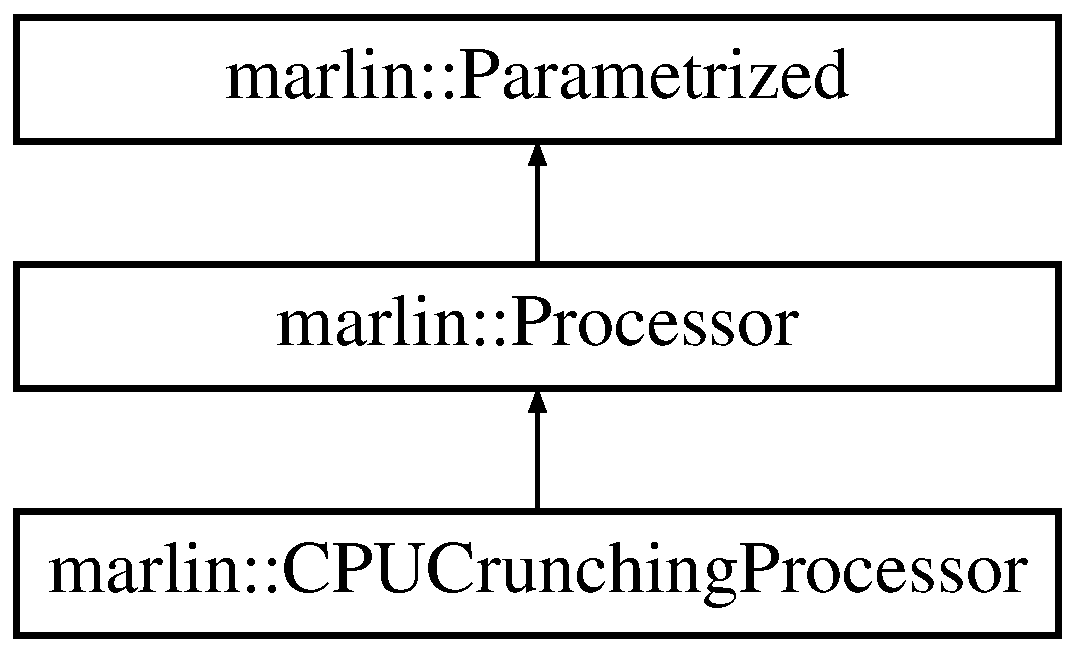
\includegraphics[height=3.000000cm]{classmarlin_1_1CPUCrunchingProcessor}
\end{center}
\end{figure}
\subsection*{Public Member Functions}
\begin{DoxyCompactItemize}
\item 
\mbox{\label{classmarlin_1_1CPUCrunchingProcessor_a5036b337fface30a808b59d55b645f12}} 
\textbf{ Processor} $\ast$ \textbf{ new\+Processor} ()
\begin{DoxyCompactList}\small\item\em Return a new instance of the processor (factory method) \end{DoxyCompactList}\item 
void \textbf{ init} ()
\begin{DoxyCompactList}\small\item\em Initialize the processor. \end{DoxyCompactList}\item 
void \textbf{ process\+Event} (E\+V\+E\+N\+T\+::\+L\+C\+Event $\ast$evt)
\begin{DoxyCompactList}\small\item\em Process an input event. \end{DoxyCompactList}\end{DoxyCompactItemize}
\subsection*{Additional Inherited Members}


\subsection{Detailed Description}
Simple processor crunching C\+PU time for n milliseconds. 

\subparagraph*{Input -\/ Prerequisites}

none \subparagraph*{Output}

none  Crunch\+Time the time in millisecond to crunch C\+PU

\begin{DoxyAuthor}{Author}
R.\+Ete, D\+E\+SY 
\end{DoxyAuthor}


\subsection{Member Function Documentation}
\mbox{\label{classmarlin_1_1CPUCrunchingProcessor_a7b59906fb597c07394f95c3c2dcf978b}} 
\index{marlin\+::\+C\+P\+U\+Crunching\+Processor@{marlin\+::\+C\+P\+U\+Crunching\+Processor}!init@{init}}
\index{init@{init}!marlin\+::\+C\+P\+U\+Crunching\+Processor@{marlin\+::\+C\+P\+U\+Crunching\+Processor}}
\subsubsection{init()}
{\footnotesize\ttfamily void marlin\+::\+C\+P\+U\+Crunching\+Processor\+::init (\begin{DoxyParamCaption}{ }\end{DoxyParamCaption})\hspace{0.3cm}{\ttfamily [virtual]}}



Initialize the processor. 

Called at the begin of the job before anything is read. Use to initialize the processor, e.\+g. book histograms. 

Reimplemented from \textbf{ marlin\+::\+Processor} \doxyref{}{p.}{classmarlin_1_1Processor_a8194fb92a428de40ea9d891c8c8aed6b}.



References marlin\+::\+Processor\+::print\+Parameters(), and marlin\+::\+Processor\+Api\+::register\+For\+Random\+Seeds().



Referenced by new\+Processor().

\mbox{\label{classmarlin_1_1CPUCrunchingProcessor_a72dd012f547e203c22fdfc15396a9281}} 
\index{marlin\+::\+C\+P\+U\+Crunching\+Processor@{marlin\+::\+C\+P\+U\+Crunching\+Processor}!process\+Event@{process\+Event}}
\index{process\+Event@{process\+Event}!marlin\+::\+C\+P\+U\+Crunching\+Processor@{marlin\+::\+C\+P\+U\+Crunching\+Processor}}
\subsubsection{process\+Event()}
{\footnotesize\ttfamily void marlin\+::\+C\+P\+U\+Crunching\+Processor\+::process\+Event (\begin{DoxyParamCaption}\item[{E\+V\+E\+N\+T\+::\+L\+C\+Event $\ast$}]{ }\end{DoxyParamCaption})\hspace{0.3cm}{\ttfamily [virtual]}}



Process an input event. 

Called for every event -\/ the working horse. 

Reimplemented from \textbf{ marlin\+::\+Processor} \doxyref{}{p.}{classmarlin_1_1Processor_a5bee49b5515f59fae755e0a26dfae91a}.



References marlin\+::\+Processor\+Api\+::get\+Random\+Seed().



Referenced by new\+Processor().



The documentation for this class was generated from the following file\+:\begin{DoxyCompactItemize}
\item 
C\+P\+U\+Crunching\+Processor.\+cc\end{DoxyCompactItemize}

\section{marlin\+:\+:Data\+Source\+Plugin Class Reference}
\label{classmarlin_1_1DataSourcePlugin}\index{marlin\+::\+Data\+Source\+Plugin@{marlin\+::\+Data\+Source\+Plugin}}


\doxyref{Data\+Source\+Plugin}{p.}{classmarlin_1_1DataSourcePlugin} class Responsible for reading/getting L\+C\+Event and L\+C\+Run\+Header in the framework for further processing.  




{\ttfamily \#include $<$Data\+Source\+Plugin.\+h$>$}

Inheritance diagram for marlin\+:\+:Data\+Source\+Plugin\+:\begin{figure}[H]
\begin{center}
\leavevmode
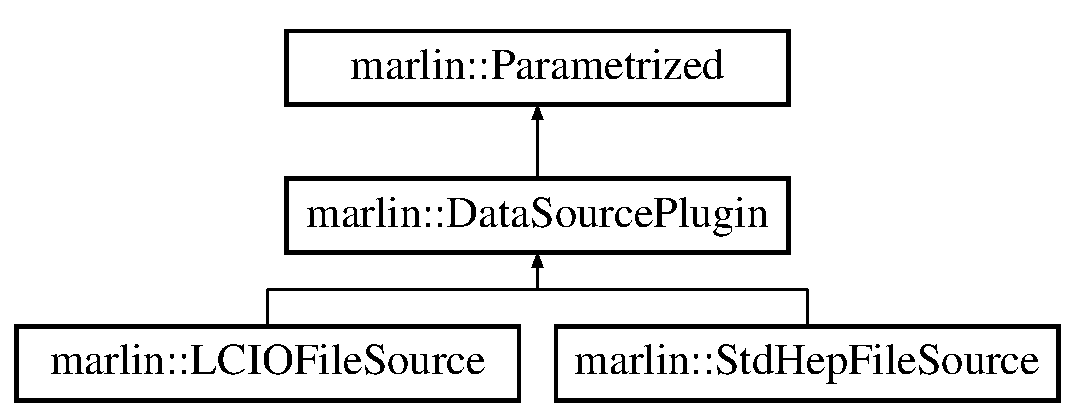
\includegraphics[height=3.000000cm]{classmarlin_1_1DataSourcePlugin}
\end{center}
\end{figure}
\subsection*{Public Types}
\begin{DoxyCompactItemize}
\item 
\mbox{\label{classmarlin_1_1DataSourcePlugin_a9f178249c14e52ed972923d52ba3a4a6}} 
using {\bfseries Event\+Function} = std\+::function$<$ void(std\+::shared\+\_\+ptr$<$ E\+V\+E\+N\+T\+::\+L\+C\+Event $>$)$>$
\item 
\mbox{\label{classmarlin_1_1DataSourcePlugin_ad88f0869d0853c6e2ac8f6293ad36d0d}} 
using {\bfseries Run\+Header\+Function} = std\+::function$<$ void(std\+::shared\+\_\+ptr$<$ E\+V\+E\+N\+T\+::\+L\+C\+Run\+Header $>$)$>$
\item 
\mbox{\label{classmarlin_1_1DataSourcePlugin_a8443fdd38a51d199266e2871a0eed297}} 
using {\bfseries Logger} = Logging\+::\+Logger
\end{DoxyCompactItemize}
\subsection*{Public Member Functions}
\begin{DoxyCompactItemize}
\item 
\textbf{ Data\+Source\+Plugin} (const std\+::string \&dstype)
\begin{DoxyCompactList}\small\item\em Constructor. \end{DoxyCompactList}\item 
void \textbf{ init} (const \textbf{ Application} $\ast$app)
\begin{DoxyCompactList}\small\item\em Initialize the plugin using application parameters. \end{DoxyCompactList}\item 
\mbox{\label{classmarlin_1_1DataSourcePlugin_a765745cfb812360c2bdc423360247adf}} 
const std\+::string \& \textbf{ type} () const
\begin{DoxyCompactList}\small\item\em Get the data source type. \end{DoxyCompactList}\item 
\mbox{\label{classmarlin_1_1DataSourcePlugin_aea2abca77ef499be9651e439f778f300}} 
const std\+::string \& \textbf{ description} () const
\begin{DoxyCompactList}\small\item\em Get the data source description. \end{DoxyCompactList}\item 
\mbox{\label{classmarlin_1_1DataSourcePlugin_ac050d7005038eb8eff12343b3f1c9bd0}} 
virtual void \textbf{ init} ()=0
\begin{DoxyCompactList}\small\item\em Initialize the plugin. \end{DoxyCompactList}\item 
virtual bool \textbf{ read\+One} ()=0
\begin{DoxyCompactList}\small\item\em Read one record from the input stream. \end{DoxyCompactList}\item 
\mbox{\label{classmarlin_1_1DataSourcePlugin_a712a9cb0065c2058e6c6494c015074fc}} 
virtual void \textbf{ read\+All} ()
\begin{DoxyCompactList}\small\item\em Read the full stream until the end See \doxyref{read\+One()}{p.}{classmarlin_1_1DataSourcePlugin_a9e174b63facdc108425e79fca9022404} for details. \end{DoxyCompactList}\item 
void \textbf{ on\+Event\+Read} (Event\+Function func)
\begin{DoxyCompactList}\small\item\em Set the callback function to process on event read. \end{DoxyCompactList}\item 
void \textbf{ on\+Run\+Header\+Read} (Run\+Header\+Function func)
\begin{DoxyCompactList}\small\item\em Set the callback function to process on run header read. \end{DoxyCompactList}\item 
\mbox{\label{classmarlin_1_1DataSourcePlugin_a672029270e97285c09eae4ab80fd6ef8}} 
Logger \textbf{ logger} () const
\begin{DoxyCompactList}\small\item\em Get the plugin logger. \end{DoxyCompactList}\end{DoxyCompactItemize}
\subsection*{Protected Member Functions}
\begin{DoxyCompactItemize}
\item 
void \textbf{ process\+Run\+Header} (std\+::shared\+\_\+ptr$<$ E\+V\+E\+N\+T\+::\+L\+C\+Run\+Header $>$ rhdr)
\begin{DoxyCompactList}\small\item\em Must be called by daughter classes in read\+Stream() to process an event in the framework. \end{DoxyCompactList}\item 
void \textbf{ process\+Event} (std\+::shared\+\_\+ptr$<$ E\+V\+E\+N\+T\+::\+L\+C\+Event $>$ event)
\begin{DoxyCompactList}\small\item\em Must be called by daughter classes in read\+Stream() to process an event in the framework. \end{DoxyCompactList}\end{DoxyCompactItemize}
\subsection*{Protected Attributes}
\begin{DoxyCompactItemize}
\item 
\mbox{\label{classmarlin_1_1DataSourcePlugin_a54050a821803867a90dbb2e7538ebbb3}} 
std\+::string \textbf{ \+\_\+description} \{\char`\"{}No \textbf{ description}\char`\"{}\}
\begin{DoxyCompactList}\small\item\em $<$ The data source description \end{DoxyCompactList}\end{DoxyCompactItemize}


\subsection{Detailed Description}
\doxyref{Data\+Source\+Plugin}{p.}{classmarlin_1_1DataSourcePlugin} class Responsible for reading/getting L\+C\+Event and L\+C\+Run\+Header in the framework for further processing. 

\subsection{Constructor \& Destructor Documentation}
\mbox{\label{classmarlin_1_1DataSourcePlugin_abc28a03b6f994da1673ac2c70acc5cd9}} 
\index{marlin\+::\+Data\+Source\+Plugin@{marlin\+::\+Data\+Source\+Plugin}!Data\+Source\+Plugin@{Data\+Source\+Plugin}}
\index{Data\+Source\+Plugin@{Data\+Source\+Plugin}!marlin\+::\+Data\+Source\+Plugin@{marlin\+::\+Data\+Source\+Plugin}}
\subsubsection{Data\+Source\+Plugin()}
{\footnotesize\ttfamily marlin\+::\+Data\+Source\+Plugin\+::\+Data\+Source\+Plugin (\begin{DoxyParamCaption}\item[{const std\+::string \&}]{dstype }\end{DoxyParamCaption})}



Constructor. 


\begin{DoxyParams}{Parameters}
{\em dstype} & the data source plugin type \\
\hline
\end{DoxyParams}


References marlin\+::\+Logging\+::create\+Logger().



\subsection{Member Function Documentation}
\mbox{\label{classmarlin_1_1DataSourcePlugin_a56cdc244de7fe56c2ab7206c08265336}} 
\index{marlin\+::\+Data\+Source\+Plugin@{marlin\+::\+Data\+Source\+Plugin}!init@{init}}
\index{init@{init}!marlin\+::\+Data\+Source\+Plugin@{marlin\+::\+Data\+Source\+Plugin}}
\subsubsection{init()}
{\footnotesize\ttfamily void marlin\+::\+Data\+Source\+Plugin\+::init (\begin{DoxyParamCaption}\item[{const \textbf{ Application} $\ast$}]{app }\end{DoxyParamCaption})}



Initialize the plugin using application parameters. 


\begin{DoxyParams}{Parameters}
{\em app} & the application in which the plugin is running \\
\hline
\end{DoxyParams}


References marlin\+::\+Application\+::create\+Logger(), marlin\+::\+Application\+::data\+Source\+Parameters(), description(), init(), logger(), marlin\+::\+Parametrized\+::set\+Parameters(), and type().

\mbox{\label{classmarlin_1_1DataSourcePlugin_a1f91ed1135604736ee6bda7d4e303f1e}} 
\index{marlin\+::\+Data\+Source\+Plugin@{marlin\+::\+Data\+Source\+Plugin}!on\+Event\+Read@{on\+Event\+Read}}
\index{on\+Event\+Read@{on\+Event\+Read}!marlin\+::\+Data\+Source\+Plugin@{marlin\+::\+Data\+Source\+Plugin}}
\subsubsection{on\+Event\+Read()}
{\footnotesize\ttfamily void marlin\+::\+Data\+Source\+Plugin\+::on\+Event\+Read (\begin{DoxyParamCaption}\item[{Event\+Function}]{func }\end{DoxyParamCaption})}



Set the callback function to process on event read. 


\begin{DoxyParams}{Parameters}
{\em func} & the callback function \\
\hline
\end{DoxyParams}
\mbox{\label{classmarlin_1_1DataSourcePlugin_afe70af555a35ae259620b8ae1cbf0ccb}} 
\index{marlin\+::\+Data\+Source\+Plugin@{marlin\+::\+Data\+Source\+Plugin}!on\+Run\+Header\+Read@{on\+Run\+Header\+Read}}
\index{on\+Run\+Header\+Read@{on\+Run\+Header\+Read}!marlin\+::\+Data\+Source\+Plugin@{marlin\+::\+Data\+Source\+Plugin}}
\subsubsection{on\+Run\+Header\+Read()}
{\footnotesize\ttfamily void marlin\+::\+Data\+Source\+Plugin\+::on\+Run\+Header\+Read (\begin{DoxyParamCaption}\item[{Run\+Header\+Function}]{func }\end{DoxyParamCaption})}



Set the callback function to process on run header read. 


\begin{DoxyParams}{Parameters}
{\em func} & the callback function \\
\hline
\end{DoxyParams}
\mbox{\label{classmarlin_1_1DataSourcePlugin_add4afa8b047d3a2e4e33a9957e75d9bb}} 
\index{marlin\+::\+Data\+Source\+Plugin@{marlin\+::\+Data\+Source\+Plugin}!process\+Event@{process\+Event}}
\index{process\+Event@{process\+Event}!marlin\+::\+Data\+Source\+Plugin@{marlin\+::\+Data\+Source\+Plugin}}
\subsubsection{process\+Event()}
{\footnotesize\ttfamily void marlin\+::\+Data\+Source\+Plugin\+::process\+Event (\begin{DoxyParamCaption}\item[{std\+::shared\+\_\+ptr$<$ E\+V\+E\+N\+T\+::\+L\+C\+Event $>$}]{event }\end{DoxyParamCaption})\hspace{0.3cm}{\ttfamily [protected]}}



Must be called by daughter classes in read\+Stream() to process an event in the framework. 


\begin{DoxyParams}{Parameters}
{\em event} & the event to process \\
\hline
\end{DoxyParams}
\mbox{\label{classmarlin_1_1DataSourcePlugin_a769e257658ee89c176857191773c26b3}} 
\index{marlin\+::\+Data\+Source\+Plugin@{marlin\+::\+Data\+Source\+Plugin}!process\+Run\+Header@{process\+Run\+Header}}
\index{process\+Run\+Header@{process\+Run\+Header}!marlin\+::\+Data\+Source\+Plugin@{marlin\+::\+Data\+Source\+Plugin}}
\subsubsection{process\+Run\+Header()}
{\footnotesize\ttfamily void marlin\+::\+Data\+Source\+Plugin\+::process\+Run\+Header (\begin{DoxyParamCaption}\item[{std\+::shared\+\_\+ptr$<$ E\+V\+E\+N\+T\+::\+L\+C\+Run\+Header $>$}]{rhdr }\end{DoxyParamCaption})\hspace{0.3cm}{\ttfamily [protected]}}



Must be called by daughter classes in read\+Stream() to process an event in the framework. 


\begin{DoxyParams}{Parameters}
{\em event} & the event to process \\
\hline
\end{DoxyParams}
\mbox{\label{classmarlin_1_1DataSourcePlugin_a9e174b63facdc108425e79fca9022404}} 
\index{marlin\+::\+Data\+Source\+Plugin@{marlin\+::\+Data\+Source\+Plugin}!read\+One@{read\+One}}
\index{read\+One@{read\+One}!marlin\+::\+Data\+Source\+Plugin@{marlin\+::\+Data\+Source\+Plugin}}
\subsubsection{read\+One()}
{\footnotesize\ttfamily virtual bool marlin\+::\+Data\+Source\+Plugin\+::read\+One (\begin{DoxyParamCaption}{ }\end{DoxyParamCaption})\hspace{0.3cm}{\ttfamily [pure virtual]}}



Read one record from the input stream. 

Users must call \doxyref{process\+Run\+Header()}{p.}{classmarlin_1_1DataSourcePlugin_a769e257658ee89c176857191773c26b3} or \doxyref{process\+Event()}{p.}{classmarlin_1_1DataSourcePlugin_add4afa8b047d3a2e4e33a9957e75d9bb} to forward it to the framework. Returns true on success. If the end of the stream is reached, return false. 

Implemented in \textbf{ marlin\+::\+L\+C\+I\+O\+File\+Source} \doxyref{}{p.}{classmarlin_1_1LCIOFileSource_aed4e06595dbb4b22b50766369d0c4809}, and \textbf{ marlin\+::\+Std\+Hep\+File\+Source} \doxyref{}{p.}{classmarlin_1_1StdHepFileSource_a0dc43528a14d38dc6277ba300f5fecb8}.



Referenced by read\+All().



The documentation for this class was generated from the following files\+:\begin{DoxyCompactItemize}
\item 
Data\+Source\+Plugin.\+h\item 
Data\+Source\+Plugin.\+cc\end{DoxyCompactItemize}

\section{marlin\+:\+:D\+D4hep\+Geometry Class Reference}
\label{classmarlin_1_1DD4hepGeometry}\index{marlin\+::\+D\+D4hep\+Geometry@{marlin\+::\+D\+D4hep\+Geometry}}


\doxyref{D\+D4hep\+Geometry}{p.}{classmarlin_1_1DD4hepGeometry} class Responsible for loading D\+D4hep geometry in Marlin.  


Inheritance diagram for marlin\+:\+:D\+D4hep\+Geometry\+:\begin{figure}[H]
\begin{center}
\leavevmode
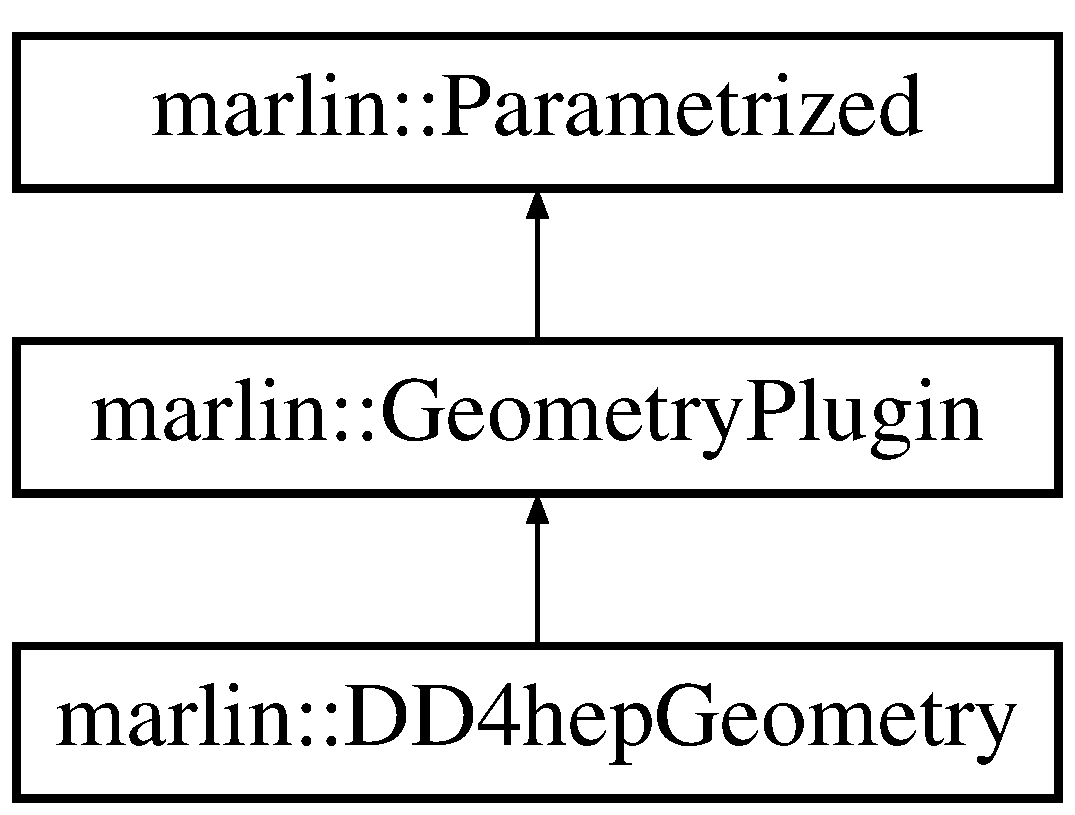
\includegraphics[height=3.000000cm]{classmarlin_1_1DD4hepGeometry}
\end{center}
\end{figure}
\subsection*{Public Member Functions}
\begin{DoxyCompactItemize}
\item 
\mbox{\label{classmarlin_1_1DD4hepGeometry_a1755feccb117ee6d3c67a9ea9912dafa}} 
{\bfseries D\+D4hep\+Geometry} (const \textbf{ D\+D4hep\+Geometry} \&)=delete
\item 
\mbox{\label{classmarlin_1_1DD4hepGeometry_a3498a11384b5c1c0a75883e25019a219}} 
\textbf{ D\+D4hep\+Geometry} \& {\bfseries operator=} (const \textbf{ D\+D4hep\+Geometry} \&)=delete
\end{DoxyCompactItemize}
\subsection*{Protected Member Functions}
\begin{DoxyCompactItemize}
\item 
\mbox{\label{classmarlin_1_1DD4hepGeometry_aec15c25385f26ded6f9b5f0ad2e83760}} 
void \textbf{ load\+Geometry} ()
\begin{DoxyCompactList}\small\item\em Load the geometry. \end{DoxyCompactList}\item 
\mbox{\label{classmarlin_1_1DD4hepGeometry_a89b358871e58b71402537949edb83c99}} 
const void $\ast$ \textbf{ handle} () const
\begin{DoxyCompactList}\small\item\em Get a handle on the geometry instance. \end{DoxyCompactList}\item 
\mbox{\label{classmarlin_1_1DD4hepGeometry_a8e71c18209d78b489f3c46bf859f4a10}} 
void \textbf{ destroy} ()
\begin{DoxyCompactList}\small\item\em Cleanup geometry. \end{DoxyCompactList}\item 
\mbox{\label{classmarlin_1_1DD4hepGeometry_af8a8d26d7f5bb7e6a1b1053870aac62f}} 
std\+::type\+\_\+index \textbf{ type\+Index} () const
\begin{DoxyCompactList}\small\item\em Get a type index object from the geometry handle. \end{DoxyCompactList}\item 
\mbox{\label{classmarlin_1_1DD4hepGeometry_af916f5554c4c01c30fb6353f9b324c5a}} 
void \textbf{ dump\+Geometry} () const
\begin{DoxyCompactList}\small\item\em Dump the geometry in the console. \end{DoxyCompactList}\end{DoxyCompactItemize}
\subsection*{Additional Inherited Members}


\subsection{Detailed Description}
\doxyref{D\+D4hep\+Geometry}{p.}{classmarlin_1_1DD4hepGeometry} class Responsible for loading D\+D4hep geometry in Marlin. 

The documentation for this class was generated from the following file\+:\begin{DoxyCompactItemize}
\item 
D\+D4hep\+Geometry.\+cc\end{DoxyCompactItemize}

\section{marlin\+:\+:Empty\+Geometry Class Reference}
\label{classmarlin_1_1EmptyGeometry}\index{marlin\+::\+Empty\+Geometry@{marlin\+::\+Empty\+Geometry}}


\doxyref{Empty\+Geometry}{p.}{classmarlin_1_1EmptyGeometry} class Implement an empty geometry.  


Inheritance diagram for marlin\+:\+:Empty\+Geometry\+:\begin{figure}[H]
\begin{center}
\leavevmode
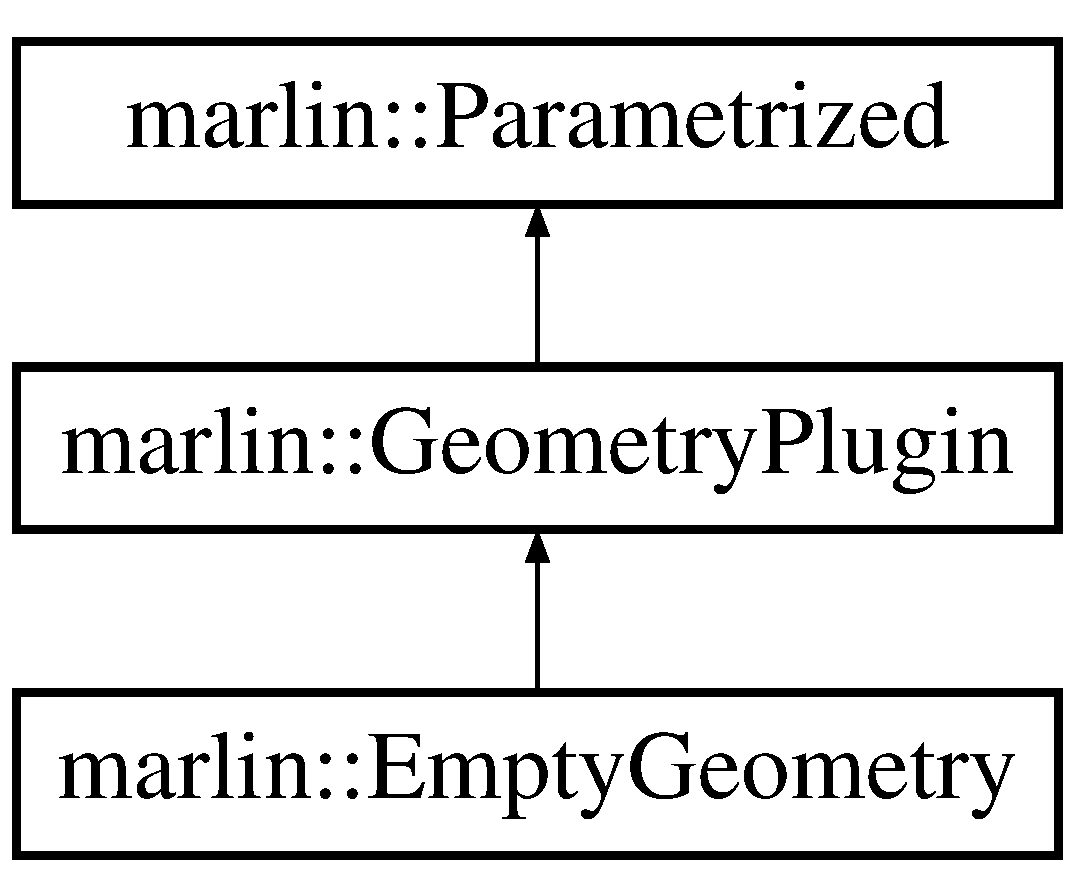
\includegraphics[height=3.000000cm]{classmarlin_1_1EmptyGeometry}
\end{center}
\end{figure}
\subsection*{Public Member Functions}
\begin{DoxyCompactItemize}
\item 
\mbox{\label{classmarlin_1_1EmptyGeometry_a9e4e6720abc9fd3ba70558d6b61f2d53}} 
{\bfseries Empty\+Geometry} (const \textbf{ Empty\+Geometry} \&)=delete
\item 
\mbox{\label{classmarlin_1_1EmptyGeometry_ad97f987a7b634fefa9516aa14edd1717}} 
\textbf{ Empty\+Geometry} \& {\bfseries operator=} (const \textbf{ Empty\+Geometry} \&)=delete
\end{DoxyCompactItemize}
\subsection*{Protected Member Functions}
\begin{DoxyCompactItemize}
\item 
\mbox{\label{classmarlin_1_1EmptyGeometry_ad6f1d16609ebfbdcb690920d7f472ba4}} 
void \textbf{ load\+Geometry} ()
\begin{DoxyCompactList}\small\item\em Load the geometry. \end{DoxyCompactList}\item 
\mbox{\label{classmarlin_1_1EmptyGeometry_acd1c038e2465e8c3292304467e012e21}} 
const void $\ast$ \textbf{ handle} () const
\begin{DoxyCompactList}\small\item\em Get a handle on the geometry instance. \end{DoxyCompactList}\item 
\mbox{\label{classmarlin_1_1EmptyGeometry_ad6c3301662952dd0ef2f81619a620b0d}} 
void \textbf{ destroy} ()
\begin{DoxyCompactList}\small\item\em Cleanup geometry. \end{DoxyCompactList}\item 
\mbox{\label{classmarlin_1_1EmptyGeometry_a1d53939e369faa1db4240ad4d15108d1}} 
std\+::type\+\_\+index \textbf{ type\+Index} () const
\begin{DoxyCompactList}\small\item\em Get a type index object from the geometry handle. \end{DoxyCompactList}\item 
\mbox{\label{classmarlin_1_1EmptyGeometry_a95cd9a0fd9416f5a946915d7fc2974e6}} 
void \textbf{ dump\+Geometry} () const
\begin{DoxyCompactList}\small\item\em Dump the geometry in the console. \end{DoxyCompactList}\end{DoxyCompactItemize}
\subsection*{Additional Inherited Members}


\subsection{Detailed Description}
\doxyref{Empty\+Geometry}{p.}{classmarlin_1_1EmptyGeometry} class Implement an empty geometry. 

The documentation for this class was generated from the following file\+:\begin{DoxyCompactItemize}
\item 
Geometry\+Plugin.\+cc\end{DoxyCompactItemize}

\section{marlin\+:\+:Error\+Of\+Sigma Class Reference}
\label{classmarlin_1_1ErrorOfSigma}\index{marlin\+::\+Error\+Of\+Sigma@{marlin\+::\+Error\+Of\+Sigma}}


Small helper class that computes the lower and upper error of sigma assuming a normal distribution, i.\+e.  




{\ttfamily \#include $<$Error\+Of\+Sigma.\+h$>$}

\subsection*{Public Member Functions}
\begin{DoxyCompactItemize}
\item 
\mbox{\label{classmarlin_1_1ErrorOfSigma_ae7b41d5337dabefc0630ef1c825e43d8}} 
\textbf{ Error\+Of\+Sigma} (unsigned n)
\begin{DoxyCompactList}\small\item\em C\textquotesingle{}tor takes the number of measured values. \end{DoxyCompactList}\item 
virtual \textbf{ $\sim$\+Error\+Of\+Sigma} ()
\begin{DoxyCompactList}\small\item\em Virtual d\textquotesingle{}tor. \end{DoxyCompactList}\item 
\mbox{\label{classmarlin_1_1ErrorOfSigma_a5eea304e56dbf80281b418a8946c2097}} 
double \textbf{ lower\+Error} (double sigma)
\begin{DoxyCompactList}\small\item\em The lower error of sigma. \end{DoxyCompactList}\item 
\mbox{\label{classmarlin_1_1ErrorOfSigma_afeaa57f2c02cb68a66b0f6aeaa23d4d5}} 
double \textbf{ upper\+Error} (double sigma)
\begin{DoxyCompactList}\small\item\em The upper error of sigma. \end{DoxyCompactList}\end{DoxyCompactItemize}
\subsection*{Protected Member Functions}
\begin{DoxyCompactItemize}
\item 
\mbox{\label{classmarlin_1_1ErrorOfSigma_af336af4a84c4e860367f1aa760164054}} 
virtual double \textbf{ get\+Chi\+Squared\+Plus} ()
\begin{DoxyCompactList}\small\item\em Returns the chisquared value with P(chisquared) == 0.\+84. \end{DoxyCompactList}\item 
\mbox{\label{classmarlin_1_1ErrorOfSigma_a14ed1cbadcd749d504529ee45625a5e6}} 
virtual double \textbf{ get\+Chi\+Squared\+Minus} ()
\begin{DoxyCompactList}\small\item\em Returns the chisquared value with P(chisquared) == 0.\+16. \end{DoxyCompactList}\end{DoxyCompactItemize}
\subsection*{Protected Attributes}
\begin{DoxyCompactItemize}
\item 
\mbox{\label{classmarlin_1_1ErrorOfSigma_ab63edd7ef4330b37ec320bab497c1370}} 
unsigned \textbf{ \+\_\+n}
\begin{DoxyCompactList}\small\item\em The number of degrees of freedom. \end{DoxyCompactList}\end{DoxyCompactItemize}


\subsection{Detailed Description}
Small helper class that computes the lower and upper error of sigma assuming a normal distribution, i.\+e. 

sigma has been computed as sigma = 1. / (n-\/1) $\ast$ S\+U\+M\+\_\+i\+\_\+n( x\+\_\+i -\/ a\+\_\+i )$\ast$$\ast$2.

\begin{DoxyAuthor}{Author}
F. Gaede, D\+E\+SY 
\end{DoxyAuthor}
\begin{DoxyVersion}{Version}

\end{DoxyVersion}
\begin{DoxyParagraph}{Id}
\doxyref{Error\+Of\+Sigma.\+h}{p.}{ErrorOfSigma_8h_source},v 1.\+2 2005-\/10-\/11 12\+:56\+:28 gaede Exp 
\end{DoxyParagraph}


\subsection{Constructor \& Destructor Documentation}
\mbox{\label{classmarlin_1_1ErrorOfSigma_a481541db40c7036c9a11f9b30a195172}} 
\index{marlin\+::\+Error\+Of\+Sigma@{marlin\+::\+Error\+Of\+Sigma}!````~Error\+Of\+Sigma@{$\sim$\+Error\+Of\+Sigma}}
\index{````~Error\+Of\+Sigma@{$\sim$\+Error\+Of\+Sigma}!marlin\+::\+Error\+Of\+Sigma@{marlin\+::\+Error\+Of\+Sigma}}
\subsubsection{$\sim$\+Error\+Of\+Sigma()}
{\footnotesize\ttfamily virtual marlin\+::\+Error\+Of\+Sigma\+::$\sim$\+Error\+Of\+Sigma (\begin{DoxyParamCaption}{ }\end{DoxyParamCaption})\hspace{0.3cm}{\ttfamily [inline]}, {\ttfamily [virtual]}}



Virtual d\textquotesingle{}tor. 



References get\+Chi\+Squared\+Minus(), get\+Chi\+Squared\+Plus(), lower\+Error(), and upper\+Error().



The documentation for this class was generated from the following files\+:\begin{DoxyCompactItemize}
\item 
Error\+Of\+Sigma.\+h\item 
Error\+Of\+Sigma.\+cc\end{DoxyCompactItemize}

\section{marlin\+:\+:Event\+Modifier Class Reference}
\label{classmarlin_1_1EventModifier}\index{marlin\+::\+Event\+Modifier@{marlin\+::\+Event\+Modifier}}


Tagging interface for processors that modify the L\+C\+IO event.  




{\ttfamily \#include $<$Event\+Modifier.\+h$>$}

Inheritance diagram for marlin\+:\+:Event\+Modifier\+:\begin{figure}[H]
\begin{center}
\leavevmode
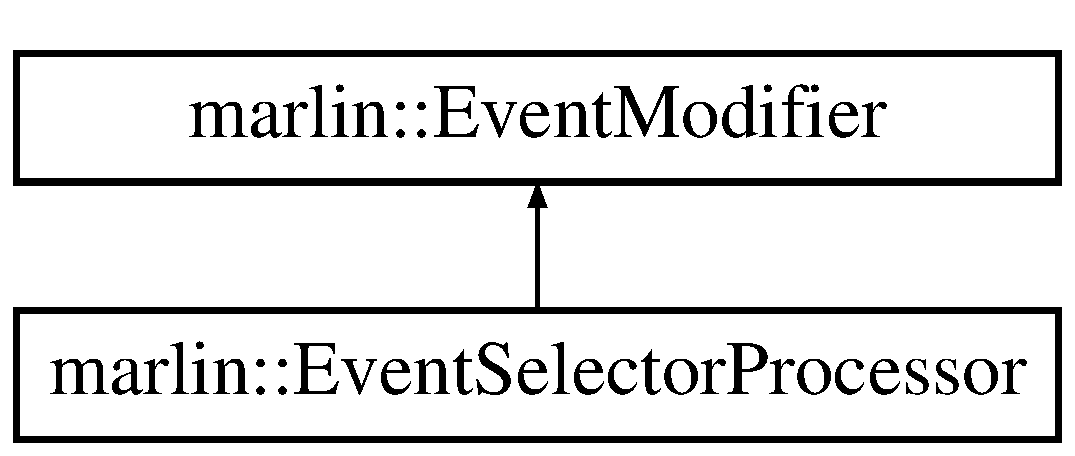
\includegraphics[height=2.000000cm]{classmarlin_1_1EventModifier}
\end{center}
\end{figure}
\subsection*{Public Member Functions}
\begin{DoxyCompactItemize}
\item 
\mbox{\label{classmarlin_1_1EventModifier_a839dc570df2ed072b56bcd3c12d396b1}} 
virtual void \textbf{ modify\+Event} (E\+V\+E\+N\+T\+::\+L\+C\+Event $\ast$)=0
\begin{DoxyCompactList}\small\item\em Implement to modify the event. \end{DoxyCompactList}\item 
\mbox{\label{classmarlin_1_1EventModifier_a87ed425ee54f74893efd0f2ee3244d2a}} 
virtual void \textbf{ modify\+Run\+Header} (E\+V\+E\+N\+T\+::\+L\+C\+Run\+Header $\ast$)
\begin{DoxyCompactList}\small\item\em Implement to modify the run header. \end{DoxyCompactList}\item 
\mbox{\label{classmarlin_1_1EventModifier_a9eecc7d95199af33e9b2228140b97b27}} 
virtual const std\+::string \& \textbf{ name} () const =0
\begin{DoxyCompactList}\small\item\em Return name of this event modifier. \end{DoxyCompactList}\item 
\mbox{\label{classmarlin_1_1EventModifier_aa5a2afc611df6dfbd238d95ea20e0976}} 
virtual \textbf{ $\sim$\+Event\+Modifier} ()
\begin{DoxyCompactList}\small\item\em Return name of log level name this event modifier. \end{DoxyCompactList}\end{DoxyCompactItemize}


\subsection{Detailed Description}
Tagging interface for processors that modify the L\+C\+IO event. 

\begin{DoxyAuthor}{Author}
F. Gaede, D\+E\+SY 
\end{DoxyAuthor}
\begin{DoxyVersion}{Version}

\end{DoxyVersion}
\begin{DoxyParagraph}{Id}
\doxyref{Event\+Modifier.\+h}{p.}{EventModifier_8h_source},v 1.\+2 2007-\/08-\/17 11\+:21\+:55 gaede Exp 
\end{DoxyParagraph}


The documentation for this class was generated from the following file\+:\begin{DoxyCompactItemize}
\item 
Event\+Modifier.\+h\end{DoxyCompactItemize}

\section{marlin\+:\+:Event\+Selector\+Processor Class Reference}
\label{classmarlin_1_1EventSelectorProcessor}\index{marlin\+::\+Event\+Selector\+Processor@{marlin\+::\+Event\+Selector\+Processor}}


Simple event selector processor.  


Inheritance diagram for marlin\+:\+:Event\+Selector\+Processor\+:\begin{figure}[H]
\begin{center}
\leavevmode
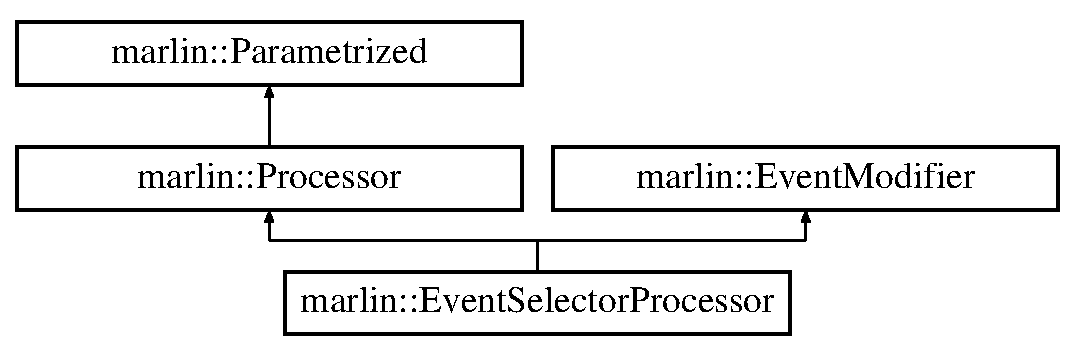
\includegraphics[height=3.000000cm]{classmarlin_1_1EventSelectorProcessor}
\end{center}
\end{figure}
\subsection*{Public Member Functions}
\begin{DoxyCompactItemize}
\item 
\mbox{\label{classmarlin_1_1EventSelectorProcessor_a9f595ab4d3f6c380d0ecda08244747d5}} 
\textbf{ Event\+Selector\+Processor} ()
\begin{DoxyCompactList}\small\item\em Constructor. \end{DoxyCompactList}\item 
\mbox{\label{classmarlin_1_1EventSelectorProcessor_a14b8aeccbe2e3eb438c720bff7bd75e7}} 
\textbf{ Processor} $\ast$ \textbf{ new\+Processor} ()
\begin{DoxyCompactList}\small\item\em Return a new instance of the processor (factory method) \end{DoxyCompactList}\item 
void \textbf{ init} ()
\begin{DoxyCompactList}\small\item\em Initialize the processor. \end{DoxyCompactList}\item 
void \textbf{ process\+Event} (E\+V\+E\+N\+T\+::\+L\+C\+Event $\ast$evt)
\begin{DoxyCompactList}\small\item\em Process an input event. \end{DoxyCompactList}\item 
\mbox{\label{classmarlin_1_1EventSelectorProcessor_a5bd533aee70661acc2d5f0f18f588274}} 
const std\+::string \& \textbf{ name} () const
\begin{DoxyCompactList}\small\item\em Return name of this event modifier. \end{DoxyCompactList}\item 
\mbox{\label{classmarlin_1_1EventSelectorProcessor_a7363bd1e06a76e3ae4e63b0e968babcd}} 
void \textbf{ modify\+Event} (E\+V\+E\+N\+T\+::\+L\+C\+Event $\ast$evt)
\begin{DoxyCompactList}\small\item\em Implement to modify the event. \end{DoxyCompactList}\end{DoxyCompactItemize}
\subsection*{Protected Attributes}
\begin{DoxyCompactItemize}
\item 
E\+V\+E\+N\+T\+::\+Int\+Vec \textbf{ \+\_\+evt\+List} \{\}
\begin{DoxyCompactList}\small\item\em $<$ The event list parameter (list of \char`\"{}run event\char`\"{} ids) \end{DoxyCompactList}\item 
\mbox{\label{classmarlin_1_1EventSelectorProcessor_a120860639677474c7e4b1253c666b3d8}} 
Event\+Number\+Set {\bfseries \+\_\+evt\+Set} \{\}
\end{DoxyCompactItemize}
\subsection*{Additional Inherited Members}


\subsection{Detailed Description}
Simple event selector processor. 

Returns true if the given event was specified in the Even\+List parameter.

\subparagraph*{Output}

returns true or false


\begin{DoxyParams}{Parameters}
{\em Event\+List} & pairs of\+: Event\+Number Run\+Number\\
\hline
\end{DoxyParams}
\begin{DoxyAuthor}{Author}
F. Gaede, D\+E\+SY 
\end{DoxyAuthor}
\begin{DoxyVersion}{Version}
\$\+Id\+:\$ 
\end{DoxyVersion}


\subsection{Member Function Documentation}
\mbox{\label{classmarlin_1_1EventSelectorProcessor_aeb4c233b4075fc99c5f146c21ec96d78}} 
\index{marlin\+::\+Event\+Selector\+Processor@{marlin\+::\+Event\+Selector\+Processor}!init@{init}}
\index{init@{init}!marlin\+::\+Event\+Selector\+Processor@{marlin\+::\+Event\+Selector\+Processor}}
\subsubsection{init()}
{\footnotesize\ttfamily void marlin\+::\+Event\+Selector\+Processor\+::init (\begin{DoxyParamCaption}{ }\end{DoxyParamCaption})\hspace{0.3cm}{\ttfamily [virtual]}}



Initialize the processor. 

Called at the begin of the job before anything is read. Use to initialize the processor, e.\+g. book histograms. 

Reimplemented from \textbf{ marlin\+::\+Processor} \doxyref{}{p.}{classmarlin_1_1Processor_a8194fb92a428de40ea9d891c8c8aed6b}.



References \+\_\+evt\+List, and marlin\+::\+Processor\+::print\+Parameters().

\mbox{\label{classmarlin_1_1EventSelectorProcessor_a4f669851b0ccecc53c65e0f589881d66}} 
\index{marlin\+::\+Event\+Selector\+Processor@{marlin\+::\+Event\+Selector\+Processor}!process\+Event@{process\+Event}}
\index{process\+Event@{process\+Event}!marlin\+::\+Event\+Selector\+Processor@{marlin\+::\+Event\+Selector\+Processor}}
\subsubsection{process\+Event()}
{\footnotesize\ttfamily void marlin\+::\+Event\+Selector\+Processor\+::process\+Event (\begin{DoxyParamCaption}\item[{E\+V\+E\+N\+T\+::\+L\+C\+Event $\ast$}]{ }\end{DoxyParamCaption})\hspace{0.3cm}{\ttfamily [virtual]}}



Process an input event. 

Called for every event -\/ the working horse. 

Reimplemented from \textbf{ marlin\+::\+Processor} \doxyref{}{p.}{classmarlin_1_1Processor_a5bee49b5515f59fae755e0a26dfae91a}.



References \+\_\+evt\+List.



Referenced by modify\+Event().



\subsection{Member Data Documentation}
\mbox{\label{classmarlin_1_1EventSelectorProcessor_a4f44b84857e78e0d318eb7e62edd4cf9}} 
\index{marlin\+::\+Event\+Selector\+Processor@{marlin\+::\+Event\+Selector\+Processor}!\+\_\+evt\+List@{\+\_\+evt\+List}}
\index{\+\_\+evt\+List@{\+\_\+evt\+List}!marlin\+::\+Event\+Selector\+Processor@{marlin\+::\+Event\+Selector\+Processor}}
\subsubsection{\+\_\+evt\+List}
{\footnotesize\ttfamily E\+V\+E\+N\+T\+::\+Int\+Vec marlin\+::\+Event\+Selector\+Processor\+::\+\_\+evt\+List \{\}\hspace{0.3cm}{\ttfamily [protected]}}



$<$ The event list parameter (list of \char`\"{}run event\char`\"{} ids) 

The event list as a set 

Referenced by Event\+Selector\+Processor(), init(), and process\+Event().



The documentation for this class was generated from the following file\+:\begin{DoxyCompactItemize}
\item 
Event\+Selector\+Processor.\+cc\end{DoxyCompactItemize}

\section{marlin\+:\+:Expression Struct Reference}
\label{structmarlin_1_1Expression}\index{marlin\+::\+Expression@{marlin\+::\+Expression}}


Helper struct for Logical\+Expression.  




{\ttfamily \#include $<$Logical\+Expressions.\+h$>$}

\subsection*{Public Types}
\begin{DoxyCompactItemize}
\item 
\mbox{\label{structmarlin_1_1Expression_addf45faa237dcfc40f065e4d28873e40}} 
enum {\bfseries Operator} \{ {\bfseries OR}, 
{\bfseries A\+ND}
 \}
\end{DoxyCompactItemize}
\subsection*{Public Attributes}
\begin{DoxyCompactItemize}
\item 
\mbox{\label{structmarlin_1_1Expression_aeab4d1202f39cb6f1600385dae92105f}} 
Operator {\bfseries Operation}
\item 
\mbox{\label{structmarlin_1_1Expression_a050ad00f9ecffbd4d51710eda1806a7e}} 
bool {\bfseries is\+Not}
\item 
\mbox{\label{structmarlin_1_1Expression_a80f37908cb8450e337b50d49925608e4}} 
std\+::string {\bfseries Value}
\end{DoxyCompactItemize}


\subsection{Detailed Description}
Helper struct for Logical\+Expression. 

\begin{DoxyAuthor}{Author}
F. Gaede, D\+E\+SY 
\end{DoxyAuthor}
\begin{DoxyVersion}{Version}

\end{DoxyVersion}
\begin{DoxyParagraph}{Id}
\doxyref{Logical\+Expressions.\+h}{p.}{LogicalExpressions_8h_source},v 1.\+3 2005-\/10-\/11 12\+:56\+:28 gaede Exp 
\end{DoxyParagraph}


The documentation for this struct was generated from the following file\+:\begin{DoxyCompactItemize}
\item 
Logical\+Expressions.\+h\end{DoxyCompactItemize}

\section{marlin\+:\+:Gear\+Geometry Class Reference}
\label{classmarlin_1_1GearGeometry}\index{marlin\+::\+Gear\+Geometry@{marlin\+::\+Gear\+Geometry}}


\doxyref{Gear\+Geometry}{p.}{classmarlin_1_1GearGeometry} class Responsible for loading Gear geometry in Marlin.  


Inheritance diagram for marlin\+:\+:Gear\+Geometry\+:\begin{figure}[H]
\begin{center}
\leavevmode
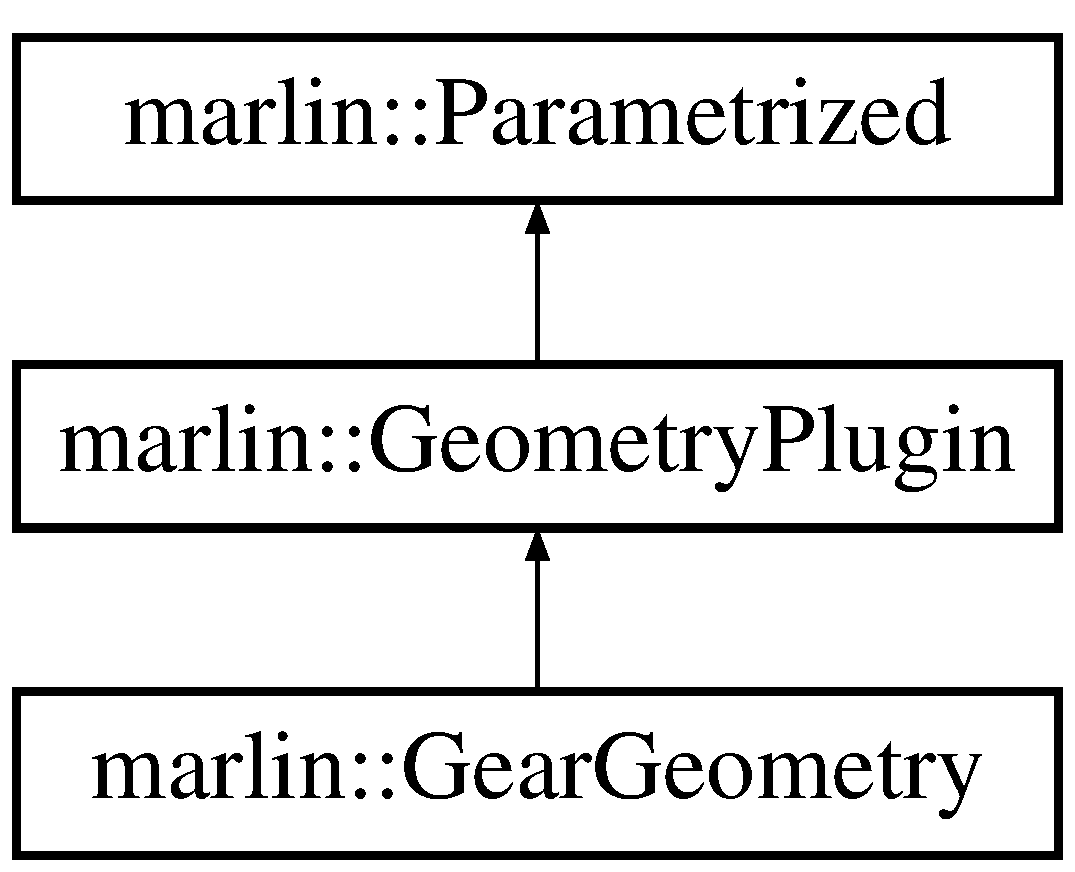
\includegraphics[height=3.000000cm]{classmarlin_1_1GearGeometry}
\end{center}
\end{figure}
\subsection*{Public Member Functions}
\begin{DoxyCompactItemize}
\item 
\mbox{\label{classmarlin_1_1GearGeometry_a7e949c89260c7f7bf9e94b33daf12c94}} 
{\bfseries Gear\+Geometry} (const \textbf{ Gear\+Geometry} \&)=delete
\item 
\mbox{\label{classmarlin_1_1GearGeometry_a059ea4c6cb81973adf5f99a7c2b6e681}} 
\textbf{ Gear\+Geometry} \& {\bfseries operator=} (const \textbf{ Gear\+Geometry} \&)=delete
\end{DoxyCompactItemize}
\subsection*{Protected Member Functions}
\begin{DoxyCompactItemize}
\item 
\mbox{\label{classmarlin_1_1GearGeometry_ad52be8a0f5793610e0bf0d1393617cfa}} 
void \textbf{ load\+Geometry} ()
\begin{DoxyCompactList}\small\item\em Load the geometry. \end{DoxyCompactList}\item 
\mbox{\label{classmarlin_1_1GearGeometry_aa0391e982800797af9ccf7783be4f917}} 
const void $\ast$ \textbf{ handle} () const
\begin{DoxyCompactList}\small\item\em Get a handle on the geometry instance. \end{DoxyCompactList}\item 
\mbox{\label{classmarlin_1_1GearGeometry_a5feddad6772a660056e44d81ee03be3c}} 
void \textbf{ destroy} ()
\begin{DoxyCompactList}\small\item\em Cleanup geometry. \end{DoxyCompactList}\item 
\mbox{\label{classmarlin_1_1GearGeometry_acb37053328a15d72b9002b3999dadd99}} 
std\+::type\+\_\+index \textbf{ type\+Index} () const
\begin{DoxyCompactList}\small\item\em Get a type index object from the geometry handle. \end{DoxyCompactList}\item 
\mbox{\label{classmarlin_1_1GearGeometry_ac36dd250e896792bfa1210cc8185a748}} 
void \textbf{ dump\+Geometry} () const
\begin{DoxyCompactList}\small\item\em Dump the geometry in the console. \end{DoxyCompactList}\end{DoxyCompactItemize}
\subsection*{Additional Inherited Members}


\subsection{Detailed Description}
\doxyref{Gear\+Geometry}{p.}{classmarlin_1_1GearGeometry} class Responsible for loading Gear geometry in Marlin. 

The documentation for this class was generated from the following file\+:\begin{DoxyCompactItemize}
\item 
Gear\+Geometry.\+cc\end{DoxyCompactItemize}

\section{marlin\+:\+:Geometry\+Manager Class Reference}
\label{classmarlin_1_1GeometryManager}\index{marlin\+::\+Geometry\+Manager@{marlin\+::\+Geometry\+Manager}}


\doxyref{Geometry\+Manager}{p.}{classmarlin_1_1GeometryManager} class.  




{\ttfamily \#include $<$Geometry\+Manager.\+h$>$}

\subsection*{Public Types}
\begin{DoxyCompactItemize}
\item 
\mbox{\label{classmarlin_1_1GeometryManager_a807e36fb23ea8f72a87e7bac28afda04}} 
using {\bfseries Logger} = Logging\+::\+Logger
\end{DoxyCompactItemize}
\subsection*{Public Member Functions}
\begin{DoxyCompactItemize}
\item 
\mbox{\label{classmarlin_1_1GeometryManager_a13b43f563d9520fef922664ecefd6a5e}} 
{\bfseries Geometry\+Manager} (const \textbf{ Geometry\+Manager} \&)=delete
\item 
\mbox{\label{classmarlin_1_1GeometryManager_ab7691a6717d5c854ded5b6cc3b31cda5}} 
\textbf{ Geometry\+Manager} \& {\bfseries operator=} (const \textbf{ Geometry\+Manager} \&)=delete
\item 
\mbox{\label{classmarlin_1_1GeometryManager_ac763e57cba29706f027c4f9964660ba6}} 
\textbf{ Geometry\+Manager} ()
\begin{DoxyCompactList}\small\item\em Default constructor. \end{DoxyCompactList}\item 
void \textbf{ init} (const \textbf{ Application} $\ast$\textbf{ app})
\begin{DoxyCompactList}\small\item\em Initialize the geometry manager. \end{DoxyCompactList}\item 
{\footnotesize template$<$typename T $>$ }\\const T $\ast$ \textbf{ geometry} () const
\begin{DoxyCompactList}\small\item\em Get the underlying geometry handle Example\+: \end{DoxyCompactList}\item 
\mbox{\label{classmarlin_1_1GeometryManager_ace34efe0ef2d8aeff33a51444e89599f}} 
std\+::type\+\_\+index \textbf{ type\+Index} () const
\begin{DoxyCompactList}\small\item\em Get the underlying geometry type info. \end{DoxyCompactList}\item 
\mbox{\label{classmarlin_1_1GeometryManager_a3ce06d1eae5637dd82026348e4b0da4b}} 
void \textbf{ clear} ()
\begin{DoxyCompactList}\small\item\em Clear the geometry content. \end{DoxyCompactList}\item 
\mbox{\label{classmarlin_1_1GeometryManager_a248cc35ec62b4ee2de6deee5f7845bea}} 
bool \textbf{ is\+Initialized} () const
\begin{DoxyCompactList}\small\item\em Whether the geometry has been initialized. \end{DoxyCompactList}\item 
\mbox{\label{classmarlin_1_1GeometryManager_aebaf3709c7d06c51a70aa742682d4268}} 
const \textbf{ Application} \& \textbf{ app} () const
\begin{DoxyCompactList}\small\item\em Get the application in which the manager is running Valid only after initialization. \end{DoxyCompactList}\end{DoxyCompactItemize}


\subsection{Detailed Description}
\doxyref{Geometry\+Manager}{p.}{classmarlin_1_1GeometryManager} class. 

Handle a user plugin in charge of loading the geometry in the framework and providing access to it. 

\subsection{Member Function Documentation}
\mbox{\label{classmarlin_1_1GeometryManager_a4257ccc9849a8077c559054aa60fd2ef}} 
\index{marlin\+::\+Geometry\+Manager@{marlin\+::\+Geometry\+Manager}!geometry@{geometry}}
\index{geometry@{geometry}!marlin\+::\+Geometry\+Manager@{marlin\+::\+Geometry\+Manager}}
\subsubsection{geometry()}
{\footnotesize\ttfamily template$<$typename T $>$ \\
const T $\ast$ marlin\+::\+Geometry\+Manager\+::geometry (\begin{DoxyParamCaption}{ }\end{DoxyParamCaption}) const\hspace{0.3cm}{\ttfamily [inline]}}



Get the underlying geometry handle Example\+: 


\begin{DoxyCode}
\textcolor{comment}{// assume Gear geometry has been loaded}
\textcolor{keyword}{const} gear::GearMgr* gearGeo = mgr->geometry<gear::GearMgr>() ;
\textcolor{comment}{// assume DD4hep geometry has been loaded}
\textcolor{keyword}{const} dd4hep::Detector* dd4hepGeo = mgr->geometry<dd4hep::Detector>() ;
\end{DoxyCode}
 

Referenced by marlin\+::\+Processor\+Api\+::gear\+Detector(), and marlin\+::\+Processor\+Api\+::is\+First\+Event().

\mbox{\label{classmarlin_1_1GeometryManager_ab2afa2543af80f642bdbe3f11e96607a}} 
\index{marlin\+::\+Geometry\+Manager@{marlin\+::\+Geometry\+Manager}!init@{init}}
\index{init@{init}!marlin\+::\+Geometry\+Manager@{marlin\+::\+Geometry\+Manager}}
\subsubsection{init()}
{\footnotesize\ttfamily void marlin\+::\+Geometry\+Manager\+::init (\begin{DoxyParamCaption}\item[{const \textbf{ Application} $\ast$}]{app }\end{DoxyParamCaption})}



Initialize the geometry manager. 

Load the geometry plugin service and create the geometry


\begin{DoxyParams}{Parameters}
{\em app} & the application from which to get settings \\
\hline
\end{DoxyParams}


References app(), marlin\+::\+Application\+::create\+Logger(), marlin\+::\+Application\+::geometry\+Parameters(), marlin\+::\+Plugin\+Manager\+::instance(), and is\+Initialized().



The documentation for this class was generated from the following files\+:\begin{DoxyCompactItemize}
\item 
Geometry\+Manager.\+h\item 
Geometry\+Manager.\+cc\end{DoxyCompactItemize}

\section{marlin\+:\+:Geometry\+Plugin Class Reference}
\label{classmarlin_1_1GeometryPlugin}\index{marlin\+::\+Geometry\+Plugin@{marlin\+::\+Geometry\+Plugin}}


\doxyref{Geometry\+Plugin}{p.}{classmarlin_1_1GeometryPlugin} class Responsible for loading geometry in Marlin and providing access to it through the \doxyref{Geometry\+Manager}{p.}{classmarlin_1_1GeometryManager}.  




{\ttfamily \#include $<$Geometry\+Plugin.\+h$>$}

Inheritance diagram for marlin\+:\+:Geometry\+Plugin\+:\begin{figure}[H]
\begin{center}
\leavevmode
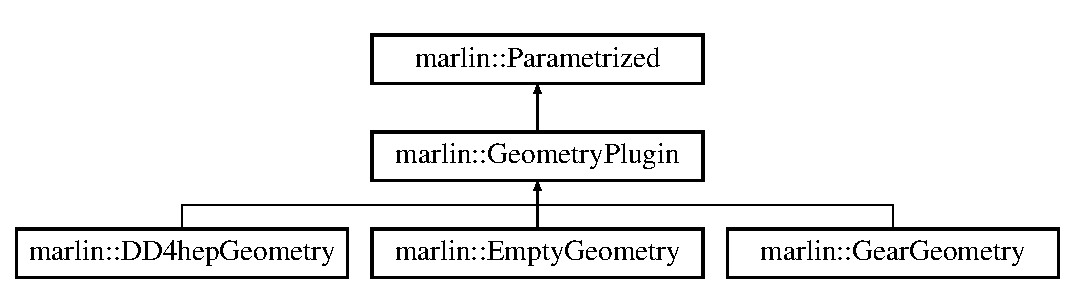
\includegraphics[height=3.000000cm]{classmarlin_1_1GeometryPlugin}
\end{center}
\end{figure}
\subsection*{Public Types}
\begin{DoxyCompactItemize}
\item 
\mbox{\label{classmarlin_1_1GeometryPlugin_a6297f7a0b1b21e21f5a45db3debc0b04}} 
using {\bfseries Logger} = Logging\+::\+Logger
\end{DoxyCompactItemize}
\subsection*{Public Member Functions}
\begin{DoxyCompactItemize}
\item 
\mbox{\label{classmarlin_1_1GeometryPlugin_af5b33c966fa36af014d2cc2229da5575}} 
{\bfseries Geometry\+Plugin} (const \textbf{ Geometry\+Plugin} \&)=delete
\item 
\mbox{\label{classmarlin_1_1GeometryPlugin_afdffe2c1f43716984d7fa7c6f0224008}} 
\textbf{ Geometry\+Plugin} \& {\bfseries operator=} (const \textbf{ Geometry\+Plugin} \&)=delete
\item 
\mbox{\label{classmarlin_1_1GeometryPlugin_aab2b227c1846264d395598fdc078aa39}} 
virtual std\+::type\+\_\+index \textbf{ type\+Index} () const =0
\begin{DoxyCompactList}\small\item\em Get a type index object from the geometry handle. \end{DoxyCompactList}\item 
\mbox{\label{classmarlin_1_1GeometryPlugin_a9ef3616301d48891e1dce6e516b43c03}} 
virtual void \textbf{ dump\+Geometry} () const =0
\begin{DoxyCompactList}\small\item\em Dump the geometry in the console. \end{DoxyCompactList}\item 
const std\+::string \& \textbf{ description} () const
\begin{DoxyCompactList}\small\item\em Get the geometry description. \end{DoxyCompactList}\item 
\mbox{\label{classmarlin_1_1GeometryPlugin_acb40da794bc079dbaeaac4cb986689ed}} 
const std\+::string \& \textbf{ type} () const
\begin{DoxyCompactList}\small\item\em Get the geometry type. \end{DoxyCompactList}\item 
void \textbf{ print} () const
\begin{DoxyCompactList}\small\item\em Print the complete geometry plugin description. \end{DoxyCompactList}\end{DoxyCompactItemize}
\subsection*{Protected Member Functions}
\begin{DoxyCompactItemize}
\item 
\textbf{ Geometry\+Plugin} (const std\+::string \&gtype)
\begin{DoxyCompactList}\small\item\em Constructor. \end{DoxyCompactList}\item 
\mbox{\label{classmarlin_1_1GeometryPlugin_a61c63cfed87e2da46176f01fa1ab2c57}} 
virtual void \textbf{ load\+Geometry} ()=0
\begin{DoxyCompactList}\small\item\em Load the geometry. \end{DoxyCompactList}\item 
\mbox{\label{classmarlin_1_1GeometryPlugin_a5ea49dd84089cf12a61741e974a9d31c}} 
virtual const void $\ast$ \textbf{ handle} () const =0
\begin{DoxyCompactList}\small\item\em Get a handle on the geometry instance. \end{DoxyCompactList}\item 
\mbox{\label{classmarlin_1_1GeometryPlugin_a6ed7abe0e05e566d99f3a4218fbe85dd}} 
virtual void \textbf{ destroy} ()=0
\begin{DoxyCompactList}\small\item\em Cleanup geometry. \end{DoxyCompactList}\item 
\mbox{\label{classmarlin_1_1GeometryPlugin_a4febb346aed5f4cd11757ab9a5eacae4}} 
const \textbf{ Application} \& \textbf{ app} () const
\begin{DoxyCompactList}\small\item\em Get the application in which the plugin has been created. \end{DoxyCompactList}\end{DoxyCompactItemize}
\subsection*{Protected Attributes}
\begin{DoxyCompactItemize}
\item 
\mbox{\label{classmarlin_1_1GeometryPlugin_a9fdd5653fcca61d6b302b6574b2e4da9}} 
const std\+::string \textbf{ \+\_\+type}
\begin{DoxyCompactList}\small\item\em The geometry type. \end{DoxyCompactList}\item 
\mbox{\label{classmarlin_1_1GeometryPlugin_a304aee7888e7af8d51b87fd8c952b375}} 
std\+::string \textbf{ \+\_\+description} \{\char`\"{}No \textbf{ description}\char`\"{}\}
\begin{DoxyCompactList}\small\item\em The geometry plugin description. \end{DoxyCompactList}\item 
\mbox{\label{classmarlin_1_1GeometryPlugin_ac89a395acf7e5287b95ab0bbae57811d}} 
Logger \textbf{ \+\_\+logger} \{nullptr\}
\begin{DoxyCompactList}\small\item\em The application logger. \end{DoxyCompactList}\item 
\mbox{\label{classmarlin_1_1GeometryPlugin_a637d9d0a550bb72c269a618d5a35812e}} 
bool \textbf{ \+\_\+dump\+Geometry} \{false\}
\begin{DoxyCompactList}\small\item\em Whether to dump the geometry on creation. \end{DoxyCompactList}\end{DoxyCompactItemize}
\subsection*{Friends}
\begin{DoxyCompactItemize}
\item 
\mbox{\label{classmarlin_1_1GeometryPlugin_a52d2717cba1ffaed0a4cde1918697357}} 
class {\bfseries Geometry\+Manager}
\end{DoxyCompactItemize}


\subsection{Detailed Description}
\doxyref{Geometry\+Plugin}{p.}{classmarlin_1_1GeometryPlugin} class Responsible for loading geometry in Marlin and providing access to it through the \doxyref{Geometry\+Manager}{p.}{classmarlin_1_1GeometryManager}. 

\subsection{Constructor \& Destructor Documentation}
\mbox{\label{classmarlin_1_1GeometryPlugin_a38e9cee84218dac5edcaaa785203d2b7}} 
\index{marlin\+::\+Geometry\+Plugin@{marlin\+::\+Geometry\+Plugin}!Geometry\+Plugin@{Geometry\+Plugin}}
\index{Geometry\+Plugin@{Geometry\+Plugin}!marlin\+::\+Geometry\+Plugin@{marlin\+::\+Geometry\+Plugin}}
\subsubsection{Geometry\+Plugin()}
{\footnotesize\ttfamily marlin\+::\+Geometry\+Plugin\+::\+Geometry\+Plugin (\begin{DoxyParamCaption}\item[{const std\+::string \&}]{gtype }\end{DoxyParamCaption})\hspace{0.3cm}{\ttfamily [protected]}}



Constructor. 

To be called by sub classes


\begin{DoxyParams}{Parameters}
{\em gtype} & the geometry type \\
\hline
\end{DoxyParams}


References \+\_\+dump\+Geometry, \+\_\+logger, marlin\+::\+Logging\+::create\+Logger(), and marlin\+::\+Parametrized\+::register\+Optional\+Parameter().



\subsection{Member Function Documentation}
\mbox{\label{classmarlin_1_1GeometryPlugin_ad9168e8b5a4b214befd8b87606fcfe94}} 
\index{marlin\+::\+Geometry\+Plugin@{marlin\+::\+Geometry\+Plugin}!description@{description}}
\index{description@{description}!marlin\+::\+Geometry\+Plugin@{marlin\+::\+Geometry\+Plugin}}
\subsubsection{description()}
{\footnotesize\ttfamily const std\+::string \& marlin\+::\+Geometry\+Plugin\+::description (\begin{DoxyParamCaption}{ }\end{DoxyParamCaption}) const\hspace{0.3cm}{\ttfamily [inline]}}



Get the geometry description. 

Can be set by sub-\/classes in constructor (protected) 

References \+\_\+description.



Referenced by print().

\mbox{\label{classmarlin_1_1GeometryPlugin_a3cf9992844455efae3a827c16002d9f4}} 
\index{marlin\+::\+Geometry\+Plugin@{marlin\+::\+Geometry\+Plugin}!print@{print}}
\index{print@{print}!marlin\+::\+Geometry\+Plugin@{marlin\+::\+Geometry\+Plugin}}
\subsubsection{print()}
{\footnotesize\ttfamily void marlin\+::\+Geometry\+Plugin\+::print (\begin{DoxyParamCaption}{ }\end{DoxyParamCaption}) const}



Print the complete geometry plugin description. 

The geometry is dumped if the verbosity level is less than D\+E\+B\+U\+G5 

References \+\_\+dump\+Geometry, \+\_\+logger, \+\_\+type, app(), marlin\+::\+Application\+::create\+Logger(), description(), dump\+Geometry(), handle(), load\+Geometry(), type(), and type\+Index().



The documentation for this class was generated from the following files\+:\begin{DoxyCompactItemize}
\item 
Geometry\+Plugin.\+h\item 
Geometry\+Plugin.\+cc\end{DoxyCompactItemize}

\section{marlin\+:\+:Hash\+Helper Class Reference}
\label{classmarlin_1_1HashHelper}\index{marlin\+::\+Hash\+Helper@{marlin\+::\+Hash\+Helper}}


\doxyref{Hash\+Helper}{p.}{classmarlin_1_1HashHelper} class Helper class to generate hash 64 id.  




{\ttfamily \#include $<$Utils.\+h$>$}

\subsection*{Static Public Member Functions}
\begin{DoxyCompactItemize}
\item 
\mbox{\label{classmarlin_1_1HashHelper_aac563f1c03d38c49906d5a1dc8cbccd0}} 
static constexpr unsigned long long int {\bfseries do\+Byte} (unsigned long long int hash, unsigned char val)
\item 
static unsigned long long int \textbf{ hash64} (const char $\ast$key)
\begin{DoxyCompactList}\small\item\em Generate a hash 64 from a string. \end{DoxyCompactList}\item 
\mbox{\label{classmarlin_1_1HashHelper_a5b7006e19019820fd26694c7ad2e63f7}} 
{\footnotesize template$<$typename T $>$ }\\static unsigned long long int \textbf{ type\+Hash64} ()
\begin{DoxyCompactList}\small\item\em Generate a hash 64 from the typeid name. \end{DoxyCompactList}\end{DoxyCompactItemize}


\subsection{Detailed Description}
\doxyref{Hash\+Helper}{p.}{classmarlin_1_1HashHelper} class Helper class to generate hash 64 id. 

\subsection{Member Function Documentation}
\mbox{\label{classmarlin_1_1HashHelper_a528975635645560b2749a9a2583bf505}} 
\index{marlin\+::\+Hash\+Helper@{marlin\+::\+Hash\+Helper}!hash64@{hash64}}
\index{hash64@{hash64}!marlin\+::\+Hash\+Helper@{marlin\+::\+Hash\+Helper}}
\subsubsection{hash64()}
{\footnotesize\ttfamily static unsigned long long int marlin\+::\+Hash\+Helper\+::hash64 (\begin{DoxyParamCaption}\item[{const char $\ast$}]{key }\end{DoxyParamCaption})\hspace{0.3cm}{\ttfamily [inline]}, {\ttfamily [static]}}



Generate a hash 64 from a string. 


\begin{DoxyParams}{Parameters}
{\em key} & the input string key \\
\hline
\end{DoxyParams}


The documentation for this class was generated from the following file\+:\begin{DoxyCompactItemize}
\item 
Utils.\+h\end{DoxyCompactItemize}

\section{marlin\+:\+:I\+Four\+Vector\+Smearer Class Reference}
\label{classmarlin_1_1IFourVectorSmearer}\index{marlin\+::\+I\+Four\+Vector\+Smearer@{marlin\+::\+I\+Four\+Vector\+Smearer}}


Interface for smearing of four vectors -\/ based on C\+L\+H\+E\+P\+::\+Hep\+Lorentz\+Vector.  




{\ttfamily \#include $<$I\+Four\+Vector\+Smearer.\+h$>$}

Inheritance diagram for marlin\+:\+:I\+Four\+Vector\+Smearer\+:\begin{figure}[H]
\begin{center}
\leavevmode
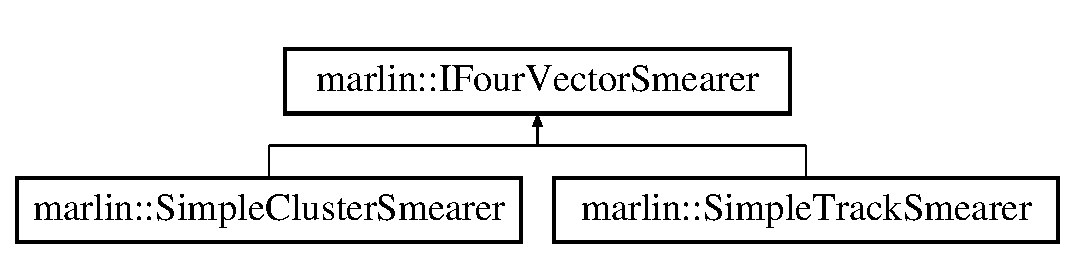
\includegraphics[height=2.000000cm]{classmarlin_1_1IFourVectorSmearer}
\end{center}
\end{figure}
\subsection*{Public Member Functions}
\begin{DoxyCompactItemize}
\item 
virtual \textbf{ $\sim$\+I\+Four\+Vector\+Smearer} ()
\begin{DoxyCompactList}\small\item\em Virtual d\textquotesingle{}tor. \end{DoxyCompactList}\item 
\mbox{\label{classmarlin_1_1IFourVectorSmearer_a69a3ece59f66350310e1eb1c696464ce}} 
virtual Hep\+Lorentz\+Vector \textbf{ smeared\+Four\+Vector} (const Hep\+Lorentz\+Vector \&v, int pdg\+Code)=0
\begin{DoxyCompactList}\small\item\em Smears the given four vector. \end{DoxyCompactList}\end{DoxyCompactItemize}


\subsection{Detailed Description}
Interface for smearing of four vectors -\/ based on C\+L\+H\+E\+P\+::\+Hep\+Lorentz\+Vector. 

\begin{DoxyAuthor}{Author}
F. Gaede, D\+E\+SY 
\end{DoxyAuthor}
\begin{DoxyVersion}{Version}

\end{DoxyVersion}
\begin{DoxyParagraph}{Id}
\doxyref{I\+Four\+Vector\+Smearer.\+h}{p.}{IFourVectorSmearer_8h_source},v 1.\+3 2006-\/03-\/30 16\+:12\+:16 gaede Exp 
\end{DoxyParagraph}


\subsection{Constructor \& Destructor Documentation}
\mbox{\label{classmarlin_1_1IFourVectorSmearer_aae702efdbe6007ea1db649ffc9bd7288}} 
\index{marlin\+::\+I\+Four\+Vector\+Smearer@{marlin\+::\+I\+Four\+Vector\+Smearer}!````~I\+Four\+Vector\+Smearer@{$\sim$\+I\+Four\+Vector\+Smearer}}
\index{````~I\+Four\+Vector\+Smearer@{$\sim$\+I\+Four\+Vector\+Smearer}!marlin\+::\+I\+Four\+Vector\+Smearer@{marlin\+::\+I\+Four\+Vector\+Smearer}}
\subsubsection{$\sim$\+I\+Four\+Vector\+Smearer()}
{\footnotesize\ttfamily virtual marlin\+::\+I\+Four\+Vector\+Smearer\+::$\sim$\+I\+Four\+Vector\+Smearer (\begin{DoxyParamCaption}{ }\end{DoxyParamCaption})\hspace{0.3cm}{\ttfamily [inline]}, {\ttfamily [virtual]}}



Virtual d\textquotesingle{}tor. 



The documentation for this class was generated from the following file\+:\begin{DoxyCompactItemize}
\item 
I\+Four\+Vector\+Smearer.\+h\end{DoxyCompactItemize}

\section{marlin\+:\+:I\+Parser Class Reference}
\label{classmarlin_1_1IParser}\index{marlin\+::\+I\+Parser@{marlin\+::\+I\+Parser}}


Interface for a parser of a steering file to be used with marlin.  




{\ttfamily \#include $<$I\+Parser.\+h$>$}

Inheritance diagram for marlin\+:\+:I\+Parser\+:\begin{figure}[H]
\begin{center}
\leavevmode
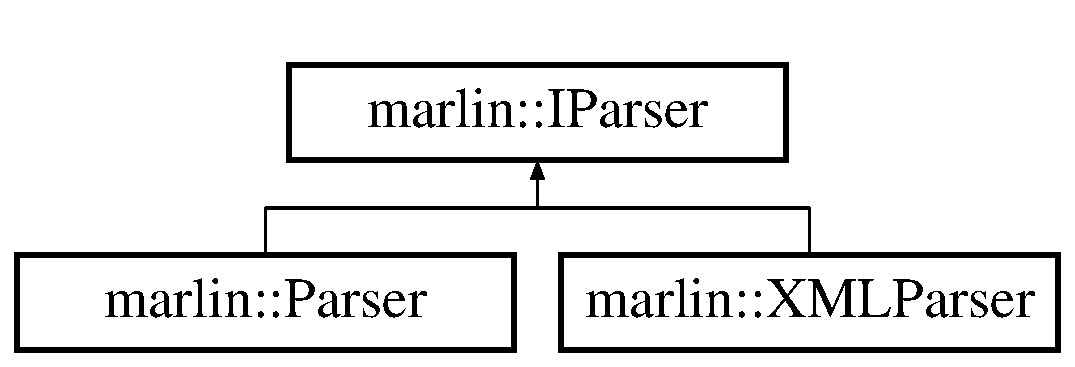
\includegraphics[height=2.000000cm]{classmarlin_1_1IParser}
\end{center}
\end{figure}
\subsection*{Public Member Functions}
\begin{DoxyCompactItemize}
\item 
\mbox{\label{classmarlin_1_1IParser_a7df3aa5d16d95ca2716915897a2a2cea}} 
virtual void \textbf{ parse} ()=0
\begin{DoxyCompactList}\small\item\em Parse the input file. \end{DoxyCompactList}\item 
\mbox{\label{classmarlin_1_1IParser_a45db55bec1004de22f41066bf490b74d}} 
virtual void \textbf{ set\+Cmd\+Line\+Parameters} (const Command\+Line\+Parameters\+Map \&cmdlineparams)=0
\begin{DoxyCompactList}\small\item\em set command line parameters \end{DoxyCompactList}\item 
\mbox{\label{classmarlin_1_1IParser_ab59774f48976295413b2e83931f2c477}} 
virtual std\+::shared\+\_\+ptr$<$ \textbf{ String\+Parameters} $>$ \textbf{ get\+Parameters} (const std\+::string \&section\+Name) const =0
\begin{DoxyCompactList}\small\item\em Return the \doxyref{String\+Parameters}{p.}{classmarlin_1_1StringParameters} defined for this section of the steering file. \end{DoxyCompactList}\item 
\mbox{\label{classmarlin_1_1IParser_aa65a00a0ce3aff902eb0e73578a5cd10}} 
virtual void \textbf{ write} (const std\+::string \&fname) const =0
\begin{DoxyCompactList}\small\item\em Write down the parsed file in a new file. \end{DoxyCompactList}\end{DoxyCompactItemize}


\subsection{Detailed Description}
Interface for a parser of a steering file to be used with marlin. 

\begin{DoxyAuthor}{Author}
F. Gaede, D\+E\+SY 
\end{DoxyAuthor}
\begin{DoxyVersion}{Version}

\end{DoxyVersion}
\begin{DoxyParagraph}{Id}
\doxyref{I\+Parser.\+h}{p.}{IParser_8h_source},v 1.\+2 2005-\/10-\/11 12\+:56\+:28 gaede Exp 
\end{DoxyParagraph}


The documentation for this class was generated from the following file\+:\begin{DoxyCompactItemize}
\item 
I\+Parser.\+h\end{DoxyCompactItemize}

\section{marlin\+:\+:I\+Reco\+Particle\+Factory Class Reference}
\label{classmarlin_1_1IRecoParticleFactory}\index{marlin\+::\+I\+Reco\+Particle\+Factory@{marlin\+::\+I\+Reco\+Particle\+Factory}}


Interface for a factory class that creates a Reconstructed\+Particle from an M\+C\+Particle.  




{\ttfamily \#include $<$I\+Reco\+Particle\+Factory.\+h$>$}

Inheritance diagram for marlin\+:\+:I\+Reco\+Particle\+Factory\+:\begin{figure}[H]
\begin{center}
\leavevmode
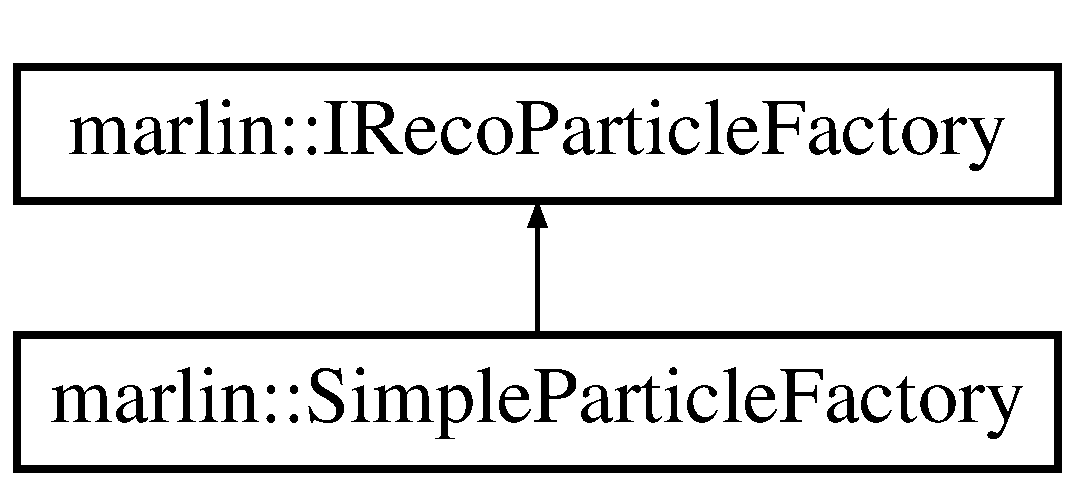
\includegraphics[height=2.000000cm]{classmarlin_1_1IRecoParticleFactory}
\end{center}
\end{figure}
\subsection*{Public Member Functions}
\begin{DoxyCompactItemize}
\item 
virtual \textbf{ $\sim$\+I\+Reco\+Particle\+Factory} ()
\begin{DoxyCompactList}\small\item\em Virtual d\textquotesingle{}tor. \end{DoxyCompactList}\item 
virtual lcio\+::\+Reconstructed\+Particle $\ast$ \textbf{ create\+Reconstructed\+Particle} (const lcio\+::\+M\+C\+Particle $\ast$mcp)=0
\begin{DoxyCompactList}\small\item\em The actual factory method that creates a new Reconstructed\+Particle for the given M\+C\+Particle. \end{DoxyCompactList}\end{DoxyCompactItemize}


\subsection{Detailed Description}
Interface for a factory class that creates a Reconstructed\+Particle from an M\+C\+Particle. 

\begin{DoxyAuthor}{Author}
F. Gaede, D\+E\+SY 
\end{DoxyAuthor}
\begin{DoxyVersion}{Version}

\end{DoxyVersion}
\begin{DoxyParagraph}{Id}
\doxyref{I\+Reco\+Particle\+Factory.\+h}{p.}{IRecoParticleFactory_8h_source},v 1.\+2 2005-\/10-\/11 12\+:56\+:28 gaede Exp 
\end{DoxyParagraph}


\subsection{Constructor \& Destructor Documentation}
\mbox{\label{classmarlin_1_1IRecoParticleFactory_ab3ef4fe43456f74a1f1f53a4f0dafe72}} 
\index{marlin\+::\+I\+Reco\+Particle\+Factory@{marlin\+::\+I\+Reco\+Particle\+Factory}!````~I\+Reco\+Particle\+Factory@{$\sim$\+I\+Reco\+Particle\+Factory}}
\index{````~I\+Reco\+Particle\+Factory@{$\sim$\+I\+Reco\+Particle\+Factory}!marlin\+::\+I\+Reco\+Particle\+Factory@{marlin\+::\+I\+Reco\+Particle\+Factory}}
\subsubsection{$\sim$\+I\+Reco\+Particle\+Factory()}
{\footnotesize\ttfamily virtual marlin\+::\+I\+Reco\+Particle\+Factory\+::$\sim$\+I\+Reco\+Particle\+Factory (\begin{DoxyParamCaption}{ }\end{DoxyParamCaption})\hspace{0.3cm}{\ttfamily [inline]}, {\ttfamily [virtual]}}



Virtual d\textquotesingle{}tor. 



References create\+Reconstructed\+Particle().



\subsection{Member Function Documentation}
\mbox{\label{classmarlin_1_1IRecoParticleFactory_a5f1c80596f818ee3b09db4567a171694}} 
\index{marlin\+::\+I\+Reco\+Particle\+Factory@{marlin\+::\+I\+Reco\+Particle\+Factory}!create\+Reconstructed\+Particle@{create\+Reconstructed\+Particle}}
\index{create\+Reconstructed\+Particle@{create\+Reconstructed\+Particle}!marlin\+::\+I\+Reco\+Particle\+Factory@{marlin\+::\+I\+Reco\+Particle\+Factory}}
\subsubsection{create\+Reconstructed\+Particle()}
{\footnotesize\ttfamily virtual lcio\+::\+Reconstructed\+Particle$\ast$ marlin\+::\+I\+Reco\+Particle\+Factory\+::create\+Reconstructed\+Particle (\begin{DoxyParamCaption}\item[{const lcio\+::\+M\+C\+Particle $\ast$}]{mcp }\end{DoxyParamCaption})\hspace{0.3cm}{\ttfamily [pure virtual]}}



The actual factory method that creates a new Reconstructed\+Particle for the given M\+C\+Particle. 

N\+U\+LL if no Reconstructed\+Particle should be created due to detector acceptance. 

Implemented in \textbf{ marlin\+::\+Simple\+Particle\+Factory} \doxyref{}{p.}{classmarlin_1_1SimpleParticleFactory_a2c050bb3a0c06aadcb5ef9c552b409f7}.



Referenced by marlin\+::\+Simple\+Fast\+M\+C\+Processor\+::process\+Event(), and $\sim$\+I\+Reco\+Particle\+Factory().



The documentation for this class was generated from the following file\+:\begin{DoxyCompactItemize}
\item 
I\+Reco\+Particle\+Factory.\+h\end{DoxyCompactItemize}

\section{marlin\+:\+:I\+Scheduler Class Reference}
\label{classmarlin_1_1IScheduler}\index{marlin\+::\+I\+Scheduler@{marlin\+::\+I\+Scheduler}}


\doxyref{I\+Scheduler}{p.}{classmarlin_1_1IScheduler} interface Interface for implementing a scheduling algorithm for event processing.  




{\ttfamily \#include $<$I\+Scheduler.\+h$>$}

Inheritance diagram for marlin\+:\+:I\+Scheduler\+:\begin{figure}[H]
\begin{center}
\leavevmode
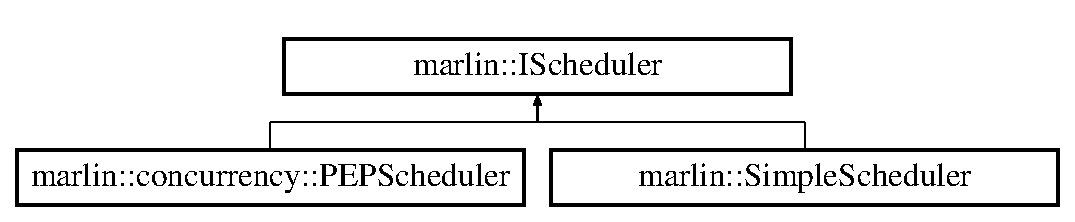
\includegraphics[height=2.000000cm]{classmarlin_1_1IScheduler}
\end{center}
\end{figure}
\subsection*{Public Member Functions}
\begin{DoxyCompactItemize}
\item 
virtual void \textbf{ init} (\textbf{ Application} $\ast$app)=0
\begin{DoxyCompactList}\small\item\em Initialize the scheduler with app parameters. \end{DoxyCompactList}\item 
\mbox{\label{classmarlin_1_1IScheduler_a5b1ff631c643779e4504985ea031cb3e}} 
virtual void \textbf{ end} ()=0
\begin{DoxyCompactList}\small\item\em Terminate the scheduler activites Cleanup memory, etc ... \end{DoxyCompactList}\item 
virtual void \textbf{ process\+Run\+Header} (std\+::shared\+\_\+ptr$<$ E\+V\+E\+N\+T\+::\+L\+C\+Run\+Header $>$ rhdr)=0
\begin{DoxyCompactList}\small\item\em Process a run header. \end{DoxyCompactList}\item 
virtual void \textbf{ push\+Event} (std\+::shared\+\_\+ptr$<$ E\+V\+E\+N\+T\+::\+L\+C\+Event $>$ event)=0
\begin{DoxyCompactList}\small\item\em Push a new event to the scheduler for processing. \end{DoxyCompactList}\item 
virtual void \textbf{ pop\+Finished\+Events} (std\+::vector$<$ std\+::shared\+\_\+ptr$<$ E\+V\+E\+N\+T\+::\+L\+C\+Event $>$$>$ \&events)=0
\begin{DoxyCompactList}\small\item\em Retrieve finished events from the scheduler. \end{DoxyCompactList}\item 
\mbox{\label{classmarlin_1_1IScheduler_a040cba5dd23490c8727a8d2f2c878bb0}} 
virtual std\+::size\+\_\+t \textbf{ free\+Slots} () const =0
\begin{DoxyCompactList}\small\item\em Get the number of free event slots. \end{DoxyCompactList}\end{DoxyCompactItemize}


\subsection{Detailed Description}
\doxyref{I\+Scheduler}{p.}{classmarlin_1_1IScheduler} interface Interface for implementing a scheduling algorithm for event processing. 

The scheduling can be sequential or parallel (inter-\/event / intra-\/event / both). See implementation classes for more details. 

\subsection{Member Function Documentation}
\mbox{\label{classmarlin_1_1IScheduler_a043b3fac1587242d8937aaca575d0a8a}} 
\index{marlin\+::\+I\+Scheduler@{marlin\+::\+I\+Scheduler}!init@{init}}
\index{init@{init}!marlin\+::\+I\+Scheduler@{marlin\+::\+I\+Scheduler}}
\subsubsection{init()}
{\footnotesize\ttfamily virtual void marlin\+::\+I\+Scheduler\+::init (\begin{DoxyParamCaption}\item[{\textbf{ Application} $\ast$}]{app }\end{DoxyParamCaption})\hspace{0.3cm}{\ttfamily [pure virtual]}}



Initialize the scheduler with app parameters. 


\begin{DoxyParams}{Parameters}
{\em app} & the application in which the scheduler runs \\
\hline
\end{DoxyParams}


Implemented in \textbf{ marlin\+::concurrency\+::\+P\+E\+P\+Scheduler} \doxyref{}{p.}{classmarlin_1_1concurrency_1_1PEPScheduler_a0073eec7813c50ab53aa5af128a6c774}, and \textbf{ marlin\+::\+Simple\+Scheduler} \doxyref{}{p.}{classmarlin_1_1SimpleScheduler_aaa28a26180c4daa4fd8f86145fc2677d}.

\mbox{\label{classmarlin_1_1IScheduler_a30b54277206eca898a0ea8ac6f44d883}} 
\index{marlin\+::\+I\+Scheduler@{marlin\+::\+I\+Scheduler}!pop\+Finished\+Events@{pop\+Finished\+Events}}
\index{pop\+Finished\+Events@{pop\+Finished\+Events}!marlin\+::\+I\+Scheduler@{marlin\+::\+I\+Scheduler}}
\subsubsection{pop\+Finished\+Events()}
{\footnotesize\ttfamily virtual void marlin\+::\+I\+Scheduler\+::pop\+Finished\+Events (\begin{DoxyParamCaption}\item[{std\+::vector$<$ std\+::shared\+\_\+ptr$<$ E\+V\+E\+N\+T\+::\+L\+C\+Event $>$$>$ \&}]{events }\end{DoxyParamCaption})\hspace{0.3cm}{\ttfamily [pure virtual]}}



Retrieve finished events from the scheduler. 


\begin{DoxyParams}{Parameters}
{\em events} & the list of event to retrieve \\
\hline
\end{DoxyParams}


Implemented in \textbf{ marlin\+::concurrency\+::\+P\+E\+P\+Scheduler} \doxyref{}{p.}{classmarlin_1_1concurrency_1_1PEPScheduler_a1ea04a94fdbe98fc3c9c0802a3bff3c5}, and \textbf{ marlin\+::\+Simple\+Scheduler} \doxyref{}{p.}{classmarlin_1_1SimpleScheduler_a3e7638dbc2a22e94053e1d7dc9fe581f}.

\mbox{\label{classmarlin_1_1IScheduler_a2f77a7a3b74b875bc492311f8971ff37}} 
\index{marlin\+::\+I\+Scheduler@{marlin\+::\+I\+Scheduler}!process\+Run\+Header@{process\+Run\+Header}}
\index{process\+Run\+Header@{process\+Run\+Header}!marlin\+::\+I\+Scheduler@{marlin\+::\+I\+Scheduler}}
\subsubsection{process\+Run\+Header()}
{\footnotesize\ttfamily virtual void marlin\+::\+I\+Scheduler\+::process\+Run\+Header (\begin{DoxyParamCaption}\item[{std\+::shared\+\_\+ptr$<$ E\+V\+E\+N\+T\+::\+L\+C\+Run\+Header $>$}]{rhdr }\end{DoxyParamCaption})\hspace{0.3cm}{\ttfamily [pure virtual]}}



Process a run header. 


\begin{DoxyParams}{Parameters}
{\em rhdr} & the run header to process \\
\hline
\end{DoxyParams}


Implemented in \textbf{ marlin\+::concurrency\+::\+P\+E\+P\+Scheduler} \doxyref{}{p.}{classmarlin_1_1concurrency_1_1PEPScheduler_a83744239f6f487f3d515ec126d10096e}, and \textbf{ marlin\+::\+Simple\+Scheduler} \doxyref{}{p.}{classmarlin_1_1SimpleScheduler_a3f233d79be2cffcb94e14b871eb7e2fc}.

\mbox{\label{classmarlin_1_1IScheduler_a336598b4b1a9643fabcc1487944208d2}} 
\index{marlin\+::\+I\+Scheduler@{marlin\+::\+I\+Scheduler}!push\+Event@{push\+Event}}
\index{push\+Event@{push\+Event}!marlin\+::\+I\+Scheduler@{marlin\+::\+I\+Scheduler}}
\subsubsection{push\+Event()}
{\footnotesize\ttfamily virtual void marlin\+::\+I\+Scheduler\+::push\+Event (\begin{DoxyParamCaption}\item[{std\+::shared\+\_\+ptr$<$ E\+V\+E\+N\+T\+::\+L\+C\+Event $>$}]{event }\end{DoxyParamCaption})\hspace{0.3cm}{\ttfamily [pure virtual]}}



Push a new event to the scheduler for processing. 


\begin{DoxyParams}{Parameters}
{\em event} & the event to push \\
\hline
\end{DoxyParams}


Implemented in \textbf{ marlin\+::concurrency\+::\+P\+E\+P\+Scheduler} \doxyref{}{p.}{classmarlin_1_1concurrency_1_1PEPScheduler_a2958256e8d5b36cb00cf0326f2c01084}, and \textbf{ marlin\+::\+Simple\+Scheduler} \doxyref{}{p.}{classmarlin_1_1SimpleScheduler_a9e18cd853bf832b284b5e343d0b2399e}.



The documentation for this class was generated from the following file\+:\begin{DoxyCompactItemize}
\item 
I\+Scheduler.\+h\end{DoxyCompactItemize}

\section{marlin\+:\+:Is\+First\+Event Struct Reference}
\label{structmarlin_1_1IsFirstEvent}\index{marlin\+::\+Is\+First\+Event@{marlin\+::\+Is\+First\+Event}}
Inheritance diagram for marlin\+:\+:Is\+First\+Event\+:\begin{figure}[H]
\begin{center}
\leavevmode
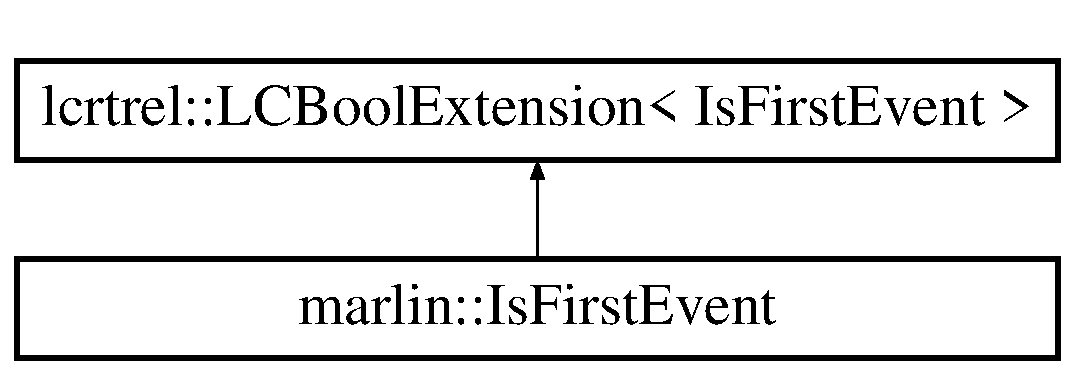
\includegraphics[height=2.000000cm]{structmarlin_1_1IsFirstEvent}
\end{center}
\end{figure}


The documentation for this struct was generated from the following file\+:\begin{DoxyCompactItemize}
\item 
Event\+Extensions.\+h\end{DoxyCompactItemize}

\section{marlin\+:\+:L\+C\+I\+O\+File\+Source Class Reference}
\label{classmarlin_1_1LCIOFileSource}\index{marlin\+::\+L\+C\+I\+O\+File\+Source@{marlin\+::\+L\+C\+I\+O\+File\+Source}}


\doxyref{L\+C\+I\+O\+File\+Source}{p.}{classmarlin_1_1LCIOFileSource} class.  


Inheritance diagram for marlin\+:\+:L\+C\+I\+O\+File\+Source\+:\begin{figure}[H]
\begin{center}
\leavevmode
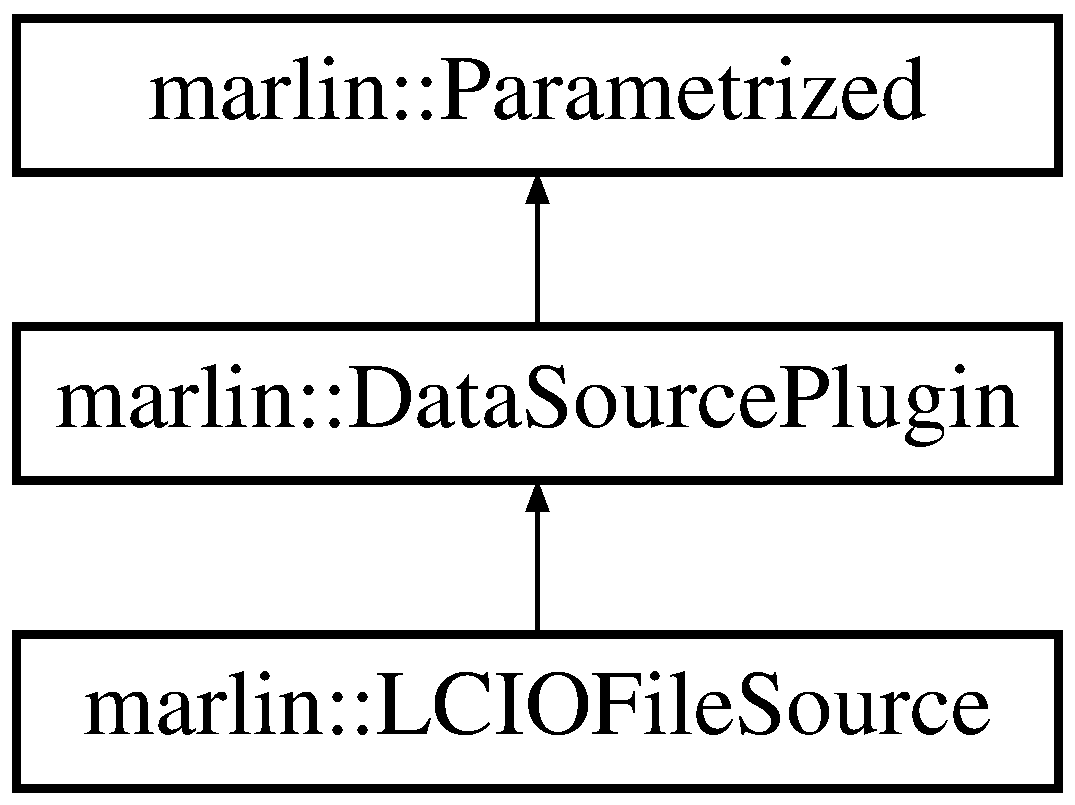
\includegraphics[height=3.000000cm]{classmarlin_1_1LCIOFileSource}
\end{center}
\end{figure}
\subsection*{Public Member Functions}
\begin{DoxyCompactItemize}
\item 
\mbox{\label{classmarlin_1_1LCIOFileSource_a260cb9019ababeeeda6c7adab29e5eb8}} 
void \textbf{ init} ()
\begin{DoxyCompactList}\small\item\em Initialize the plugin. \end{DoxyCompactList}\item 
bool \textbf{ read\+One} ()
\begin{DoxyCompactList}\small\item\em Read one record from the input stream. \end{DoxyCompactList}\end{DoxyCompactItemize}
\subsection*{Additional Inherited Members}


\subsection{Detailed Description}
\doxyref{L\+C\+I\+O\+File\+Source}{p.}{classmarlin_1_1LCIOFileSource} class. 

\subsection{Member Function Documentation}
\mbox{\label{classmarlin_1_1LCIOFileSource_aed4e06595dbb4b22b50766369d0c4809}} 
\index{marlin\+::\+L\+C\+I\+O\+File\+Source@{marlin\+::\+L\+C\+I\+O\+File\+Source}!read\+One@{read\+One}}
\index{read\+One@{read\+One}!marlin\+::\+L\+C\+I\+O\+File\+Source@{marlin\+::\+L\+C\+I\+O\+File\+Source}}
\subsubsection{read\+One()}
{\footnotesize\ttfamily bool marlin\+::\+L\+C\+I\+O\+File\+Source\+::read\+One (\begin{DoxyParamCaption}{ }\end{DoxyParamCaption})\hspace{0.3cm}{\ttfamily [virtual]}}



Read one record from the input stream. 

Users must call \doxyref{process\+Run\+Header()}{p.}{classmarlin_1_1DataSourcePlugin_a769e257658ee89c176857191773c26b3} or \doxyref{process\+Event()}{p.}{classmarlin_1_1DataSourcePlugin_add4afa8b047d3a2e4e33a9957e75d9bb} to forward it to the framework. Returns true on success. If the end of the stream is reached, return false. 

Implements \textbf{ marlin\+::\+Data\+Source\+Plugin} \doxyref{}{p.}{classmarlin_1_1DataSourcePlugin_a9e174b63facdc108425e79fca9022404}.



The documentation for this class was generated from the following file\+:\begin{DoxyCompactItemize}
\item 
L\+C\+I\+O\+File\+Source.\+cc\end{DoxyCompactItemize}

\section{marlin\+:\+:L\+C\+I\+O\+Output\+Processor Class Reference}
\label{classmarlin_1_1LCIOOutputProcessor}\index{marlin\+::\+L\+C\+I\+O\+Output\+Processor@{marlin\+::\+L\+C\+I\+O\+Output\+Processor}}


Default output processor.  


Inheritance diagram for marlin\+:\+:L\+C\+I\+O\+Output\+Processor\+:\begin{figure}[H]
\begin{center}
\leavevmode
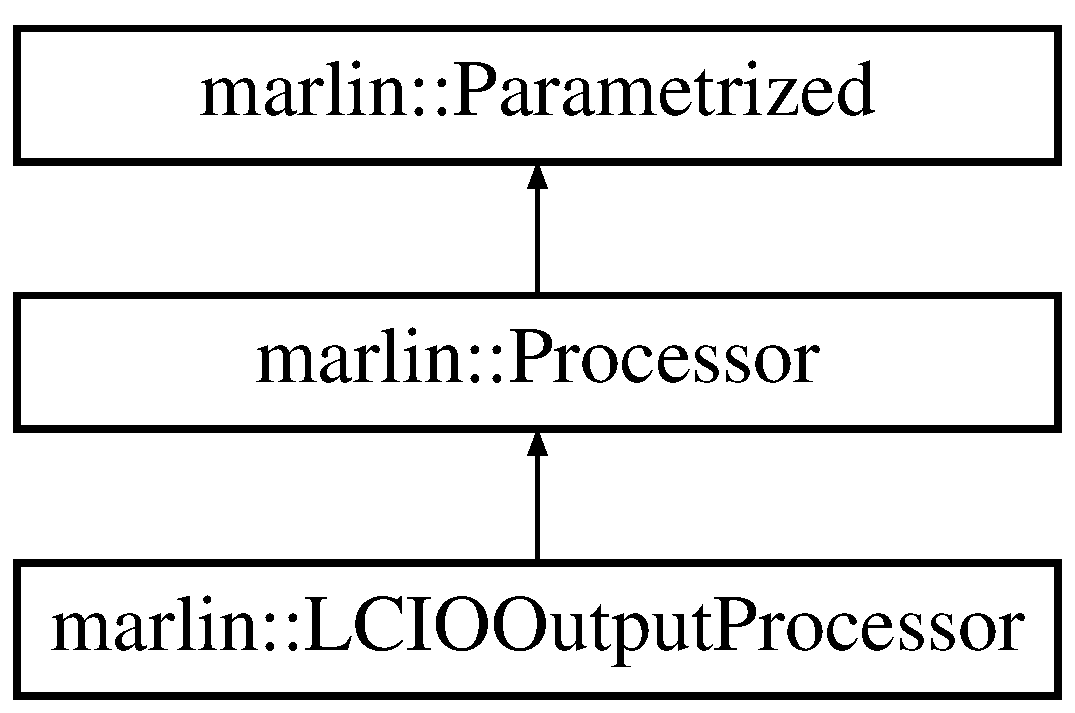
\includegraphics[height=3.000000cm]{classmarlin_1_1LCIOOutputProcessor}
\end{center}
\end{figure}
\subsection*{Public Member Functions}
\begin{DoxyCompactItemize}
\item 
\mbox{\label{classmarlin_1_1LCIOOutputProcessor_a425a069f55fd2f5a304cfb7f281c720c}} 
{\bfseries L\+C\+I\+O\+Output\+Processor} (const \textbf{ L\+C\+I\+O\+Output\+Processor} \&)=delete
\item 
\mbox{\label{classmarlin_1_1LCIOOutputProcessor_a64e6d2939a1e42ed9d1f26365e59b920}} 
\textbf{ L\+C\+I\+O\+Output\+Processor} \& {\bfseries operator=} (const \textbf{ L\+C\+I\+O\+Output\+Processor} \&)=delete
\item 
\mbox{\label{classmarlin_1_1LCIOOutputProcessor_ac53eb5a49c585a26f7177c3841185c97}} 
\textbf{ Processor} $\ast$ \textbf{ new\+Processor} ()
\begin{DoxyCompactList}\small\item\em Return a new instance of the processor (factory method) \end{DoxyCompactList}\item 
\mbox{\label{classmarlin_1_1LCIOOutputProcessor_a23c540ec3d9be10fc4e4b5431bfe64e4}} 
void \textbf{ init} ()
\begin{DoxyCompactList}\small\item\em Open the L\+C\+IO outputfile. \end{DoxyCompactList}\item 
\mbox{\label{classmarlin_1_1LCIOOutputProcessor_af7db9cfb92e19cff720c5171af86a4c8}} 
void \textbf{ process\+Run\+Header} (E\+V\+E\+N\+T\+::\+L\+C\+Run\+Header $\ast$run)
\begin{DoxyCompactList}\small\item\em Write every run header. \end{DoxyCompactList}\item 
\mbox{\label{classmarlin_1_1LCIOOutputProcessor_a07ab3e9f18f80ad76372cdfa17b674e2}} 
void \textbf{ process\+Event} (E\+V\+E\+N\+T\+::\+L\+C\+Event $\ast$evt)
\begin{DoxyCompactList}\small\item\em Write every event. \end{DoxyCompactList}\item 
\mbox{\label{classmarlin_1_1LCIOOutputProcessor_a03a7ac4d65110b0555dbfdec51a819a1}} 
void \textbf{ end} ()
\begin{DoxyCompactList}\small\item\em Close outputfile. \end{DoxyCompactList}\item 
\mbox{\label{classmarlin_1_1LCIOOutputProcessor_a861bcbba9e0af1094af55672a3ce0067}} 
void \textbf{ drop\+Collections} (E\+V\+E\+N\+T\+::\+L\+C\+Event $\ast$evt)
\begin{DoxyCompactList}\small\item\em Drops the collections specified in the steering file parameters Drop\+Collection\+Names and Drop\+Collection\+Types. \end{DoxyCompactList}\end{DoxyCompactItemize}
\subsection*{Additional Inherited Members}


\subsection{Detailed Description}
Default output processor. 

If active every event is writen to the specified L\+C\+IO file. Make sure that the processor is the last one in your list of active processors. You can optionally drop some collections from the event before it gets written to the file, e.\+g. you can drop all collections of types Sim\+Calorimeter\+Hit and Sim\+Tracker\+Hit. It is the users responsibility to check whether the droped objects are still referenced by other objects (e.\+g. L\+C\+Relations) and drop those collections as well -\/ if needed. If Calorimeter\+Hit and Tracker\+Hit objects are droped then Tracks and clusters will be store w/o pointers to hits.

\subparagraph*{Output}

file containing the L\+C\+IO events


\begin{DoxyParams}{Parameters}
{\em L\+C\+I\+O\+Output\+File} & name of outputfile incl. path \\
\hline
{\em L\+C\+I\+O\+Write\+Mode} & W\+R\+I\+T\+E\+\_\+\+N\+EW, W\+R\+I\+T\+E\+\_\+\+A\+P\+P\+E\+ND [optional] \\
\hline
{\em Drop\+Collection\+Names} & name of collections to be droped [optional] \\
\hline
{\em Drop\+Collection\+Types} & type of collections to be droped [optional]\\
\hline
{\em Drop\+Collection\+Names} & drops the named collections from the event \\
\hline
{\em Drop\+Collection\+Types} & drops all collections of the given type from the event \\
\hline
{\em L\+C\+I\+O\+Output\+File} & name of output file \\
\hline
{\em L\+C\+I\+O\+Write\+Mode} & write mode for output file\+: W\+R\+I\+T\+E\+\_\+\+A\+P\+P\+E\+ND or W\+R\+I\+T\+E\+\_\+\+N\+EW \\
\hline
{\em Keep\+Collection\+Names} & names of collections that are to be kept unconditionally \\
\hline
{\em full\+Subset\+Collections} & optionally write all objects in subset collections to the file\\
\hline
\end{DoxyParams}
\begin{DoxyAuthor}{Author}
F. Gaede, D\+E\+SY 
\end{DoxyAuthor}
\begin{DoxyVersion}{Version}

\end{DoxyVersion}
\begin{DoxyParagraph}{Id}
L\+C\+I\+O\+Output\+Processor.\+h,v 1.\+8 2008-\/04-\/15 10\+:14\+:24 gaede Exp 
\end{DoxyParagraph}


The documentation for this class was generated from the following file\+:\begin{DoxyCompactItemize}
\item 
L\+C\+I\+O\+Output\+Processor.\+cc\end{DoxyCompactItemize}

\section{marlin\+:\+:X\+M\+L\+Parser\+:\+:L\+C\+Tokenizer Class Reference}
\label{classmarlin_1_1XMLParser_1_1LCTokenizer}\index{marlin\+::\+X\+M\+L\+Parser\+::\+L\+C\+Tokenizer@{marlin\+::\+X\+M\+L\+Parser\+::\+L\+C\+Tokenizer}}


Helper class for \doxyref{X\+M\+L\+Parser}{p.}{classmarlin_1_1XMLParser}.  




{\ttfamily \#include $<$X\+M\+L\+Parser.\+h$>$}

\subsection*{Public Member Functions}
\begin{DoxyCompactItemize}
\item 
\mbox{\label{classmarlin_1_1XMLParser_1_1LCTokenizer_a6be937a517f1d429e4174a5f2c45422f}} 
{\bfseries L\+C\+Tokenizer} (std\+::vector$<$ std\+::string $>$ \&tokens, char del)
\item 
\mbox{\label{classmarlin_1_1XMLParser_1_1LCTokenizer_af75f64fa413370ea2286565dbafac1fa}} 
void {\bfseries operator()} (const char \&c)
\item 
\mbox{\label{classmarlin_1_1XMLParser_1_1LCTokenizer_a9d91350675fc8a13b9b27e86cd9d1a62}} 
std\+::vector$<$ std\+::string $>$ \& {\bfseries result} ()
\end{DoxyCompactItemize}


\subsection{Detailed Description}
Helper class for \doxyref{X\+M\+L\+Parser}{p.}{classmarlin_1_1XMLParser}. 

The documentation for this class was generated from the following file\+:\begin{DoxyCompactItemize}
\item 
X\+M\+L\+Parser.\+h\end{DoxyCompactItemize}

\section{marlin\+:\+:L\+C\+Tokenizer Class Reference}
\label{classmarlin_1_1LCTokenizer}\index{marlin\+::\+L\+C\+Tokenizer@{marlin\+::\+L\+C\+Tokenizer}}


Helper class for \doxyref{Parser}{p.}{classmarlin_1_1Parser}.  




{\ttfamily \#include $<$Parser.\+h$>$}

\subsection*{Public Member Functions}
\begin{DoxyCompactItemize}
\item 
\mbox{\label{classmarlin_1_1LCTokenizer_ad352c339aa4862d057e30e3483973325}} 
{\bfseries L\+C\+Tokenizer} (std\+::vector$<$ std\+::string $>$ \&tokens, char del)
\item 
\mbox{\label{classmarlin_1_1LCTokenizer_a6e1c1c694b8c464730ec769ee6e72a4a}} 
void {\bfseries operator()} (const char \&c)
\item 
\mbox{\label{classmarlin_1_1LCTokenizer_ad1ea074769fda7e11ea4c42f2d466146}} 
std\+::vector$<$ std\+::string $>$ \& {\bfseries result} ()
\end{DoxyCompactItemize}


\subsection{Detailed Description}
Helper class for \doxyref{Parser}{p.}{classmarlin_1_1Parser}. 

The documentation for this class was generated from the following file\+:\begin{DoxyCompactItemize}
\item 
Parser.\+h\end{DoxyCompactItemize}

\section{marlin\+:\+:Logger\+Manager Class Reference}
\label{classmarlin_1_1LoggerManager}\index{marlin\+::\+Logger\+Manager@{marlin\+::\+Logger\+Manager}}


\doxyref{Logger\+Manager}{p.}{classmarlin_1_1LoggerManager} class Responsible for configuring logger for a given application.  




{\ttfamily \#include $<$Logger\+Manager.\+h$>$}

\subsection*{Public Types}
\begin{DoxyCompactItemize}
\item 
\mbox{\label{classmarlin_1_1LoggerManager_a315868dad72cfd81b24dd2a0f911ff79}} 
using {\bfseries Logger} = Logging\+::\+Logger
\end{DoxyCompactItemize}
\subsection*{Public Member Functions}
\begin{DoxyCompactItemize}
\item 
\mbox{\label{classmarlin_1_1LoggerManager_a854e4c9f8a1e266d29477a706634fc24}} 
{\bfseries Logger\+Manager} (const \textbf{ Logger\+Manager} \&)=delete
\item 
\mbox{\label{classmarlin_1_1LoggerManager_a11c16b7548556d672f186d4b290d2526}} 
\textbf{ Logger\+Manager} \& {\bfseries operator=} (const \textbf{ Logger\+Manager} \&)=delete
\item 
\mbox{\label{classmarlin_1_1LoggerManager_ac33a972dffe1dcf4e02c6276f01b9106}} 
\textbf{ Logger\+Manager} ()
\begin{DoxyCompactList}\small\item\em Constructor. \end{DoxyCompactList}\item 
void \textbf{ init} (const \textbf{ Application} $\ast$app)
\begin{DoxyCompactList}\small\item\em Initialize the manager and the manager using the application settings. \end{DoxyCompactList}\item 
\mbox{\label{classmarlin_1_1LoggerManager_ad2ef4715cec9a1e8ad354f3149b721c2}} 
Logger \textbf{ main\+Logger} () const
\begin{DoxyCompactList}\small\item\em Get the main logger instance (not the global one) \end{DoxyCompactList}\item 
Logger \textbf{ create\+Logger} (const std\+::string \&name) const
\begin{DoxyCompactList}\small\item\em Create a new logger instance. \end{DoxyCompactList}\item 
void \textbf{ set\+Level} (const std\+::string \&level)
\begin{DoxyCompactList}\small\item\em Set the verbosity level of both the main and global loggers. \end{DoxyCompactList}\item 
\mbox{\label{classmarlin_1_1LoggerManager_ab1b6490a226f74d7acaf957b7282fe1c}} 
bool \textbf{ is\+Initialized} () const
\begin{DoxyCompactList}\small\item\em Whether the logger manager has been initialized. \end{DoxyCompactList}\end{DoxyCompactItemize}


\subsection{Detailed Description}
\doxyref{Logger\+Manager}{p.}{classmarlin_1_1LoggerManager} class Responsible for configuring logger for a given application. 

Can possibly configure the global logger instance. 

\subsection{Member Function Documentation}
\mbox{\label{classmarlin_1_1LoggerManager_a2343a9ded6d465718b113c9a530ea64d}} 
\index{marlin\+::\+Logger\+Manager@{marlin\+::\+Logger\+Manager}!create\+Logger@{create\+Logger}}
\index{create\+Logger@{create\+Logger}!marlin\+::\+Logger\+Manager@{marlin\+::\+Logger\+Manager}}
\subsubsection{create\+Logger()}
{\footnotesize\ttfamily Logger\+Manager\+::\+Logger marlin\+::\+Logger\+Manager\+::create\+Logger (\begin{DoxyParamCaption}\item[{const std\+::string \&}]{name }\end{DoxyParamCaption}) const}



Create a new logger instance. 

The logger shares the same sinks as the main logger


\begin{DoxyParams}{Parameters}
{\em name} & the logger name \\
\hline
\end{DoxyParams}


References marlin\+::\+Logging\+::create\+Logger(), is\+Initialized(), and main\+Logger().

\mbox{\label{classmarlin_1_1LoggerManager_a8b3970dc892184d30833ad16017c245d}} 
\index{marlin\+::\+Logger\+Manager@{marlin\+::\+Logger\+Manager}!init@{init}}
\index{init@{init}!marlin\+::\+Logger\+Manager@{marlin\+::\+Logger\+Manager}}
\subsubsection{init()}
{\footnotesize\ttfamily void marlin\+::\+Logger\+Manager\+::init (\begin{DoxyParamCaption}\item[{const \textbf{ Application} $\ast$}]{app }\end{DoxyParamCaption})}



Initialize the manager and the manager using the application settings. 


\begin{DoxyParams}{Parameters}
{\em app} & the application \\
\hline
\end{DoxyParams}


References marlin\+::\+Application\+::global\+Parameters(), main\+Logger(), marlin\+::\+Application\+::program(), and set\+Level().

\mbox{\label{classmarlin_1_1LoggerManager_a3ecf7748893c290773da233a6535f8eb}} 
\index{marlin\+::\+Logger\+Manager@{marlin\+::\+Logger\+Manager}!set\+Level@{set\+Level}}
\index{set\+Level@{set\+Level}!marlin\+::\+Logger\+Manager@{marlin\+::\+Logger\+Manager}}
\subsubsection{set\+Level()}
{\footnotesize\ttfamily void marlin\+::\+Logger\+Manager\+::set\+Level (\begin{DoxyParamCaption}\item[{const std\+::string \&}]{level }\end{DoxyParamCaption})}



Set the verbosity level of both the main and global loggers. 


\begin{DoxyParams}{Parameters}
{\em level} & the verbosity level to set \\
\hline
\end{DoxyParams}


References main\+Logger().



Referenced by init().



The documentation for this class was generated from the following files\+:\begin{DoxyCompactItemize}
\item 
Logger\+Manager.\+h\item 
Logger\+Manager.\+cc\end{DoxyCompactItemize}

\section{marlin\+:\+:Logging Class Reference}
\label{classmarlin_1_1Logging}\index{marlin\+::\+Logging@{marlin\+::\+Logging}}


\doxyref{Logging}{p.}{classmarlin_1_1Logging} class.  




{\ttfamily \#include $<$Logging.\+h$>$}

\subsection*{Public Types}
\begin{DoxyCompactItemize}
\item 
\mbox{\label{classmarlin_1_1Logging_ad18616e327b3bad4f01cd8c314aaba9b}} 
using {\bfseries mutex\+\_\+type} = streamlog\+::st
\item 
\mbox{\label{classmarlin_1_1Logging_ac3f289d27b887eaa79a72bab0a0a53da}} 
using {\bfseries Logger} = std\+::shared\+\_\+ptr$<$ streamlog\+::logstreamT$<$ mutex\+\_\+type $>$ $>$
\item 
\mbox{\label{classmarlin_1_1Logging_af5e3b01d3070f1b48bee0c1e5c0ba092}} 
using {\bfseries Stream\+Type} = Logger\+::element\+\_\+type\+::stream\+\_\+type
\end{DoxyCompactItemize}
\subsection*{Static Public Member Functions}
\begin{DoxyCompactItemize}
\item 
static Logger \textbf{ create\+Logger} (const std\+::string \&name)
\begin{DoxyCompactList}\small\item\em Create a standalone logger instance. \end{DoxyCompactList}\end{DoxyCompactItemize}


\subsection{Detailed Description}
\doxyref{Logging}{p.}{classmarlin_1_1Logging} class. 

Defines the basic logging functionalities in Marlin. For a more application oriented configuration, see \doxyref{Logger\+Manager.\+h}{p.}{LoggerManager_8h_source} 

\subsection{Member Function Documentation}
\mbox{\label{classmarlin_1_1Logging_a71216e83ad67a98ff2dad9a547a6c3b6}} 
\index{marlin\+::\+Logging@{marlin\+::\+Logging}!create\+Logger@{create\+Logger}}
\index{create\+Logger@{create\+Logger}!marlin\+::\+Logging@{marlin\+::\+Logging}}
\subsubsection{create\+Logger()}
{\footnotesize\ttfamily Logging\+::\+Logger marlin\+::\+Logging\+::create\+Logger (\begin{DoxyParamCaption}\item[{const std\+::string \&}]{name }\end{DoxyParamCaption})\hspace{0.3cm}{\ttfamily [static]}}



Create a standalone logger instance. 


\begin{DoxyParams}{Parameters}
{\em name} & the logger name \\
\hline
\end{DoxyParams}


Referenced by marlin\+::\+Logger\+Manager\+::create\+Logger(), marlin\+::\+Data\+Source\+Plugin\+::\+Data\+Source\+Plugin(), marlin\+::\+Geometry\+Manager\+::\+Geometry\+Manager(), marlin\+::\+Geometry\+Plugin\+::\+Geometry\+Plugin(), marlin\+::\+Logger\+Manager\+::\+Logger\+Manager(), and marlin\+::\+Processor\+::\+Processor().



The documentation for this class was generated from the following files\+:\begin{DoxyCompactItemize}
\item 
Logging.\+h\item 
Logging.\+cc\end{DoxyCompactItemize}

\section{marlin\+:\+:Logical\+Expressions Class Reference}
\label{classmarlin_1_1LogicalExpressions}\index{marlin\+::\+Logical\+Expressions@{marlin\+::\+Logical\+Expressions}}


Helper class that holds named boolean values and named conditions that are expressions of these values and computes the corresponding truth values.  




{\ttfamily \#include $<$Logical\+Expressions.\+h$>$}

\subsection*{Public Member Functions}
\begin{DoxyCompactItemize}
\item 
\mbox{\label{classmarlin_1_1LogicalExpressions_aaf6b1462bb3a34629cfd9db2c6726731}} 
\textbf{ Logical\+Expressions} ()
\begin{DoxyCompactList}\small\item\em C\textquotesingle{}tor. \end{DoxyCompactList}\item 
virtual \textbf{ $\sim$\+Logical\+Expressions} ()
\begin{DoxyCompactList}\small\item\em Virtual d\textquotesingle{}tor. \end{DoxyCompactList}\item 
void \textbf{ add\+Condition} (const std\+::string \&name, const std\+::string \&expression)
\begin{DoxyCompactList}\small\item\em Add a new named logical expression formed out of [!,(,\&\&,$\vert$$\vert$,),value], e.\+g. \end{DoxyCompactList}\item 
\mbox{\label{classmarlin_1_1LogicalExpressions_a76b54f707451b712c17e28c9437046d3}} 
void \textbf{ clear} ()
\begin{DoxyCompactList}\small\item\em Clear all boolean values. \end{DoxyCompactList}\item 
\mbox{\label{classmarlin_1_1LogicalExpressions_a53954733e35a85e4dae0a9e2edd6288d}} 
bool \textbf{ condition\+Is\+True} (const std\+::string \&name) const
\begin{DoxyCompactList}\small\item\em True if the named condition (stored with add\+Condition) is true with the current values. \end{DoxyCompactList}\item 
\mbox{\label{classmarlin_1_1LogicalExpressions_a44e6f11745c32a5d27dedc1d728552e9}} 
bool \textbf{ expression\+Is\+True} (const std\+::string \&expression) const
\begin{DoxyCompactList}\small\item\em True if the given expression is true with the current values. \end{DoxyCompactList}\item 
\mbox{\label{classmarlin_1_1LogicalExpressions_ada41b5ce342ece132a711786fb4ca6d4}} 
void \textbf{ set\+Value} (const std\+::string \&key, bool val)
\begin{DoxyCompactList}\small\item\em Set the the boolean value for the given key. \end{DoxyCompactList}\end{DoxyCompactItemize}
\subsection*{Protected Member Functions}
\begin{DoxyCompactItemize}
\item 
\mbox{\label{classmarlin_1_1LogicalExpressions_ae864f524cb6c8287edf64b78200deab7}} 
bool \textbf{ get\+Value} (const std\+::string \&key) const
\begin{DoxyCompactList}\small\item\em helper function for finding return values, that actually have been set by their corresponding processor -\/ throws exception if not set \end{DoxyCompactList}\end{DoxyCompactItemize}
\subsection*{Protected Attributes}
\begin{DoxyCompactItemize}
\item 
\mbox{\label{classmarlin_1_1LogicalExpressions_aa9f5d0e32fc3c9d5545b27a67fe6e92e}} 
Conditions\+Map {\bfseries \+\_\+cond\+Map} \{\}
\item 
\mbox{\label{classmarlin_1_1LogicalExpressions_abce3723595c36888a1573dd7d72574d9}} 
Result\+Map {\bfseries \+\_\+result\+Map} \{\}
\end{DoxyCompactItemize}


\subsection{Detailed Description}
Helper class that holds named boolean values and named conditions that are expressions of these values and computes the corresponding truth values. 

\subsection{Constructor \& Destructor Documentation}
\mbox{\label{classmarlin_1_1LogicalExpressions_abf8b70a38de7735ba2d0c7bf5bb44fd5}} 
\index{marlin\+::\+Logical\+Expressions@{marlin\+::\+Logical\+Expressions}!````~Logical\+Expressions@{$\sim$\+Logical\+Expressions}}
\index{````~Logical\+Expressions@{$\sim$\+Logical\+Expressions}!marlin\+::\+Logical\+Expressions@{marlin\+::\+Logical\+Expressions}}
\subsubsection{$\sim$\+Logical\+Expressions()}
{\footnotesize\ttfamily virtual marlin\+::\+Logical\+Expressions\+::$\sim$\+Logical\+Expressions (\begin{DoxyParamCaption}{ }\end{DoxyParamCaption})\hspace{0.3cm}{\ttfamily [inline]}, {\ttfamily [virtual]}}



Virtual d\textquotesingle{}tor. 



\subsection{Member Function Documentation}
\mbox{\label{classmarlin_1_1LogicalExpressions_a46ca6fa6d4c76ec7ad18a3500d8ebb0d}} 
\index{marlin\+::\+Logical\+Expressions@{marlin\+::\+Logical\+Expressions}!add\+Condition@{add\+Condition}}
\index{add\+Condition@{add\+Condition}!marlin\+::\+Logical\+Expressions@{marlin\+::\+Logical\+Expressions}}
\subsubsection{add\+Condition()}
{\footnotesize\ttfamily void marlin\+::\+Logical\+Expressions\+::add\+Condition (\begin{DoxyParamCaption}\item[{const std\+::string \&}]{name,  }\item[{const std\+::string \&}]{expression }\end{DoxyParamCaption})}



Add a new named logical expression formed out of [!,(,\&\&,$\vert$$\vert$,),value], e.\+g. 

~\newline
 ( A \&\& ( B $\vert$$\vert$ !C ) ) $\vert$$\vert$ ( !B \&\& D ) 

The documentation for this class was generated from the following files\+:\begin{DoxyCompactItemize}
\item 
Logical\+Expressions.\+h\item 
Logical\+Expressions.\+cc\end{DoxyCompactItemize}

\section{marlin\+:\+:Memory\+Monitor\+Processor Class Reference}
\label{classmarlin_1_1MemoryMonitorProcessor}\index{marlin\+::\+Memory\+Monitor\+Processor@{marlin\+::\+Memory\+Monitor\+Processor}}


\doxyref{Memory\+Monitor\+Processor}{p.}{classmarlin_1_1MemoryMonitorProcessor} is a memory monitoring application for Marlin.  


Inheritance diagram for marlin\+:\+:Memory\+Monitor\+Processor\+:\begin{figure}[H]
\begin{center}
\leavevmode
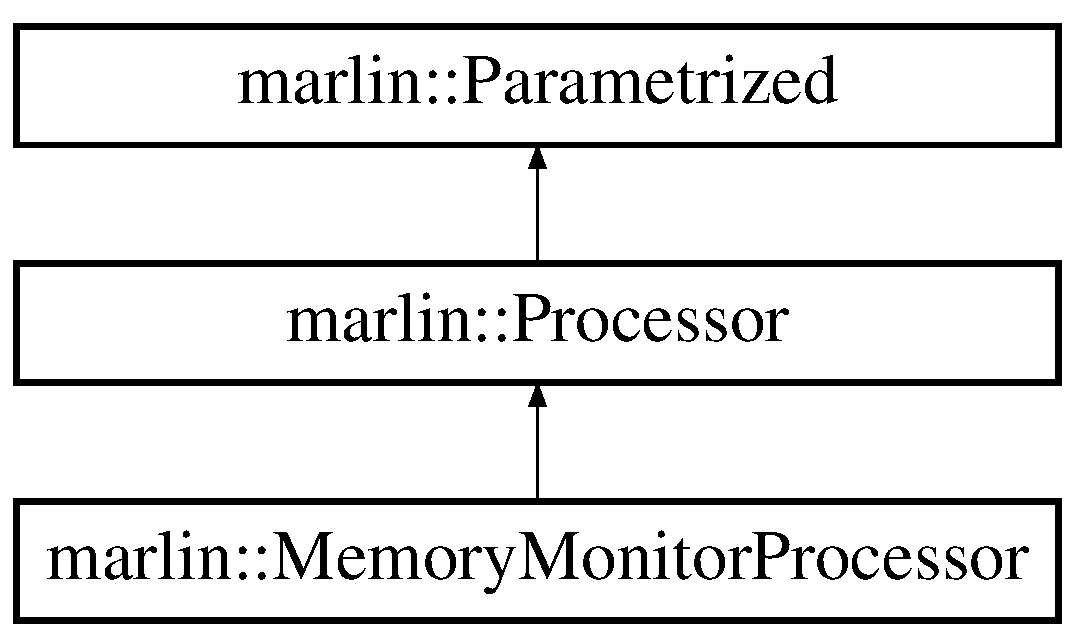
\includegraphics[height=3.000000cm]{classmarlin_1_1MemoryMonitorProcessor}
\end{center}
\end{figure}
\subsection*{Public Member Functions}
\begin{DoxyCompactItemize}
\item 
\mbox{\label{classmarlin_1_1MemoryMonitorProcessor_a866f3f0873222ad4d98cb32f88422b11}} 
\textbf{ Memory\+Monitor\+Processor} ()
\begin{DoxyCompactList}\small\item\em Constructor. \end{DoxyCompactList}\item 
\mbox{\label{classmarlin_1_1MemoryMonitorProcessor_aed420548ce070d0bdbe92f2fae9cfc17}} 
\textbf{ Processor} $\ast$ \textbf{ new\+Processor} ()
\begin{DoxyCompactList}\small\item\em Return a new instance of the processor (factory method) \end{DoxyCompactList}\item 
void \textbf{ init} ()
\begin{DoxyCompactList}\small\item\em Initialize the processor. \end{DoxyCompactList}\item 
void \textbf{ process\+Event} (E\+V\+E\+N\+T\+::\+L\+C\+Event $\ast$evt)
\begin{DoxyCompactList}\small\item\em Process an input event. \end{DoxyCompactList}\end{DoxyCompactItemize}
\subsection*{Protected Attributes}
\begin{DoxyCompactItemize}
\item 
int \textbf{ \+\_\+how\+Often} \{1\}
\begin{DoxyCompactList}\small\item\em $<$ Print event number every N events \end{DoxyCompactList}\item 
\mbox{\label{classmarlin_1_1MemoryMonitorProcessor_a6379a27ccf92de2c879860fc005d27f8}} 
unsigned int {\bfseries \+\_\+event\+Number} \{0\}
\end{DoxyCompactItemize}
\subsection*{Additional Inherited Members}


\subsection{Detailed Description}
\doxyref{Memory\+Monitor\+Processor}{p.}{classmarlin_1_1MemoryMonitorProcessor} is a memory monitoring application for Marlin. 

\subparagraph*{Input -\/ Prerequisites}

No input needed for this processor.

\subparagraph*{Output}

none


\begin{DoxyParams}{Parameters}
{\em how\+Often} & prints memory consumption every \textquotesingle{}how\+Often\textquotesingle{} events\\
\hline
\end{DoxyParams}
\begin{DoxyAuthor}{Author}
N. Nikiforou, C\+E\+RN, 
\end{DoxyAuthor}


\subsection{Member Function Documentation}
\mbox{\label{classmarlin_1_1MemoryMonitorProcessor_aa7d3b4ce08bfd0a5cd44c2ce39b8f76e}} 
\index{marlin\+::\+Memory\+Monitor\+Processor@{marlin\+::\+Memory\+Monitor\+Processor}!init@{init}}
\index{init@{init}!marlin\+::\+Memory\+Monitor\+Processor@{marlin\+::\+Memory\+Monitor\+Processor}}
\subsubsection{init()}
{\footnotesize\ttfamily void marlin\+::\+Memory\+Monitor\+Processor\+::init (\begin{DoxyParamCaption}{ }\end{DoxyParamCaption})\hspace{0.3cm}{\ttfamily [virtual]}}



Initialize the processor. 

Called at the begin of the job before anything is read. Use to initialize the processor, e.\+g. book histograms. 

Reimplemented from \textbf{ marlin\+::\+Processor} \doxyref{}{p.}{classmarlin_1_1Processor_a8194fb92a428de40ea9d891c8c8aed6b}.



References marlin\+::\+Processor\+::print\+Parameters().

\mbox{\label{classmarlin_1_1MemoryMonitorProcessor_ad1f4a9c63f04cd6a4dc1ab4ecccafa2f}} 
\index{marlin\+::\+Memory\+Monitor\+Processor@{marlin\+::\+Memory\+Monitor\+Processor}!process\+Event@{process\+Event}}
\index{process\+Event@{process\+Event}!marlin\+::\+Memory\+Monitor\+Processor@{marlin\+::\+Memory\+Monitor\+Processor}}
\subsubsection{process\+Event()}
{\footnotesize\ttfamily void marlin\+::\+Memory\+Monitor\+Processor\+::process\+Event (\begin{DoxyParamCaption}\item[{E\+V\+E\+N\+T\+::\+L\+C\+Event $\ast$}]{ }\end{DoxyParamCaption})\hspace{0.3cm}{\ttfamily [virtual]}}



Process an input event. 

Called for every event -\/ the working horse. 

Reimplemented from \textbf{ marlin\+::\+Processor} \doxyref{}{p.}{classmarlin_1_1Processor_a5bee49b5515f59fae755e0a26dfae91a}.



References \+\_\+how\+Often.



\subsection{Member Data Documentation}
\mbox{\label{classmarlin_1_1MemoryMonitorProcessor_a6540a7f87b2eb6b4ef2035b6f59fbf7d}} 
\index{marlin\+::\+Memory\+Monitor\+Processor@{marlin\+::\+Memory\+Monitor\+Processor}!\+\_\+how\+Often@{\+\_\+how\+Often}}
\index{\+\_\+how\+Often@{\+\_\+how\+Often}!marlin\+::\+Memory\+Monitor\+Processor@{marlin\+::\+Memory\+Monitor\+Processor}}
\subsubsection{\+\_\+how\+Often}
{\footnotesize\ttfamily int marlin\+::\+Memory\+Monitor\+Processor\+::\+\_\+how\+Often \{1\}\hspace{0.3cm}{\ttfamily [protected]}}



$<$ Print event number every N events 

Event counter 

Referenced by Memory\+Monitor\+Processor(), and process\+Event().



The documentation for this class was generated from the following file\+:\begin{DoxyCompactItemize}
\item 
Memory\+Monitor\+Processor.\+cc\end{DoxyCompactItemize}

\section{marlin\+:\+:Parameter Class Reference}
\label{classmarlin_1_1Parameter}\index{marlin\+::\+Parameter@{marlin\+::\+Parameter}}


\doxyref{Parameter}{p.}{classmarlin_1_1Parameter} class.  




{\ttfamily \#include $<$Parameter.\+h$>$}

Inheritance diagram for marlin\+:\+:Parameter\+:\begin{figure}[H]
\begin{center}
\leavevmode
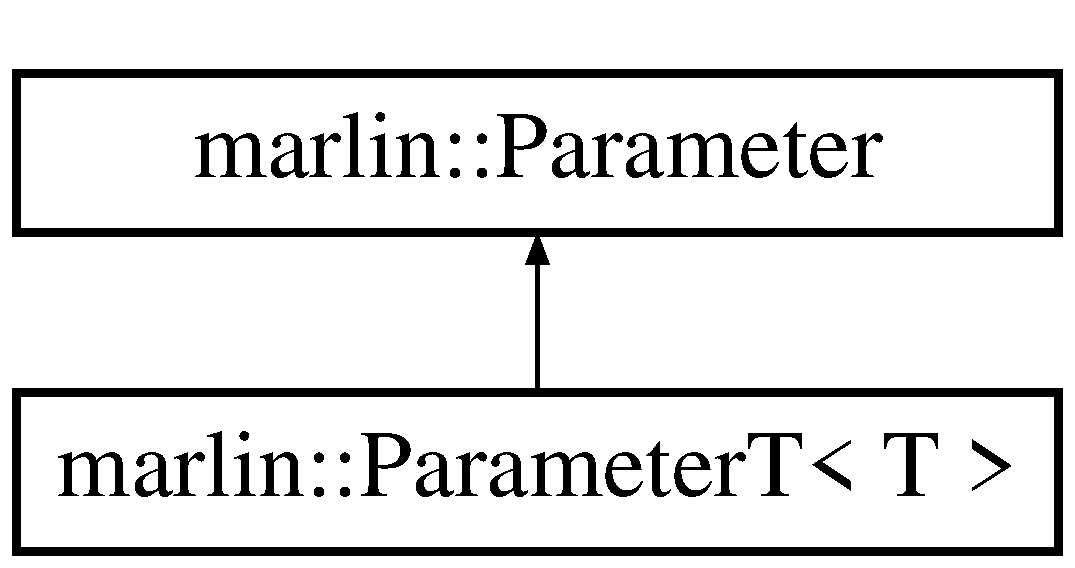
\includegraphics[height=2.000000cm]{classmarlin_1_1Parameter}
\end{center}
\end{figure}
\subsection*{Public Member Functions}
\begin{DoxyCompactItemize}
\item 
\mbox{\label{classmarlin_1_1Parameter_add0fdd82b06cc448f6b50686a16688e3}} 
const std\+::string \& \textbf{ name} () const
\begin{DoxyCompactList}\small\item\em Get the parameter name. \end{DoxyCompactList}\item 
\mbox{\label{classmarlin_1_1Parameter_a557de88ed210a1da18195376a5e2257e}} 
const std\+::string \& \textbf{ description} () const
\begin{DoxyCompactList}\small\item\em Get the parameter description. \end{DoxyCompactList}\item 
\mbox{\label{classmarlin_1_1Parameter_a90e532054f5793b8ec38727ca598b1a9}} 
int \textbf{ set\+Size} () const
\begin{DoxyCompactList}\small\item\em Get the set size (if the parameter is a vector) \end{DoxyCompactList}\item 
\mbox{\label{classmarlin_1_1Parameter_a37356534d500268e011ba6bc6e095257}} 
bool \textbf{ is\+Optional} () const
\begin{DoxyCompactList}\small\item\em Whether the parameter is optional. \end{DoxyCompactList}\item 
\mbox{\label{classmarlin_1_1Parameter_aae9c894fc3725269a444d8527a5b2585}} 
bool \textbf{ value\+Set} () const
\begin{DoxyCompactList}\small\item\em Whether the value has been set during steering file parsing. \end{DoxyCompactList}\item 
\mbox{\label{classmarlin_1_1Parameter_aa1a9dd13c74a7d42899cf334cdfcd00c}} 
virtual const std\+::string \textbf{ type} () const =0
\begin{DoxyCompactList}\small\item\em Get the parameter type as string. \end{DoxyCompactList}\item 
\mbox{\label{classmarlin_1_1Parameter_aca3d0bd4d2941c798295b557e1678875}} 
virtual const std\+::string \textbf{ value} () const =0
\begin{DoxyCompactList}\small\item\em Get the parameter value as string. \end{DoxyCompactList}\item 
\mbox{\label{classmarlin_1_1Parameter_a55c1c68f505cb90df9b020987332e63b}} 
virtual const std\+::string \textbf{ default\+Value} () const =0
\begin{DoxyCompactList}\small\item\em Get the parameter default value. \end{DoxyCompactList}\item 
virtual void \textbf{ set\+Value} (\textbf{ String\+Parameters} $\ast$params)=0
\begin{DoxyCompactList}\small\item\em Set the value using the string parameters. \end{DoxyCompactList}\end{DoxyCompactItemize}
\subsection*{Protected Attributes}
\begin{DoxyCompactItemize}
\item 
\mbox{\label{classmarlin_1_1Parameter_a232ac4d45f3eadec1ee0b8e5b690e2d0}} 
std\+::string \textbf{ \+\_\+description} \{\char`\"{}\char`\"{}\}
\begin{DoxyCompactList}\small\item\em The parameter description. \end{DoxyCompactList}\item 
\mbox{\label{classmarlin_1_1Parameter_af273f4a5651b82bd65cfe6575959a5eb}} 
std\+::string \textbf{ \+\_\+name} \{\char`\"{}\char`\"{}\}
\begin{DoxyCompactList}\small\item\em The parameter name. \end{DoxyCompactList}\item 
\mbox{\label{classmarlin_1_1Parameter_ab9023827d10c745ab66d737d4c6dd726}} 
int \textbf{ \+\_\+set\+Size} \{0\}
\begin{DoxyCompactList}\small\item\em The set size, if the parameter type is vector. \end{DoxyCompactList}\item 
\mbox{\label{classmarlin_1_1Parameter_a746762ef64f46f5712c3123d381d8dd9}} 
bool \textbf{ \+\_\+optional} \{false\}
\begin{DoxyCompactList}\small\item\em Whether the parameter is optional. \end{DoxyCompactList}\item 
\mbox{\label{classmarlin_1_1Parameter_ac1741f10bea1c9b7f9013b3ab40a1d87}} 
bool \textbf{ \+\_\+value\+Set} \{false\}
\begin{DoxyCompactList}\small\item\em Whether the value has been set after parsing. \end{DoxyCompactList}\end{DoxyCompactItemize}
\subsection*{Friends}
\begin{DoxyCompactItemize}
\item 
\mbox{\label{classmarlin_1_1Parameter_ad395c5bad5eb41cc7d1e64204857d17a}} 
std\+::ostream \& {\bfseries operator$<$$<$} (std\+::ostream \&, \textbf{ Parameter} \&)
\end{DoxyCompactItemize}


\subsection{Detailed Description}
\doxyref{Parameter}{p.}{classmarlin_1_1Parameter} class. 

Holds a steering variable.

\begin{DoxyAuthor}{Author}
F. Gaede, D\+E\+SY 

R. Ete, D\+E\+SY 
\end{DoxyAuthor}


\subsection{Member Function Documentation}
\mbox{\label{classmarlin_1_1Parameter_ad496a7fa87f2c576e60c06b183ce94af}} 
\index{marlin\+::\+Parameter@{marlin\+::\+Parameter}!set\+Value@{set\+Value}}
\index{set\+Value@{set\+Value}!marlin\+::\+Parameter@{marlin\+::\+Parameter}}
\subsubsection{set\+Value()}
{\footnotesize\ttfamily virtual void marlin\+::\+Parameter\+::set\+Value (\begin{DoxyParamCaption}\item[{\textbf{ String\+Parameters} $\ast$}]{params }\end{DoxyParamCaption})\hspace{0.3cm}{\ttfamily [pure virtual]}}



Set the value using the string parameters. 


\begin{DoxyParams}{Parameters}
{\em params} & the string parameters to get the parameter value from \\
\hline
\end{DoxyParams}


Implemented in \textbf{ marlin\+::\+Parameter\+T$<$ T $>$} \doxyref{}{p.}{classmarlin_1_1ParameterT_ae8c6cba13ed4e29b89d209bc78d40872}.



The documentation for this class was generated from the following files\+:\begin{DoxyCompactItemize}
\item 
Parameter.\+h\item 
Parameter.\+cc\end{DoxyCompactItemize}

\section{marlin\+:\+:ParameterT$<$ T $>$ Class Template Reference}
\label{classmarlin_1_1ParameterT}\index{marlin\+::\+Parameter\+T$<$ T $>$@{marlin\+::\+Parameter\+T$<$ T $>$}}


\doxyref{ParameterT}{p.}{classmarlin_1_1ParameterT} template class.  




{\ttfamily \#include $<$Parameter.\+h$>$}

Inheritance diagram for marlin\+:\+:ParameterT$<$ T $>$\+:\begin{figure}[H]
\begin{center}
\leavevmode
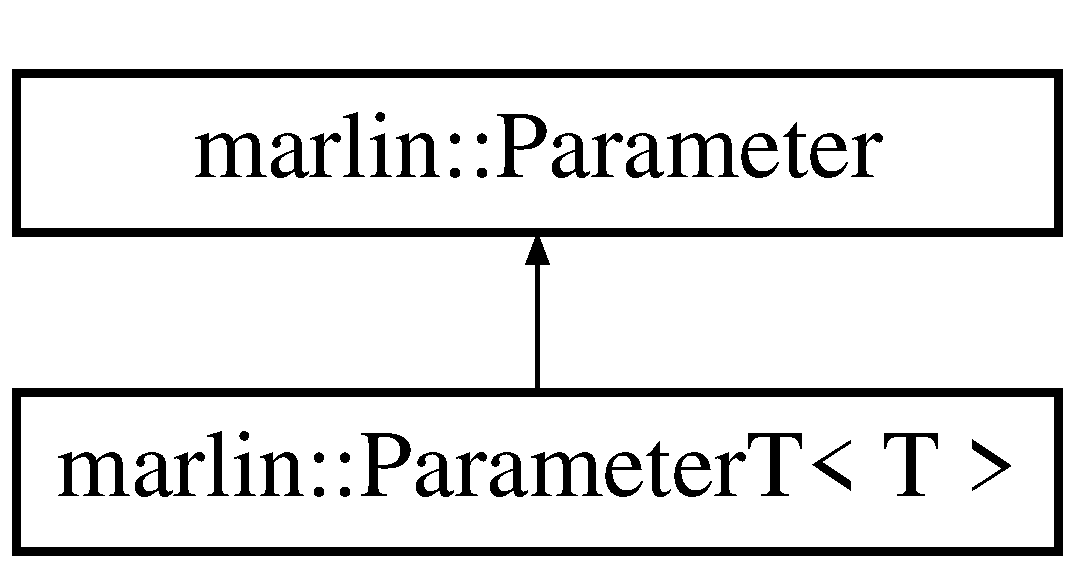
\includegraphics[height=2.000000cm]{classmarlin_1_1ParameterT}
\end{center}
\end{figure}
\subsection*{Public Member Functions}
\begin{DoxyCompactItemize}
\item 
\textbf{ ParameterT} (const std\+::string \&parameter\+Name, const std\+::string \&parameter\+Description, T \&parameter, const T \&parameter\+Default\+Value, bool optional, int parameter\+Set\+Size=0)
\begin{DoxyCompactList}\small\item\em Constructor. \end{DoxyCompactList}\item 
\mbox{\label{classmarlin_1_1ParameterT_ae1ec6d1265286ab3d22f706b94ce7e4d}} 
const T \& \textbf{ valueT} () const
\begin{DoxyCompactList}\small\item\em Get the parameter value. \end{DoxyCompactList}\item 
\mbox{\label{classmarlin_1_1ParameterT_a887a9af4990127cea332b3c581052aee}} 
const T \& \textbf{ default\+ValueT} () const
\begin{DoxyCompactList}\small\item\em Get the parameter default value. \end{DoxyCompactList}\item 
\mbox{\label{classmarlin_1_1ParameterT_a2ceaf2e914ab37dd76de70081cd4db94}} 
const std\+::string \textbf{ type} () const override
\begin{DoxyCompactList}\small\item\em Get the parameter type as string. \end{DoxyCompactList}\item 
\mbox{\label{classmarlin_1_1ParameterT_ac8dfbd4d1e1cbbfe0a005cc7877dcda8}} 
const std\+::string \textbf{ default\+Value} () const override
\begin{DoxyCompactList}\small\item\em Get the parameter default value. \end{DoxyCompactList}\item 
\mbox{\label{classmarlin_1_1ParameterT_a1ec2b70acb1805d6ac21ad3b8acaa7b4}} 
const std\+::string \textbf{ value} () const override
\begin{DoxyCompactList}\small\item\em Get the parameter value as string. \end{DoxyCompactList}\item 
void \textbf{ set\+Value} (\textbf{ String\+Parameters} $\ast$params) override
\begin{DoxyCompactList}\small\item\em Set the value using the string parameters. \end{DoxyCompactList}\end{DoxyCompactItemize}
\subsection*{Protected Attributes}
\begin{DoxyCompactItemize}
\item 
\mbox{\label{classmarlin_1_1ParameterT_af787a95b2abbe0f7fcb295e07e23dae5}} 
T \& \textbf{ \+\_\+value}
\begin{DoxyCompactList}\small\item\em The parameter value reference. \end{DoxyCompactList}\item 
\mbox{\label{classmarlin_1_1ParameterT_a1e84477db0f227f33802f2636557e63f}} 
T \textbf{ \+\_\+default\+Value}
\begin{DoxyCompactList}\small\item\em The default parameter value reference. \end{DoxyCompactList}\end{DoxyCompactItemize}


\subsection{Detailed Description}
\subsubsection*{template$<$typename T$>$\newline
class marlin\+::\+Parameter\+T$<$ T $>$}

\doxyref{ParameterT}{p.}{classmarlin_1_1ParameterT} template class. 

Templated implementation of \doxyref{Parameter}{p.}{classmarlin_1_1Parameter} class. 

\subsection{Constructor \& Destructor Documentation}
\mbox{\label{classmarlin_1_1ParameterT_aabc6b6c14504c2245aa5e58a7fb8a61a}} 
\index{marlin\+::\+ParameterT@{marlin\+::\+ParameterT}!ParameterT@{ParameterT}}
\index{ParameterT@{ParameterT}!marlin\+::\+ParameterT@{marlin\+::\+ParameterT}}
\subsubsection{Parameter\+T()}
{\footnotesize\ttfamily template$<$typename T $>$ \\
\textbf{ marlin\+::\+ParameterT}$<$ T $>$\+::\textbf{ ParameterT} (\begin{DoxyParamCaption}\item[{const std\+::string \&}]{parameter\+Name,  }\item[{const std\+::string \&}]{parameter\+Description,  }\item[{T \&}]{parameter,  }\item[{const T \&}]{parameter\+Default\+Value,  }\item[{bool}]{optional,  }\item[{int}]{parameter\+Set\+Size = {\ttfamily 0} }\end{DoxyParamCaption})\hspace{0.3cm}{\ttfamily [inline]}}



Constructor. 


\begin{DoxyParams}{Parameters}
{\em parameter\+Name} & the parameter name \\
\hline
{\em parameter\+Description} & the parameter description \\
\hline
{\em parameter} & the parameter value reference \\
\hline
{\em parameter\+Default\+Value} & the parameter default value \\
\hline
{\em optional} & whether the parameter is optional while parsing the steering file \\
\hline
{\em parameter\+Set\+Size} & the set size of the parameter, if of type vector \\
\hline
\end{DoxyParams}


References marlin\+::\+Parameter\+::\+\_\+description, marlin\+::\+Parameter\+::\+\_\+name, marlin\+::\+Parameter\+::\+\_\+optional, marlin\+::\+Parameter\+::\+\_\+set\+Size, marlin\+::\+Parameter\+T$<$ T $>$\+::\+\_\+value, and marlin\+::\+Parameter\+::\+\_\+value\+Set.



\subsection{Member Function Documentation}
\mbox{\label{classmarlin_1_1ParameterT_ae8c6cba13ed4e29b89d209bc78d40872}} 
\index{marlin\+::\+ParameterT@{marlin\+::\+ParameterT}!set\+Value@{set\+Value}}
\index{set\+Value@{set\+Value}!marlin\+::\+ParameterT@{marlin\+::\+ParameterT}}
\subsubsection{set\+Value()}
{\footnotesize\ttfamily template$<$typename T $>$ \\
void \textbf{ marlin\+::\+ParameterT}$<$ T $>$\+::set\+Value (\begin{DoxyParamCaption}\item[{\textbf{ String\+Parameters} $\ast$}]{params }\end{DoxyParamCaption})\hspace{0.3cm}{\ttfamily [override]}, {\ttfamily [virtual]}}



Set the value using the string parameters. 


\begin{DoxyParams}{Parameters}
{\em params} & the string parameters to get the parameter value from \\
\hline
\end{DoxyParams}


Implements \textbf{ marlin\+::\+Parameter} \doxyref{}{p.}{classmarlin_1_1Parameter_ad496a7fa87f2c576e60c06b183ce94af}.



References marlin\+::\+Parameter\+T$<$ T $>$\+::\+\_\+value, marlin\+::\+Parameter\+::\+\_\+value\+Set, marlin\+::\+String\+Parameters\+::get(), marlin\+::\+String\+Parameters\+::is\+Parameter\+Set(), and marlin\+::\+Parameter\+::name().



The documentation for this class was generated from the following file\+:\begin{DoxyCompactItemize}
\item 
Parameter.\+h\end{DoxyCompactItemize}

\section{marlin\+:\+:Parametrized Class Reference}
\label{classmarlin_1_1Parametrized}\index{marlin\+::\+Parametrized@{marlin\+::\+Parametrized}}
Inheritance diagram for marlin\+:\+:Parametrized\+:\begin{figure}[H]
\begin{center}
\leavevmode
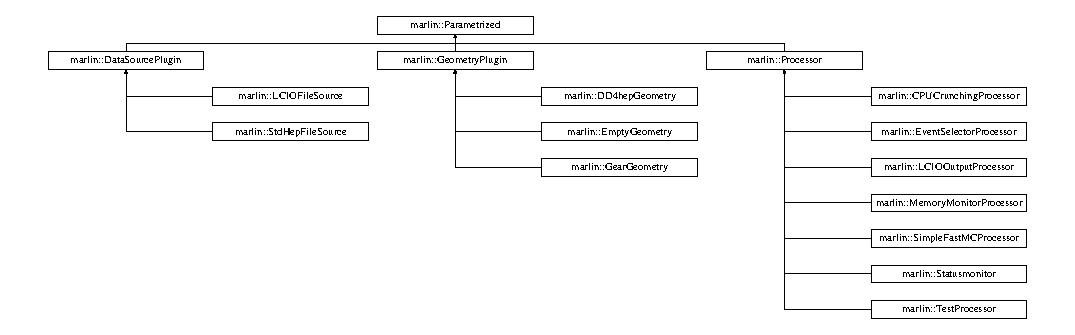
\includegraphics[height=4.057971cm]{classmarlin_1_1Parametrized}
\end{center}
\end{figure}
\subsection*{Public Types}
\begin{DoxyCompactItemize}
\item 
\mbox{\label{classmarlin_1_1Parametrized_a7e44e5f8ad96aa69ed4c6d8beb38dde7}} 
typedef std\+::shared\+\_\+ptr$<$ \textbf{ Parameter} $>$ {\bfseries Parameter\+Ptr}
\item 
\mbox{\label{classmarlin_1_1Parametrized_a1f4d3aa2858d0c28c174699e32e23e09}} 
typedef std\+::map$<$ std\+::string, Parameter\+Ptr $>$ {\bfseries Parameter\+Map}
\item 
\mbox{\label{classmarlin_1_1Parametrized_ae29f5e5170556c89e627ccda0ffc3948}} 
typedef std\+::map$<$ std\+::string, std\+::string $>$ {\bfseries L\+C\+I\+O\+Type\+Map}
\item 
\mbox{\label{classmarlin_1_1Parametrized_ace720ac8a6f7444ef5e2587cbc71b339}} 
typedef Parameter\+Map\+::iterator {\bfseries iterator}
\item 
\mbox{\label{classmarlin_1_1Parametrized_aa2acea26618105c924df2a17913035f9}} 
typedef Parameter\+Map\+::const\+\_\+iterator {\bfseries const\+\_\+iterator}
\end{DoxyCompactItemize}
\subsection*{Public Member Functions}
\begin{DoxyCompactItemize}
\item 
\mbox{\label{classmarlin_1_1Parametrized_a92848a36098a3b07bfe61c504837c927}} 
{\bfseries Parametrized} (const \textbf{ Parametrized} \&)=delete
\item 
\mbox{\label{classmarlin_1_1Parametrized_aa0bc8559aff223df77c59d21b161a270}} 
\textbf{ Parametrized} \& {\bfseries operator=} (const \textbf{ Parametrized} \&)=delete
\item 
{\footnotesize template$<$class T $>$ }\\void \textbf{ register\+Parameter} (const std\+::string \&parameter\+Name, const std\+::string \&parameter\+Description, T \&parameter, const T \&default\+Val, int set\+Size=0)
\begin{DoxyCompactList}\small\item\em Register a steering variable. \end{DoxyCompactList}\item 
{\footnotesize template$<$class T $>$ }\\void \textbf{ register\+Optional\+Parameter} (const std\+::string \&parameter\+Name, const std\+::string \&parameter\+Description, T \&parameter, const T \&default\+Val, int set\+Size=0)
\begin{DoxyCompactList}\small\item\em Same as register\+Parameter except that the parameter is optional. \end{DoxyCompactList}\item 
\mbox{\label{classmarlin_1_1Parametrized_af6546dee2f8673688677a42e2290381a}} 
void \textbf{ register\+Input\+Collection} (const std\+::string \&collection\+Type, const std\+::string \&parameter\+Name, const std\+::string \&parameter\+Description, std\+::string \&parameter, const std\+::string \&default\+Val, int set\+Size=0)
\begin{DoxyCompactList}\small\item\em Specialization of \doxyref{register\+Parameter()}{p.}{classmarlin_1_1Parametrized_a0ca3ad605ee4535cd98d2dd861c99fc3} for a parameter that defines an input collection -\/ can be used fo checking the consistency of the steering file. \end{DoxyCompactList}\item 
\mbox{\label{classmarlin_1_1Parametrized_aad86edee8d20a9e480557326f2723bf8}} 
void \textbf{ register\+Input\+Collections} (const std\+::string \&collection\+Type, const std\+::string \&parameter\+Name, const std\+::string \&parameter\+Description, std\+::vector$<$ std\+::string $>$ \&parameter, const std\+::vector$<$ std\+::string $>$ \&default\+Val, int set\+Size=0)
\begin{DoxyCompactList}\small\item\em Specialization of \doxyref{register\+Parameter()}{p.}{classmarlin_1_1Parametrized_a0ca3ad605ee4535cd98d2dd861c99fc3} for a parameter that defines one or several input collections -\/ can be used fo checking the consistency of the steering file. \end{DoxyCompactList}\item 
\mbox{\label{classmarlin_1_1Parametrized_a0d3f93922a7e4b51eb58d70e73c98e0a}} 
void \textbf{ register\+Output\+Collection} (const std\+::string \&collection\+Type, const std\+::string \&parameter\+Name, const std\+::string \&parameter\+Description, std\+::string \&parameter, const std\+::string \&default\+Val, int set\+Size=0)
\begin{DoxyCompactList}\small\item\em Specialization of \doxyref{register\+Parameter()}{p.}{classmarlin_1_1Parametrized_a0ca3ad605ee4535cd98d2dd861c99fc3} for a parameter that defines an output collection -\/ can be used fo checking the consistency of the steering file. \end{DoxyCompactList}\item 
\mbox{\label{classmarlin_1_1Parametrized_a8a0d19d32c4db1b2d12f3aa34668ce32}} 
bool \textbf{ parameter\+Set} (const std\+::string \&name)
\begin{DoxyCompactList}\small\item\em Tests whether the parameter has been set in the steering file. \end{DoxyCompactList}\item 
\mbox{\label{classmarlin_1_1Parametrized_aed2440e7fe755c79481d246dbd1e613d}} 
void \textbf{ clear\+Parameters} ()
\begin{DoxyCompactList}\small\item\em Clear the parameter map. \end{DoxyCompactList}\item 
void \textbf{ set\+Parameters} (std\+::shared\+\_\+ptr$<$ \textbf{ String\+Parameters} $>$ parameters)
\begin{DoxyCompactList}\small\item\em Update the parameter map with the input parameters. \end{DoxyCompactList}\item 
\mbox{\label{classmarlin_1_1Parametrized_a9650c1fb7ceda93f6132ac134e5a575d}} 
std\+::vector$<$ std\+::string $>$ \textbf{ parameter\+Names} () const
\begin{DoxyCompactList}\small\item\em Get the list of parameter names. \end{DoxyCompactList}\item 
{\footnotesize template$<$typename T $>$ }\\T \textbf{ get\+Parameter} (const std\+::string \&name) const
\begin{DoxyCompactList}\small\item\em Get a parameter value. \end{DoxyCompactList}\item 
\mbox{\label{classmarlin_1_1Parametrized_a97b4c36ff7fe69c82992d02e920ec1e4}} 
std\+::string \textbf{ get\+L\+C\+I\+O\+In\+Type} (const std\+::string \&col\+Name) const
\begin{DoxyCompactList}\small\item\em Return the L\+C\+IO input type for the collection col\+Name -\/ empty string if col\+Name is not a registered collection name. \end{DoxyCompactList}\item 
\mbox{\label{classmarlin_1_1Parametrized_aeb6651841982821e73262a5bca0bbeb5}} 
std\+::string \textbf{ get\+L\+C\+I\+O\+Out\+Type} (const std\+::string \&col\+Name) const
\begin{DoxyCompactList}\small\item\em Return the L\+C\+IO output type for the collection col\+Name -\/ empty string if col\+Name is not a registered collection name. \end{DoxyCompactList}\item 
bool \textbf{ is\+Input\+Collection\+Name} (const std\+::string \&parameter\+Name) const
\begin{DoxyCompactList}\small\item\em True if the given parameter defines an L\+C\+IO input collection, i.\+e. \end{DoxyCompactList}\item 
\mbox{\label{classmarlin_1_1Parametrized_ae7e2d46e9789313d1f0278e792df59a8}} 
bool \textbf{ is\+Output\+Collection\+Name} (const std\+::string \&parameter\+Name) const
\begin{DoxyCompactList}\small\item\em True if the given parameter defines an L\+C\+IO output collection. \end{DoxyCompactList}\item 
\mbox{\label{classmarlin_1_1Parametrized_adea8de32e6464b55c8f65abcadcd2cf0}} 
iterator \textbf{ pbegin} ()
\begin{DoxyCompactList}\small\item\em Begin iterator to parameter map. \end{DoxyCompactList}\item 
\mbox{\label{classmarlin_1_1Parametrized_a555eabe87c17af8711602c830661eff8}} 
iterator \textbf{ pend} ()
\begin{DoxyCompactList}\small\item\em End iterator of parameter map. \end{DoxyCompactList}\item 
\mbox{\label{classmarlin_1_1Parametrized_a826e4f088048827ddee76af63e510bf6}} 
const\+\_\+iterator \textbf{ pbegin} () const
\begin{DoxyCompactList}\small\item\em Begin iterator to parameter map. \end{DoxyCompactList}\item 
\mbox{\label{classmarlin_1_1Parametrized_a450d68c405b69b13f80836cdfd245eaa}} 
const\+\_\+iterator \textbf{ pend} () const
\begin{DoxyCompactList}\small\item\em End iterator of parameter map. \end{DoxyCompactList}\end{DoxyCompactItemize}


\subsection{Member Function Documentation}
\mbox{\label{classmarlin_1_1Parametrized_a22769ccaee2510f1dbc9be534470c15f}} 
\index{marlin\+::\+Parametrized@{marlin\+::\+Parametrized}!get\+Parameter@{get\+Parameter}}
\index{get\+Parameter@{get\+Parameter}!marlin\+::\+Parametrized@{marlin\+::\+Parametrized}}
\subsubsection{get\+Parameter()}
{\footnotesize\ttfamily template$<$typename T $>$ \\
T marlin\+::\+Parametrized\+::get\+Parameter (\begin{DoxyParamCaption}\item[{const std\+::string \&}]{name }\end{DoxyParamCaption}) const\hspace{0.3cm}{\ttfamily [inline]}}



Get a parameter value. 

If the parameter exists, an attempt to cast the parameter type to the same type as it was registered is done. It it fails, an exception is thrown. If the parameter doesn\textquotesingle{}t exists, an exception is thrown. If the parameter exists but is not set, the default value is returned.


\begin{DoxyParams}{Parameters}
{\em name} & the parameter name \\
\hline
\end{DoxyParams}
\mbox{\label{classmarlin_1_1Parametrized_a4897f750fb36f6ecc17a04f27fb1c894}} 
\index{marlin\+::\+Parametrized@{marlin\+::\+Parametrized}!is\+Input\+Collection\+Name@{is\+Input\+Collection\+Name}}
\index{is\+Input\+Collection\+Name@{is\+Input\+Collection\+Name}!marlin\+::\+Parametrized@{marlin\+::\+Parametrized}}
\subsubsection{is\+Input\+Collection\+Name()}
{\footnotesize\ttfamily bool marlin\+::\+Parametrized\+::is\+Input\+Collection\+Name (\begin{DoxyParamCaption}\item[{const std\+::string \&}]{parameter\+Name }\end{DoxyParamCaption}) const}



True if the given parameter defines an L\+C\+IO input collection, i.\+e. 

the type has been defined with set\+L\+C\+I\+O\+In\+Type(). 

Referenced by marlin\+::\+Processor\+::print\+Description\+X\+M\+L().

\mbox{\label{classmarlin_1_1Parametrized_ab682086b30a9798e0773bc01c4fb0671}} 
\index{marlin\+::\+Parametrized@{marlin\+::\+Parametrized}!register\+Optional\+Parameter@{register\+Optional\+Parameter}}
\index{register\+Optional\+Parameter@{register\+Optional\+Parameter}!marlin\+::\+Parametrized@{marlin\+::\+Parametrized}}
\subsubsection{register\+Optional\+Parameter()}
{\footnotesize\ttfamily template$<$class T $>$ \\
void marlin\+::\+Parametrized\+::register\+Optional\+Parameter (\begin{DoxyParamCaption}\item[{const std\+::string \&}]{parameter\+Name,  }\item[{const std\+::string \&}]{parameter\+Description,  }\item[{T \&}]{parameter,  }\item[{const T \&}]{default\+Val,  }\item[{int}]{set\+Size = {\ttfamily 0} }\end{DoxyParamCaption})\hspace{0.3cm}{\ttfamily [inline]}}



Same as register\+Parameter except that the parameter is optional. 

The value of the parameter will still be set to the default value, which is used to print an example steering line. Use \doxyref{parameter\+Set()}{p.}{classmarlin_1_1Parametrized_a8a0d19d32c4db1b2d12f3aa34668ce32} to check whether it actually has been set in the steering file. 

References marlin\+::\+Parameter\+::set\+Size().



Referenced by marlin\+::\+Geometry\+Plugin\+::\+Geometry\+Plugin(), marlin\+::\+L\+C\+I\+O\+Output\+Processor\+::new\+Processor(), and marlin\+::\+Processor\+::\+Processor().

\mbox{\label{classmarlin_1_1Parametrized_a0ca3ad605ee4535cd98d2dd861c99fc3}} 
\index{marlin\+::\+Parametrized@{marlin\+::\+Parametrized}!register\+Parameter@{register\+Parameter}}
\index{register\+Parameter@{register\+Parameter}!marlin\+::\+Parametrized@{marlin\+::\+Parametrized}}
\subsubsection{register\+Parameter()}
{\footnotesize\ttfamily template$<$class T $>$ \\
void marlin\+::\+Parametrized\+::register\+Parameter (\begin{DoxyParamCaption}\item[{const std\+::string \&}]{parameter\+Name,  }\item[{const std\+::string \&}]{parameter\+Description,  }\item[{T \&}]{parameter,  }\item[{const T \&}]{default\+Val,  }\item[{int}]{set\+Size = {\ttfamily 0} }\end{DoxyParamCaption})\hspace{0.3cm}{\ttfamily [inline]}}



Register a steering variable. 

The default value has to be of the {\itshape same} type as the parameter, e.\+g. 
\begin{DoxyCode}
\textcolor{keywordtype}{float} \_cut ;
\textcolor{comment}{// ...}
registerParameter( \textcolor{stringliteral}{"Cut"}, \textcolor{stringliteral}{"cut..."}, \_cut , \textcolor{keywordtype}{float}( 3.141592 ) ) ;
\end{DoxyCode}
 as implicit conversions don\textquotesingle{}t work for templates.~\newline
 The optional parameter set\+Size is used for formating the printout of parameters. This can be used if the parameter values are expected to come in sets of fixed size. 

References marlin\+::\+Parameter\+::set\+Size().



Referenced by marlin\+::\+Processor\+::register\+Processor\+Parameter().

\mbox{\label{classmarlin_1_1Parametrized_a2d4cb5f740ab82587786cd27dcab2d46}} 
\index{marlin\+::\+Parametrized@{marlin\+::\+Parametrized}!set\+Parameters@{set\+Parameters}}
\index{set\+Parameters@{set\+Parameters}!marlin\+::\+Parametrized@{marlin\+::\+Parametrized}}
\subsubsection{set\+Parameters()}
{\footnotesize\ttfamily void marlin\+::\+Parametrized\+::set\+Parameters (\begin{DoxyParamCaption}\item[{std\+::shared\+\_\+ptr$<$ \textbf{ String\+Parameters} $>$}]{parameters }\end{DoxyParamCaption})}



Update the parameter map with the input parameters. 


\begin{DoxyParams}{Parameters}
{\em parameters} & the input parameter list \\
\hline
\end{DoxyParams}


Referenced by marlin\+::\+Data\+Source\+Plugin\+::init().



The documentation for this class was generated from the following files\+:\begin{DoxyCompactItemize}
\item 
Parameter.\+h\item 
Parameter.\+cc\end{DoxyCompactItemize}

\section{marlin\+:\+:Parse\+Exception Class Reference}
\label{classmarlin_1_1ParseException}\index{marlin\+::\+Parse\+Exception@{marlin\+::\+Parse\+Exception}}


\doxyref{Parse\+Exception}{p.}{classmarlin_1_1ParseException} used for parse errors, e.\+g.  




{\ttfamily \#include $<$Exceptions.\+h$>$}

Inheritance diagram for marlin\+:\+:Parse\+Exception\+:\begin{figure}[H]
\begin{center}
\leavevmode
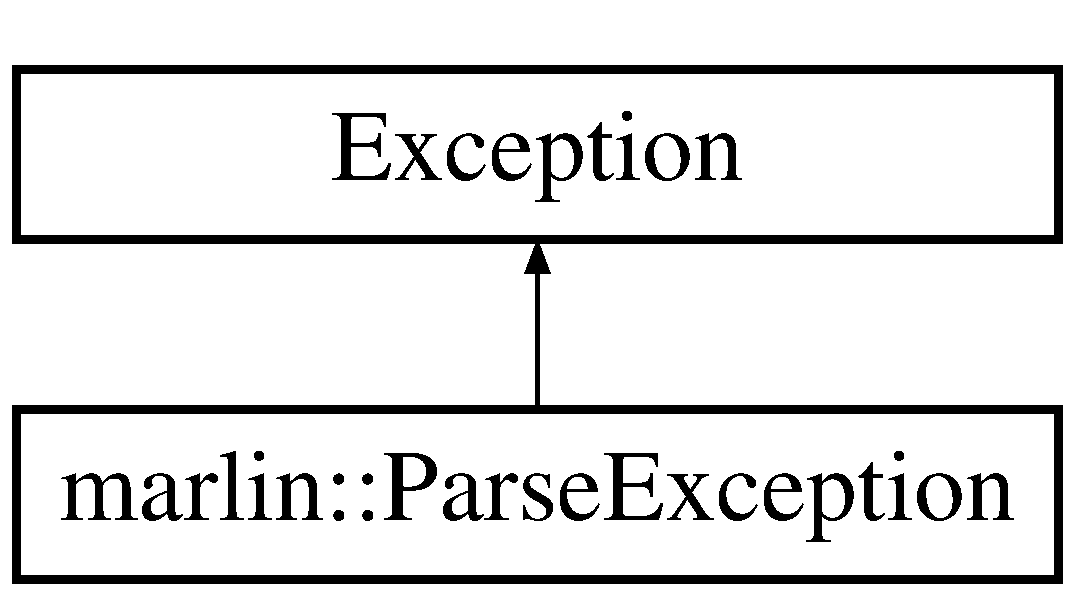
\includegraphics[height=2.000000cm]{classmarlin_1_1ParseException}
\end{center}
\end{figure}
\subsection*{Public Member Functions}
\begin{DoxyCompactItemize}
\item 
\mbox{\label{classmarlin_1_1ParseException_a4ee83450d6eb0434004ee53892dea97d}} 
{\bfseries Parse\+Exception} (const std\+::string \&text)
\end{DoxyCompactItemize}


\subsection{Detailed Description}
\doxyref{Parse\+Exception}{p.}{classmarlin_1_1ParseException} used for parse errors, e.\+g. 

when reading the steering file.

\begin{DoxyAuthor}{Author}
gaede 
\end{DoxyAuthor}
\begin{DoxyVersion}{Version}

\end{DoxyVersion}
\begin{DoxyParagraph}{Id}
\doxyref{Exceptions.\+h}{p.}{Exceptions_8h_source},v 1.\+5 2007-\/02-\/02 17\+:15\+:25 gaede Exp 
\end{DoxyParagraph}


The documentation for this class was generated from the following files\+:\begin{DoxyCompactItemize}
\item 
Exceptions.\+h\item 
Exceptions.\+cc\end{DoxyCompactItemize}

\section{marlin\+:\+:Parser Class Reference}
\label{classmarlin_1_1Parser}\index{marlin\+::\+Parser@{marlin\+::\+Parser}}


Simple parser class for Marlin.  




{\ttfamily \#include $<$Parser.\+h$>$}

Inheritance diagram for marlin\+:\+:Parser\+:\begin{figure}[H]
\begin{center}
\leavevmode
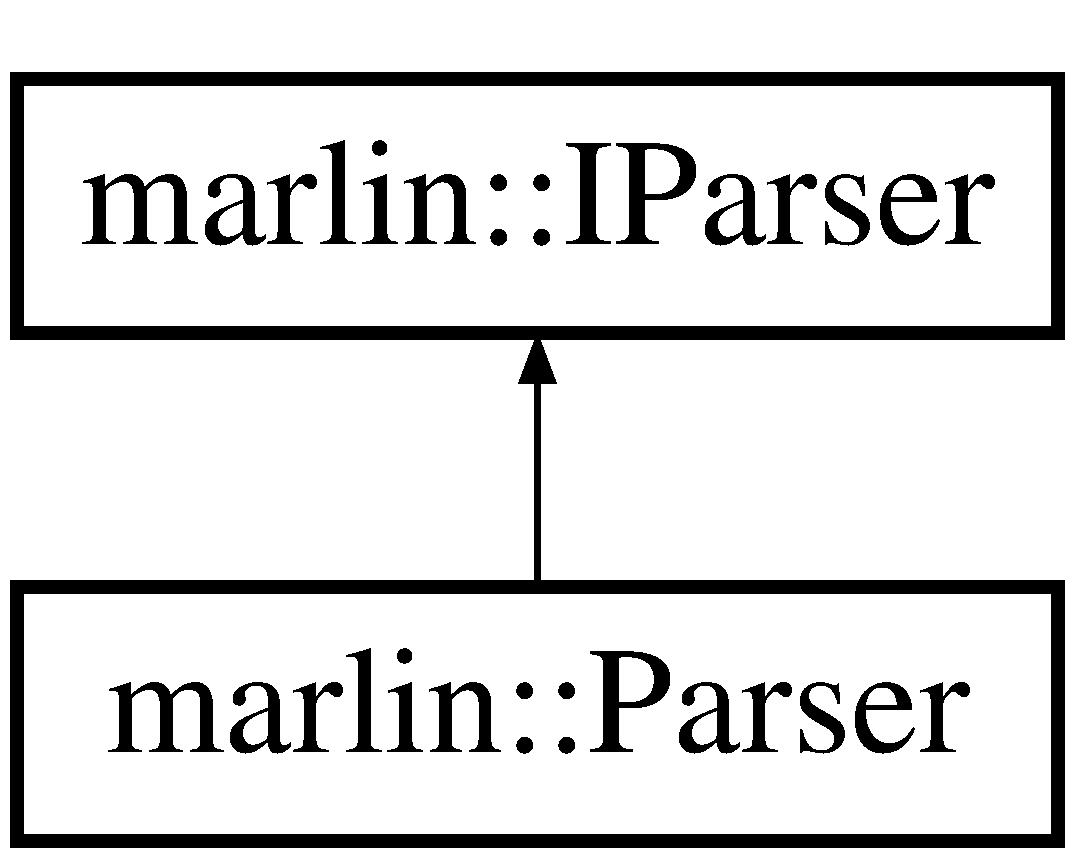
\includegraphics[height=2.000000cm]{classmarlin_1_1Parser}
\end{center}
\end{figure}
\subsection*{Public Member Functions}
\begin{DoxyCompactItemize}
\item 
\mbox{\label{classmarlin_1_1Parser_a787e9d6c02858ceb61b6ec7c09fdc56f}} 
{\bfseries Parser} (const std\+::string \&file\+Name)
\item 
\mbox{\label{classmarlin_1_1Parser_af359191c6b0c4865342fc7fe9964e359}} 
std\+::shared\+\_\+ptr$<$ \textbf{ String\+Parameters} $>$ \textbf{ get\+Parameters} (const std\+::string \&section\+Name) const
\begin{DoxyCompactList}\small\item\em Return the \doxyref{String\+Parameters}{p.}{classmarlin_1_1StringParameters} defined for this section of the steering file. \end{DoxyCompactList}\item 
\mbox{\label{classmarlin_1_1Parser_a9ad829041900bf3ac4d04898e5e4c1da}} 
void \textbf{ set\+Cmd\+Line\+Parameters} (const Command\+Line\+Parameters\+Map \&)
\begin{DoxyCompactList}\small\item\em set command line parameters \end{DoxyCompactList}\item 
\mbox{\label{classmarlin_1_1Parser_a796847899c1fbcd36edd2c4f149e19f9}} 
void \textbf{ parse} ()
\begin{DoxyCompactList}\small\item\em Parse the input file. \end{DoxyCompactList}\item 
void \textbf{ write} (const std\+::string \&fname) const
\begin{DoxyCompactList}\small\item\em Write down the parsed file in a new file. \end{DoxyCompactList}\end{DoxyCompactItemize}
\subsection*{Protected Member Functions}
\begin{DoxyCompactItemize}
\item 
\mbox{\label{classmarlin_1_1Parser_ab6bb5038a5d92c778aba06801b2baec8}} 
int \textbf{ read\+Next\+Valid\+Line} (std\+::string \&str, std\+::istream \&stream)
\begin{DoxyCompactList}\small\item\em Helper method that reads the next line from a stream that is not empty or starts with a \textquotesingle{}\#\textquotesingle{}. \end{DoxyCompactList}\end{DoxyCompactItemize}
\subsection*{Protected Attributes}
\begin{DoxyCompactItemize}
\item 
\mbox{\label{classmarlin_1_1Parser_ac9bd724f13cd1817d2c0fb3c63b68dce}} 
String\+Parameters\+Map {\bfseries \+\_\+map} \{\}
\item 
\mbox{\label{classmarlin_1_1Parser_a435303b8c025e0e4964b011699a3a5e8}} 
\textbf{ String\+Parameters} $\ast$ {\bfseries \+\_\+current}
\item 
\mbox{\label{classmarlin_1_1Parser_a104b008bdad372631fd7a9270b5dd3c2}} 
std\+::string {\bfseries \+\_\+file\+Name}
\end{DoxyCompactItemize}


\subsection{Detailed Description}
Simple parser class for Marlin. 

Creates \doxyref{Parameter}{p.}{classmarlin_1_1Parameter} objects for all sections in a steering file defined by enclosing ~\newline
 .begin Section\+Name ~\newline
 .end ~\newline
 Parameters are defined for every line that doesn\textquotesingle{}t start with \#. The first string is the name of the parameter (key) the rest of the line is interpreted as the list of values separated by whitespace. Values from multiple lines starting with the same name/key are appended to the corresponding list.

\begin{DoxyAuthor}{Author}
F. Gaede, D\+E\+SY 
\end{DoxyAuthor}
\begin{DoxyVersion}{Version}

\end{DoxyVersion}
\begin{DoxyParagraph}{Id}
\doxyref{Parser.\+h}{p.}{Parser_8h_source},v 1.\+3 2005-\/10-\/11 12\+:56\+:28 gaede Exp 
\end{DoxyParagraph}


\subsection{Member Function Documentation}
\mbox{\label{classmarlin_1_1Parser_a0eb3898c8dcd6383ccb182b0469b7737}} 
\index{marlin\+::\+Parser@{marlin\+::\+Parser}!write@{write}}
\index{write@{write}!marlin\+::\+Parser@{marlin\+::\+Parser}}
\subsubsection{write()}
{\footnotesize\ttfamily void marlin\+::\+Parser\+::write (\begin{DoxyParamCaption}\item[{const std\+::string \&}]{fname }\end{DoxyParamCaption}) const\hspace{0.3cm}{\ttfamily [virtual]}}



Write down the parsed file in a new file. 

For this implementation, just copy paste the steering file 

Implements \textbf{ marlin\+::\+I\+Parser} \doxyref{}{p.}{classmarlin_1_1IParser_aa65a00a0ce3aff902eb0e73578a5cd10}.



Referenced by set\+Cmd\+Line\+Parameters().



The documentation for this class was generated from the following files\+:\begin{DoxyCompactItemize}
\item 
Parser.\+h\item 
Parser.\+cc\end{DoxyCompactItemize}

\section{marlin\+:\+:concurrency\+:\+:P\+E\+P\+Scheduler Class Reference}
\label{classmarlin_1_1concurrency_1_1PEPScheduler}\index{marlin\+::concurrency\+::\+P\+E\+P\+Scheduler@{marlin\+::concurrency\+::\+P\+E\+P\+Scheduler}}


\doxyref{P\+E\+P\+Scheduler}{p.}{classmarlin_1_1concurrency_1_1PEPScheduler} class Parallel Event Processing Scheduler.  




{\ttfamily \#include $<$P\+E\+P\+Scheduler.\+h$>$}

Inheritance diagram for marlin\+:\+:concurrency\+:\+:P\+E\+P\+Scheduler\+:\begin{figure}[H]
\begin{center}
\leavevmode
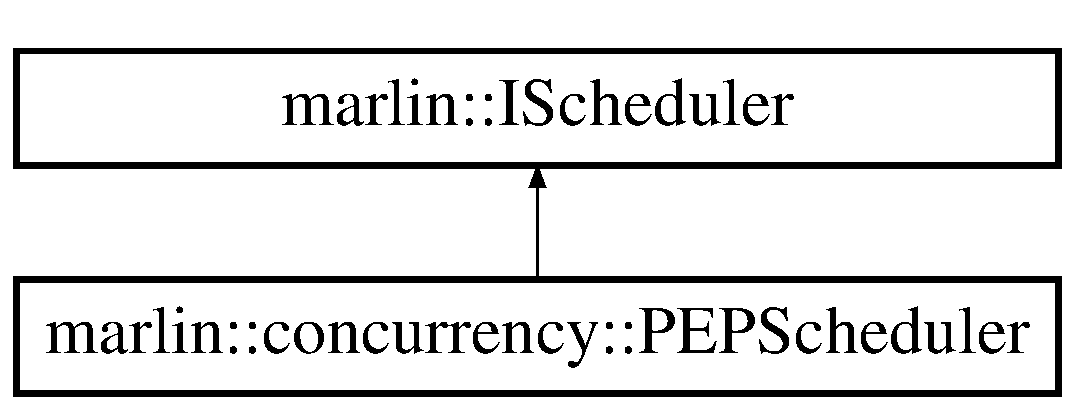
\includegraphics[height=2.000000cm]{classmarlin_1_1concurrency_1_1PEPScheduler}
\end{center}
\end{figure}
\subsection*{Public Types}
\begin{DoxyCompactItemize}
\item 
\mbox{\label{classmarlin_1_1concurrency_1_1PEPScheduler_a7bf10a5bcc0708555e45bc11aed3e550}} 
using {\bfseries Conditions\+Map} = std\+::map$<$ std\+::string, std\+::string $>$
\item 
\mbox{\label{classmarlin_1_1concurrency_1_1PEPScheduler_ad0915c5a1fd134eed88bdba3bed4d240}} 
using {\bfseries Input\+Type} = std\+::shared\+\_\+ptr$<$ E\+V\+E\+N\+T\+::\+L\+C\+Event $>$
\item 
\mbox{\label{classmarlin_1_1concurrency_1_1PEPScheduler_a15add823e8cd26547963703aeab3a7f1}} 
using {\bfseries Output\+Type} = \textbf{ Worker\+Output}
\item 
\mbox{\label{classmarlin_1_1concurrency_1_1PEPScheduler_adff02a968470f1b8e4660c03dc8b5697}} 
using {\bfseries Worker\+Pool} = \textbf{ Thread\+Pool}$<$ Input\+Type, \textbf{ Output\+Type} $>$
\item 
\mbox{\label{classmarlin_1_1concurrency_1_1PEPScheduler_a8e3289059d09315bbbd8277249b41474}} 
using {\bfseries Logger} = Logging\+::\+Logger
\item 
\mbox{\label{classmarlin_1_1concurrency_1_1PEPScheduler_aef43c2c8185becbf261dd9d26ff255eb}} 
using {\bfseries Processor\+Sequence} = std\+::shared\+\_\+ptr$<$ \textbf{ Super\+Sequence} $>$
\item 
\mbox{\label{classmarlin_1_1concurrency_1_1PEPScheduler_a03ac13bd21231a8f07e62283d0c3e2cf}} 
using {\bfseries Push\+Result\+List} = std\+::vector$<$ Worker\+Pool\+::\+Push\+Result $>$
\item 
\mbox{\label{classmarlin_1_1concurrency_1_1PEPScheduler_a408a286535499a75bb538953de9f1997}} 
using {\bfseries Event\+List} = std\+::vector$<$ std\+::shared\+\_\+ptr$<$ E\+V\+E\+N\+T\+::\+L\+C\+Event $>$ $>$
\item 
\mbox{\label{classmarlin_1_1concurrency_1_1PEPScheduler_a971c8795feda4c4920f998daccb598f1}} 
using {\bfseries Clock} = std\+::chrono\+::steady\+\_\+clock
\item 
\mbox{\label{classmarlin_1_1concurrency_1_1PEPScheduler_ada69f2fd75799a2f0b68099166fb43f1}} 
using {\bfseries Time\+Point} = std\+::chrono\+::steady\+\_\+clock\+::time\+\_\+point
\end{DoxyCompactItemize}
\subsection*{Public Member Functions}
\begin{DoxyCompactItemize}
\item 
void \textbf{ init} (\textbf{ Application} $\ast$app) override
\begin{DoxyCompactList}\small\item\em Initialize the scheduler with app parameters. \end{DoxyCompactList}\item 
\mbox{\label{classmarlin_1_1concurrency_1_1PEPScheduler_a8768321862802abd5822f476ed33b1bc}} 
void \textbf{ end} () override
\begin{DoxyCompactList}\small\item\em Terminate the scheduler activites Cleanup memory, etc ... \end{DoxyCompactList}\item 
void \textbf{ process\+Run\+Header} (std\+::shared\+\_\+ptr$<$ E\+V\+E\+N\+T\+::\+L\+C\+Run\+Header $>$ rhdr)
\begin{DoxyCompactList}\small\item\em Process a run header. \end{DoxyCompactList}\item 
void \textbf{ push\+Event} (std\+::shared\+\_\+ptr$<$ E\+V\+E\+N\+T\+::\+L\+C\+Event $>$ event) override
\begin{DoxyCompactList}\small\item\em Push a new event to the scheduler for processing. \end{DoxyCompactList}\item 
void \textbf{ pop\+Finished\+Events} (std\+::vector$<$ std\+::shared\+\_\+ptr$<$ E\+V\+E\+N\+T\+::\+L\+C\+Event $>$$>$ \&events) override
\begin{DoxyCompactList}\small\item\em Retrieve finished events from the scheduler. \end{DoxyCompactList}\item 
\mbox{\label{classmarlin_1_1concurrency_1_1PEPScheduler_aefb4fd3935440ff68c3f1e75344ead8b}} 
std\+::size\+\_\+t \textbf{ free\+Slots} () const override
\begin{DoxyCompactList}\small\item\em Get the number of free event slots. \end{DoxyCompactList}\end{DoxyCompactItemize}


\subsection{Detailed Description}
\doxyref{P\+E\+P\+Scheduler}{p.}{classmarlin_1_1concurrency_1_1PEPScheduler} class Parallel Event Processing Scheduler. 

Implements the scheduling of parallel inter-\/event processing.

A set of N worker threads are allocated at startup within a thread pool. Every time a new event is pushed in the scheduler, the event is queued in the thread pool for further processing. Note that this operation can fail if the thread pool queue is full. Use \doxyref{free\+Slots()}{p.}{classmarlin_1_1concurrency_1_1PEPScheduler_aefb4fd3935440ff68c3f1e75344ead8b} to know how many slots are free in the thread pool queue and avoid unexpected exceptions. 

\subsection{Member Function Documentation}
\mbox{\label{classmarlin_1_1concurrency_1_1PEPScheduler_a0073eec7813c50ab53aa5af128a6c774}} 
\index{marlin\+::concurrency\+::\+P\+E\+P\+Scheduler@{marlin\+::concurrency\+::\+P\+E\+P\+Scheduler}!init@{init}}
\index{init@{init}!marlin\+::concurrency\+::\+P\+E\+P\+Scheduler@{marlin\+::concurrency\+::\+P\+E\+P\+Scheduler}}
\subsubsection{init()}
{\footnotesize\ttfamily void marlin\+::concurrency\+::\+P\+E\+P\+Scheduler\+::init (\begin{DoxyParamCaption}\item[{\textbf{ Application} $\ast$}]{app }\end{DoxyParamCaption})\hspace{0.3cm}{\ttfamily [override]}, {\ttfamily [virtual]}}



Initialize the scheduler with app parameters. 


\begin{DoxyParams}{Parameters}
{\em app} & the application in which the scheduler runs \\
\hline
\end{DoxyParams}


Implements \textbf{ marlin\+::\+I\+Scheduler} \doxyref{}{p.}{classmarlin_1_1IScheduler_a043b3fac1587242d8937aaca575d0a8a}.



References marlin\+::\+Application\+::create\+Logger(), and marlin\+::clock\+::now().

\mbox{\label{classmarlin_1_1concurrency_1_1PEPScheduler_a1ea04a94fdbe98fc3c9c0802a3bff3c5}} 
\index{marlin\+::concurrency\+::\+P\+E\+P\+Scheduler@{marlin\+::concurrency\+::\+P\+E\+P\+Scheduler}!pop\+Finished\+Events@{pop\+Finished\+Events}}
\index{pop\+Finished\+Events@{pop\+Finished\+Events}!marlin\+::concurrency\+::\+P\+E\+P\+Scheduler@{marlin\+::concurrency\+::\+P\+E\+P\+Scheduler}}
\subsubsection{pop\+Finished\+Events()}
{\footnotesize\ttfamily void marlin\+::concurrency\+::\+P\+E\+P\+Scheduler\+::pop\+Finished\+Events (\begin{DoxyParamCaption}\item[{std\+::vector$<$ std\+::shared\+\_\+ptr$<$ E\+V\+E\+N\+T\+::\+L\+C\+Event $>$$>$ \&}]{events }\end{DoxyParamCaption})\hspace{0.3cm}{\ttfamily [override]}, {\ttfamily [virtual]}}



Retrieve finished events from the scheduler. 


\begin{DoxyParams}{Parameters}
{\em events} & the list of event to retrieve \\
\hline
\end{DoxyParams}


Implements \textbf{ marlin\+::\+I\+Scheduler} \doxyref{}{p.}{classmarlin_1_1IScheduler_a30b54277206eca898a0ea8ac6f44d883}.

\mbox{\label{classmarlin_1_1concurrency_1_1PEPScheduler_a83744239f6f487f3d515ec126d10096e}} 
\index{marlin\+::concurrency\+::\+P\+E\+P\+Scheduler@{marlin\+::concurrency\+::\+P\+E\+P\+Scheduler}!process\+Run\+Header@{process\+Run\+Header}}
\index{process\+Run\+Header@{process\+Run\+Header}!marlin\+::concurrency\+::\+P\+E\+P\+Scheduler@{marlin\+::concurrency\+::\+P\+E\+P\+Scheduler}}
\subsubsection{process\+Run\+Header()}
{\footnotesize\ttfamily void marlin\+::concurrency\+::\+P\+E\+P\+Scheduler\+::process\+Run\+Header (\begin{DoxyParamCaption}\item[{std\+::shared\+\_\+ptr$<$ E\+V\+E\+N\+T\+::\+L\+C\+Run\+Header $>$}]{rhdr }\end{DoxyParamCaption})\hspace{0.3cm}{\ttfamily [virtual]}}



Process a run header. 


\begin{DoxyParams}{Parameters}
{\em rhdr} & the run header to process \\
\hline
\end{DoxyParams}


Implements \textbf{ marlin\+::\+I\+Scheduler} \doxyref{}{p.}{classmarlin_1_1IScheduler_a2f77a7a3b74b875bc492311f8971ff37}.



References marlin\+::clock\+::now().

\mbox{\label{classmarlin_1_1concurrency_1_1PEPScheduler_a2958256e8d5b36cb00cf0326f2c01084}} 
\index{marlin\+::concurrency\+::\+P\+E\+P\+Scheduler@{marlin\+::concurrency\+::\+P\+E\+P\+Scheduler}!push\+Event@{push\+Event}}
\index{push\+Event@{push\+Event}!marlin\+::concurrency\+::\+P\+E\+P\+Scheduler@{marlin\+::concurrency\+::\+P\+E\+P\+Scheduler}}
\subsubsection{push\+Event()}
{\footnotesize\ttfamily void marlin\+::concurrency\+::\+P\+E\+P\+Scheduler\+::push\+Event (\begin{DoxyParamCaption}\item[{std\+::shared\+\_\+ptr$<$ E\+V\+E\+N\+T\+::\+L\+C\+Event $>$}]{event }\end{DoxyParamCaption})\hspace{0.3cm}{\ttfamily [override]}, {\ttfamily [virtual]}}



Push a new event to the scheduler for processing. 


\begin{DoxyParams}{Parameters}
{\em event} & the event to push \\
\hline
\end{DoxyParams}


Implements \textbf{ marlin\+::\+I\+Scheduler} \doxyref{}{p.}{classmarlin_1_1IScheduler_a336598b4b1a9643fabcc1487944208d2}.



The documentation for this class was generated from the following files\+:\begin{DoxyCompactItemize}
\item 
P\+E\+P\+Scheduler.\+h\item 
P\+E\+P\+Scheduler.\+cc\end{DoxyCompactItemize}

\section{marlin\+:\+:Plugin\+Manager Class Reference}
\label{classmarlin_1_1PluginManager}\index{marlin\+::\+Plugin\+Manager@{marlin\+::\+Plugin\+Manager}}


\doxyref{Plugin\+Manager}{p.}{classmarlin_1_1PluginManager} singleton class Responsible for loading shared libraries and collecting processor factory instances.  




{\ttfamily \#include $<$Plugin\+Manager.\+h$>$}

\subsection*{Public Types}
\begin{DoxyCompactItemize}
\item 
\mbox{\label{classmarlin_1_1PluginManager_ad48570cd088c233a00f99a635bd4239c}} 
typedef std\+::shared\+\_\+ptr$<$ void $>$ {\bfseries Plugin\+Ptr}
\item 
\mbox{\label{classmarlin_1_1PluginManager_a3ee0e73ead8c7cf123643f287dd01f64}} 
typedef std\+::function$<$ Plugin\+Ptr()$>$ {\bfseries Factory\+Function}
\item 
\mbox{\label{classmarlin_1_1PluginManager_a71c1c15ffe8950ff59ecf433a1718f1d}} 
typedef std\+::map$<$ std\+::string, Factory\+Function $>$ {\bfseries Factory\+Map}
\item 
\mbox{\label{classmarlin_1_1PluginManager_a23181783ed967345be21fc1ef646df61}} 
typedef std\+::map$<$ Plugin\+Type, Factory\+Map $>$ {\bfseries Plugin\+Factory\+Map}
\item 
\mbox{\label{classmarlin_1_1PluginManager_a8e8e716c2e9cc49b8d5893f27cb51fc4}} 
typedef std\+::vector$<$ void $\ast$ $>$ {\bfseries Library\+List}
\item 
\mbox{\label{classmarlin_1_1PluginManager_aaa68e451e81c1c6a3ed93d0956468566}} 
typedef Logging\+::\+Logger {\bfseries Logger}
\item 
\mbox{\label{classmarlin_1_1PluginManager_a6c9ccfc74852623f407135a60d9f3a4d}} 
typedef std\+::recursive\+\_\+mutex {\bfseries mutex\+\_\+type}
\item 
\mbox{\label{classmarlin_1_1PluginManager_af7e863ba57ed78b174279d53aff52f45}} 
typedef std\+::lock\+\_\+guard$<$ mutex\+\_\+type $>$ {\bfseries lock\+\_\+type}
\end{DoxyCompactItemize}
\subsection*{Public Member Functions}
\begin{DoxyCompactItemize}
\item 
{\footnotesize template$<$typename T $>$ }\\void \textbf{ register\+Plugin} (Plugin\+Type type, const std\+::string \&name, bool ignore\+Duplicate=true)
\begin{DoxyCompactList}\small\item\em Register a new plugin to the manager. \end{DoxyCompactList}\item 
void \textbf{ register\+Plugin} (Plugin\+Type type, const std\+::string \&name, Factory\+Function factory\+Function, bool ignore\+Duplicate=true)
\begin{DoxyCompactList}\small\item\em Register a new plugin to the manager. \end{DoxyCompactList}\item 
bool \textbf{ load\+Libraries} (const std\+::string \&envvar=\char`\"{}M\+A\+R\+L\+I\+N\+\_\+\+D\+LL\char`\"{})
\begin{DoxyCompactList}\small\item\em Load shared libraries to populate the list of plugins. \end{DoxyCompactList}\item 
std\+::vector$<$ std\+::string $>$ \textbf{ plugin\+Names} (Plugin\+Type type) const
\begin{DoxyCompactList}\small\item\em Get all registered plugin name for the given type. \end{DoxyCompactList}\item 
bool \textbf{ plugin\+Registered} (Plugin\+Type type, const std\+::string \&name) const
\begin{DoxyCompactList}\small\item\em Whether the plugin of given type and name is registered. \end{DoxyCompactList}\item 
{\footnotesize template$<$typename T $>$ }\\std\+::shared\+\_\+ptr$<$ T $>$ \textbf{ create} (Plugin\+Type type, const std\+::string \&name) const
\begin{DoxyCompactList}\small\item\em Create a new plugin instance. \end{DoxyCompactList}\item 
\mbox{\label{classmarlin_1_1PluginManager_ac23d6fb4eff58932c797517efdfe4bbf}} 
void \textbf{ dump} () const
\begin{DoxyCompactList}\small\item\em Dump plugin manager content in console. \end{DoxyCompactList}\item 
\mbox{\label{classmarlin_1_1PluginManager_a9f7301e90cd1e63c4ed8feb95dfee642}} 
Logger \textbf{ logger} () const
\begin{DoxyCompactList}\small\item\em Get the plugin manager logger. \end{DoxyCompactList}\end{DoxyCompactItemize}
\subsection*{Static Public Member Functions}
\begin{DoxyCompactItemize}
\item 
\mbox{\label{classmarlin_1_1PluginManager_a70d1131b2f514ed29e8b69797c5abad4}} 
static \textbf{ Plugin\+Manager} \& \textbf{ instance} ()
\begin{DoxyCompactList}\small\item\em Get the plugin manager instance. \end{DoxyCompactList}\end{DoxyCompactItemize}


\subsection{Detailed Description}
\doxyref{Plugin\+Manager}{p.}{classmarlin_1_1PluginManager} singleton class Responsible for loading shared libraries and collecting processor factory instances. 

\doxyref{Processor}{p.}{classmarlin_1_1Processor} instances can be created from factories using the \doxyref{Plugin\+Manager\+::create()}{p.}{classmarlin_1_1PluginManager_a637d123bd1f6bd8f4bc1ae6ee33d214c} method on query. 

\subsection{Member Function Documentation}
\mbox{\label{classmarlin_1_1PluginManager_a637d123bd1f6bd8f4bc1ae6ee33d214c}} 
\index{marlin\+::\+Plugin\+Manager@{marlin\+::\+Plugin\+Manager}!create@{create}}
\index{create@{create}!marlin\+::\+Plugin\+Manager@{marlin\+::\+Plugin\+Manager}}
\subsubsection{create()}
{\footnotesize\ttfamily template$<$typename T $>$ \\
std\+::shared\+\_\+ptr$<$ T $>$ marlin\+::\+Plugin\+Manager\+::create (\begin{DoxyParamCaption}\item[{Plugin\+Type}]{type,  }\item[{const std\+::string \&}]{name }\end{DoxyParamCaption}) const\hspace{0.3cm}{\ttfamily [inline]}}



Create a new plugin instance. 

A factory function must have been registered before hand. The template parameter T is the final plugin type requested by the caller.


\begin{DoxyParams}{Parameters}
{\em type} & the plugin type \\
\hline
{\em name} & the plugin name \\
\hline
\end{DoxyParams}
\mbox{\label{classmarlin_1_1PluginManager_ad74d076f457c0df28461dd89d932eee0}} 
\index{marlin\+::\+Plugin\+Manager@{marlin\+::\+Plugin\+Manager}!load\+Libraries@{load\+Libraries}}
\index{load\+Libraries@{load\+Libraries}!marlin\+::\+Plugin\+Manager@{marlin\+::\+Plugin\+Manager}}
\subsubsection{load\+Libraries()}
{\footnotesize\ttfamily bool marlin\+::\+Plugin\+Manager\+::load\+Libraries (\begin{DoxyParamCaption}\item[{const std\+::string \&}]{envvar = {\ttfamily \char`\"{}MARLIN\+\_\+DLL\char`\"{}} }\end{DoxyParamCaption})}



Load shared libraries to populate the list of plugins. 


\begin{DoxyParams}{Parameters}
{\em envvar} & the environment variable to load the libraries from \\
\hline
\end{DoxyParams}
\mbox{\label{classmarlin_1_1PluginManager_a845d591efb847a544bf9a0d2c81bc9f3}} 
\index{marlin\+::\+Plugin\+Manager@{marlin\+::\+Plugin\+Manager}!plugin\+Names@{plugin\+Names}}
\index{plugin\+Names@{plugin\+Names}!marlin\+::\+Plugin\+Manager@{marlin\+::\+Plugin\+Manager}}
\subsubsection{plugin\+Names()}
{\footnotesize\ttfamily std\+::vector$<$ std\+::string $>$ marlin\+::\+Plugin\+Manager\+::plugin\+Names (\begin{DoxyParamCaption}\item[{Plugin\+Type}]{type }\end{DoxyParamCaption}) const}



Get all registered plugin name for the given type. 


\begin{DoxyParams}{Parameters}
{\em type} & the plugin type \\
\hline
\end{DoxyParams}
\mbox{\label{classmarlin_1_1PluginManager_a5fba86581eb9b75007f6fea095ea00a0}} 
\index{marlin\+::\+Plugin\+Manager@{marlin\+::\+Plugin\+Manager}!plugin\+Registered@{plugin\+Registered}}
\index{plugin\+Registered@{plugin\+Registered}!marlin\+::\+Plugin\+Manager@{marlin\+::\+Plugin\+Manager}}
\subsubsection{plugin\+Registered()}
{\footnotesize\ttfamily bool marlin\+::\+Plugin\+Manager\+::plugin\+Registered (\begin{DoxyParamCaption}\item[{Plugin\+Type}]{type,  }\item[{const std\+::string \&}]{name }\end{DoxyParamCaption}) const}



Whether the plugin of given type and name is registered. 


\begin{DoxyParams}{Parameters}
{\em type} & the plugin type to check \\
\hline
{\em name} & the plugin name to check \\
\hline
\end{DoxyParams}
\mbox{\label{classmarlin_1_1PluginManager_a7727b55557b222b891e99a609acc66c7}} 
\index{marlin\+::\+Plugin\+Manager@{marlin\+::\+Plugin\+Manager}!register\+Plugin@{register\+Plugin}}
\index{register\+Plugin@{register\+Plugin}!marlin\+::\+Plugin\+Manager@{marlin\+::\+Plugin\+Manager}}
\subsubsection{register\+Plugin()\hspace{0.1cm}{\footnotesize\ttfamily [1/2]}}
{\footnotesize\ttfamily template$<$typename T $>$ \\
void marlin\+::\+Plugin\+Manager\+::register\+Plugin (\begin{DoxyParamCaption}\item[{Plugin\+Type}]{type,  }\item[{const std\+::string \&}]{name,  }\item[{bool}]{ignore\+Duplicate = {\ttfamily true} }\end{DoxyParamCaption})\hspace{0.3cm}{\ttfamily [inline]}}



Register a new plugin to the manager. 

A new factory function creating an object of type T is inserted into the registry. The type T must be default constructible. If you want to provide a custom factory function, use the corresponding overloaded function. If the flag ignore\+Duplicate is set to true, no exception is thrown in case a duplicate is found in the registry. In this case, the registry is not modified.


\begin{DoxyParams}{Parameters}
{\em type} & the plugin type \\
\hline
{\em name} & the plugin name \\
\hline
{\em ignore\+Duplicate} & whether to avoid exception throw in case of duplicate entry \\
\hline
\end{DoxyParams}


Referenced by marlin\+::\+Processor\+::\+Processor().

\mbox{\label{classmarlin_1_1PluginManager_a596aff81039e87c56109da3062f2bc51}} 
\index{marlin\+::\+Plugin\+Manager@{marlin\+::\+Plugin\+Manager}!register\+Plugin@{register\+Plugin}}
\index{register\+Plugin@{register\+Plugin}!marlin\+::\+Plugin\+Manager@{marlin\+::\+Plugin\+Manager}}
\subsubsection{register\+Plugin()\hspace{0.1cm}{\footnotesize\ttfamily [2/2]}}
{\footnotesize\ttfamily void marlin\+::\+Plugin\+Manager\+::register\+Plugin (\begin{DoxyParamCaption}\item[{Plugin\+Type}]{type,  }\item[{const std\+::string \&}]{name,  }\item[{Factory\+Function}]{factory\+Function,  }\item[{bool}]{ignore\+Duplicate = {\ttfamily true} }\end{DoxyParamCaption})}



Register a new plugin to the manager. 

See overloaded function description for more details


\begin{DoxyParams}{Parameters}
{\em type} & the plugin type \\
\hline
{\em name} & the plugin name \\
\hline
{\em factory\+Function} & the factory function responsible for the plugin creation \\
\hline
{\em ignore\+Duplicate} & whether to avoid exception throw in case of duplicate entry \\
\hline
\end{DoxyParams}


The documentation for this class was generated from the following files\+:\begin{DoxyCompactItemize}
\item 
Plugin\+Manager.\+h\item 
Plugin\+Manager.\+cc\end{DoxyCompactItemize}

\section{marlin\+:\+:Processor Class Reference}
\label{classmarlin_1_1Processor}\index{marlin\+::\+Processor@{marlin\+::\+Processor}}


\doxyref{Processor}{p.}{classmarlin_1_1Processor} class.  




{\ttfamily \#include $<$Processor.\+h$>$}

Inheritance diagram for marlin\+:\+:Processor\+:\begin{figure}[H]
\begin{center}
\leavevmode
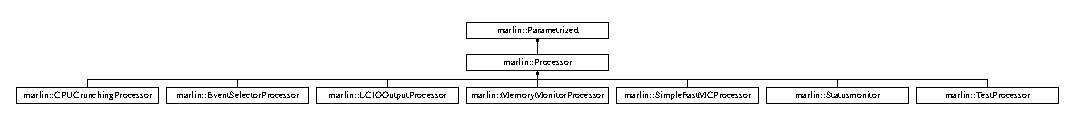
\includegraphics[height=1.159420cm]{classmarlin_1_1Processor}
\end{center}
\end{figure}
\subsection*{Public Types}
\begin{DoxyCompactItemize}
\item 
enum \textbf{ Runtime\+Option} \{ {\bfseries Critical}, 
\textbf{ Runtime\+Option\+::\+Clone}
 \}\begin{DoxyCompactList}\small\item\em Runtime\+Option enumerator. \end{DoxyCompactList}
\item 
\mbox{\label{classmarlin_1_1Processor_a7ea4ef8fdb4a2c291b2a505f96e945d3}} 
using {\bfseries Runtime\+Options} = std\+::map$<$ \textbf{ Runtime\+Option}, bool $>$
\end{DoxyCompactItemize}
\subsection*{Public Member Functions}
\begin{DoxyCompactItemize}
\item 
\textbf{ Processor} (const std\+::string \&type\+Name)
\begin{DoxyCompactList}\small\item\em Constructor. \end{DoxyCompactList}\item 
\mbox{\label{classmarlin_1_1Processor_a75ba6b66644e5273a896053df31aac4d}} 
virtual \textbf{ Processor} $\ast$ \textbf{ new\+Processor} ()=0
\begin{DoxyCompactList}\small\item\em Return a new instance of the processor (factory method) \end{DoxyCompactList}\item 
virtual void \textbf{ init} ()
\begin{DoxyCompactList}\small\item\em Initialize the processor. \end{DoxyCompactList}\item 
virtual void \textbf{ process\+Run\+Header} (E\+V\+E\+N\+T\+::\+L\+C\+Run\+Header $\ast$)
\begin{DoxyCompactList}\small\item\em Process a run header (start of run) Called for every run, e.\+g. \end{DoxyCompactList}\item 
virtual void \textbf{ process\+Event} (E\+V\+E\+N\+T\+::\+L\+C\+Event $\ast$)
\begin{DoxyCompactList}\small\item\em Process an input event. \end{DoxyCompactList}\item 
virtual void \textbf{ check} (E\+V\+E\+N\+T\+::\+L\+C\+Event $\ast$)
\begin{DoxyCompactList}\small\item\em Called for every event -\/ right after \doxyref{process\+Event()}{p.}{classmarlin_1_1Processor_a5bee49b5515f59fae755e0a26dfae91a} has been called for this processor. \end{DoxyCompactList}\item 
virtual void \textbf{ end} ()
\begin{DoxyCompactList}\small\item\em Terminate the processor. \end{DoxyCompactList}\item 
\mbox{\label{classmarlin_1_1Processor_a35f96eb55174f2cb718cb7a148aa7f92}} 
virtual const std\+::string \& \textbf{ type} () const
\begin{DoxyCompactList}\small\item\em Return type name for the processor (as set in constructor). \end{DoxyCompactList}\item 
\mbox{\label{classmarlin_1_1Processor_a86628d7158feffaa5e1559dde5a72cb9}} 
virtual const std\+::string \& \textbf{ name} () const
\begin{DoxyCompactList}\small\item\em Return the name of this processor. \end{DoxyCompactList}\item 
\mbox{\label{classmarlin_1_1Processor_afab806e3ddaa4750aadfaec08dd36fb4}} 
virtual const std\+::string \& \textbf{ log\+Level\+Name} () const
\begin{DoxyCompactList}\small\item\em Return the name of the local verbosity level of this processor -\/ \char`\"{}\char`\"{} if not set. \end{DoxyCompactList}\item 
\mbox{\label{classmarlin_1_1Processor_a40e2d0226beb00eef02b10d90b67d5c2}} 
virtual std\+::shared\+\_\+ptr$<$ \textbf{ String\+Parameters} $>$ \textbf{ parameters} () const
\begin{DoxyCompactList}\small\item\em Return the parameters defined for this \doxyref{Processor}{p.}{classmarlin_1_1Processor}. \end{DoxyCompactList}\item 
\mbox{\label{classmarlin_1_1Processor_ad1a3456636aefed5614da48ae1505e90}} 
virtual void \textbf{ print\+Description} () const
\begin{DoxyCompactList}\small\item\em Print information about this processor in A\+S\+C\+II steering file format. \end{DoxyCompactList}\item 
\mbox{\label{classmarlin_1_1Processor_a9e02bd77fda1bfae6094317c731bbf76}} 
virtual void \textbf{ print\+Description\+X\+ML} (std\+::ostream \&stream=std\+::cout) const
\begin{DoxyCompactList}\small\item\em Print information about this processor in X\+ML steering file format. \end{DoxyCompactList}\item 
\mbox{\label{classmarlin_1_1Processor_ae5c9d2f7b807eb1918865cbcfea2a3eb}} 
{\footnotesize template$<$class T $>$ }\\void \textbf{ print\+Parameters} () const
\begin{DoxyCompactList}\small\item\em Print the parameters and their values depending on the given verbosity level. \end{DoxyCompactList}\item 
\mbox{\label{classmarlin_1_1Processor_ac04b1c9bd81e0220e1061bfcb78e06b2}} 
void \textbf{ print\+Parameters} () const
\begin{DoxyCompactList}\small\item\em Print the parameters and their values with verbosity level M\+E\+S\+S\+A\+GE. \end{DoxyCompactList}\item 
\mbox{\label{classmarlin_1_1Processor_a91a0b8c0134bb7b20bd1a964fe90130b}} 
const std\+::string \& \textbf{ description} () const
\begin{DoxyCompactList}\small\item\em Description of processor. \end{DoxyCompactList}\item 
std\+::pair$<$ bool, bool $>$ \textbf{ get\+Forced\+Runtime\+Option} (\textbf{ Runtime\+Option} option) const
\begin{DoxyCompactList}\small\item\em Get the forced runtime option settings. \end{DoxyCompactList}\item 
\mbox{\label{classmarlin_1_1Processor_a1e85f5c5bad8928bedb2b1df520ee76d}} 
void \textbf{ base\+Init} (\textbf{ Application} $\ast$application)
\begin{DoxyCompactList}\small\item\em Sets the registered steering parameters before calling \doxyref{init()}{p.}{classmarlin_1_1Processor_a8194fb92a428de40ea9d891c8c8aed6b} \end{DoxyCompactList}\item 
\mbox{\label{classmarlin_1_1Processor_a545071fed6d403b15ac865df372615b1}} 
void \textbf{ set\+Parameters} (std\+::shared\+\_\+ptr$<$ \textbf{ String\+Parameters} $>$ \textbf{ parameters})
\begin{DoxyCompactList}\small\item\em Initialize the parameters. \end{DoxyCompactList}\item 
\mbox{\label{classmarlin_1_1Processor_ac2f12ef3d8d1fe42482c034778446439}} 
{\footnotesize template$<$class T $>$ }\\void {\bfseries message} (const std\+::ostream \&m) const
\end{DoxyCompactItemize}
\subsection*{Protected Member Functions}
\begin{DoxyCompactItemize}
\item 
void \textbf{ force\+Runtime\+Option} (\textbf{ Runtime\+Option} option, bool value)
\begin{DoxyCompactList}\small\item\em Force the runtime option to a given boolean value. \end{DoxyCompactList}\item 
\mbox{\label{classmarlin_1_1Processor_ac2e6decb4ba336ec5c09289bd6bc9896}} 
{\footnotesize template$<$class T $>$ }\\void \textbf{ register\+Processor\+Parameter} (const std\+::string \&parameter\+Name, const std\+::string \&parameter\+Description, T \&parameter, const T \&default\+Val, int set\+Size=0)
\begin{DoxyCompactList}\small\item\em Alias function to \doxyref{Parametrized\+::register\+Parameter}{p.}{classmarlin_1_1Parametrized_a0ca3ad605ee4535cd98d2dd861c99fc3}. \end{DoxyCompactList}\item 
{\footnotesize template$<$class T $>$ }\\void \textbf{ message} (const std\+::string \&m) const
\begin{DoxyCompactList}\small\item\em Print message according to verbosity level of the templated parameter (one of D\+E\+B\+UG, M\+E\+S\+S\+A\+GE, W\+A\+R\+N\+I\+NG, E\+R\+R\+OR ) and the global parameter \char`\"{}\+Verbosity\char`\"{}. \end{DoxyCompactList}\item 
{\footnotesize template$<$class T $>$ }\\void \textbf{ message} (const std\+::basic\+\_\+ostream$<$ char, std\+::char\+\_\+traits$<$ char $>$ $>$ \&m) const
\begin{DoxyCompactList}\small\item\em Same as message(const std\+::string\& message) except that it allows the output of more complex messages in the argument using the \doxyref{log()}{p.}{classmarlin_1_1Processor_a3d421117527ad5b032606aeae9a19bb7} method, e.\+g. \end{DoxyCompactList}\item 
{\footnotesize template$<$class T $>$ }\\Logging\+::\+Stream\+Type \textbf{ log} () const
\begin{DoxyCompactList}\small\item\em \doxyref{Logging}{p.}{classmarlin_1_1Logging} function Example usage\+: \end{DoxyCompactList}\item 
\mbox{\label{classmarlin_1_1Processor_ac31a163ba6f9fc19cf4a76fc2de87399}} 
const \textbf{ Application} \& \textbf{ app} () const
\begin{DoxyCompactList}\small\item\em Get the application in which the processor is running Throws if the application is not set. \end{DoxyCompactList}\item 
\mbox{\label{classmarlin_1_1Processor_aa02fafe468d85c0084287238dad5d0b1}} 
\textbf{ Application} \& \textbf{ app} ()
\begin{DoxyCompactList}\small\item\em Get the application in which the processor is running Throws if the application is not set. \end{DoxyCompactList}\end{DoxyCompactItemize}
\subsection*{Protected Attributes}
\begin{DoxyCompactItemize}
\item 
\mbox{\label{classmarlin_1_1Processor_ac69835884a0c89d19d80b0390e975072}} 
std\+::string \textbf{ \+\_\+description} \{\char`\"{}\char`\"{}\}
\begin{DoxyCompactList}\small\item\em The processor description. \end{DoxyCompactList}\item 
\mbox{\label{classmarlin_1_1Processor_aff5084639628a3a03965bb6447f5a3b9}} 
std\+::string \textbf{ \+\_\+type\+Name} \{\char`\"{}\char`\"{}\}
\begin{DoxyCompactList}\small\item\em The processor type. \end{DoxyCompactList}\item 
\mbox{\label{classmarlin_1_1Processor_aa9c918e6bcc52fa366e222e39b0d236e}} 
std\+::string \textbf{ \+\_\+processor\+Name} \{\char`\"{}\char`\"{}\}
\begin{DoxyCompactList}\small\item\em The processor name. \end{DoxyCompactList}\item 
\mbox{\label{classmarlin_1_1Processor_aa3c9d4bfa1dbf5c8203fb7317b9f2d33}} 
std\+::shared\+\_\+ptr$<$ \textbf{ String\+Parameters} $>$ \textbf{ \+\_\+parameters} \{nullptr\}
\begin{DoxyCompactList}\small\item\em The processor parameters. \end{DoxyCompactList}\item 
\mbox{\label{classmarlin_1_1Processor_a84c2ba2bfd62a1dded6a1063d8dbdaf1}} 
std\+::string \textbf{ \+\_\+log\+Level\+Name} \{\}
\begin{DoxyCompactList}\small\item\em The processor logger level. \end{DoxyCompactList}\end{DoxyCompactItemize}
\subsection*{Friends}
\begin{DoxyCompactItemize}
\item 
\mbox{\label{classmarlin_1_1Processor_aac8b87d74c175bcf7a4590a5f39d8650}} 
class {\bfseries Processor\+Api}
\end{DoxyCompactItemize}


\subsection{Detailed Description}
\doxyref{Processor}{p.}{classmarlin_1_1Processor} class. 

Base class for Marlin processors. Users can optionaly overwrite the following methods\+: ~\newline
 init, process\+Run, process\+Event and end.~\newline
 Use register\+Processor\+Parameter to define all parameters that the module uses. Registered parameters are filled automatically before \doxyref{init()}{p.}{classmarlin_1_1Processor_a8194fb92a428de40ea9d891c8c8aed6b} is called. With My\+Aplication -\/l you can print a list of available processors including the steering parameters they use/need.~\newline
 With My\+Aplication -\/x you can print an example X\+ML steering file for all known processors.

\begin{DoxySeeAlso}{See also}
\doxyref{init}{p.}{classmarlin_1_1Processor_a8194fb92a428de40ea9d891c8c8aed6b} 

process\+Run 

\doxyref{process\+Event}{p.}{classmarlin_1_1Processor_a5bee49b5515f59fae755e0a26dfae91a} 

\doxyref{end}{p.}{classmarlin_1_1Processor_a40c4bc6d5b67906954392c5bb1df28c1}
\end{DoxySeeAlso}
\begin{DoxyAuthor}{Author}
F. Gaede, D\+E\+SY 
\end{DoxyAuthor}
\begin{DoxyVersion}{Version}

\end{DoxyVersion}
\begin{DoxyParagraph}{Id}
\doxyref{Processor.\+h}{p.}{Processor_8h_source},v 1.\+38 2008-\/06-\/26 10\+:25\+:36 gaede Exp 
\end{DoxyParagraph}


\subsection{Member Enumeration Documentation}
\mbox{\label{classmarlin_1_1Processor_a6e9824ecab9436bd789348e6d6e06502}} 
\index{marlin\+::\+Processor@{marlin\+::\+Processor}!Runtime\+Option@{Runtime\+Option}}
\index{Runtime\+Option@{Runtime\+Option}!marlin\+::\+Processor@{marlin\+::\+Processor}}
\subsubsection{Runtime\+Option}
{\footnotesize\ttfamily enum \textbf{ marlin\+::\+Processor\+::\+Runtime\+Option}\hspace{0.3cm}{\ttfamily [strong]}}



Runtime\+Option enumerator. 

\begin{DoxyEnumFields}{Enumerator}
\raisebox{\heightof{T}}[0pt][0pt]{\index{Clone@{Clone}!marlin\+::\+Processor@{marlin\+::\+Processor}}\index{marlin\+::\+Processor@{marlin\+::\+Processor}!Clone@{Clone}}}\mbox{\label{classmarlin_1_1Processor_a6e9824ecab9436bd789348e6d6e06502aff24590464659ee8cdec688128c35f89}} 
Clone&Whether the processor has to be executed in a critical section. Whether the processor must be cloned in each thread worker \\
\hline

\end{DoxyEnumFields}


\subsection{Constructor \& Destructor Documentation}
\mbox{\label{classmarlin_1_1Processor_a64c6a13ca7131ad05b016b2185f3dea0}} 
\index{marlin\+::\+Processor@{marlin\+::\+Processor}!Processor@{Processor}}
\index{Processor@{Processor}!marlin\+::\+Processor@{marlin\+::\+Processor}}
\subsubsection{Processor()}
{\footnotesize\ttfamily marlin\+::\+Processor\+::\+Processor (\begin{DoxyParamCaption}\item[{const std\+::string \&}]{type\+Name }\end{DoxyParamCaption})}



Constructor. 

Subclasses need to call this in their default constructor.


\begin{DoxyParams}{Parameters}
{\em type\+Name} & the processor type \\
\hline
\end{DoxyParams}


References \+\_\+log\+Level\+Name, \+\_\+type\+Name, marlin\+::\+Logging\+::create\+Logger(), marlin\+::\+Plugin\+Manager\+::instance(), new\+Processor(), marlin\+::\+Parametrized\+::register\+Optional\+Parameter(), marlin\+::\+Plugin\+Manager\+::register\+Plugin(), and type().



\subsection{Member Function Documentation}
\mbox{\label{classmarlin_1_1Processor_a1e2b7d44f9e69498fb4679cb9d2b0b3b}} 
\index{marlin\+::\+Processor@{marlin\+::\+Processor}!check@{check}}
\index{check@{check}!marlin\+::\+Processor@{marlin\+::\+Processor}}
\subsubsection{check()}
{\footnotesize\ttfamily virtual void marlin\+::\+Processor\+::check (\begin{DoxyParamCaption}\item[{E\+V\+E\+N\+T\+::\+L\+C\+Event $\ast$}]{ }\end{DoxyParamCaption})\hspace{0.3cm}{\ttfamily [inline]}, {\ttfamily [virtual]}}



Called for every event -\/ right after \doxyref{process\+Event()}{p.}{classmarlin_1_1Processor_a5bee49b5515f59fae755e0a26dfae91a} has been called for this processor. 

Use to check processing and/or produce check plots. 

Reimplemented in \textbf{ marlin\+::\+Test\+Processor} \doxyref{}{p.}{classmarlin_1_1TestProcessor_ae4c252ec319b9633c0132471c24cb3e8}.

\mbox{\label{classmarlin_1_1Processor_a40c4bc6d5b67906954392c5bb1df28c1}} 
\index{marlin\+::\+Processor@{marlin\+::\+Processor}!end@{end}}
\index{end@{end}!marlin\+::\+Processor@{marlin\+::\+Processor}}
\subsubsection{end()}
{\footnotesize\ttfamily virtual void marlin\+::\+Processor\+::end (\begin{DoxyParamCaption}{ }\end{DoxyParamCaption})\hspace{0.3cm}{\ttfamily [inline]}, {\ttfamily [virtual]}}



Terminate the processor. 

Called after data processing for clean up in the inverse order of the \doxyref{init()}{p.}{classmarlin_1_1Processor_a8194fb92a428de40ea9d891c8c8aed6b} method so that resources allocated in the first processor also will be available for all following processors. 

Reimplemented in \textbf{ marlin\+::\+L\+C\+I\+O\+Output\+Processor} \doxyref{}{p.}{classmarlin_1_1LCIOOutputProcessor_a03a7ac4d65110b0555dbfdec51a819a1}, \textbf{ marlin\+::\+Test\+Processor} \doxyref{}{p.}{classmarlin_1_1TestProcessor_adf788e37e471e1e6ff8a59c4db0afae0}, and \textbf{ marlin\+::\+Statusmonitor} \doxyref{}{p.}{classmarlin_1_1Statusmonitor_ac431675646f711f978a0f1ca2faf9e02}.



References app(), base\+Init(), description(), force\+Runtime\+Option(), get\+Forced\+Runtime\+Option(), log(), log\+Level\+Name(), message(), name(), parameters(), print\+Description(), print\+Description\+X\+M\+L(), print\+Parameters(), register\+Processor\+Parameter(), set\+Parameters(), and type().

\mbox{\label{classmarlin_1_1Processor_a535b615b430954f623b94a46687e68b4}} 
\index{marlin\+::\+Processor@{marlin\+::\+Processor}!force\+Runtime\+Option@{force\+Runtime\+Option}}
\index{force\+Runtime\+Option@{force\+Runtime\+Option}!marlin\+::\+Processor@{marlin\+::\+Processor}}
\subsubsection{force\+Runtime\+Option()}
{\footnotesize\ttfamily void marlin\+::\+Processor\+::force\+Runtime\+Option (\begin{DoxyParamCaption}\item[{\textbf{ Runtime\+Option}}]{option,  }\item[{bool}]{value }\end{DoxyParamCaption})\hspace{0.3cm}{\ttfamily [protected]}}



Force the runtime option to a given boolean value. 

Depending on the implementation of your processor, setting one of the runtime option might be a necessity. For example, you handle a lot of data in your processor members that you don\textquotesingle{}t want to duplicate. In this case you should call in the constructor 
\begin{DoxyCode}
forceRuntimeOption( Processor::RuntimeOption::Clone, \textcolor{keyword}{false} ) ;
\end{DoxyCode}
 The code contained in \doxyref{process\+Event()}{p.}{classmarlin_1_1Processor_a5bee49b5515f59fae755e0a26dfae91a} might also not be thread safe. In this case you can ask the Marlin framework to call the \doxyref{process\+Event()}{p.}{classmarlin_1_1Processor_a5bee49b5515f59fae755e0a26dfae91a} method in a critical section (using std\+::mutex). Do to so, call\+: 
\begin{DoxyCode}
forceRuntimeOption( RuntimeOption::Critical, \textcolor{keyword}{true} ) ;
\end{DoxyCode}
 If a runtime option is forced in the code and the steering file tries to overwrite it, an exception will be raised.

Note that this method must be called in user processor constructor to ensure it is correctly handled by the framework at configuration time.


\begin{DoxyParams}{Parameters}
{\em option} & the runtime option to force \\
\hline
{\em value} & the boolean value to set \\
\hline
\end{DoxyParams}


Referenced by end(), marlin\+::\+Memory\+Monitor\+Processor\+::\+Memory\+Monitor\+Processor(), marlin\+::\+Statusmonitor\+::new\+Processor(), and marlin\+::\+L\+C\+I\+O\+Output\+Processor\+::new\+Processor().

\mbox{\label{classmarlin_1_1Processor_a0b0fe0197d977ee57323024afb9fa45a}} 
\index{marlin\+::\+Processor@{marlin\+::\+Processor}!get\+Forced\+Runtime\+Option@{get\+Forced\+Runtime\+Option}}
\index{get\+Forced\+Runtime\+Option@{get\+Forced\+Runtime\+Option}!marlin\+::\+Processor@{marlin\+::\+Processor}}
\subsubsection{get\+Forced\+Runtime\+Option()}
{\footnotesize\ttfamily std\+::pair$<$ bool, bool $>$ marlin\+::\+Processor\+::get\+Forced\+Runtime\+Option (\begin{DoxyParamCaption}\item[{\textbf{ Runtime\+Option}}]{option }\end{DoxyParamCaption}) const}



Get the forced runtime option settings. 

The pair returned contains two boolean values\+:
\begin{DoxyItemize}
\item first\+: whether the option appears in the forced options
\item second\+: if first is true, then contains the option flag
\end{DoxyItemize}


\begin{DoxyParams}{Parameters}
{\em option} & the runtime option to get \\
\hline
\end{DoxyParams}


Referenced by end().

\mbox{\label{classmarlin_1_1Processor_a8194fb92a428de40ea9d891c8c8aed6b}} 
\index{marlin\+::\+Processor@{marlin\+::\+Processor}!init@{init}}
\index{init@{init}!marlin\+::\+Processor@{marlin\+::\+Processor}}
\subsubsection{init()}
{\footnotesize\ttfamily virtual void marlin\+::\+Processor\+::init (\begin{DoxyParamCaption}{ }\end{DoxyParamCaption})\hspace{0.3cm}{\ttfamily [inline]}, {\ttfamily [virtual]}}



Initialize the processor. 

Called at the begin of the job before anything is read. Use to initialize the processor, e.\+g. book histograms. 

Reimplemented in \textbf{ marlin\+::\+Simple\+Fast\+M\+C\+Processor} \doxyref{}{p.}{classmarlin_1_1SimpleFastMCProcessor_aea0d8a3a1bde4211398554449ba61e34}, \textbf{ marlin\+::\+L\+C\+I\+O\+Output\+Processor} \doxyref{}{p.}{classmarlin_1_1LCIOOutputProcessor_a23c540ec3d9be10fc4e4b5431bfe64e4}, \textbf{ marlin\+::\+Memory\+Monitor\+Processor} \doxyref{}{p.}{classmarlin_1_1MemoryMonitorProcessor_aa7d3b4ce08bfd0a5cd44c2ce39b8f76e}, \textbf{ marlin\+::\+Test\+Processor} \doxyref{}{p.}{classmarlin_1_1TestProcessor_a642eda7da954ecd815df99f25a1c946b}, \textbf{ marlin\+::\+Event\+Selector\+Processor} \doxyref{}{p.}{classmarlin_1_1EventSelectorProcessor_aeb4c233b4075fc99c5f146c21ec96d78}, \textbf{ marlin\+::\+Statusmonitor} \doxyref{}{p.}{classmarlin_1_1Statusmonitor_a2a01fb3ca1afe2677efad92aa9bb48c5}, and \textbf{ marlin\+::\+C\+P\+U\+Crunching\+Processor} \doxyref{}{p.}{classmarlin_1_1CPUCrunchingProcessor_a7b59906fb597c07394f95c3c2dcf978b}.



Referenced by base\+Init().

\mbox{\label{classmarlin_1_1Processor_a3d421117527ad5b032606aeae9a19bb7}} 
\index{marlin\+::\+Processor@{marlin\+::\+Processor}!log@{log}}
\index{log@{log}!marlin\+::\+Processor@{marlin\+::\+Processor}}
\subsubsection{log()}
{\footnotesize\ttfamily template$<$class T $>$ \\
Logging\+::\+Stream\+Type marlin\+::\+Processor\+::log (\begin{DoxyParamCaption}{ }\end{DoxyParamCaption}) const\hspace{0.3cm}{\ttfamily [inline]}, {\ttfamily [protected]}}



\doxyref{Logging}{p.}{classmarlin_1_1Logging} function Example usage\+: 


\begin{DoxyCode}
log<DEBUG>() << \textcolor{stringliteral}{"This is a DEBUG message"} << std::endl ;
\end{DoxyCode}
 

References \+\_\+processor\+Name, and set\+Parameters().



Referenced by marlin\+::\+Processor\+Api\+::abort(), end(), and marlin\+::\+Processor\+Api\+::skip\+Current\+Event().

\mbox{\label{classmarlin_1_1Processor_adadc86eb0d909668cd52103a676de137}} 
\index{marlin\+::\+Processor@{marlin\+::\+Processor}!message@{message}}
\index{message@{message}!marlin\+::\+Processor@{marlin\+::\+Processor}}
\subsubsection{message()\hspace{0.1cm}{\footnotesize\ttfamily [1/2]}}
{\footnotesize\ttfamily template$<$class T $>$ \\
void marlin\+::\+Processor\+::message (\begin{DoxyParamCaption}\item[{const std\+::string \&}]{m }\end{DoxyParamCaption}) const\hspace{0.3cm}{\ttfamily [inline]}, {\ttfamily [protected]}}



Print message according to verbosity level of the templated parameter (one of D\+E\+B\+UG, M\+E\+S\+S\+A\+GE, W\+A\+R\+N\+I\+NG, E\+R\+R\+OR ) and the global parameter \char`\"{}\+Verbosity\char`\"{}. 

If Marlin is compiled w/o debug mode (\$\+M\+A\+R\+L\+I\+N\+D\+E\+B\+UG not set) then D\+E\+B\+UG messages will be ignored completely at compile time, i.\+e. no output (and code!) will be generated, regardless of the value of the \char`\"{}\+Verbosity\char`\"{} parameter. This is useful in order to save C\+PU time in production mode.~\newline
 Every line of the output string will be prepended by the verbosity level of the message and the processor name, e.\+g\+: 
\begin{DoxyPre}
  [ MESSAGE "MyTestProcessor" ]  processing event 42 in run 4711
\end{DoxyPre}
 Use this method for simple strings. In order to use more complex messages, including numbers, use\+: \begin{DoxySeeAlso}{See also}
void message( const std\+::basic\+\_\+ostream$<$char, std\+::char\+\_\+traits$<$char$>$ $>$\& m) 
\end{DoxySeeAlso}
\begin{DoxyRefDesc}{Deprecated}
\item[\textbf{ Deprecated}]\end{DoxyRefDesc}


Referenced by end().

\mbox{\label{classmarlin_1_1Processor_aa96941adc5376016dceadf43d8479b0b}} 
\index{marlin\+::\+Processor@{marlin\+::\+Processor}!message@{message}}
\index{message@{message}!marlin\+::\+Processor@{marlin\+::\+Processor}}
\subsubsection{message()\hspace{0.1cm}{\footnotesize\ttfamily [2/2]}}
{\footnotesize\ttfamily template$<$class T $>$ \\
void marlin\+::\+Processor\+::message (\begin{DoxyParamCaption}\item[{const std\+::basic\+\_\+ostream$<$ char, std\+::char\+\_\+traits$<$ char $>$ $>$ \&}]{m }\end{DoxyParamCaption}) const\hspace{0.3cm}{\ttfamily [inline]}, {\ttfamily [protected]}}



Same as message(const std\+::string\& message) except that it allows the output of more complex messages in the argument using the \doxyref{log()}{p.}{classmarlin_1_1Processor_a3d421117527ad5b032606aeae9a19bb7} method, e.\+g. 

\+: 
\begin{DoxyPre}
message<MESSAGE>( \doxyref{log()}{p.}{classmarlin_1_1Processor_a3d421117527ad5b032606aeae9a19bb7}
                  << " processing event " << evt->getEventNumber()
                  << "  in run "          << evt->getRunNumber()
                  ) ;
\end{DoxyPre}


\begin{DoxyRefDesc}{Deprecated}
\item[\textbf{ Deprecated}]\end{DoxyRefDesc}
\begin{DoxySeeAlso}{See also}
void message(  const std\+::string\& message ) 

std\+::stringstream\& \doxyref{log()}{p.}{classmarlin_1_1Processor_a3d421117527ad5b032606aeae9a19bb7} 
\end{DoxySeeAlso}
\mbox{\label{classmarlin_1_1Processor_a5bee49b5515f59fae755e0a26dfae91a}} 
\index{marlin\+::\+Processor@{marlin\+::\+Processor}!process\+Event@{process\+Event}}
\index{process\+Event@{process\+Event}!marlin\+::\+Processor@{marlin\+::\+Processor}}
\subsubsection{process\+Event()}
{\footnotesize\ttfamily virtual void marlin\+::\+Processor\+::process\+Event (\begin{DoxyParamCaption}\item[{E\+V\+E\+N\+T\+::\+L\+C\+Event $\ast$}]{ }\end{DoxyParamCaption})\hspace{0.3cm}{\ttfamily [inline]}, {\ttfamily [virtual]}}



Process an input event. 

Called for every event -\/ the working horse. 

Reimplemented in \textbf{ marlin\+::\+Simple\+Fast\+M\+C\+Processor} \doxyref{}{p.}{classmarlin_1_1SimpleFastMCProcessor_aa4c8ea6b05fd5620870b527589098f20}, \textbf{ marlin\+::\+L\+C\+I\+O\+Output\+Processor} \doxyref{}{p.}{classmarlin_1_1LCIOOutputProcessor_a07ab3e9f18f80ad76372cdfa17b674e2}, \textbf{ marlin\+::\+Test\+Processor} \doxyref{}{p.}{classmarlin_1_1TestProcessor_a5ab65c443465d9407bd5adca1d798c59}, \textbf{ marlin\+::\+Statusmonitor} \doxyref{}{p.}{classmarlin_1_1Statusmonitor_a845784ae1226f43f2d4db27ee6d261cf}, \textbf{ marlin\+::\+Memory\+Monitor\+Processor} \doxyref{}{p.}{classmarlin_1_1MemoryMonitorProcessor_ad1f4a9c63f04cd6a4dc1ab4ecccafa2f}, \textbf{ marlin\+::\+Event\+Selector\+Processor} \doxyref{}{p.}{classmarlin_1_1EventSelectorProcessor_a4f669851b0ccecc53c65e0f589881d66}, and \textbf{ marlin\+::\+C\+P\+U\+Crunching\+Processor} \doxyref{}{p.}{classmarlin_1_1CPUCrunchingProcessor_a72dd012f547e203c22fdfc15396a9281}.

\mbox{\label{classmarlin_1_1Processor_ab39f746a309bd096433a2bdaf3e75e43}} 
\index{marlin\+::\+Processor@{marlin\+::\+Processor}!process\+Run\+Header@{process\+Run\+Header}}
\index{process\+Run\+Header@{process\+Run\+Header}!marlin\+::\+Processor@{marlin\+::\+Processor}}
\subsubsection{process\+Run\+Header()}
{\footnotesize\ttfamily virtual void marlin\+::\+Processor\+::process\+Run\+Header (\begin{DoxyParamCaption}\item[{E\+V\+E\+N\+T\+::\+L\+C\+Run\+Header $\ast$}]{ }\end{DoxyParamCaption})\hspace{0.3cm}{\ttfamily [inline]}, {\ttfamily [virtual]}}



Process a run header (start of run) Called for every run, e.\+g. 

overwrite to initialize run dependent histograms. 

Reimplemented in \textbf{ marlin\+::\+L\+C\+I\+O\+Output\+Processor} \doxyref{}{p.}{classmarlin_1_1LCIOOutputProcessor_af7db9cfb92e19cff720c5171af86a4c8}, \textbf{ marlin\+::\+Test\+Processor} \doxyref{}{p.}{classmarlin_1_1TestProcessor_a4eed8ec8838445c9ca5261add8fc3112}, and \textbf{ marlin\+::\+Statusmonitor} \doxyref{}{p.}{classmarlin_1_1Statusmonitor_adeab025d06acb75cb089490b8be09b3a}.



The documentation for this class was generated from the following files\+:\begin{DoxyCompactItemize}
\item 
Processor.\+h\item 
Processor.\+cc\end{DoxyCompactItemize}

\section{marlin\+:\+:Processor\+Api Class Reference}
\label{classmarlin_1_1ProcessorApi}\index{marlin\+::\+Processor\+Api@{marlin\+::\+Processor\+Api}}


\doxyref{Processor\+Api}{p.}{classmarlin_1_1ProcessorApi} class.  




{\ttfamily \#include $<$Processor\+Api.\+h$>$}

\subsection*{Static Public Member Functions}
\begin{DoxyCompactItemize}
\item 
static void \textbf{ register\+For\+Random\+Seeds} (\textbf{ Processor} $\ast$const proc)
\begin{DoxyCompactList}\small\item\em Register the processor to get random seeds. \end{DoxyCompactList}\item 
static unsigned int \textbf{ get\+Random\+Seed} (const \textbf{ Processor} $\ast$const proc, E\+V\+E\+N\+T\+::\+L\+C\+Event $\ast$event)
\begin{DoxyCompactList}\small\item\em Get a random seed from the event. \end{DoxyCompactList}\item 
static void \textbf{ set\+Return\+Value} (const \textbf{ Processor} $\ast$const proc, E\+V\+E\+N\+T\+::\+L\+C\+Event $\ast$event, bool value)
\begin{DoxyCompactList}\small\item\em Set the processor return value. \end{DoxyCompactList}\item 
static void \textbf{ set\+Return\+Value} (const \textbf{ Processor} $\ast$const proc, E\+V\+E\+N\+T\+::\+L\+C\+Event $\ast$event, const std\+::string \&name, bool value)
\begin{DoxyCompactList}\small\item\em Set the named processor return value. \end{DoxyCompactList}\item 
static bool \textbf{ is\+First\+Event} (E\+V\+E\+N\+T\+::\+L\+C\+Event $\ast$event)
\begin{DoxyCompactList}\small\item\em Whether the event is the first event to be processed. \end{DoxyCompactList}\item 
static const gear\+::\+Gear\+Mgr $\ast$ \textbf{ gear\+Detector} (const \textbf{ Processor} $\ast$const proc)
\begin{DoxyCompactList}\small\item\em Get the geometry instance as gear geometry. \end{DoxyCompactList}\item 
static void \textbf{ skip\+Current\+Event} (const \textbf{ Processor} $\ast$const proc)
\begin{DoxyCompactList}\small\item\em Notify the application to skip the current event processing and go directly to the next event by skipping next processors in the sequence. \end{DoxyCompactList}\item 
static void \textbf{ abort} (const \textbf{ Processor} $\ast$const proc, const std\+::string \&reason)
\begin{DoxyCompactList}\small\item\em Abort program execution properly. \end{DoxyCompactList}\end{DoxyCompactItemize}


\subsection{Detailed Description}
\doxyref{Processor\+Api}{p.}{classmarlin_1_1ProcessorApi} class. 

Provide a static A\+PI for processors to make high level calls. For example, to register your processor for random seeds\+: 
\begin{DoxyCode}
\textcolor{comment}{// in your processor init() function}
ProcessorApi::registerForRandomSeeds( \textcolor{keyword}{this} ) ;
\end{DoxyCode}
 

\subsection{Member Function Documentation}
\mbox{\label{classmarlin_1_1ProcessorApi_a435ba9790a736a50047201845c10646f}} 
\index{marlin\+::\+Processor\+Api@{marlin\+::\+Processor\+Api}!abort@{abort}}
\index{abort@{abort}!marlin\+::\+Processor\+Api@{marlin\+::\+Processor\+Api}}
\subsubsection{abort()}
{\footnotesize\ttfamily void marlin\+::\+Processor\+Api\+::abort (\begin{DoxyParamCaption}\item[{const \textbf{ Processor} $\ast$const}]{proc,  }\item[{const std\+::string \&}]{reason }\end{DoxyParamCaption})\hspace{0.3cm}{\ttfamily [static]}}



Abort program execution properly. 


\begin{DoxyParams}{Parameters}
{\em proc} & the processor initiating the abort call \\
\hline
{\em reason} & the reason why the processor aborts the program \\
\hline
\end{DoxyParams}


References marlin\+::\+Processor\+::log().

\mbox{\label{classmarlin_1_1ProcessorApi_aba4840cd8258486004c7e1fdcf5f0a8a}} 
\index{marlin\+::\+Processor\+Api@{marlin\+::\+Processor\+Api}!gear\+Detector@{gear\+Detector}}
\index{gear\+Detector@{gear\+Detector}!marlin\+::\+Processor\+Api@{marlin\+::\+Processor\+Api}}
\subsubsection{gear\+Detector()}
{\footnotesize\ttfamily const gear\+::\+Gear\+Mgr $\ast$ marlin\+::\+Processor\+Api\+::gear\+Detector (\begin{DoxyParamCaption}\item[{const \textbf{ Processor} $\ast$const}]{proc }\end{DoxyParamCaption})\hspace{0.3cm}{\ttfamily [static]}}



Get the geometry instance as gear geometry. 

W\+A\+R\+N\+I\+NG\+: The geometry must be initialized with the dedicated gear plugin, else the geometry cast will fail and an exception is thrown


\begin{DoxyParams}{Parameters}
{\em proc} & the processor accessing the geometry \\
\hline
\end{DoxyParams}


References marlin\+::\+Processor\+::app(), marlin\+::\+Geometry\+Manager\+::geometry(), and marlin\+::\+Application\+::geometry\+Manager().

\mbox{\label{classmarlin_1_1ProcessorApi_a4bbb8514b3f638c90c667f570bf6b44b}} 
\index{marlin\+::\+Processor\+Api@{marlin\+::\+Processor\+Api}!get\+Random\+Seed@{get\+Random\+Seed}}
\index{get\+Random\+Seed@{get\+Random\+Seed}!marlin\+::\+Processor\+Api@{marlin\+::\+Processor\+Api}}
\subsubsection{get\+Random\+Seed()}
{\footnotesize\ttfamily unsigned int marlin\+::\+Processor\+Api\+::get\+Random\+Seed (\begin{DoxyParamCaption}\item[{const \textbf{ Processor} $\ast$const}]{proc,  }\item[{E\+V\+E\+N\+T\+::\+L\+C\+Event $\ast$}]{event }\end{DoxyParamCaption})\hspace{0.3cm}{\ttfamily [static]}}



Get a random seed from the event. 

Your processor must have been registered before hand using \doxyref{register\+For\+Random\+Seeds()}{p.}{classmarlin_1_1ProcessorApi_a7e1a84fb2a2b72f2a65c16f91a690350}


\begin{DoxyParams}{Parameters}
{\em proc} & the processor instance \\
\hline
{\em event} & the current event from which to get random seeds \\
\hline
\end{DoxyParams}


Referenced by marlin\+::\+C\+P\+U\+Crunching\+Processor\+::process\+Event().

\mbox{\label{classmarlin_1_1ProcessorApi_a1fcf5bef291892b832d521a88e742794}} 
\index{marlin\+::\+Processor\+Api@{marlin\+::\+Processor\+Api}!is\+First\+Event@{is\+First\+Event}}
\index{is\+First\+Event@{is\+First\+Event}!marlin\+::\+Processor\+Api@{marlin\+::\+Processor\+Api}}
\subsubsection{is\+First\+Event()}
{\footnotesize\ttfamily bool marlin\+::\+Processor\+Api\+::is\+First\+Event (\begin{DoxyParamCaption}\item[{E\+V\+E\+N\+T\+::\+L\+C\+Event $\ast$}]{event }\end{DoxyParamCaption})\hspace{0.3cm}{\ttfamily [static]}}



Whether the event is the first event to be processed. 

W\+A\+R\+N\+I\+N\+G! Use this method with caution in multi-\/threading mode. The first event is the first that has been pushed in the scheduler queue, maybe not the first one received in \doxyref{Processor\+::process\+Event()}{p.}{classmarlin_1_1Processor_a5bee49b5515f59fae755e0a26dfae91a}. Don\textquotesingle{}t rely on this method to initialize data on first event, but rather use the init() method for that purpose.


\begin{DoxyParams}{Parameters}
{\em event} & the event to test \\
\hline
\end{DoxyParams}


References marlin\+::\+Processor\+::app(), marlin\+::\+Geometry\+Manager\+::geometry(), and marlin\+::\+Application\+::geometry\+Manager().

\mbox{\label{classmarlin_1_1ProcessorApi_a7e1a84fb2a2b72f2a65c16f91a690350}} 
\index{marlin\+::\+Processor\+Api@{marlin\+::\+Processor\+Api}!register\+For\+Random\+Seeds@{register\+For\+Random\+Seeds}}
\index{register\+For\+Random\+Seeds@{register\+For\+Random\+Seeds}!marlin\+::\+Processor\+Api@{marlin\+::\+Processor\+Api}}
\subsubsection{register\+For\+Random\+Seeds()}
{\footnotesize\ttfamily void marlin\+::\+Processor\+Api\+::register\+For\+Random\+Seeds (\begin{DoxyParamCaption}\item[{\textbf{ Processor} $\ast$const}]{proc }\end{DoxyParamCaption})\hspace{0.3cm}{\ttfamily [static]}}



Register the processor to get random seeds. 


\begin{DoxyParams}{Parameters}
{\em proc} & the processor to register \\
\hline
\end{DoxyParams}


References marlin\+::\+Random\+Seed\+Manager\+::add\+Entry(), marlin\+::\+Processor\+::app(), and marlin\+::\+Application\+::random\+Seed\+Manager().



Referenced by marlin\+::\+C\+P\+U\+Crunching\+Processor\+::init().

\mbox{\label{classmarlin_1_1ProcessorApi_a12edca32699366ae2c9a4d434a2ac8ee}} 
\index{marlin\+::\+Processor\+Api@{marlin\+::\+Processor\+Api}!set\+Return\+Value@{set\+Return\+Value}}
\index{set\+Return\+Value@{set\+Return\+Value}!marlin\+::\+Processor\+Api@{marlin\+::\+Processor\+Api}}
\subsubsection{set\+Return\+Value()\hspace{0.1cm}{\footnotesize\ttfamily [1/2]}}
{\footnotesize\ttfamily void marlin\+::\+Processor\+Api\+::set\+Return\+Value (\begin{DoxyParamCaption}\item[{const \textbf{ Processor} $\ast$const}]{proc,  }\item[{E\+V\+E\+N\+T\+::\+L\+C\+Event $\ast$}]{event,  }\item[{bool}]{value }\end{DoxyParamCaption})\hspace{0.3cm}{\ttfamily [static]}}



Set the processor return value. 


\begin{DoxyParams}{Parameters}
{\em proc} & the processor instance \\
\hline
{\em event} & the event to which the condition is attached \\
\hline
{\em value} & the processor return value \\
\hline
\end{DoxyParams}
\mbox{\label{classmarlin_1_1ProcessorApi_ad7f18959d95d152027024061faf4b9dc}} 
\index{marlin\+::\+Processor\+Api@{marlin\+::\+Processor\+Api}!set\+Return\+Value@{set\+Return\+Value}}
\index{set\+Return\+Value@{set\+Return\+Value}!marlin\+::\+Processor\+Api@{marlin\+::\+Processor\+Api}}
\subsubsection{set\+Return\+Value()\hspace{0.1cm}{\footnotesize\ttfamily [2/2]}}
{\footnotesize\ttfamily void marlin\+::\+Processor\+Api\+::set\+Return\+Value (\begin{DoxyParamCaption}\item[{const \textbf{ Processor} $\ast$const}]{proc,  }\item[{E\+V\+E\+N\+T\+::\+L\+C\+Event $\ast$}]{event,  }\item[{const std\+::string \&}]{name,  }\item[{bool}]{value }\end{DoxyParamCaption})\hspace{0.3cm}{\ttfamily [static]}}



Set the named processor return value. 


\begin{DoxyParams}{Parameters}
{\em proc} & the processor instance \\
\hline
{\em event} & the event to which the condition is attached \\
\hline
{\em name} & the name of the return value \\
\hline
{\em value} & the processor return value \\
\hline
\end{DoxyParams}
\mbox{\label{classmarlin_1_1ProcessorApi_aa548bd88dfebf4dbcec171e60d9360ce}} 
\index{marlin\+::\+Processor\+Api@{marlin\+::\+Processor\+Api}!skip\+Current\+Event@{skip\+Current\+Event}}
\index{skip\+Current\+Event@{skip\+Current\+Event}!marlin\+::\+Processor\+Api@{marlin\+::\+Processor\+Api}}
\subsubsection{skip\+Current\+Event()}
{\footnotesize\ttfamily void marlin\+::\+Processor\+Api\+::skip\+Current\+Event (\begin{DoxyParamCaption}\item[{const \textbf{ Processor} $\ast$const}]{proc }\end{DoxyParamCaption})\hspace{0.3cm}{\ttfamily [static]}}



Notify the application to skip the current event processing and go directly to the next event by skipping next processors in the sequence. 


\begin{DoxyParams}{Parameters}
{\em proc} & the processor instance initiating the call \\
\hline
\end{DoxyParams}


References marlin\+::\+Processor\+::log().



The documentation for this class was generated from the following files\+:\begin{DoxyCompactItemize}
\item 
Processor\+Api.\+h\item 
Processor\+Api.\+cc\end{DoxyCompactItemize}

\section{marlin\+:\+:Processor\+Conditions Struct Reference}
\label{structmarlin_1_1ProcessorConditions}\index{marlin\+::\+Processor\+Conditions@{marlin\+::\+Processor\+Conditions}}
Inheritance diagram for marlin\+:\+:Processor\+Conditions\+:\begin{figure}[H]
\begin{center}
\leavevmode
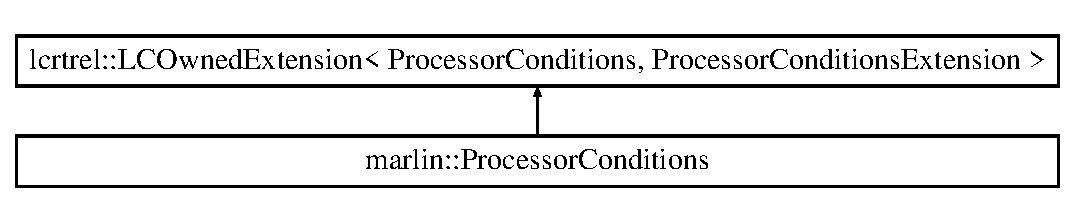
\includegraphics[height=2.000000cm]{structmarlin_1_1ProcessorConditions}
\end{center}
\end{figure}


The documentation for this struct was generated from the following file\+:\begin{DoxyCompactItemize}
\item 
Event\+Extensions.\+h\end{DoxyCompactItemize}

\section{marlin\+:\+:Processor\+Conditions\+Extension Class Reference}
\label{classmarlin_1_1ProcessorConditionsExtension}\index{marlin\+::\+Processor\+Conditions\+Extension@{marlin\+::\+Processor\+Conditions\+Extension}}


\doxyref{Processor\+Conditions\+Extension}{p.}{classmarlin_1_1ProcessorConditionsExtension} class Event extension providing access to processor runtime conditions (\doxyref{Logical\+Expressions}{p.}{classmarlin_1_1LogicalExpressions})  




{\ttfamily \#include $<$Event\+Extensions.\+h$>$}

\subsection*{Public Types}
\begin{DoxyCompactItemize}
\item 
\mbox{\label{classmarlin_1_1ProcessorConditionsExtension_a4b1d9cd86a28639264b1eb1ab877dae8}} 
using {\bfseries Conditions} = std\+::shared\+\_\+ptr$<$ \textbf{ Logical\+Expressions} $>$
\item 
\mbox{\label{classmarlin_1_1ProcessorConditionsExtension_a2745b1c85121c004694423d1253c225c}} 
using {\bfseries Conditions\+Map} = std\+::map$<$ std\+::string, std\+::string $>$
\end{DoxyCompactItemize}
\subsection*{Public Member Functions}
\begin{DoxyCompactItemize}
\item 
\mbox{\label{classmarlin_1_1ProcessorConditionsExtension_a0a4cb36b7879852960a8325fdd1ecf91}} 
{\bfseries Processor\+Conditions\+Extension} (const \textbf{ Processor\+Conditions\+Extension} \&)=delete
\item 
\mbox{\label{classmarlin_1_1ProcessorConditionsExtension_a358177e2724aacf9b187da9c4fdebaf1}} 
\textbf{ Processor\+Conditions\+Extension} \& {\bfseries operator=} (const \textbf{ Processor\+Conditions\+Extension} \&)=delete
\item 
\textbf{ Processor\+Conditions\+Extension} (const Conditions\+Map \&conds)
\begin{DoxyCompactList}\small\item\em Constructor. \end{DoxyCompactList}\item 
void \textbf{ set} (const \textbf{ Processor} $\ast$const processor, bool value)
\begin{DoxyCompactList}\small\item\em Set the runtime condition of the processor. \end{DoxyCompactList}\item 
void \textbf{ set} (const \textbf{ Processor} $\ast$const processor, const std\+::string \&name, bool value)
\begin{DoxyCompactList}\small\item\em Set the named runtime condition of the processor. \end{DoxyCompactList}\item 
bool \textbf{ check} (const std\+::string \&name) const
\begin{DoxyCompactList}\small\item\em Check whether the runtime condition is true. \end{DoxyCompactList}\end{DoxyCompactItemize}


\subsection{Detailed Description}
\doxyref{Processor\+Conditions\+Extension}{p.}{classmarlin_1_1ProcessorConditionsExtension} class Event extension providing access to processor runtime conditions (\doxyref{Logical\+Expressions}{p.}{classmarlin_1_1LogicalExpressions}) 

\subsection{Constructor \& Destructor Documentation}
\mbox{\label{classmarlin_1_1ProcessorConditionsExtension_a1a1c237bc18d2ff0c8021ae81eeeef1e}} 
\index{marlin\+::\+Processor\+Conditions\+Extension@{marlin\+::\+Processor\+Conditions\+Extension}!Processor\+Conditions\+Extension@{Processor\+Conditions\+Extension}}
\index{Processor\+Conditions\+Extension@{Processor\+Conditions\+Extension}!marlin\+::\+Processor\+Conditions\+Extension@{marlin\+::\+Processor\+Conditions\+Extension}}
\subsubsection{Processor\+Conditions\+Extension()}
{\footnotesize\ttfamily marlin\+::\+Processor\+Conditions\+Extension\+::\+Processor\+Conditions\+Extension (\begin{DoxyParamCaption}\item[{const Conditions\+Map \&}]{conds }\end{DoxyParamCaption})}



Constructor. 


\begin{DoxyParams}{Parameters}
{\em conds} & the initial runtime condition of the event (from steering file) \\
\hline
\end{DoxyParams}


\subsection{Member Function Documentation}
\mbox{\label{classmarlin_1_1ProcessorConditionsExtension_a48893f1f1157c70087574b83cb0f3e24}} 
\index{marlin\+::\+Processor\+Conditions\+Extension@{marlin\+::\+Processor\+Conditions\+Extension}!check@{check}}
\index{check@{check}!marlin\+::\+Processor\+Conditions\+Extension@{marlin\+::\+Processor\+Conditions\+Extension}}
\subsubsection{check()}
{\footnotesize\ttfamily bool marlin\+::\+Processor\+Conditions\+Extension\+::check (\begin{DoxyParamCaption}\item[{const std\+::string \&}]{name }\end{DoxyParamCaption}) const}



Check whether the runtime condition is true. 


\begin{DoxyParams}{Parameters}
{\em name} & the condition name \\
\hline
\end{DoxyParams}
\mbox{\label{classmarlin_1_1ProcessorConditionsExtension_ab4d96491ec3f605938a66ef55839c83f}} 
\index{marlin\+::\+Processor\+Conditions\+Extension@{marlin\+::\+Processor\+Conditions\+Extension}!set@{set}}
\index{set@{set}!marlin\+::\+Processor\+Conditions\+Extension@{marlin\+::\+Processor\+Conditions\+Extension}}
\subsubsection{set()\hspace{0.1cm}{\footnotesize\ttfamily [1/2]}}
{\footnotesize\ttfamily void marlin\+::\+Processor\+Conditions\+Extension\+::set (\begin{DoxyParamCaption}\item[{const \textbf{ Processor} $\ast$const}]{processor,  }\item[{bool}]{value }\end{DoxyParamCaption})}



Set the runtime condition of the processor. 


\begin{DoxyParams}{Parameters}
{\em processor} & the processor pointer \\
\hline
{\em value} & the runtime condition to set \\
\hline
\end{DoxyParams}


References marlin\+::\+Processor\+::name().

\mbox{\label{classmarlin_1_1ProcessorConditionsExtension_aa649c129dd572fca8f297f79b2cb8945}} 
\index{marlin\+::\+Processor\+Conditions\+Extension@{marlin\+::\+Processor\+Conditions\+Extension}!set@{set}}
\index{set@{set}!marlin\+::\+Processor\+Conditions\+Extension@{marlin\+::\+Processor\+Conditions\+Extension}}
\subsubsection{set()\hspace{0.1cm}{\footnotesize\ttfamily [2/2]}}
{\footnotesize\ttfamily void marlin\+::\+Processor\+Conditions\+Extension\+::set (\begin{DoxyParamCaption}\item[{const \textbf{ Processor} $\ast$const}]{processor,  }\item[{const std\+::string \&}]{name,  }\item[{bool}]{value }\end{DoxyParamCaption})}



Set the named runtime condition of the processor. 


\begin{DoxyParams}{Parameters}
{\em processor} & the processor pointer \\
\hline
{\em name} & the condition name \\
\hline
{\em value} & the runtime condition to set \\
\hline
\end{DoxyParams}


References marlin\+::\+Processor\+::name().



The documentation for this class was generated from the following files\+:\begin{DoxyCompactItemize}
\item 
Event\+Extensions.\+h\item 
Event\+Extensions.\+cc\end{DoxyCompactItemize}

\section{marlin\+:\+:concurrency\+:\+:Processor\+Sequence\+Worker Class Reference}
\label{classmarlin_1_1concurrency_1_1ProcessorSequenceWorker}\index{marlin\+::concurrency\+::\+Processor\+Sequence\+Worker@{marlin\+::concurrency\+::\+Processor\+Sequence\+Worker}}


\doxyref{Processor\+Sequence\+Worker}{p.}{classmarlin_1_1concurrency_1_1ProcessorSequenceWorker} class.  


Inheritance diagram for marlin\+:\+:concurrency\+:\+:Processor\+Sequence\+Worker\+:\begin{figure}[H]
\begin{center}
\leavevmode
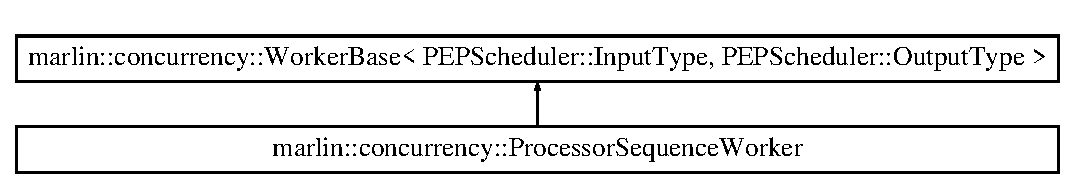
\includegraphics[height=2.000000cm]{classmarlin_1_1concurrency_1_1ProcessorSequenceWorker}
\end{center}
\end{figure}
\subsection*{Public Types}
\begin{DoxyCompactItemize}
\item 
\mbox{\label{classmarlin_1_1concurrency_1_1ProcessorSequenceWorker_a7207c7ed596a448c983b6238f0ea132d}} 
using {\bfseries Base} = \textbf{ Worker\+Base}$<$ P\+E\+P\+Scheduler\+::\+Input\+Type, \textbf{ P\+E\+P\+Scheduler\+::\+Output\+Type} $>$
\item 
\mbox{\label{classmarlin_1_1concurrency_1_1ProcessorSequenceWorker_a06ee28b1893db199ef150cb0c54db7a3}} 
using {\bfseries Input} = Base\+::\+Input
\item 
\mbox{\label{classmarlin_1_1concurrency_1_1ProcessorSequenceWorker_a31a0086b22d6ee468656fae6fbcf024c}} 
using {\bfseries Output} = Base\+::\+Output
\end{DoxyCompactItemize}
\subsection*{Public Member Functions}
\begin{DoxyCompactItemize}
\item 
\textbf{ Processor\+Sequence\+Worker} (std\+::shared\+\_\+ptr$<$ \textbf{ Sequence} $>$ sequence)
\begin{DoxyCompactList}\small\item\em Constructor. \end{DoxyCompactList}\end{DoxyCompactItemize}
\subsection*{Additional Inherited Members}


\subsection{Detailed Description}
\doxyref{Processor\+Sequence\+Worker}{p.}{classmarlin_1_1concurrency_1_1ProcessorSequenceWorker} class. 

\subsection{Constructor \& Destructor Documentation}
\mbox{\label{classmarlin_1_1concurrency_1_1ProcessorSequenceWorker_a901aa05b53666ec3bdf92384fdd935ea}} 
\index{marlin\+::concurrency\+::\+Processor\+Sequence\+Worker@{marlin\+::concurrency\+::\+Processor\+Sequence\+Worker}!Processor\+Sequence\+Worker@{Processor\+Sequence\+Worker}}
\index{Processor\+Sequence\+Worker@{Processor\+Sequence\+Worker}!marlin\+::concurrency\+::\+Processor\+Sequence\+Worker@{marlin\+::concurrency\+::\+Processor\+Sequence\+Worker}}
\subsubsection{Processor\+Sequence\+Worker()}
{\footnotesize\ttfamily marlin\+::concurrency\+::\+Processor\+Sequence\+Worker\+::\+Processor\+Sequence\+Worker (\begin{DoxyParamCaption}\item[{std\+::shared\+\_\+ptr$<$ \textbf{ Sequence} $>$}]{sequence }\end{DoxyParamCaption})}



Constructor. 


\begin{DoxyParams}{Parameters}
{\em sequence} & the processor sequence to execute \\
\hline
\end{DoxyParams}


The documentation for this class was generated from the following file\+:\begin{DoxyCompactItemize}
\item 
P\+E\+P\+Scheduler.\+cc\end{DoxyCompactItemize}

\section{marlin\+:\+:concurrency\+:\+:Queue$<$ T, class $>$ Class Template Reference}
\label{classmarlin_1_1concurrency_1_1Queue}\index{marlin\+::concurrency\+::\+Queue$<$ T, class $>$@{marlin\+::concurrency\+::\+Queue$<$ T, class $>$}}


\doxyref{Queue}{p.}{classmarlin_1_1concurrency_1_1Queue} class.  




{\ttfamily \#include $<$Queue.\+h$>$}

\subsection*{Public Member Functions}
\begin{DoxyCompactItemize}
\item 
\mbox{\label{classmarlin_1_1concurrency_1_1Queue_a53dd670d5a3928b5a7f7a0513dfabc0a}} 
{\bfseries Queue} (const \textbf{ Queue} \&)=delete
\item 
\mbox{\label{classmarlin_1_1concurrency_1_1Queue_a8e883c52c4c280ac39b1481e67bd2c4d}} 
\textbf{ Queue} \& {\bfseries operator=} (const \textbf{ Queue} \&)=delete
\item 
\textbf{ Queue} (std\+::size\+\_\+t maxsize)
\begin{DoxyCompactList}\small\item\em Constructor. \end{DoxyCompactList}\item 
bool \textbf{ push} (T \&value)
\begin{DoxyCompactList}\small\item\em Push a value to the queue. \end{DoxyCompactList}\item 
bool \textbf{ pop} (T \&value)
\begin{DoxyCompactList}\small\item\em Pop and get the front element in the queue. \end{DoxyCompactList}\item 
\mbox{\label{classmarlin_1_1concurrency_1_1Queue_a497bb57e19681a081a1ee39f586525c0}} 
bool \textbf{ empty} () const
\begin{DoxyCompactList}\small\item\em Whether the queue is empty. \end{DoxyCompactList}\item 
\mbox{\label{classmarlin_1_1concurrency_1_1Queue_a11cbf80dbde64a3e1de97e31ba33b7e2}} 
std\+::size\+\_\+t \textbf{ max\+Size} () const
\begin{DoxyCompactList}\small\item\em Get the maximum queue size. \end{DoxyCompactList}\item 
std\+::size\+\_\+t \textbf{ set\+Max\+Size} (std\+::size\+\_\+t maxsize)
\begin{DoxyCompactList}\small\item\em Set the maximum queue size. \end{DoxyCompactList}\item 
\mbox{\label{classmarlin_1_1concurrency_1_1Queue_a388205ed7f30569b1f905b038f329913}} 
bool \textbf{ is\+Full} () const
\begin{DoxyCompactList}\small\item\em Check whether the queue has reached the maximum allowed size. \end{DoxyCompactList}\item 
\mbox{\label{classmarlin_1_1concurrency_1_1Queue_a8837ff5f16351afd14b7944aa2716b8c}} 
void \textbf{ clear} ()
\begin{DoxyCompactList}\small\item\em Clear the queue. \end{DoxyCompactList}\item 
\mbox{\label{classmarlin_1_1concurrency_1_1Queue_a6b0cc8fcd822ca7a2800d4dfb3076b3b}} 
std\+::size\+\_\+t \textbf{ free\+Slots} () const
\begin{DoxyCompactList}\small\item\em Get the number of free slots in the queue. \end{DoxyCompactList}\end{DoxyCompactItemize}


\subsection{Detailed Description}
\subsubsection*{template$<$typename T, class = typename std\+::enable\+\_\+if$<$std\+::is\+\_\+move\+\_\+assignable$<$\+T$>$\+::value$>$\+::type$>$\newline
class marlin\+::concurrency\+::\+Queue$<$ T, class $>$}

\doxyref{Queue}{p.}{classmarlin_1_1concurrency_1_1Queue} class. 

A simplified thread safe queue container. Support maximum size setting. The type T must implement move assignement 

\subsection{Constructor \& Destructor Documentation}
\mbox{\label{classmarlin_1_1concurrency_1_1Queue_afe1d46cf1cabafc9ad60da7df3905a5f}} 
\index{marlin\+::concurrency\+::\+Queue@{marlin\+::concurrency\+::\+Queue}!Queue@{Queue}}
\index{Queue@{Queue}!marlin\+::concurrency\+::\+Queue@{marlin\+::concurrency\+::\+Queue}}
\subsubsection{Queue()}
{\footnotesize\ttfamily template$<$typename T, class  = typename std\+::enable\+\_\+if$<$std\+::is\+\_\+move\+\_\+assignable$<$\+T$>$\+::value$>$\+::type$>$ \\
\textbf{ marlin\+::concurrency\+::\+Queue}$<$ T, class $>$\+::\textbf{ Queue} (\begin{DoxyParamCaption}\item[{std\+::size\+\_\+t}]{maxsize }\end{DoxyParamCaption})\hspace{0.3cm}{\ttfamily [inline]}}



Constructor. 


\begin{DoxyParams}{Parameters}
{\em maxsize} & the maximum queue size \\
\hline
\end{DoxyParams}


\subsection{Member Function Documentation}
\mbox{\label{classmarlin_1_1concurrency_1_1Queue_a2a4fe2f64d546fca839ed30121cc2052}} 
\index{marlin\+::concurrency\+::\+Queue@{marlin\+::concurrency\+::\+Queue}!pop@{pop}}
\index{pop@{pop}!marlin\+::concurrency\+::\+Queue@{marlin\+::concurrency\+::\+Queue}}
\subsubsection{pop()}
{\footnotesize\ttfamily template$<$typename T, class  = typename std\+::enable\+\_\+if$<$std\+::is\+\_\+move\+\_\+assignable$<$\+T$>$\+::value$>$\+::type$>$ \\
bool \textbf{ marlin\+::concurrency\+::\+Queue}$<$ T, class $>$\+::pop (\begin{DoxyParamCaption}\item[{T \&}]{value }\end{DoxyParamCaption})\hspace{0.3cm}{\ttfamily [inline]}}



Pop and get the front element in the queue. 

The queue type must support move operation


\begin{DoxyParams}{Parameters}
{\em value} & the value to receive \\
\hline
\end{DoxyParams}


Referenced by marlin\+::concurrency\+::\+Worker$<$ I\+N, O\+U\+T $>$\+::run().

\mbox{\label{classmarlin_1_1concurrency_1_1Queue_ae94c11f312c643b8737a1827f7aa2a80}} 
\index{marlin\+::concurrency\+::\+Queue@{marlin\+::concurrency\+::\+Queue}!push@{push}}
\index{push@{push}!marlin\+::concurrency\+::\+Queue@{marlin\+::concurrency\+::\+Queue}}
\subsubsection{push()}
{\footnotesize\ttfamily template$<$typename T, class  = typename std\+::enable\+\_\+if$<$std\+::is\+\_\+move\+\_\+assignable$<$\+T$>$\+::value$>$\+::type$>$ \\
bool \textbf{ marlin\+::concurrency\+::\+Queue}$<$ T, class $>$\+::push (\begin{DoxyParamCaption}\item[{T \&}]{value }\end{DoxyParamCaption})\hspace{0.3cm}{\ttfamily [inline]}}



Push a value to the queue. 

W\+A\+R\+N\+I\+NG\+: On success, the element is moved in the queue container, else it is not !


\begin{DoxyParams}{Parameters}
{\em value} & the value to push \\
\hline
\end{DoxyParams}
\mbox{\label{classmarlin_1_1concurrency_1_1Queue_a5ab6fbc8d0df4c9e9e7925692141c563}} 
\index{marlin\+::concurrency\+::\+Queue@{marlin\+::concurrency\+::\+Queue}!set\+Max\+Size@{set\+Max\+Size}}
\index{set\+Max\+Size@{set\+Max\+Size}!marlin\+::concurrency\+::\+Queue@{marlin\+::concurrency\+::\+Queue}}
\subsubsection{set\+Max\+Size()}
{\footnotesize\ttfamily template$<$typename T, class  = typename std\+::enable\+\_\+if$<$std\+::is\+\_\+move\+\_\+assignable$<$\+T$>$\+::value$>$\+::type$>$ \\
std\+::size\+\_\+t \textbf{ marlin\+::concurrency\+::\+Queue}$<$ T, class $>$\+::set\+Max\+Size (\begin{DoxyParamCaption}\item[{std\+::size\+\_\+t}]{maxsize }\end{DoxyParamCaption})\hspace{0.3cm}{\ttfamily [inline]}}



Set the maximum queue size. 

Note that the queue is N\+OT resized if the new value is smaller than the old size. The value of the old max size is returned


\begin{DoxyParams}{Parameters}
{\em maxsize} & the maximum queue size to set \\
\hline
\end{DoxyParams}


The documentation for this class was generated from the following file\+:\begin{DoxyCompactItemize}
\item 
Queue.\+h\end{DoxyCompactItemize}

\section{marlin\+:\+:concurrency\+:\+:Queue\+Element$<$ IN, O\+UT $>$ Class Template Reference}
\label{classmarlin_1_1concurrency_1_1QueueElement}\index{marlin\+::concurrency\+::\+Queue\+Element$<$ I\+N, O\+U\+T $>$@{marlin\+::concurrency\+::\+Queue\+Element$<$ I\+N, O\+U\+T $>$}}


\doxyref{Queue\+Element}{p.}{classmarlin_1_1concurrency_1_1QueueElement} class A template queue element used in the thread pool.  




{\ttfamily \#include $<$Queue\+Element.\+h$>$}

\subsection*{Public Member Functions}
\begin{DoxyCompactItemize}
\item 
\mbox{\label{classmarlin_1_1concurrency_1_1QueueElement_a462951784529390d2adb452d0e2a7f95}} 
{\bfseries Queue\+Element} (const \textbf{ Queue\+Element}$<$ IN, O\+UT $>$ \&)=delete
\item 
\mbox{\label{classmarlin_1_1concurrency_1_1QueueElement_a0dce6fcc5d388214b031d146986cfba7}} 
\textbf{ Queue\+Element} \& {\bfseries operator=} (const \textbf{ Queue\+Element}$<$ IN, O\+UT $>$ \&)=delete
\item 
\textbf{ Queue\+Element} (IN \&\&input)
\begin{DoxyCompactList}\small\item\em Constructor with input data. \end{DoxyCompactList}\item 
\mbox{\label{classmarlin_1_1concurrency_1_1QueueElement_a8d17ddda4ecda3206b1cbbf025682eb1}} 
\textbf{ Queue\+Element} (\textbf{ Queue\+Element}$<$ IN, O\+UT $>$ \&\&rhs)
\begin{DoxyCompactList}\small\item\em Move constructor. \end{DoxyCompactList}\item 
\mbox{\label{classmarlin_1_1concurrency_1_1QueueElement_afe197a16c9be7da5814cfa77b934b2fc}} 
\textbf{ Queue\+Element} \& \textbf{ operator=} (\textbf{ Queue\+Element}$<$ IN, O\+UT $>$ \&\&rhs)
\begin{DoxyCompactList}\small\item\em Move assignement operator. \end{DoxyCompactList}\item 
\mbox{\label{classmarlin_1_1concurrency_1_1QueueElement_a2a0d44a899a808ae03579c166be896c6}} 
std\+::shared\+\_\+ptr$<$ std\+::promise$<$ O\+UT $>$ $>$ \textbf{ promise} () const
\begin{DoxyCompactList}\small\item\em Get the output promise. \end{DoxyCompactList}\item 
void \textbf{ set\+Value} (O\+UT \&\&output)
\begin{DoxyCompactList}\small\item\em Set the value to be retrieved in the future variable. \end{DoxyCompactList}\item 
IN \textbf{ take\+Input} ()
\begin{DoxyCompactList}\small\item\em Take the input data. \end{DoxyCompactList}\end{DoxyCompactItemize}


\subsection{Detailed Description}
\subsubsection*{template$<$typename IN, typename O\+UT$>$\newline
class marlin\+::concurrency\+::\+Queue\+Element$<$ I\+N, O\+U\+T $>$}

\doxyref{Queue\+Element}{p.}{classmarlin_1_1concurrency_1_1QueueElement} class A template queue element used in the thread pool. 

The IN type represent the actual data type pushed by the user in the thread pool queue and the O\+UT type the expected output stored in the future object returned by calling push() 

\subsection{Constructor \& Destructor Documentation}
\mbox{\label{classmarlin_1_1concurrency_1_1QueueElement_a45a6848fdd4728381231e43437c92d8f}} 
\index{marlin\+::concurrency\+::\+Queue\+Element@{marlin\+::concurrency\+::\+Queue\+Element}!Queue\+Element@{Queue\+Element}}
\index{Queue\+Element@{Queue\+Element}!marlin\+::concurrency\+::\+Queue\+Element@{marlin\+::concurrency\+::\+Queue\+Element}}
\subsubsection{Queue\+Element()}
{\footnotesize\ttfamily template$<$typename IN, typename O\+UT$>$ \\
\textbf{ marlin\+::concurrency\+::\+Queue\+Element}$<$ IN, O\+UT $>$\+::\textbf{ Queue\+Element} (\begin{DoxyParamCaption}\item[{IN \&\&}]{input }\end{DoxyParamCaption})\hspace{0.3cm}{\ttfamily [inline]}}



Constructor with input data. 


\begin{DoxyParams}{Parameters}
{\em input} & user input data \\
\hline
\end{DoxyParams}


\subsection{Member Function Documentation}
\mbox{\label{classmarlin_1_1concurrency_1_1QueueElement_a1df07f4a80f4764a9cec499e861dcf66}} 
\index{marlin\+::concurrency\+::\+Queue\+Element@{marlin\+::concurrency\+::\+Queue\+Element}!set\+Value@{set\+Value}}
\index{set\+Value@{set\+Value}!marlin\+::concurrency\+::\+Queue\+Element@{marlin\+::concurrency\+::\+Queue\+Element}}
\subsubsection{set\+Value()}
{\footnotesize\ttfamily template$<$typename IN, typename O\+UT$>$ \\
void \textbf{ marlin\+::concurrency\+::\+Queue\+Element}$<$ IN, O\+UT $>$\+::set\+Value (\begin{DoxyParamCaption}\item[{O\+UT \&\&}]{output }\end{DoxyParamCaption})\hspace{0.3cm}{\ttfamily [inline]}}



Set the value to be retrieved in the future variable. 


\begin{DoxyParams}{Parameters}
{\em output} & the output data to retrieve in the future object \\
\hline
\end{DoxyParams}


Referenced by marlin\+::concurrency\+::\+Worker\+Base$<$ P\+E\+P\+Scheduler\+::\+Input\+Type, P\+E\+P\+Scheduler\+::\+Output\+Type $>$\+::process\+Element().

\mbox{\label{classmarlin_1_1concurrency_1_1QueueElement_a1a04765bc6f3bfa7fefef55f76693c62}} 
\index{marlin\+::concurrency\+::\+Queue\+Element@{marlin\+::concurrency\+::\+Queue\+Element}!take\+Input@{take\+Input}}
\index{take\+Input@{take\+Input}!marlin\+::concurrency\+::\+Queue\+Element@{marlin\+::concurrency\+::\+Queue\+Element}}
\subsubsection{take\+Input()}
{\footnotesize\ttfamily template$<$typename IN, typename O\+UT$>$ \\
IN \textbf{ marlin\+::concurrency\+::\+Queue\+Element}$<$ IN, O\+UT $>$\+::take\+Input (\begin{DoxyParamCaption}{ }\end{DoxyParamCaption})\hspace{0.3cm}{\ttfamily [inline]}}



Take the input data. 

Note that this moves the input data and thus invalidate the stored input data of the queue element 

Referenced by marlin\+::concurrency\+::\+Worker\+Base$<$ P\+E\+P\+Scheduler\+::\+Input\+Type, P\+E\+P\+Scheduler\+::\+Output\+Type $>$\+::process\+Element().



The documentation for this class was generated from the following file\+:\begin{DoxyCompactItemize}
\item 
Queue\+Element.\+h\end{DoxyCompactItemize}

\section{marlin\+:\+:concurrency\+:\+:Queue\+Element$<$ IN, void $>$ Class Template Reference}
\label{classmarlin_1_1concurrency_1_1QueueElement_3_01IN_00_01void_01_4}\index{marlin\+::concurrency\+::\+Queue\+Element$<$ I\+N, void $>$@{marlin\+::concurrency\+::\+Queue\+Element$<$ I\+N, void $>$}}
\subsection*{Public Member Functions}
\begin{DoxyCompactItemize}
\item 
\mbox{\label{classmarlin_1_1concurrency_1_1QueueElement_3_01IN_00_01void_01_4_a08306fa5693a03daa8e4c938b549a2ba}} 
{\bfseries Queue\+Element} (const \textbf{ Queue\+Element}$<$ IN, void $>$ \&)=delete
\item 
\mbox{\label{classmarlin_1_1concurrency_1_1QueueElement_3_01IN_00_01void_01_4_ab0843a8fba82c927967594161c29fa53}} 
\textbf{ Queue\+Element} \& {\bfseries operator=} (const \textbf{ Queue\+Element}$<$ IN, void $>$ \&)=delete
\item 
\mbox{\label{classmarlin_1_1concurrency_1_1QueueElement_3_01IN_00_01void_01_4_ad62984e1aecd6f588d711215664820be}} 
{\bfseries Queue\+Element} (IN \&\&input)
\item 
\mbox{\label{classmarlin_1_1concurrency_1_1QueueElement_3_01IN_00_01void_01_4_a61456d2ff3b330edfd54fbe08f6cd281}} 
{\bfseries Queue\+Element} (\textbf{ Queue\+Element}$<$ IN, void $>$ \&\&rhs)
\item 
\mbox{\label{classmarlin_1_1concurrency_1_1QueueElement_3_01IN_00_01void_01_4_adacf41504baeedcf8874703ee2e89f96}} 
\textbf{ Queue\+Element} \& {\bfseries operator=} (\textbf{ Queue\+Element}$<$ IN, void $>$ \&\&rhs)
\item 
\mbox{\label{classmarlin_1_1concurrency_1_1QueueElement_3_01IN_00_01void_01_4_a88c480ef48ce66a2acf186fd379993cf}} 
std\+::shared\+\_\+ptr$<$ std\+::promise$<$ void $>$ $>$ {\bfseries promise} () const
\item 
\mbox{\label{classmarlin_1_1concurrency_1_1QueueElement_3_01IN_00_01void_01_4_a9d3f230b22cee255053094125c3baaa3}} 
void {\bfseries set\+Value} ()
\item 
\mbox{\label{classmarlin_1_1concurrency_1_1QueueElement_3_01IN_00_01void_01_4_a7e2a3ada89d3819c75271fa62778491d}} 
IN {\bfseries take\+Input} ()
\end{DoxyCompactItemize}


The documentation for this class was generated from the following file\+:\begin{DoxyCompactItemize}
\item 
Queue\+Element.\+h\end{DoxyCompactItemize}

\section{marlin\+:\+:concurrency\+:\+:Queue\+Element$<$ void, O\+UT $>$ Class Template Reference}
\label{classmarlin_1_1concurrency_1_1QueueElement_3_01void_00_01OUT_01_4}\index{marlin\+::concurrency\+::\+Queue\+Element$<$ void, O\+U\+T $>$@{marlin\+::concurrency\+::\+Queue\+Element$<$ void, O\+U\+T $>$}}
\subsection*{Public Member Functions}
\begin{DoxyCompactItemize}
\item 
\mbox{\label{classmarlin_1_1concurrency_1_1QueueElement_3_01void_00_01OUT_01_4_a52c04239dfdacc7c509c64d48eb2773c}} 
{\bfseries Queue\+Element} (const \textbf{ Queue\+Element}$<$ void, O\+UT $>$ \&)=delete
\item 
\mbox{\label{classmarlin_1_1concurrency_1_1QueueElement_3_01void_00_01OUT_01_4_a71fce0a691591530079c2e5e1f42753c}} 
\textbf{ Queue\+Element} \& {\bfseries operator=} (const \textbf{ Queue\+Element}$<$ void, O\+UT $>$ \&)=delete
\item 
\mbox{\label{classmarlin_1_1concurrency_1_1QueueElement_3_01void_00_01OUT_01_4_ac535c4942de170b11a4602b2d2b9309b}} 
{\bfseries Queue\+Element} (\textbf{ Queue\+Element}$<$ void, O\+UT $>$ \&\&rhs)
\item 
\mbox{\label{classmarlin_1_1concurrency_1_1QueueElement_3_01void_00_01OUT_01_4_a2ec881dc373eeac9a4ccde492e22f69b}} 
\textbf{ Queue\+Element} \& {\bfseries operator=} (\textbf{ Queue\+Element}$<$ void, O\+UT $>$ \&\&rhs)
\item 
\mbox{\label{classmarlin_1_1concurrency_1_1QueueElement_3_01void_00_01OUT_01_4_a4c5c741751dc184988651524fc704849}} 
std\+::shared\+\_\+ptr$<$ std\+::promise$<$ O\+UT $>$ $>$ {\bfseries promise} () const
\item 
\mbox{\label{classmarlin_1_1concurrency_1_1QueueElement_3_01void_00_01OUT_01_4_afe0bed3f8e980b9124a81e9edafbd6f0}} 
void {\bfseries set\+Value} (O\+UT \&\&output)
\end{DoxyCompactItemize}


The documentation for this class was generated from the following file\+:\begin{DoxyCompactItemize}
\item 
Queue\+Element.\+h\end{DoxyCompactItemize}

\section{marlin\+:\+:concurrency\+:\+:Queue\+Element$<$ void, void $>$ Class Template Reference}
\label{classmarlin_1_1concurrency_1_1QueueElement_3_01void_00_01void_01_4}\index{marlin\+::concurrency\+::\+Queue\+Element$<$ void, void $>$@{marlin\+::concurrency\+::\+Queue\+Element$<$ void, void $>$}}
\subsection*{Public Member Functions}
\begin{DoxyCompactItemize}
\item 
\mbox{\label{classmarlin_1_1concurrency_1_1QueueElement_3_01void_00_01void_01_4_a7963e94cd147b135f16af4d5f624096f}} 
{\bfseries Queue\+Element} (const \textbf{ Queue\+Element}$<$ void, void $>$ \&)=delete
\item 
\mbox{\label{classmarlin_1_1concurrency_1_1QueueElement_3_01void_00_01void_01_4_afbeb47bfd74d5d55e93de053729c56cd}} 
\textbf{ Queue\+Element} \& {\bfseries operator=} (const \textbf{ Queue\+Element}$<$ void, void $>$ \&)=delete
\item 
\mbox{\label{classmarlin_1_1concurrency_1_1QueueElement_3_01void_00_01void_01_4_a056f749849a2f82e77d8913e44711557}} 
{\bfseries Queue\+Element} (\textbf{ Queue\+Element}$<$ void, void $>$ \&\&rhs)
\item 
\mbox{\label{classmarlin_1_1concurrency_1_1QueueElement_3_01void_00_01void_01_4_aef94dac7ba236b1a8cd3e678255893d8}} 
\textbf{ Queue\+Element} \& {\bfseries operator=} (\textbf{ Queue\+Element}$<$ void, void $>$ \&\&rhs)
\item 
\mbox{\label{classmarlin_1_1concurrency_1_1QueueElement_3_01void_00_01void_01_4_a3c6c05b1de010e22e7b2097835960175}} 
std\+::shared\+\_\+ptr$<$ std\+::promise$<$ void $>$ $>$ {\bfseries promise} () const
\item 
\mbox{\label{classmarlin_1_1concurrency_1_1QueueElement_3_01void_00_01void_01_4_aede68df98bf8e4761f326c02321c65c2}} 
void {\bfseries set\+Value} ()
\end{DoxyCompactItemize}


The documentation for this class was generated from the following file\+:\begin{DoxyCompactItemize}
\item 
Queue\+Element.\+h\end{DoxyCompactItemize}

\section{marlin\+:\+:Random\+Seed Struct Reference}
\label{structmarlin_1_1RandomSeed}\index{marlin\+::\+Random\+Seed@{marlin\+::\+Random\+Seed}}
Inheritance diagram for marlin\+:\+:Random\+Seed\+:\begin{figure}[H]
\begin{center}
\leavevmode
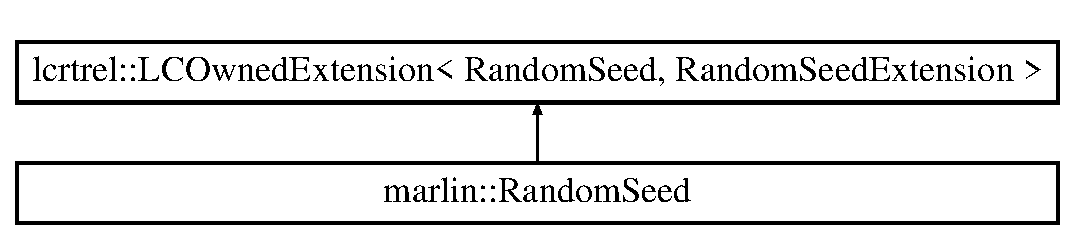
\includegraphics[height=2.000000cm]{structmarlin_1_1RandomSeed}
\end{center}
\end{figure}


The documentation for this struct was generated from the following file\+:\begin{DoxyCompactItemize}
\item 
Event\+Extensions.\+h\end{DoxyCompactItemize}

\section{marlin\+:\+:Random\+Seed\+Extension Class Reference}
\label{classmarlin_1_1RandomSeedExtension}\index{marlin\+::\+Random\+Seed\+Extension@{marlin\+::\+Random\+Seed\+Extension}}


\doxyref{Random\+Seed\+Extension}{p.}{classmarlin_1_1RandomSeedExtension} class Event extension providing access to random seeds.  




{\ttfamily \#include $<$Event\+Extensions.\+h$>$}

\subsection*{Public Types}
\begin{DoxyCompactItemize}
\item 
\mbox{\label{classmarlin_1_1RandomSeedExtension_a988c9b4f409f8a756f78f325f53b2788}} 
using {\bfseries Random\+Seed\+Map} = std\+::unique\+\_\+ptr$<$ Random\+Seed\+Manager\+::\+Random\+Seed\+Map $>$
\item 
\mbox{\label{classmarlin_1_1RandomSeedExtension_af2c49ce62d77583439c41bf305e1ce14}} 
using {\bfseries Random\+Seed\+Type} = Random\+Seed\+Manager\+::\+Seed\+Type
\end{DoxyCompactItemize}
\subsection*{Public Member Functions}
\begin{DoxyCompactItemize}
\item 
\mbox{\label{classmarlin_1_1RandomSeedExtension_a230b61a07f10a420346076564dce4917}} 
{\bfseries Random\+Seed\+Extension} (const \textbf{ Random\+Seed\+Extension} \&)=delete
\item 
\mbox{\label{classmarlin_1_1RandomSeedExtension_af7937e2bffdba6d3075b582c05db1896}} 
\textbf{ Random\+Seed\+Extension} \& {\bfseries operator=} (const \textbf{ Random\+Seed\+Extension} \&)=delete
\item 
\textbf{ Random\+Seed\+Extension} (Random\+Seed\+Map seeds)
\begin{DoxyCompactList}\small\item\em Constructor. \end{DoxyCompactList}\item 
Random\+Seed\+Type \textbf{ random\+Seed} (const \textbf{ Processor} $\ast$const processor) const
\begin{DoxyCompactList}\small\item\em Get the random seed for a given processor. \end{DoxyCompactList}\end{DoxyCompactItemize}


\subsection{Detailed Description}
\doxyref{Random\+Seed\+Extension}{p.}{classmarlin_1_1RandomSeedExtension} class Event extension providing access to random seeds. 

\subsection{Constructor \& Destructor Documentation}
\mbox{\label{classmarlin_1_1RandomSeedExtension_a712601308d021827076b36da7bb52e47}} 
\index{marlin\+::\+Random\+Seed\+Extension@{marlin\+::\+Random\+Seed\+Extension}!Random\+Seed\+Extension@{Random\+Seed\+Extension}}
\index{Random\+Seed\+Extension@{Random\+Seed\+Extension}!marlin\+::\+Random\+Seed\+Extension@{marlin\+::\+Random\+Seed\+Extension}}
\subsubsection{Random\+Seed\+Extension()}
{\footnotesize\ttfamily marlin\+::\+Random\+Seed\+Extension\+::\+Random\+Seed\+Extension (\begin{DoxyParamCaption}\item[{Random\+Seed\+Map}]{seeds }\end{DoxyParamCaption})}



Constructor. 


\begin{DoxyParams}{Parameters}
{\em seeds} & the random seed set for the current event \\
\hline
\end{DoxyParams}


\subsection{Member Function Documentation}
\mbox{\label{classmarlin_1_1RandomSeedExtension_a66d251314f49d07ddfef014894deccae}} 
\index{marlin\+::\+Random\+Seed\+Extension@{marlin\+::\+Random\+Seed\+Extension}!random\+Seed@{random\+Seed}}
\index{random\+Seed@{random\+Seed}!marlin\+::\+Random\+Seed\+Extension@{marlin\+::\+Random\+Seed\+Extension}}
\subsubsection{random\+Seed()}
{\footnotesize\ttfamily Random\+Seed\+Extension\+::\+Random\+Seed\+Type marlin\+::\+Random\+Seed\+Extension\+::random\+Seed (\begin{DoxyParamCaption}\item[{const \textbf{ Processor} $\ast$const}]{processor }\end{DoxyParamCaption}) const}



Get the random seed for a given processor. 


\begin{DoxyParams}{Parameters}
{\em processor} & the processor pointer \\
\hline
\end{DoxyParams}


References marlin\+::\+Processor\+::name().



The documentation for this class was generated from the following files\+:\begin{DoxyCompactItemize}
\item 
Event\+Extensions.\+h\item 
Event\+Extensions.\+cc\end{DoxyCompactItemize}

\section{marlin\+:\+:Random\+Seed\+Manager Class Reference}
\label{classmarlin_1_1RandomSeedManager}\index{marlin\+::\+Random\+Seed\+Manager@{marlin\+::\+Random\+Seed\+Manager}}


\doxyref{Random\+Seed\+Manager}{p.}{classmarlin_1_1RandomSeedManager} class.  




{\ttfamily \#include $<$Random\+Seed\+Manager.\+h$>$}

\subsection*{Public Types}
\begin{DoxyCompactItemize}
\item 
\mbox{\label{classmarlin_1_1RandomSeedManager_a22e7991f1e79ba1ac8770724dd99dfaf}} 
typedef unsigned int {\bfseries Seed\+Type}
\item 
\mbox{\label{classmarlin_1_1RandomSeedManager_a2b4db2a3645c39d14c3e8af615f6bc56}} 
typedef std\+::hash$<$ const void $\ast$ $>$ {\bfseries Hash\+Function}
\item 
\mbox{\label{classmarlin_1_1RandomSeedManager_a384ee1c8ab79d7a1c4f595300c063f2e}} 
typedef Hash\+Function\+::argument\+\_\+type {\bfseries Hash\+Argument}
\item 
\mbox{\label{classmarlin_1_1RandomSeedManager_a087cae390c126e1468d6354099740e3c}} 
typedef Hash\+Function\+::result\+\_\+type {\bfseries Hash\+Result}
\item 
\mbox{\label{classmarlin_1_1RandomSeedManager_a446223249f682903ceeaf59a9b3658dc}} 
typedef std\+::unordered\+\_\+set$<$ Hash\+Result $>$ {\bfseries Entry\+List}
\item 
\mbox{\label{classmarlin_1_1RandomSeedManager_a79a5b7b30c8e99560d736e7c1d14809c}} 
typedef std\+::map$<$ Hash\+Result, Seed\+Type $>$ {\bfseries Random\+Seed\+Map}
\item 
\mbox{\label{classmarlin_1_1RandomSeedManager_a7933b8c0d97b9848fec2dd85c44bb5f7}} 
typedef std\+::mt19937 {\bfseries Random\+Generator}
\item 
\mbox{\label{classmarlin_1_1RandomSeedManager_a6e4cebc8c94e68fb6ba72c2ec4b38e2d}} 
typedef std\+::uniform\+\_\+int\+\_\+distribution$<$ Seed\+Type $>$ {\bfseries Random\+Distribution}
\end{DoxyCompactItemize}
\subsection*{Public Member Functions}
\begin{DoxyCompactItemize}
\item 
\mbox{\label{classmarlin_1_1RandomSeedManager_ac6016749c5e09831cc882d7dc3f85b99}} 
{\bfseries Random\+Seed\+Manager} (const \textbf{ Random\+Seed\+Manager} \&)=delete
\item 
\mbox{\label{classmarlin_1_1RandomSeedManager_ae2324c7cc8f867a3dc4923f9ce1da452}} 
\textbf{ Random\+Seed\+Manager} \& {\bfseries operator=} (const \textbf{ Random\+Seed\+Manager} \&)=delete
\item 
\textbf{ Random\+Seed\+Manager} (Seed\+Type global\+Seed=time(nullptr))
\begin{DoxyCompactList}\small\item\em Constructor with global seed. \end{DoxyCompactList}\item 
void \textbf{ add\+Entry} (Hash\+Result entry)
\begin{DoxyCompactList}\small\item\em Add an entry to the random seed manager. \end{DoxyCompactList}\item 
void \textbf{ add\+Entry} (Hash\+Argument arg)
\begin{DoxyCompactList}\small\item\em Add an entry to the random seed manager. \end{DoxyCompactList}\item 
std\+::unique\+\_\+ptr$<$ Random\+Seed\+Map $>$ \textbf{ generate\+Random\+Seeds} (const E\+V\+E\+N\+T\+::\+L\+C\+Event $\ast$const evt)
\begin{DoxyCompactList}\small\item\em Generate a random seed map. \end{DoxyCompactList}\end{DoxyCompactItemize}
\subsection*{Static Public Attributes}
\begin{DoxyCompactItemize}
\item 
\mbox{\label{classmarlin_1_1RandomSeedManager_a3258392857a15bd92a4b9c204a0a9f52}} 
static const Seed\+Type {\bfseries Min\+Seed} = 0
\item 
\mbox{\label{classmarlin_1_1RandomSeedManager_a8b3c60f20510b92184477ebe8a599298}} 
static const Seed\+Type {\bfseries Max\+Seed} = std\+::numeric\+\_\+limits$<$Seed\+Type$>$\+::max()
\end{DoxyCompactItemize}


\subsection{Detailed Description}
\doxyref{Random\+Seed\+Manager}{p.}{classmarlin_1_1RandomSeedManager} class. 

\subsection{Constructor \& Destructor Documentation}
\mbox{\label{classmarlin_1_1RandomSeedManager_aff29e2ededf32a7e287d7808f1de2be2}} 
\index{marlin\+::\+Random\+Seed\+Manager@{marlin\+::\+Random\+Seed\+Manager}!Random\+Seed\+Manager@{Random\+Seed\+Manager}}
\index{Random\+Seed\+Manager@{Random\+Seed\+Manager}!marlin\+::\+Random\+Seed\+Manager@{marlin\+::\+Random\+Seed\+Manager}}
\subsubsection{Random\+Seed\+Manager()}
{\footnotesize\ttfamily marlin\+::\+Random\+Seed\+Manager\+::\+Random\+Seed\+Manager (\begin{DoxyParamCaption}\item[{Seed\+Type}]{global\+Seed = {\ttfamily time(nullptr)} }\end{DoxyParamCaption})}



Constructor with global seed. 


\begin{DoxyParams}{Parameters}
{\em global\+Seed} & the global seed \\
\hline
\end{DoxyParams}


\subsection{Member Function Documentation}
\mbox{\label{classmarlin_1_1RandomSeedManager_acae2cec3d0c02092b3632a1da6de75fa}} 
\index{marlin\+::\+Random\+Seed\+Manager@{marlin\+::\+Random\+Seed\+Manager}!add\+Entry@{add\+Entry}}
\index{add\+Entry@{add\+Entry}!marlin\+::\+Random\+Seed\+Manager@{marlin\+::\+Random\+Seed\+Manager}}
\subsubsection{add\+Entry()\hspace{0.1cm}{\footnotesize\ttfamily [1/2]}}
{\footnotesize\ttfamily void marlin\+::\+Random\+Seed\+Manager\+::add\+Entry (\begin{DoxyParamCaption}\item[{Hash\+Result}]{entry }\end{DoxyParamCaption})}



Add an entry to the random seed manager. 


\begin{DoxyParams}{Parameters}
{\em entry} & a hash ideintifying the entry \\
\hline
\end{DoxyParams}


Referenced by add\+Entry(), and marlin\+::\+Processor\+Api\+::register\+For\+Random\+Seeds().

\mbox{\label{classmarlin_1_1RandomSeedManager_a0f7ebccd7a36a86b59f52b122dd3f815}} 
\index{marlin\+::\+Random\+Seed\+Manager@{marlin\+::\+Random\+Seed\+Manager}!add\+Entry@{add\+Entry}}
\index{add\+Entry@{add\+Entry}!marlin\+::\+Random\+Seed\+Manager@{marlin\+::\+Random\+Seed\+Manager}}
\subsubsection{add\+Entry()\hspace{0.1cm}{\footnotesize\ttfamily [2/2]}}
{\footnotesize\ttfamily void marlin\+::\+Random\+Seed\+Manager\+::add\+Entry (\begin{DoxyParamCaption}\item[{Hash\+Argument}]{arg }\end{DoxyParamCaption})}



Add an entry to the random seed manager. 


\begin{DoxyParams}{Parameters}
{\em entry} & a hash ideintifying the entry \\
\hline
\end{DoxyParams}


References add\+Entry().

\mbox{\label{classmarlin_1_1RandomSeedManager_a79b5efc296360b47cf90dd13749fb73a}} 
\index{marlin\+::\+Random\+Seed\+Manager@{marlin\+::\+Random\+Seed\+Manager}!generate\+Random\+Seeds@{generate\+Random\+Seeds}}
\index{generate\+Random\+Seeds@{generate\+Random\+Seeds}!marlin\+::\+Random\+Seed\+Manager@{marlin\+::\+Random\+Seed\+Manager}}
\subsubsection{generate\+Random\+Seeds()}
{\footnotesize\ttfamily std\+::unique\+\_\+ptr$<$ Random\+Seed\+Manager\+::\+Random\+Seed\+Map $>$ marlin\+::\+Random\+Seed\+Manager\+::generate\+Random\+Seeds (\begin{DoxyParamCaption}\item[{const E\+V\+E\+N\+T\+::\+L\+C\+Event $\ast$const}]{evt }\end{DoxyParamCaption})}



Generate a random seed map. 

Mainly used by the whiteboard to get random seeds which are local for a given event context


\begin{DoxyParams}{Parameters}
{\em evt} & the event source \\
\hline
\end{DoxyParams}


The documentation for this class was generated from the following files\+:\begin{DoxyCompactItemize}
\item 
Random\+Seed\+Manager.\+h\item 
Random\+Seed\+Manager.\+cc\end{DoxyCompactItemize}

\section{marlin\+:\+:Reader\+Listener Class Reference}
\label{classmarlin_1_1ReaderListener}\index{marlin\+::\+Reader\+Listener@{marlin\+::\+Reader\+Listener}}


\doxyref{Reader\+Listener}{p.}{classmarlin_1_1ReaderListener} class.  




{\ttfamily \#include $<$Reader\+Listener.\+h$>$}

Inheritance diagram for marlin\+:\+:Reader\+Listener\+:\begin{figure}[H]
\begin{center}
\leavevmode
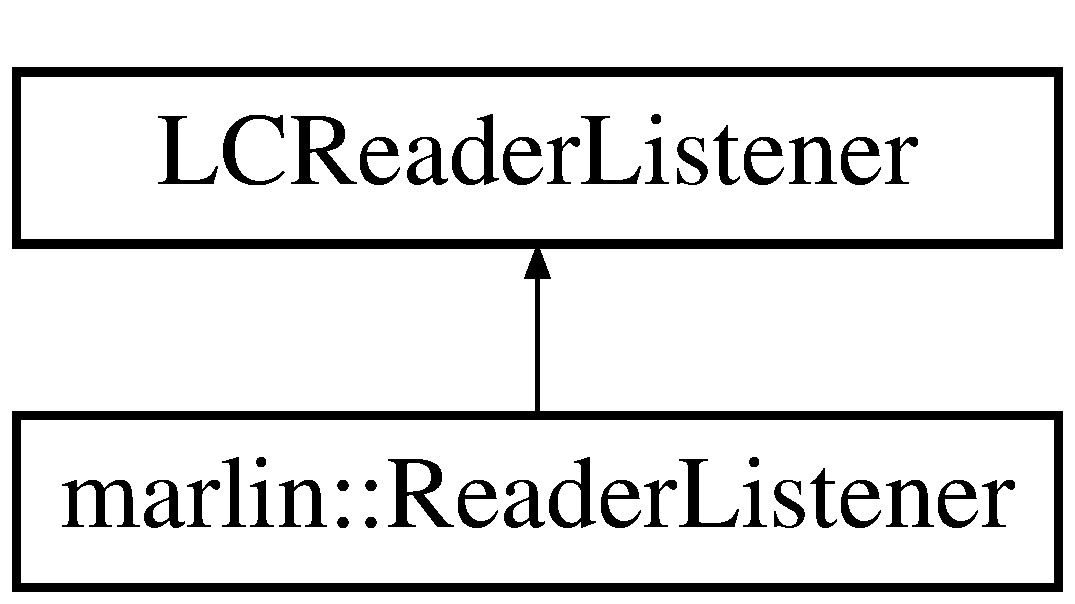
\includegraphics[height=2.000000cm]{classmarlin_1_1ReaderListener}
\end{center}
\end{figure}
\subsection*{Public Types}
\begin{DoxyCompactItemize}
\item 
\mbox{\label{classmarlin_1_1ReaderListener_a857d2b6a80908fd596cbe00e07402a1e}} 
using {\bfseries L\+C\+Event\+Function} = std\+::function$<$ void(std\+::shared\+\_\+ptr$<$ E\+V\+E\+N\+T\+::\+L\+C\+Event $>$)$>$
\item 
\mbox{\label{classmarlin_1_1ReaderListener_a9af1bc36ada5f6de5cf7bf789f8bd494}} 
using {\bfseries L\+C\+Run\+Header\+Function} = std\+::function$<$ void(std\+::shared\+\_\+ptr$<$ E\+V\+E\+N\+T\+::\+L\+C\+Run\+Header $>$)$>$
\end{DoxyCompactItemize}
\subsection*{Public Member Functions}
\begin{DoxyCompactItemize}
\item 
\mbox{\label{classmarlin_1_1ReaderListener_a2610225dfe19116e5d19347212126107}} 
{\bfseries Reader\+Listener} (const \textbf{ Reader\+Listener} \&)=delete
\item 
\mbox{\label{classmarlin_1_1ReaderListener_aa9f04c2e461622dd9ef732c3aa3340e6}} 
\textbf{ Reader\+Listener} \& {\bfseries operator=} (const \textbf{ Reader\+Listener} \&)=delete
\item 
\mbox{\label{classmarlin_1_1ReaderListener_ace530543ac8e30ba782519400220c839}} 
void \textbf{ on\+Event\+Read} (L\+C\+Event\+Function func)
\begin{DoxyCompactList}\small\item\em Set the callback function to process on event read. \end{DoxyCompactList}\item 
\mbox{\label{classmarlin_1_1ReaderListener_a698ef3c845f2fea2e809abc276adce17}} 
void \textbf{ on\+Run\+Header\+Read} (L\+C\+Run\+Header\+Function func)
\begin{DoxyCompactList}\small\item\em Set the callback function to process on run header read. \end{DoxyCompactList}\end{DoxyCompactItemize}


\subsection{Detailed Description}
\doxyref{Reader\+Listener}{p.}{classmarlin_1_1ReaderListener} class. 

Simple implementation of a reader listener. Callback functions can be set using lambda function, std\+::function objects or resulting call of std\+::bind call.

Example with lambda functions\+: 
\begin{DoxyCode}
ReaderListener listener ;
listener.onEventRead( [](std::shared\_ptr<EVENT::LCEvent> event)\{
  std::cout << \textcolor{stringliteral}{"Read event no "} << \textcolor{keyword}{event}->getEventNumber() << std::endl ;
\}) ;
listener.onRunHeaderRead( [](std::shared\_ptr<EVENT::LCRunHeader> rhdr)\{
  std::cout << \textcolor{stringliteral}{"Read run header no "} << rhdr->getRunNumber() << std::endl ;
\}) ;
\end{DoxyCode}


Example with std\+::bind and custom class method\+: 
\begin{DoxyCode}
\textcolor{keyword}{using namespace }std::placeholders ;
UserClass user ;
ReaderListener listener ;
listener.onEventRead( std::bind(&UserClass::processEvent, &user, \_1) ) ;
listener.onRunHeaderRead( std::bind(&UserClass::processRunHeader, &user, \_1) ) ;
\end{DoxyCode}


Note that the current implementation forward the processing only on modify\+Event() and modify\+Run\+Header(). Thus the data can be modified in callback functions. This is a requirement for concurrent applications 

The documentation for this class was generated from the following files\+:\begin{DoxyCompactItemize}
\item 
Reader\+Listener.\+h\item 
Reader\+Listener.\+cc\end{DoxyCompactItemize}

\section{marlin\+:\+:Rewind\+Data\+Files\+Exception Class Reference}
\label{classmarlin_1_1RewindDataFilesException}\index{marlin\+::\+Rewind\+Data\+Files\+Exception@{marlin\+::\+Rewind\+Data\+Files\+Exception}}


\doxyref{Rewind\+Data\+Files\+Exception}{p.}{classmarlin_1_1RewindDataFilesException} used to stop the current proccessing of events, rewind to the first event and restart the processing.  




{\ttfamily \#include $<$Exceptions.\+h$>$}

Inheritance diagram for marlin\+:\+:Rewind\+Data\+Files\+Exception\+:\begin{figure}[H]
\begin{center}
\leavevmode
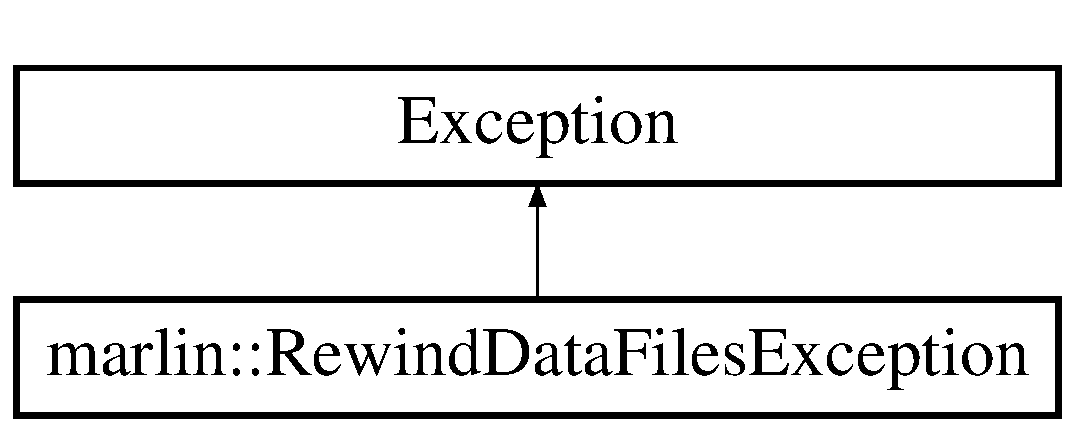
\includegraphics[height=2.000000cm]{classmarlin_1_1RewindDataFilesException}
\end{center}
\end{figure}
\subsection*{Public Member Functions}
\begin{DoxyCompactItemize}
\item 
\mbox{\label{classmarlin_1_1RewindDataFilesException_a2ae0dbe3e177f158b74a57fd0e4b0ab3}} 
{\bfseries Rewind\+Data\+Files\+Exception} (const \textbf{ Processor} $\ast$proc)
\end{DoxyCompactItemize}


\subsection{Detailed Description}
\doxyref{Rewind\+Data\+Files\+Exception}{p.}{classmarlin_1_1RewindDataFilesException} used to stop the current proccessing of events, rewind to the first event and restart the processing. 

\begin{DoxyAuthor}{Author}
gaede 
\end{DoxyAuthor}
\begin{DoxyVersion}{Version}

\end{DoxyVersion}
\begin{DoxyParagraph}{Id}
\doxyref{Exceptions.\+h}{p.}{Exceptions_8h_source},v 1.\+5 2007-\/02-\/02 17\+:15\+:25 gaede Exp 
\end{DoxyParagraph}


The documentation for this class was generated from the following files\+:\begin{DoxyCompactItemize}
\item 
Exceptions.\+h\item 
Exceptions.\+cc\end{DoxyCompactItemize}

\section{marlin\+:\+:Sequence Class Reference}
\label{classmarlin_1_1Sequence}\index{marlin\+::\+Sequence@{marlin\+::\+Sequence}}


\doxyref{Sequence}{p.}{classmarlin_1_1Sequence} class A sequence is a list of processors wrapped in \doxyref{Sequence\+Item}{p.}{classmarlin_1_1SequenceItem} objects.  




{\ttfamily \#include $<$Sequence.\+h$>$}

\subsection*{Public Types}
\begin{DoxyCompactItemize}
\item 
\mbox{\label{classmarlin_1_1Sequence_ad284349e00ff6756186069b4d6e104a6}} 
using {\bfseries Container} = std\+::vector$<$ std\+::shared\+\_\+ptr$<$ \textbf{ Sequence\+Item} $>$ $>$
\item 
\mbox{\label{classmarlin_1_1Sequence_a29a6610a7000468f2378ea9cb8cbe985}} 
using {\bfseries Index} = Container\+::size\+\_\+type
\item 
\mbox{\label{classmarlin_1_1Sequence_a5058e2c9c53f96d7a6fcbc163d42d07e}} 
using {\bfseries Size\+Type} = Container\+::size\+\_\+type
\item 
\mbox{\label{classmarlin_1_1Sequence_ac9a3014dbe4bb2a6341d3fb2de3c84e0}} 
using {\bfseries Clock\+Measure\+Map} = std\+::map$<$ std\+::string, \textbf{ Clock\+Measure} $>$
\item 
\mbox{\label{classmarlin_1_1Sequence_afab9d2c648de533c2c8fb31c094056a1}} 
using {\bfseries Skipped\+Event\+Map} = std\+::map$<$ std\+::string, int $>$
\end{DoxyCompactItemize}
\subsection*{Public Member Functions}
\begin{DoxyCompactItemize}
\item 
\mbox{\label{classmarlin_1_1Sequence_abcbec940e185b8cc340c44bb0ae0d689}} 
\textbf{ Sequence} \& {\bfseries operator=} (const \textbf{ Sequence} \&)=delete
\item 
\mbox{\label{classmarlin_1_1Sequence_ada7dc3933651a5c63a54c2344b699c55}} 
{\bfseries Sequence} (const \textbf{ Sequence} \&)=delete
\item 
std\+::shared\+\_\+ptr$<$ \textbf{ Sequence\+Item} $>$ \textbf{ create\+Item} (std\+::shared\+\_\+ptr$<$ \textbf{ Processor} $>$ processor, std\+::shared\+\_\+ptr$<$ std\+::mutex $>$ lock) const
\begin{DoxyCompactList}\small\item\em Create a sequence item. \end{DoxyCompactList}\item 
void \textbf{ add\+Item} (std\+::shared\+\_\+ptr$<$ \textbf{ Sequence\+Item} $>$ item)
\begin{DoxyCompactList}\small\item\em Add an item to the sequence. \end{DoxyCompactList}\item 
std\+::shared\+\_\+ptr$<$ \textbf{ Sequence\+Item} $>$ \textbf{ at} (Index index) const
\begin{DoxyCompactList}\small\item\em Get a sequence item at the specified index. \end{DoxyCompactList}\item 
\mbox{\label{classmarlin_1_1Sequence_a480a05e4e73728214b42d1292b3db905}} 
Size\+Type \textbf{ size} () const
\begin{DoxyCompactList}\small\item\em Get the number of items in the sequence. \end{DoxyCompactList}\item 
void \textbf{ process\+Run\+Header} (std\+::shared\+\_\+ptr$<$ E\+V\+E\+N\+T\+::\+L\+C\+Run\+Header $>$ rhdr)
\begin{DoxyCompactList}\small\item\em Process the run header. \end{DoxyCompactList}\item 
void \textbf{ modify\+Run\+Header} (std\+::shared\+\_\+ptr$<$ E\+V\+E\+N\+T\+::\+L\+C\+Run\+Header $>$ rhdr)
\begin{DoxyCompactList}\small\item\em Modify the run header. \end{DoxyCompactList}\item 
void \textbf{ process\+Event} (std\+::shared\+\_\+ptr$<$ E\+V\+E\+N\+T\+::\+L\+C\+Event $>$ event)
\begin{DoxyCompactList}\small\item\em Process the event. \end{DoxyCompactList}\item 
void \textbf{ modify\+Event} (std\+::shared\+\_\+ptr$<$ E\+V\+E\+N\+T\+::\+L\+C\+Event $>$ event)
\begin{DoxyCompactList}\small\item\em Modify the event. \end{DoxyCompactList}\item 
\mbox{\label{classmarlin_1_1Sequence_a1ed27674cb0ce1eb93b72414e656bc49}} 
\textbf{ Clock\+Measure} \textbf{ clock\+Measure\+Summary} () const
\begin{DoxyCompactList}\small\item\em Generate a clock measure summary of all items. \end{DoxyCompactList}\item 
\mbox{\label{classmarlin_1_1Sequence_aca5e6185c1994c4c481dcdb26d472843}} 
const Clock\+Measure\+Map \& \textbf{ clock\+Measures} () const
\begin{DoxyCompactList}\small\item\em Get all the clock measurements of the sequence. \end{DoxyCompactList}\item 
\mbox{\label{classmarlin_1_1Sequence_ab33aea0a5e6203004624a54bf3ef011f}} 
const Skipped\+Event\+Map \& \textbf{ skipped\+Events} () const
\begin{DoxyCompactList}\small\item\em Get all the skipped events of the sequence. \end{DoxyCompactList}\end{DoxyCompactItemize}


\subsection{Detailed Description}
\doxyref{Sequence}{p.}{classmarlin_1_1Sequence} class A sequence is a list of processors wrapped in \doxyref{Sequence\+Item}{p.}{classmarlin_1_1SequenceItem} objects. 

\doxyref{Sequence\+Item}{p.}{classmarlin_1_1SequenceItem} objects allow for calling processor methods in a critical section. This methods are \+:
\begin{DoxyItemize}
\item \doxyref{Processor\+::process\+Event()}{p.}{classmarlin_1_1Processor_a5bee49b5515f59fae755e0a26dfae91a}
\item Processor\+::modify\+Event()
\item \doxyref{Processor\+::process\+Run\+Header()}{p.}{classmarlin_1_1Processor_ab39f746a309bd096433a2bdaf3e75e43}
\item Processor\+::modify\+Run\+Header() \doxyref{Sequence}{p.}{classmarlin_1_1Sequence} provides a factory method \doxyref{create\+Item()}{p.}{classmarlin_1_1Sequence_a8949a36d64576cc91349f04530606377} to create items as shared pointer making it possible to share items between multiple sequence. To allow a proper management of multiple sequences in an application, see the \doxyref{Super\+Sequence}{p.}{classmarlin_1_1SuperSequence} class. 
\end{DoxyItemize}

\subsection{Member Function Documentation}
\mbox{\label{classmarlin_1_1Sequence_a60bb22e9f19d7a59fbc67bfb8cd183a2}} 
\index{marlin\+::\+Sequence@{marlin\+::\+Sequence}!add\+Item@{add\+Item}}
\index{add\+Item@{add\+Item}!marlin\+::\+Sequence@{marlin\+::\+Sequence}}
\subsubsection{add\+Item()}
{\footnotesize\ttfamily void marlin\+::\+Sequence\+::add\+Item (\begin{DoxyParamCaption}\item[{std\+::shared\+\_\+ptr$<$ \textbf{ Sequence\+Item} $>$}]{item }\end{DoxyParamCaption})}



Add an item to the sequence. 


\begin{DoxyParams}{Parameters}
{\em item} & the item to add \\
\hline
\end{DoxyParams}
\mbox{\label{classmarlin_1_1Sequence_ad875593c3c7f6d7c9b9c72ceeb6fb875}} 
\index{marlin\+::\+Sequence@{marlin\+::\+Sequence}!at@{at}}
\index{at@{at}!marlin\+::\+Sequence@{marlin\+::\+Sequence}}
\subsubsection{at()}
{\footnotesize\ttfamily std\+::shared\+\_\+ptr$<$ \textbf{ Sequence\+Item} $>$ marlin\+::\+Sequence\+::at (\begin{DoxyParamCaption}\item[{Index}]{index }\end{DoxyParamCaption}) const}



Get a sequence item at the specified index. 


\begin{DoxyParams}{Parameters}
{\em index} & the lookup index \\
\hline
\end{DoxyParams}
\mbox{\label{classmarlin_1_1Sequence_a8949a36d64576cc91349f04530606377}} 
\index{marlin\+::\+Sequence@{marlin\+::\+Sequence}!create\+Item@{create\+Item}}
\index{create\+Item@{create\+Item}!marlin\+::\+Sequence@{marlin\+::\+Sequence}}
\subsubsection{create\+Item()}
{\footnotesize\ttfamily std\+::shared\+\_\+ptr$<$ \textbf{ Sequence\+Item} $>$ marlin\+::\+Sequence\+::create\+Item (\begin{DoxyParamCaption}\item[{std\+::shared\+\_\+ptr$<$ \textbf{ Processor} $>$}]{processor,  }\item[{std\+::shared\+\_\+ptr$<$ std\+::mutex $>$}]{lock }\end{DoxyParamCaption}) const}



Create a sequence item. 

The item is not added. Use \doxyref{add\+Item()}{p.}{classmarlin_1_1Sequence_a60bb22e9f19d7a59fbc67bfb8cd183a2} to add it.


\begin{DoxyParams}{Parameters}
{\em processor} & a processor pointer \\
\hline
{\em lock} & the lock to use on process\+Event/modify\+Event calls \\
\hline
\end{DoxyParams}


References marlin\+::\+Sequence\+Item\+::processor().

\mbox{\label{classmarlin_1_1Sequence_af2f40f6a7b593fcc5117d97509b6766e}} 
\index{marlin\+::\+Sequence@{marlin\+::\+Sequence}!modify\+Event@{modify\+Event}}
\index{modify\+Event@{modify\+Event}!marlin\+::\+Sequence@{marlin\+::\+Sequence}}
\subsubsection{modify\+Event()}
{\footnotesize\ttfamily void marlin\+::\+Sequence\+::modify\+Event (\begin{DoxyParamCaption}\item[{std\+::shared\+\_\+ptr$<$ E\+V\+E\+N\+T\+::\+L\+C\+Event $>$}]{event }\end{DoxyParamCaption})}



Modify the event. 

Call \doxyref{modify\+Event()}{p.}{classmarlin_1_1Sequence_af2f40f6a7b593fcc5117d97509b6766e} for each item in the sequence


\begin{DoxyParams}{Parameters}
{\em event} & the event to modify \\
\hline
\end{DoxyParams}
\mbox{\label{classmarlin_1_1Sequence_a2fa5c1496f88725f7dd95dd7470c94dc}} 
\index{marlin\+::\+Sequence@{marlin\+::\+Sequence}!modify\+Run\+Header@{modify\+Run\+Header}}
\index{modify\+Run\+Header@{modify\+Run\+Header}!marlin\+::\+Sequence@{marlin\+::\+Sequence}}
\subsubsection{modify\+Run\+Header()}
{\footnotesize\ttfamily void marlin\+::\+Sequence\+::modify\+Run\+Header (\begin{DoxyParamCaption}\item[{std\+::shared\+\_\+ptr$<$ E\+V\+E\+N\+T\+::\+L\+C\+Run\+Header $>$}]{rhdr }\end{DoxyParamCaption})}



Modify the run header. 

Call \doxyref{modify\+Run\+Header()}{p.}{classmarlin_1_1Sequence_a2fa5c1496f88725f7dd95dd7470c94dc} for each item in the sequence


\begin{DoxyParams}{Parameters}
{\em rhdr} & the run header to modify \\
\hline
\end{DoxyParams}
\mbox{\label{classmarlin_1_1Sequence_a9e07975f81201d6dbecc99322d853bf6}} 
\index{marlin\+::\+Sequence@{marlin\+::\+Sequence}!process\+Event@{process\+Event}}
\index{process\+Event@{process\+Event}!marlin\+::\+Sequence@{marlin\+::\+Sequence}}
\subsubsection{process\+Event()}
{\footnotesize\ttfamily void marlin\+::\+Sequence\+::process\+Event (\begin{DoxyParamCaption}\item[{std\+::shared\+\_\+ptr$<$ E\+V\+E\+N\+T\+::\+L\+C\+Event $>$}]{event }\end{DoxyParamCaption})}



Process the event. 

Call \doxyref{process\+Event()}{p.}{classmarlin_1_1Sequence_a9e07975f81201d6dbecc99322d853bf6} for each item in the sequence


\begin{DoxyParams}{Parameters}
{\em event} & the event to process \\
\hline
\end{DoxyParams}
\mbox{\label{classmarlin_1_1Sequence_ab7a45b53c463d305a5d6017d65b9c911}} 
\index{marlin\+::\+Sequence@{marlin\+::\+Sequence}!process\+Run\+Header@{process\+Run\+Header}}
\index{process\+Run\+Header@{process\+Run\+Header}!marlin\+::\+Sequence@{marlin\+::\+Sequence}}
\subsubsection{process\+Run\+Header()}
{\footnotesize\ttfamily void marlin\+::\+Sequence\+::process\+Run\+Header (\begin{DoxyParamCaption}\item[{std\+::shared\+\_\+ptr$<$ E\+V\+E\+N\+T\+::\+L\+C\+Run\+Header $>$}]{rhdr }\end{DoxyParamCaption})}



Process the run header. 

Call \doxyref{process\+Run\+Header()}{p.}{classmarlin_1_1Sequence_ab7a45b53c463d305a5d6017d65b9c911} for each item in the sequence


\begin{DoxyParams}{Parameters}
{\em rhdr} & the run header to process \\
\hline
\end{DoxyParams}


The documentation for this class was generated from the following files\+:\begin{DoxyCompactItemize}
\item 
Sequence.\+h\item 
Sequence.\+cc\end{DoxyCompactItemize}

\section{marlin\+:\+:Sequence\+Item Class Reference}
\label{classmarlin_1_1SequenceItem}\index{marlin\+::\+Sequence\+Item@{marlin\+::\+Sequence\+Item}}


\doxyref{Sequence\+Item}{p.}{classmarlin_1_1SequenceItem} class Handle a processor pointer and call \doxyref{Processor\+::process\+Event}{p.}{classmarlin_1_1Processor_a5bee49b5515f59fae755e0a26dfae91a} in a critical section if configured accordingly.  




{\ttfamily \#include $<$Sequence.\+h$>$}

\subsection*{Public Member Functions}
\begin{DoxyCompactItemize}
\item 
\textbf{ Sequence\+Item} (std\+::shared\+\_\+ptr$<$ \textbf{ Processor} $>$ proc)
\begin{DoxyCompactList}\small\item\em Constructor. \end{DoxyCompactList}\item 
\textbf{ Sequence\+Item} (std\+::shared\+\_\+ptr$<$ \textbf{ Processor} $>$ proc, std\+::shared\+\_\+ptr$<$ std\+::mutex $>$ lock)
\begin{DoxyCompactList}\small\item\em Constructor. \end{DoxyCompactList}\item 
void \textbf{ process\+Run\+Header} (std\+::shared\+\_\+ptr$<$ E\+V\+E\+N\+T\+::\+L\+C\+Run\+Header $>$ rhdr)
\begin{DoxyCompactList}\small\item\em Process the run header. \end{DoxyCompactList}\item 
void \textbf{ modify\+Run\+Header} (std\+::shared\+\_\+ptr$<$ E\+V\+E\+N\+T\+::\+L\+C\+Run\+Header $>$ rhdr)
\begin{DoxyCompactList}\small\item\em Modify the run header. \end{DoxyCompactList}\item 
clock\+::pair \textbf{ process\+Event} (std\+::shared\+\_\+ptr$<$ E\+V\+E\+N\+T\+::\+L\+C\+Event $>$ event)
\begin{DoxyCompactList}\small\item\em Call \doxyref{Processor\+::process\+Event}{p.}{classmarlin_1_1Processor_a5bee49b5515f59fae755e0a26dfae91a}. \end{DoxyCompactList}\item 
clock\+::pair \textbf{ modify\+Event} (std\+::shared\+\_\+ptr$<$ E\+V\+E\+N\+T\+::\+L\+C\+Event $>$ event)
\begin{DoxyCompactList}\small\item\em Call Processor\+::modify\+Event. \end{DoxyCompactList}\item 
\mbox{\label{classmarlin_1_1SequenceItem_a00896e5cebd046c7137b2aa9a121efc7}} 
std\+::shared\+\_\+ptr$<$ \textbf{ Processor} $>$ \textbf{ processor} () const
\begin{DoxyCompactList}\small\item\em Get the processor instance. \end{DoxyCompactList}\item 
\mbox{\label{classmarlin_1_1SequenceItem_aeb3b15f63bfe8acbb71cc400bf75f0f1}} 
const std\+::string \& \textbf{ name} () const
\begin{DoxyCompactList}\small\item\em Get the processor name. \end{DoxyCompactList}\end{DoxyCompactItemize}


\subsection{Detailed Description}
\doxyref{Sequence\+Item}{p.}{classmarlin_1_1SequenceItem} class Handle a processor pointer and call \doxyref{Processor\+::process\+Event}{p.}{classmarlin_1_1Processor_a5bee49b5515f59fae755e0a26dfae91a} in a critical section if configured accordingly. 

\subsection{Constructor \& Destructor Documentation}
\mbox{\label{classmarlin_1_1SequenceItem_a2f100e16f21b318d9ffc2d320e7716a5}} 
\index{marlin\+::\+Sequence\+Item@{marlin\+::\+Sequence\+Item}!Sequence\+Item@{Sequence\+Item}}
\index{Sequence\+Item@{Sequence\+Item}!marlin\+::\+Sequence\+Item@{marlin\+::\+Sequence\+Item}}
\subsubsection{Sequence\+Item()\hspace{0.1cm}{\footnotesize\ttfamily [1/2]}}
{\footnotesize\ttfamily marlin\+::\+Sequence\+Item\+::\+Sequence\+Item (\begin{DoxyParamCaption}\item[{std\+::shared\+\_\+ptr$<$ \textbf{ Processor} $>$}]{proc }\end{DoxyParamCaption})}



Constructor. 

No internal locking


\begin{DoxyParams}{Parameters}
{\em proc} & a pointer on a processor \\
\hline
\end{DoxyParams}
\mbox{\label{classmarlin_1_1SequenceItem_a7c7e4b1ad94d1edae194ea9ae94c1674}} 
\index{marlin\+::\+Sequence\+Item@{marlin\+::\+Sequence\+Item}!Sequence\+Item@{Sequence\+Item}}
\index{Sequence\+Item@{Sequence\+Item}!marlin\+::\+Sequence\+Item@{marlin\+::\+Sequence\+Item}}
\subsubsection{Sequence\+Item()\hspace{0.1cm}{\footnotesize\ttfamily [2/2]}}
{\footnotesize\ttfamily marlin\+::\+Sequence\+Item\+::\+Sequence\+Item (\begin{DoxyParamCaption}\item[{std\+::shared\+\_\+ptr$<$ \textbf{ Processor} $>$}]{proc,  }\item[{std\+::shared\+\_\+ptr$<$ std\+::mutex $>$}]{lock }\end{DoxyParamCaption})}



Constructor. 


\begin{DoxyParams}{Parameters}
{\em proc} & a pointer on a processor \\
\hline
{\em lock} & the mutex instance to use \\
\hline
\end{DoxyParams}


\subsection{Member Function Documentation}
\mbox{\label{classmarlin_1_1SequenceItem_ad71887fc8401eb52b95597c1c9fd42f6}} 
\index{marlin\+::\+Sequence\+Item@{marlin\+::\+Sequence\+Item}!modify\+Event@{modify\+Event}}
\index{modify\+Event@{modify\+Event}!marlin\+::\+Sequence\+Item@{marlin\+::\+Sequence\+Item}}
\subsubsection{modify\+Event()}
{\footnotesize\ttfamily clock\+::pair marlin\+::\+Sequence\+Item\+::modify\+Event (\begin{DoxyParamCaption}\item[{std\+::shared\+\_\+ptr$<$ E\+V\+E\+N\+T\+::\+L\+C\+Event $>$}]{event }\end{DoxyParamCaption})}



Call Processor\+::modify\+Event. 

Lock if the mutex has been initialized Call time is returned in a pair as \+:
\begin{DoxyItemize}
\item first \+: the total time taking into account the mutex waiting time
\item second \+: the time spent on process event only
\end{DoxyItemize}


\begin{DoxyParams}{Parameters}
{\em event} & the event to modify \\
\hline
\end{DoxyParams}


References marlin\+::clock\+::now().

\mbox{\label{classmarlin_1_1SequenceItem_ab211f8a85cd5905c8e3be35872602c88}} 
\index{marlin\+::\+Sequence\+Item@{marlin\+::\+Sequence\+Item}!modify\+Run\+Header@{modify\+Run\+Header}}
\index{modify\+Run\+Header@{modify\+Run\+Header}!marlin\+::\+Sequence\+Item@{marlin\+::\+Sequence\+Item}}
\subsubsection{modify\+Run\+Header()}
{\footnotesize\ttfamily void marlin\+::\+Sequence\+Item\+::modify\+Run\+Header (\begin{DoxyParamCaption}\item[{std\+::shared\+\_\+ptr$<$ E\+V\+E\+N\+T\+::\+L\+C\+Run\+Header $>$}]{rhdr }\end{DoxyParamCaption})}



Modify the run header. 


\begin{DoxyParams}{Parameters}
{\em rhdr} & the run header to modify \\
\hline
\end{DoxyParams}
\mbox{\label{classmarlin_1_1SequenceItem_ac63897089f19002476453da272225823}} 
\index{marlin\+::\+Sequence\+Item@{marlin\+::\+Sequence\+Item}!process\+Event@{process\+Event}}
\index{process\+Event@{process\+Event}!marlin\+::\+Sequence\+Item@{marlin\+::\+Sequence\+Item}}
\subsubsection{process\+Event()}
{\footnotesize\ttfamily clock\+::pair marlin\+::\+Sequence\+Item\+::process\+Event (\begin{DoxyParamCaption}\item[{std\+::shared\+\_\+ptr$<$ E\+V\+E\+N\+T\+::\+L\+C\+Event $>$}]{event }\end{DoxyParamCaption})}



Call \doxyref{Processor\+::process\+Event}{p.}{classmarlin_1_1Processor_a5bee49b5515f59fae755e0a26dfae91a}. 

Lock if the mutex has been initialized. Call time is returned in a pair as \+:
\begin{DoxyItemize}
\item first \+: the total time taking into account the mutex waiting time
\item second \+: the time spent on process event only
\end{DoxyItemize}


\begin{DoxyParams}{Parameters}
{\em event} & the event to process \\
\hline
\end{DoxyParams}


References marlin\+::clock\+::now().

\mbox{\label{classmarlin_1_1SequenceItem_a9ddb5dc973eeb86cba79bada59c75abc}} 
\index{marlin\+::\+Sequence\+Item@{marlin\+::\+Sequence\+Item}!process\+Run\+Header@{process\+Run\+Header}}
\index{process\+Run\+Header@{process\+Run\+Header}!marlin\+::\+Sequence\+Item@{marlin\+::\+Sequence\+Item}}
\subsubsection{process\+Run\+Header()}
{\footnotesize\ttfamily void marlin\+::\+Sequence\+Item\+::process\+Run\+Header (\begin{DoxyParamCaption}\item[{std\+::shared\+\_\+ptr$<$ E\+V\+E\+N\+T\+::\+L\+C\+Run\+Header $>$}]{rhdr }\end{DoxyParamCaption})}



Process the run header. 


\begin{DoxyParams}{Parameters}
{\em rhdr} & the run header to process \\
\hline
\end{DoxyParams}


The documentation for this class was generated from the following files\+:\begin{DoxyCompactItemize}
\item 
Sequence.\+h\item 
Sequence.\+cc\end{DoxyCompactItemize}

\section{marlin\+:\+:Simple\+Cluster\+Smearer Class Reference}
\label{classmarlin_1_1SimpleClusterSmearer}\index{marlin\+::\+Simple\+Cluster\+Smearer@{marlin\+::\+Simple\+Cluster\+Smearer}}


Smears the four vectors of (neutral) clusters according to d\+E/E = A \char`\"{}+\char`\"{} B / sqrt( E/\+GeV ) for a given range of the polar angle.  




{\ttfamily \#include $<$Simple\+Cluster\+Smearer.\+h$>$}

Inheritance diagram for marlin\+:\+:Simple\+Cluster\+Smearer\+:\begin{figure}[H]
\begin{center}
\leavevmode
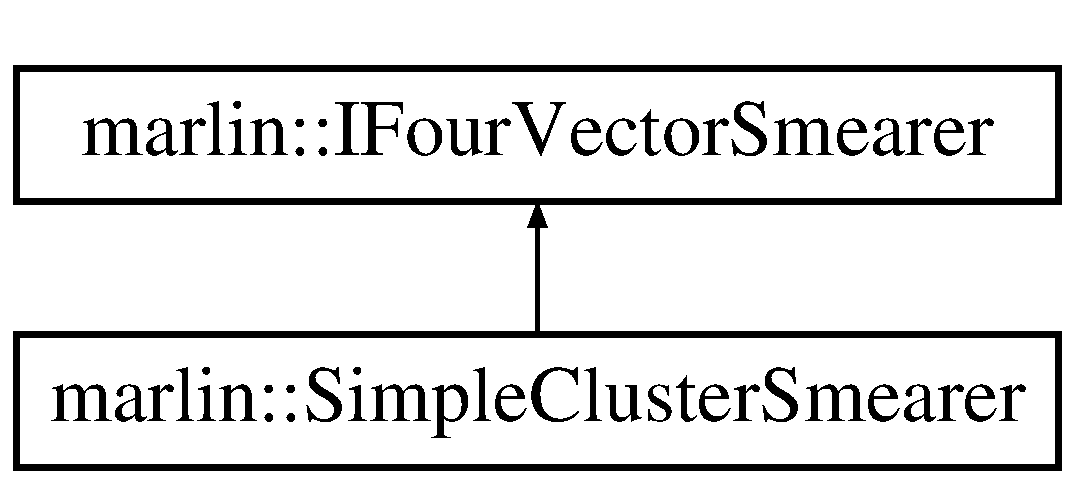
\includegraphics[height=2.000000cm]{classmarlin_1_1SimpleClusterSmearer}
\end{center}
\end{figure}
\subsection*{Public Member Functions}
\begin{DoxyCompactItemize}
\item 
\mbox{\label{classmarlin_1_1SimpleClusterSmearer_a1b1449168817bbb42ba93e6c1d5e5297}} 
{\bfseries Simple\+Cluster\+Smearer} (const std\+::vector$<$ float $>$ \&res\+Vec)
\item 
virtual \textbf{ $\sim$\+Simple\+Cluster\+Smearer} ()
\begin{DoxyCompactList}\small\item\em Virtual d\textquotesingle{}tor. \end{DoxyCompactList}\item 
virtual Hep\+Lorentz\+Vector \textbf{ smeared\+Four\+Vector} (const Hep\+Lorentz\+Vector \&v, int pdg\+Code)
\begin{DoxyCompactList}\small\item\em Smears the given four vector according to the resolution for the polar angle of the cluster. \end{DoxyCompactList}\end{DoxyCompactItemize}
\subsection*{Protected Attributes}
\begin{DoxyCompactItemize}
\item 
\mbox{\label{classmarlin_1_1SimpleClusterSmearer_aab7dbe0afca58835a2be6942a0c3d37f}} 
Res\+Vec {\bfseries \+\_\+res\+Vec}
\end{DoxyCompactItemize}


\subsection{Detailed Description}
Smears the four vectors of (neutral) clusters according to d\+E/E = A \char`\"{}+\char`\"{} B / sqrt( E/\+GeV ) for a given range of the polar angle. 

The resolution parameters A and B are given in the constructor as a vector holding quadruples of\+: A0, B0, th\+\_\+min0, th\+\_\+max0, A0, B0, th\+\_\+min1, th\+\_\+max1, ...~\newline
 Momenta are assigned assumig massless particles. 

\subsection{Constructor \& Destructor Documentation}
\mbox{\label{classmarlin_1_1SimpleClusterSmearer_a7eec35bfde7e3cc856351555f0045c4e}} 
\index{marlin\+::\+Simple\+Cluster\+Smearer@{marlin\+::\+Simple\+Cluster\+Smearer}!````~Simple\+Cluster\+Smearer@{$\sim$\+Simple\+Cluster\+Smearer}}
\index{````~Simple\+Cluster\+Smearer@{$\sim$\+Simple\+Cluster\+Smearer}!marlin\+::\+Simple\+Cluster\+Smearer@{marlin\+::\+Simple\+Cluster\+Smearer}}
\subsubsection{$\sim$\+Simple\+Cluster\+Smearer()}
{\footnotesize\ttfamily virtual marlin\+::\+Simple\+Cluster\+Smearer\+::$\sim$\+Simple\+Cluster\+Smearer (\begin{DoxyParamCaption}{ }\end{DoxyParamCaption})\hspace{0.3cm}{\ttfamily [inline]}, {\ttfamily [virtual]}}



Virtual d\textquotesingle{}tor. 



\subsection{Member Function Documentation}
\mbox{\label{classmarlin_1_1SimpleClusterSmearer_a99b596644eccdb5380976fde0d49bd45}} 
\index{marlin\+::\+Simple\+Cluster\+Smearer@{marlin\+::\+Simple\+Cluster\+Smearer}!smeared\+Four\+Vector@{smeared\+Four\+Vector}}
\index{smeared\+Four\+Vector@{smeared\+Four\+Vector}!marlin\+::\+Simple\+Cluster\+Smearer@{marlin\+::\+Simple\+Cluster\+Smearer}}
\subsubsection{smeared\+Four\+Vector()}
{\footnotesize\ttfamily Hep\+Lorentz\+Vector marlin\+::\+Simple\+Cluster\+Smearer\+::smeared\+Four\+Vector (\begin{DoxyParamCaption}\item[{const Hep\+Lorentz\+Vector \&}]{v,  }\item[{int}]{pdg\+Code }\end{DoxyParamCaption})\hspace{0.3cm}{\ttfamily [virtual]}}



Smears the given four vector according to the resolution for the polar angle of the cluster. 

Returns a vector with all elements 0. if no resolution is defined. 

Implements \textbf{ marlin\+::\+I\+Four\+Vector\+Smearer} \doxyref{}{p.}{classmarlin_1_1IFourVectorSmearer_a69a3ece59f66350310e1eb1c696464ce}.



The documentation for this class was generated from the following files\+:\begin{DoxyCompactItemize}
\item 
Simple\+Cluster\+Smearer.\+h\item 
Simple\+Cluster\+Smearer.\+cc\end{DoxyCompactItemize}

\section{marlin\+:\+:Simple\+Fast\+M\+C\+Processor Class Reference}
\label{classmarlin_1_1SimpleFastMCProcessor}\index{marlin\+::\+Simple\+Fast\+M\+C\+Processor@{marlin\+::\+Simple\+Fast\+M\+C\+Processor}}


A simple smearing \char`\"{}\+Monte Carlo\char`\"{} processor.  


Inheritance diagram for marlin\+:\+:Simple\+Fast\+M\+C\+Processor\+:\begin{figure}[H]
\begin{center}
\leavevmode
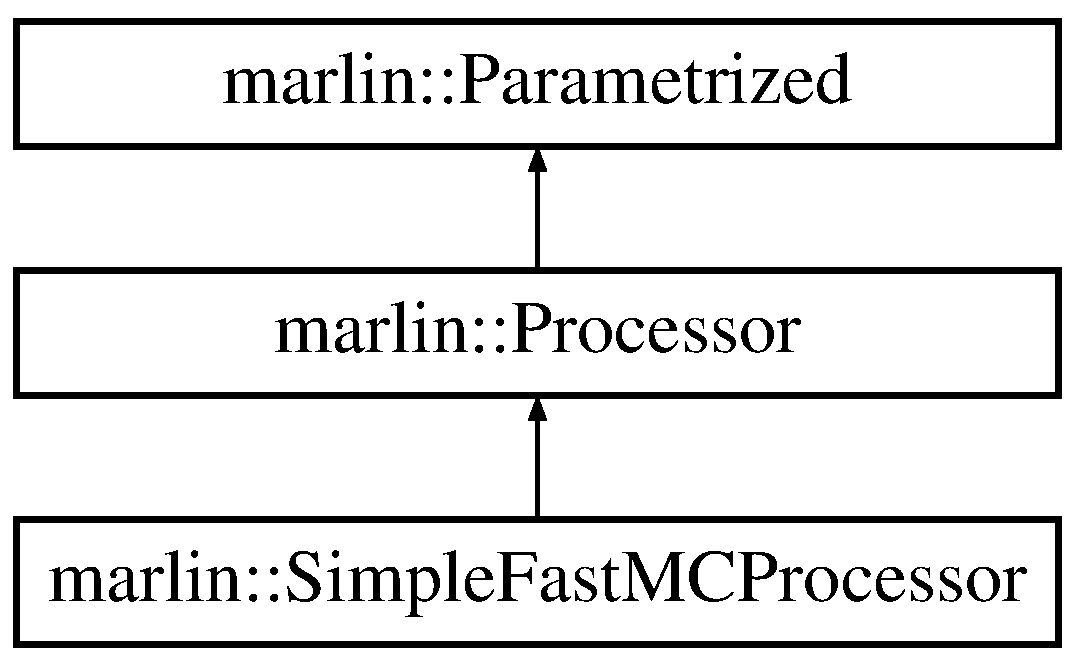
\includegraphics[height=3.000000cm]{classmarlin_1_1SimpleFastMCProcessor}
\end{center}
\end{figure}
\subsection*{Public Member Functions}
\begin{DoxyCompactItemize}
\item 
\mbox{\label{classmarlin_1_1SimpleFastMCProcessor_a47cc7c8344ae0be24d621f311d4c7ac1}} 
{\bfseries Simple\+Fast\+M\+C\+Processor} (const \textbf{ marlin\+::\+Simple\+Fast\+M\+C\+Processor} \&)=delete
\item 
\mbox{\label{classmarlin_1_1SimpleFastMCProcessor_a3bb3441abbab4edc7df6f10b36aa3579}} 
\textbf{ Simple\+Fast\+M\+C\+Processor} \& {\bfseries operator=} (const \textbf{ marlin\+::\+Simple\+Fast\+M\+C\+Processor} \&)=delete
\item 
\mbox{\label{classmarlin_1_1SimpleFastMCProcessor_a7d5ba5c7f2d639b0d15d1d61e45fd2a9}} 
\textbf{ Processor} $\ast$ \textbf{ new\+Processor} ()
\begin{DoxyCompactList}\small\item\em Return a new instance of the processor (factory method) \end{DoxyCompactList}\item 
void \textbf{ init} ()
\begin{DoxyCompactList}\small\item\em Initialize the processor. \end{DoxyCompactList}\item 
void \textbf{ process\+Event} (E\+V\+E\+N\+T\+::\+L\+C\+Event $\ast$evt)
\begin{DoxyCompactList}\small\item\em Process an input event. \end{DoxyCompactList}\end{DoxyCompactItemize}
\subsection*{Additional Inherited Members}


\subsection{Detailed Description}
A simple smearing \char`\"{}\+Monte Carlo\char`\"{} processor. 

It creates Reconstructed\+Particles from M\+C\+Particles according to the resolution that is specified for the particle type, one of\+: 
\begin{DoxyItemize}
\item photon 
\item charged\+: e+-\/,mu+-\/,pi+-\/,K+-\/,p+-\/,.... 
\item neutral hadron\+: K0L, n, Lambda0,... 
\end{DoxyItemize}The resolutions for charged particles are given as delta(1/P) for a certain polar angle range (mapped to [0.,pi/2.]), e.\+g. ~\newline
 {\bfseries Charged\+Resolution ~ .7e-\/5 ~ 0. ~ 3.\+141593/2. }~\newline
 sets the resolution for all charged particles to 0.\+7$\ast$10$^\wedge$-\/5.~\newline
 Specifying different resolutions for different polar angle ranges allows to mimic degrading detector performance in the very forward region. ~\newline
 The energy of the charged Reconstructed\+Particles is set from the \char`\"{}measured\char`\"{} momentum using the energy momentum relation for electrons and muons and assuming the pion mass for all other charged tracks.~\newline
 The resolutions for neutral particles are given as A and B for a certain polar angle range, where d\+E/E = A \char`\"{}+\char`\"{} B / sqrt(E/\+GeV), e.\+g. ~\newline
 {\bfseries Neutral\+Hadron\+Resolution ~ 0.\+03 ~ .30 ~ 0. ~ 3.\+141593/2. }~\newline
 sets the resolution for all neutral hadrons to 3\% \char`\"{}+\char`\"{} 30\% / sqrt( E /\+GeV ). The resolution for gammas is specified in {\bfseries Photon\+Resolution}~\newline
 No Reconstructed\+Particles are created if there is no resolution defined at that polar angle, e.\+g.~\newline
 {\bfseries Photon\+Resolution ~ .7e-\/5 ~ 0.\+083 ~ 3.\+141593/2. }~\newline
 effectively limits the acceptance region for photons to theta $>$ 83mrad.~\newline


A collection of L\+C\+Relations, called \char`\"{}\+M\+C\+Truth\+Mapping\char`\"{} holds the relation between the Reconstructed\+Particles and their proper M\+C\+Particles.

\subparagraph*{Input -\/ Prerequisites}

A collection of M\+C\+Particles (the M\+C\+P\+Article collection).

\subparagraph*{Output}


\begin{DoxyItemize}
\item {\bfseries Reconstructed\+Particles}\+: the collection of reconstructed particles 
\item {\bfseries M\+C\+Truth\+Mapping}\+: holds L\+C\+Relations that map the Reconstructed\+Particles to their proper M\+C\+Particles  
\end{DoxyItemize}


\begin{DoxyParams}{Parameters}
{\em Charged\+Resolution} & Resolution of charged particles in polar angle range\+: d(1/P) th\+\_\+min th\+\_\+max \\
\hline
{\em Input\+Collection\+Name} & Name of the M\+C\+Particle input collection \\
\hline
{\em Momentum\+Cut} & No reconstructed particles are produced for smaller momenta (in [GeV]) \\
\hline
{\em Neutral\+Hadron\+Resolution} & Resolution d\+E/E=A+\+B/sqrt(E/\+GeV) of neutral hadrons in polar angle range\+: A B th\+\_\+min th\+\_\+max \\
\hline
{\em Photon\+Resolution} & Resolution d\+E/E=A+\+B/sqrt(E/\+GeV) of photons in polar angle range\+: A B th\+\_\+min th\+\_\+max\\
\hline
{\em Reco\+Particle\+Collection\+Name} & default is \char`\"{}\+Reconstructed\+Particles\char`\"{} \\
\hline
{\em M\+C\+Truth\+Mapping\+Collection\+Name} & default is \char`\"{}\+M\+C\+Truth\+Mapping\char`\"{}\\
\hline
\end{DoxyParams}
\begin{DoxyAuthor}{Author}
F. Gaede, D\+E\+SY 
\end{DoxyAuthor}
\begin{DoxyVersion}{Version}

\end{DoxyVersion}
\begin{DoxyParagraph}{Id}
Simple\+Fast\+M\+C\+Processor.\+h,v 1.\+4 2007-\/07-\/04 12\+:13\+:06 gaede Exp 
\end{DoxyParagraph}


\subsection{Member Function Documentation}
\mbox{\label{classmarlin_1_1SimpleFastMCProcessor_aea0d8a3a1bde4211398554449ba61e34}} 
\index{marlin\+::\+Simple\+Fast\+M\+C\+Processor@{marlin\+::\+Simple\+Fast\+M\+C\+Processor}!init@{init}}
\index{init@{init}!marlin\+::\+Simple\+Fast\+M\+C\+Processor@{marlin\+::\+Simple\+Fast\+M\+C\+Processor}}
\subsubsection{init()}
{\footnotesize\ttfamily void marlin\+::\+Simple\+Fast\+M\+C\+Processor\+::init (\begin{DoxyParamCaption}{ }\end{DoxyParamCaption})\hspace{0.3cm}{\ttfamily [virtual]}}



Initialize the processor. 

Called at the begin of the job before anything is read. Use to initialize the processor, e.\+g. book histograms. 

Reimplemented from \textbf{ marlin\+::\+Processor} \doxyref{}{p.}{classmarlin_1_1Processor_a8194fb92a428de40ea9d891c8c8aed6b}.



References marlin\+::\+Processor\+::print\+Parameters(), marlin\+::\+Simple\+Particle\+Factory\+::register\+I\+Four\+Vector\+Smearer(), and marlin\+::\+Simple\+Particle\+Factory\+::set\+Momentum\+Cut().

\mbox{\label{classmarlin_1_1SimpleFastMCProcessor_aa4c8ea6b05fd5620870b527589098f20}} 
\index{marlin\+::\+Simple\+Fast\+M\+C\+Processor@{marlin\+::\+Simple\+Fast\+M\+C\+Processor}!process\+Event@{process\+Event}}
\index{process\+Event@{process\+Event}!marlin\+::\+Simple\+Fast\+M\+C\+Processor@{marlin\+::\+Simple\+Fast\+M\+C\+Processor}}
\subsubsection{process\+Event()}
{\footnotesize\ttfamily void marlin\+::\+Simple\+Fast\+M\+C\+Processor\+::process\+Event (\begin{DoxyParamCaption}\item[{E\+V\+E\+N\+T\+::\+L\+C\+Event $\ast$}]{ }\end{DoxyParamCaption})\hspace{0.3cm}{\ttfamily [virtual]}}



Process an input event. 

Called for every event -\/ the working horse. 

Reimplemented from \textbf{ marlin\+::\+Processor} \doxyref{}{p.}{classmarlin_1_1Processor_a5bee49b5515f59fae755e0a26dfae91a}.



References marlin\+::\+I\+Reco\+Particle\+Factory\+::create\+Reconstructed\+Particle().



The documentation for this class was generated from the following file\+:\begin{DoxyCompactItemize}
\item 
Simple\+Fast\+M\+C\+Processor.\+cc\end{DoxyCompactItemize}

\section{marlin\+:\+:Simple\+Particle\+Factory Class Reference}
\label{classmarlin_1_1SimpleParticleFactory}\index{marlin\+::\+Simple\+Particle\+Factory@{marlin\+::\+Simple\+Particle\+Factory}}


Implementation of \doxyref{I\+Reco\+Particle\+Factory}{p.}{classmarlin_1_1IRecoParticleFactory} that implements the default behaviour as described in \doxyref{Simple\+Fast\+M\+C\+Processor}{p.}{classmarlin_1_1SimpleFastMCProcessor}, i.\+e.  




{\ttfamily \#include $<$Simple\+Particle\+Factory.\+h$>$}

Inheritance diagram for marlin\+:\+:Simple\+Particle\+Factory\+:\begin{figure}[H]
\begin{center}
\leavevmode
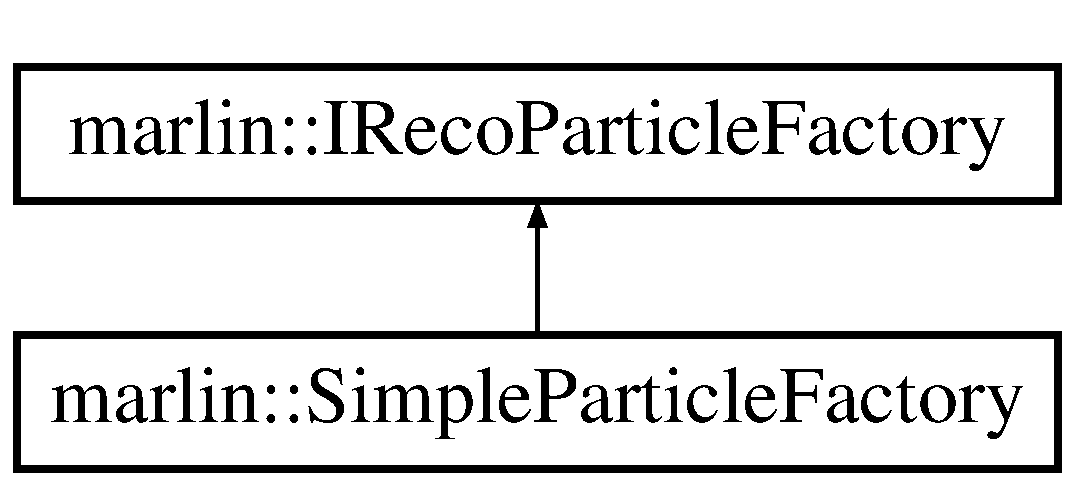
\includegraphics[height=2.000000cm]{classmarlin_1_1SimpleParticleFactory}
\end{center}
\end{figure}
\subsection*{Public Member Functions}
\begin{DoxyCompactItemize}
\item 
virtual \textbf{ $\sim$\+Simple\+Particle\+Factory} ()
\begin{DoxyCompactList}\small\item\em Virtual d\textquotesingle{}tor. \end{DoxyCompactList}\item 
\mbox{\label{classmarlin_1_1SimpleParticleFactory_a2c050bb3a0c06aadcb5ef9c552b409f7}} 
virtual lcio\+::\+Reconstructed\+Particle $\ast$ \textbf{ create\+Reconstructed\+Particle} (const lcio\+::\+M\+C\+Particle $\ast$mcp)
\begin{DoxyCompactList}\small\item\em The actual factory method that creates a new Reconstructed\+Particle. \end{DoxyCompactList}\item 
\mbox{\label{classmarlin_1_1SimpleParticleFactory_a3f82779ebc96a54c59433f914f6eb62c}} 
virtual void \textbf{ register\+I\+Four\+Vector\+Smearer} (\textbf{ I\+Four\+Vector\+Smearer} $\ast$sm, Fast\+M\+C\+Particle\+Type type)
\begin{DoxyCompactList}\small\item\em Register a particle four vector smearer for the given type. \end{DoxyCompactList}\item 
\mbox{\label{classmarlin_1_1SimpleParticleFactory_ac0fd79c9ba9d28f8108fca9fd96cdaee}} 
virtual Fast\+M\+C\+Particle\+Type \textbf{ get\+Particle\+Type} (const lcio\+::\+M\+C\+Particle $\ast$mcp)
\begin{DoxyCompactList}\small\item\em Returns the type of the M\+C\+Particle. \end{DoxyCompactList}\item 
virtual void \textbf{ set\+Momentum\+Cut} (double m\+Cut)
\begin{DoxyCompactList}\small\item\em Helper function to determine the charge from the P\+DG (charge is missing from stdhep files) \end{DoxyCompactList}\end{DoxyCompactItemize}
\subsection*{Protected Attributes}
\begin{DoxyCompactItemize}
\item 
\mbox{\label{classmarlin_1_1SimpleParticleFactory_aa5e09f4fca0e2746028e76f5eed82df1}} 
std\+::vector$<$ \textbf{ I\+Four\+Vector\+Smearer} $\ast$ $>$ {\bfseries \+\_\+smearing\+Vec}
\item 
\mbox{\label{classmarlin_1_1SimpleParticleFactory_a14a673f3e4ec54a13a465f53f93d3f0c}} 
double {\bfseries \+\_\+momentum\+Cut}
\end{DoxyCompactItemize}


\subsection{Detailed Description}
Implementation of \doxyref{I\+Reco\+Particle\+Factory}{p.}{classmarlin_1_1IRecoParticleFactory} that implements the default behaviour as described in \doxyref{Simple\+Fast\+M\+C\+Processor}{p.}{classmarlin_1_1SimpleFastMCProcessor}, i.\+e. 

have polar angle ranges with different resolutions for charged tracks, photons and neutral hadrons.

\begin{DoxyAuthor}{Author}
F. Gaede, D\+E\+SY 
\end{DoxyAuthor}
\begin{DoxyVersion}{Version}

\end{DoxyVersion}
\begin{DoxyParagraph}{Id}
\doxyref{Simple\+Particle\+Factory.\+h}{p.}{SimpleParticleFactory_8h_source},v 1.\+3 2007-\/11-\/23 20\+:09\+:12 gaede Exp 
\end{DoxyParagraph}


\subsection{Constructor \& Destructor Documentation}
\mbox{\label{classmarlin_1_1SimpleParticleFactory_a5ed083943b298f870fd2caf91a139108}} 
\index{marlin\+::\+Simple\+Particle\+Factory@{marlin\+::\+Simple\+Particle\+Factory}!````~Simple\+Particle\+Factory@{$\sim$\+Simple\+Particle\+Factory}}
\index{````~Simple\+Particle\+Factory@{$\sim$\+Simple\+Particle\+Factory}!marlin\+::\+Simple\+Particle\+Factory@{marlin\+::\+Simple\+Particle\+Factory}}
\subsubsection{$\sim$\+Simple\+Particle\+Factory()}
{\footnotesize\ttfamily virtual marlin\+::\+Simple\+Particle\+Factory\+::$\sim$\+Simple\+Particle\+Factory (\begin{DoxyParamCaption}{ }\end{DoxyParamCaption})\hspace{0.3cm}{\ttfamily [inline]}, {\ttfamily [virtual]}}



Virtual d\textquotesingle{}tor. 



References create\+Reconstructed\+Particle(), get\+Particle\+Type(), register\+I\+Four\+Vector\+Smearer(), and set\+Momentum\+Cut().



\subsection{Member Function Documentation}
\mbox{\label{classmarlin_1_1SimpleParticleFactory_a026d4533ca033bbf85a02341933a2dc9}} 
\index{marlin\+::\+Simple\+Particle\+Factory@{marlin\+::\+Simple\+Particle\+Factory}!set\+Momentum\+Cut@{set\+Momentum\+Cut}}
\index{set\+Momentum\+Cut@{set\+Momentum\+Cut}!marlin\+::\+Simple\+Particle\+Factory@{marlin\+::\+Simple\+Particle\+Factory}}
\subsubsection{set\+Momentum\+Cut()}
{\footnotesize\ttfamily void marlin\+::\+Simple\+Particle\+Factory\+::set\+Momentum\+Cut (\begin{DoxyParamCaption}\item[{double}]{m\+Cut }\end{DoxyParamCaption})\hspace{0.3cm}{\ttfamily [virtual]}}



Helper function to determine the charge from the P\+DG (charge is missing from stdhep files) 

Set the momentum cut in GeV -\/ no particles are produced for ower momenta. Default is 0.\+1 eV. 

Referenced by marlin\+::\+Simple\+Fast\+M\+C\+Processor\+::init(), and $\sim$\+Simple\+Particle\+Factory().



The documentation for this class was generated from the following files\+:\begin{DoxyCompactItemize}
\item 
Simple\+Particle\+Factory.\+h\item 
Simple\+Particle\+Factory.\+cc\end{DoxyCompactItemize}

\section{marlin\+:\+:Simple\+Scheduler Class Reference}
\label{classmarlin_1_1SimpleScheduler}\index{marlin\+::\+Simple\+Scheduler@{marlin\+::\+Simple\+Scheduler}}


\doxyref{Simple\+Scheduler}{p.}{classmarlin_1_1SimpleScheduler} class.  




{\ttfamily \#include $<$Simple\+Scheduler.\+h$>$}

Inheritance diagram for marlin\+:\+:Simple\+Scheduler\+:\begin{figure}[H]
\begin{center}
\leavevmode
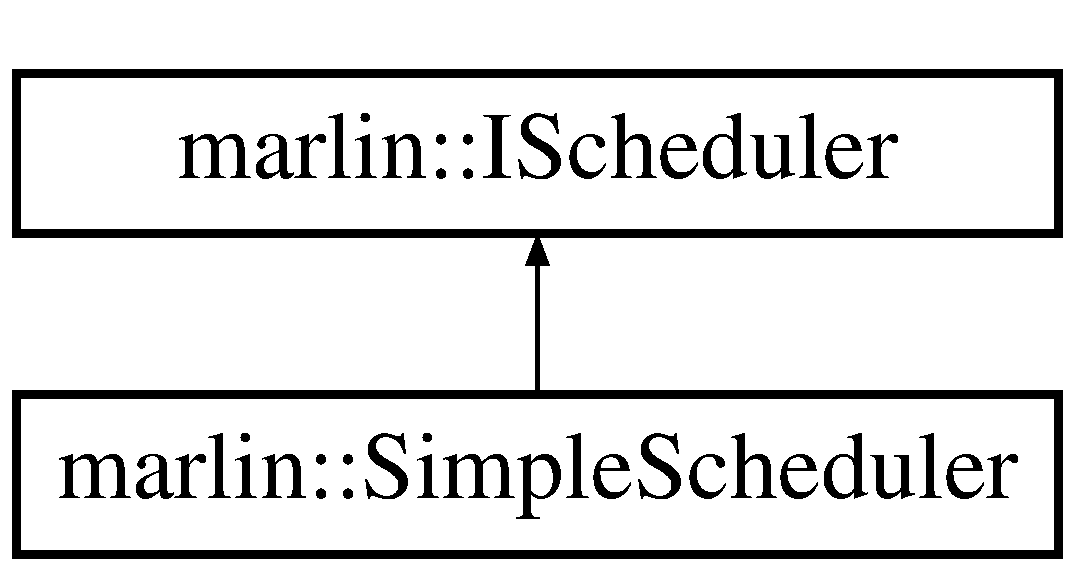
\includegraphics[height=2.000000cm]{classmarlin_1_1SimpleScheduler}
\end{center}
\end{figure}
\subsection*{Public Types}
\begin{DoxyCompactItemize}
\item 
\mbox{\label{classmarlin_1_1SimpleScheduler_a08f82cd32efe0cf8edf0eff0bd879b2c}} 
using {\bfseries Logger} = Logging\+::\+Logger
\item 
\mbox{\label{classmarlin_1_1SimpleScheduler_a970587b6375cb9fe0e0e2c58f4087936}} 
using {\bfseries Processor\+Sequence} = std\+::shared\+\_\+ptr$<$ \textbf{ Super\+Sequence} $>$
\end{DoxyCompactItemize}
\subsection*{Public Member Functions}
\begin{DoxyCompactItemize}
\item 
void \textbf{ init} (\textbf{ Application} $\ast$app)
\begin{DoxyCompactList}\small\item\em Initialize the scheduler with app parameters. \end{DoxyCompactList}\item 
\mbox{\label{classmarlin_1_1SimpleScheduler_a5320c9b26d4f2ffa50806e3c2b6bcfdc}} 
void \textbf{ end} ()
\begin{DoxyCompactList}\small\item\em Terminate the scheduler activites Cleanup memory, etc ... \end{DoxyCompactList}\item 
void \textbf{ process\+Run\+Header} (std\+::shared\+\_\+ptr$<$ E\+V\+E\+N\+T\+::\+L\+C\+Run\+Header $>$ rhdr)
\begin{DoxyCompactList}\small\item\em Process a run header. \end{DoxyCompactList}\item 
void \textbf{ push\+Event} (std\+::shared\+\_\+ptr$<$ E\+V\+E\+N\+T\+::\+L\+C\+Event $>$ event)
\begin{DoxyCompactList}\small\item\em Push a new event to the scheduler for processing. \end{DoxyCompactList}\item 
void \textbf{ pop\+Finished\+Events} (std\+::vector$<$ std\+::shared\+\_\+ptr$<$ E\+V\+E\+N\+T\+::\+L\+C\+Event $>$$>$ \&events)
\begin{DoxyCompactList}\small\item\em Retrieve finished events from the scheduler. \end{DoxyCompactList}\item 
\mbox{\label{classmarlin_1_1SimpleScheduler_ade3c980b28c0cd97165a6755e0bfac6d}} 
std\+::size\+\_\+t \textbf{ free\+Slots} () const
\begin{DoxyCompactList}\small\item\em Get the number of free event slots. \end{DoxyCompactList}\end{DoxyCompactItemize}


\subsection{Detailed Description}
\doxyref{Simple\+Scheduler}{p.}{classmarlin_1_1SimpleScheduler} class. 

\subsection{Member Function Documentation}
\mbox{\label{classmarlin_1_1SimpleScheduler_aaa28a26180c4daa4fd8f86145fc2677d}} 
\index{marlin\+::\+Simple\+Scheduler@{marlin\+::\+Simple\+Scheduler}!init@{init}}
\index{init@{init}!marlin\+::\+Simple\+Scheduler@{marlin\+::\+Simple\+Scheduler}}
\subsubsection{init()}
{\footnotesize\ttfamily void marlin\+::\+Simple\+Scheduler\+::init (\begin{DoxyParamCaption}\item[{\textbf{ Application} $\ast$}]{app }\end{DoxyParamCaption})\hspace{0.3cm}{\ttfamily [virtual]}}



Initialize the scheduler with app parameters. 


\begin{DoxyParams}{Parameters}
{\em app} & the application in which the scheduler runs \\
\hline
\end{DoxyParams}


Implements \textbf{ marlin\+::\+I\+Scheduler} \doxyref{}{p.}{classmarlin_1_1IScheduler_a043b3fac1587242d8937aaca575d0a8a}.



References marlin\+::\+Application\+::active\+Processors(), marlin\+::\+Application\+::create\+Logger(), and marlin\+::\+Application\+::processor\+Parameters().

\mbox{\label{classmarlin_1_1SimpleScheduler_a3e7638dbc2a22e94053e1d7dc9fe581f}} 
\index{marlin\+::\+Simple\+Scheduler@{marlin\+::\+Simple\+Scheduler}!pop\+Finished\+Events@{pop\+Finished\+Events}}
\index{pop\+Finished\+Events@{pop\+Finished\+Events}!marlin\+::\+Simple\+Scheduler@{marlin\+::\+Simple\+Scheduler}}
\subsubsection{pop\+Finished\+Events()}
{\footnotesize\ttfamily void marlin\+::\+Simple\+Scheduler\+::pop\+Finished\+Events (\begin{DoxyParamCaption}\item[{std\+::vector$<$ std\+::shared\+\_\+ptr$<$ E\+V\+E\+N\+T\+::\+L\+C\+Event $>$$>$ \&}]{events }\end{DoxyParamCaption})\hspace{0.3cm}{\ttfamily [virtual]}}



Retrieve finished events from the scheduler. 


\begin{DoxyParams}{Parameters}
{\em events} & the list of event to retrieve \\
\hline
\end{DoxyParams}


Implements \textbf{ marlin\+::\+I\+Scheduler} \doxyref{}{p.}{classmarlin_1_1IScheduler_a30b54277206eca898a0ea8ac6f44d883}.

\mbox{\label{classmarlin_1_1SimpleScheduler_a3f233d79be2cffcb94e14b871eb7e2fc}} 
\index{marlin\+::\+Simple\+Scheduler@{marlin\+::\+Simple\+Scheduler}!process\+Run\+Header@{process\+Run\+Header}}
\index{process\+Run\+Header@{process\+Run\+Header}!marlin\+::\+Simple\+Scheduler@{marlin\+::\+Simple\+Scheduler}}
\subsubsection{process\+Run\+Header()}
{\footnotesize\ttfamily void marlin\+::\+Simple\+Scheduler\+::process\+Run\+Header (\begin{DoxyParamCaption}\item[{std\+::shared\+\_\+ptr$<$ E\+V\+E\+N\+T\+::\+L\+C\+Run\+Header $>$}]{rhdr }\end{DoxyParamCaption})\hspace{0.3cm}{\ttfamily [virtual]}}



Process a run header. 


\begin{DoxyParams}{Parameters}
{\em rhdr} & the run header to process \\
\hline
\end{DoxyParams}


Implements \textbf{ marlin\+::\+I\+Scheduler} \doxyref{}{p.}{classmarlin_1_1IScheduler_a2f77a7a3b74b875bc492311f8971ff37}.

\mbox{\label{classmarlin_1_1SimpleScheduler_a9e18cd853bf832b284b5e343d0b2399e}} 
\index{marlin\+::\+Simple\+Scheduler@{marlin\+::\+Simple\+Scheduler}!push\+Event@{push\+Event}}
\index{push\+Event@{push\+Event}!marlin\+::\+Simple\+Scheduler@{marlin\+::\+Simple\+Scheduler}}
\subsubsection{push\+Event()}
{\footnotesize\ttfamily void marlin\+::\+Simple\+Scheduler\+::push\+Event (\begin{DoxyParamCaption}\item[{std\+::shared\+\_\+ptr$<$ E\+V\+E\+N\+T\+::\+L\+C\+Event $>$}]{event }\end{DoxyParamCaption})\hspace{0.3cm}{\ttfamily [virtual]}}



Push a new event to the scheduler for processing. 


\begin{DoxyParams}{Parameters}
{\em event} & the event to push \\
\hline
\end{DoxyParams}


Implements \textbf{ marlin\+::\+I\+Scheduler} \doxyref{}{p.}{classmarlin_1_1IScheduler_a336598b4b1a9643fabcc1487944208d2}.



The documentation for this class was generated from the following files\+:\begin{DoxyCompactItemize}
\item 
Simple\+Scheduler.\+h\item 
Simple\+Scheduler.\+cc\end{DoxyCompactItemize}

\section{marlin\+:\+:Simple\+Track\+Smearer Class Reference}
\label{classmarlin_1_1SimpleTrackSmearer}\index{marlin\+::\+Simple\+Track\+Smearer@{marlin\+::\+Simple\+Track\+Smearer}}


Smears the four vectors of charged tracks according to d\+P/P = r for a given range of the polar angle.  




{\ttfamily \#include $<$Simple\+Track\+Smearer.\+h$>$}

Inheritance diagram for marlin\+:\+:Simple\+Track\+Smearer\+:\begin{figure}[H]
\begin{center}
\leavevmode
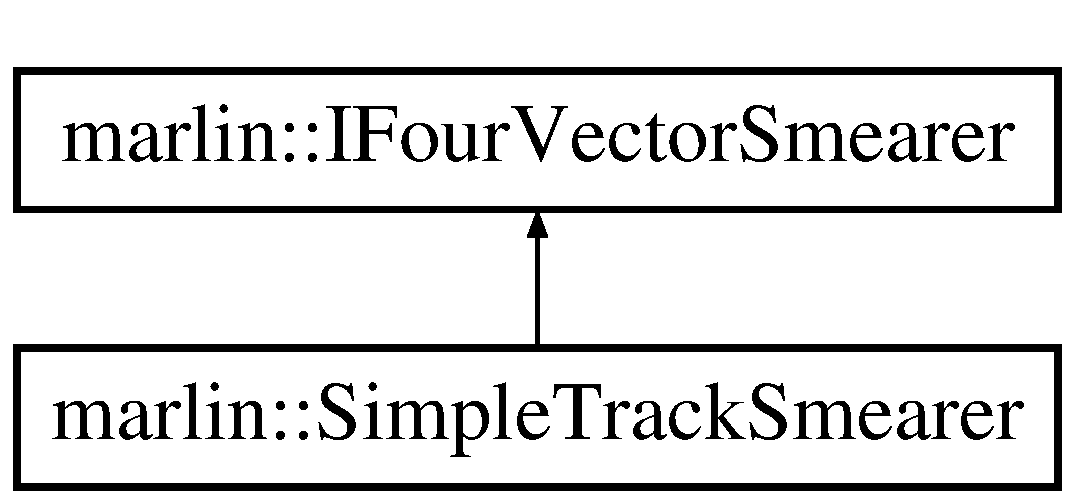
\includegraphics[height=2.000000cm]{classmarlin_1_1SimpleTrackSmearer}
\end{center}
\end{figure}
\subsection*{Public Member Functions}
\begin{DoxyCompactItemize}
\item 
\mbox{\label{classmarlin_1_1SimpleTrackSmearer_a5557fac9950d4b0c513e4a66211a4f49}} 
{\bfseries Simple\+Track\+Smearer} (const std\+::vector$<$ float $>$ \&res\+Vec)
\item 
virtual \textbf{ $\sim$\+Simple\+Track\+Smearer} ()
\begin{DoxyCompactList}\small\item\em Virtual d\textquotesingle{}tor. \end{DoxyCompactList}\item 
virtual Hep\+Lorentz\+Vector \textbf{ smeared\+Four\+Vector} (const Hep\+Lorentz\+Vector \&v, int pdg\+Code)
\begin{DoxyCompactList}\small\item\em Smears the given four vector according to the resolution for the polar angle of the track. \end{DoxyCompactList}\end{DoxyCompactItemize}
\subsection*{Protected Attributes}
\begin{DoxyCompactItemize}
\item 
\mbox{\label{classmarlin_1_1SimpleTrackSmearer_a638f0c417236014ccc38e02532a5a39d}} 
Res\+Vec {\bfseries \+\_\+res\+Vec}
\end{DoxyCompactItemize}


\subsection{Detailed Description}
Smears the four vectors of charged tracks according to d\+P/P = r for a given range of the polar angle. 

The resolutions r are given in the constructor as a vector holding triplets of\+: r0, th\+\_\+min0, th\+\_\+max0, r1, th\+\_\+min1, th\+\_\+max1, ...~\newline
 Perfect electron and muon ID is assumed to set the particle energy ( mass ) -\/ all other particles are assumed to be pions. 

\subsection{Constructor \& Destructor Documentation}
\mbox{\label{classmarlin_1_1SimpleTrackSmearer_ab0e607ceaac220f67917c8a83cf8dcc6}} 
\index{marlin\+::\+Simple\+Track\+Smearer@{marlin\+::\+Simple\+Track\+Smearer}!````~Simple\+Track\+Smearer@{$\sim$\+Simple\+Track\+Smearer}}
\index{````~Simple\+Track\+Smearer@{$\sim$\+Simple\+Track\+Smearer}!marlin\+::\+Simple\+Track\+Smearer@{marlin\+::\+Simple\+Track\+Smearer}}
\subsubsection{$\sim$\+Simple\+Track\+Smearer()}
{\footnotesize\ttfamily virtual marlin\+::\+Simple\+Track\+Smearer\+::$\sim$\+Simple\+Track\+Smearer (\begin{DoxyParamCaption}{ }\end{DoxyParamCaption})\hspace{0.3cm}{\ttfamily [inline]}, {\ttfamily [virtual]}}



Virtual d\textquotesingle{}tor. 



\subsection{Member Function Documentation}
\mbox{\label{classmarlin_1_1SimpleTrackSmearer_aa1bf44adef72e627f19dc09a9a9a838f}} 
\index{marlin\+::\+Simple\+Track\+Smearer@{marlin\+::\+Simple\+Track\+Smearer}!smeared\+Four\+Vector@{smeared\+Four\+Vector}}
\index{smeared\+Four\+Vector@{smeared\+Four\+Vector}!marlin\+::\+Simple\+Track\+Smearer@{marlin\+::\+Simple\+Track\+Smearer}}
\subsubsection{smeared\+Four\+Vector()}
{\footnotesize\ttfamily Hep\+Lorentz\+Vector marlin\+::\+Simple\+Track\+Smearer\+::smeared\+Four\+Vector (\begin{DoxyParamCaption}\item[{const Hep\+Lorentz\+Vector \&}]{v,  }\item[{int}]{pdg\+Code }\end{DoxyParamCaption})\hspace{0.3cm}{\ttfamily [virtual]}}



Smears the given four vector according to the resolution for the polar angle of the track. 

Returns a vector with all elements 0. if no resolution is defined. 

Implements \textbf{ marlin\+::\+I\+Four\+Vector\+Smearer} \doxyref{}{p.}{classmarlin_1_1IFourVectorSmearer_a69a3ece59f66350310e1eb1c696464ce}.



The documentation for this class was generated from the following files\+:\begin{DoxyCompactItemize}
\item 
Simple\+Track\+Smearer.\+h\item 
Simple\+Track\+Smearer.\+cc\end{DoxyCompactItemize}

\section{marlin\+:\+:Skip\+Event\+Exception Class Reference}
\label{classmarlin_1_1SkipEventException}\index{marlin\+::\+Skip\+Event\+Exception@{marlin\+::\+Skip\+Event\+Exception}}


\doxyref{Skip\+Event\+Exception}{p.}{classmarlin_1_1SkipEventException} used to skip the current event in \doxyref{Processor\+::process\+Event}{p.}{classmarlin_1_1Processor_a5bee49b5515f59fae755e0a26dfae91a}.  




{\ttfamily \#include $<$Exceptions.\+h$>$}

Inheritance diagram for marlin\+:\+:Skip\+Event\+Exception\+:\begin{figure}[H]
\begin{center}
\leavevmode
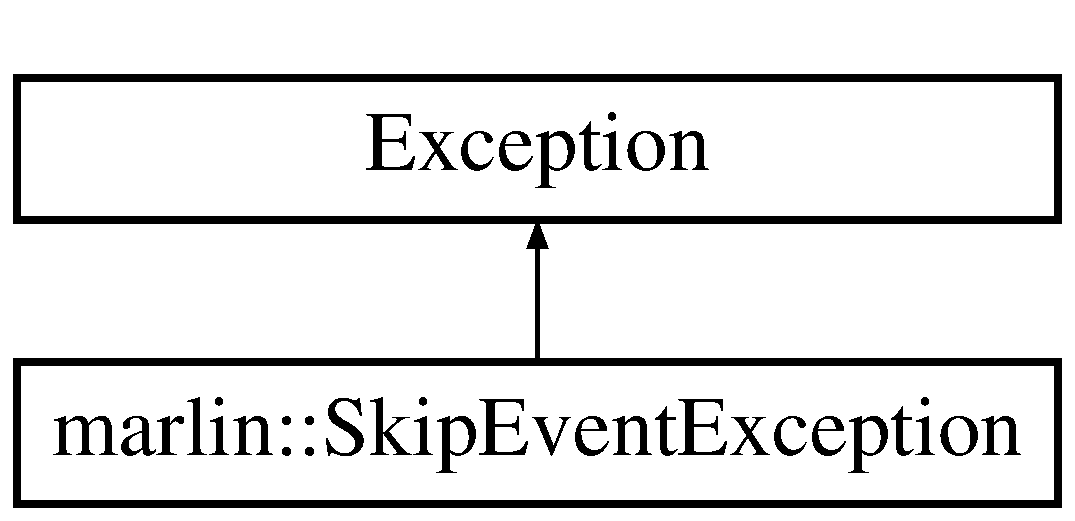
\includegraphics[height=2.000000cm]{classmarlin_1_1SkipEventException}
\end{center}
\end{figure}
\subsection*{Public Member Functions}
\begin{DoxyCompactItemize}
\item 
\mbox{\label{classmarlin_1_1SkipEventException_a33386d87a7b682db485a2b98907f0fc7}} 
{\bfseries Skip\+Event\+Exception} (const \textbf{ Processor} $\ast$proc)
\end{DoxyCompactItemize}


\subsection{Detailed Description}
\doxyref{Skip\+Event\+Exception}{p.}{classmarlin_1_1SkipEventException} used to skip the current event in \doxyref{Processor\+::process\+Event}{p.}{classmarlin_1_1Processor_a5bee49b5515f59fae755e0a26dfae91a}. 

\begin{DoxyAuthor}{Author}
gaede 
\end{DoxyAuthor}
\begin{DoxyVersion}{Version}

\end{DoxyVersion}
\begin{DoxyParagraph}{Id}
\doxyref{Exceptions.\+h}{p.}{Exceptions_8h_source},v 1.\+5 2007-\/02-\/02 17\+:15\+:25 gaede Exp 
\end{DoxyParagraph}


The documentation for this class was generated from the following files\+:\begin{DoxyCompactItemize}
\item 
Exceptions.\+h\item 
Exceptions.\+cc\end{DoxyCompactItemize}

\section{marlin\+:\+:Statusmonitor Class Reference}
\label{classmarlin_1_1Statusmonitor}\index{marlin\+::\+Statusmonitor@{marlin\+::\+Statusmonitor}}


Simple processor for writing out a status message every n-\/th event.  


Inheritance diagram for marlin\+:\+:Statusmonitor\+:\begin{figure}[H]
\begin{center}
\leavevmode
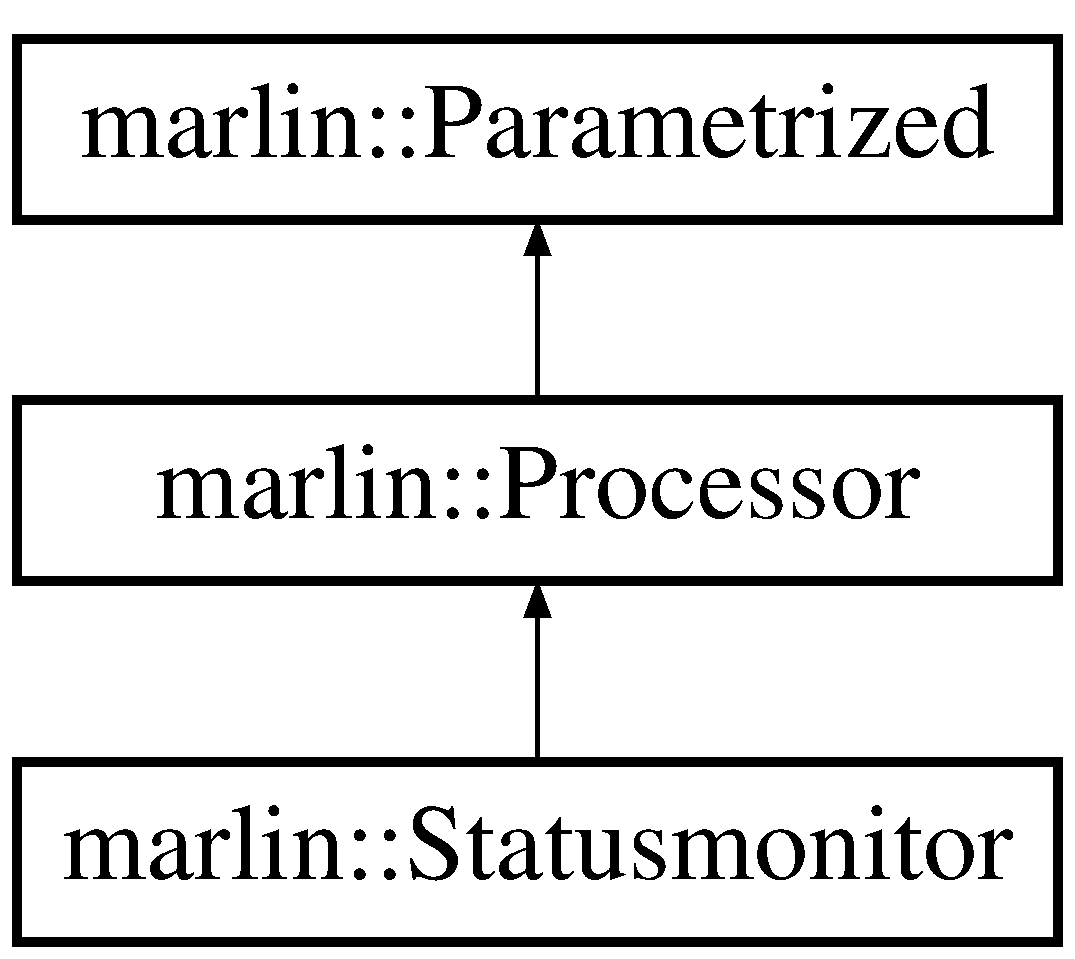
\includegraphics[height=3.000000cm]{classmarlin_1_1Statusmonitor}
\end{center}
\end{figure}
\subsection*{Public Member Functions}
\begin{DoxyCompactItemize}
\item 
\mbox{\label{classmarlin_1_1Statusmonitor_a9d655f73286217fcf0dd9fdc71f41b81}} 
\textbf{ Processor} $\ast$ \textbf{ new\+Processor} ()
\begin{DoxyCompactList}\small\item\em Return a new instance of the processor (factory method) \end{DoxyCompactList}\item 
void \textbf{ init} ()
\begin{DoxyCompactList}\small\item\em Initialize the processor. \end{DoxyCompactList}\item 
\mbox{\label{classmarlin_1_1Statusmonitor_adeab025d06acb75cb089490b8be09b3a}} 
void \textbf{ process\+Run\+Header} (E\+V\+E\+N\+T\+::\+L\+C\+Run\+Header $\ast$run)
\begin{DoxyCompactList}\small\item\em Called for every run. \end{DoxyCompactList}\item 
\mbox{\label{classmarlin_1_1Statusmonitor_a845784ae1226f43f2d4db27ee6d261cf}} 
void \textbf{ process\+Event} (E\+V\+E\+N\+T\+::\+L\+C\+Event $\ast$evt)
\begin{DoxyCompactList}\small\item\em Called for every event -\/ the working horse. \end{DoxyCompactList}\item 
\mbox{\label{classmarlin_1_1Statusmonitor_ac431675646f711f978a0f1ca2faf9e02}} 
void \textbf{ end} ()
\begin{DoxyCompactList}\small\item\em Called after data processing for clean up. \end{DoxyCompactList}\end{DoxyCompactItemize}
\subsection*{Additional Inherited Members}


\subsection{Detailed Description}
Simple processor for writing out a status message every n-\/th event. 

\subparagraph*{Input -\/ Prerequisites}

none \subparagraph*{Output}

none  How\+Often print run and event number for every How\+Often-\/th event

\begin{DoxyAuthor}{Author}
A.\+Sailer C\+E\+RN 
\end{DoxyAuthor}
\begin{DoxyVersion}{Version}
\$\+Id\+:\$ 
\end{DoxyVersion}


\subsection{Member Function Documentation}
\mbox{\label{classmarlin_1_1Statusmonitor_a2a01fb3ca1afe2677efad92aa9bb48c5}} 
\index{marlin\+::\+Statusmonitor@{marlin\+::\+Statusmonitor}!init@{init}}
\index{init@{init}!marlin\+::\+Statusmonitor@{marlin\+::\+Statusmonitor}}
\subsubsection{init()}
{\footnotesize\ttfamily void marlin\+::\+Statusmonitor\+::init (\begin{DoxyParamCaption}{ }\end{DoxyParamCaption})\hspace{0.3cm}{\ttfamily [virtual]}}



Initialize the processor. 

Called at the begin of the job before anything is read. Use to initialize the processor, e.\+g. book histograms. 

Reimplemented from \textbf{ marlin\+::\+Processor} \doxyref{}{p.}{classmarlin_1_1Processor_a8194fb92a428de40ea9d891c8c8aed6b}.



References marlin\+::\+Processor\+::print\+Parameters().



Referenced by new\+Processor().



The documentation for this class was generated from the following file\+:\begin{DoxyCompactItemize}
\item 
Statusmonitor.\+cc\end{DoxyCompactItemize}

\section{marlin\+:\+:Std\+Hep\+File\+Source Class Reference}
\label{classmarlin_1_1StdHepFileSource}\index{marlin\+::\+Std\+Hep\+File\+Source@{marlin\+::\+Std\+Hep\+File\+Source}}


\doxyref{Std\+Hep\+File\+Source}{p.}{classmarlin_1_1StdHepFileSource} class.  


Inheritance diagram for marlin\+:\+:Std\+Hep\+File\+Source\+:\begin{figure}[H]
\begin{center}
\leavevmode
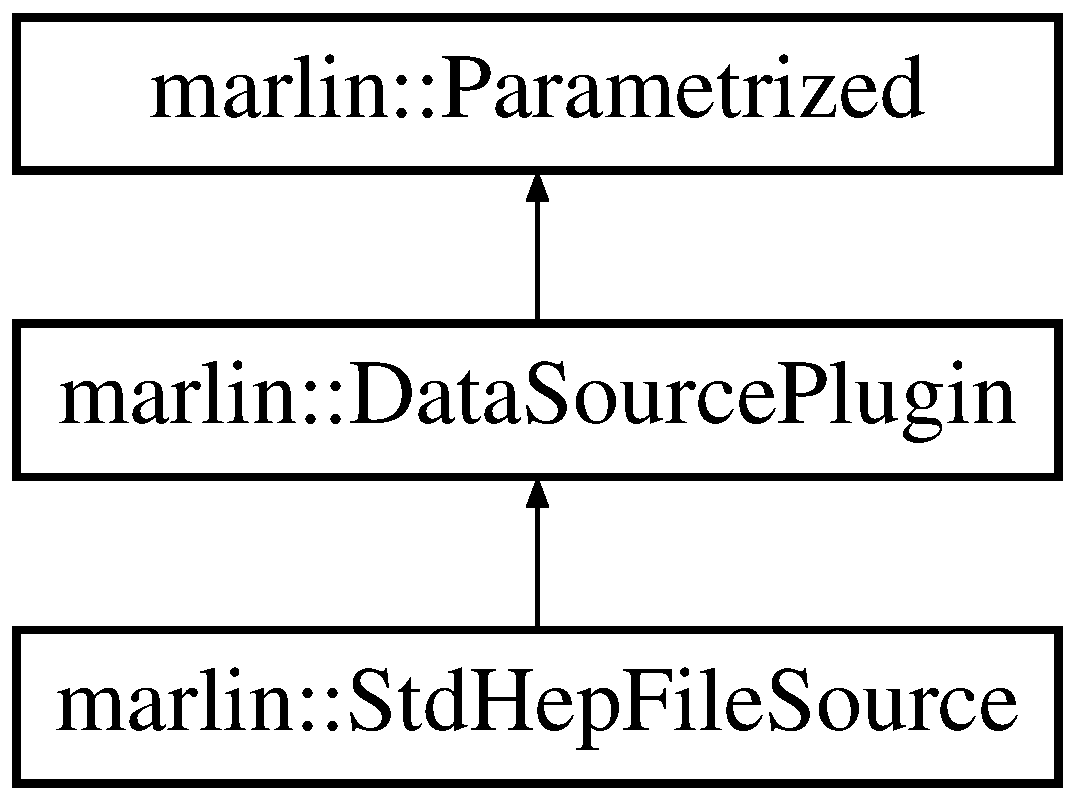
\includegraphics[height=3.000000cm]{classmarlin_1_1StdHepFileSource}
\end{center}
\end{figure}
\subsection*{Public Member Functions}
\begin{DoxyCompactItemize}
\item 
\mbox{\label{classmarlin_1_1StdHepFileSource_a88f746f2906ba152b2300ea30285c144}} 
void \textbf{ init} ()
\begin{DoxyCompactList}\small\item\em Initialize the plugin. \end{DoxyCompactList}\item 
bool \textbf{ read\+One} ()
\begin{DoxyCompactList}\small\item\em Read one record from the input stream. \end{DoxyCompactList}\end{DoxyCompactItemize}
\subsection*{Additional Inherited Members}


\subsection{Detailed Description}
\doxyref{Std\+Hep\+File\+Source}{p.}{classmarlin_1_1StdHepFileSource} class. 

\subsection{Member Function Documentation}
\mbox{\label{classmarlin_1_1StdHepFileSource_a0dc43528a14d38dc6277ba300f5fecb8}} 
\index{marlin\+::\+Std\+Hep\+File\+Source@{marlin\+::\+Std\+Hep\+File\+Source}!read\+One@{read\+One}}
\index{read\+One@{read\+One}!marlin\+::\+Std\+Hep\+File\+Source@{marlin\+::\+Std\+Hep\+File\+Source}}
\subsubsection{read\+One()}
{\footnotesize\ttfamily bool marlin\+::\+Std\+Hep\+File\+Source\+::read\+One (\begin{DoxyParamCaption}{ }\end{DoxyParamCaption})\hspace{0.3cm}{\ttfamily [virtual]}}



Read one record from the input stream. 

Users must call \doxyref{process\+Run\+Header()}{p.}{classmarlin_1_1DataSourcePlugin_a769e257658ee89c176857191773c26b3} or \doxyref{process\+Event()}{p.}{classmarlin_1_1DataSourcePlugin_add4afa8b047d3a2e4e33a9957e75d9bb} to forward it to the framework. Returns true on success. If the end of the stream is reached, return false. 

Implements \textbf{ marlin\+::\+Data\+Source\+Plugin} \doxyref{}{p.}{classmarlin_1_1DataSourcePlugin_a9e174b63facdc108425e79fca9022404}.



The documentation for this class was generated from the following file\+:\begin{DoxyCompactItemize}
\item 
Std\+Hep\+File\+Source.\+cc\end{DoxyCompactItemize}

\section{marlin\+:\+:Stop\+Processing\+Exception Class Reference}
\label{classmarlin_1_1StopProcessingException}\index{marlin\+::\+Stop\+Processing\+Exception@{marlin\+::\+Stop\+Processing\+Exception}}


\doxyref{Stop\+Processing\+Exception}{p.}{classmarlin_1_1StopProcessingException} used to stop the current proccessing of events and call \doxyref{Processor\+::end()}{p.}{classmarlin_1_1Processor_a40c4bc6d5b67906954392c5bb1df28c1}.  




{\ttfamily \#include $<$Exceptions.\+h$>$}

Inheritance diagram for marlin\+:\+:Stop\+Processing\+Exception\+:\begin{figure}[H]
\begin{center}
\leavevmode
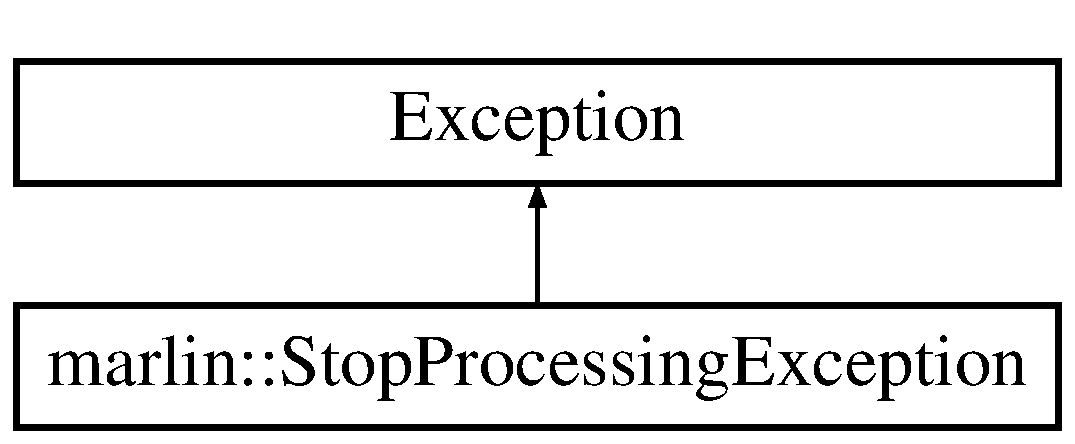
\includegraphics[height=2.000000cm]{classmarlin_1_1StopProcessingException}
\end{center}
\end{figure}
\subsection*{Public Member Functions}
\begin{DoxyCompactItemize}
\item 
\mbox{\label{classmarlin_1_1StopProcessingException_a1ca7b91dfb9e4f4e7e31d9f3e40674b8}} 
{\bfseries Stop\+Processing\+Exception} (const \textbf{ Processor} $\ast$proc)
\end{DoxyCompactItemize}


\subsection{Detailed Description}
\doxyref{Stop\+Processing\+Exception}{p.}{classmarlin_1_1StopProcessingException} used to stop the current proccessing of events and call \doxyref{Processor\+::end()}{p.}{classmarlin_1_1Processor_a40c4bc6d5b67906954392c5bb1df28c1}. 

\begin{DoxyAuthor}{Author}
gaede 
\end{DoxyAuthor}
\begin{DoxyVersion}{Version}

\end{DoxyVersion}
\begin{DoxyParagraph}{Id}
\doxyref{Exceptions.\+h}{p.}{Exceptions_8h_source},v 1.\+5 2007-\/02-\/02 17\+:15\+:25 gaede Exp 
\end{DoxyParagraph}


The documentation for this class was generated from the following files\+:\begin{DoxyCompactItemize}
\item 
Exceptions.\+h\item 
Exceptions.\+cc\end{DoxyCompactItemize}

\section{marlin\+:\+:String\+Parameters Class Reference}
\label{classmarlin_1_1StringParameters}\index{marlin\+::\+String\+Parameters@{marlin\+::\+String\+Parameters}}


Simple parameters class for Marlin.  




{\ttfamily \#include $<$String\+Parameters.\+h$>$}

\subsection*{Public Member Functions}
\begin{DoxyCompactItemize}
\item 
\mbox{\label{classmarlin_1_1StringParameters_ac77daec7e6d882404fa588671e445944}} 
{\bfseries String\+Parameters} (const \textbf{ String\+Parameters} \&sp)=default
\item 
void \textbf{ add} (const std\+::string \&key)
\begin{DoxyCompactList}\small\item\em Add a parameter without value. \end{DoxyCompactList}\item 
{\footnotesize template$<$typename T $>$ }\\void \textbf{ add} (const std\+::string \&key, const T \&value)
\begin{DoxyCompactList}\small\item\em Add a parameter with its value. \end{DoxyCompactList}\item 
{\footnotesize template$<$typename T $>$ }\\void \textbf{ add} (const std\+::string \&key, const std\+::vector$<$ T $>$ \&values)
\begin{DoxyCompactList}\small\item\em Add a parameter with its values. \end{DoxyCompactList}\item 
{\footnotesize template$<$typename T $>$ }\\void \textbf{ replace} (const std\+::string \&key, const T \&value)
\begin{DoxyCompactList}\small\item\em Replace a parameter with a new value. \end{DoxyCompactList}\item 
{\footnotesize template$<$typename T $>$ }\\void \textbf{ replace} (const std\+::string \&key, const std\+::vector$<$ T $>$ \&values)
\begin{DoxyCompactList}\small\item\em Replace a parameter with a new values. \end{DoxyCompactList}\item 
void \textbf{ erase} (const std\+::string \&key)
\begin{DoxyCompactList}\small\item\em Erase a parameter. \end{DoxyCompactList}\item 
bool \textbf{ is\+Parameter\+Set} (const std\+::string \&key) const
\begin{DoxyCompactList}\small\item\em Whether the parameter is set, meaning the entry already exists, but has no value. \end{DoxyCompactList}\item 
bool \textbf{ exists} (const std\+::string \&key) const
\begin{DoxyCompactList}\small\item\em Whether the parameter exists. \end{DoxyCompactList}\item 
void \textbf{ unset} (const std\+::string \&key)
\begin{DoxyCompactList}\small\item\em Unset a parameter. \end{DoxyCompactList}\item 
\mbox{\label{classmarlin_1_1StringParameters_af3b142c6b4ddc37e64ed3b8f2af0f287}} 
void \textbf{ unset} ()
\begin{DoxyCompactList}\small\item\em Unset all parameters. \end{DoxyCompactList}\item 
\mbox{\label{classmarlin_1_1StringParameters_aacaa6d24f3012a5bb74679608b3975df}} 
std\+::vector$<$ std\+::string $>$ \textbf{ keys} () const
\begin{DoxyCompactList}\small\item\em Get the parameter keys. \end{DoxyCompactList}\item 
{\footnotesize template$<$typename T $>$ }\\T \textbf{ get\+Value} (const std\+::string \&key) const
\begin{DoxyCompactList}\small\item\em Get a parameter value. \end{DoxyCompactList}\item 
{\footnotesize template$<$typename T $>$ }\\std\+::vector$<$ T $>$ \textbf{ get\+Values} (const std\+::string \&key) const
\begin{DoxyCompactList}\small\item\em Get parameter values. \end{DoxyCompactList}\item 
{\footnotesize template$<$typename T $>$ }\\T \textbf{ get\+Value} (const std\+::string \&key, const T \&fallback) const
\begin{DoxyCompactList}\small\item\em Get a parameter value. \end{DoxyCompactList}\item 
{\footnotesize template$<$typename T $>$ }\\std\+::vector$<$ T $>$ \textbf{ get\+Values} (const std\+::string \&key, const std\+::vector$<$ T $>$ \&fallback) const
\begin{DoxyCompactList}\small\item\em Get parameter values. \end{DoxyCompactList}\item 
{\footnotesize template$<$typename T $>$ }\\void \textbf{ get} (const std\+::string \&key, T \&value) const
\begin{DoxyCompactList}\small\item\em Get a parameter value by reference. \end{DoxyCompactList}\item 
{\footnotesize template$<$typename T $>$ }\\void \textbf{ get} (const std\+::string \&key, std\+::vector$<$ T $>$ \&values) const
\begin{DoxyCompactList}\small\item\em Get parameter values by reference. \end{DoxyCompactList}\end{DoxyCompactItemize}
\subsection*{Protected Attributes}
\begin{DoxyCompactItemize}
\item 
\mbox{\label{classmarlin_1_1StringParameters_a57b12116d1220edd90ddfb5a85f6e88b}} 
Parameters\+Map \textbf{ \+\_\+map} \{\}
\begin{DoxyCompactList}\small\item\em $<$ The parameters map \end{DoxyCompactList}\end{DoxyCompactItemize}
\subsection*{Friends}
\begin{DoxyCompactItemize}
\item 
\mbox{\label{classmarlin_1_1StringParameters_a8ea205e1f0462cefd77c51231b34917f}} 
std\+::ostream \& {\bfseries operator$<$$<$} (std\+::ostream \&, const \textbf{ String\+Parameters} \&)
\end{DoxyCompactItemize}


\subsection{Detailed Description}
Simple parameters class for Marlin. 

Holds named parameters as string vectors. \begin{DoxyAuthor}{Author}
F. Gaede, D\+E\+SY 

R. Ete, D\+E\+SY 
\end{DoxyAuthor}
\begin{DoxyVersion}{Version}

\end{DoxyVersion}
\begin{DoxyParagraph}{Id}
\doxyref{String\+Parameters.\+h}{p.}{StringParameters_8h_source},v 1.\+5 2006-\/11-\/10 11\+:56\+:07 engels Exp 
\end{DoxyParagraph}


\subsection{Member Function Documentation}
\mbox{\label{classmarlin_1_1StringParameters_a66e54faeeb784b5f06c8f5dc4f0dc5cf}} 
\index{marlin\+::\+String\+Parameters@{marlin\+::\+String\+Parameters}!add@{add}}
\index{add@{add}!marlin\+::\+String\+Parameters@{marlin\+::\+String\+Parameters}}
\subsubsection{add()\hspace{0.1cm}{\footnotesize\ttfamily [1/3]}}
{\footnotesize\ttfamily void marlin\+::\+String\+Parameters\+::add (\begin{DoxyParamCaption}\item[{const std\+::string \&}]{key }\end{DoxyParamCaption})}



Add a parameter without value. 

Does nothing if the parameter exists


\begin{DoxyParams}{Parameters}
{\em key} & the prameter key \\
\hline
\end{DoxyParams}


References \+\_\+map.



Referenced by add(), marlin\+::\+Parser\+::parse(), and replace().

\mbox{\label{classmarlin_1_1StringParameters_a83f7c882fd90473619169f3d4cbe2c30}} 
\index{marlin\+::\+String\+Parameters@{marlin\+::\+String\+Parameters}!add@{add}}
\index{add@{add}!marlin\+::\+String\+Parameters@{marlin\+::\+String\+Parameters}}
\subsubsection{add()\hspace{0.1cm}{\footnotesize\ttfamily [2/3]}}
{\footnotesize\ttfamily template$<$typename T $>$ \\
void marlin\+::\+String\+Parameters\+::add (\begin{DoxyParamCaption}\item[{const std\+::string \&}]{key,  }\item[{const T \&}]{value }\end{DoxyParamCaption})\hspace{0.3cm}{\ttfamily [inline]}}



Add a parameter with its value. 

Note that the value is appended to the parameter list. To overwrite a parameter value, use \doxyref{replace()}{p.}{classmarlin_1_1StringParameters_afa4a13eccfd8692f01423d22beb6c28b} instead


\begin{DoxyParams}{Parameters}
{\em key} & the parameter key \\
\hline
{\em value} & the parameter value \\
\hline
\end{DoxyParams}


References \+\_\+map, and add().

\mbox{\label{classmarlin_1_1StringParameters_a17aac2fa25b6d675843a5615ea25f0d6}} 
\index{marlin\+::\+String\+Parameters@{marlin\+::\+String\+Parameters}!add@{add}}
\index{add@{add}!marlin\+::\+String\+Parameters@{marlin\+::\+String\+Parameters}}
\subsubsection{add()\hspace{0.1cm}{\footnotesize\ttfamily [3/3]}}
{\footnotesize\ttfamily template$<$typename T $>$ \\
void marlin\+::\+String\+Parameters\+::add (\begin{DoxyParamCaption}\item[{const std\+::string \&}]{key,  }\item[{const std\+::vector$<$ T $>$ \&}]{values }\end{DoxyParamCaption})\hspace{0.3cm}{\ttfamily [inline]}}



Add a parameter with its values. 

Note that the values are appended to the parameter list. To overwrite a parameter value, use \doxyref{replace()}{p.}{classmarlin_1_1StringParameters_afa4a13eccfd8692f01423d22beb6c28b} instead


\begin{DoxyParams}{Parameters}
{\em key} & the parameter key \\
\hline
{\em values} & the parameter values \\
\hline
\end{DoxyParams}


References \+\_\+map, and add().

\mbox{\label{classmarlin_1_1StringParameters_a4b2bac2a57934a1c85c0327a011f9b0e}} 
\index{marlin\+::\+String\+Parameters@{marlin\+::\+String\+Parameters}!erase@{erase}}
\index{erase@{erase}!marlin\+::\+String\+Parameters@{marlin\+::\+String\+Parameters}}
\subsubsection{erase()}
{\footnotesize\ttfamily void marlin\+::\+String\+Parameters\+::erase (\begin{DoxyParamCaption}\item[{const std\+::string \&}]{key }\end{DoxyParamCaption})}



Erase a parameter. 


\begin{DoxyParams}{Parameters}
{\em key} & the parameter key \\
\hline
\end{DoxyParams}


References \+\_\+map.



Referenced by replace().

\mbox{\label{classmarlin_1_1StringParameters_a3193ba4d1d33d7417823261b88340bfc}} 
\index{marlin\+::\+String\+Parameters@{marlin\+::\+String\+Parameters}!exists@{exists}}
\index{exists@{exists}!marlin\+::\+String\+Parameters@{marlin\+::\+String\+Parameters}}
\subsubsection{exists()}
{\footnotesize\ttfamily bool marlin\+::\+String\+Parameters\+::exists (\begin{DoxyParamCaption}\item[{const std\+::string \&}]{key }\end{DoxyParamCaption}) const}



Whether the parameter exists. 


\begin{DoxyParams}{Parameters}
{\em key} & the parameter key \\
\hline
\end{DoxyParams}


References \+\_\+map.

\mbox{\label{classmarlin_1_1StringParameters_aac2a0dfcfdc004fa4f3e07f38d7d9cf9}} 
\index{marlin\+::\+String\+Parameters@{marlin\+::\+String\+Parameters}!get@{get}}
\index{get@{get}!marlin\+::\+String\+Parameters@{marlin\+::\+String\+Parameters}}
\subsubsection{get()\hspace{0.1cm}{\footnotesize\ttfamily [1/2]}}
{\footnotesize\ttfamily template$<$typename T $>$ \\
void marlin\+::\+String\+Parameters\+::get (\begin{DoxyParamCaption}\item[{const std\+::string \&}]{key,  }\item[{T \&}]{value }\end{DoxyParamCaption}) const\hspace{0.3cm}{\ttfamily [inline]}}



Get a parameter value by reference. 


\begin{DoxyParams}{Parameters}
{\em key} & the parameter key \\
\hline
{\em value} & the value to receive \\
\hline
\end{DoxyParams}


References \+\_\+map.



Referenced by marlin\+::\+Parser\+::parse(), marlin\+::\+X\+M\+L\+Parser\+::parse(), and marlin\+::\+Parameter\+T$<$ T $>$\+::set\+Value().

\mbox{\label{classmarlin_1_1StringParameters_a322143c457d87d615f73346ce051e0d8}} 
\index{marlin\+::\+String\+Parameters@{marlin\+::\+String\+Parameters}!get@{get}}
\index{get@{get}!marlin\+::\+String\+Parameters@{marlin\+::\+String\+Parameters}}
\subsubsection{get()\hspace{0.1cm}{\footnotesize\ttfamily [2/2]}}
{\footnotesize\ttfamily template$<$typename T $>$ \\
void marlin\+::\+String\+Parameters\+::get (\begin{DoxyParamCaption}\item[{const std\+::string \&}]{key,  }\item[{std\+::vector$<$ T $>$ \&}]{values }\end{DoxyParamCaption}) const\hspace{0.3cm}{\ttfamily [inline]}}



Get parameter values by reference. 


\begin{DoxyParams}{Parameters}
{\em key} & the parameter key \\
\hline
{\em values} & the values to receive \\
\hline
\end{DoxyParams}


References \+\_\+map.

\mbox{\label{classmarlin_1_1StringParameters_a8aa058fc6d4969250e7497826accfab4}} 
\index{marlin\+::\+String\+Parameters@{marlin\+::\+String\+Parameters}!get\+Value@{get\+Value}}
\index{get\+Value@{get\+Value}!marlin\+::\+String\+Parameters@{marlin\+::\+String\+Parameters}}
\subsubsection{get\+Value()\hspace{0.1cm}{\footnotesize\ttfamily [1/2]}}
{\footnotesize\ttfamily template$<$typename T $>$ \\
T marlin\+::\+String\+Parameters\+::get\+Value (\begin{DoxyParamCaption}\item[{const std\+::string \&}]{key }\end{DoxyParamCaption}) const\hspace{0.3cm}{\ttfamily [inline]}}



Get a parameter value. 

If the value doesn\textquotesingle{}t exists, an exception is thrown.


\begin{DoxyParams}{Parameters}
{\em key} & the parameter key \\
\hline
\end{DoxyParams}


References \+\_\+map.



Referenced by marlin\+::\+Parser\+::parse().

\mbox{\label{classmarlin_1_1StringParameters_a1600af85fd6b79de266ad96698647c64}} 
\index{marlin\+::\+String\+Parameters@{marlin\+::\+String\+Parameters}!get\+Value@{get\+Value}}
\index{get\+Value@{get\+Value}!marlin\+::\+String\+Parameters@{marlin\+::\+String\+Parameters}}
\subsubsection{get\+Value()\hspace{0.1cm}{\footnotesize\ttfamily [2/2]}}
{\footnotesize\ttfamily template$<$typename T $>$ \\
T marlin\+::\+String\+Parameters\+::get\+Value (\begin{DoxyParamCaption}\item[{const std\+::string \&}]{key,  }\item[{const T \&}]{fallback }\end{DoxyParamCaption}) const\hspace{0.3cm}{\ttfamily [inline]}}



Get a parameter value. 

If the value doesn\textquotesingle{}t exists, the fallback value provided as second argument is returned


\begin{DoxyParams}{Parameters}
{\em key} & the parameter key \\
\hline
{\em fallback} & the fallback value if not found \\
\hline
\end{DoxyParams}


References \+\_\+map.

\mbox{\label{classmarlin_1_1StringParameters_a483014ccaadc2ad38f5cf03ad15a591c}} 
\index{marlin\+::\+String\+Parameters@{marlin\+::\+String\+Parameters}!get\+Values@{get\+Values}}
\index{get\+Values@{get\+Values}!marlin\+::\+String\+Parameters@{marlin\+::\+String\+Parameters}}
\subsubsection{get\+Values()\hspace{0.1cm}{\footnotesize\ttfamily [1/2]}}
{\footnotesize\ttfamily template$<$typename T $>$ \\
std\+::vector$<$ T $>$ marlin\+::\+String\+Parameters\+::get\+Values (\begin{DoxyParamCaption}\item[{const std\+::string \&}]{key }\end{DoxyParamCaption}) const\hspace{0.3cm}{\ttfamily [inline]}}



Get parameter values. 

If the values do not exists, an exception is thrown.


\begin{DoxyParams}{Parameters}
{\em key} & the parameter key \\
\hline
\end{DoxyParams}


References \+\_\+map.

\mbox{\label{classmarlin_1_1StringParameters_a22034f768bc5a208f33799fe1b536671}} 
\index{marlin\+::\+String\+Parameters@{marlin\+::\+String\+Parameters}!get\+Values@{get\+Values}}
\index{get\+Values@{get\+Values}!marlin\+::\+String\+Parameters@{marlin\+::\+String\+Parameters}}
\subsubsection{get\+Values()\hspace{0.1cm}{\footnotesize\ttfamily [2/2]}}
{\footnotesize\ttfamily template$<$typename T $>$ \\
std\+::vector$<$ T $>$ marlin\+::\+String\+Parameters\+::get\+Values (\begin{DoxyParamCaption}\item[{const std\+::string \&}]{key,  }\item[{const std\+::vector$<$ T $>$ \&}]{fallback }\end{DoxyParamCaption}) const\hspace{0.3cm}{\ttfamily [inline]}}



Get parameter values. 

If the values do not exists, the fallback values provided as second argument is returned


\begin{DoxyParams}{Parameters}
{\em key} & the parameter key \\
\hline
{\em fallback} & the fallback value if not found \\
\hline
\end{DoxyParams}


References \+\_\+map.

\mbox{\label{classmarlin_1_1StringParameters_a51f2fde182c52d292766b5d3029c7a5f}} 
\index{marlin\+::\+String\+Parameters@{marlin\+::\+String\+Parameters}!is\+Parameter\+Set@{is\+Parameter\+Set}}
\index{is\+Parameter\+Set@{is\+Parameter\+Set}!marlin\+::\+String\+Parameters@{marlin\+::\+String\+Parameters}}
\subsubsection{is\+Parameter\+Set()}
{\footnotesize\ttfamily bool marlin\+::\+String\+Parameters\+::is\+Parameter\+Set (\begin{DoxyParamCaption}\item[{const std\+::string \&}]{key }\end{DoxyParamCaption}) const}



Whether the parameter is set, meaning the entry already exists, but has no value. 

To check if a parameter exists, use \doxyref{exists()}{p.}{classmarlin_1_1StringParameters_a3193ba4d1d33d7417823261b88340bfc} instead


\begin{DoxyParams}{Parameters}
{\em key} & the parameter key \\
\hline
\end{DoxyParams}


References \+\_\+map.



Referenced by marlin\+::\+Parameter\+T$<$ T $>$\+::set\+Value().

\mbox{\label{classmarlin_1_1StringParameters_afa4a13eccfd8692f01423d22beb6c28b}} 
\index{marlin\+::\+String\+Parameters@{marlin\+::\+String\+Parameters}!replace@{replace}}
\index{replace@{replace}!marlin\+::\+String\+Parameters@{marlin\+::\+String\+Parameters}}
\subsubsection{replace()\hspace{0.1cm}{\footnotesize\ttfamily [1/2]}}
{\footnotesize\ttfamily template$<$typename T $>$ \\
void marlin\+::\+String\+Parameters\+::replace (\begin{DoxyParamCaption}\item[{const std\+::string \&}]{key,  }\item[{const T \&}]{value }\end{DoxyParamCaption})\hspace{0.3cm}{\ttfamily [inline]}}



Replace a parameter with a new value. 


\begin{DoxyParams}{Parameters}
{\em key} & the parameter key \\
\hline
{\em value} & the parameter value \\
\hline
\end{DoxyParams}


References add(), and erase().

\mbox{\label{classmarlin_1_1StringParameters_a2da733d0f5f9e5ff5a626d9f7dbe7763}} 
\index{marlin\+::\+String\+Parameters@{marlin\+::\+String\+Parameters}!replace@{replace}}
\index{replace@{replace}!marlin\+::\+String\+Parameters@{marlin\+::\+String\+Parameters}}
\subsubsection{replace()\hspace{0.1cm}{\footnotesize\ttfamily [2/2]}}
{\footnotesize\ttfamily template$<$typename T $>$ \\
void marlin\+::\+String\+Parameters\+::replace (\begin{DoxyParamCaption}\item[{const std\+::string \&}]{key,  }\item[{const std\+::vector$<$ T $>$ \&}]{values }\end{DoxyParamCaption})\hspace{0.3cm}{\ttfamily [inline]}}



Replace a parameter with a new values. 


\begin{DoxyParams}{Parameters}
{\em key} & the parameter key \\
\hline
{\em values} & the parameter values \\
\hline
\end{DoxyParams}


References add(), and erase().

\mbox{\label{classmarlin_1_1StringParameters_ab23f013a75f38607b718246d45dc207f}} 
\index{marlin\+::\+String\+Parameters@{marlin\+::\+String\+Parameters}!unset@{unset}}
\index{unset@{unset}!marlin\+::\+String\+Parameters@{marlin\+::\+String\+Parameters}}
\subsubsection{unset()}
{\footnotesize\ttfamily void marlin\+::\+String\+Parameters\+::unset (\begin{DoxyParamCaption}\item[{const std\+::string \&}]{key }\end{DoxyParamCaption})}



Unset a parameter. 


\begin{DoxyParams}{Parameters}
{\em key} & the parameter key \\
\hline
\end{DoxyParams}


References \+\_\+map.



The documentation for this class was generated from the following files\+:\begin{DoxyCompactItemize}
\item 
String\+Parameters.\+h\item 
String\+Parameters.\+cc\end{DoxyCompactItemize}

\section{marlin\+:\+:String\+Util Class Reference}
\label{classmarlin_1_1StringUtil}\index{marlin\+::\+String\+Util@{marlin\+::\+String\+Util}}


\doxyref{String\+Util}{p.}{classmarlin_1_1StringUtil} class Simple utility class for string operations.  




{\ttfamily \#include $<$Utils.\+h$>$}

\subsection*{Public Member Functions}
\begin{DoxyCompactItemize}
\item 
\mbox{\label{classmarlin_1_1StringUtil_ab2c564055c2db79c1435a4c9dc53c096}} 
{\footnotesize template$<$$>$ }\\std\+::string {\bfseries type\+To\+String} (const std\+::string \&var)
\item 
\mbox{\label{classmarlin_1_1StringUtil_a093fa7e9e8475f70438ed5ff372e8a2a}} 
{\footnotesize template$<$$>$ }\\std\+::string {\bfseries type\+To\+String} (const bool \&var)
\item 
\mbox{\label{classmarlin_1_1StringUtil_a2a923b0d7048ee72df8b911c8823b6d1}} 
{\footnotesize template$<$$>$ }\\std\+::string {\bfseries string\+To\+Type} (const std\+::string \&str)
\item 
\mbox{\label{classmarlin_1_1StringUtil_a38e3e0ccc8ea41e8da3b207b41167adf}} 
{\footnotesize template$<$$>$ }\\bool {\bfseries string\+To\+Type} (const std\+::string \&str)
\end{DoxyCompactItemize}
\subsection*{Static Public Member Functions}
\begin{DoxyCompactItemize}
\item 
{\footnotesize template$<$typename T $>$ }\\static std\+::string \textbf{ type\+To\+String} (const T \&var)
\begin{DoxyCompactList}\small\item\em Convert a type to string. \end{DoxyCompactList}\item 
{\footnotesize template$<$typename T $>$ }\\static std\+::vector$<$ std\+::string $>$ \textbf{ type\+To\+String} (const std\+::vector$<$ T $>$ \&vars)
\begin{DoxyCompactList}\small\item\em Convert a vector of type to vector of string. \end{DoxyCompactList}\item 
{\footnotesize template$<$typename T $>$ }\\static T \textbf{ string\+To\+Type} (const std\+::string \&str)
\begin{DoxyCompactList}\small\item\em Convert a variable to string. \end{DoxyCompactList}\item 
{\footnotesize template$<$typename T $>$ }\\static std\+::vector$<$ T $>$ \textbf{ string\+To\+Type} (const std\+::vector$<$ std\+::string $>$ \&strs)
\begin{DoxyCompactList}\small\item\em Convert a string vector to a vector of specified type. \end{DoxyCompactList}\item 
{\footnotesize template$<$typename T $>$ }\\static std\+::vector$<$ T $>$ \textbf{ split} (const std\+::string \&input\+String, const std\+::string \&delimiter=\char`\"{} \char`\"{})
\begin{DoxyCompactList}\small\item\em Split the string with the corresponding delimiter. \end{DoxyCompactList}\item 
{\footnotesize template$<$typename T $>$ }\\static std\+::string \textbf{ join} (const T \&input, const std\+::string \&delimiter=\char`\"{} \char`\"{})
\begin{DoxyCompactList}\small\item\em Weird overload for scalar types. \end{DoxyCompactList}\item 
{\footnotesize template$<$typename T $>$ }\\static std\+::string \textbf{ join} (const std\+::vector$<$ T $>$ \&input, const std\+::string \&delimiter=\char`\"{} \char`\"{})
\begin{DoxyCompactList}\small\item\em Join the input values from the vector with the corresponding delimiter and returns a string representation of it. \end{DoxyCompactList}\end{DoxyCompactItemize}


\subsection{Detailed Description}
\doxyref{String\+Util}{p.}{classmarlin_1_1StringUtil} class Simple utility class for string operations. 

\subsection{Member Function Documentation}
\mbox{\label{classmarlin_1_1StringUtil_a15a81255e9cd2ca50b35ba370e78b320}} 
\index{marlin\+::\+String\+Util@{marlin\+::\+String\+Util}!join@{join}}
\index{join@{join}!marlin\+::\+String\+Util@{marlin\+::\+String\+Util}}
\subsubsection{join()\hspace{0.1cm}{\footnotesize\ttfamily [1/2]}}
{\footnotesize\ttfamily template$<$typename T $>$ \\
std\+::string marlin\+::\+String\+Util\+::join (\begin{DoxyParamCaption}\item[{const T \&}]{input,  }\item[{const std\+::string \&}]{delimiter = {\ttfamily \char`\"{}~\char`\"{}} }\end{DoxyParamCaption})\hspace{0.3cm}{\ttfamily [inline]}, {\ttfamily [static]}}



Weird overload for scalar types. 

Just returns the conversion to string. See overload version with vector instead.


\begin{DoxyParams}{Parameters}
{\em input} & the input value \\
\hline
{\em delimiter} & the string delimiter (unused here) \\
\hline
\end{DoxyParams}


Referenced by marlin\+::\+Parameter\+T$<$ T $>$\+::default\+Value(), and marlin\+::\+Parameter\+T$<$ T $>$\+::value().

\mbox{\label{classmarlin_1_1StringUtil_acf6313cb4a8057b3c0c2aea4b97378d2}} 
\index{marlin\+::\+String\+Util@{marlin\+::\+String\+Util}!join@{join}}
\index{join@{join}!marlin\+::\+String\+Util@{marlin\+::\+String\+Util}}
\subsubsection{join()\hspace{0.1cm}{\footnotesize\ttfamily [2/2]}}
{\footnotesize\ttfamily template$<$typename T $>$ \\
std\+::string marlin\+::\+String\+Util\+::join (\begin{DoxyParamCaption}\item[{const std\+::vector$<$ T $>$ \&}]{input,  }\item[{const std\+::string \&}]{delimiter = {\ttfamily \char`\"{}~\char`\"{}} }\end{DoxyParamCaption})\hspace{0.3cm}{\ttfamily [inline]}, {\ttfamily [static]}}



Join the input values from the vector with the corresponding delimiter and returns a string representation of it. 


\begin{DoxyParams}{Parameters}
{\em input} & the input vector or values to join \\
\hline
{\em delimiter} & the string delimiter \\
\hline
\end{DoxyParams}
\mbox{\label{classmarlin_1_1StringUtil_a7b05edc3ee06d8f524444abc7dbfe044}} 
\index{marlin\+::\+String\+Util@{marlin\+::\+String\+Util}!split@{split}}
\index{split@{split}!marlin\+::\+String\+Util@{marlin\+::\+String\+Util}}
\subsubsection{split()}
{\footnotesize\ttfamily template$<$typename T $>$ \\
std\+::vector$<$ T $>$ marlin\+::\+String\+Util\+::split (\begin{DoxyParamCaption}\item[{const std\+::string \&}]{input\+String,  }\item[{const std\+::string \&}]{delimiter = {\ttfamily \char`\"{}~\char`\"{}} }\end{DoxyParamCaption})\hspace{0.3cm}{\ttfamily [inline]}, {\ttfamily [static]}}



Split the string with the corresponding delimiter. 


\begin{DoxyParams}{Parameters}
{\em input\+String} & the input string to split \\
\hline
{\em delimiter} & the string delimiter \\
\hline
\end{DoxyParams}
\mbox{\label{classmarlin_1_1StringUtil_a1bb877d157d2618e2876656aecfc0530}} 
\index{marlin\+::\+String\+Util@{marlin\+::\+String\+Util}!string\+To\+Type@{string\+To\+Type}}
\index{string\+To\+Type@{string\+To\+Type}!marlin\+::\+String\+Util@{marlin\+::\+String\+Util}}
\subsubsection{string\+To\+Type()\hspace{0.1cm}{\footnotesize\ttfamily [1/2]}}
{\footnotesize\ttfamily template$<$typename T $>$ \\
T marlin\+::\+String\+Util\+::string\+To\+Type (\begin{DoxyParamCaption}\item[{const std\+::string \&}]{str }\end{DoxyParamCaption})\hspace{0.3cm}{\ttfamily [inline]}, {\ttfamily [static]}}



Convert a variable to string. 


\begin{DoxyParams}{Parameters}
{\em str} & the string to convert \\
\hline
\end{DoxyParams}
\mbox{\label{classmarlin_1_1StringUtil_aecc2c900115f339569fa9cf4072e3ac0}} 
\index{marlin\+::\+String\+Util@{marlin\+::\+String\+Util}!string\+To\+Type@{string\+To\+Type}}
\index{string\+To\+Type@{string\+To\+Type}!marlin\+::\+String\+Util@{marlin\+::\+String\+Util}}
\subsubsection{string\+To\+Type()\hspace{0.1cm}{\footnotesize\ttfamily [2/2]}}
{\footnotesize\ttfamily template$<$typename T $>$ \\
std\+::vector$<$ T $>$ marlin\+::\+String\+Util\+::string\+To\+Type (\begin{DoxyParamCaption}\item[{const std\+::vector$<$ std\+::string $>$ \&}]{strs }\end{DoxyParamCaption})\hspace{0.3cm}{\ttfamily [inline]}, {\ttfamily [static]}}



Convert a string vector to a vector of specified type. 


\begin{DoxyParams}{Parameters}
{\em strs} & the string vector to convert \\
\hline
\end{DoxyParams}
\mbox{\label{classmarlin_1_1StringUtil_af583eb3579009555164f4816d4b62338}} 
\index{marlin\+::\+String\+Util@{marlin\+::\+String\+Util}!type\+To\+String@{type\+To\+String}}
\index{type\+To\+String@{type\+To\+String}!marlin\+::\+String\+Util@{marlin\+::\+String\+Util}}
\subsubsection{type\+To\+String()\hspace{0.1cm}{\footnotesize\ttfamily [1/2]}}
{\footnotesize\ttfamily template$<$typename T $>$ \\
std\+::string marlin\+::\+String\+Util\+::type\+To\+String (\begin{DoxyParamCaption}\item[{const T \&}]{var }\end{DoxyParamCaption})\hspace{0.3cm}{\ttfamily [inline]}, {\ttfamily [static]}}



Convert a type to string. 


\begin{DoxyParams}{Parameters}
{\em var} & the value to convert \\
\hline
\end{DoxyParams}
\mbox{\label{classmarlin_1_1StringUtil_a1ca552e8a640f9d7ecfcd676f5c1bdd3}} 
\index{marlin\+::\+String\+Util@{marlin\+::\+String\+Util}!type\+To\+String@{type\+To\+String}}
\index{type\+To\+String@{type\+To\+String}!marlin\+::\+String\+Util@{marlin\+::\+String\+Util}}
\subsubsection{type\+To\+String()\hspace{0.1cm}{\footnotesize\ttfamily [2/2]}}
{\footnotesize\ttfamily template$<$typename T $>$ \\
std\+::vector$<$ std\+::string $>$ marlin\+::\+String\+Util\+::type\+To\+String (\begin{DoxyParamCaption}\item[{const std\+::vector$<$ T $>$ \&}]{vars }\end{DoxyParamCaption})\hspace{0.3cm}{\ttfamily [inline]}, {\ttfamily [static]}}



Convert a vector of type to vector of string. 


\begin{DoxyParams}{Parameters}
{\em vars} & the values to convert \\
\hline
\end{DoxyParams}


The documentation for this class was generated from the following file\+:\begin{DoxyCompactItemize}
\item 
Utils.\+h\end{DoxyCompactItemize}

\section{marlin\+:\+:Super\+Sequence Class Reference}
\label{classmarlin_1_1SuperSequence}\index{marlin\+::\+Super\+Sequence@{marlin\+::\+Super\+Sequence}}


\doxyref{Super\+Sequence}{p.}{classmarlin_1_1SuperSequence} class Manages a fixed list of \doxyref{Sequence}{p.}{classmarlin_1_1Sequence} objects.  




{\ttfamily \#include $<$Sequence.\+h$>$}

\subsection*{Public Member Functions}
\begin{DoxyCompactItemize}
\item 
\mbox{\label{classmarlin_1_1SuperSequence_a77b444349028ea8e1fc060218efb0c96}} 
{\bfseries Super\+Sequence} (const \textbf{ Super\+Sequence} \&)=delete
\item 
\mbox{\label{classmarlin_1_1SuperSequence_ac0b232d64395038708803153382cc6c6}} 
\textbf{ Super\+Sequence} \& {\bfseries operator=} (const \textbf{ Super\+Sequence} \&)=delete
\item 
\textbf{ Super\+Sequence} (std\+::size\+\_\+t nseqs)
\begin{DoxyCompactList}\small\item\em Constructor. \end{DoxyCompactList}\item 
std\+::shared\+\_\+ptr$<$ \textbf{ Sequence} $>$ \textbf{ sequence} (Index index) const
\begin{DoxyCompactList}\small\item\em Get the sequence at the given index. \end{DoxyCompactList}\item 
void \textbf{ add\+Processor} (std\+::shared\+\_\+ptr$<$ \textbf{ String\+Parameters} $>$ parameters)
\begin{DoxyCompactList}\small\item\em Add a processor using the input parameters. \end{DoxyCompactList}\item 
\mbox{\label{classmarlin_1_1SuperSequence_ae0061fa11c90708b5dd6e0510deeddd3}} 
Size\+Type \textbf{ size} () const
\begin{DoxyCompactList}\small\item\em Get the number of sequences. \end{DoxyCompactList}\item 
void \textbf{ init} (\textbf{ Application} $\ast$app)
\begin{DoxyCompactList}\small\item\em Call Processor\+::base\+Init(app) for all processors. \end{DoxyCompactList}\item 
void \textbf{ process\+Run\+Header} (std\+::shared\+\_\+ptr$<$ E\+V\+E\+N\+T\+::\+L\+C\+Run\+Header $>$ rhdr)
\begin{DoxyCompactList}\small\item\em Process the run header. \end{DoxyCompactList}\item 
void \textbf{ modify\+Run\+Header} (std\+::shared\+\_\+ptr$<$ E\+V\+E\+N\+T\+::\+L\+C\+Run\+Header $>$ rhdr)
\begin{DoxyCompactList}\small\item\em Modify the run header. \end{DoxyCompactList}\item 
\mbox{\label{classmarlin_1_1SuperSequence_a97a984ed14978c6d621ccd889e6e0b49}} 
void \textbf{ end} ()
\begin{DoxyCompactList}\small\item\em Call \doxyref{Processor\+::end()}{p.}{classmarlin_1_1Processor_a40c4bc6d5b67906954392c5bb1df28c1} for all processors. \end{DoxyCompactList}\item 
void \textbf{ print\+Statistics} (Logging\+::\+Logger logger) const
\begin{DoxyCompactList}\small\item\em Print statistics at end of application. \end{DoxyCompactList}\end{DoxyCompactItemize}


\subsection{Detailed Description}
\doxyref{Super\+Sequence}{p.}{classmarlin_1_1SuperSequence} class Manages a fixed list of \doxyref{Sequence}{p.}{classmarlin_1_1Sequence} objects. 

\subsection{Constructor \& Destructor Documentation}
\mbox{\label{classmarlin_1_1SuperSequence_a488bd9ba2e89ece0a5dbfde657c9c63b}} 
\index{marlin\+::\+Super\+Sequence@{marlin\+::\+Super\+Sequence}!Super\+Sequence@{Super\+Sequence}}
\index{Super\+Sequence@{Super\+Sequence}!marlin\+::\+Super\+Sequence@{marlin\+::\+Super\+Sequence}}
\subsubsection{Super\+Sequence()}
{\footnotesize\ttfamily marlin\+::\+Super\+Sequence\+::\+Super\+Sequence (\begin{DoxyParamCaption}\item[{std\+::size\+\_\+t}]{nseqs }\end{DoxyParamCaption})}



Constructor. 


\begin{DoxyParams}{Parameters}
{\em nseqs} & the number of sequences to manage \\
\hline
\end{DoxyParams}


\subsection{Member Function Documentation}
\mbox{\label{classmarlin_1_1SuperSequence_a14469391ed50acb0c0eea3ce953cbc72}} 
\index{marlin\+::\+Super\+Sequence@{marlin\+::\+Super\+Sequence}!add\+Processor@{add\+Processor}}
\index{add\+Processor@{add\+Processor}!marlin\+::\+Super\+Sequence@{marlin\+::\+Super\+Sequence}}
\subsubsection{add\+Processor()}
{\footnotesize\ttfamily void marlin\+::\+Super\+Sequence\+::add\+Processor (\begin{DoxyParamCaption}\item[{std\+::shared\+\_\+ptr$<$ \textbf{ String\+Parameters} $>$}]{parameters }\end{DoxyParamCaption})}



Add a processor using the input parameters. 

The processor is added to each sequence. Depending on the parameter \char`\"{}\+Processor\+Clone\char`\"{} and the processor forced runtime policy, the processor is either cloned for each sequence or shared by all sequences


\begin{DoxyParams}{Parameters}
{\em parameters} & the processor input parameters \\
\hline
\end{DoxyParams}


References marlin\+::\+Processor\+::\+Clone, marlin\+::\+Plugin\+Manager\+::instance(), and marlin\+::\+Sequence\+Item\+::processor().

\mbox{\label{classmarlin_1_1SuperSequence_a6fbd2e60bdeae32e656adc6fc0cc9139}} 
\index{marlin\+::\+Super\+Sequence@{marlin\+::\+Super\+Sequence}!init@{init}}
\index{init@{init}!marlin\+::\+Super\+Sequence@{marlin\+::\+Super\+Sequence}}
\subsubsection{init()}
{\footnotesize\ttfamily void marlin\+::\+Super\+Sequence\+::init (\begin{DoxyParamCaption}\item[{\textbf{ Application} $\ast$}]{app }\end{DoxyParamCaption})}



Call Processor\+::base\+Init(app) for all processors. 


\begin{DoxyParams}{Parameters}
{\em app} & the application in which the processors run \\
\hline
\end{DoxyParams}
\mbox{\label{classmarlin_1_1SuperSequence_a18c8d33ccb4c073a8d2135e48df31c20}} 
\index{marlin\+::\+Super\+Sequence@{marlin\+::\+Super\+Sequence}!modify\+Run\+Header@{modify\+Run\+Header}}
\index{modify\+Run\+Header@{modify\+Run\+Header}!marlin\+::\+Super\+Sequence@{marlin\+::\+Super\+Sequence}}
\subsubsection{modify\+Run\+Header()}
{\footnotesize\ttfamily void marlin\+::\+Super\+Sequence\+::modify\+Run\+Header (\begin{DoxyParamCaption}\item[{std\+::shared\+\_\+ptr$<$ E\+V\+E\+N\+T\+::\+L\+C\+Run\+Header $>$}]{rhdr }\end{DoxyParamCaption})}



Modify the run header. 

Call \doxyref{modify\+Run\+Header()}{p.}{classmarlin_1_1SuperSequence_a18c8d33ccb4c073a8d2135e48df31c20} for each item in the sequence


\begin{DoxyParams}{Parameters}
{\em rhdr} & the run header to modify \\
\hline
\end{DoxyParams}
\mbox{\label{classmarlin_1_1SuperSequence_a3ab840e97c6c0c14ce32088a1f36b2d2}} 
\index{marlin\+::\+Super\+Sequence@{marlin\+::\+Super\+Sequence}!print\+Statistics@{print\+Statistics}}
\index{print\+Statistics@{print\+Statistics}!marlin\+::\+Super\+Sequence@{marlin\+::\+Super\+Sequence}}
\subsubsection{print\+Statistics()}
{\footnotesize\ttfamily void marlin\+::\+Super\+Sequence\+::print\+Statistics (\begin{DoxyParamCaption}\item[{Logging\+::\+Logger}]{logger }\end{DoxyParamCaption}) const}



Print statistics at end of application. 


\begin{DoxyParams}{Parameters}
{\em logger} & the logger in which to perform the printout \\
\hline
\end{DoxyParams}
\mbox{\label{classmarlin_1_1SuperSequence_ab323b81613460cf5d25933861863a1d3}} 
\index{marlin\+::\+Super\+Sequence@{marlin\+::\+Super\+Sequence}!process\+Run\+Header@{process\+Run\+Header}}
\index{process\+Run\+Header@{process\+Run\+Header}!marlin\+::\+Super\+Sequence@{marlin\+::\+Super\+Sequence}}
\subsubsection{process\+Run\+Header()}
{\footnotesize\ttfamily void marlin\+::\+Super\+Sequence\+::process\+Run\+Header (\begin{DoxyParamCaption}\item[{std\+::shared\+\_\+ptr$<$ E\+V\+E\+N\+T\+::\+L\+C\+Run\+Header $>$}]{rhdr }\end{DoxyParamCaption})}



Process the run header. 

Call \doxyref{process\+Run\+Header()}{p.}{classmarlin_1_1SuperSequence_ab323b81613460cf5d25933861863a1d3} for each item in the sequence


\begin{DoxyParams}{Parameters}
{\em rhdr} & the run header to process \\
\hline
\end{DoxyParams}
\mbox{\label{classmarlin_1_1SuperSequence_a463a8cf65cd582c4f8a051492323827f}} 
\index{marlin\+::\+Super\+Sequence@{marlin\+::\+Super\+Sequence}!sequence@{sequence}}
\index{sequence@{sequence}!marlin\+::\+Super\+Sequence@{marlin\+::\+Super\+Sequence}}
\subsubsection{sequence()}
{\footnotesize\ttfamily std\+::shared\+\_\+ptr$<$ \textbf{ Sequence} $>$ marlin\+::\+Super\+Sequence\+::sequence (\begin{DoxyParamCaption}\item[{Index}]{index }\end{DoxyParamCaption}) const}



Get the sequence at the given index. 


\begin{DoxyParams}{Parameters}
{\em index} & the sequence index \\
\hline
\end{DoxyParams}


The documentation for this class was generated from the following files\+:\begin{DoxyCompactItemize}
\item 
Sequence.\+h\item 
Sequence.\+cc\end{DoxyCompactItemize}

\section{marlin\+:\+:Test\+Processor Class Reference}
\label{classmarlin_1_1TestProcessor}\index{marlin\+::\+Test\+Processor@{marlin\+::\+Test\+Processor}}


Simple processor for testing.  


Inheritance diagram for marlin\+:\+:Test\+Processor\+:\begin{figure}[H]
\begin{center}
\leavevmode
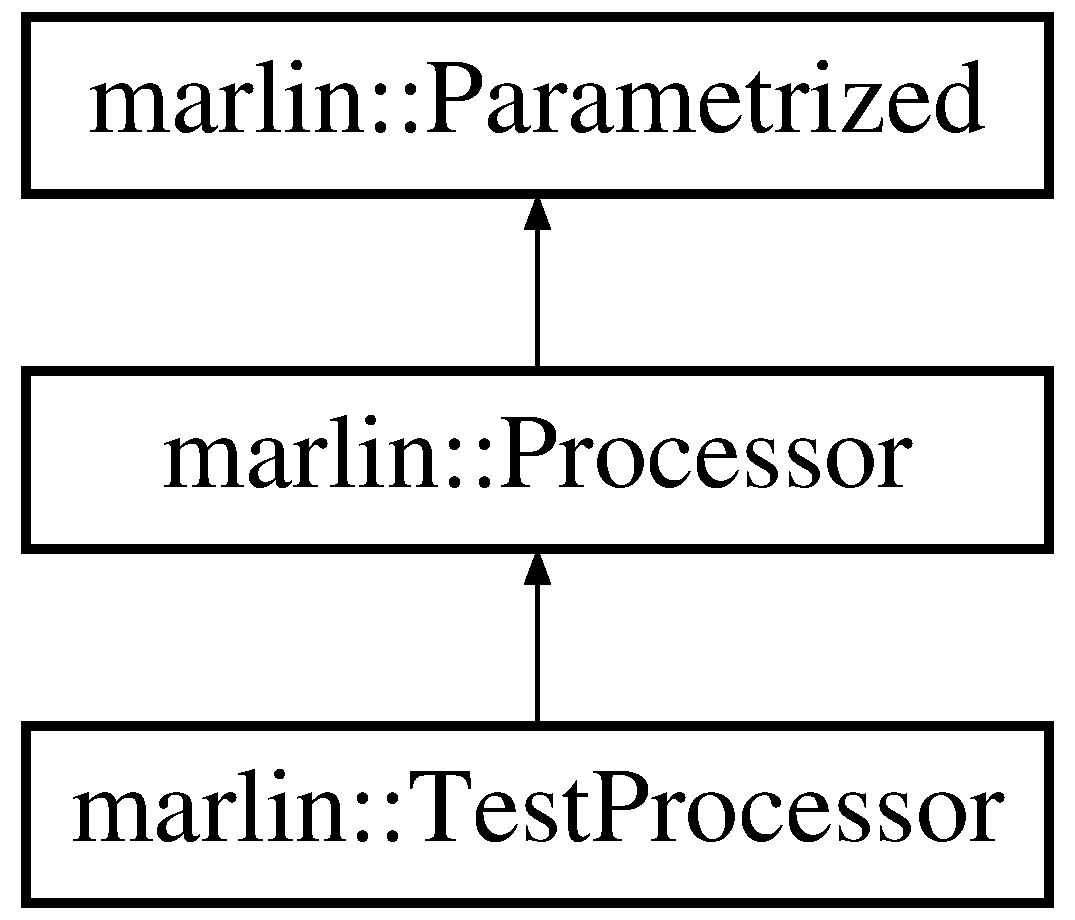
\includegraphics[height=3.000000cm]{classmarlin_1_1TestProcessor}
\end{center}
\end{figure}
\subsection*{Public Member Functions}
\begin{DoxyCompactItemize}
\item 
\mbox{\label{classmarlin_1_1TestProcessor_ac073820de55631e2c1cf84043b853345}} 
\textbf{ Processor} $\ast$ \textbf{ new\+Processor} ()
\begin{DoxyCompactList}\small\item\em Return a new instance of the processor (factory method) \end{DoxyCompactList}\item 
void \textbf{ init} ()
\begin{DoxyCompactList}\small\item\em Called at the begin of the job before anything is read. \end{DoxyCompactList}\item 
\mbox{\label{classmarlin_1_1TestProcessor_a4eed8ec8838445c9ca5261add8fc3112}} 
void \textbf{ process\+Run\+Header} (E\+V\+E\+N\+T\+::\+L\+C\+Run\+Header $\ast$run)
\begin{DoxyCompactList}\small\item\em Called for every run. \end{DoxyCompactList}\item 
\mbox{\label{classmarlin_1_1TestProcessor_a5ab65c443465d9407bd5adca1d798c59}} 
void \textbf{ process\+Event} (E\+V\+E\+N\+T\+::\+L\+C\+Event $\ast$evt)
\begin{DoxyCompactList}\small\item\em Called for every event -\/ the working horse. \end{DoxyCompactList}\item 
void \textbf{ check} (E\+V\+E\+N\+T\+::\+L\+C\+Event $\ast$evt)
\begin{DoxyCompactList}\small\item\em Called for every event -\/ right after \doxyref{process\+Event()}{p.}{classmarlin_1_1TestProcessor_a5ab65c443465d9407bd5adca1d798c59} has been called for this processor. \end{DoxyCompactList}\item 
\mbox{\label{classmarlin_1_1TestProcessor_adf788e37e471e1e6ff8a59c4db0afae0}} 
void \textbf{ end} ()
\begin{DoxyCompactList}\small\item\em Called after data processing for clean up. \end{DoxyCompactList}\end{DoxyCompactItemize}
\subsection*{Protected Member Functions}
\begin{DoxyCompactItemize}
\item 
void \textbf{ print\+End\+Message} () const
\begin{DoxyCompactList}\small\item\em Test method for const. \end{DoxyCompactList}\end{DoxyCompactItemize}
\subsection*{Protected Attributes}
\begin{DoxyCompactItemize}
\item 
\mbox{\label{classmarlin_1_1TestProcessor_a78908bd5f476c766d7708316d1cdcd0d}} 
int {\bfseries \+\_\+n\+Run} \{0\}
\item 
\mbox{\label{classmarlin_1_1TestProcessor_a3f819d54419105ef06c29307bc0410bf}} 
std\+::atomic\+\_\+int {\bfseries \+\_\+n\+Evt} \{0\}
\item 
\mbox{\label{classmarlin_1_1TestProcessor_a6efad1202492663ae5a3e0b818562614}} 
bool {\bfseries \+\_\+do\+Calibration} \{false\}
\end{DoxyCompactItemize}
\subsection*{Additional Inherited Members}


\subsection{Detailed Description}
Simple processor for testing. 

Writes something to stdout for every callbackmethod.

\subparagraph*{Input -\/ Prerequisites}

none

\subparagraph*{Output}

none

\begin{DoxyAuthor}{Author}
F. Gaede, D\+E\+SY 
\end{DoxyAuthor}
\begin{DoxyVersion}{Version}

\end{DoxyVersion}
\begin{DoxyParagraph}{Id}
Test\+Processor.\+h,v 1.\+7 2007-\/05-\/23 13\+:12\+:21 gaede Exp 
\end{DoxyParagraph}


\subsection{Member Function Documentation}
\mbox{\label{classmarlin_1_1TestProcessor_ae4c252ec319b9633c0132471c24cb3e8}} 
\index{marlin\+::\+Test\+Processor@{marlin\+::\+Test\+Processor}!check@{check}}
\index{check@{check}!marlin\+::\+Test\+Processor@{marlin\+::\+Test\+Processor}}
\subsubsection{check()}
{\footnotesize\ttfamily void marlin\+::\+Test\+Processor\+::check (\begin{DoxyParamCaption}\item[{E\+V\+E\+N\+T\+::\+L\+C\+Event $\ast$}]{ }\end{DoxyParamCaption})\hspace{0.3cm}{\ttfamily [virtual]}}



Called for every event -\/ right after \doxyref{process\+Event()}{p.}{classmarlin_1_1TestProcessor_a5ab65c443465d9407bd5adca1d798c59} has been called for this processor. 

Use to check processing and/or produce check plots. 

Reimplemented from \textbf{ marlin\+::\+Processor} \doxyref{}{p.}{classmarlin_1_1Processor_a1e2b7d44f9e69498fb4679cb9d2b0b3b}.



Referenced by new\+Processor().

\mbox{\label{classmarlin_1_1TestProcessor_a642eda7da954ecd815df99f25a1c946b}} 
\index{marlin\+::\+Test\+Processor@{marlin\+::\+Test\+Processor}!init@{init}}
\index{init@{init}!marlin\+::\+Test\+Processor@{marlin\+::\+Test\+Processor}}
\subsubsection{init()}
{\footnotesize\ttfamily void marlin\+::\+Test\+Processor\+::init (\begin{DoxyParamCaption}{ }\end{DoxyParamCaption})\hspace{0.3cm}{\ttfamily [virtual]}}



Called at the begin of the job before anything is read. 

Use to initialize the processor, e.\+g. book histograms. 

Reimplemented from \textbf{ marlin\+::\+Processor} \doxyref{}{p.}{classmarlin_1_1Processor_a8194fb92a428de40ea9d891c8c8aed6b}.



References marlin\+::\+Processor\+::name(), and marlin\+::\+Processor\+::parameters().



Referenced by new\+Processor().

\mbox{\label{classmarlin_1_1TestProcessor_ab7494182baf39229a6f96c8a794256ed}} 
\index{marlin\+::\+Test\+Processor@{marlin\+::\+Test\+Processor}!print\+End\+Message@{print\+End\+Message}}
\index{print\+End\+Message@{print\+End\+Message}!marlin\+::\+Test\+Processor@{marlin\+::\+Test\+Processor}}
\subsubsection{print\+End\+Message()}
{\footnotesize\ttfamily void marlin\+::\+Test\+Processor\+::print\+End\+Message (\begin{DoxyParamCaption}{ }\end{DoxyParamCaption}) const\hspace{0.3cm}{\ttfamily [protected]}}



Test method for const. 



Referenced by end(), and new\+Processor().



The documentation for this class was generated from the following file\+:\begin{DoxyCompactItemize}
\item 
Test\+Processor.\+cc\end{DoxyCompactItemize}

\section{marlin\+:\+:concurrency\+:\+:Thread\+Pool$<$ IN, O\+UT $>$ Class Template Reference}
\label{classmarlin_1_1concurrency_1_1ThreadPool}\index{marlin\+::concurrency\+::\+Thread\+Pool$<$ I\+N, O\+U\+T $>$@{marlin\+::concurrency\+::\+Thread\+Pool$<$ I\+N, O\+U\+T $>$}}


\doxyref{Thread\+Pool}{p.}{classmarlin_1_1concurrency_1_1ThreadPool} class The template parameter T is the type of data to enqueue and process in worker threads.  




{\ttfamily \#include $<$Thread\+Pool.\+h$>$}

\subsection*{Public Types}
\begin{DoxyCompactItemize}
\item 
enum \textbf{ Push\+Policy} \{ \textbf{ Push\+Policy\+::\+Blocking}, 
\textbf{ Push\+Policy\+::\+Throw\+If\+Full}
 \}\begin{DoxyCompactList}\small\item\em Push\+Policy enumerator. \end{DoxyCompactList}
\item 
\mbox{\label{classmarlin_1_1concurrency_1_1ThreadPool_a728b47339b03f6dc64a45bddc7b213ab}} 
using {\bfseries Queue\+Type} = \textbf{ Queue}$<$ \textbf{ Queue\+Element}$<$ IN, O\+UT $>$ $>$
\item 
\mbox{\label{classmarlin_1_1concurrency_1_1ThreadPool_a690f1a68f35e294d8da5d6af55904649}} 
using {\bfseries Pool\+Type} = std\+::vector$<$ std\+::shared\+\_\+ptr$<$ \textbf{ Worker}$<$ IN, O\+UT $>$ $>$$>$
\item 
\mbox{\label{classmarlin_1_1concurrency_1_1ThreadPool_a5233168cd4afe40c3c98ffcd54ebd560}} 
using {\bfseries Promise} = std\+::shared\+\_\+ptr$<$ std\+::promise$<$ O\+UT $>$ $>$
\item 
\mbox{\label{classmarlin_1_1concurrency_1_1ThreadPool_a016f81f23b6dfc5d9312e8d2ecdaf520}} 
using {\bfseries Future} = std\+::future$<$ O\+UT $>$
\item 
\mbox{\label{classmarlin_1_1concurrency_1_1ThreadPool_ac6056a836a7bff61e8438aa72d01edfc}} 
using {\bfseries Push\+Result} = std\+::pair$<$ Promise, Future $>$
\end{DoxyCompactItemize}
\subsection*{Public Member Functions}
\begin{DoxyCompactItemize}
\item 
\mbox{\label{classmarlin_1_1concurrency_1_1ThreadPool_aebc1ddd5d4d9767a3885b667a51261ca}} 
{\bfseries Thread\+Pool} (const \textbf{ Thread\+Pool} \&)=delete
\item 
\mbox{\label{classmarlin_1_1concurrency_1_1ThreadPool_a42f331c64fb54362f91ecf9e10cd5412}} 
{\bfseries Thread\+Pool} (\textbf{ Thread\+Pool} \&\&)=delete
\item 
\mbox{\label{classmarlin_1_1concurrency_1_1ThreadPool_af46f66c0c8442e02e0dad022b7c956c4}} 
\textbf{ Thread\+Pool} \& {\bfseries operator=} (const \textbf{ Thread\+Pool} \&)=delete
\item 
\mbox{\label{classmarlin_1_1concurrency_1_1ThreadPool_ab6822bc8aee4922871ad77628db72961}} 
\textbf{ Thread\+Pool} \& {\bfseries operator=} (\textbf{ Thread\+Pool} \&\&)=delete
\item 
\mbox{\label{classmarlin_1_1concurrency_1_1ThreadPool_ae4ec499f35e1d37c8c32e03442a59ebe}} 
\textbf{ $\sim$\+Thread\+Pool} ()
\begin{DoxyCompactList}\small\item\em Destructor. \end{DoxyCompactList}\item 
{\footnotesize template$<$typename W\+O\+R\+K\+ER , typename ... Args$>$ }\\void \textbf{ add\+Worker} (Args \&\&...args)
\begin{DoxyCompactList}\small\item\em Add a new worker thread. \end{DoxyCompactList}\item 
\mbox{\label{classmarlin_1_1concurrency_1_1ThreadPool_a1cddd87b3820d13b99e4f5fae79cc006}} 
void \textbf{ start} ()
\begin{DoxyCompactList}\small\item\em Start the worker threads. \end{DoxyCompactList}\item 
\mbox{\label{classmarlin_1_1concurrency_1_1ThreadPool_aad45418d2b691dc4703b880e6d797b4d}} 
std\+::size\+\_\+t \textbf{ size} () const
\begin{DoxyCompactList}\small\item\em Get the thread pool size. \end{DoxyCompactList}\item 
\mbox{\label{classmarlin_1_1concurrency_1_1ThreadPool_a0a5a9bec06e7984168530bdfb4cf0242}} 
std\+::size\+\_\+t \textbf{ n\+Waiting} () const
\begin{DoxyCompactList}\small\item\em Get the number of waiting threads. \end{DoxyCompactList}\item 
\mbox{\label{classmarlin_1_1concurrency_1_1ThreadPool_a3be8a902065c31077ef345cd03036d01}} 
std\+::size\+\_\+t \textbf{ n\+Running} () const
\begin{DoxyCompactList}\small\item\em Get the number of threads currently handling a task. \end{DoxyCompactList}\item 
\mbox{\label{classmarlin_1_1concurrency_1_1ThreadPool_a2ddd44c5ce7f7cd28e6acf9c0c4cbb0a}} 
std\+::size\+\_\+t \textbf{ free\+Slots} () const
\begin{DoxyCompactList}\small\item\em Get the number of free slots in the task queue. \end{DoxyCompactList}\item 
\mbox{\label{classmarlin_1_1concurrency_1_1ThreadPool_a2ca960e716e99fd64eca3a107a43b4b1}} 
bool \textbf{ is\+Queue\+Empty} () const
\begin{DoxyCompactList}\small\item\em Whether the queue is empty. \end{DoxyCompactList}\item 
\mbox{\label{classmarlin_1_1concurrency_1_1ThreadPool_a68cc65198d64d5f32ba889b1e0c1754b}} 
void \textbf{ clear\+Queue} ()
\begin{DoxyCompactList}\small\item\em Clear the queue. \end{DoxyCompactList}\item 
void \textbf{ set\+Max\+Queue\+Size} (std\+::size\+\_\+t max\+Queue\+Size)
\begin{DoxyCompactList}\small\item\em Set the maximum queue size. \end{DoxyCompactList}\item 
void \textbf{ set\+Accept\+Push} (bool accept)
\begin{DoxyCompactList}\small\item\em Set whether the thread pool accept data push. \end{DoxyCompactList}\item 
\mbox{\label{classmarlin_1_1concurrency_1_1ThreadPool_a300c5d5df797a2a04d8c674c6dc3f348}} 
bool \textbf{ accept\+Push} () const
\begin{DoxyCompactList}\small\item\em Whether the thread pool accepts data push. \end{DoxyCompactList}\item 
\mbox{\label{classmarlin_1_1concurrency_1_1ThreadPool_ae5503a48ee34adcf03a7a4e53a7d75a0}} 
bool \textbf{ active} () const
\begin{DoxyCompactList}\small\item\em Whether the thread pool is active, meaning that the queue is not empty or at least one worker is active. \end{DoxyCompactList}\item 
void \textbf{ stop} (bool clear=true)
\begin{DoxyCompactList}\small\item\em Stop the thread pool. \end{DoxyCompactList}\item 
{\footnotesize template$<$class  = typename std\+::enable\+\_\+if$<$not std\+::is\+\_\+same$<$\+I\+N,void$>$\+::value$>$\+::type$>$ }\\Push\+Result \textbf{ push} (\textbf{ Push\+Policy} policy, IN \&\&input)
\begin{DoxyCompactList}\small\item\em Push a new task in the task queue. \end{DoxyCompactList}\end{DoxyCompactItemize}
\subsection*{Friends}
\begin{DoxyCompactItemize}
\item 
\mbox{\label{classmarlin_1_1concurrency_1_1ThreadPool_a491b906d2052cbe1c394c75e0e2d72a5}} 
class {\bfseries Worker$<$ I\+N, O\+U\+T $>$}
\end{DoxyCompactItemize}


\subsection{Detailed Description}
\subsubsection*{template$<$typename IN, typename O\+UT$>$\newline
class marlin\+::concurrency\+::\+Thread\+Pool$<$ I\+N, O\+U\+T $>$}

\doxyref{Thread\+Pool}{p.}{classmarlin_1_1concurrency_1_1ThreadPool} class The template parameter T is the type of data to enqueue and process in worker threads. 

\subsection{Member Enumeration Documentation}
\mbox{\label{classmarlin_1_1concurrency_1_1ThreadPool_aa812123afc377d93ad4d91cd6b3daed2}} 
\index{marlin\+::concurrency\+::\+Thread\+Pool@{marlin\+::concurrency\+::\+Thread\+Pool}!Push\+Policy@{Push\+Policy}}
\index{Push\+Policy@{Push\+Policy}!marlin\+::concurrency\+::\+Thread\+Pool@{marlin\+::concurrency\+::\+Thread\+Pool}}
\subsubsection{Push\+Policy}
{\footnotesize\ttfamily template$<$typename IN, typename O\+UT$>$ \\
enum \textbf{ marlin\+::concurrency\+::\+Thread\+Pool\+::\+Push\+Policy}\hspace{0.3cm}{\ttfamily [strong]}}



Push\+Policy enumerator. 

\begin{DoxyEnumFields}{Enumerator}
\raisebox{\heightof{T}}[0pt][0pt]{\index{Blocking@{Blocking}!marlin\+::concurrency\+::\+Thread\+Pool@{marlin\+::concurrency\+::\+Thread\+Pool}}\index{marlin\+::concurrency\+::\+Thread\+Pool@{marlin\+::concurrency\+::\+Thread\+Pool}!Blocking@{Blocking}}}\mbox{\label{classmarlin_1_1concurrency_1_1ThreadPool_aa812123afc377d93ad4d91cd6b3daed2abd0ca6be53b0f3d2886fd53fcb52574e}} 
Blocking&Block until a slot is free in the queue. \\
\hline

\raisebox{\heightof{T}}[0pt][0pt]{\index{Throw\+If\+Full@{Throw\+If\+Full}!marlin\+::concurrency\+::\+Thread\+Pool@{marlin\+::concurrency\+::\+Thread\+Pool}}\index{marlin\+::concurrency\+::\+Thread\+Pool@{marlin\+::concurrency\+::\+Thread\+Pool}!Throw\+If\+Full@{Throw\+If\+Full}}}\mbox{\label{classmarlin_1_1concurrency_1_1ThreadPool_aa812123afc377d93ad4d91cd6b3daed2afa9df3c61a331de501ef79fdfe81ad4a}} 
Throw\+If\+Full&Throw an exception if the queue is full. \\
\hline

\end{DoxyEnumFields}


\subsection{Member Function Documentation}
\mbox{\label{classmarlin_1_1concurrency_1_1ThreadPool_aaf7bc6b1caed163cb2f54aa35c7246da}} 
\index{marlin\+::concurrency\+::\+Thread\+Pool@{marlin\+::concurrency\+::\+Thread\+Pool}!add\+Worker@{add\+Worker}}
\index{add\+Worker@{add\+Worker}!marlin\+::concurrency\+::\+Thread\+Pool@{marlin\+::concurrency\+::\+Thread\+Pool}}
\subsubsection{add\+Worker()}
{\footnotesize\ttfamily template$<$typename IN , typename O\+UT $>$ \\
template$<$typename W\+O\+R\+K\+ER , typename ... Args$>$ \\
void \textbf{ marlin\+::concurrency\+::\+Thread\+Pool}$<$ IN, O\+UT $>$\+::add\+Worker (\begin{DoxyParamCaption}\item[{Args \&\&...}]{args }\end{DoxyParamCaption})\hspace{0.3cm}{\ttfamily [inline]}}



Add a new worker thread. 


\begin{DoxyParams}{Parameters}
{\em args} & arguments to pass to worker constructor \\
\hline
\end{DoxyParams}
\mbox{\label{classmarlin_1_1concurrency_1_1ThreadPool_a60d1d6077b516d0aa5a2244c378e7979}} 
\index{marlin\+::concurrency\+::\+Thread\+Pool@{marlin\+::concurrency\+::\+Thread\+Pool}!push@{push}}
\index{push@{push}!marlin\+::concurrency\+::\+Thread\+Pool@{marlin\+::concurrency\+::\+Thread\+Pool}}
\subsubsection{push()}
{\footnotesize\ttfamily template$<$typename IN, typename O\+UT $>$ \\
template$<$class $>$ \\
\textbf{ Thread\+Pool}$<$ IN, O\+UT $>$\+::Push\+Result \textbf{ marlin\+::concurrency\+::\+Thread\+Pool}$<$ IN, O\+UT $>$\+::push (\begin{DoxyParamCaption}\item[{\textbf{ Push\+Policy}}]{policy,  }\item[{IN \&\&}]{input }\end{DoxyParamCaption})\hspace{0.3cm}{\ttfamily [inline]}}



Push a new task in the task queue. 

See Push\+Policy for runtime behavior of enqueuing.


\begin{DoxyParams}{Parameters}
{\em policy} & the push policy \\
\hline
{\em } & \\
\hline
\end{DoxyParams}
\mbox{\label{classmarlin_1_1concurrency_1_1ThreadPool_af1b937d90dfd341103aa33eab98b136e}} 
\index{marlin\+::concurrency\+::\+Thread\+Pool@{marlin\+::concurrency\+::\+Thread\+Pool}!set\+Accept\+Push@{set\+Accept\+Push}}
\index{set\+Accept\+Push@{set\+Accept\+Push}!marlin\+::concurrency\+::\+Thread\+Pool@{marlin\+::concurrency\+::\+Thread\+Pool}}
\subsubsection{set\+Accept\+Push()}
{\footnotesize\ttfamily template$<$typename IN , typename O\+UT $>$ \\
void \textbf{ marlin\+::concurrency\+::\+Thread\+Pool}$<$ IN, O\+UT $>$\+::set\+Accept\+Push (\begin{DoxyParamCaption}\item[{bool}]{accept }\end{DoxyParamCaption})\hspace{0.3cm}{\ttfamily [inline]}}



Set whether the thread pool accept data push. 


\begin{DoxyParams}{Parameters}
{\em accept} & whether to accept data push \\
\hline
\end{DoxyParams}
\mbox{\label{classmarlin_1_1concurrency_1_1ThreadPool_ad665133f4e606e22dd13559601dfccbb}} 
\index{marlin\+::concurrency\+::\+Thread\+Pool@{marlin\+::concurrency\+::\+Thread\+Pool}!set\+Max\+Queue\+Size@{set\+Max\+Queue\+Size}}
\index{set\+Max\+Queue\+Size@{set\+Max\+Queue\+Size}!marlin\+::concurrency\+::\+Thread\+Pool@{marlin\+::concurrency\+::\+Thread\+Pool}}
\subsubsection{set\+Max\+Queue\+Size()}
{\footnotesize\ttfamily template$<$typename IN , typename O\+UT $>$ \\
void \textbf{ marlin\+::concurrency\+::\+Thread\+Pool}$<$ IN, O\+UT $>$\+::set\+Max\+Queue\+Size (\begin{DoxyParamCaption}\item[{std\+::size\+\_\+t}]{max\+Queue\+Size }\end{DoxyParamCaption})\hspace{0.3cm}{\ttfamily [inline]}}



Set the maximum queue size. 


\begin{DoxyParams}{Parameters}
{\em max\+Queue\+Size} & the maximum queue size \\
\hline
\end{DoxyParams}
\mbox{\label{classmarlin_1_1concurrency_1_1ThreadPool_acbaed70df966cb82296cf7ba794e6705}} 
\index{marlin\+::concurrency\+::\+Thread\+Pool@{marlin\+::concurrency\+::\+Thread\+Pool}!stop@{stop}}
\index{stop@{stop}!marlin\+::concurrency\+::\+Thread\+Pool@{marlin\+::concurrency\+::\+Thread\+Pool}}
\subsubsection{stop()}
{\footnotesize\ttfamily template$<$typename IN , typename O\+UT $>$ \\
void \textbf{ marlin\+::concurrency\+::\+Thread\+Pool}$<$ IN, O\+UT $>$\+::stop (\begin{DoxyParamCaption}\item[{bool}]{clear = {\ttfamily true} }\end{DoxyParamCaption})\hspace{0.3cm}{\ttfamily [inline]}}



Stop the thread pool. 

If the flag clear is set to true, the task queue is cleared. The threads are joined and the pool is clear. As no threads remains in the pool, the pool is not reusable. Thus this method must be called for performing a proper program termination before exiting


\begin{DoxyParams}{Parameters}
{\em clear} & whether the task queue should be cleared \\
\hline
\end{DoxyParams}


Referenced by marlin\+::concurrency\+::\+Thread\+Pool$<$ Input\+Type, Output\+Type $>$\+::$\sim$\+Thread\+Pool().



The documentation for this class was generated from the following file\+:\begin{DoxyCompactItemize}
\item 
Thread\+Pool.\+h\end{DoxyCompactItemize}

\section{Ti\+Xml\+Attribute Class Reference}
\label{classTiXmlAttribute}\index{Ti\+Xml\+Attribute@{Ti\+Xml\+Attribute}}


An attribute is a name-\/value pair.  




{\ttfamily \#include $<$tinyxml.\+h$>$}

Inheritance diagram for Ti\+Xml\+Attribute\+:\begin{figure}[H]
\begin{center}
\leavevmode
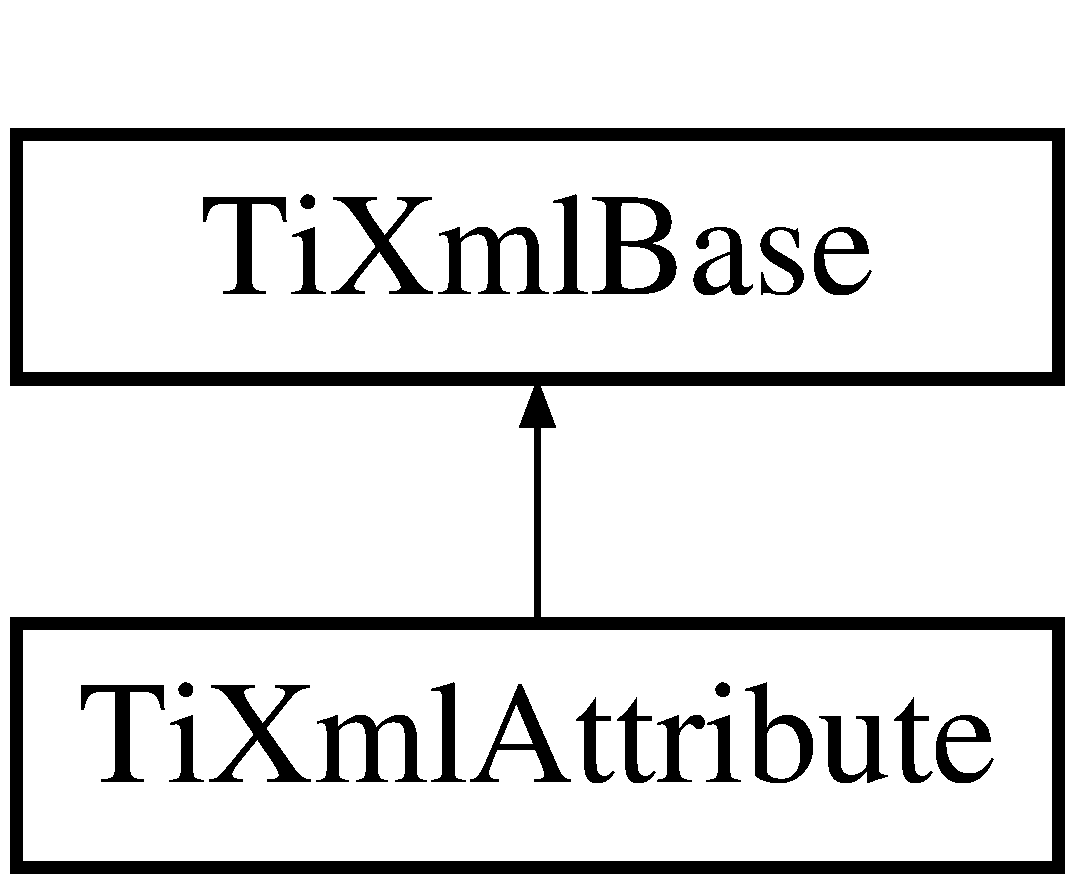
\includegraphics[height=2.000000cm]{classTiXmlAttribute}
\end{center}
\end{figure}
\subsection*{Public Member Functions}
\begin{DoxyCompactItemize}
\item 
\mbox{\label{classTiXmlAttribute_a9cfa3c8179873fd485d83003b114f8e1}} 
\textbf{ Ti\+Xml\+Attribute} ()
\begin{DoxyCompactList}\small\item\em Construct an empty attribute. \end{DoxyCompactList}\item 
\mbox{\label{classTiXmlAttribute_a052213522caac3979960e0714063861d}} 
\textbf{ Ti\+Xml\+Attribute} (const std\+::string \&\+\_\+name, const std\+::string \&\+\_\+value)
\begin{DoxyCompactList}\small\item\em std\+::string constructor. \end{DoxyCompactList}\item 
\mbox{\label{classTiXmlAttribute_a759d0b76fb8fcf765ecab243bc14f05e}} 
\textbf{ Ti\+Xml\+Attribute} (const char $\ast$\+\_\+name, const char $\ast$\+\_\+value)
\begin{DoxyCompactList}\small\item\em Construct an attribute with a name and value. \end{DoxyCompactList}\item 
\mbox{\label{classTiXmlAttribute_a008ef948268ee752b58c60d63d84bb01}} 
const char $\ast$ \textbf{ Name} () const
\begin{DoxyCompactList}\small\item\em Return the name of this attribute. \end{DoxyCompactList}\item 
\mbox{\label{classTiXmlAttribute_ac9f0b56fcacbedb6eb49e5f282bef014}} 
const char $\ast$ \textbf{ Value} () const
\begin{DoxyCompactList}\small\item\em Return the value of this attribute. \end{DoxyCompactList}\item 
\mbox{\label{classTiXmlAttribute_af70a11c3a0c07e61bd6e215f1f9b24e9}} 
const std\+::string \& \textbf{ Value\+Str} () const
\begin{DoxyCompactList}\small\item\em Return the value of this attribute. \end{DoxyCompactList}\item 
\mbox{\label{classTiXmlAttribute_ac8501370b065df31a35003c81d87cef2}} 
int \textbf{ Int\+Value} () const
\begin{DoxyCompactList}\small\item\em Return the value of this attribute, converted to an integer. \end{DoxyCompactList}\item 
\mbox{\label{classTiXmlAttribute_a8cca240fb2a7130c87b0fc6156e8b34f}} 
double \textbf{ Double\+Value} () const
\begin{DoxyCompactList}\small\item\em Return the value of this attribute, converted to a double. \end{DoxyCompactList}\item 
\mbox{\label{classTiXmlAttribute_a2bd49ec37463a0a2d081e6587f8b89b8}} 
const T\+I\+X\+M\+L\+\_\+\+S\+T\+R\+I\+NG \& {\bfseries Name\+T\+Str} () const
\item 
int \textbf{ Query\+Int\+Value} (int $\ast$\+\_\+value) const
\begin{DoxyCompactList}\small\item\em Query\+Int\+Value examines the value string. \end{DoxyCompactList}\item 
\mbox{\label{classTiXmlAttribute_a6fa41b710c1b79de37a97004aa600c06}} 
int \textbf{ Query\+Double\+Value} (double $\ast$\+\_\+value) const
\begin{DoxyCompactList}\small\item\em Query\+Double\+Value examines the value string. See \doxyref{Query\+Int\+Value()}{p.}{classTiXmlAttribute_a6caa8090d2fbb7966700a16e45ed33de}. \end{DoxyCompactList}\item 
\mbox{\label{classTiXmlAttribute_ab7fa3d21ff8d7c5764cf9af15b667a99}} 
void \textbf{ Set\+Name} (const char $\ast$\+\_\+name)
\begin{DoxyCompactList}\small\item\em Set the name of this attribute. \end{DoxyCompactList}\item 
\mbox{\label{classTiXmlAttribute_a2dae44178f668b3cb48101be4f2236a0}} 
void \textbf{ Set\+Value} (const char $\ast$\+\_\+value)
\begin{DoxyCompactList}\small\item\em Set the value. \end{DoxyCompactList}\item 
\mbox{\label{classTiXmlAttribute_a7e065df640116a62ea4f4b7da5449cc8}} 
void \textbf{ Set\+Int\+Value} (int \+\_\+value)
\begin{DoxyCompactList}\small\item\em Set the value from an integer. \end{DoxyCompactList}\item 
\mbox{\label{classTiXmlAttribute_a0316da31373496c4368ad549bf711394}} 
void \textbf{ Set\+Double\+Value} (double \+\_\+value)
\begin{DoxyCompactList}\small\item\em Set the value from a double. \end{DoxyCompactList}\item 
\mbox{\label{classTiXmlAttribute_ab296ff0c9a8c701055cd257a8a976e57}} 
void \textbf{ Set\+Name} (const std\+::string \&\+\_\+name)
\begin{DoxyCompactList}\small\item\em S\+TL std\+::string form. \end{DoxyCompactList}\item 
\mbox{\label{classTiXmlAttribute_ab43f67a0cc3ec1d80e62606500f0925f}} 
void \textbf{ Set\+Value} (const std\+::string \&\+\_\+value)
\begin{DoxyCompactList}\small\item\em S\+TL std\+::string form. \end{DoxyCompactList}\item 
\mbox{\label{classTiXmlAttribute_af2e78f1ba9ed56a26ddc80614ed1c393}} 
const \textbf{ Ti\+Xml\+Attribute} $\ast$ \textbf{ Next} () const
\begin{DoxyCompactList}\small\item\em Get the next sibling attribute in the D\+OM. Returns null at end. \end{DoxyCompactList}\item 
\mbox{\label{classTiXmlAttribute_a138320aa7793b148ba7e5bd0a0ea4db6}} 
\textbf{ Ti\+Xml\+Attribute} $\ast$ {\bfseries Next} ()
\item 
\mbox{\label{classTiXmlAttribute_afc7bbfdf83d59fbc4ff5e283d27b5d7d}} 
const \textbf{ Ti\+Xml\+Attribute} $\ast$ \textbf{ Previous} () const
\begin{DoxyCompactList}\small\item\em Get the previous sibling attribute in the D\+OM. Returns null at beginning. \end{DoxyCompactList}\item 
\mbox{\label{classTiXmlAttribute_ae4dabc932cba945ed1e92fec5f121193}} 
\textbf{ Ti\+Xml\+Attribute} $\ast$ {\bfseries Previous} ()
\item 
\mbox{\label{classTiXmlAttribute_a51eef33c2cdd55831447af46be0baf8b}} 
bool {\bfseries operator==} (const \textbf{ Ti\+Xml\+Attribute} \&rhs) const
\item 
\mbox{\label{classTiXmlAttribute_a80dcb758cc5ab27ce9865301e2da1335}} 
bool {\bfseries operator$<$} (const \textbf{ Ti\+Xml\+Attribute} \&rhs) const
\item 
\mbox{\label{classTiXmlAttribute_a697c2dde7ac60fccaa7049cee906eb3e}} 
bool {\bfseries operator$>$} (const \textbf{ Ti\+Xml\+Attribute} \&rhs) const
\item 
\mbox{\label{classTiXmlAttribute_ad62774421b814894b995af3b5d231dda}} 
virtual const char $\ast$ {\bfseries Parse} (const char $\ast$p, \textbf{ Ti\+Xml\+Parsing\+Data} $\ast$data, Ti\+Xml\+Encoding encoding)
\item 
virtual void \textbf{ Print} (F\+I\+LE $\ast$cfile, int depth) const
\begin{DoxyCompactList}\small\item\em All Tiny\+Xml classes can print themselves to a filestream or the string class (\doxyref{Ti\+Xml\+String}{p.}{classTiXmlString} in non-\/\+S\+TL mode, std\+::string in S\+TL mode.) Either or both cfile and str can be null. \end{DoxyCompactList}\item 
\mbox{\label{classTiXmlAttribute_a5c8f72a7d1a49972434d45f4c2889e0e}} 
void {\bfseries Print} (F\+I\+LE $\ast$cfile, int depth, T\+I\+X\+M\+L\+\_\+\+S\+T\+R\+I\+NG $\ast$str) const
\item 
\mbox{\label{classTiXmlAttribute_ac12a94d4548302afb12f488ba101f7d1}} 
void {\bfseries Set\+Document} (\textbf{ Ti\+Xml\+Document} $\ast$doc)
\end{DoxyCompactItemize}
\subsection*{Friends}
\begin{DoxyCompactItemize}
\item 
\mbox{\label{classTiXmlAttribute_a35a7b7f89f708527677d5078d41ce0bf}} 
class {\bfseries Ti\+Xml\+Attribute\+Set}
\end{DoxyCompactItemize}
\subsection*{Additional Inherited Members}


\subsection{Detailed Description}
An attribute is a name-\/value pair. 

Elements have an arbitrary number of attributes, each with a unique name.

\begin{DoxyNote}{Note}
The attributes are not Ti\+Xml\+Nodes, since they are not part of the tiny\+X\+ML document object model. There are other suggested ways to look at this problem. 
\end{DoxyNote}


\subsection{Member Function Documentation}
\mbox{\label{classTiXmlAttribute_a68ae373e03b9c35be4c9d0c3c233b894}} 
\index{Ti\+Xml\+Attribute@{Ti\+Xml\+Attribute}!Print@{Print}}
\index{Print@{Print}!Ti\+Xml\+Attribute@{Ti\+Xml\+Attribute}}
\subsubsection{Print()}
{\footnotesize\ttfamily virtual void Ti\+Xml\+Attribute\+::\+Print (\begin{DoxyParamCaption}\item[{F\+I\+LE $\ast$}]{cfile,  }\item[{int}]{depth }\end{DoxyParamCaption}) const\hspace{0.3cm}{\ttfamily [inline]}, {\ttfamily [virtual]}}



All Tiny\+Xml classes can print themselves to a filestream or the string class (\doxyref{Ti\+Xml\+String}{p.}{classTiXmlString} in non-\/\+S\+TL mode, std\+::string in S\+TL mode.) Either or both cfile and str can be null. 

This is a formatted print, and will insert tabs and newlines.

(For an unformatted stream, use the $<$$<$ operator.) 

Implements \textbf{ Ti\+Xml\+Base} \doxyref{}{p.}{classTiXmlBase_a0de56b3f2ef14c65091a3b916437b512}.



Referenced by Previous().

\mbox{\label{classTiXmlAttribute_a6caa8090d2fbb7966700a16e45ed33de}} 
\index{Ti\+Xml\+Attribute@{Ti\+Xml\+Attribute}!Query\+Int\+Value@{Query\+Int\+Value}}
\index{Query\+Int\+Value@{Query\+Int\+Value}!Ti\+Xml\+Attribute@{Ti\+Xml\+Attribute}}
\subsubsection{Query\+Int\+Value()}
{\footnotesize\ttfamily int Ti\+Xml\+Attribute\+::\+Query\+Int\+Value (\begin{DoxyParamCaption}\item[{int $\ast$}]{\+\_\+value }\end{DoxyParamCaption}) const}



Query\+Int\+Value examines the value string. 

It is an alternative to the \doxyref{Int\+Value()}{p.}{classTiXmlAttribute_ac8501370b065df31a35003c81d87cef2} method with richer error checking. If the value is an integer, it is stored in \textquotesingle{}value\textquotesingle{} and the call returns T\+I\+X\+M\+L\+\_\+\+S\+U\+C\+C\+E\+SS. If it is not an integer, it returns T\+I\+X\+M\+L\+\_\+\+W\+R\+O\+N\+G\+\_\+\+T\+Y\+PE.

A specialized but useful call. Note that for success it returns 0, which is the opposite of almost all other Tiny\+Xml calls. 

Referenced by Ti\+Xml\+Element\+::\+Query\+Int\+Attribute().



The documentation for this class was generated from the following files\+:\begin{DoxyCompactItemize}
\item 
tinyxml.\+h\item 
tinyxml.\+cc\item 
tinyxmlparser.\+cc\end{DoxyCompactItemize}

\section{Ti\+Xml\+Attribute\+Set Class Reference}
\label{classTiXmlAttributeSet}\index{Ti\+Xml\+Attribute\+Set@{Ti\+Xml\+Attribute\+Set}}
\subsection*{Public Member Functions}
\begin{DoxyCompactItemize}
\item 
\mbox{\label{classTiXmlAttributeSet_a745e50ddaae3bee93e4589321e0b9c1a}} 
void {\bfseries Add} (\textbf{ Ti\+Xml\+Attribute} $\ast$attribute)
\item 
\mbox{\label{classTiXmlAttributeSet_a924a73d071f2573f9060f0be57879c57}} 
void {\bfseries Remove} (\textbf{ Ti\+Xml\+Attribute} $\ast$attribute)
\item 
\mbox{\label{classTiXmlAttributeSet_a85dfd2b5bae45c94334dced146f5c11a}} 
const \textbf{ Ti\+Xml\+Attribute} $\ast$ {\bfseries First} () const
\item 
\mbox{\label{classTiXmlAttributeSet_a99703bb08ca2aece2d7ef835de339ba0}} 
\textbf{ Ti\+Xml\+Attribute} $\ast$ {\bfseries First} ()
\item 
\mbox{\label{classTiXmlAttributeSet_a3b0d49f3802effcf377f32d9a359302c}} 
const \textbf{ Ti\+Xml\+Attribute} $\ast$ {\bfseries Last} () const
\item 
\mbox{\label{classTiXmlAttributeSet_ab4c4edfb2d74f6ea31aae096743bd6e0}} 
\textbf{ Ti\+Xml\+Attribute} $\ast$ {\bfseries Last} ()
\item 
\mbox{\label{classTiXmlAttributeSet_a39e9f5ed5ebbf02e059dd39cfa6c5052}} 
const \textbf{ Ti\+Xml\+Attribute} $\ast$ {\bfseries Find} (const char $\ast$\+\_\+name) const
\item 
\mbox{\label{classTiXmlAttributeSet_a2f210bed54c832adf1683c44c35727b9}} 
\textbf{ Ti\+Xml\+Attribute} $\ast$ {\bfseries Find} (const char $\ast$\+\_\+name)
\item 
\mbox{\label{classTiXmlAttributeSet_a49280440d5168e23b531e64afd399e50}} 
const \textbf{ Ti\+Xml\+Attribute} $\ast$ {\bfseries Find} (const std\+::string \&\+\_\+name) const
\item 
\mbox{\label{classTiXmlAttributeSet_ab154233f8ecffc0ee0c77a045fa9e69b}} 
\textbf{ Ti\+Xml\+Attribute} $\ast$ {\bfseries Find} (const std\+::string \&\+\_\+name)
\end{DoxyCompactItemize}


The documentation for this class was generated from the following files\+:\begin{DoxyCompactItemize}
\item 
tinyxml.\+h\item 
tinyxml.\+cc\end{DoxyCompactItemize}

\section{Ti\+Xml\+Base Class Reference}
\label{classTiXmlBase}\index{Ti\+Xml\+Base@{Ti\+Xml\+Base}}


\doxyref{Ti\+Xml\+Base}{p.}{classTiXmlBase} is a base class for every class in Tiny\+Xml.  




{\ttfamily \#include $<$tinyxml.\+h$>$}

Inheritance diagram for Ti\+Xml\+Base\+:\begin{figure}[H]
\begin{center}
\leavevmode
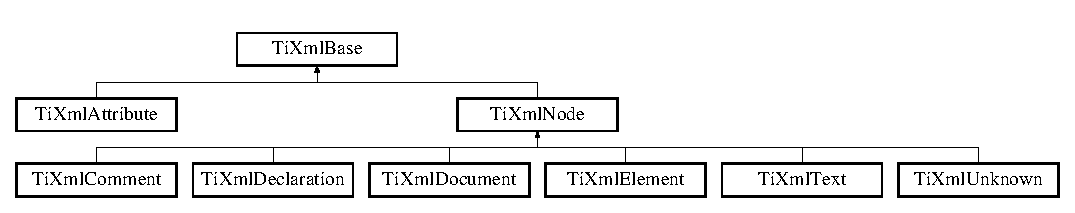
\includegraphics[height=2.413793cm]{classTiXmlBase}
\end{center}
\end{figure}
\subsection*{Public Types}
\begin{DoxyCompactItemize}
\item 
\mbox{\label{classTiXmlBase_a9a7e9344415956ab96e8c75f6a0bbd48}} 
enum \{ \newline
{\bfseries T\+I\+X\+M\+L\+\_\+\+N\+O\+\_\+\+E\+R\+R\+OR} = 0, 
{\bfseries T\+I\+X\+M\+L\+\_\+\+E\+R\+R\+OR}, 
{\bfseries T\+I\+X\+M\+L\+\_\+\+E\+R\+R\+O\+R\+\_\+\+O\+P\+E\+N\+I\+N\+G\+\_\+\+F\+I\+LE}, 
{\bfseries T\+I\+X\+M\+L\+\_\+\+E\+R\+R\+O\+R\+\_\+\+O\+U\+T\+\_\+\+O\+F\+\_\+\+M\+E\+M\+O\+RY}, 
\newline
{\bfseries T\+I\+X\+M\+L\+\_\+\+E\+R\+R\+O\+R\+\_\+\+P\+A\+R\+S\+I\+N\+G\+\_\+\+E\+L\+E\+M\+E\+NT}, 
{\bfseries T\+I\+X\+M\+L\+\_\+\+E\+R\+R\+O\+R\+\_\+\+F\+A\+I\+L\+E\+D\+\_\+\+T\+O\+\_\+\+R\+E\+A\+D\+\_\+\+E\+L\+E\+M\+E\+N\+T\+\_\+\+N\+A\+ME}, 
{\bfseries T\+I\+X\+M\+L\+\_\+\+E\+R\+R\+O\+R\+\_\+\+R\+E\+A\+D\+I\+N\+G\+\_\+\+E\+L\+E\+M\+E\+N\+T\+\_\+\+V\+A\+L\+UE}, 
{\bfseries T\+I\+X\+M\+L\+\_\+\+E\+R\+R\+O\+R\+\_\+\+R\+E\+A\+D\+I\+N\+G\+\_\+\+A\+T\+T\+R\+I\+B\+U\+T\+ES}, 
\newline
{\bfseries T\+I\+X\+M\+L\+\_\+\+E\+R\+R\+O\+R\+\_\+\+P\+A\+R\+S\+I\+N\+G\+\_\+\+E\+M\+P\+TY}, 
{\bfseries T\+I\+X\+M\+L\+\_\+\+E\+R\+R\+O\+R\+\_\+\+R\+E\+A\+D\+I\+N\+G\+\_\+\+E\+N\+D\+\_\+\+T\+AG}, 
{\bfseries T\+I\+X\+M\+L\+\_\+\+E\+R\+R\+O\+R\+\_\+\+P\+A\+R\+S\+I\+N\+G\+\_\+\+U\+N\+K\+N\+O\+WN}, 
{\bfseries T\+I\+X\+M\+L\+\_\+\+E\+R\+R\+O\+R\+\_\+\+P\+A\+R\+S\+I\+N\+G\+\_\+\+C\+O\+M\+M\+E\+NT}, 
\newline
{\bfseries T\+I\+X\+M\+L\+\_\+\+E\+R\+R\+O\+R\+\_\+\+P\+A\+R\+S\+I\+N\+G\+\_\+\+D\+E\+C\+L\+A\+R\+A\+T\+I\+ON}, 
{\bfseries T\+I\+X\+M\+L\+\_\+\+E\+R\+R\+O\+R\+\_\+\+D\+O\+C\+U\+M\+E\+N\+T\+\_\+\+E\+M\+P\+TY}, 
{\bfseries T\+I\+X\+M\+L\+\_\+\+E\+R\+R\+O\+R\+\_\+\+E\+M\+B\+E\+D\+D\+E\+D\+\_\+\+N\+U\+LL}, 
{\bfseries T\+I\+X\+M\+L\+\_\+\+E\+R\+R\+O\+R\+\_\+\+P\+A\+R\+S\+I\+N\+G\+\_\+\+C\+D\+A\+TA}, 
\newline
{\bfseries T\+I\+X\+M\+L\+\_\+\+E\+R\+R\+O\+R\+\_\+\+D\+O\+C\+U\+M\+E\+N\+T\+\_\+\+T\+O\+P\+\_\+\+O\+N\+LY}, 
{\bfseries T\+I\+X\+M\+L\+\_\+\+E\+R\+R\+O\+R\+\_\+\+S\+T\+R\+I\+N\+G\+\_\+\+C\+O\+U\+NT}
 \}
\end{DoxyCompactItemize}
\subsection*{Public Member Functions}
\begin{DoxyCompactItemize}
\item 
virtual void \textbf{ Print} (F\+I\+LE $\ast$cfile, int depth) const =0
\begin{DoxyCompactList}\small\item\em All Tiny\+Xml classes can print themselves to a filestream or the string class (\doxyref{Ti\+Xml\+String}{p.}{classTiXmlString} in non-\/\+S\+TL mode, std\+::string in S\+TL mode.) Either or both cfile and str can be null. \end{DoxyCompactList}\item 
int \textbf{ Row} () const
\begin{DoxyCompactList}\small\item\em Return the position, in the original source file, of this node or attribute. \end{DoxyCompactList}\item 
\mbox{\label{classTiXmlBase_ad283b95d9858d5d78c334f4a61b07bb4}} 
int \textbf{ Column} () const
\begin{DoxyCompactList}\small\item\em See \doxyref{Row()}{p.}{classTiXmlBase_ad0cacca5d76d156b26511f46080b442e} \end{DoxyCompactList}\item 
\mbox{\label{classTiXmlBase_ac6b3e0f790930d4970ec30764e937b5d}} 
void \textbf{ Set\+User\+Data} (void $\ast$user)
\begin{DoxyCompactList}\small\item\em Set a pointer to arbitrary user data. \end{DoxyCompactList}\item 
\mbox{\label{classTiXmlBase_a6559a530ca6763fc301a14d77ed28c17}} 
void $\ast$ \textbf{ Get\+User\+Data} ()
\begin{DoxyCompactList}\small\item\em Get a pointer to arbitrary user data. \end{DoxyCompactList}\item 
\mbox{\label{classTiXmlBase_aaaaefcef8c0e6e32f8920f4982b2daf3}} 
const void $\ast$ \textbf{ Get\+User\+Data} () const
\begin{DoxyCompactList}\small\item\em Get a pointer to arbitrary user data. \end{DoxyCompactList}\item 
\mbox{\label{classTiXmlBase_a00e4edb0219d00a1379c856e5a1d2025}} 
virtual const char $\ast$ {\bfseries Parse} (const char $\ast$p, \textbf{ Ti\+Xml\+Parsing\+Data} $\ast$data, Ti\+Xml\+Encoding encoding)=0
\end{DoxyCompactItemize}
\subsection*{Static Public Member Functions}
\begin{DoxyCompactItemize}
\item 
static void \textbf{ Set\+Condense\+White\+Space} (bool condense)
\begin{DoxyCompactList}\small\item\em The world does not agree on whether white space should be kept or not. \end{DoxyCompactList}\item 
\mbox{\label{classTiXmlBase_ad4b1472531c647a25b1840a87ae42438}} 
static bool \textbf{ Is\+White\+Space\+Condensed} ()
\begin{DoxyCompactList}\small\item\em Return the current white space setting. \end{DoxyCompactList}\end{DoxyCompactItemize}
\subsection*{Static Public Attributes}
\begin{DoxyCompactItemize}
\item 
static const int {\bfseries utf8\+Byte\+Table} [256]
\end{DoxyCompactItemize}
\subsection*{Static Protected Member Functions}
\begin{DoxyCompactItemize}
\item 
\mbox{\label{classTiXmlBase_ac0c3d66d8a9e6996a1fa016275e16875}} 
static const char $\ast$ {\bfseries Skip\+White\+Space} (const char $\ast$, Ti\+Xml\+Encoding encoding)
\item 
\mbox{\label{classTiXmlBase_af56296d561c0bab4bc8e198cdcf5c48e}} 
static bool {\bfseries Is\+White\+Space} (char c)
\item 
\mbox{\label{classTiXmlBase_a3de391ea9f4c4a8aa10d04480b048795}} 
static bool {\bfseries Is\+White\+Space} (int c)
\item 
\mbox{\label{classTiXmlBase_aafe51421ca2f618d250a0541e8d61a4e}} 
static bool {\bfseries Stream\+White\+Space} (std\+::istream $\ast$in, T\+I\+X\+M\+L\+\_\+\+S\+T\+R\+I\+NG $\ast$tag)
\item 
\mbox{\label{classTiXmlBase_aac761023c11f3216de865f0a4b2b137b}} 
static bool {\bfseries Stream\+To} (std\+::istream $\ast$in, int character, T\+I\+X\+M\+L\+\_\+\+S\+T\+R\+I\+NG $\ast$tag)
\item 
\mbox{\label{classTiXmlBase_a1c21a6ab5f7b503acd91f35f183734b3}} 
static const char $\ast$ {\bfseries Read\+Name} (const char $\ast$p, T\+I\+X\+M\+L\+\_\+\+S\+T\+R\+I\+NG $\ast$name, Ti\+Xml\+Encoding encoding)
\item 
\mbox{\label{classTiXmlBase_aa646c74921aa33156968b802bbf5566e}} 
static const char $\ast$ {\bfseries Read\+Text} (const char $\ast$in, T\+I\+X\+M\+L\+\_\+\+S\+T\+R\+I\+NG $\ast$text, bool ignore\+White\+Space, const char $\ast$end\+Tag, bool ignore\+Case, Ti\+Xml\+Encoding encoding)
\item 
\mbox{\label{classTiXmlBase_ac5c08bf3deffcda0bf8ce2958372b584}} 
static const char $\ast$ {\bfseries Get\+Entity} (const char $\ast$in, char $\ast$value, int $\ast$length, Ti\+Xml\+Encoding encoding)
\item 
\mbox{\label{classTiXmlBase_a5b0fde72d6f662ae1fd6303195d2159b}} 
static const char $\ast$ {\bfseries Get\+Char} (const char $\ast$p, char $\ast$\+\_\+value, int $\ast$length, Ti\+Xml\+Encoding encoding)
\item 
\mbox{\label{classTiXmlBase_a283ddc4f1f53a53e7111eff4e12a63d9}} 
static void {\bfseries Put\+String} (const T\+I\+X\+M\+L\+\_\+\+S\+T\+R\+I\+NG \&str, T\+I\+X\+M\+L\+\_\+\+S\+T\+R\+I\+NG $\ast$out)
\item 
\mbox{\label{classTiXmlBase_a51631e6986179558b9e5850723ed165a}} 
static bool {\bfseries String\+Equal} (const char $\ast$p, const char $\ast$end\+Tag, bool ignore\+Case, Ti\+Xml\+Encoding encoding)
\item 
\mbox{\label{classTiXmlBase_ae22522b2e8e1ac43102d16394f639fc8}} 
static int {\bfseries Is\+Alpha} (unsigned char any\+Byte, Ti\+Xml\+Encoding encoding)
\item 
\mbox{\label{classTiXmlBase_a321919055c115c78ded17f85a793f368}} 
static int {\bfseries Is\+Alpha\+Num} (unsigned char any\+Byte, Ti\+Xml\+Encoding encoding)
\item 
\mbox{\label{classTiXmlBase_a799f17405a86a5c2029618e85f11a097}} 
static int {\bfseries To\+Lower} (int v, Ti\+Xml\+Encoding encoding)
\item 
\mbox{\label{classTiXmlBase_a07c765e3a7f979d343e646ea797b180b}} 
static void {\bfseries Convert\+U\+T\+F32\+To\+U\+T\+F8} (unsigned long input, char $\ast$output, int $\ast$length)
\end{DoxyCompactItemize}
\subsection*{Protected Attributes}
\begin{DoxyCompactItemize}
\item 
\mbox{\label{classTiXmlBase_a0d992580f3bc264909f898e942677a3c}} 
\textbf{ Ti\+Xml\+Cursor} {\bfseries location}
\item 
\mbox{\label{classTiXmlBase_ab242c01590191f644569fa89a080d97c}} 
void $\ast$ \textbf{ user\+Data}
\begin{DoxyCompactList}\small\item\em Field containing a generic user pointer. \end{DoxyCompactList}\end{DoxyCompactItemize}
\subsection*{Static Protected Attributes}
\begin{DoxyCompactItemize}
\item 
static const char $\ast$ {\bfseries error\+String} [T\+I\+X\+M\+L\+\_\+\+E\+R\+R\+O\+R\+\_\+\+S\+T\+R\+I\+N\+G\+\_\+\+C\+O\+U\+NT]
\end{DoxyCompactItemize}
\subsection*{Friends}
\begin{DoxyCompactItemize}
\item 
\mbox{\label{classTiXmlBase_a218872a0d985ae30e78c55adc4bdb196}} 
class {\bfseries Ti\+Xml\+Node}
\item 
\mbox{\label{classTiXmlBase_ab6592e32cb9132be517cc12a70564c4b}} 
class {\bfseries Ti\+Xml\+Element}
\item 
\mbox{\label{classTiXmlBase_a173617f6dfe902cf484ce5552b950475}} 
class {\bfseries Ti\+Xml\+Document}
\end{DoxyCompactItemize}


\subsection{Detailed Description}
\doxyref{Ti\+Xml\+Base}{p.}{classTiXmlBase} is a base class for every class in Tiny\+Xml. 

It does little except to establish that Tiny\+Xml classes can be printed and provide some utility functions.

In X\+ML, the document and elements can contain other elements and other types of nodes.

\begin{DoxyVerb}    A Document can contain:     Element (container or leaf)
                                                Comment (leaf)
                                                Unknown (leaf)
                                                Declaration( leaf )

    An Element can contain:     Element (container or leaf)
                                                Text    (leaf)
                                                Attributes (not on tree)
                                                Comment (leaf)
                                                Unknown (leaf)

    A Decleration contains: Attributes (not on tree)\end{DoxyVerb}
 

\subsection{Member Function Documentation}
\mbox{\label{classTiXmlBase_a0de56b3f2ef14c65091a3b916437b512}} 
\index{Ti\+Xml\+Base@{Ti\+Xml\+Base}!Print@{Print}}
\index{Print@{Print}!Ti\+Xml\+Base@{Ti\+Xml\+Base}}
\subsubsection{Print()}
{\footnotesize\ttfamily virtual void Ti\+Xml\+Base\+::\+Print (\begin{DoxyParamCaption}\item[{F\+I\+LE $\ast$}]{cfile,  }\item[{int}]{depth }\end{DoxyParamCaption}) const\hspace{0.3cm}{\ttfamily [pure virtual]}}



All Tiny\+Xml classes can print themselves to a filestream or the string class (\doxyref{Ti\+Xml\+String}{p.}{classTiXmlString} in non-\/\+S\+TL mode, std\+::string in S\+TL mode.) Either or both cfile and str can be null. 

This is a formatted print, and will insert tabs and newlines.

(For an unformatted stream, use the $<$$<$ operator.) 

Implemented in \textbf{ Ti\+Xml\+Document} \doxyref{}{p.}{classTiXmlDocument_aa9e166fae51da603641380a964f21eeb}, \textbf{ Ti\+Xml\+Unknown} \doxyref{}{p.}{classTiXmlUnknown_a5793fbc48ab3419783c0e866ca2d334e}, \textbf{ Ti\+Xml\+Declaration} \doxyref{}{p.}{classTiXmlDeclaration_ae46cff6565f299210ab945e78bf28514}, \textbf{ Ti\+Xml\+Text} \doxyref{}{p.}{classTiXmlText_a75f6895906333894e2574cc8cf77ea79}, \textbf{ Ti\+Xml\+Comment} \doxyref{}{p.}{classTiXmlComment_a873171beac19d40f0eaae945711c98ed}, \textbf{ Ti\+Xml\+Element} \doxyref{}{p.}{classTiXmlElement_aa31a15cddfb8601a31236fe7d2569fb4}, and \textbf{ Ti\+Xml\+Attribute} \doxyref{}{p.}{classTiXmlAttribute_a68ae373e03b9c35be4c9d0c3c233b894}.



Referenced by Ti\+Xml\+Element\+::\+Print(), and Ti\+Xml\+Document\+::\+Print().

\mbox{\label{classTiXmlBase_ad0cacca5d76d156b26511f46080b442e}} 
\index{Ti\+Xml\+Base@{Ti\+Xml\+Base}!Row@{Row}}
\index{Row@{Row}!Ti\+Xml\+Base@{Ti\+Xml\+Base}}
\subsubsection{Row()}
{\footnotesize\ttfamily int Ti\+Xml\+Base\+::\+Row (\begin{DoxyParamCaption}{ }\end{DoxyParamCaption}) const\hspace{0.3cm}{\ttfamily [inline]}}



Return the position, in the original source file, of this node or attribute. 

The row and column are 1-\/based. (That is the first row and first column is 1,1). If the returns values are 0 or less, then the parser does not have a row and column value.

Generally, the row and column value will be set when the Ti\+Xml\+Document\+::\+Load(), \doxyref{Ti\+Xml\+Document\+::\+Load\+File()}{p.}{classTiXmlDocument_a4c852a889c02cf251117fd1d9fe1845f}, or any Ti\+Xml\+Node\+::\+Parse() is called. It will N\+OT be set when the D\+OM was created from operator$>$$>$.

The values reflect the initial load. Once the D\+OM is modified programmatically (by adding or changing nodes and attributes) the new values will N\+OT update to reflect changes in the document.

There is a minor performance cost to computing the row and column. Computation can be disabled if \doxyref{Ti\+Xml\+Document\+::\+Set\+Tab\+Size()}{p.}{classTiXmlDocument_a51dac56316f89b35bdb7d0d433ba988e} is called with 0 as the value.

\begin{DoxySeeAlso}{See also}
\doxyref{Ti\+Xml\+Document\+::\+Set\+Tab\+Size()}{p.}{classTiXmlDocument_a51dac56316f89b35bdb7d0d433ba988e} 
\end{DoxySeeAlso}
\mbox{\label{classTiXmlBase_a0f799ec645bfb8d8a969e83478f379c1}} 
\index{Ti\+Xml\+Base@{Ti\+Xml\+Base}!Set\+Condense\+White\+Space@{Set\+Condense\+White\+Space}}
\index{Set\+Condense\+White\+Space@{Set\+Condense\+White\+Space}!Ti\+Xml\+Base@{Ti\+Xml\+Base}}
\subsubsection{Set\+Condense\+White\+Space()}
{\footnotesize\ttfamily static void Ti\+Xml\+Base\+::\+Set\+Condense\+White\+Space (\begin{DoxyParamCaption}\item[{bool}]{condense }\end{DoxyParamCaption})\hspace{0.3cm}{\ttfamily [inline]}, {\ttfamily [static]}}



The world does not agree on whether white space should be kept or not. 

In order to make everyone happy, these global, static functions are provided to set whether or not Tiny\+Xml will condense all white space into a single space or not. The default is to condense. Note changing this value is not thread safe. 

\subsection{Member Data Documentation}
\mbox{\label{classTiXmlBase_a7ac8feec4100e446b3d78e1ac0659700}} 
\index{Ti\+Xml\+Base@{Ti\+Xml\+Base}!error\+String@{error\+String}}
\index{error\+String@{error\+String}!Ti\+Xml\+Base@{Ti\+Xml\+Base}}
\subsubsection{error\+String}
{\footnotesize\ttfamily const char $\ast$ Ti\+Xml\+Base\+::error\+String\hspace{0.3cm}{\ttfamily [static]}, {\ttfamily [protected]}}

{\bfseries Initial value\+:}
\begin{DoxyCode}
=
\{
        \textcolor{stringliteral}{"No error"},
        \textcolor{stringliteral}{"Error"},
        \textcolor{stringliteral}{"Failed to open file"},
        \textcolor{stringliteral}{"Memory allocation failed."},
        \textcolor{stringliteral}{"Error parsing Element."},
        \textcolor{stringliteral}{"Failed to read Element name"},
        \textcolor{stringliteral}{"Error reading Element value."},
        \textcolor{stringliteral}{"Error reading Attributes."},
        \textcolor{stringliteral}{"Error: empty tag."},
        \textcolor{stringliteral}{"Error reading end tag."},
        \textcolor{stringliteral}{"Error parsing Unknown."},
        \textcolor{stringliteral}{"Error parsing Comment."},
        \textcolor{stringliteral}{"Error parsing Declaration."},
        \textcolor{stringliteral}{"Error document empty."},
        \textcolor{stringliteral}{"Error null (0) or unexpected EOF found in input stream."},
        \textcolor{stringliteral}{"Error parsing CDATA."},
        \textcolor{stringliteral}{"Error when TiXmlDocument added to document, because TiXmlDocument can only be at the root."},
\}
\end{DoxyCode}
\mbox{\label{classTiXmlBase_ac8c86058137bdb4b413c3eca58f2d467}} 
\index{Ti\+Xml\+Base@{Ti\+Xml\+Base}!utf8\+Byte\+Table@{utf8\+Byte\+Table}}
\index{utf8\+Byte\+Table@{utf8\+Byte\+Table}!Ti\+Xml\+Base@{Ti\+Xml\+Base}}
\subsubsection{utf8\+Byte\+Table}
{\footnotesize\ttfamily const int Ti\+Xml\+Base\+::utf8\+Byte\+Table\hspace{0.3cm}{\ttfamily [static]}}

{\bfseries Initial value\+:}
\begin{DoxyCode}
= 
\{
        
                1,      1,      1,      1,      1,      1,      1,      1,      1,      1,      1,      1,      
      1,       1,      1,      1,      
                1,      1,      1,      1,      1,      1,      1,      1,      1,      1,      1,      1,      
      1,       1,      1,      1,      
                1,      1,      1,      1,      1,      1,      1,      1,      1,      1,      1,      1,      
      1,       1,      1,      1,      
                1,      1,      1,      1,      1,      1,      1,      1,      1,      1,      1,      1,      
      1,       1,      1,      1,      
                1,      1,      1,      1,      1,      1,      1,      1,      1,      1,      1,      1,      
      1,       1,      1,      1,      
                1,      1,      1,      1,      1,      1,      1,      1,      1,      1,      1,      1,      
      1,       1,      1,      1,      
                1,      1,      1,      1,      1,      1,      1,      1,      1,      1,      1,      1,      
      1,       1,      1,      1,      
                1,      1,      1,      1,      1,      1,      1,      1,      1,      1,      1,      1,      
      1,       1,      1,      1,      
                1,      1,      1,      1,      1,      1,      1,      1,      1,      1,      1,      1,      
      1,       1,      1,      1,      
                1,      1,      1,      1,      1,      1,      1,      1,      1,      1,      1,      1,      
      1,       1,      1,      1,      
                1,      1,      1,      1,      1,      1,      1,      1,      1,      1,      1,      1,      
      1,       1,      1,      1,      
                1,      1,      1,      1,      1,      1,      1,      1,      1,      1,      1,      1,      
      1,       1,      1,      1,      
                1,      1,      2,      2,      2,      2,      2,      2,      2,      2,      2,      2,      
      2,       2,      2,      2,      
                2,      2,      2,      2,      2,      2,      2,      2,      2,      2,      2,      2,      
      2,       2,      2,      2,      
                3,      3,      3,      3,      3,      3,      3,      3,      3,      3,      3,      3,      
      3,       3,      3,      3,      
                4,      4,      4,      4,      4,      1,      1,      1,      1,      1,      1,      1,      
      1,       1,      1,      1       
\}
\end{DoxyCode}


The documentation for this class was generated from the following files\+:\begin{DoxyCompactItemize}
\item 
tinyxml.\+h\item 
tinyxml.\+cc\item 
tinyxmlerror.\+cc\item 
tinyxmlparser.\+cc\end{DoxyCompactItemize}

\section{Ti\+Xml\+Comment Class Reference}
\label{classTiXmlComment}\index{Ti\+Xml\+Comment@{Ti\+Xml\+Comment}}


An X\+ML comment.  




{\ttfamily \#include $<$tinyxml.\+h$>$}

Inheritance diagram for Ti\+Xml\+Comment\+:\begin{figure}[H]
\begin{center}
\leavevmode
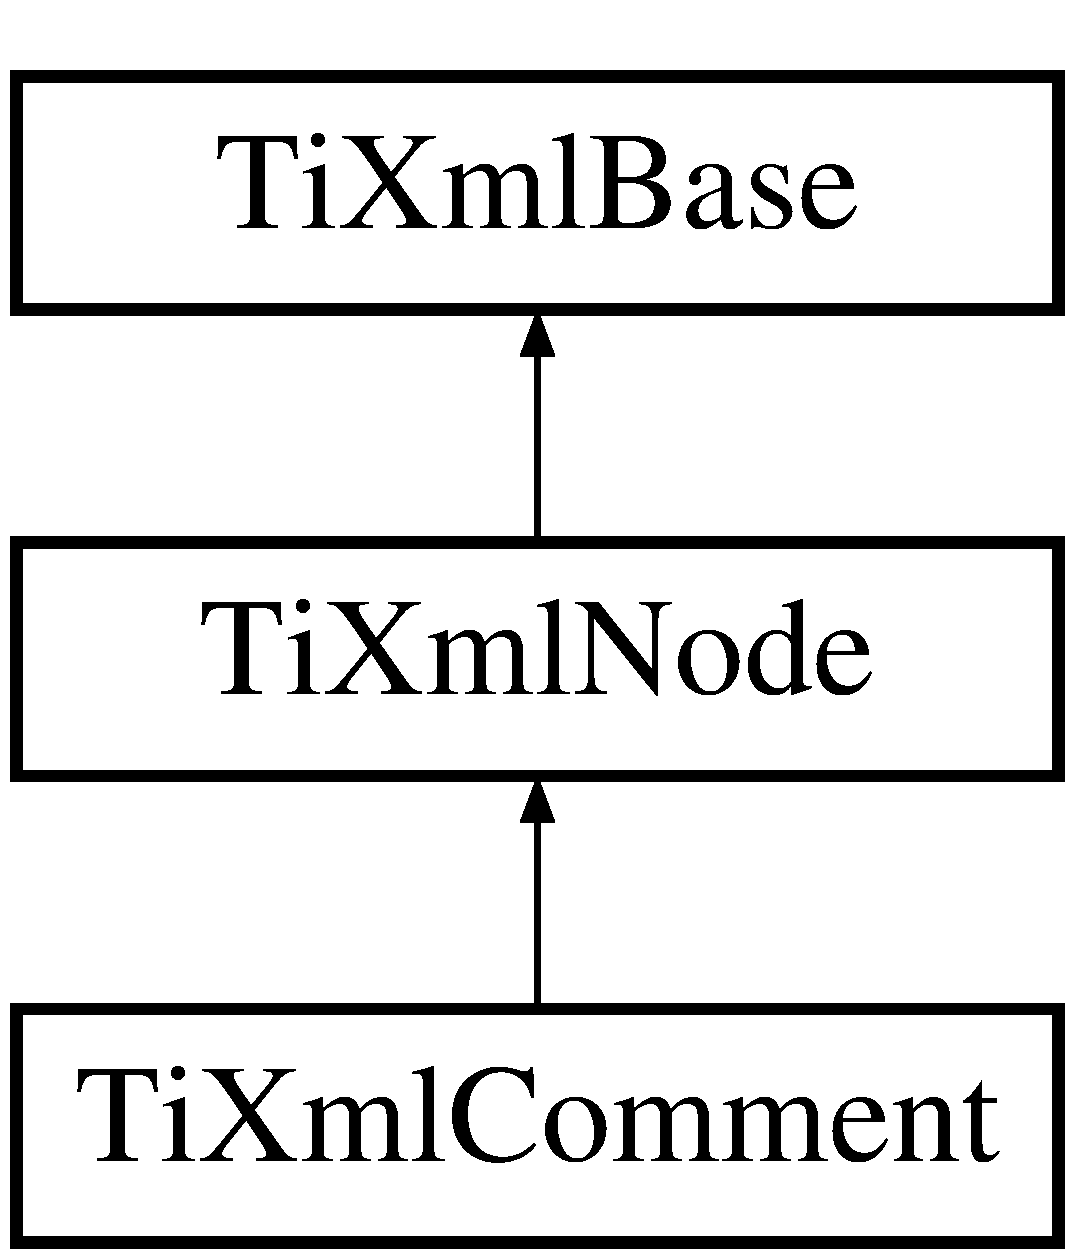
\includegraphics[height=3.000000cm]{classTiXmlComment}
\end{center}
\end{figure}
\subsection*{Public Member Functions}
\begin{DoxyCompactItemize}
\item 
\mbox{\label{classTiXmlComment_aaa3252031d3e8bd3a2bf51a1c61201b7}} 
\textbf{ Ti\+Xml\+Comment} ()
\begin{DoxyCompactList}\small\item\em Constructs an empty comment. \end{DoxyCompactList}\item 
\mbox{\label{classTiXmlComment_a37e7802ef17bc03ebe5ae79bf0713d47}} 
\textbf{ Ti\+Xml\+Comment} (const char $\ast$\+\_\+value)
\begin{DoxyCompactList}\small\item\em Construct a comment from text. \end{DoxyCompactList}\item 
\mbox{\label{classTiXmlComment_afaec41ac2760ce946ba1590eb5708e50}} 
{\bfseries Ti\+Xml\+Comment} (const \textbf{ Ti\+Xml\+Comment} \&)
\item 
\mbox{\label{classTiXmlComment_a46373f99b65cb960637dccb1f126bd49}} 
void {\bfseries operator=} (const \textbf{ Ti\+Xml\+Comment} \&base)
\item 
\mbox{\label{classTiXmlComment_a1f9f06e2ed3f77875093436193b16c16}} 
virtual \textbf{ Ti\+Xml\+Node} $\ast$ \textbf{ Clone} () const
\begin{DoxyCompactList}\small\item\em Returns a copy of this Comment. \end{DoxyCompactList}\item 
virtual void \textbf{ Print} (F\+I\+LE $\ast$cfile, int depth) const
\begin{DoxyCompactList}\small\item\em All Tiny\+Xml classes can print themselves to a filestream or the string class (\doxyref{Ti\+Xml\+String}{p.}{classTiXmlString} in non-\/\+S\+TL mode, std\+::string in S\+TL mode.) Either or both cfile and str can be null. \end{DoxyCompactList}\item 
\mbox{\label{classTiXmlComment_a43bddc18ac057734b41d84653b71d3e0}} 
virtual const char $\ast$ {\bfseries Parse} (const char $\ast$p, \textbf{ Ti\+Xml\+Parsing\+Data} $\ast$data, Ti\+Xml\+Encoding encoding)
\item 
\mbox{\label{classTiXmlComment_a1032e176d3eb73017ceabc698cac0f16}} 
virtual const \textbf{ Ti\+Xml\+Comment} $\ast$ \textbf{ To\+Comment} () const
\begin{DoxyCompactList}\small\item\em Cast to a more defined type. Will return null not of the requested type. \end{DoxyCompactList}\item 
\mbox{\label{classTiXmlComment_acc7c7e07e13c23f17797d642981511df}} 
virtual \textbf{ Ti\+Xml\+Comment} $\ast$ \textbf{ To\+Comment} ()
\begin{DoxyCompactList}\small\item\em Cast to a more defined type. Will return null not of the requested type. \end{DoxyCompactList}\item 
\mbox{\label{classTiXmlComment_ac894241530d1d266131a5026cb251a95}} 
virtual bool \textbf{ Accept} (\textbf{ Ti\+Xml\+Visitor} $\ast$visitor) const
\begin{DoxyCompactList}\small\item\em Walk the X\+ML tree visiting this node and all of its children. \end{DoxyCompactList}\end{DoxyCompactItemize}
\subsection*{Protected Member Functions}
\begin{DoxyCompactItemize}
\item 
\mbox{\label{classTiXmlComment_aaeb8a0b2d503f603879a2d04ceb54295}} 
void {\bfseries Copy\+To} (\textbf{ Ti\+Xml\+Comment} $\ast$target) const
\item 
\mbox{\label{classTiXmlComment_ad69c1024082f716462b6fd4b94488320}} 
virtual void {\bfseries Stream\+In} (std\+::istream $\ast$in, T\+I\+X\+M\+L\+\_\+\+S\+T\+R\+I\+NG $\ast$tag)
\end{DoxyCompactItemize}
\subsection*{Additional Inherited Members}


\subsection{Detailed Description}
An X\+ML comment. 

\subsection{Member Function Documentation}
\mbox{\label{classTiXmlComment_a873171beac19d40f0eaae945711c98ed}} 
\index{Ti\+Xml\+Comment@{Ti\+Xml\+Comment}!Print@{Print}}
\index{Print@{Print}!Ti\+Xml\+Comment@{Ti\+Xml\+Comment}}
\subsubsection{Print()}
{\footnotesize\ttfamily void Ti\+Xml\+Comment\+::\+Print (\begin{DoxyParamCaption}\item[{F\+I\+LE $\ast$}]{cfile,  }\item[{int}]{depth }\end{DoxyParamCaption}) const\hspace{0.3cm}{\ttfamily [virtual]}}



All Tiny\+Xml classes can print themselves to a filestream or the string class (\doxyref{Ti\+Xml\+String}{p.}{classTiXmlString} in non-\/\+S\+TL mode, std\+::string in S\+TL mode.) Either or both cfile and str can be null. 

This is a formatted print, and will insert tabs and newlines.

(For an unformatted stream, use the $<$$<$ operator.) 

Implements \textbf{ Ti\+Xml\+Base} \doxyref{}{p.}{classTiXmlBase_a0de56b3f2ef14c65091a3b916437b512}.



The documentation for this class was generated from the following files\+:\begin{DoxyCompactItemize}
\item 
tinyxml.\+h\item 
tinyxml.\+cc\item 
tinyxmlparser.\+cc\end{DoxyCompactItemize}

\section{Ti\+Xml\+Cursor Struct Reference}
\label{structTiXmlCursor}\index{Ti\+Xml\+Cursor@{Ti\+Xml\+Cursor}}
\subsection*{Public Member Functions}
\begin{DoxyCompactItemize}
\item 
\mbox{\label{structTiXmlCursor_a1e6fa622b59dafb71b6efe595105dcdd}} 
void {\bfseries Clear} ()
\end{DoxyCompactItemize}
\subsection*{Public Attributes}
\begin{DoxyCompactItemize}
\item 
\mbox{\label{structTiXmlCursor_a5b54dd949820c2db061e2be41f3effb3}} 
int {\bfseries row}
\item 
\mbox{\label{structTiXmlCursor_a5694d7ed2c4d20109d350c14c417969d}} 
int {\bfseries col}
\end{DoxyCompactItemize}


The documentation for this struct was generated from the following file\+:\begin{DoxyCompactItemize}
\item 
tinyxml.\+h\end{DoxyCompactItemize}

\section{Ti\+Xml\+Declaration Class Reference}
\label{classTiXmlDeclaration}\index{Ti\+Xml\+Declaration@{Ti\+Xml\+Declaration}}


In correct X\+ML the declaration is the first entry in the file.  




{\ttfamily \#include $<$tinyxml.\+h$>$}

Inheritance diagram for Ti\+Xml\+Declaration\+:\begin{figure}[H]
\begin{center}
\leavevmode
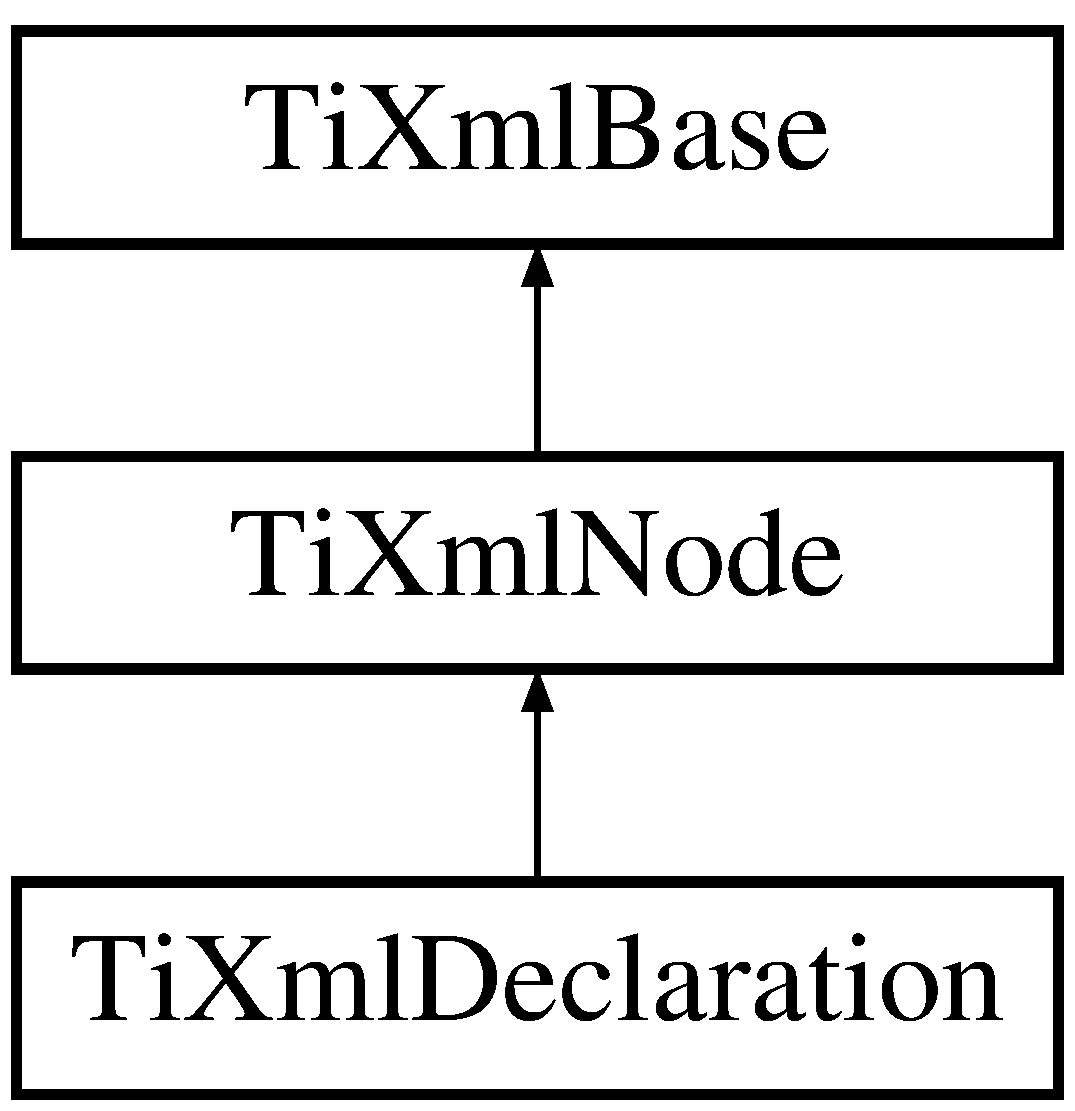
\includegraphics[height=3.000000cm]{classTiXmlDeclaration}
\end{center}
\end{figure}
\subsection*{Public Member Functions}
\begin{DoxyCompactItemize}
\item 
\mbox{\label{classTiXmlDeclaration_aa0484d059bea0ea1acb47c9094382d79}} 
\textbf{ Ti\+Xml\+Declaration} ()
\begin{DoxyCompactList}\small\item\em Construct an empty declaration. \end{DoxyCompactList}\item 
\mbox{\label{classTiXmlDeclaration_acd5556007c3c72209465081de39d9836}} 
\textbf{ Ti\+Xml\+Declaration} (const std\+::string \&\+\_\+version, const std\+::string \&\+\_\+encoding, const std\+::string \&\+\_\+standalone)
\begin{DoxyCompactList}\small\item\em Constructor. \end{DoxyCompactList}\item 
\mbox{\label{classTiXmlDeclaration_a3b618d1c30c25e4b7a71f31a595ee298}} 
\textbf{ Ti\+Xml\+Declaration} (const char $\ast$\+\_\+version, const char $\ast$\+\_\+encoding, const char $\ast$\+\_\+standalone)
\begin{DoxyCompactList}\small\item\em Construct. \end{DoxyCompactList}\item 
\mbox{\label{classTiXmlDeclaration_a58ac9042c342f7845c8491da0bb091e8}} 
{\bfseries Ti\+Xml\+Declaration} (const \textbf{ Ti\+Xml\+Declaration} \&copy)
\item 
\mbox{\label{classTiXmlDeclaration_a0fedc57539af9049be8db2d7d9d9ba33}} 
void {\bfseries operator=} (const \textbf{ Ti\+Xml\+Declaration} \&copy)
\item 
\mbox{\label{classTiXmlDeclaration_a95cdcb9354ea220065bd378ffcacc7bd}} 
const char $\ast$ \textbf{ Version} () const
\begin{DoxyCompactList}\small\item\em Version. Will return an empty string if none was found. \end{DoxyCompactList}\item 
\mbox{\label{classTiXmlDeclaration_a8d3d1b5b226daa8353276d719497be80}} 
const char $\ast$ \textbf{ Encoding} () const
\begin{DoxyCompactList}\small\item\em Encoding. Will return an empty string if none was found. \end{DoxyCompactList}\item 
\mbox{\label{classTiXmlDeclaration_a1f2f8a741593d15a61e491e5024cacef}} 
const char $\ast$ \textbf{ Standalone} () const
\begin{DoxyCompactList}\small\item\em Is this a standalone document? \end{DoxyCompactList}\item 
\mbox{\label{classTiXmlDeclaration_a35dc1455f69b79e81cae28e186944610}} 
virtual \textbf{ Ti\+Xml\+Node} $\ast$ \textbf{ Clone} () const
\begin{DoxyCompactList}\small\item\em Creates a copy of this Declaration and returns it. \end{DoxyCompactList}\item 
\mbox{\label{classTiXmlDeclaration_ace687d02a5a25a060ae3802abb1b3f55}} 
virtual void {\bfseries Print} (F\+I\+LE $\ast$cfile, int depth, T\+I\+X\+M\+L\+\_\+\+S\+T\+R\+I\+NG $\ast$str) const
\item 
virtual void \textbf{ Print} (F\+I\+LE $\ast$cfile, int depth) const
\begin{DoxyCompactList}\small\item\em All Tiny\+Xml classes can print themselves to a filestream or the string class (\doxyref{Ti\+Xml\+String}{p.}{classTiXmlString} in non-\/\+S\+TL mode, std\+::string in S\+TL mode.) Either or both cfile and str can be null. \end{DoxyCompactList}\item 
\mbox{\label{classTiXmlDeclaration_a9839ea97ed687a2b7342fd7b0f04361b}} 
virtual const char $\ast$ {\bfseries Parse} (const char $\ast$p, \textbf{ Ti\+Xml\+Parsing\+Data} $\ast$data, Ti\+Xml\+Encoding encoding)
\item 
\mbox{\label{classTiXmlDeclaration_aab62703b620d9b9391b482dc1835ecf6}} 
virtual const \textbf{ Ti\+Xml\+Declaration} $\ast$ \textbf{ To\+Declaration} () const
\begin{DoxyCompactList}\small\item\em Cast to a more defined type. Will return null not of the requested type. \end{DoxyCompactList}\item 
\mbox{\label{classTiXmlDeclaration_a6bd3d1daddcaeb9543c24bfd090969ce}} 
virtual \textbf{ Ti\+Xml\+Declaration} $\ast$ \textbf{ To\+Declaration} ()
\begin{DoxyCompactList}\small\item\em Cast to a more defined type. Will return null not of the requested type. \end{DoxyCompactList}\item 
\mbox{\label{classTiXmlDeclaration_aa1b6bade6c989407ce9881bdfc73c1e6}} 
virtual bool \textbf{ Accept} (\textbf{ Ti\+Xml\+Visitor} $\ast$visitor) const
\begin{DoxyCompactList}\small\item\em Walk the X\+ML tree visiting this node and all of its children. \end{DoxyCompactList}\end{DoxyCompactItemize}
\subsection*{Protected Member Functions}
\begin{DoxyCompactItemize}
\item 
\mbox{\label{classTiXmlDeclaration_a189de17b3e04d4e5b1c385336f214af1}} 
void {\bfseries Copy\+To} (\textbf{ Ti\+Xml\+Declaration} $\ast$target) const
\item 
\mbox{\label{classTiXmlDeclaration_a72e455200e6b6e265e76bdec4417bb73}} 
virtual void {\bfseries Stream\+In} (std\+::istream $\ast$in, T\+I\+X\+M\+L\+\_\+\+S\+T\+R\+I\+NG $\ast$tag)
\end{DoxyCompactItemize}
\subsection*{Additional Inherited Members}


\subsection{Detailed Description}
In correct X\+ML the declaration is the first entry in the file. 

\begin{DoxyVerb}        <?xml version="1.0" standalone="yes"?>\end{DoxyVerb}


Tiny\+Xml will happily read or write files without a declaration, however. There are 3 possible attributes to the declaration\+: version, encoding, and standalone.

Note\+: In this version of the code, the attributes are handled as special cases, not generic attributes, simply because there can only be at most 3 and they are always the same. 

\subsection{Member Function Documentation}
\mbox{\label{classTiXmlDeclaration_ae46cff6565f299210ab945e78bf28514}} 
\index{Ti\+Xml\+Declaration@{Ti\+Xml\+Declaration}!Print@{Print}}
\index{Print@{Print}!Ti\+Xml\+Declaration@{Ti\+Xml\+Declaration}}
\subsubsection{Print()}
{\footnotesize\ttfamily virtual void Ti\+Xml\+Declaration\+::\+Print (\begin{DoxyParamCaption}\item[{F\+I\+LE $\ast$}]{cfile,  }\item[{int}]{depth }\end{DoxyParamCaption}) const\hspace{0.3cm}{\ttfamily [inline]}, {\ttfamily [virtual]}}



All Tiny\+Xml classes can print themselves to a filestream or the string class (\doxyref{Ti\+Xml\+String}{p.}{classTiXmlString} in non-\/\+S\+TL mode, std\+::string in S\+TL mode.) Either or both cfile and str can be null. 

This is a formatted print, and will insert tabs and newlines.

(For an unformatted stream, use the $<$$<$ operator.) 

Implements \textbf{ Ti\+Xml\+Base} \doxyref{}{p.}{classTiXmlBase_a0de56b3f2ef14c65091a3b916437b512}.



The documentation for this class was generated from the following files\+:\begin{DoxyCompactItemize}
\item 
tinyxml.\+h\item 
tinyxml.\+cc\item 
tinyxmlparser.\+cc\end{DoxyCompactItemize}

\section{Ti\+Xml\+Document Class Reference}
\label{classTiXmlDocument}\index{Ti\+Xml\+Document@{Ti\+Xml\+Document}}


Always the top level node.  




{\ttfamily \#include $<$tinyxml.\+h$>$}

Inheritance diagram for Ti\+Xml\+Document\+:\begin{figure}[H]
\begin{center}
\leavevmode
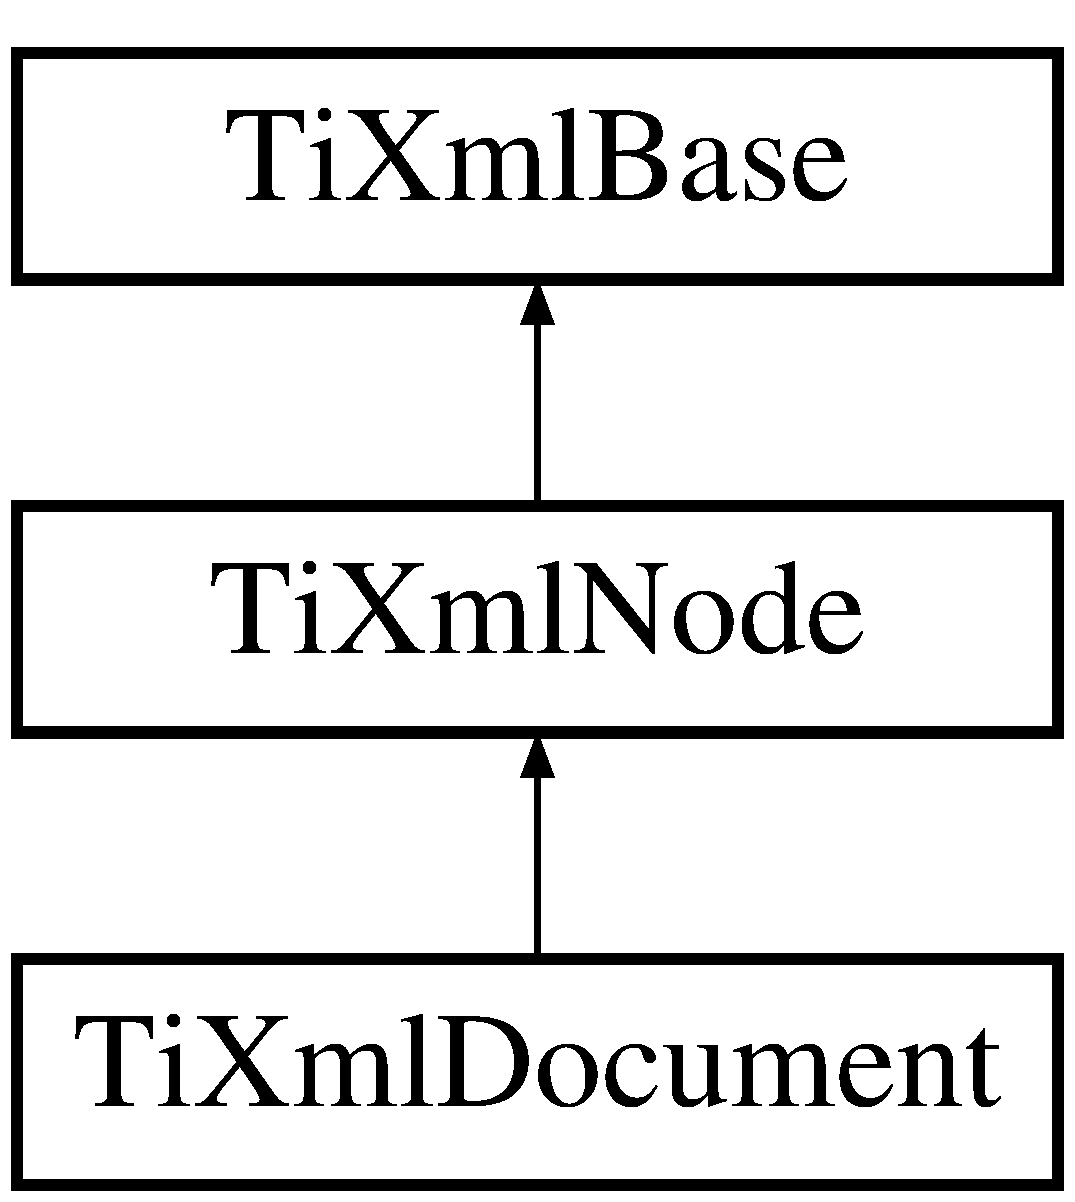
\includegraphics[height=3.000000cm]{classTiXmlDocument}
\end{center}
\end{figure}
\subsection*{Public Member Functions}
\begin{DoxyCompactItemize}
\item 
\mbox{\label{classTiXmlDocument_a9f5e84335708fde98400230f9f12659c}} 
\textbf{ Ti\+Xml\+Document} ()
\begin{DoxyCompactList}\small\item\em Create an empty document, that has no name. \end{DoxyCompactList}\item 
\mbox{\label{classTiXmlDocument_ae4508b452d0c3061db085f3db27b8396}} 
\textbf{ Ti\+Xml\+Document} (const char $\ast$document\+Name)
\begin{DoxyCompactList}\small\item\em Create a document with a name. The name of the document is also the filename of the xml. \end{DoxyCompactList}\item 
\mbox{\label{classTiXmlDocument_a2c6e58fb99bfa76cc613f16840022225}} 
\textbf{ Ti\+Xml\+Document} (const std\+::string \&document\+Name)
\begin{DoxyCompactList}\small\item\em Constructor. \end{DoxyCompactList}\item 
\mbox{\label{classTiXmlDocument_a323a7486e7da6099cdc19a5ff7e74b07}} 
{\bfseries Ti\+Xml\+Document} (const \textbf{ Ti\+Xml\+Document} \&copy)
\item 
\mbox{\label{classTiXmlDocument_aafbfacc3414008f619b1345775ef12a4}} 
void {\bfseries operator=} (const \textbf{ Ti\+Xml\+Document} \&copy)
\item 
bool \textbf{ Load\+File} (Ti\+Xml\+Encoding encoding=T\+I\+X\+M\+L\+\_\+\+D\+E\+F\+A\+U\+L\+T\+\_\+\+E\+N\+C\+O\+D\+I\+NG)
\begin{DoxyCompactList}\small\item\em Load a file using the current document value. \end{DoxyCompactList}\item 
\mbox{\label{classTiXmlDocument_ab63b96a6af5a467e289c7c75202edad9}} 
bool \textbf{ Save\+File} () const
\begin{DoxyCompactList}\small\item\em Save a file using the current document value. Returns true if successful. \end{DoxyCompactList}\item 
\mbox{\label{classTiXmlDocument_a879cdf5e981b8b2d2ef82f2546dd28fb}} 
bool \textbf{ Load\+File} (const char $\ast$filename, Ti\+Xml\+Encoding encoding=T\+I\+X\+M\+L\+\_\+\+D\+E\+F\+A\+U\+L\+T\+\_\+\+E\+N\+C\+O\+D\+I\+NG)
\begin{DoxyCompactList}\small\item\em Load a file using the given filename. Returns true if successful. \end{DoxyCompactList}\item 
\mbox{\label{classTiXmlDocument_ae641f33784381017c44e107cc2c86b5c}} 
bool \textbf{ Save\+File} (const char $\ast$filename) const
\begin{DoxyCompactList}\small\item\em Save a file using the given filename. Returns true if successful. \end{DoxyCompactList}\item 
bool \textbf{ Load\+File} (F\+I\+LE $\ast$, Ti\+Xml\+Encoding encoding=T\+I\+X\+M\+L\+\_\+\+D\+E\+F\+A\+U\+L\+T\+\_\+\+E\+N\+C\+O\+D\+I\+NG)
\begin{DoxyCompactList}\small\item\em Load a file using the given F\+I\+L\+E$\ast$. \end{DoxyCompactList}\item 
\mbox{\label{classTiXmlDocument_a8f5a1022168a5767e32becec7b6f44ee}} 
bool \textbf{ Save\+File} (F\+I\+LE $\ast$) const
\begin{DoxyCompactList}\small\item\em Save a file using the given F\+I\+L\+E$\ast$. Returns true if successful. \end{DoxyCompactList}\item 
bool \textbf{ Load\+File} (const std\+::string \&filename, Ti\+Xml\+Encoding encoding=T\+I\+X\+M\+L\+\_\+\+D\+E\+F\+A\+U\+L\+T\+\_\+\+E\+N\+C\+O\+D\+I\+NG)
\item 
\mbox{\label{classTiXmlDocument_a2b3d316ed658852876d4852cd39c42d8}} 
bool \textbf{ Save\+File} (const std\+::string \&filename) const
\begin{DoxyCompactList}\small\item\em $<$ S\+TL std\+::string version. \end{DoxyCompactList}\item 
virtual const char $\ast$ \textbf{ Parse} (const char $\ast$p, \textbf{ Ti\+Xml\+Parsing\+Data} $\ast$data=0, Ti\+Xml\+Encoding encoding=T\+I\+X\+M\+L\+\_\+\+D\+E\+F\+A\+U\+L\+T\+\_\+\+E\+N\+C\+O\+D\+I\+NG)
\begin{DoxyCompactList}\small\item\em Parse the given null terminated block of xml data. \end{DoxyCompactList}\item 
const \textbf{ Ti\+Xml\+Element} $\ast$ \textbf{ Root\+Element} () const
\begin{DoxyCompactList}\small\item\em Get the root element -- the only top level element -- of the document. \end{DoxyCompactList}\item 
\mbox{\label{classTiXmlDocument_a0b43e762a23f938b06651bc90b8a1013}} 
\textbf{ Ti\+Xml\+Element} $\ast$ {\bfseries Root\+Element} ()
\item 
bool \textbf{ Error} () const
\begin{DoxyCompactList}\small\item\em If an error occurs, Error will be set to true. \end{DoxyCompactList}\item 
\mbox{\label{classTiXmlDocument_aab511be262e84a003e3bb86f0215c8c2}} 
const char $\ast$ \textbf{ Error\+Desc} () const
\begin{DoxyCompactList}\small\item\em Contains a textual (english) description of the error if one occurs. \end{DoxyCompactList}\item 
int \textbf{ Error\+Id} () const
\begin{DoxyCompactList}\small\item\em Generally, you probably want the error string ( \doxyref{Error\+Desc()}{p.}{classTiXmlDocument_aab511be262e84a003e3bb86f0215c8c2} ). \end{DoxyCompactList}\item 
int \textbf{ Error\+Row} () const
\begin{DoxyCompactList}\small\item\em Returns the location (if known) of the error. \end{DoxyCompactList}\item 
\mbox{\label{classTiXmlDocument_adea69de889449a2587afb8ee043f43f5}} 
int \textbf{ Error\+Col} () const
\begin{DoxyCompactList}\small\item\em The column where the error occured. See \doxyref{Error\+Row()}{p.}{classTiXmlDocument_a062e5257128a7da31b0b2e38cd524600} \end{DoxyCompactList}\item 
void \textbf{ Set\+Tab\+Size} (int \+\_\+tabsize)
\begin{DoxyCompactList}\small\item\em \doxyref{Set\+Tab\+Size()}{p.}{classTiXmlDocument_a51dac56316f89b35bdb7d0d433ba988e} allows the error reporting functions (\doxyref{Error\+Row()}{p.}{classTiXmlDocument_a062e5257128a7da31b0b2e38cd524600} and \doxyref{Error\+Col()}{p.}{classTiXmlDocument_adea69de889449a2587afb8ee043f43f5}) to report the correct values for row and column. \end{DoxyCompactList}\item 
\mbox{\label{classTiXmlDocument_a81e6ffeee8f5d025a171eabf79abdad7}} 
int {\bfseries Tab\+Size} () const
\item 
void \textbf{ Clear\+Error} ()
\begin{DoxyCompactList}\small\item\em If you have handled the error, it can be reset with this call. \end{DoxyCompactList}\item 
void \textbf{ Print} () const
\begin{DoxyCompactList}\small\item\em Write the document to standard out using formatted printing (\char`\"{}pretty print\char`\"{}). \end{DoxyCompactList}\item 
\mbox{\label{classTiXmlDocument_aa9e166fae51da603641380a964f21eeb}} 
virtual void \textbf{ Print} (F\+I\+LE $\ast$cfile, int depth=0) const
\begin{DoxyCompactList}\small\item\em Print this Document to a F\+I\+LE stream. \end{DoxyCompactList}\item 
\mbox{\label{classTiXmlDocument_a735c23e318597b920c94eae77fa206de}} 
void {\bfseries Set\+Error} (int err, const char $\ast$error\+Location, \textbf{ Ti\+Xml\+Parsing\+Data} $\ast$prev\+Data, Ti\+Xml\+Encoding encoding)
\item 
\mbox{\label{classTiXmlDocument_a468e582640e3c4f740f7168d8b4a6e4a}} 
virtual const \textbf{ Ti\+Xml\+Document} $\ast$ \textbf{ To\+Document} () const
\begin{DoxyCompactList}\small\item\em Cast to a more defined type. Will return null not of the requested type. \end{DoxyCompactList}\item 
\mbox{\label{classTiXmlDocument_a1025d942a1f328fd742d545e37efdd42}} 
virtual \textbf{ Ti\+Xml\+Document} $\ast$ \textbf{ To\+Document} ()
\begin{DoxyCompactList}\small\item\em Cast to a more defined type. Will return null not of the requested type. \end{DoxyCompactList}\item 
\mbox{\label{classTiXmlDocument_a8ddd6eec722cbd25900bbac664909bac}} 
virtual bool \textbf{ Accept} (\textbf{ Ti\+Xml\+Visitor} $\ast$content) const
\begin{DoxyCompactList}\small\item\em Walk the X\+ML tree visiting this node and all of its children. \end{DoxyCompactList}\end{DoxyCompactItemize}
\subsection*{Protected Member Functions}
\begin{DoxyCompactItemize}
\item 
virtual \textbf{ Ti\+Xml\+Node} $\ast$ \textbf{ Clone} () const
\begin{DoxyCompactList}\small\item\em Create an exact duplicate of this node and return it. \end{DoxyCompactList}\item 
\mbox{\label{classTiXmlDocument_ab6d70b2c19e46aedb9903b3c3aa2a568}} 
virtual void {\bfseries Stream\+In} (std\+::istream $\ast$in, T\+I\+X\+M\+L\+\_\+\+S\+T\+R\+I\+NG $\ast$tag)
\end{DoxyCompactItemize}
\subsection*{Additional Inherited Members}


\subsection{Detailed Description}
Always the top level node. 

A document binds together all the X\+ML pieces. It can be saved, loaded, and printed to the screen. The \textquotesingle{}value\textquotesingle{} of a document node is the xml file name. 

\subsection{Member Function Documentation}
\mbox{\label{classTiXmlDocument_ac66b8c28db86363315712a3574e87c35}} 
\index{Ti\+Xml\+Document@{Ti\+Xml\+Document}!Clear\+Error@{Clear\+Error}}
\index{Clear\+Error@{Clear\+Error}!Ti\+Xml\+Document@{Ti\+Xml\+Document}}
\subsubsection{Clear\+Error()}
{\footnotesize\ttfamily void Ti\+Xml\+Document\+::\+Clear\+Error (\begin{DoxyParamCaption}{ }\end{DoxyParamCaption})\hspace{0.3cm}{\ttfamily [inline]}}



If you have handled the error, it can be reset with this call. 

The error state is automatically cleared if you Parse a new X\+ML block. 

Referenced by Parse(), and Ti\+Xml\+Document().

\mbox{\label{classTiXmlDocument_a46a4dda6c56eb106d46d4046ae1e5353}} 
\index{Ti\+Xml\+Document@{Ti\+Xml\+Document}!Clone@{Clone}}
\index{Clone@{Clone}!Ti\+Xml\+Document@{Ti\+Xml\+Document}}
\subsubsection{Clone()}
{\footnotesize\ttfamily \textbf{ Ti\+Xml\+Node} $\ast$ Ti\+Xml\+Document\+::\+Clone (\begin{DoxyParamCaption}{ }\end{DoxyParamCaption}) const\hspace{0.3cm}{\ttfamily [protected]}, {\ttfamily [virtual]}}



Create an exact duplicate of this node and return it. 

The memory must be deleted by the caller. 

Implements \textbf{ Ti\+Xml\+Node} \doxyref{}{p.}{classTiXmlNode_a4508cc3a2d7a98e96a54cc09c37a78a4}.



References Ti\+Xml\+Document().

\mbox{\label{classTiXmlDocument_a348e68faad4a3498f413c51ee9bc321a}} 
\index{Ti\+Xml\+Document@{Ti\+Xml\+Document}!Error@{Error}}
\index{Error@{Error}!Ti\+Xml\+Document@{Ti\+Xml\+Document}}
\subsubsection{Error()}
{\footnotesize\ttfamily bool Ti\+Xml\+Document\+::\+Error (\begin{DoxyParamCaption}{ }\end{DoxyParamCaption}) const\hspace{0.3cm}{\ttfamily [inline]}}



If an error occurs, Error will be set to true. 

Also,
\begin{DoxyItemize}
\item The \doxyref{Error\+Id()}{p.}{classTiXmlDocument_abd928b49a646c8ed53e0453c555d96a2} will contain the integer identifier of the error (not generally useful)
\item The \doxyref{Error\+Desc()}{p.}{classTiXmlDocument_aab511be262e84a003e3bb86f0215c8c2} method will return the name of the error. (very useful)
\item The \doxyref{Error\+Row()}{p.}{classTiXmlDocument_a062e5257128a7da31b0b2e38cd524600} and \doxyref{Error\+Col()}{p.}{classTiXmlDocument_adea69de889449a2587afb8ee043f43f5} will return the location of the error (if known) 
\end{DoxyItemize}

Referenced by Load\+File().

\mbox{\label{classTiXmlDocument_abd928b49a646c8ed53e0453c555d96a2}} 
\index{Ti\+Xml\+Document@{Ti\+Xml\+Document}!Error\+Id@{Error\+Id}}
\index{Error\+Id@{Error\+Id}!Ti\+Xml\+Document@{Ti\+Xml\+Document}}
\subsubsection{Error\+Id()}
{\footnotesize\ttfamily int Ti\+Xml\+Document\+::\+Error\+Id (\begin{DoxyParamCaption}{ }\end{DoxyParamCaption}) const\hspace{0.3cm}{\ttfamily [inline]}}



Generally, you probably want the error string ( \doxyref{Error\+Desc()}{p.}{classTiXmlDocument_aab511be262e84a003e3bb86f0215c8c2} ). 

But if you prefer the Error\+Id, this function will fetch it. \mbox{\label{classTiXmlDocument_a062e5257128a7da31b0b2e38cd524600}} 
\index{Ti\+Xml\+Document@{Ti\+Xml\+Document}!Error\+Row@{Error\+Row}}
\index{Error\+Row@{Error\+Row}!Ti\+Xml\+Document@{Ti\+Xml\+Document}}
\subsubsection{Error\+Row()}
{\footnotesize\ttfamily int Ti\+Xml\+Document\+::\+Error\+Row (\begin{DoxyParamCaption}{ }\end{DoxyParamCaption}) const\hspace{0.3cm}{\ttfamily [inline]}}



Returns the location (if known) of the error. 

The first column is column 1, and the first row is row 1. A value of 0 means the row and column wasn\textquotesingle{}t applicable (memory errors, for example, have no row/column) or the parser lost the error. (An error in the error reporting, in that case.)

\begin{DoxySeeAlso}{See also}
\doxyref{Set\+Tab\+Size}{p.}{classTiXmlDocument_a51dac56316f89b35bdb7d0d433ba988e}, \doxyref{Row}{p.}{classTiXmlBase_ad0cacca5d76d156b26511f46080b442e}, \doxyref{Column}{p.}{classTiXmlBase_ad283b95d9858d5d78c334f4a61b07bb4} 
\end{DoxySeeAlso}


Referenced by marlin\+::\+X\+M\+L\+Parser\+::process\+Include\+Elements().

\mbox{\label{classTiXmlDocument_a4c852a889c02cf251117fd1d9fe1845f}} 
\index{Ti\+Xml\+Document@{Ti\+Xml\+Document}!Load\+File@{Load\+File}}
\index{Load\+File@{Load\+File}!Ti\+Xml\+Document@{Ti\+Xml\+Document}}
\subsubsection{Load\+File()\hspace{0.1cm}{\footnotesize\ttfamily [1/3]}}
{\footnotesize\ttfamily bool Ti\+Xml\+Document\+::\+Load\+File (\begin{DoxyParamCaption}\item[{Ti\+Xml\+Encoding}]{encoding = {\ttfamily TIXML\+\_\+DEFAULT\+\_\+ENCODING} }\end{DoxyParamCaption})}



Load a file using the current document value. 

Returns true if successful. Will delete any existing document data before loading. 

References Ti\+Xml\+Node\+::\+Value().



Referenced by Load\+File(), and marlin\+::\+X\+M\+L\+Parser\+::process\+Include\+Elements().

\mbox{\label{classTiXmlDocument_a41f6fe7200864d1dca663d230caf8db6}} 
\index{Ti\+Xml\+Document@{Ti\+Xml\+Document}!Load\+File@{Load\+File}}
\index{Load\+File@{Load\+File}!Ti\+Xml\+Document@{Ti\+Xml\+Document}}
\subsubsection{Load\+File()\hspace{0.1cm}{\footnotesize\ttfamily [2/3]}}
{\footnotesize\ttfamily bool Ti\+Xml\+Document\+::\+Load\+File (\begin{DoxyParamCaption}\item[{F\+I\+LE $\ast$}]{file,  }\item[{Ti\+Xml\+Encoding}]{encoding = {\ttfamily TIXML\+\_\+DEFAULT\+\_\+ENCODING} }\end{DoxyParamCaption})}



Load a file using the given F\+I\+L\+E$\ast$. 

Returns true if successful. Note that this method doesn\textquotesingle{}t stream -\/ the entire object pointed at by the F\+I\+L\+E$\ast$ will be interpreted as an X\+ML file. Tiny\+X\+ML doesn\textquotesingle{}t stream in X\+ML from the current file location. Streaming may be added in the future. 

References Ti\+Xml\+Node\+::\+Clear(), Error(), and Parse().

\mbox{\label{classTiXmlDocument_a18ae6ed34fed7991ebc220862dfac884}} 
\index{Ti\+Xml\+Document@{Ti\+Xml\+Document}!Load\+File@{Load\+File}}
\index{Load\+File@{Load\+File}!Ti\+Xml\+Document@{Ti\+Xml\+Document}}
\subsubsection{Load\+File()\hspace{0.1cm}{\footnotesize\ttfamily [3/3]}}
{\footnotesize\ttfamily bool Ti\+Xml\+Document\+::\+Load\+File (\begin{DoxyParamCaption}\item[{const std\+::string \&}]{filename,  }\item[{Ti\+Xml\+Encoding}]{encoding = {\ttfamily TIXML\+\_\+DEFAULT\+\_\+ENCODING} }\end{DoxyParamCaption})\hspace{0.3cm}{\ttfamily [inline]}}


\begin{DoxyParams}{Parameters}
{\em encoding} & S\+TL std\+::string version. \\
\hline
\end{DoxyParams}
\mbox{\label{classTiXmlDocument_a789ad2f06f93d52bdb5570b2f3670289}} 
\index{Ti\+Xml\+Document@{Ti\+Xml\+Document}!Parse@{Parse}}
\index{Parse@{Parse}!Ti\+Xml\+Document@{Ti\+Xml\+Document}}
\subsubsection{Parse()}
{\footnotesize\ttfamily const char $\ast$ Ti\+Xml\+Document\+::\+Parse (\begin{DoxyParamCaption}\item[{const char $\ast$}]{p,  }\item[{\textbf{ Ti\+Xml\+Parsing\+Data} $\ast$}]{data = {\ttfamily 0},  }\item[{Ti\+Xml\+Encoding}]{encoding = {\ttfamily TIXML\+\_\+DEFAULT\+\_\+ENCODING} }\end{DoxyParamCaption})\hspace{0.3cm}{\ttfamily [virtual]}}



Parse the given null terminated block of xml data. 

Passing in an encoding to this method (either T\+I\+X\+M\+L\+\_\+\+E\+N\+C\+O\+D\+I\+N\+G\+\_\+\+L\+E\+G\+A\+CY or T\+I\+X\+M\+L\+\_\+\+E\+N\+C\+O\+D\+I\+N\+G\+\_\+\+U\+T\+F8 will force Tiny\+Xml to use that encoding, regardless of what Tiny\+Xml might otherwise try to detect. 

Implements \textbf{ Ti\+Xml\+Base} \doxyref{}{p.}{classTiXmlBase}.



References Clear\+Error(), Ti\+Xml\+Declaration\+::\+Encoding(), Ti\+Xml\+Node\+::\+Get\+Document(), Ti\+Xml\+Base\+::\+Is\+White\+Space\+Condensed(), Ti\+Xml\+Node\+::\+Link\+End\+Child(), Ti\+Xml\+Attribute\+::\+Name(), Ti\+Xml\+Text\+::\+Set\+C\+D\+A\+T\+A(), Ti\+Xml\+Attribute\+::\+Set\+Value(), Ti\+Xml\+Node\+::\+To\+Declaration(), and Ti\+Xml\+Attribute\+::\+Value().



Referenced by Ti\+Xml\+Base\+::\+Get\+User\+Data(), and Load\+File().

\mbox{\label{classTiXmlDocument_aa4e8c1498a76dcde7191c683e1220882}} 
\index{Ti\+Xml\+Document@{Ti\+Xml\+Document}!Print@{Print}}
\index{Print@{Print}!Ti\+Xml\+Document@{Ti\+Xml\+Document}}
\subsubsection{Print()}
{\footnotesize\ttfamily void Ti\+Xml\+Document\+::\+Print (\begin{DoxyParamCaption}{ }\end{DoxyParamCaption}) const\hspace{0.3cm}{\ttfamily [inline]}}



Write the document to standard out using formatted printing (\char`\"{}pretty print\char`\"{}). 



References Print().



Referenced by Print(), and Save\+File().

\mbox{\label{classTiXmlDocument_ab54e3a93279fcf0ac80f06ed9c52f04a}} 
\index{Ti\+Xml\+Document@{Ti\+Xml\+Document}!Root\+Element@{Root\+Element}}
\index{Root\+Element@{Root\+Element}!Ti\+Xml\+Document@{Ti\+Xml\+Document}}
\subsubsection{Root\+Element()}
{\footnotesize\ttfamily const \textbf{ Ti\+Xml\+Element}$\ast$ Ti\+Xml\+Document\+::\+Root\+Element (\begin{DoxyParamCaption}{ }\end{DoxyParamCaption}) const\hspace{0.3cm}{\ttfamily [inline]}}



Get the root element -- the only top level element -- of the document. 

In well formed X\+ML, there should only be one. Tiny\+Xml is tolerant of multiple elements at the document level. \mbox{\label{classTiXmlDocument_a51dac56316f89b35bdb7d0d433ba988e}} 
\index{Ti\+Xml\+Document@{Ti\+Xml\+Document}!Set\+Tab\+Size@{Set\+Tab\+Size}}
\index{Set\+Tab\+Size@{Set\+Tab\+Size}!Ti\+Xml\+Document@{Ti\+Xml\+Document}}
\subsubsection{Set\+Tab\+Size()}
{\footnotesize\ttfamily void Ti\+Xml\+Document\+::\+Set\+Tab\+Size (\begin{DoxyParamCaption}\item[{int}]{\+\_\+tabsize }\end{DoxyParamCaption})\hspace{0.3cm}{\ttfamily [inline]}}



\doxyref{Set\+Tab\+Size()}{p.}{classTiXmlDocument_a51dac56316f89b35bdb7d0d433ba988e} allows the error reporting functions (\doxyref{Error\+Row()}{p.}{classTiXmlDocument_a062e5257128a7da31b0b2e38cd524600} and \doxyref{Error\+Col()}{p.}{classTiXmlDocument_adea69de889449a2587afb8ee043f43f5}) to report the correct values for row and column. 

It does not change the output or input in any way.

By calling this method, with a tab size greater than 0, the row and column of each node and attribute is stored when the file is loaded. Very useful for tracking the D\+OM back in to the source file.

The tab size is required for calculating the location of nodes. If not set, the default of 4 is used. The tabsize is set per document. Setting the tabsize to 0 disables row/column tracking.

Note that row and column tracking is not supported when using operator$>$$>$.

The tab size needs to be enabled before the parse or load. Correct usage\+: \begin{DoxyVerb}    TiXmlDocument doc;
    doc.SetTabSize( 8 );
    doc.Load( "myfile.xml" );\end{DoxyVerb}


\begin{DoxySeeAlso}{See also}
\doxyref{Row}{p.}{classTiXmlBase_ad0cacca5d76d156b26511f46080b442e}, \doxyref{Column}{p.}{classTiXmlBase_ad283b95d9858d5d78c334f4a61b07bb4} 
\end{DoxySeeAlso}


The documentation for this class was generated from the following files\+:\begin{DoxyCompactItemize}
\item 
tinyxml.\+h\item 
tinyxml.\+cc\item 
tinyxmlparser.\+cc\end{DoxyCompactItemize}

\section{Ti\+Xml\+Element Class Reference}
\label{classTiXmlElement}\index{Ti\+Xml\+Element@{Ti\+Xml\+Element}}


The element is a container class.  




{\ttfamily \#include $<$tinyxml.\+h$>$}

Inheritance diagram for Ti\+Xml\+Element\+:\begin{figure}[H]
\begin{center}
\leavevmode
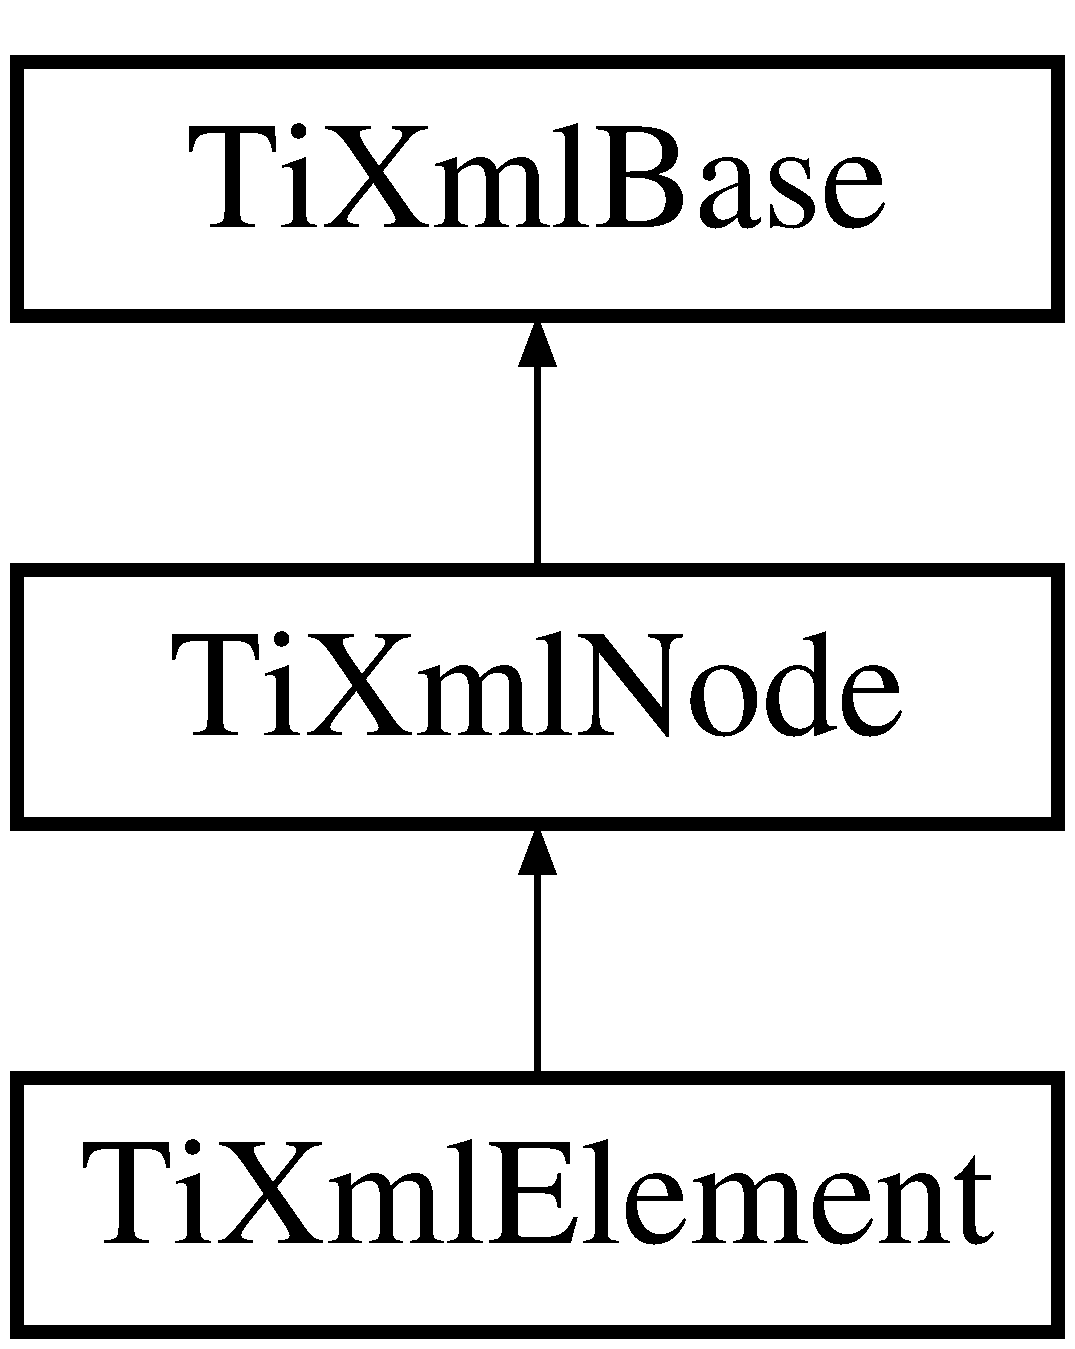
\includegraphics[height=3.000000cm]{classTiXmlElement}
\end{center}
\end{figure}
\subsection*{Public Member Functions}
\begin{DoxyCompactItemize}
\item 
\mbox{\label{classTiXmlElement_a01bc3ab372d35da08efcbbe65ad90c60}} 
\textbf{ Ti\+Xml\+Element} (const char $\ast$in\+\_\+value)
\begin{DoxyCompactList}\small\item\em Construct an element. \end{DoxyCompactList}\item 
\mbox{\label{classTiXmlElement_a40fc2e3c1a955e2f78e1a32350d180e7}} 
\textbf{ Ti\+Xml\+Element} (const std\+::string \&\+\_\+value)
\begin{DoxyCompactList}\small\item\em std\+::string constructor. \end{DoxyCompactList}\item 
\mbox{\label{classTiXmlElement_a1ca4465f3c2eac6a60e641cd7f1d9f7e}} 
{\bfseries Ti\+Xml\+Element} (const \textbf{ Ti\+Xml\+Element} \&)
\item 
\mbox{\label{classTiXmlElement_af5cd4156e082ef3bf23adfe0ed173340}} 
void {\bfseries operator=} (const \textbf{ Ti\+Xml\+Element} \&base)
\item 
\mbox{\label{classTiXmlElement_a6042f518748f475a7ac4b4e0b509eb05}} 
const char $\ast$ \textbf{ Attribute} (const char $\ast$name) const
\begin{DoxyCompactList}\small\item\em Given an attribute name, \doxyref{Attribute()}{p.}{classTiXmlElement_a6042f518748f475a7ac4b4e0b509eb05} returns the value for the attribute of that name, or null if none exists. \end{DoxyCompactList}\item 
const char $\ast$ \textbf{ Attribute} (const char $\ast$name, int $\ast$i) const
\begin{DoxyCompactList}\small\item\em Given an attribute name, \doxyref{Attribute()}{p.}{classTiXmlElement_a6042f518748f475a7ac4b4e0b509eb05} returns the value for the attribute of that name, or null if none exists. \end{DoxyCompactList}\item 
const char $\ast$ \textbf{ Attribute} (const char $\ast$name, double $\ast$d) const
\begin{DoxyCompactList}\small\item\em Given an attribute name, \doxyref{Attribute()}{p.}{classTiXmlElement_a6042f518748f475a7ac4b4e0b509eb05} returns the value for the attribute of that name, or null if none exists. \end{DoxyCompactList}\item 
int \textbf{ Query\+Int\+Attribute} (const char $\ast$name, int $\ast$\+\_\+value) const
\begin{DoxyCompactList}\small\item\em Query\+Int\+Attribute examines the attribute -\/ it is an alternative to the \doxyref{Attribute()}{p.}{classTiXmlElement_a6042f518748f475a7ac4b4e0b509eb05} method with richer error checking. \end{DoxyCompactList}\item 
\mbox{\label{classTiXmlElement_ae04bad29ddb281a7e6c662b3882e9928}} 
int \textbf{ Query\+Double\+Attribute} (const char $\ast$name, double $\ast$\+\_\+value) const
\begin{DoxyCompactList}\small\item\em Query\+Double\+Attribute examines the attribute -\/ see \doxyref{Query\+Int\+Attribute()}{p.}{classTiXmlElement_a5c0f739e0f6f5905a201364532e54a60}. \end{DoxyCompactList}\item 
\mbox{\label{classTiXmlElement_a5591929834178699b4561ab6ab460068}} 
int \textbf{ Query\+Float\+Attribute} (const char $\ast$name, float $\ast$\+\_\+value) const
\begin{DoxyCompactList}\small\item\em Query\+Float\+Attribute examines the attribute -\/ see \doxyref{Query\+Int\+Attribute()}{p.}{classTiXmlElement_a5c0f739e0f6f5905a201364532e54a60}. \end{DoxyCompactList}\item 
{\footnotesize template$<$typename T $>$ }\\int \textbf{ Query\+Value\+Attribute} (const std\+::string \&name, T $\ast$out\+Value) const
\begin{DoxyCompactList}\small\item\em Template form of the attribute query which will try to read the attribute into the specified type. \end{DoxyCompactList}\item 
void \textbf{ Set\+Attribute} (const char $\ast$name, const char $\ast$\+\_\+value)
\begin{DoxyCompactList}\small\item\em Sets an attribute of name to a given value. \end{DoxyCompactList}\item 
\mbox{\label{classTiXmlElement_a9c3d9bfacd95cf549fcd859238bb8f93}} 
const std\+::string $\ast$ {\bfseries Attribute} (const std\+::string \&name) const
\item 
\mbox{\label{classTiXmlElement_a51227b271c63c370eb3477b25a529606}} 
const std\+::string $\ast$ {\bfseries Attribute} (const std\+::string \&name, int $\ast$i) const
\item 
\mbox{\label{classTiXmlElement_abf7279768e400864271dc163258bb1e9}} 
const std\+::string $\ast$ {\bfseries Attribute} (const std\+::string \&name, double $\ast$d) const
\item 
\mbox{\label{classTiXmlElement_aa368685cfa6efae820b8e7ec18114865}} 
int {\bfseries Query\+Int\+Attribute} (const std\+::string \&name, int $\ast$\+\_\+value) const
\item 
\mbox{\label{classTiXmlElement_a442a0180263ff9a61d30711dc213d9e4}} 
int {\bfseries Query\+Double\+Attribute} (const std\+::string \&name, double $\ast$\+\_\+value) const
\item 
void \textbf{ Set\+Attribute} (const std\+::string \&name, const std\+::string \&\+\_\+value)
\begin{DoxyCompactList}\small\item\em S\+TL std\+::string form. \end{DoxyCompactList}\item 
\mbox{\label{classTiXmlElement_a6f18d54fbe25bbc527936ee65363b3c5}} 
void {\bfseries Set\+Attribute} (const std\+::string \&name, int \+\_\+value)
\item 
void \textbf{ Set\+Attribute} (const char $\ast$name, int value)
\begin{DoxyCompactList}\small\item\em Sets an attribute of name to a given value. \end{DoxyCompactList}\item 
void \textbf{ Set\+Double\+Attribute} (const char $\ast$name, double value)
\begin{DoxyCompactList}\small\item\em Sets an attribute of name to a given value. \end{DoxyCompactList}\item 
\mbox{\label{classTiXmlElement_a56979767deca794376b1dfa69a525b2a}} 
void \textbf{ Remove\+Attribute} (const char $\ast$name)
\begin{DoxyCompactList}\small\item\em Deletes an attribute with the given name. \end{DoxyCompactList}\item 
\mbox{\label{classTiXmlElement_a1afa6aea716511326a608e4c05df4f3a}} 
void \textbf{ Remove\+Attribute} (const std\+::string \&name)
\begin{DoxyCompactList}\small\item\em S\+TL std\+::string form. \end{DoxyCompactList}\item 
\mbox{\label{classTiXmlElement_a003131b1bbf0b8054b11571c1b9a4d3a}} 
const \textbf{ Ti\+Xml\+Attribute} $\ast$ \textbf{ First\+Attribute} () const
\begin{DoxyCompactList}\small\item\em Access the first attribute in this element. \end{DoxyCompactList}\item 
\mbox{\label{classTiXmlElement_a4b33780fc565d38d6b54f640e0cf1737}} 
\textbf{ Ti\+Xml\+Attribute} $\ast$ {\bfseries First\+Attribute} ()
\item 
\mbox{\label{classTiXmlElement_a42939f55ed4cec5fc1daaecfded7ba16}} 
const \textbf{ Ti\+Xml\+Attribute} $\ast$ \textbf{ Last\+Attribute} () const
\begin{DoxyCompactList}\small\item\em Access the last attribute in this element. \end{DoxyCompactList}\item 
\mbox{\label{classTiXmlElement_a222f81cf06155cd108f2a68d4d176004}} 
\textbf{ Ti\+Xml\+Attribute} $\ast$ {\bfseries Last\+Attribute} ()
\item 
const char $\ast$ \textbf{ Get\+Text} () const
\begin{DoxyCompactList}\small\item\em Convenience function for easy access to the text inside an element. \end{DoxyCompactList}\item 
\mbox{\label{classTiXmlElement_a810ea8fa40844c01334e5af2a26794cb}} 
virtual \textbf{ Ti\+Xml\+Node} $\ast$ \textbf{ Clone} () const
\begin{DoxyCompactList}\small\item\em Creates a new Element and returns it -\/ the returned element is a copy. \end{DoxyCompactList}\item 
virtual void \textbf{ Print} (F\+I\+LE $\ast$cfile, int depth) const
\begin{DoxyCompactList}\small\item\em All Tiny\+Xml classes can print themselves to a filestream or the string class (\doxyref{Ti\+Xml\+String}{p.}{classTiXmlString} in non-\/\+S\+TL mode, std\+::string in S\+TL mode.) Either or both cfile and str can be null. \end{DoxyCompactList}\item 
\mbox{\label{classTiXmlElement_af95c9165159fd9dfdcc5b894a3fcf85b}} 
virtual const char $\ast$ {\bfseries Parse} (const char $\ast$p, \textbf{ Ti\+Xml\+Parsing\+Data} $\ast$data, Ti\+Xml\+Encoding encoding)
\item 
\mbox{\label{classTiXmlElement_a940fc8aa953e0ef0de6e110b7d98b8ee}} 
virtual const \textbf{ Ti\+Xml\+Element} $\ast$ \textbf{ To\+Element} () const
\begin{DoxyCompactList}\small\item\em Cast to a more defined type. Will return null not of the requested type. \end{DoxyCompactList}\item 
\mbox{\label{classTiXmlElement_a9def86337ea7a755eb41cac980f60c7a}} 
virtual \textbf{ Ti\+Xml\+Element} $\ast$ \textbf{ To\+Element} ()
\begin{DoxyCompactList}\small\item\em Cast to a more defined type. Will return null not of the requested type. \end{DoxyCompactList}\item 
\mbox{\label{classTiXmlElement_a01d33358cce9d1817b557d314dda3779}} 
virtual bool \textbf{ Accept} (\textbf{ Ti\+Xml\+Visitor} $\ast$visitor) const
\begin{DoxyCompactList}\small\item\em Walk the X\+ML tree visiting this node and all of its children. \end{DoxyCompactList}\end{DoxyCompactItemize}
\subsection*{Protected Member Functions}
\begin{DoxyCompactItemize}
\item 
\mbox{\label{classTiXmlElement_ab931f2208ed76ba03465d8a1f86b5935}} 
void {\bfseries Copy\+To} (\textbf{ Ti\+Xml\+Element} $\ast$target) const
\item 
\mbox{\label{classTiXmlElement_a5670933ec2d7d9763b9891acc05d7f7d}} 
void {\bfseries Clear\+This} ()
\item 
\mbox{\label{classTiXmlElement_acc42052299e0bcf04871f3c2d229fe93}} 
virtual void {\bfseries Stream\+In} (std\+::istream $\ast$in, T\+I\+X\+M\+L\+\_\+\+S\+T\+R\+I\+NG $\ast$tag)
\item 
\mbox{\label{classTiXmlElement_ac786bce103042d3837c4cc2ff6967d41}} 
const char $\ast$ {\bfseries Read\+Value} (const char $\ast$in, \textbf{ Ti\+Xml\+Parsing\+Data} $\ast$prev\+Data, Ti\+Xml\+Encoding encoding)
\end{DoxyCompactItemize}
\subsection*{Additional Inherited Members}


\subsection{Detailed Description}
The element is a container class. 

It has a value, the element name, and can contain other elements, text, comments, and unknowns. Elements also contain an arbitrary number of attributes. 

\subsection{Member Function Documentation}
\mbox{\label{classTiXmlElement_a8005d0b808fd02bd1246710cdf95e5f6}} 
\index{Ti\+Xml\+Element@{Ti\+Xml\+Element}!Attribute@{Attribute}}
\index{Attribute@{Attribute}!Ti\+Xml\+Element@{Ti\+Xml\+Element}}
\subsubsection{Attribute()\hspace{0.1cm}{\footnotesize\ttfamily [1/2]}}
{\footnotesize\ttfamily const char $\ast$ Ti\+Xml\+Element\+::\+Attribute (\begin{DoxyParamCaption}\item[{const char $\ast$}]{name,  }\item[{int $\ast$}]{i }\end{DoxyParamCaption}) const}



Given an attribute name, \doxyref{Attribute()}{p.}{classTiXmlElement_a6042f518748f475a7ac4b4e0b509eb05} returns the value for the attribute of that name, or null if none exists. 

If the attribute exists and can be converted to an integer, the integer value will be put in the return \textquotesingle{}i\textquotesingle{}, if \textquotesingle{}i\textquotesingle{} is non-\/null. 

References Attribute().

\mbox{\label{classTiXmlElement_a09df893402d0ab1402c8725e6d30ec04}} 
\index{Ti\+Xml\+Element@{Ti\+Xml\+Element}!Attribute@{Attribute}}
\index{Attribute@{Attribute}!Ti\+Xml\+Element@{Ti\+Xml\+Element}}
\subsubsection{Attribute()\hspace{0.1cm}{\footnotesize\ttfamily [2/2]}}
{\footnotesize\ttfamily const char $\ast$ Ti\+Xml\+Element\+::\+Attribute (\begin{DoxyParamCaption}\item[{const char $\ast$}]{name,  }\item[{double $\ast$}]{d }\end{DoxyParamCaption}) const}



Given an attribute name, \doxyref{Attribute()}{p.}{classTiXmlElement_a6042f518748f475a7ac4b4e0b509eb05} returns the value for the attribute of that name, or null if none exists. 

If the attribute exists and can be converted to an double, the double value will be put in the return \textquotesingle{}d\textquotesingle{}, if \textquotesingle{}d\textquotesingle{} is non-\/null. 

References Attribute().

\mbox{\label{classTiXmlElement_af0f814ecbd43d50d4cdbdf4354d3da39}} 
\index{Ti\+Xml\+Element@{Ti\+Xml\+Element}!Get\+Text@{Get\+Text}}
\index{Get\+Text@{Get\+Text}!Ti\+Xml\+Element@{Ti\+Xml\+Element}}
\subsubsection{Get\+Text()}
{\footnotesize\ttfamily const char $\ast$ Ti\+Xml\+Element\+::\+Get\+Text (\begin{DoxyParamCaption}{ }\end{DoxyParamCaption}) const}



Convenience function for easy access to the text inside an element. 

Although easy and concise, \doxyref{Get\+Text()}{p.}{classTiXmlElement_af0f814ecbd43d50d4cdbdf4354d3da39} is limited compared to getting the \doxyref{Ti\+Xml\+Text}{p.}{classTiXmlText} child and accessing it directly.

If the first child of \textquotesingle{}this\textquotesingle{} is a \doxyref{Ti\+Xml\+Text}{p.}{classTiXmlText}, the \doxyref{Get\+Text()}{p.}{classTiXmlElement_af0f814ecbd43d50d4cdbdf4354d3da39} returns the character string of the Text node, else null is returned.

This is a convenient method for getting the text of simple contained text\+: \begin{DoxyVerb}    <foo>This is text</foo>
    const char* str = fooElement->GetText();\end{DoxyVerb}


\textquotesingle{}str\textquotesingle{} will be a pointer to \char`\"{}\+This is text\char`\"{}.

Note that this function can be misleading. If the element foo was created from this X\+ML\+: \begin{DoxyVerb}    <foo><b>This is text</b></foo> \end{DoxyVerb}


then the value of str would be null. The first child node isn\textquotesingle{}t a text node, it is another element. From this X\+ML\+: \begin{DoxyVerb}    <foo>This is <b>text</b></foo> \end{DoxyVerb}
 \doxyref{Get\+Text()}{p.}{classTiXmlElement_af0f814ecbd43d50d4cdbdf4354d3da39} will return \char`\"{}\+This is \char`\"{}.

W\+A\+R\+N\+I\+NG\+: \doxyref{Get\+Text()}{p.}{classTiXmlElement_af0f814ecbd43d50d4cdbdf4354d3da39} accesses a child node -\/ don\textquotesingle{}t become confused with the similarly named \doxyref{Ti\+Xml\+Handle\+::\+Text()}{p.}{classTiXmlHandle_ad3b502c72059421e4dfcc7bda3c392fe} and \doxyref{Ti\+Xml\+Node\+::\+To\+Text()}{p.}{classTiXmlNode_a3ddfbcac78fbea041fad57e5c6d60a03} which are safe type casts on the referenced node. 

References Ti\+Xml\+Node\+::\+First\+Child(), Ti\+Xml\+Node\+::\+To\+Text(), and Ti\+Xml\+Node\+::\+Value().

\mbox{\label{classTiXmlElement_aa31a15cddfb8601a31236fe7d2569fb4}} 
\index{Ti\+Xml\+Element@{Ti\+Xml\+Element}!Print@{Print}}
\index{Print@{Print}!Ti\+Xml\+Element@{Ti\+Xml\+Element}}
\subsubsection{Print()}
{\footnotesize\ttfamily void Ti\+Xml\+Element\+::\+Print (\begin{DoxyParamCaption}\item[{F\+I\+LE $\ast$}]{cfile,  }\item[{int}]{depth }\end{DoxyParamCaption}) const\hspace{0.3cm}{\ttfamily [virtual]}}



All Tiny\+Xml classes can print themselves to a filestream or the string class (\doxyref{Ti\+Xml\+String}{p.}{classTiXmlString} in non-\/\+S\+TL mode, std\+::string in S\+TL mode.) Either or both cfile and str can be null. 

This is a formatted print, and will insert tabs and newlines.

(For an unformatted stream, use the $<$$<$ operator.) 

Implements \textbf{ Ti\+Xml\+Base} \doxyref{}{p.}{classTiXmlBase_a0de56b3f2ef14c65091a3b916437b512}.



References Ti\+Xml\+Node\+::\+Clone(), Ti\+Xml\+Node\+::\+Link\+End\+Child(), Ti\+Xml\+Attribute\+::\+Name(), Ti\+Xml\+Attribute\+::\+Next(), Ti\+Xml\+Node\+::\+Next\+Sibling(), Ti\+Xml\+Base\+::\+Print(), Set\+Attribute(), Ti\+Xml\+Node\+::\+To\+Text(), and Ti\+Xml\+Attribute\+::\+Value().



Referenced by Ti\+Xml\+Text\+::\+Ti\+Xml\+Text().

\mbox{\label{classTiXmlElement_a5c0f739e0f6f5905a201364532e54a60}} 
\index{Ti\+Xml\+Element@{Ti\+Xml\+Element}!Query\+Int\+Attribute@{Query\+Int\+Attribute}}
\index{Query\+Int\+Attribute@{Query\+Int\+Attribute}!Ti\+Xml\+Element@{Ti\+Xml\+Element}}
\subsubsection{Query\+Int\+Attribute()}
{\footnotesize\ttfamily int Ti\+Xml\+Element\+::\+Query\+Int\+Attribute (\begin{DoxyParamCaption}\item[{const char $\ast$}]{name,  }\item[{int $\ast$}]{\+\_\+value }\end{DoxyParamCaption}) const}



Query\+Int\+Attribute examines the attribute -\/ it is an alternative to the \doxyref{Attribute()}{p.}{classTiXmlElement_a6042f518748f475a7ac4b4e0b509eb05} method with richer error checking. 

If the attribute is an integer, it is stored in \textquotesingle{}value\textquotesingle{} and the call returns T\+I\+X\+M\+L\+\_\+\+S\+U\+C\+C\+E\+SS. If it is not an integer, it returns T\+I\+X\+M\+L\+\_\+\+W\+R\+O\+N\+G\+\_\+\+T\+Y\+PE. If the attribute does not exist, then T\+I\+X\+M\+L\+\_\+\+N\+O\+\_\+\+A\+T\+T\+R\+I\+B\+U\+TE is returned. 

References Ti\+Xml\+Attribute\+::\+Query\+Int\+Value().

\mbox{\label{classTiXmlElement_a7530db879b81ebaba61bf62a9770d204}} 
\index{Ti\+Xml\+Element@{Ti\+Xml\+Element}!Query\+Value\+Attribute@{Query\+Value\+Attribute}}
\index{Query\+Value\+Attribute@{Query\+Value\+Attribute}!Ti\+Xml\+Element@{Ti\+Xml\+Element}}
\subsubsection{Query\+Value\+Attribute()}
{\footnotesize\ttfamily template$<$typename T $>$ \\
int Ti\+Xml\+Element\+::\+Query\+Value\+Attribute (\begin{DoxyParamCaption}\item[{const std\+::string \&}]{name,  }\item[{T $\ast$}]{out\+Value }\end{DoxyParamCaption}) const\hspace{0.3cm}{\ttfamily [inline]}}



Template form of the attribute query which will try to read the attribute into the specified type. 

Very easy, very powerful, but be careful to make sure to call this with the correct type.

\begin{DoxyReturn}{Returns}
T\+I\+X\+M\+L\+\_\+\+S\+U\+C\+C\+E\+SS, T\+I\+X\+M\+L\+\_\+\+W\+R\+O\+N\+G\+\_\+\+T\+Y\+PE, or T\+I\+X\+M\+L\+\_\+\+N\+O\+\_\+\+A\+T\+T\+R\+I\+B\+U\+TE 
\end{DoxyReturn}


References Ti\+Xml\+Attribute\+::\+Value\+Str().

\mbox{\label{classTiXmlElement_abf0b3bd7f0e4c746a89ec6e7f101fc32}} 
\index{Ti\+Xml\+Element@{Ti\+Xml\+Element}!Set\+Attribute@{Set\+Attribute}}
\index{Set\+Attribute@{Set\+Attribute}!Ti\+Xml\+Element@{Ti\+Xml\+Element}}
\subsubsection{Set\+Attribute()\hspace{0.1cm}{\footnotesize\ttfamily [1/3]}}
{\footnotesize\ttfamily void Ti\+Xml\+Element\+::\+Set\+Attribute (\begin{DoxyParamCaption}\item[{const char $\ast$}]{name,  }\item[{const char $\ast$}]{\+\_\+value }\end{DoxyParamCaption})}



Sets an attribute of name to a given value. 

The attribute will be created if it does not exist, or changed if it does. 

References Ti\+Xml\+Node\+::\+Get\+Document(), and Ti\+Xml\+Attribute\+::\+Set\+Value().



Referenced by marlin\+::\+X\+M\+L\+Parser\+::parameters\+From\+Node(), Print(), marlin\+::\+X\+M\+L\+Parser\+::processconditions(), marlin\+::\+X\+M\+L\+Parser\+::process\+Include\+Elements(), marlin\+::\+X\+M\+L\+Parser\+::replacegroups(), Set\+Attribute(), and Set\+Double\+Attribute().

\mbox{\label{classTiXmlElement_a80ed65b1d194c71c6c9986ae42337d7d}} 
\index{Ti\+Xml\+Element@{Ti\+Xml\+Element}!Set\+Attribute@{Set\+Attribute}}
\index{Set\+Attribute@{Set\+Attribute}!Ti\+Xml\+Element@{Ti\+Xml\+Element}}
\subsubsection{Set\+Attribute()\hspace{0.1cm}{\footnotesize\ttfamily [2/3]}}
{\footnotesize\ttfamily void Ti\+Xml\+Element\+::\+Set\+Attribute (\begin{DoxyParamCaption}\item[{const std\+::string \&}]{name,  }\item[{const std\+::string \&}]{\+\_\+value }\end{DoxyParamCaption})}



S\+TL std\+::string form. 

S\+TL std\+::string form. \mbox{\label{classTiXmlElement_ace6f4be75e373726d4774073d666d1a7}} 
\index{Ti\+Xml\+Element@{Ti\+Xml\+Element}!Set\+Attribute@{Set\+Attribute}}
\index{Set\+Attribute@{Set\+Attribute}!Ti\+Xml\+Element@{Ti\+Xml\+Element}}
\subsubsection{Set\+Attribute()\hspace{0.1cm}{\footnotesize\ttfamily [3/3]}}
{\footnotesize\ttfamily void Ti\+Xml\+Element\+::\+Set\+Attribute (\begin{DoxyParamCaption}\item[{const char $\ast$}]{name,  }\item[{int}]{value }\end{DoxyParamCaption})}



Sets an attribute of name to a given value. 

The attribute will be created if it does not exist, or changed if it does. 

References Set\+Attribute().

\mbox{\label{classTiXmlElement_a0d1dd975d75496778177e35abfe0ec0b}} 
\index{Ti\+Xml\+Element@{Ti\+Xml\+Element}!Set\+Double\+Attribute@{Set\+Double\+Attribute}}
\index{Set\+Double\+Attribute@{Set\+Double\+Attribute}!Ti\+Xml\+Element@{Ti\+Xml\+Element}}
\subsubsection{Set\+Double\+Attribute()}
{\footnotesize\ttfamily void Ti\+Xml\+Element\+::\+Set\+Double\+Attribute (\begin{DoxyParamCaption}\item[{const char $\ast$}]{name,  }\item[{double}]{value }\end{DoxyParamCaption})}



Sets an attribute of name to a given value. 

The attribute will be created if it does not exist, or changed if it does. 

References Set\+Attribute().



The documentation for this class was generated from the following files\+:\begin{DoxyCompactItemize}
\item 
tinyxml.\+h\item 
tinyxml.\+cc\item 
tinyxmlparser.\+cc\end{DoxyCompactItemize}

\section{Ti\+Xml\+Handle Class Reference}
\label{classTiXmlHandle}\index{Ti\+Xml\+Handle@{Ti\+Xml\+Handle}}


A \doxyref{Ti\+Xml\+Handle}{p.}{classTiXmlHandle} is a class that wraps a node pointer with null checks; this is an incredibly useful thing.  




{\ttfamily \#include $<$tinyxml.\+h$>$}

\subsection*{Public Member Functions}
\begin{DoxyCompactItemize}
\item 
\mbox{\label{classTiXmlHandle_aba18fd7bdefb942ecdea4bf4b8e29ec8}} 
\textbf{ Ti\+Xml\+Handle} (\textbf{ Ti\+Xml\+Node} $\ast$\+\_\+node)
\begin{DoxyCompactList}\small\item\em Create a handle from any node (at any depth of the tree.) This can be a null pointer. \end{DoxyCompactList}\item 
\mbox{\label{classTiXmlHandle_a236d7855e1e56ccc7b980630c48c7fd7}} 
\textbf{ Ti\+Xml\+Handle} (const \textbf{ Ti\+Xml\+Handle} \&ref)
\begin{DoxyCompactList}\small\item\em Copy constructor. \end{DoxyCompactList}\item 
\mbox{\label{classTiXmlHandle_ad8e5dcf6a87882674203157f29f8e4db}} 
\textbf{ Ti\+Xml\+Handle} {\bfseries operator=} (const \textbf{ Ti\+Xml\+Handle} \&ref)
\item 
\mbox{\label{classTiXmlHandle_afb1b4c0eda970b320dfd262304cc1d04}} 
\textbf{ Ti\+Xml\+Handle} \textbf{ First\+Child} () const
\begin{DoxyCompactList}\small\item\em Return a handle to the first child node. \end{DoxyCompactList}\item 
\mbox{\label{classTiXmlHandle_a586ebaca4a4d0909db65a765d95d5e59}} 
\textbf{ Ti\+Xml\+Handle} \textbf{ First\+Child} (const char $\ast$value) const
\begin{DoxyCompactList}\small\item\em Return a handle to the first child node with the given name. \end{DoxyCompactList}\item 
\mbox{\label{classTiXmlHandle_af0643f8683f3f2b779b8c9d78c67b2c0}} 
\textbf{ Ti\+Xml\+Handle} \textbf{ First\+Child\+Element} () const
\begin{DoxyCompactList}\small\item\em Return a handle to the first child element. \end{DoxyCompactList}\item 
\mbox{\label{classTiXmlHandle_a3eaf2d2d4c087cd8a48da261042e75bc}} 
\textbf{ Ti\+Xml\+Handle} \textbf{ First\+Child\+Element} (const char $\ast$value) const
\begin{DoxyCompactList}\small\item\em Return a handle to the first child element with the given name. \end{DoxyCompactList}\item 
\textbf{ Ti\+Xml\+Handle} \textbf{ Child} (const char $\ast$value, int index) const
\begin{DoxyCompactList}\small\item\em Return a handle to the \char`\"{}index\char`\"{} child with the given name. \end{DoxyCompactList}\item 
\textbf{ Ti\+Xml\+Handle} \textbf{ Child} (int index) const
\begin{DoxyCompactList}\small\item\em Return a handle to the \char`\"{}index\char`\"{} child. \end{DoxyCompactList}\item 
\textbf{ Ti\+Xml\+Handle} \textbf{ Child\+Element} (const char $\ast$value, int index) const
\begin{DoxyCompactList}\small\item\em Return a handle to the \char`\"{}index\char`\"{} child element with the given name. \end{DoxyCompactList}\item 
\textbf{ Ti\+Xml\+Handle} \textbf{ Child\+Element} (int index) const
\begin{DoxyCompactList}\small\item\em Return a handle to the \char`\"{}index\char`\"{} child element. \end{DoxyCompactList}\item 
\mbox{\label{classTiXmlHandle_afd813aae06c0449b04ccf0237076495e}} 
\textbf{ Ti\+Xml\+Handle} {\bfseries First\+Child} (const std\+::string \&\+\_\+value) const
\item 
\mbox{\label{classTiXmlHandle_ad048deff008dbb4b6887e9ac0d91f7df}} 
\textbf{ Ti\+Xml\+Handle} {\bfseries First\+Child\+Element} (const std\+::string \&\+\_\+value) const
\item 
\mbox{\label{classTiXmlHandle_abc163863954f3e3cf38d08c0773ce066}} 
\textbf{ Ti\+Xml\+Handle} {\bfseries Child} (const std\+::string \&\+\_\+value, int index) const
\item 
\mbox{\label{classTiXmlHandle_afac0eed86787294829cca36c44626be2}} 
\textbf{ Ti\+Xml\+Handle} {\bfseries Child\+Element} (const std\+::string \&\+\_\+value, int index) const
\item 
\textbf{ Ti\+Xml\+Node} $\ast$ \textbf{ To\+Node} () const
\begin{DoxyCompactList}\small\item\em Return the handle as a \doxyref{Ti\+Xml\+Node}{p.}{classTiXmlNode}. \end{DoxyCompactList}\item 
\textbf{ Ti\+Xml\+Element} $\ast$ \textbf{ To\+Element} () const
\begin{DoxyCompactList}\small\item\em Return the handle as a \doxyref{Ti\+Xml\+Element}{p.}{classTiXmlElement}. \end{DoxyCompactList}\item 
\textbf{ Ti\+Xml\+Text} $\ast$ \textbf{ To\+Text} () const
\begin{DoxyCompactList}\small\item\em Return the handle as a \doxyref{Ti\+Xml\+Text}{p.}{classTiXmlText}. \end{DoxyCompactList}\item 
\textbf{ Ti\+Xml\+Unknown} $\ast$ \textbf{ To\+Unknown} () const
\begin{DoxyCompactList}\small\item\em Return the handle as a \doxyref{Ti\+Xml\+Unknown}{p.}{classTiXmlUnknown}. \end{DoxyCompactList}\item 
\textbf{ Ti\+Xml\+Node} $\ast$ \textbf{ Node} () const
\item 
\textbf{ Ti\+Xml\+Element} $\ast$ \textbf{ Element} () const
\item 
\textbf{ Ti\+Xml\+Text} $\ast$ \textbf{ Text} () const
\item 
\textbf{ Ti\+Xml\+Unknown} $\ast$ \textbf{ Unknown} () const
\end{DoxyCompactItemize}


\subsection{Detailed Description}
A \doxyref{Ti\+Xml\+Handle}{p.}{classTiXmlHandle} is a class that wraps a node pointer with null checks; this is an incredibly useful thing. 

Note that \doxyref{Ti\+Xml\+Handle}{p.}{classTiXmlHandle} is not part of the Tiny\+Xml D\+OM structure. It is a separate utility class.

Take an example\+: \begin{DoxyVerb}<Document>
        <Element attributeA = "valueA">
                <Child attributeB = "value1" />
                <Child attributeB = "value2" />
        </Element>
<Document>
\end{DoxyVerb}


Assuming you want the value of \char`\"{}attribute\+B\char`\"{} in the 2nd \char`\"{}\+Child\char`\"{} element, it\textquotesingle{}s very easy to write a {\itshape lot} of code that looks like\+:

\begin{DoxyVerb}TiXmlElement* root = document.FirstChildElement( "Document" );
if ( root )
{
        TiXmlElement* element = root->FirstChildElement( "Element" );
        if ( element )
        {
                TiXmlElement* child = element->FirstChildElement( "Child" );
                if ( child )
                {
                        TiXmlElement* child2 = child->NextSiblingElement( "Child" );
                        if ( child2 )
                        {
                                // Finally do something useful.
\end{DoxyVerb}


And that doesn\textquotesingle{}t even cover \char`\"{}else\char`\"{} cases. \doxyref{Ti\+Xml\+Handle}{p.}{classTiXmlHandle} addresses the verbosity of such code. A \doxyref{Ti\+Xml\+Handle}{p.}{classTiXmlHandle} checks for null pointers so it is perfectly safe and correct to use\+:

\begin{DoxyVerb}TiXmlHandle docHandle( &document );
TiXmlElement* child2 = docHandle.FirstChild( "Document" ).FirstChild( "Element" ).Child( "Child", 1 ).ToElement();
if ( child2 )
{
        // do something useful
\end{DoxyVerb}


Which is M\+U\+CH more concise and useful.

It is also safe to copy handles -\/ internally they are nothing more than node pointers. \begin{DoxyVerb}TiXmlHandle handleCopy = handle;
\end{DoxyVerb}


What they should not be used for is iteration\+:

\begin{DoxyVerb}int i=0; 
while ( true )
{
        TiXmlElement* child = docHandle.FirstChild( "Document" ).FirstChild( "Element" ).Child( "Child", i ).ToElement();
        if ( !child )
                break;
        // do something
        ++i;
}
\end{DoxyVerb}


It seems reasonable, but it is in fact two embedded while loops. The Child method is a linear walk to find the element, so this code would iterate much more than it needs to. Instead, prefer\+:

\begin{DoxyVerb}TiXmlElement* child = docHandle.FirstChild( "Document" ).FirstChild( "Element" ).FirstChild( "Child" ).ToElement();

for( child; child; child=child->NextSiblingElement() )
{
        // do something
}
\end{DoxyVerb}
 

\subsection{Member Function Documentation}
\mbox{\label{classTiXmlHandle_a9903b035444ee36450fe00ede403f920}} 
\index{Ti\+Xml\+Handle@{Ti\+Xml\+Handle}!Child@{Child}}
\index{Child@{Child}!Ti\+Xml\+Handle@{Ti\+Xml\+Handle}}
\subsubsection{Child()\hspace{0.1cm}{\footnotesize\ttfamily [1/2]}}
{\footnotesize\ttfamily \textbf{ Ti\+Xml\+Handle} Ti\+Xml\+Handle\+::\+Child (\begin{DoxyParamCaption}\item[{const char $\ast$}]{value,  }\item[{int}]{index }\end{DoxyParamCaption}) const}



Return a handle to the \char`\"{}index\char`\"{} child with the given name. 

The first child is 0, the second 1, etc. 

References Ti\+Xml\+Node\+::\+First\+Child(), and Ti\+Xml\+Node\+::\+Next\+Sibling().

\mbox{\label{classTiXmlHandle_a32585942abb28e03eea9c5223f38a659}} 
\index{Ti\+Xml\+Handle@{Ti\+Xml\+Handle}!Child@{Child}}
\index{Child@{Child}!Ti\+Xml\+Handle@{Ti\+Xml\+Handle}}
\subsubsection{Child()\hspace{0.1cm}{\footnotesize\ttfamily [2/2]}}
{\footnotesize\ttfamily \textbf{ Ti\+Xml\+Handle} Ti\+Xml\+Handle\+::\+Child (\begin{DoxyParamCaption}\item[{int}]{index }\end{DoxyParamCaption}) const}



Return a handle to the \char`\"{}index\char`\"{} child. 

The first child is 0, the second 1, etc. 

References Ti\+Xml\+Node\+::\+First\+Child(), and Ti\+Xml\+Node\+::\+Next\+Sibling().

\mbox{\label{classTiXmlHandle_afccc59d8a0daa8c5d78474fbed430ddb}} 
\index{Ti\+Xml\+Handle@{Ti\+Xml\+Handle}!Child\+Element@{Child\+Element}}
\index{Child\+Element@{Child\+Element}!Ti\+Xml\+Handle@{Ti\+Xml\+Handle}}
\subsubsection{Child\+Element()\hspace{0.1cm}{\footnotesize\ttfamily [1/2]}}
{\footnotesize\ttfamily \textbf{ Ti\+Xml\+Handle} Ti\+Xml\+Handle\+::\+Child\+Element (\begin{DoxyParamCaption}\item[{const char $\ast$}]{value,  }\item[{int}]{index }\end{DoxyParamCaption}) const}



Return a handle to the \char`\"{}index\char`\"{} child element with the given name. 

The first child element is 0, the second 1, etc. Note that only Ti\+Xml\+Elements are indexed\+: other types are not counted. 

References Ti\+Xml\+Node\+::\+First\+Child\+Element(), and Ti\+Xml\+Node\+::\+Next\+Sibling\+Element().

\mbox{\label{classTiXmlHandle_a57a639ab0ac99ff9358f675a1b73049a}} 
\index{Ti\+Xml\+Handle@{Ti\+Xml\+Handle}!Child\+Element@{Child\+Element}}
\index{Child\+Element@{Child\+Element}!Ti\+Xml\+Handle@{Ti\+Xml\+Handle}}
\subsubsection{Child\+Element()\hspace{0.1cm}{\footnotesize\ttfamily [2/2]}}
{\footnotesize\ttfamily \textbf{ Ti\+Xml\+Handle} Ti\+Xml\+Handle\+::\+Child\+Element (\begin{DoxyParamCaption}\item[{int}]{index }\end{DoxyParamCaption}) const}



Return a handle to the \char`\"{}index\char`\"{} child element. 

The first child element is 0, the second 1, etc. Note that only Ti\+Xml\+Elements are indexed\+: other types are not counted. 

References Ti\+Xml\+Node\+::\+First\+Child\+Element(), and Ti\+Xml\+Node\+::\+Next\+Sibling\+Element().

\mbox{\label{classTiXmlHandle_ae9b22d71bf5f69ee5fda28f5ad21f19c}} 
\index{Ti\+Xml\+Handle@{Ti\+Xml\+Handle}!Element@{Element}}
\index{Element@{Element}!Ti\+Xml\+Handle@{Ti\+Xml\+Handle}}
\subsubsection{Element()}
{\footnotesize\ttfamily \textbf{ Ti\+Xml\+Element}$\ast$ Ti\+Xml\+Handle\+::\+Element (\begin{DoxyParamCaption}{ }\end{DoxyParamCaption}) const\hspace{0.3cm}{\ttfamily [inline]}}

\begin{DoxyRefDesc}{Deprecated}
\item[\textbf{ Deprecated}]use To\+Element.\end{DoxyRefDesc}
Return the handle as a \doxyref{Ti\+Xml\+Element}{p.}{classTiXmlElement}. This may return null. \mbox{\label{classTiXmlHandle_aec0e3ea58ff98a45cd13507a02e2ca1e}} 
\index{Ti\+Xml\+Handle@{Ti\+Xml\+Handle}!Node@{Node}}
\index{Node@{Node}!Ti\+Xml\+Handle@{Ti\+Xml\+Handle}}
\subsubsection{Node()}
{\footnotesize\ttfamily \textbf{ Ti\+Xml\+Node}$\ast$ Ti\+Xml\+Handle\+::\+Node (\begin{DoxyParamCaption}{ }\end{DoxyParamCaption}) const\hspace{0.3cm}{\ttfamily [inline]}}

\begin{DoxyRefDesc}{Deprecated}
\item[\textbf{ Deprecated}]use To\+Node.\end{DoxyRefDesc}
Return the handle as a \doxyref{Ti\+Xml\+Node}{p.}{classTiXmlNode}. This may return null. \mbox{\label{classTiXmlHandle_ad3b502c72059421e4dfcc7bda3c392fe}} 
\index{Ti\+Xml\+Handle@{Ti\+Xml\+Handle}!Text@{Text}}
\index{Text@{Text}!Ti\+Xml\+Handle@{Ti\+Xml\+Handle}}
\subsubsection{Text()}
{\footnotesize\ttfamily \textbf{ Ti\+Xml\+Text}$\ast$ Ti\+Xml\+Handle\+::\+Text (\begin{DoxyParamCaption}{ }\end{DoxyParamCaption}) const\hspace{0.3cm}{\ttfamily [inline]}}

\begin{DoxyRefDesc}{Deprecated}
\item[\textbf{ Deprecated}]use \doxyref{To\+Text()}{p.}{classTiXmlHandle_abde286bce1d5db0d20ec30e573278cdf} Return the handle as a \doxyref{Ti\+Xml\+Text}{p.}{classTiXmlText}.\end{DoxyRefDesc}
This may return null. \mbox{\label{classTiXmlHandle_a0e3a5333550237d899b1df2b965611a1}} 
\index{Ti\+Xml\+Handle@{Ti\+Xml\+Handle}!To\+Element@{To\+Element}}
\index{To\+Element@{To\+Element}!Ti\+Xml\+Handle@{Ti\+Xml\+Handle}}
\subsubsection{To\+Element()}
{\footnotesize\ttfamily \textbf{ Ti\+Xml\+Element}$\ast$ Ti\+Xml\+Handle\+::\+To\+Element (\begin{DoxyParamCaption}{ }\end{DoxyParamCaption}) const\hspace{0.3cm}{\ttfamily [inline]}}



Return the handle as a \doxyref{Ti\+Xml\+Element}{p.}{classTiXmlElement}. 

This may return null. \mbox{\label{classTiXmlHandle_a0e436dea2dd869a859e3a4486023f0fa}} 
\index{Ti\+Xml\+Handle@{Ti\+Xml\+Handle}!To\+Node@{To\+Node}}
\index{To\+Node@{To\+Node}!Ti\+Xml\+Handle@{Ti\+Xml\+Handle}}
\subsubsection{To\+Node()}
{\footnotesize\ttfamily \textbf{ Ti\+Xml\+Node}$\ast$ Ti\+Xml\+Handle\+::\+To\+Node (\begin{DoxyParamCaption}{ }\end{DoxyParamCaption}) const\hspace{0.3cm}{\ttfamily [inline]}}



Return the handle as a \doxyref{Ti\+Xml\+Node}{p.}{classTiXmlNode}. 

This may return null. \mbox{\label{classTiXmlHandle_abde286bce1d5db0d20ec30e573278cdf}} 
\index{Ti\+Xml\+Handle@{Ti\+Xml\+Handle}!To\+Text@{To\+Text}}
\index{To\+Text@{To\+Text}!Ti\+Xml\+Handle@{Ti\+Xml\+Handle}}
\subsubsection{To\+Text()}
{\footnotesize\ttfamily \textbf{ Ti\+Xml\+Text}$\ast$ Ti\+Xml\+Handle\+::\+To\+Text (\begin{DoxyParamCaption}{ }\end{DoxyParamCaption}) const\hspace{0.3cm}{\ttfamily [inline]}}



Return the handle as a \doxyref{Ti\+Xml\+Text}{p.}{classTiXmlText}. 

This may return null. \mbox{\label{classTiXmlHandle_a450ec91dac1ded02d72eb918d062ad31}} 
\index{Ti\+Xml\+Handle@{Ti\+Xml\+Handle}!To\+Unknown@{To\+Unknown}}
\index{To\+Unknown@{To\+Unknown}!Ti\+Xml\+Handle@{Ti\+Xml\+Handle}}
\subsubsection{To\+Unknown()}
{\footnotesize\ttfamily \textbf{ Ti\+Xml\+Unknown}$\ast$ Ti\+Xml\+Handle\+::\+To\+Unknown (\begin{DoxyParamCaption}{ }\end{DoxyParamCaption}) const\hspace{0.3cm}{\ttfamily [inline]}}



Return the handle as a \doxyref{Ti\+Xml\+Unknown}{p.}{classTiXmlUnknown}. 

This may return null. \mbox{\label{classTiXmlHandle_a12b32f098c7daa5facbc04e9618262c5}} 
\index{Ti\+Xml\+Handle@{Ti\+Xml\+Handle}!Unknown@{Unknown}}
\index{Unknown@{Unknown}!Ti\+Xml\+Handle@{Ti\+Xml\+Handle}}
\subsubsection{Unknown()}
{\footnotesize\ttfamily \textbf{ Ti\+Xml\+Unknown}$\ast$ Ti\+Xml\+Handle\+::\+Unknown (\begin{DoxyParamCaption}{ }\end{DoxyParamCaption}) const\hspace{0.3cm}{\ttfamily [inline]}}

\begin{DoxyRefDesc}{Deprecated}
\item[\textbf{ Deprecated}]use \doxyref{To\+Unknown()}{p.}{classTiXmlHandle_a450ec91dac1ded02d72eb918d062ad31} Return the handle as a \doxyref{Ti\+Xml\+Unknown}{p.}{classTiXmlUnknown}.\end{DoxyRefDesc}
This may return null. 

The documentation for this class was generated from the following files\+:\begin{DoxyCompactItemize}
\item 
tinyxml.\+h\item 
tinyxml.\+cc\end{DoxyCompactItemize}

\section{Ti\+Xml\+Node Class Reference}
\label{classTiXmlNode}\index{Ti\+Xml\+Node@{Ti\+Xml\+Node}}


The parent class for everything in the Document Object Model.  




{\ttfamily \#include $<$tinyxml.\+h$>$}

Inheritance diagram for Ti\+Xml\+Node\+:\begin{figure}[H]
\begin{center}
\leavevmode
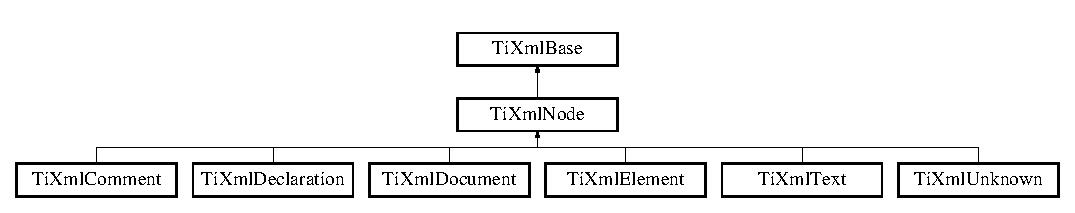
\includegraphics[height=2.413793cm]{classTiXmlNode}
\end{center}
\end{figure}
\subsection*{Public Types}
\begin{DoxyCompactItemize}
\item 
enum \textbf{ Node\+Type} \{ \newline
{\bfseries D\+O\+C\+U\+M\+E\+NT}, 
{\bfseries E\+L\+E\+M\+E\+NT}, 
{\bfseries C\+O\+M\+M\+E\+NT}, 
{\bfseries U\+N\+K\+N\+O\+WN}, 
\newline
{\bfseries T\+E\+XT}, 
{\bfseries D\+E\+C\+L\+A\+R\+A\+T\+I\+ON}, 
{\bfseries T\+Y\+P\+E\+C\+O\+U\+NT}
 \}\begin{DoxyCompactList}\small\item\em The types of X\+ML nodes supported by Tiny\+Xml. \end{DoxyCompactList}
\end{DoxyCompactItemize}
\subsection*{Public Member Functions}
\begin{DoxyCompactItemize}
\item 
const char $\ast$ \textbf{ Value} () const
\begin{DoxyCompactList}\small\item\em The meaning of \textquotesingle{}value\textquotesingle{} changes for the specific type of \doxyref{Ti\+Xml\+Node}{p.}{classTiXmlNode}. \end{DoxyCompactList}\item 
const std\+::string \& \textbf{ Value\+Str} () const
\begin{DoxyCompactList}\small\item\em Return \doxyref{Value()}{p.}{classTiXmlNode_ad44dfe927d49a74dd78b72b7514417ad} as a std\+::string. \end{DoxyCompactList}\item 
void \textbf{ Set\+Value} (const char $\ast$\+\_\+value)
\begin{DoxyCompactList}\small\item\em Changes the value of the node. \end{DoxyCompactList}\item 
\mbox{\label{classTiXmlNode_a2598d5f448042c1abbeae4503dd45ff2}} 
void \textbf{ Set\+Value} (const std\+::string \&\+\_\+value)
\begin{DoxyCompactList}\small\item\em S\+TL std\+::string form. \end{DoxyCompactList}\item 
\mbox{\label{classTiXmlNode_a708e7f953df61d4d2d12f73171550a4b}} 
void \textbf{ Clear} ()
\begin{DoxyCompactList}\small\item\em Delete all the children of this node. Does not affect \textquotesingle{}this\textquotesingle{}. \end{DoxyCompactList}\item 
\mbox{\label{classTiXmlNode_ab643043132ffd794f8602685d34a982e}} 
\textbf{ Ti\+Xml\+Node} $\ast$ \textbf{ Parent} ()
\begin{DoxyCompactList}\small\item\em One step up the D\+OM. \end{DoxyCompactList}\item 
\mbox{\label{classTiXmlNode_af13df38878a5798142693d01d6133ba0}} 
const \textbf{ Ti\+Xml\+Node} $\ast$ {\bfseries Parent} () const
\item 
\mbox{\label{classTiXmlNode_aa66bceae19707c90c1db12d7c98894a4}} 
const \textbf{ Ti\+Xml\+Node} $\ast$ \textbf{ First\+Child} () const
\begin{DoxyCompactList}\small\item\em The first child of this node. Will be null if there are no children. \end{DoxyCompactList}\item 
\mbox{\label{classTiXmlNode_a5e97d69b7c0ebd27fb7286be56559b77}} 
\textbf{ Ti\+Xml\+Node} $\ast$ {\bfseries First\+Child} ()
\item 
const \textbf{ Ti\+Xml\+Node} $\ast$ \textbf{ First\+Child} (const char $\ast$value) const
\begin{DoxyCompactList}\small\item\em The first child of this node with the matching \textquotesingle{}value\textquotesingle{}. \end{DoxyCompactList}\item 
\mbox{\label{classTiXmlNode_abc8bf32be6419ec453a731868de19554}} 
\textbf{ Ti\+Xml\+Node} $\ast$ \textbf{ First\+Child} (const char $\ast$\+\_\+value)
\begin{DoxyCompactList}\small\item\em The first child of this node with the matching \textquotesingle{}value\textquotesingle{}. Will be null if none found. \end{DoxyCompactList}\item 
\mbox{\label{classTiXmlNode_af3a04120b1ed2fead2f4bb72cbea845e}} 
const \textbf{ Ti\+Xml\+Node} $\ast$ {\bfseries Last\+Child} () const
\item 
\mbox{\label{classTiXmlNode_a6432d2b2495f6caf9cb4278df706a031}} 
\textbf{ Ti\+Xml\+Node} $\ast$ \textbf{ Last\+Child} ()
\begin{DoxyCompactList}\small\item\em The last child of this node. Will be null if there are no children. \end{DoxyCompactList}\item 
\mbox{\label{classTiXmlNode_afdd7b6ba456fdd570610c1d841f91eb3}} 
const \textbf{ Ti\+Xml\+Node} $\ast$ {\bfseries Last\+Child} (const char $\ast$value) const
\item 
\mbox{\label{classTiXmlNode_abad5bf1059c48127b958711ef89e8e5d}} 
\textbf{ Ti\+Xml\+Node} $\ast$ \textbf{ Last\+Child} (const char $\ast$\+\_\+value)
\begin{DoxyCompactList}\small\item\em The last child of this node matching \textquotesingle{}value\textquotesingle{}. Will be null if there are no children. \end{DoxyCompactList}\item 
\mbox{\label{classTiXmlNode_ab7f52e96c41fca07e81521b5f5ea35b9}} 
const \textbf{ Ti\+Xml\+Node} $\ast$ \textbf{ First\+Child} (const std\+::string \&\+\_\+value) const
\begin{DoxyCompactList}\small\item\em S\+TL std\+::string form. \end{DoxyCompactList}\item 
\mbox{\label{classTiXmlNode_a10d2669ccb5e29e02fcb0e4408685ef6}} 
\textbf{ Ti\+Xml\+Node} $\ast$ \textbf{ First\+Child} (const std\+::string \&\+\_\+value)
\begin{DoxyCompactList}\small\item\em S\+TL std\+::string form. \end{DoxyCompactList}\item 
\mbox{\label{classTiXmlNode_a96b721f14d5393dac70a0eff0d08520e}} 
const \textbf{ Ti\+Xml\+Node} $\ast$ \textbf{ Last\+Child} (const std\+::string \&\+\_\+value) const
\begin{DoxyCompactList}\small\item\em S\+TL std\+::string form. \end{DoxyCompactList}\item 
\mbox{\label{classTiXmlNode_a69772c9202f70553f940b15c06b07be3}} 
\textbf{ Ti\+Xml\+Node} $\ast$ \textbf{ Last\+Child} (const std\+::string \&\+\_\+value)
\begin{DoxyCompactList}\small\item\em S\+TL std\+::string form. \end{DoxyCompactList}\item 
const \textbf{ Ti\+Xml\+Node} $\ast$ \textbf{ Iterate\+Children} (const \textbf{ Ti\+Xml\+Node} $\ast$previous) const
\begin{DoxyCompactList}\small\item\em An alternate way to walk the children of a node. \end{DoxyCompactList}\item 
\mbox{\label{classTiXmlNode_a2358e747118fdbf0e467b1e4f7d03de1}} 
\textbf{ Ti\+Xml\+Node} $\ast$ {\bfseries Iterate\+Children} (const \textbf{ Ti\+Xml\+Node} $\ast$previous)
\item 
\mbox{\label{classTiXmlNode_a74bc68a536c279a42af346cb1454f143}} 
const \textbf{ Ti\+Xml\+Node} $\ast$ \textbf{ Iterate\+Children} (const char $\ast$value, const \textbf{ Ti\+Xml\+Node} $\ast$previous) const
\begin{DoxyCompactList}\small\item\em This flavor of Iterate\+Children searches for children with a particular \textquotesingle{}value\textquotesingle{}. \end{DoxyCompactList}\item 
\mbox{\label{classTiXmlNode_a67ba8275e533e6f76340236c42ea0aea}} 
\textbf{ Ti\+Xml\+Node} $\ast$ {\bfseries Iterate\+Children} (const char $\ast$\+\_\+value, const \textbf{ Ti\+Xml\+Node} $\ast$previous)
\item 
\mbox{\label{classTiXmlNode_a412c25b2b7e6709a4b291b13df0632eb}} 
const \textbf{ Ti\+Xml\+Node} $\ast$ \textbf{ Iterate\+Children} (const std\+::string \&\+\_\+value, const \textbf{ Ti\+Xml\+Node} $\ast$previous) const
\begin{DoxyCompactList}\small\item\em S\+TL std\+::string form. \end{DoxyCompactList}\item 
\mbox{\label{classTiXmlNode_a16e9ad53e2f5445b14bf325c90aa862c}} 
\textbf{ Ti\+Xml\+Node} $\ast$ \textbf{ Iterate\+Children} (const std\+::string \&\+\_\+value, const \textbf{ Ti\+Xml\+Node} $\ast$previous)
\begin{DoxyCompactList}\small\item\em S\+TL std\+::string form. \end{DoxyCompactList}\item 
\textbf{ Ti\+Xml\+Node} $\ast$ \textbf{ Insert\+End\+Child} (const \textbf{ Ti\+Xml\+Node} \&add\+This)
\begin{DoxyCompactList}\small\item\em Add a new node related to this. \end{DoxyCompactList}\item 
\textbf{ Ti\+Xml\+Node} $\ast$ \textbf{ Link\+End\+Child} (\textbf{ Ti\+Xml\+Node} $\ast$add\+This)
\begin{DoxyCompactList}\small\item\em Add a new node related to this. \end{DoxyCompactList}\item 
\textbf{ Ti\+Xml\+Node} $\ast$ \textbf{ Insert\+Before\+Child} (\textbf{ Ti\+Xml\+Node} $\ast$before\+This, const \textbf{ Ti\+Xml\+Node} \&add\+This)
\begin{DoxyCompactList}\small\item\em Add a new node related to this. \end{DoxyCompactList}\item 
\textbf{ Ti\+Xml\+Node} $\ast$ \textbf{ Insert\+After\+Child} (\textbf{ Ti\+Xml\+Node} $\ast$after\+This, const \textbf{ Ti\+Xml\+Node} \&add\+This)
\begin{DoxyCompactList}\small\item\em Add a new node related to this. \end{DoxyCompactList}\item 
\textbf{ Ti\+Xml\+Node} $\ast$ \textbf{ Replace\+Child} (\textbf{ Ti\+Xml\+Node} $\ast$replace\+This, const \textbf{ Ti\+Xml\+Node} \&with\+This)
\begin{DoxyCompactList}\small\item\em Replace a child of this node. \end{DoxyCompactList}\item 
\mbox{\label{classTiXmlNode_ae19d8510efc90596552f4feeac9a8fbf}} 
bool \textbf{ Remove\+Child} (\textbf{ Ti\+Xml\+Node} $\ast$remove\+This)
\begin{DoxyCompactList}\small\item\em Delete a child of this node. \end{DoxyCompactList}\item 
\mbox{\label{classTiXmlNode_a8aacf06b1a577ff0d7cfa502cc76da32}} 
const \textbf{ Ti\+Xml\+Node} $\ast$ \textbf{ Previous\+Sibling} () const
\begin{DoxyCompactList}\small\item\em Navigate to a sibling node. \end{DoxyCompactList}\item 
\mbox{\label{classTiXmlNode_af8c0642ad6ecc03f62953e68896ed1cc}} 
\textbf{ Ti\+Xml\+Node} $\ast$ {\bfseries Previous\+Sibling} ()
\item 
\mbox{\label{classTiXmlNode_ace1b618fe58b2b9305fe89bfbc8dd17b}} 
const \textbf{ Ti\+Xml\+Node} $\ast$ \textbf{ Previous\+Sibling} (const char $\ast$) const
\begin{DoxyCompactList}\small\item\em Navigate to a sibling node. \end{DoxyCompactList}\item 
\mbox{\label{classTiXmlNode_a6c977049207177ef21b51972315c2053}} 
\textbf{ Ti\+Xml\+Node} $\ast$ {\bfseries Previous\+Sibling} (const char $\ast$\+\_\+prev)
\item 
\mbox{\label{classTiXmlNode_a64ee1c722b607040cd02bd0fd05eb04a}} 
const \textbf{ Ti\+Xml\+Node} $\ast$ \textbf{ Previous\+Sibling} (const std\+::string \&\+\_\+value) const
\begin{DoxyCompactList}\small\item\em S\+TL std\+::string form. \end{DoxyCompactList}\item 
\mbox{\label{classTiXmlNode_acc8a0434c7f401d4a3b6dee77c1a5912}} 
\textbf{ Ti\+Xml\+Node} $\ast$ \textbf{ Previous\+Sibling} (const std\+::string \&\+\_\+value)
\begin{DoxyCompactList}\small\item\em S\+TL std\+::string form. \end{DoxyCompactList}\item 
\mbox{\label{classTiXmlNode_a5f0bf3809d4a35456d28cc9522c26245}} 
const \textbf{ Ti\+Xml\+Node} $\ast$ \textbf{ Next\+Sibling} (const std\+::string \&\+\_\+value) const
\begin{DoxyCompactList}\small\item\em S\+TL std\+::string form. \end{DoxyCompactList}\item 
\mbox{\label{classTiXmlNode_a1757c1f4d01e8c9596ffdbd561c76aea}} 
\textbf{ Ti\+Xml\+Node} $\ast$ \textbf{ Next\+Sibling} (const std\+::string \&\+\_\+value)
\begin{DoxyCompactList}\small\item\em S\+TL std\+::string form. \end{DoxyCompactList}\item 
\mbox{\label{classTiXmlNode_ae99c572ac7901a15993ea7a4efaa10e7}} 
const \textbf{ Ti\+Xml\+Node} $\ast$ \textbf{ Next\+Sibling} () const
\begin{DoxyCompactList}\small\item\em Navigate to a sibling node. \end{DoxyCompactList}\item 
\mbox{\label{classTiXmlNode_a4d05f7b1d7b470ac6887edd072d4892a}} 
\textbf{ Ti\+Xml\+Node} $\ast$ {\bfseries Next\+Sibling} ()
\item 
\mbox{\label{classTiXmlNode_a0864ea784b53cdca0a37829d3391ca4b}} 
const \textbf{ Ti\+Xml\+Node} $\ast$ \textbf{ Next\+Sibling} (const char $\ast$) const
\begin{DoxyCompactList}\small\item\em Navigate to a sibling node with the given \textquotesingle{}value\textquotesingle{}. \end{DoxyCompactList}\item 
\mbox{\label{classTiXmlNode_a4080bc5cc8a5c139e7cf308669e850fc}} 
\textbf{ Ti\+Xml\+Node} $\ast$ {\bfseries Next\+Sibling} (const char $\ast$\+\_\+next)
\item 
const \textbf{ Ti\+Xml\+Element} $\ast$ \textbf{ Next\+Sibling\+Element} () const
\begin{DoxyCompactList}\small\item\em Convenience function to get through elements. \end{DoxyCompactList}\item 
\mbox{\label{classTiXmlNode_a1b211cb5034655a04358e0e2f6fc5010}} 
\textbf{ Ti\+Xml\+Element} $\ast$ {\bfseries Next\+Sibling\+Element} ()
\item 
const \textbf{ Ti\+Xml\+Element} $\ast$ \textbf{ Next\+Sibling\+Element} (const char $\ast$) const
\begin{DoxyCompactList}\small\item\em Convenience function to get through elements. \end{DoxyCompactList}\item 
\mbox{\label{classTiXmlNode_a6e1ac6b800e18049bc75e9f8e63a8e5f}} 
\textbf{ Ti\+Xml\+Element} $\ast$ {\bfseries Next\+Sibling\+Element} (const char $\ast$\+\_\+next)
\item 
\mbox{\label{classTiXmlNode_a2dd7a81689a717fe5d15b3520879ff00}} 
const \textbf{ Ti\+Xml\+Element} $\ast$ \textbf{ Next\+Sibling\+Element} (const std\+::string \&\+\_\+value) const
\begin{DoxyCompactList}\small\item\em S\+TL std\+::string form. \end{DoxyCompactList}\item 
\mbox{\label{classTiXmlNode_a506958e34406729a4e4c5326ea39d081}} 
\textbf{ Ti\+Xml\+Element} $\ast$ \textbf{ Next\+Sibling\+Element} (const std\+::string \&\+\_\+value)
\begin{DoxyCompactList}\small\item\em S\+TL std\+::string form. \end{DoxyCompactList}\item 
\mbox{\label{classTiXmlNode_a12c973e1da9e90a178924b8ea5a5f4d1}} 
const \textbf{ Ti\+Xml\+Element} $\ast$ \textbf{ First\+Child\+Element} () const
\begin{DoxyCompactList}\small\item\em Convenience function to get through elements. \end{DoxyCompactList}\item 
\mbox{\label{classTiXmlNode_aa0fecff1f3866ab33a8a25506e95db1d}} 
\textbf{ Ti\+Xml\+Element} $\ast$ {\bfseries First\+Child\+Element} ()
\item 
\mbox{\label{classTiXmlNode_aab23fca4c2455c1d926c35d85a663842}} 
const \textbf{ Ti\+Xml\+Element} $\ast$ \textbf{ First\+Child\+Element} (const char $\ast$\+\_\+value) const
\begin{DoxyCompactList}\small\item\em Convenience function to get through elements. \end{DoxyCompactList}\item 
\mbox{\label{classTiXmlNode_a6936ae323675071808ac4840379e57f5}} 
\textbf{ Ti\+Xml\+Element} $\ast$ {\bfseries First\+Child\+Element} (const char $\ast$\+\_\+value)
\item 
\mbox{\label{classTiXmlNode_abfe4a2abe61324def87fe421946f9df9}} 
const \textbf{ Ti\+Xml\+Element} $\ast$ \textbf{ First\+Child\+Element} (const std\+::string \&\+\_\+value) const
\begin{DoxyCompactList}\small\item\em S\+TL std\+::string form. \end{DoxyCompactList}\item 
\mbox{\label{classTiXmlNode_a7f1d7291880534c1e5cdeb392d8c1f45}} 
\textbf{ Ti\+Xml\+Element} $\ast$ \textbf{ First\+Child\+Element} (const std\+::string \&\+\_\+value)
\begin{DoxyCompactList}\small\item\em S\+TL std\+::string form. \end{DoxyCompactList}\item 
int \textbf{ Type} () const
\begin{DoxyCompactList}\small\item\em Query the type (as an enumerated value, above) of this node. \end{DoxyCompactList}\item 
const \textbf{ Ti\+Xml\+Document} $\ast$ \textbf{ Get\+Document} () const
\begin{DoxyCompactList}\small\item\em Return a pointer to the Document this node lives in. \end{DoxyCompactList}\item 
\mbox{\label{classTiXmlNode_a7b2372c0e7adfb32f5b6902fe49a39b2}} 
\textbf{ Ti\+Xml\+Document} $\ast$ {\bfseries Get\+Document} ()
\item 
\mbox{\label{classTiXmlNode_abe85e0ec04ea59c033f324c8504653e5}} 
bool \textbf{ No\+Children} () const
\begin{DoxyCompactList}\small\item\em Returns true if this node has no children. \end{DoxyCompactList}\item 
\mbox{\label{classTiXmlNode_a775a904618cad6e4a8049bda4f5a6aa9}} 
virtual const \textbf{ Ti\+Xml\+Document} $\ast$ \textbf{ To\+Document} () const
\begin{DoxyCompactList}\small\item\em Cast to a more defined type. Will return null if not of the requested type. \end{DoxyCompactList}\item 
\mbox{\label{classTiXmlNode_a4080428f2cac46e92ef4d284202fad0b}} 
virtual const \textbf{ Ti\+Xml\+Element} $\ast$ \textbf{ To\+Element} () const
\begin{DoxyCompactList}\small\item\em Cast to a more defined type. Will return null if not of the requested type. \end{DoxyCompactList}\item 
\mbox{\label{classTiXmlNode_a5ad43b9d545315e9bb4f50d4cb70de9e}} 
virtual const \textbf{ Ti\+Xml\+Comment} $\ast$ \textbf{ To\+Comment} () const
\begin{DoxyCompactList}\small\item\em Cast to a more defined type. Will return null if not of the requested type. \end{DoxyCompactList}\item 
\mbox{\label{classTiXmlNode_ab4f2e6ce87d36c1b9b7de2529128a460}} 
virtual const \textbf{ Ti\+Xml\+Unknown} $\ast$ \textbf{ To\+Unknown} () const
\begin{DoxyCompactList}\small\item\em Cast to a more defined type. Will return null if not of the requested type. \end{DoxyCompactList}\item 
\mbox{\label{classTiXmlNode_a2591700660b308571c09166559a39332}} 
virtual const \textbf{ Ti\+Xml\+Text} $\ast$ \textbf{ To\+Text} () const
\begin{DoxyCompactList}\small\item\em Cast to a more defined type. Will return null if not of the requested type. \end{DoxyCompactList}\item 
\mbox{\label{classTiXmlNode_a0dc0831e89d499ca911a3be61a413d45}} 
virtual const \textbf{ Ti\+Xml\+Declaration} $\ast$ \textbf{ To\+Declaration} () const
\begin{DoxyCompactList}\small\item\em Cast to a more defined type. Will return null if not of the requested type. \end{DoxyCompactList}\item 
\mbox{\label{classTiXmlNode_a6a4c8ac28ee7a745d059db6691e03bae}} 
virtual \textbf{ Ti\+Xml\+Document} $\ast$ \textbf{ To\+Document} ()
\begin{DoxyCompactList}\small\item\em Cast to a more defined type. Will return null if not of the requested type. \end{DoxyCompactList}\item 
\mbox{\label{classTiXmlNode_aa65d000223187d22a4dcebd7479e9ebc}} 
virtual \textbf{ Ti\+Xml\+Element} $\ast$ \textbf{ To\+Element} ()
\begin{DoxyCompactList}\small\item\em Cast to a more defined type. Will return null if not of the requested type. \end{DoxyCompactList}\item 
\mbox{\label{classTiXmlNode_a383e06a0787f7063953934867990f849}} 
virtual \textbf{ Ti\+Xml\+Comment} $\ast$ \textbf{ To\+Comment} ()
\begin{DoxyCompactList}\small\item\em Cast to a more defined type. Will return null if not of the requested type. \end{DoxyCompactList}\item 
\mbox{\label{classTiXmlNode_a06de5af852668c7e4af0d09c205f0b0d}} 
virtual \textbf{ Ti\+Xml\+Unknown} $\ast$ \textbf{ To\+Unknown} ()
\begin{DoxyCompactList}\small\item\em Cast to a more defined type. Will return null if not of the requested type. \end{DoxyCompactList}\item 
\mbox{\label{classTiXmlNode_a3ddfbcac78fbea041fad57e5c6d60a03}} 
virtual \textbf{ Ti\+Xml\+Text} $\ast$ \textbf{ To\+Text} ()
\begin{DoxyCompactList}\small\item\em Cast to a more defined type. Will return null if not of the requested type. \end{DoxyCompactList}\item 
\mbox{\label{classTiXmlNode_a4027136ca820ff4a636b607231b6a6df}} 
virtual \textbf{ Ti\+Xml\+Declaration} $\ast$ \textbf{ To\+Declaration} ()
\begin{DoxyCompactList}\small\item\em Cast to a more defined type. Will return null if not of the requested type. \end{DoxyCompactList}\item 
virtual \textbf{ Ti\+Xml\+Node} $\ast$ \textbf{ Clone} () const =0
\begin{DoxyCompactList}\small\item\em Create an exact duplicate of this node and return it. \end{DoxyCompactList}\item 
virtual bool \textbf{ Accept} (\textbf{ Ti\+Xml\+Visitor} $\ast$visitor) const =0
\begin{DoxyCompactList}\small\item\em Accept a hierchical visit the nodes in the Tiny\+X\+ML D\+OM. \end{DoxyCompactList}\end{DoxyCompactItemize}
\subsection*{Protected Member Functions}
\begin{DoxyCompactItemize}
\item 
\mbox{\label{classTiXmlNode_a3f46721695868667113c7487ff123f20}} 
{\bfseries Ti\+Xml\+Node} (\textbf{ Node\+Type} \+\_\+type)
\item 
\mbox{\label{classTiXmlNode_aaadd5bb9c94f84c4472b649b95de4a0b}} 
void {\bfseries Copy\+To} (\textbf{ Ti\+Xml\+Node} $\ast$target) const
\item 
\mbox{\label{classTiXmlNode_ab4b4af1a6b486dcbc0e327cf291270af}} 
virtual void {\bfseries Stream\+In} (std\+::istream $\ast$in, T\+I\+X\+M\+L\+\_\+\+S\+T\+R\+I\+NG $\ast$tag)=0
\item 
\mbox{\label{classTiXmlNode_ac1e3a8e7578be463b04617786120c2bb}} 
\textbf{ Ti\+Xml\+Node} $\ast$ {\bfseries Identify} (const char $\ast$start, Ti\+Xml\+Encoding encoding)
\end{DoxyCompactItemize}
\subsection*{Protected Attributes}
\begin{DoxyCompactItemize}
\item 
\mbox{\label{classTiXmlNode_a662c4de61244e4fa5bd4e2d8c63143a5}} 
\textbf{ Ti\+Xml\+Node} $\ast$ {\bfseries parent}
\item 
\mbox{\label{classTiXmlNode_a2619c6379181c16ba95ae6922e2ca839}} 
\textbf{ Node\+Type} {\bfseries type}
\item 
\mbox{\label{classTiXmlNode_af749fb7f22010b80e8f904c32653d50e}} 
\textbf{ Ti\+Xml\+Node} $\ast$ {\bfseries first\+Child}
\item 
\mbox{\label{classTiXmlNode_a5b30756d21b304580d22a841ec9d61f8}} 
\textbf{ Ti\+Xml\+Node} $\ast$ {\bfseries last\+Child}
\item 
\mbox{\label{classTiXmlNode_aead528b3cedc33c16a6c539872c7cc8b}} 
T\+I\+X\+M\+L\+\_\+\+S\+T\+R\+I\+NG {\bfseries value}
\item 
\mbox{\label{classTiXmlNode_a9c5370ea2cbfd9f0e0f7b30a57fd68f5}} 
\textbf{ Ti\+Xml\+Node} $\ast$ {\bfseries prev}
\item 
\mbox{\label{classTiXmlNode_a2f329cc993d2d34df76e17dcbb776b45}} 
\textbf{ Ti\+Xml\+Node} $\ast$ {\bfseries next}
\end{DoxyCompactItemize}
\subsection*{Friends}
\begin{DoxyCompactItemize}
\item 
\mbox{\label{classTiXmlNode_a173617f6dfe902cf484ce5552b950475}} 
class {\bfseries Ti\+Xml\+Document}
\item 
\mbox{\label{classTiXmlNode_ab6592e32cb9132be517cc12a70564c4b}} 
class {\bfseries Ti\+Xml\+Element}
\item 
std\+::istream \& \textbf{ operator$>$$>$} (std\+::istream \&in, \textbf{ Ti\+Xml\+Node} \&base)
\begin{DoxyCompactList}\small\item\em An input stream operator, for every class. \end{DoxyCompactList}\item 
std\+::ostream \& \textbf{ operator$<$$<$} (std\+::ostream \&out, const \textbf{ Ti\+Xml\+Node} \&base)
\begin{DoxyCompactList}\small\item\em An output stream operator, for every class. \end{DoxyCompactList}\item 
\mbox{\label{classTiXmlNode_a52ef17e7080df2490cf87bde380685ab}} 
std\+::string \& \textbf{ operator$<$$<$} (std\+::string \&out, const \textbf{ Ti\+Xml\+Node} \&base)
\begin{DoxyCompactList}\small\item\em Appends the X\+ML node or attribute to a std\+::string. \end{DoxyCompactList}\end{DoxyCompactItemize}
\subsection*{Additional Inherited Members}


\subsection{Detailed Description}
The parent class for everything in the Document Object Model. 

(Except for attributes). Nodes have siblings, a parent, and children. A node can be in a document, or stand on its own. The type of a \doxyref{Ti\+Xml\+Node}{p.}{classTiXmlNode} can be queried, and it can be cast to its more defined type. 

\subsection{Member Enumeration Documentation}
\mbox{\label{classTiXmlNode_a836eded4920ab9e9ef28496f48cd95a2}} 
\index{Ti\+Xml\+Node@{Ti\+Xml\+Node}!Node\+Type@{Node\+Type}}
\index{Node\+Type@{Node\+Type}!Ti\+Xml\+Node@{Ti\+Xml\+Node}}
\subsubsection{Node\+Type}
{\footnotesize\ttfamily enum \textbf{ Ti\+Xml\+Node\+::\+Node\+Type}}



The types of X\+ML nodes supported by Tiny\+Xml. 

(All the unsupported types are picked up by U\+N\+K\+N\+O\+WN.) 

\subsection{Member Function Documentation}
\mbox{\label{classTiXmlNode_acc0f88b7462c6cb73809d410a4f5bb86}} 
\index{Ti\+Xml\+Node@{Ti\+Xml\+Node}!Accept@{Accept}}
\index{Accept@{Accept}!Ti\+Xml\+Node@{Ti\+Xml\+Node}}
\subsubsection{Accept()}
{\footnotesize\ttfamily virtual bool Ti\+Xml\+Node\+::\+Accept (\begin{DoxyParamCaption}\item[{\textbf{ Ti\+Xml\+Visitor} $\ast$}]{visitor }\end{DoxyParamCaption}) const\hspace{0.3cm}{\ttfamily [pure virtual]}}



Accept a hierchical visit the nodes in the Tiny\+X\+ML D\+OM. 

Every node in the X\+ML tree will be conditionally visited and the host will be called back via the \doxyref{Ti\+Xml\+Visitor}{p.}{classTiXmlVisitor} interface.

This is essentially a S\+AX interface for Tiny\+X\+ML. (Note however it doesn\textquotesingle{}t re-\/parse the X\+ML for the callbacks, so the performance of Tiny\+X\+ML is unchanged by using this interface versus any other.)

The interface has been based on ideas from\+:


\begin{DoxyItemize}
\item {\tt http\+://www.\+saxproject.\+org/}
\item {\tt http\+://c2.\+com/cgi/wiki?\+Hierarchical\+Visitor\+Pattern}
\end{DoxyItemize}

Which are both good references for \char`\"{}visiting\char`\"{}.

An example of using \doxyref{Accept()}{p.}{classTiXmlNode_acc0f88b7462c6cb73809d410a4f5bb86}\+: \begin{DoxyVerb}    TiXmlPrinter printer;
    tinyxmlDoc.Accept( &printer );
    const char* xmlcstr = printer.CStr();\end{DoxyVerb}
 

Implemented in \textbf{ Ti\+Xml\+Document} \doxyref{}{p.}{classTiXmlDocument_a8ddd6eec722cbd25900bbac664909bac}, \textbf{ Ti\+Xml\+Unknown} \doxyref{}{p.}{classTiXmlUnknown_aafdf1b2d4f561979c7907bad91004999}, \textbf{ Ti\+Xml\+Declaration} \doxyref{}{p.}{classTiXmlDeclaration_aa1b6bade6c989407ce9881bdfc73c1e6}, \textbf{ Ti\+Xml\+Text} \doxyref{}{p.}{classTiXmlText_af65964326eac4640bfb97d4622fa0de2}, \textbf{ Ti\+Xml\+Comment} \doxyref{}{p.}{classTiXmlComment_ac894241530d1d266131a5026cb251a95}, and \textbf{ Ti\+Xml\+Element} \doxyref{}{p.}{classTiXmlElement_a01d33358cce9d1817b557d314dda3779}.



Referenced by Ti\+Xml\+Element\+::\+Accept(), Ti\+Xml\+Document\+::\+Accept(), and Ti\+Xml\+Unknown\+::\+Clone().

\mbox{\label{classTiXmlNode_a4508cc3a2d7a98e96a54cc09c37a78a4}} 
\index{Ti\+Xml\+Node@{Ti\+Xml\+Node}!Clone@{Clone}}
\index{Clone@{Clone}!Ti\+Xml\+Node@{Ti\+Xml\+Node}}
\subsubsection{Clone()}
{\footnotesize\ttfamily virtual \textbf{ Ti\+Xml\+Node}$\ast$ Ti\+Xml\+Node\+::\+Clone (\begin{DoxyParamCaption}{ }\end{DoxyParamCaption}) const\hspace{0.3cm}{\ttfamily [pure virtual]}}



Create an exact duplicate of this node and return it. 

The memory must be deleted by the caller. 

Implemented in \textbf{ Ti\+Xml\+Document} \doxyref{}{p.}{classTiXmlDocument_a46a4dda6c56eb106d46d4046ae1e5353}, \textbf{ Ti\+Xml\+Unknown} \doxyref{}{p.}{classTiXmlUnknown_a3dea7689de5b1931fd6657992948fde0}, \textbf{ Ti\+Xml\+Declaration} \doxyref{}{p.}{classTiXmlDeclaration_a35dc1455f69b79e81cae28e186944610}, \textbf{ Ti\+Xml\+Text} \doxyref{}{p.}{classTiXmlText_a98a20d7a4f1c1478e25e34921be24bfe}, \textbf{ Ti\+Xml\+Comment} \doxyref{}{p.}{classTiXmlComment_a1f9f06e2ed3f77875093436193b16c16}, and \textbf{ Ti\+Xml\+Element} \doxyref{}{p.}{classTiXmlElement_a810ea8fa40844c01334e5af2a26794cb}.



Referenced by Insert\+After\+Child(), Insert\+Before\+Child(), Insert\+End\+Child(), marlin\+::\+X\+M\+L\+Parser\+::parse(), Ti\+Xml\+Element\+::\+Print(), marlin\+::\+X\+M\+L\+Parser\+::processconditions(), Replace\+Child(), and Ti\+Xml\+Document\+::\+Save\+File().

\mbox{\label{classTiXmlNode_ae98c367f664890c4b5a5183481ec128a}} 
\index{Ti\+Xml\+Node@{Ti\+Xml\+Node}!First\+Child@{First\+Child}}
\index{First\+Child@{First\+Child}!Ti\+Xml\+Node@{Ti\+Xml\+Node}}
\subsubsection{First\+Child()}
{\footnotesize\ttfamily const \textbf{ Ti\+Xml\+Node} $\ast$ Ti\+Xml\+Node\+::\+First\+Child (\begin{DoxyParamCaption}\item[{const char $\ast$}]{value }\end{DoxyParamCaption}) const}



The first child of this node with the matching \textquotesingle{}value\textquotesingle{}. 

Will be null if none found. 

References Value().

\mbox{\label{classTiXmlNode_adcb070acefcbaedaa0673d82e530538b}} 
\index{Ti\+Xml\+Node@{Ti\+Xml\+Node}!Get\+Document@{Get\+Document}}
\index{Get\+Document@{Get\+Document}!Ti\+Xml\+Node@{Ti\+Xml\+Node}}
\subsubsection{Get\+Document()}
{\footnotesize\ttfamily const \textbf{ Ti\+Xml\+Document} $\ast$ Ti\+Xml\+Node\+::\+Get\+Document (\begin{DoxyParamCaption}{ }\end{DoxyParamCaption}) const}



Return a pointer to the Document this node lives in. 

Returns null if not in a document. 

References To\+Document().



Referenced by Link\+End\+Child(), Ti\+Xml\+Document\+::\+Parse(), marlin\+::\+X\+M\+L\+Parser\+::process\+Include\+Elements(), Ti\+Xml\+Element\+::\+Set\+Attribute(), and Type().

\mbox{\label{classTiXmlNode_a274db3292218202805c093f66a964cb5}} 
\index{Ti\+Xml\+Node@{Ti\+Xml\+Node}!Insert\+After\+Child@{Insert\+After\+Child}}
\index{Insert\+After\+Child@{Insert\+After\+Child}!Ti\+Xml\+Node@{Ti\+Xml\+Node}}
\subsubsection{Insert\+After\+Child()}
{\footnotesize\ttfamily \textbf{ Ti\+Xml\+Node} $\ast$ Ti\+Xml\+Node\+::\+Insert\+After\+Child (\begin{DoxyParamCaption}\item[{\textbf{ Ti\+Xml\+Node} $\ast$}]{after\+This,  }\item[{const \textbf{ Ti\+Xml\+Node} \&}]{add\+This }\end{DoxyParamCaption})}



Add a new node related to this. 

Adds a child after the specified child. Returns a pointer to the new object or N\+U\+LL if an error occured. 

References Clone(), and Type().



Referenced by Iterate\+Children(), and marlin\+::\+X\+M\+L\+Parser\+::process\+Include\+Elements().

\mbox{\label{classTiXmlNode_a71e54e393336382bc9875f64aab5cb15}} 
\index{Ti\+Xml\+Node@{Ti\+Xml\+Node}!Insert\+Before\+Child@{Insert\+Before\+Child}}
\index{Insert\+Before\+Child@{Insert\+Before\+Child}!Ti\+Xml\+Node@{Ti\+Xml\+Node}}
\subsubsection{Insert\+Before\+Child()}
{\footnotesize\ttfamily \textbf{ Ti\+Xml\+Node} $\ast$ Ti\+Xml\+Node\+::\+Insert\+Before\+Child (\begin{DoxyParamCaption}\item[{\textbf{ Ti\+Xml\+Node} $\ast$}]{before\+This,  }\item[{const \textbf{ Ti\+Xml\+Node} \&}]{add\+This }\end{DoxyParamCaption})}



Add a new node related to this. 

Adds a child before the specified child. Returns a pointer to the new object or N\+U\+LL if an error occured. 

References Clone(), and Type().



Referenced by Iterate\+Children(), marlin\+::\+X\+M\+L\+Parser\+::parse(), marlin\+::\+X\+M\+L\+Parser\+::processconditions(), and marlin\+::\+X\+M\+L\+Parser\+::replacegroups().

\mbox{\label{classTiXmlNode_af287a913ce46d8dbf7ef24fec69bbaf0}} 
\index{Ti\+Xml\+Node@{Ti\+Xml\+Node}!Insert\+End\+Child@{Insert\+End\+Child}}
\index{Insert\+End\+Child@{Insert\+End\+Child}!Ti\+Xml\+Node@{Ti\+Xml\+Node}}
\subsubsection{Insert\+End\+Child()}
{\footnotesize\ttfamily \textbf{ Ti\+Xml\+Node} $\ast$ Ti\+Xml\+Node\+::\+Insert\+End\+Child (\begin{DoxyParamCaption}\item[{const \textbf{ Ti\+Xml\+Node} \&}]{add\+This }\end{DoxyParamCaption})}



Add a new node related to this. 

Adds a child past the Last\+Child. Returns a pointer to the new object or N\+U\+LL if an error occured. 

References Clone(), and Type().



Referenced by Iterate\+Children(), and marlin\+::\+X\+M\+L\+Parser\+::parse().

\mbox{\label{classTiXmlNode_a67c3a02b797f08d9a31b2553661257e1}} 
\index{Ti\+Xml\+Node@{Ti\+Xml\+Node}!Iterate\+Children@{Iterate\+Children}}
\index{Iterate\+Children@{Iterate\+Children}!Ti\+Xml\+Node@{Ti\+Xml\+Node}}
\subsubsection{Iterate\+Children()}
{\footnotesize\ttfamily const \textbf{ Ti\+Xml\+Node} $\ast$ Ti\+Xml\+Node\+::\+Iterate\+Children (\begin{DoxyParamCaption}\item[{const \textbf{ Ti\+Xml\+Node} $\ast$}]{previous }\end{DoxyParamCaption}) const}



An alternate way to walk the children of a node. 

One way to iterate over nodes is\+: \begin{DoxyVerb}        for( child = parent->FirstChild(); child; child = child->NextSibling() )\end{DoxyVerb}


Iterate\+Children does the same thing with the syntax\+: \begin{DoxyVerb}        child = 0;
        while( child = parent->IterateChildren( child ) )\end{DoxyVerb}


Iterate\+Children takes the previous child as input and finds the next one. If the previous child is null, it returns the first. Iterate\+Children will return null when done. 

References Next\+Sibling().



Referenced by marlin\+::\+X\+M\+L\+Parser\+::find\+Element(), Last\+Child(), marlin\+::\+X\+M\+L\+Parser\+::parameters\+From\+Node(), marlin\+::\+X\+M\+L\+Parser\+::parse(), marlin\+::\+X\+M\+L\+Parser\+::processconditions(), and marlin\+::\+X\+M\+L\+Parser\+::replacegroups().

\mbox{\label{classTiXmlNode_a1a881212554b759865f6cac79a851d38}} 
\index{Ti\+Xml\+Node@{Ti\+Xml\+Node}!Link\+End\+Child@{Link\+End\+Child}}
\index{Link\+End\+Child@{Link\+End\+Child}!Ti\+Xml\+Node@{Ti\+Xml\+Node}}
\subsubsection{Link\+End\+Child()}
{\footnotesize\ttfamily \textbf{ Ti\+Xml\+Node} $\ast$ Ti\+Xml\+Node\+::\+Link\+End\+Child (\begin{DoxyParamCaption}\item[{\textbf{ Ti\+Xml\+Node} $\ast$}]{add\+This }\end{DoxyParamCaption})}



Add a new node related to this. 

Adds a child past the Last\+Child.

N\+O\+TE\+: the node to be added is passed by pointer, and will be henceforth owned (and deleted) by tiny\+Xml. This method is efficient and avoids an extra copy, but should be used with care as it uses a different memory model than the other insert functions.

\begin{DoxySeeAlso}{See also}
\doxyref{Insert\+End\+Child}{p.}{classTiXmlNode_af287a913ce46d8dbf7ef24fec69bbaf0} 
\end{DoxySeeAlso}


References Get\+Document(), and Type().



Referenced by Iterate\+Children(), Ti\+Xml\+Document\+::\+Parse(), Ti\+Xml\+Element\+::\+Print(), and Ti\+Xml\+Document\+::\+Save\+File().

\mbox{\label{classTiXmlNode_ac6105781c913a42aa7f3f17bd1964f7c}} 
\index{Ti\+Xml\+Node@{Ti\+Xml\+Node}!Next\+Sibling\+Element@{Next\+Sibling\+Element}}
\index{Next\+Sibling\+Element@{Next\+Sibling\+Element}!Ti\+Xml\+Node@{Ti\+Xml\+Node}}
\subsubsection{Next\+Sibling\+Element()\hspace{0.1cm}{\footnotesize\ttfamily [1/2]}}
{\footnotesize\ttfamily const \textbf{ Ti\+Xml\+Element} $\ast$ Ti\+Xml\+Node\+::\+Next\+Sibling\+Element (\begin{DoxyParamCaption}{ }\end{DoxyParamCaption}) const}



Convenience function to get through elements. 

Calls Next\+Sibling and To\+Element. Will skip all non-\/\+Element nodes. Returns 0 if there is not another element. 

References Next\+Sibling(), and To\+Element().



Referenced by Ti\+Xml\+Handle\+::\+Child\+Element(), Next\+Sibling(), marlin\+::\+X\+M\+L\+Parser\+::parse(), and marlin\+::\+X\+M\+L\+Parser\+::process\+Include\+Elements().

\mbox{\label{classTiXmlNode_a22def4746238abaee042f99b47ef3c94}} 
\index{Ti\+Xml\+Node@{Ti\+Xml\+Node}!Next\+Sibling\+Element@{Next\+Sibling\+Element}}
\index{Next\+Sibling\+Element@{Next\+Sibling\+Element}!Ti\+Xml\+Node@{Ti\+Xml\+Node}}
\subsubsection{Next\+Sibling\+Element()\hspace{0.1cm}{\footnotesize\ttfamily [2/2]}}
{\footnotesize\ttfamily const \textbf{ Ti\+Xml\+Element} $\ast$ Ti\+Xml\+Node\+::\+Next\+Sibling\+Element (\begin{DoxyParamCaption}\item[{const char $\ast$}]{\+\_\+value }\end{DoxyParamCaption}) const}



Convenience function to get through elements. 

Calls Next\+Sibling and To\+Element. Will skip all non-\/\+Element nodes. Returns 0 if there is not another element. 

References Next\+Sibling(), and To\+Element().

\mbox{\label{classTiXmlNode_a543208c2c801c84a213529541e904b9f}} 
\index{Ti\+Xml\+Node@{Ti\+Xml\+Node}!Replace\+Child@{Replace\+Child}}
\index{Replace\+Child@{Replace\+Child}!Ti\+Xml\+Node@{Ti\+Xml\+Node}}
\subsubsection{Replace\+Child()}
{\footnotesize\ttfamily \textbf{ Ti\+Xml\+Node} $\ast$ Ti\+Xml\+Node\+::\+Replace\+Child (\begin{DoxyParamCaption}\item[{\textbf{ Ti\+Xml\+Node} $\ast$}]{replace\+This,  }\item[{const \textbf{ Ti\+Xml\+Node} \&}]{with\+This }\end{DoxyParamCaption})}



Replace a child of this node. 

Returns a pointer to the new object or N\+U\+LL if an error occured. 

References Clone().



Referenced by Iterate\+Children().

\mbox{\label{classTiXmlNode_a2a38329ca5d3f28f98ce932b8299ae90}} 
\index{Ti\+Xml\+Node@{Ti\+Xml\+Node}!Set\+Value@{Set\+Value}}
\index{Set\+Value@{Set\+Value}!Ti\+Xml\+Node@{Ti\+Xml\+Node}}
\subsubsection{Set\+Value()}
{\footnotesize\ttfamily void Ti\+Xml\+Node\+::\+Set\+Value (\begin{DoxyParamCaption}\item[{const char $\ast$}]{\+\_\+value }\end{DoxyParamCaption})\hspace{0.3cm}{\ttfamily [inline]}}



Changes the value of the node. 

Defined as\+: \begin{DoxyVerb}    Document:   filename of the xml file
    Element:    name of the element
    Comment:    the comment text
    Unknown:    the tag contents
    Text:               the text string\end{DoxyVerb}
 

References Clear().



Referenced by marlin\+::\+X\+M\+L\+Parser\+::parameters\+From\+Node(), marlin\+::\+X\+M\+L\+Parser\+::process\+Include\+Elements(), Ti\+Xml\+Attribute\+::\+Set\+Double\+Value(), Ti\+Xml\+Attribute\+::\+Set\+Int\+Value(), and Ti\+Xml\+Text\+::\+Ti\+Xml\+Text().

\mbox{\label{classTiXmlNode_a0f4dd916b2afc2ab2f1a84f3e2b8fd5d}} 
\index{Ti\+Xml\+Node@{Ti\+Xml\+Node}!Type@{Type}}
\index{Type@{Type}!Ti\+Xml\+Node@{Ti\+Xml\+Node}}
\subsubsection{Type()}
{\footnotesize\ttfamily int Ti\+Xml\+Node\+::\+Type (\begin{DoxyParamCaption}{ }\end{DoxyParamCaption}) const\hspace{0.3cm}{\ttfamily [inline]}}



Query the type (as an enumerated value, above) of this node. 

The possible types are\+: D\+O\+C\+U\+M\+E\+NT, E\+L\+E\+M\+E\+NT, C\+O\+M\+M\+E\+NT, U\+N\+K\+N\+O\+WN, T\+E\+XT, and D\+E\+C\+L\+A\+R\+A\+T\+I\+ON. 

References Get\+Document().



Referenced by Insert\+After\+Child(), Insert\+Before\+Child(), Insert\+End\+Child(), and Link\+End\+Child().

\mbox{\label{classTiXmlNode_ad44dfe927d49a74dd78b72b7514417ad}} 
\index{Ti\+Xml\+Node@{Ti\+Xml\+Node}!Value@{Value}}
\index{Value@{Value}!Ti\+Xml\+Node@{Ti\+Xml\+Node}}
\subsubsection{Value()}
{\footnotesize\ttfamily const char$\ast$ Ti\+Xml\+Node\+::\+Value (\begin{DoxyParamCaption}{ }\end{DoxyParamCaption}) const\hspace{0.3cm}{\ttfamily [inline]}}



The meaning of \textquotesingle{}value\textquotesingle{} changes for the specific type of \doxyref{Ti\+Xml\+Node}{p.}{classTiXmlNode}. 

\begin{DoxyVerb}    Document:   filename of the xml file
    Element:    name of the element
    Comment:    the comment text
    Unknown:    the tag contents
    Text:               the text string\end{DoxyVerb}


The subclasses will wrap this function. 

Referenced by Ti\+Xml\+Element\+::\+Clone(), First\+Child(), marlin\+::\+X\+M\+L\+Parser\+::get\+Attribute(), Ti\+Xml\+Element\+::\+Get\+Text(), Ti\+Xml\+Document\+::\+Load\+File(), Next\+Sibling(), marlin\+::\+X\+M\+L\+Parser\+::parameters\+From\+Node(), Previous\+Sibling(), marlin\+::\+X\+M\+L\+Parser\+::processconditions(), marlin\+::\+X\+M\+L\+Parser\+::process\+Include\+Elements(), marlin\+::\+X\+M\+L\+Parser\+::replacegroups(), Ti\+Xml\+Document\+::\+Save\+File(), Ti\+Xml\+Printer\+::\+Visit(), Ti\+Xml\+Printer\+::\+Visit\+Enter(), and Ti\+Xml\+Printer\+::\+Visit\+Exit().

\mbox{\label{classTiXmlNode_a74bda074919e4a5e08d700204793f898}} 
\index{Ti\+Xml\+Node@{Ti\+Xml\+Node}!Value\+Str@{Value\+Str}}
\index{Value\+Str@{Value\+Str}!Ti\+Xml\+Node@{Ti\+Xml\+Node}}
\subsubsection{Value\+Str()}
{\footnotesize\ttfamily const std\+::string\& Ti\+Xml\+Node\+::\+Value\+Str (\begin{DoxyParamCaption}{ }\end{DoxyParamCaption}) const\hspace{0.3cm}{\ttfamily [inline]}}



Return \doxyref{Value()}{p.}{classTiXmlNode_ad44dfe927d49a74dd78b72b7514417ad} as a std\+::string. 

If you only use S\+TL, this is more efficient than calling \doxyref{Value()}{p.}{classTiXmlNode_ad44dfe927d49a74dd78b72b7514417ad}. Only available in S\+TL mode. 

\subsection{Friends And Related Function Documentation}
\mbox{\label{classTiXmlNode_a86cd49cfb17a844c0010b3136ac966c7}} 
\index{Ti\+Xml\+Node@{Ti\+Xml\+Node}!operator$<$$<$@{operator$<$$<$}}
\index{operator$<$$<$@{operator$<$$<$}!Ti\+Xml\+Node@{Ti\+Xml\+Node}}
\subsubsection{operator$<$$<$}
{\footnotesize\ttfamily std\+::ostream\& operator$<$$<$ (\begin{DoxyParamCaption}\item[{std\+::ostream \&}]{out,  }\item[{const \textbf{ Ti\+Xml\+Node} \&}]{base }\end{DoxyParamCaption})\hspace{0.3cm}{\ttfamily [friend]}}



An output stream operator, for every class. 

Note that this outputs without any newlines or formatting, as opposed to \doxyref{Print()}{p.}{classTiXmlBase_a0de56b3f2ef14c65091a3b916437b512}, which includes tabs and new lines.

The operator$<$$<$ and operator$>$$>$ are not completely symmetric. Writing a node to a stream is very well defined. You\textquotesingle{}ll get a nice stream of output, without any extra whitespace or newlines.

But reading is not as well defined. (As it always is.) If you create a \doxyref{Ti\+Xml\+Element}{p.}{classTiXmlElement} (for example) and read that from an input stream, the text needs to define an element or junk will result. This is true of all input streams, but it\textquotesingle{}s worth keeping in mind.

A \doxyref{Ti\+Xml\+Document}{p.}{classTiXmlDocument} will read nodes until it reads a root element, and all the children of that root element. 

Referenced by Ti\+Xml\+Unknown\+::\+Clone().

\mbox{\label{classTiXmlNode_ab57bd426563c926844f65a78412e18b9}} 
\index{Ti\+Xml\+Node@{Ti\+Xml\+Node}!operator$>$$>$@{operator$>$$>$}}
\index{operator$>$$>$@{operator$>$$>$}!Ti\+Xml\+Node@{Ti\+Xml\+Node}}
\subsubsection{operator$>$$>$}
{\footnotesize\ttfamily std\+::istream\& operator$>$$>$ (\begin{DoxyParamCaption}\item[{std\+::istream \&}]{in,  }\item[{\textbf{ Ti\+Xml\+Node} \&}]{base }\end{DoxyParamCaption})\hspace{0.3cm}{\ttfamily [friend]}}



An input stream operator, for every class. 

Tolerant of newlines and formatting, but doesn\textquotesingle{}t expect them. 

Referenced by Ti\+Xml\+Unknown\+::\+Clone().



The documentation for this class was generated from the following files\+:\begin{DoxyCompactItemize}
\item 
tinyxml.\+h\item 
tinyxml.\+cc\item 
tinyxmlparser.\+cc\end{DoxyCompactItemize}

\section{Ti\+Xml\+Out\+Stream Class Reference}
\label{classTiXmlOutStream}\index{Ti\+Xml\+Out\+Stream@{Ti\+Xml\+Out\+Stream}}
Inheritance diagram for Ti\+Xml\+Out\+Stream\+:\begin{figure}[H]
\begin{center}
\leavevmode
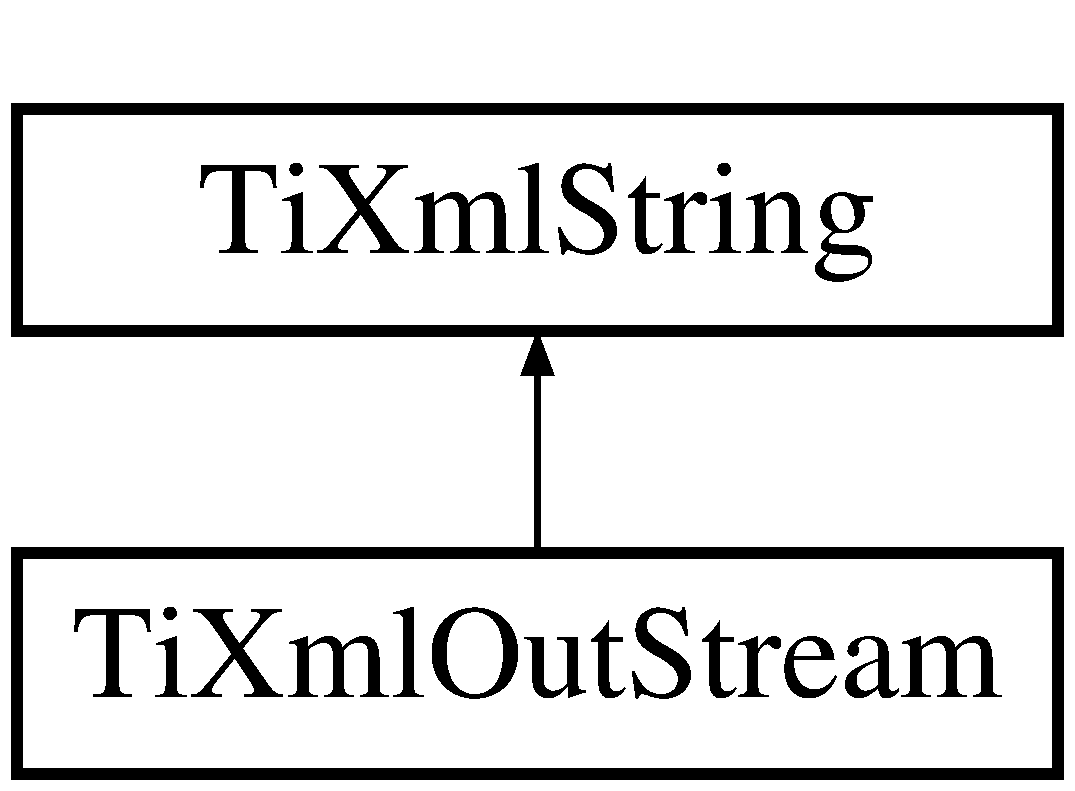
\includegraphics[height=2.000000cm]{classTiXmlOutStream}
\end{center}
\end{figure}
\subsection*{Public Member Functions}
\begin{DoxyCompactItemize}
\item 
\mbox{\label{classTiXmlOutStream_a3640dcb1c0903be3bc6966cdc9a79db6}} 
\textbf{ Ti\+Xml\+Out\+Stream} \& {\bfseries operator$<$$<$} (const \textbf{ Ti\+Xml\+String} \&in)
\item 
\mbox{\label{classTiXmlOutStream_af2117e5a8cbfcb69544804ad2859bfb6}} 
\textbf{ Ti\+Xml\+Out\+Stream} \& {\bfseries operator$<$$<$} (const char $\ast$in)
\end{DoxyCompactItemize}
\subsection*{Additional Inherited Members}


The documentation for this class was generated from the following file\+:\begin{DoxyCompactItemize}
\item 
tinystr.\+h\end{DoxyCompactItemize}

\section{Ti\+Xml\+Parsing\+Data Class Reference}
\label{classTiXmlParsingData}\index{Ti\+Xml\+Parsing\+Data@{Ti\+Xml\+Parsing\+Data}}
\subsection*{Public Member Functions}
\begin{DoxyCompactItemize}
\item 
\mbox{\label{classTiXmlParsingData_a65cee8ab77a36c605db08c84b4c30a7d}} 
void {\bfseries Stamp} (const char $\ast$now, Ti\+Xml\+Encoding encoding)
\item 
\mbox{\label{classTiXmlParsingData_a56908a17d7d7a6b2e511e62cf1d40d05}} 
const \textbf{ Ti\+Xml\+Cursor} \& {\bfseries Cursor} ()
\end{DoxyCompactItemize}
\subsection*{Friends}
\begin{DoxyCompactItemize}
\item 
\mbox{\label{classTiXmlParsingData_a173617f6dfe902cf484ce5552b950475}} 
class {\bfseries Ti\+Xml\+Document}
\end{DoxyCompactItemize}


The documentation for this class was generated from the following file\+:\begin{DoxyCompactItemize}
\item 
tinyxmlparser.\+cc\end{DoxyCompactItemize}

\section{Ti\+Xml\+Printer Class Reference}
\label{classTiXmlPrinter}\index{Ti\+Xml\+Printer@{Ti\+Xml\+Printer}}


Print to memory functionality.  




{\ttfamily \#include $<$tinyxml.\+h$>$}

Inheritance diagram for Ti\+Xml\+Printer\+:\begin{figure}[H]
\begin{center}
\leavevmode
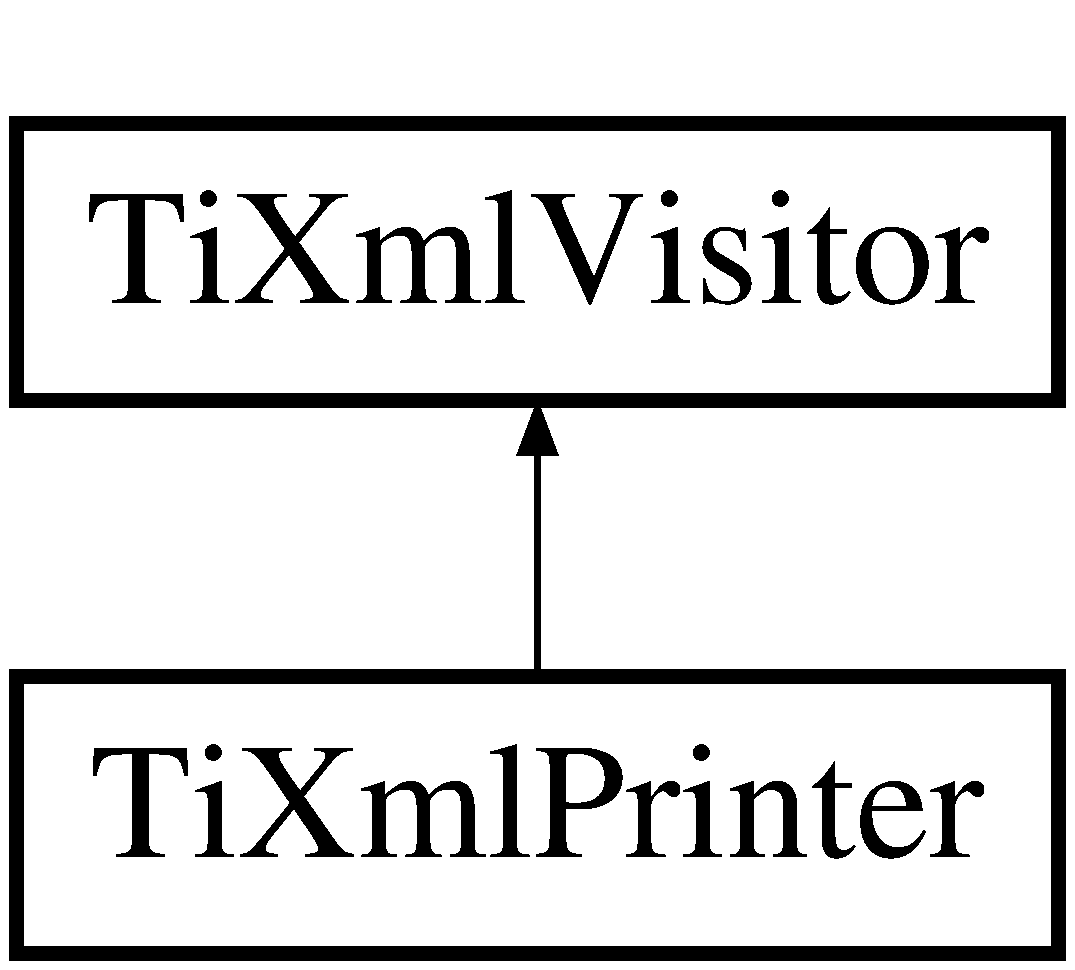
\includegraphics[height=2.000000cm]{classTiXmlPrinter}
\end{center}
\end{figure}
\subsection*{Public Member Functions}
\begin{DoxyCompactItemize}
\item 
\mbox{\label{classTiXmlPrinter_a2ec73087db26ff4d2c4316c56f861db7}} 
virtual bool \textbf{ Visit\+Enter} (const \textbf{ Ti\+Xml\+Document} \&doc)
\begin{DoxyCompactList}\small\item\em Visit a document. \end{DoxyCompactList}\item 
\mbox{\label{classTiXmlPrinter_a0a636046fa589b6d7f3e5bd025b3f33e}} 
virtual bool \textbf{ Visit\+Exit} (const \textbf{ Ti\+Xml\+Document} \&doc)
\begin{DoxyCompactList}\small\item\em Visit a document. \end{DoxyCompactList}\item 
\mbox{\label{classTiXmlPrinter_a6dccaf5ee4979f13877690afe28721e8}} 
virtual bool \textbf{ Visit\+Enter} (const \textbf{ Ti\+Xml\+Element} \&element, const \textbf{ Ti\+Xml\+Attribute} $\ast$first\+Attribute)
\begin{DoxyCompactList}\small\item\em Visit an element. \end{DoxyCompactList}\item 
\mbox{\label{classTiXmlPrinter_ae6a1df8271df4bf62d7873c38e34aa69}} 
virtual bool \textbf{ Visit\+Exit} (const \textbf{ Ti\+Xml\+Element} \&element)
\begin{DoxyCompactList}\small\item\em Visit an element. \end{DoxyCompactList}\item 
\mbox{\label{classTiXmlPrinter_adaf7eec4dc43ad071ff52b60361574f5}} 
virtual bool \textbf{ Visit} (const \textbf{ Ti\+Xml\+Declaration} \&declaration)
\begin{DoxyCompactList}\small\item\em Visit a declaration. \end{DoxyCompactList}\item 
\mbox{\label{classTiXmlPrinter_a0857c5d32c59b9a257f9a49cb9411df5}} 
virtual bool \textbf{ Visit} (const \textbf{ Ti\+Xml\+Text} \&text)
\begin{DoxyCompactList}\small\item\em Visit a text node. \end{DoxyCompactList}\item 
\mbox{\label{classTiXmlPrinter_a9870423f5603630e6142f6bdb66dfb57}} 
virtual bool \textbf{ Visit} (const \textbf{ Ti\+Xml\+Comment} \&comment)
\begin{DoxyCompactList}\small\item\em Visit a comment node. \end{DoxyCompactList}\item 
\mbox{\label{classTiXmlPrinter_a08591a15c9a07afa83c24e08b03d6358}} 
virtual bool \textbf{ Visit} (const \textbf{ Ti\+Xml\+Unknown} \&unknown)
\begin{DoxyCompactList}\small\item\em Visit an unknow node. \end{DoxyCompactList}\item 
void \textbf{ Set\+Indent} (const char $\ast$\+\_\+indent)
\begin{DoxyCompactList}\small\item\em Set the indent characters for printing. \end{DoxyCompactList}\item 
\mbox{\label{classTiXmlPrinter_abb33ec7d4bad6aaeb57f4304394b133d}} 
const char $\ast$ \textbf{ Indent} ()
\begin{DoxyCompactList}\small\item\em Query the indention string. \end{DoxyCompactList}\item 
void \textbf{ Set\+Line\+Break} (const char $\ast$\+\_\+line\+Break)
\begin{DoxyCompactList}\small\item\em Set the line breaking string. \end{DoxyCompactList}\item 
\mbox{\label{classTiXmlPrinter_a11f1b4804a460b175ec244eb5724d96d}} 
const char $\ast$ \textbf{ Line\+Break} ()
\begin{DoxyCompactList}\small\item\em Query the current line breaking string. \end{DoxyCompactList}\item 
void \textbf{ Set\+Stream\+Printing} ()
\begin{DoxyCompactList}\small\item\em Switch over to \char`\"{}stream printing\char`\"{} which is the most dense formatting without linebreaks. \end{DoxyCompactList}\item 
\mbox{\label{classTiXmlPrinter_a859eede9597d3e0355b77757be48735e}} 
const char $\ast$ \textbf{ C\+Str} ()
\begin{DoxyCompactList}\small\item\em Return the result. \end{DoxyCompactList}\item 
\mbox{\label{classTiXmlPrinter_ad01375ae9199bd2f48252eaddce3039d}} 
size\+\_\+t \textbf{ Size} ()
\begin{DoxyCompactList}\small\item\em Return the length of the result string. \end{DoxyCompactList}\item 
\mbox{\label{classTiXmlPrinter_a3bd4daf44309b41f5813a833caa0d1c9}} 
const std\+::string \& \textbf{ Str} ()
\begin{DoxyCompactList}\small\item\em Return the result. \end{DoxyCompactList}\end{DoxyCompactItemize}


\subsection{Detailed Description}
Print to memory functionality. 

The \doxyref{Ti\+Xml\+Printer}{p.}{classTiXmlPrinter} is useful when you need to\+:


\begin{DoxyEnumerate}
\item Print to memory (especially in non-\/\+S\+TL mode)
\item Control formatting (line endings, etc.)
\end{DoxyEnumerate}

When constructed, the \doxyref{Ti\+Xml\+Printer}{p.}{classTiXmlPrinter} is in its default \char`\"{}pretty printing\char`\"{} mode. Before calling Accept() you can call methods to control the printing of the X\+ML document. After \doxyref{Ti\+Xml\+Node\+::\+Accept()}{p.}{classTiXmlNode_acc0f88b7462c6cb73809d410a4f5bb86} is called, the printed document can be accessed via the \doxyref{C\+Str()}{p.}{classTiXmlPrinter_a859eede9597d3e0355b77757be48735e}, \doxyref{Str()}{p.}{classTiXmlPrinter_a3bd4daf44309b41f5813a833caa0d1c9}, and \doxyref{Size()}{p.}{classTiXmlPrinter_ad01375ae9199bd2f48252eaddce3039d} methods.

\doxyref{Ti\+Xml\+Printer}{p.}{classTiXmlPrinter} uses the Visitor A\+PI. \begin{DoxyVerb}    TiXmlPrinter printer;
    printer.SetIndent( "\t" );

    doc.Accept( &printer );
    fprintf( stdout, "%s", printer.CStr() );\end{DoxyVerb}
 

\subsection{Member Function Documentation}
\mbox{\label{classTiXmlPrinter_a213377a4070c7e625bae59716b089e5e}} 
\index{Ti\+Xml\+Printer@{Ti\+Xml\+Printer}!Set\+Indent@{Set\+Indent}}
\index{Set\+Indent@{Set\+Indent}!Ti\+Xml\+Printer@{Ti\+Xml\+Printer}}
\subsubsection{Set\+Indent()}
{\footnotesize\ttfamily void Ti\+Xml\+Printer\+::\+Set\+Indent (\begin{DoxyParamCaption}\item[{const char $\ast$}]{\+\_\+indent }\end{DoxyParamCaption})\hspace{0.3cm}{\ttfamily [inline]}}



Set the indent characters for printing. 

By default 4 spaces but tab () is also useful, or null/empty string for no indentation. \mbox{\label{classTiXmlPrinter_a4be1e37e69e3858c59635aa947174fe6}} 
\index{Ti\+Xml\+Printer@{Ti\+Xml\+Printer}!Set\+Line\+Break@{Set\+Line\+Break}}
\index{Set\+Line\+Break@{Set\+Line\+Break}!Ti\+Xml\+Printer@{Ti\+Xml\+Printer}}
\subsubsection{Set\+Line\+Break()}
{\footnotesize\ttfamily void Ti\+Xml\+Printer\+::\+Set\+Line\+Break (\begin{DoxyParamCaption}\item[{const char $\ast$}]{\+\_\+line\+Break }\end{DoxyParamCaption})\hspace{0.3cm}{\ttfamily [inline]}}



Set the line breaking string. 

By default set to newline (~\newline
). Some operating systems prefer other characters, or can be set to the null/empty string for no indenation. \mbox{\label{classTiXmlPrinter_ab23a90629e374cb1cadca090468bbd19}} 
\index{Ti\+Xml\+Printer@{Ti\+Xml\+Printer}!Set\+Stream\+Printing@{Set\+Stream\+Printing}}
\index{Set\+Stream\+Printing@{Set\+Stream\+Printing}!Ti\+Xml\+Printer@{Ti\+Xml\+Printer}}
\subsubsection{Set\+Stream\+Printing()}
{\footnotesize\ttfamily void Ti\+Xml\+Printer\+::\+Set\+Stream\+Printing (\begin{DoxyParamCaption}{ }\end{DoxyParamCaption})\hspace{0.3cm}{\ttfamily [inline]}}



Switch over to \char`\"{}stream printing\char`\"{} which is the most dense formatting without linebreaks. 

Common when the X\+ML is needed for network transmission. 

Referenced by Ti\+Xml\+Unknown\+::\+Clone().



The documentation for this class was generated from the following files\+:\begin{DoxyCompactItemize}
\item 
tinyxml.\+h\item 
tinyxml.\+cc\end{DoxyCompactItemize}

\section{Ti\+Xml\+String Class Reference}
\label{classTiXmlString}\index{Ti\+Xml\+String@{Ti\+Xml\+String}}
Inheritance diagram for Ti\+Xml\+String\+:\begin{figure}[H]
\begin{center}
\leavevmode
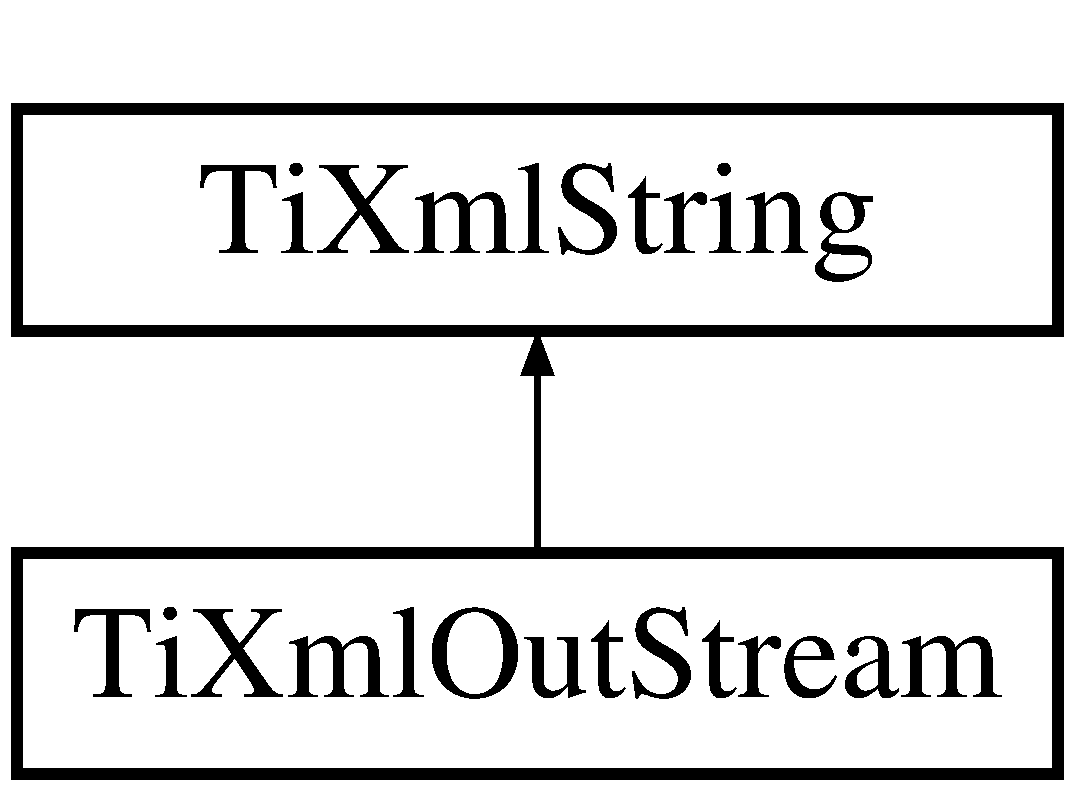
\includegraphics[height=2.000000cm]{classTiXmlString}
\end{center}
\end{figure}
\subsection*{Public Types}
\begin{DoxyCompactItemize}
\item 
\mbox{\label{classTiXmlString_abeb2c1893a04c17904f7c06546d0b971}} 
typedef size\+\_\+t {\bfseries size\+\_\+type}
\end{DoxyCompactItemize}
\subsection*{Public Member Functions}
\begin{DoxyCompactItemize}
\item 
\mbox{\label{classTiXmlString_ac80fe17693a438c9ab2591664743fcb6}} 
{\bfseries Ti\+Xml\+String} (const \textbf{ Ti\+Xml\+String} \&copy)
\item 
\mbox{\label{classTiXmlString_aa3b32bd2891a757c9f36c21db44c81d2}} 
T\+I\+X\+M\+L\+\_\+\+E\+X\+P\+L\+I\+C\+IT {\bfseries Ti\+Xml\+String} (const char $\ast$copy)
\item 
\mbox{\label{classTiXmlString_a4b17ea5c5db986f14827223dfa8f1547}} 
T\+I\+X\+M\+L\+\_\+\+E\+X\+P\+L\+I\+C\+IT {\bfseries Ti\+Xml\+String} (const char $\ast$str, size\+\_\+type len)
\item 
\mbox{\label{classTiXmlString_ae0bc6147afc0ec2aa0da3a3c0a8fcfb0}} 
\textbf{ Ti\+Xml\+String} \& {\bfseries operator=} (const char $\ast$copy)
\item 
\mbox{\label{classTiXmlString_ab1f1f5d3eceaa0f22d0a7e6055ea81b0}} 
\textbf{ Ti\+Xml\+String} \& {\bfseries operator=} (const \textbf{ Ti\+Xml\+String} \&copy)
\item 
\mbox{\label{classTiXmlString_ab56336ac2aa2a08d24a71eb9a2b502a5}} 
\textbf{ Ti\+Xml\+String} \& {\bfseries operator+=} (const char $\ast$suffix)
\item 
\mbox{\label{classTiXmlString_a6aa09d5240470b76d54ec709e04f8c13}} 
\textbf{ Ti\+Xml\+String} \& {\bfseries operator+=} (char single)
\item 
\mbox{\label{classTiXmlString_afdcae5ea2b4d9e194dc21226b817f417}} 
\textbf{ Ti\+Xml\+String} \& {\bfseries operator+=} (const \textbf{ Ti\+Xml\+String} \&suffix)
\item 
\mbox{\label{classTiXmlString_ae2bd36349215612ebcc3cb221c30bd3d}} 
const char $\ast$ {\bfseries c\+\_\+str} () const
\item 
\mbox{\label{classTiXmlString_a0e010e1737cfc3ee885b42875171b88e}} 
const char $\ast$ {\bfseries data} () const
\item 
\mbox{\label{classTiXmlString_a5db17f8314ffe2a89df0f0eb6c2a4bf5}} 
size\+\_\+type {\bfseries length} () const
\item 
\mbox{\label{classTiXmlString_a483d85103d2a3ba8c0831e205c832f33}} 
size\+\_\+type {\bfseries size} () const
\item 
\mbox{\label{classTiXmlString_a3139aafb0f0a8e26d1a4ed58a50f3678}} 
bool {\bfseries empty} () const
\item 
\mbox{\label{classTiXmlString_a0ca248f026e698f79b8aa4c9ab8e1571}} 
size\+\_\+type {\bfseries capacity} () const
\item 
\mbox{\label{classTiXmlString_a7f33c37f7dfde5193f02521d2a7af1db}} 
const char \& {\bfseries at} (size\+\_\+type index) const
\item 
\mbox{\label{classTiXmlString_a06e8c84831fc146610369405f4aa4200}} 
char \& {\bfseries operator[$\,$]} (size\+\_\+type index) const
\item 
\mbox{\label{classTiXmlString_a22fc54a23c5a0ab771331a25a769516e}} 
size\+\_\+type {\bfseries find} (char lookup) const
\item 
\mbox{\label{classTiXmlString_a2d66cfd6986faceda62ca62db553a921}} 
size\+\_\+type {\bfseries find} (char tofind, size\+\_\+type offset) const
\item 
\mbox{\label{classTiXmlString_ab20e06e4c666abf3bdbfb3a1191d4888}} 
void {\bfseries clear} ()
\item 
\mbox{\label{classTiXmlString_a88ecf9f0f00cb5c67b6b637958d7049c}} 
void {\bfseries reserve} (size\+\_\+type cap)
\item 
\mbox{\label{classTiXmlString_afe4cd3452ccd7cd8c8cac16e24ea28d7}} 
\textbf{ Ti\+Xml\+String} \& {\bfseries assign} (const char $\ast$str, size\+\_\+type len)
\item 
\mbox{\label{classTiXmlString_a717b00190c8acdee94816d2f4f20e75a}} 
\textbf{ Ti\+Xml\+String} \& {\bfseries append} (const char $\ast$str, size\+\_\+type len)
\item 
\mbox{\label{classTiXmlString_aa392cbc180752a79f007f4f9280c7762}} 
void {\bfseries swap} (\textbf{ Ti\+Xml\+String} \&other)
\end{DoxyCompactItemize}
\subsection*{Static Public Attributes}
\begin{DoxyCompactItemize}
\item 
\mbox{\label{classTiXmlString_a1aa6260982d3a63f0c822fe40fd7b37f}} 
static const size\+\_\+type {\bfseries npos}
\end{DoxyCompactItemize}


The documentation for this class was generated from the following file\+:\begin{DoxyCompactItemize}
\item 
tinystr.\+h\end{DoxyCompactItemize}

\section{Ti\+Xml\+Text Class Reference}
\label{classTiXmlText}\index{Ti\+Xml\+Text@{Ti\+Xml\+Text}}


X\+ML text.  




{\ttfamily \#include $<$tinyxml.\+h$>$}

Inheritance diagram for Ti\+Xml\+Text\+:\begin{figure}[H]
\begin{center}
\leavevmode
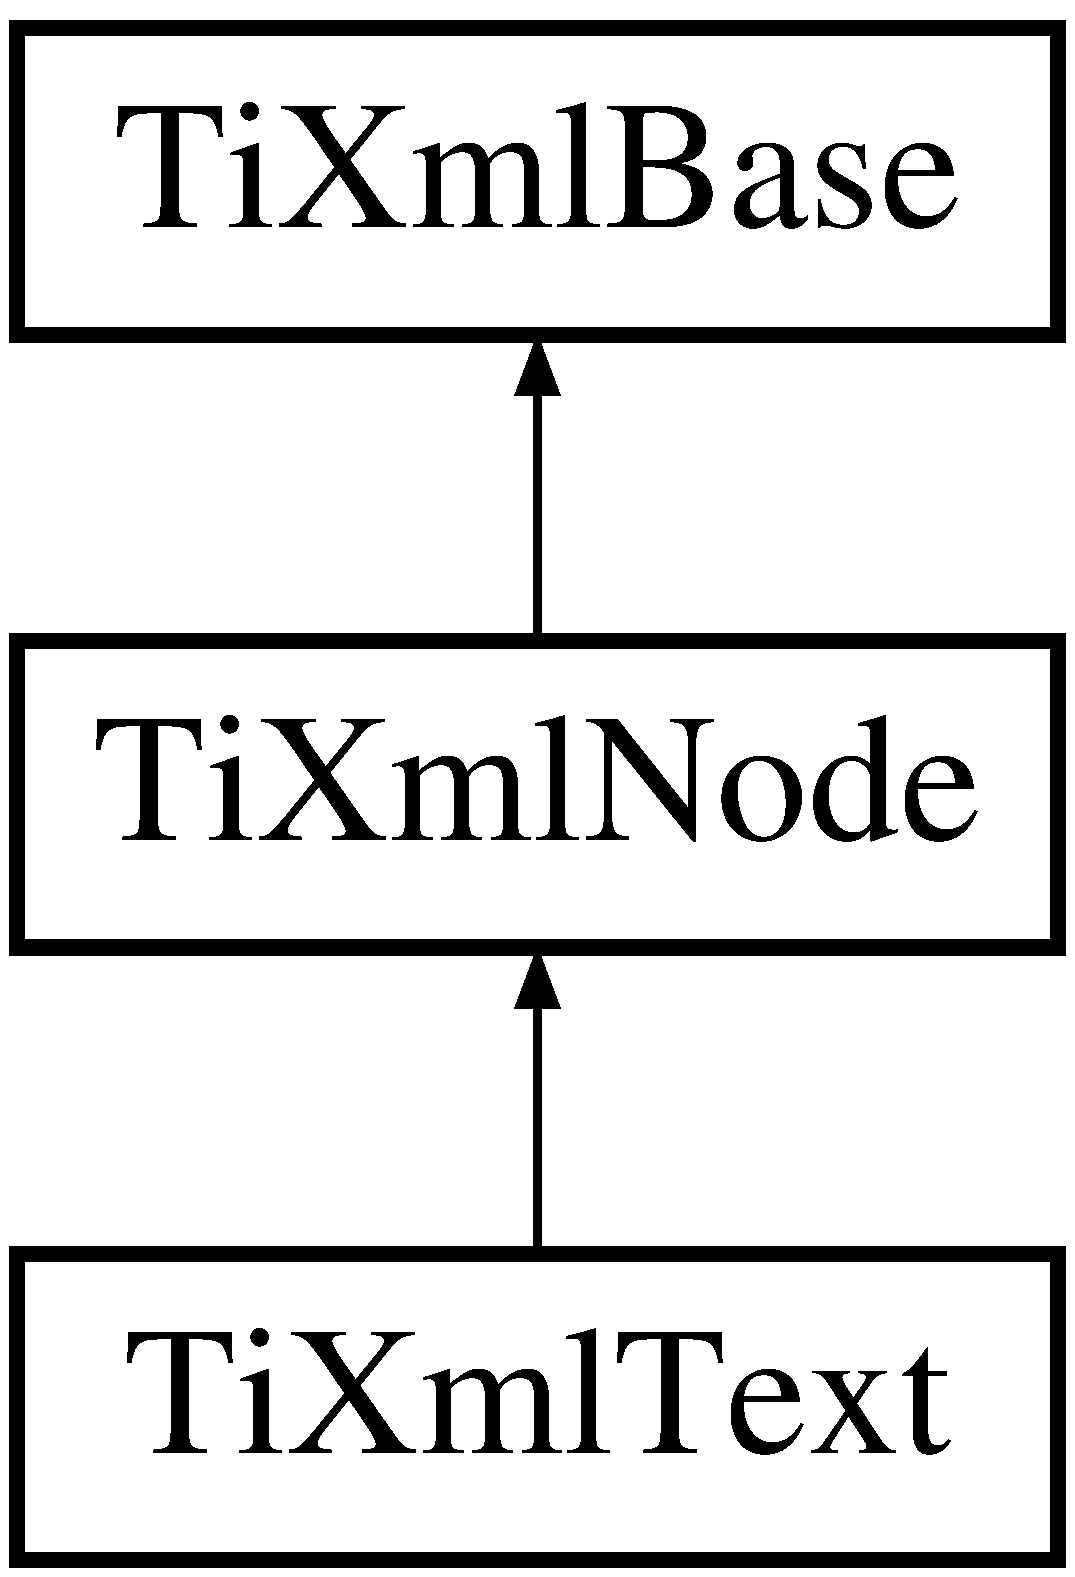
\includegraphics[height=3.000000cm]{classTiXmlText}
\end{center}
\end{figure}
\subsection*{Public Member Functions}
\begin{DoxyCompactItemize}
\item 
\textbf{ Ti\+Xml\+Text} (const char $\ast$init\+Value)
\begin{DoxyCompactList}\small\item\em Constructor for text element. \end{DoxyCompactList}\item 
\mbox{\label{classTiXmlText_a439792f6183a3d3fb6f2bc2b16fa5691}} 
\textbf{ Ti\+Xml\+Text} (const std\+::string \&init\+Value)
\begin{DoxyCompactList}\small\item\em Constructor. \end{DoxyCompactList}\item 
\mbox{\label{classTiXmlText_a8d2cc1b4af2208cbb0171cf20f6815d1}} 
{\bfseries Ti\+Xml\+Text} (const \textbf{ Ti\+Xml\+Text} \&copy)
\item 
\mbox{\label{classTiXmlText_af5f15d40d048cea7cab9d0eb4fd8a7d2}} 
void {\bfseries operator=} (const \textbf{ Ti\+Xml\+Text} \&base)
\item 
virtual void \textbf{ Print} (F\+I\+LE $\ast$cfile, int depth) const
\begin{DoxyCompactList}\small\item\em All Tiny\+Xml classes can print themselves to a filestream or the string class (\doxyref{Ti\+Xml\+String}{p.}{classTiXmlString} in non-\/\+S\+TL mode, std\+::string in S\+TL mode.) Either or both cfile and str can be null. \end{DoxyCompactList}\item 
\mbox{\label{classTiXmlText_aac1f4764d220ed6bf809b16dfcb6b45a}} 
bool \textbf{ C\+D\+A\+TA} () const
\begin{DoxyCompactList}\small\item\em Queries whether this represents text using a C\+D\+A\+TA section. \end{DoxyCompactList}\item 
\mbox{\label{classTiXmlText_acb17ff7c5d09b2c839393445a3de5ea9}} 
void \textbf{ Set\+C\+D\+A\+TA} (bool \+\_\+cdata)
\begin{DoxyCompactList}\small\item\em Turns on or off a C\+D\+A\+TA representation of text. \end{DoxyCompactList}\item 
\mbox{\label{classTiXmlText_a8d2dcfa41fc73d3e62dacc2fcf633819}} 
virtual const char $\ast$ {\bfseries Parse} (const char $\ast$p, \textbf{ Ti\+Xml\+Parsing\+Data} $\ast$data, Ti\+Xml\+Encoding encoding)
\item 
\mbox{\label{classTiXmlText_af8973cfd4ca00c5d934cb23e8aa0f5d5}} 
virtual const \textbf{ Ti\+Xml\+Text} $\ast$ \textbf{ To\+Text} () const
\begin{DoxyCompactList}\small\item\em Cast to a more defined type. Will return null not of the requested type. \end{DoxyCompactList}\item 
\mbox{\label{classTiXmlText_ae7c3a8fd3e4dbf6c0c4363a943d72f5b}} 
virtual \textbf{ Ti\+Xml\+Text} $\ast$ \textbf{ To\+Text} ()
\begin{DoxyCompactList}\small\item\em Cast to a more defined type. Will return null not of the requested type. \end{DoxyCompactList}\item 
\mbox{\label{classTiXmlText_af65964326eac4640bfb97d4622fa0de2}} 
virtual bool \textbf{ Accept} (\textbf{ Ti\+Xml\+Visitor} $\ast$content) const
\begin{DoxyCompactList}\small\item\em Walk the X\+ML tree visiting this node and all of its children. \end{DoxyCompactList}\end{DoxyCompactItemize}
\subsection*{Protected Member Functions}
\begin{DoxyCompactItemize}
\item 
\mbox{\label{classTiXmlText_a98a20d7a4f1c1478e25e34921be24bfe}} 
virtual \textbf{ Ti\+Xml\+Node} $\ast$ \textbf{ Clone} () const
\begin{DoxyCompactList}\small\item\em [internal use] Creates a new Element and returns it. \end{DoxyCompactList}\item 
\mbox{\label{classTiXmlText_a480b8e0ad6b7833a73ecf2191195c9b5}} 
void {\bfseries Copy\+To} (\textbf{ Ti\+Xml\+Text} $\ast$target) const
\item 
\mbox{\label{classTiXmlText_a0fd9005b279def46859b72f336b158da}} 
bool {\bfseries Blank} () const
\item 
\mbox{\label{classTiXmlText_ab0ad9f14fd41689ced26f21a5c8919b4}} 
virtual void {\bfseries Stream\+In} (std\+::istream $\ast$in, T\+I\+X\+M\+L\+\_\+\+S\+T\+R\+I\+NG $\ast$tag)
\end{DoxyCompactItemize}
\subsection*{Friends}
\begin{DoxyCompactItemize}
\item 
\mbox{\label{classTiXmlText_ab6592e32cb9132be517cc12a70564c4b}} 
class {\bfseries Ti\+Xml\+Element}
\end{DoxyCompactItemize}
\subsection*{Additional Inherited Members}


\subsection{Detailed Description}
X\+ML text. 

A text node can have 2 ways to output the next. \char`\"{}normal\char`\"{} output and C\+D\+A\+TA. It will default to the mode it was parsed from the X\+ML file and you generally want to leave it alone, but you can change the output mode with \doxyref{Set\+C\+D\+A\+T\+A()}{p.}{classTiXmlText_acb17ff7c5d09b2c839393445a3de5ea9} and query it with \doxyref{C\+D\+A\+T\+A()}{p.}{classTiXmlText_aac1f4764d220ed6bf809b16dfcb6b45a}. 

\subsection{Constructor \& Destructor Documentation}
\mbox{\label{classTiXmlText_af659e77c6b87d684827f35a8f4895960}} 
\index{Ti\+Xml\+Text@{Ti\+Xml\+Text}!Ti\+Xml\+Text@{Ti\+Xml\+Text}}
\index{Ti\+Xml\+Text@{Ti\+Xml\+Text}!Ti\+Xml\+Text@{Ti\+Xml\+Text}}
\subsubsection{Ti\+Xml\+Text()}
{\footnotesize\ttfamily Ti\+Xml\+Text\+::\+Ti\+Xml\+Text (\begin{DoxyParamCaption}\item[{const char $\ast$}]{init\+Value }\end{DoxyParamCaption})\hspace{0.3cm}{\ttfamily [inline]}}



Constructor for text element. 

By default, it is treated as normal, encoded text. If you want it be output as a C\+D\+A\+TA text element, set the parameter \+\_\+cdata to \textquotesingle{}true\textquotesingle{} 

References Ti\+Xml\+Element\+::\+Print(), and Ti\+Xml\+Node\+::\+Set\+Value().



\subsection{Member Function Documentation}
\mbox{\label{classTiXmlText_a75f6895906333894e2574cc8cf77ea79}} 
\index{Ti\+Xml\+Text@{Ti\+Xml\+Text}!Print@{Print}}
\index{Print@{Print}!Ti\+Xml\+Text@{Ti\+Xml\+Text}}
\subsubsection{Print()}
{\footnotesize\ttfamily void Ti\+Xml\+Text\+::\+Print (\begin{DoxyParamCaption}\item[{F\+I\+LE $\ast$}]{cfile,  }\item[{int}]{depth }\end{DoxyParamCaption}) const\hspace{0.3cm}{\ttfamily [virtual]}}



All Tiny\+Xml classes can print themselves to a filestream or the string class (\doxyref{Ti\+Xml\+String}{p.}{classTiXmlString} in non-\/\+S\+TL mode, std\+::string in S\+TL mode.) Either or both cfile and str can be null. 

This is a formatted print, and will insert tabs and newlines.

(For an unformatted stream, use the $<$$<$ operator.) 

Implements \textbf{ Ti\+Xml\+Base} \doxyref{}{p.}{classTiXmlBase_a0de56b3f2ef14c65091a3b916437b512}.



The documentation for this class was generated from the following files\+:\begin{DoxyCompactItemize}
\item 
tinyxml.\+h\item 
tinyxml.\+cc\item 
tinyxmlparser.\+cc\end{DoxyCompactItemize}

\section{Ti\+Xml\+Unknown Class Reference}
\label{classTiXmlUnknown}\index{Ti\+Xml\+Unknown@{Ti\+Xml\+Unknown}}


Any tag that tiny\+Xml doesn\textquotesingle{}t recognize is saved as an unknown.  




{\ttfamily \#include $<$tinyxml.\+h$>$}

Inheritance diagram for Ti\+Xml\+Unknown\+:\begin{figure}[H]
\begin{center}
\leavevmode
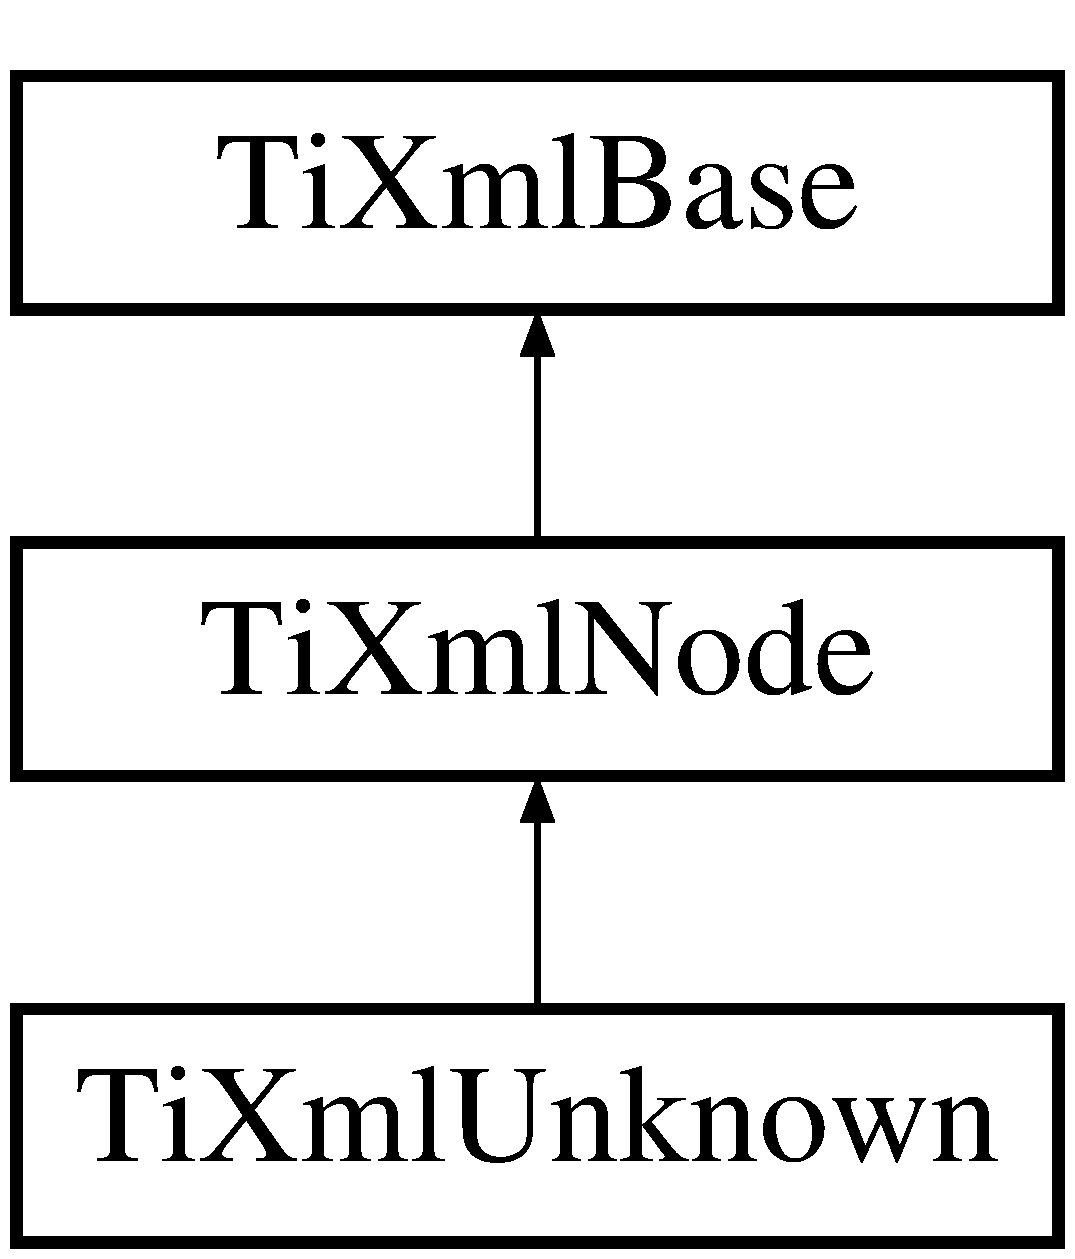
\includegraphics[height=3.000000cm]{classTiXmlUnknown}
\end{center}
\end{figure}
\subsection*{Public Member Functions}
\begin{DoxyCompactItemize}
\item 
\mbox{\label{classTiXmlUnknown_abe798ff4feea31474850c7f0de6bdf5e}} 
{\bfseries Ti\+Xml\+Unknown} (const \textbf{ Ti\+Xml\+Unknown} \&copy)
\item 
\mbox{\label{classTiXmlUnknown_a5097fe228cd5ad4edcdddf02c334fd83}} 
void {\bfseries operator=} (const \textbf{ Ti\+Xml\+Unknown} \&copy)
\item 
\mbox{\label{classTiXmlUnknown_a3dea7689de5b1931fd6657992948fde0}} 
virtual \textbf{ Ti\+Xml\+Node} $\ast$ \textbf{ Clone} () const
\begin{DoxyCompactList}\small\item\em Creates a copy of this Unknown and returns it. \end{DoxyCompactList}\item 
virtual void \textbf{ Print} (F\+I\+LE $\ast$cfile, int depth) const
\begin{DoxyCompactList}\small\item\em All Tiny\+Xml classes can print themselves to a filestream or the string class (\doxyref{Ti\+Xml\+String}{p.}{classTiXmlString} in non-\/\+S\+TL mode, std\+::string in S\+TL mode.) Either or both cfile and str can be null. \end{DoxyCompactList}\item 
\mbox{\label{classTiXmlUnknown_aa51c2694e4177b5f0b5429ee5a81b58d}} 
virtual const char $\ast$ {\bfseries Parse} (const char $\ast$p, \textbf{ Ti\+Xml\+Parsing\+Data} $\ast$data, Ti\+Xml\+Encoding encoding)
\item 
\mbox{\label{classTiXmlUnknown_a0d08dc16fc9ce16140ccaefbc35f6ea6}} 
virtual const \textbf{ Ti\+Xml\+Unknown} $\ast$ \textbf{ To\+Unknown} () const
\begin{DoxyCompactList}\small\item\em Cast to a more defined type. Will return null not of the requested type. \end{DoxyCompactList}\item 
\mbox{\label{classTiXmlUnknown_a67c9fd22940e8c47f706a72cdd2e332c}} 
virtual \textbf{ Ti\+Xml\+Unknown} $\ast$ \textbf{ To\+Unknown} ()
\begin{DoxyCompactList}\small\item\em Cast to a more defined type. Will return null not of the requested type. \end{DoxyCompactList}\item 
\mbox{\label{classTiXmlUnknown_aafdf1b2d4f561979c7907bad91004999}} 
virtual bool \textbf{ Accept} (\textbf{ Ti\+Xml\+Visitor} $\ast$content) const
\begin{DoxyCompactList}\small\item\em Walk the X\+ML tree visiting this node and all of its children. \end{DoxyCompactList}\end{DoxyCompactItemize}
\subsection*{Protected Member Functions}
\begin{DoxyCompactItemize}
\item 
\mbox{\label{classTiXmlUnknown_afeb334446bcbe13ce15131e1629712be}} 
void {\bfseries Copy\+To} (\textbf{ Ti\+Xml\+Unknown} $\ast$target) const
\item 
\mbox{\label{classTiXmlUnknown_ad3f8fcc1efe364ddd8f43ef9a1046300}} 
virtual void {\bfseries Stream\+In} (std\+::istream $\ast$in, T\+I\+X\+M\+L\+\_\+\+S\+T\+R\+I\+NG $\ast$tag)
\end{DoxyCompactItemize}
\subsection*{Additional Inherited Members}


\subsection{Detailed Description}
Any tag that tiny\+Xml doesn\textquotesingle{}t recognize is saved as an unknown. 

It is a tag of text, but should not be modified. It will be written back to the X\+ML, unchanged, when the file is saved.

D\+TD tags get thrown into Ti\+Xml\+Unknowns. 

\subsection{Member Function Documentation}
\mbox{\label{classTiXmlUnknown_a5793fbc48ab3419783c0e866ca2d334e}} 
\index{Ti\+Xml\+Unknown@{Ti\+Xml\+Unknown}!Print@{Print}}
\index{Print@{Print}!Ti\+Xml\+Unknown@{Ti\+Xml\+Unknown}}
\subsubsection{Print()}
{\footnotesize\ttfamily void Ti\+Xml\+Unknown\+::\+Print (\begin{DoxyParamCaption}\item[{F\+I\+LE $\ast$}]{cfile,  }\item[{int}]{depth }\end{DoxyParamCaption}) const\hspace{0.3cm}{\ttfamily [virtual]}}



All Tiny\+Xml classes can print themselves to a filestream or the string class (\doxyref{Ti\+Xml\+String}{p.}{classTiXmlString} in non-\/\+S\+TL mode, std\+::string in S\+TL mode.) Either or both cfile and str can be null. 

This is a formatted print, and will insert tabs and newlines.

(For an unformatted stream, use the $<$$<$ operator.) 

Implements \textbf{ Ti\+Xml\+Base} \doxyref{}{p.}{classTiXmlBase_a0de56b3f2ef14c65091a3b916437b512}.



The documentation for this class was generated from the following files\+:\begin{DoxyCompactItemize}
\item 
tinyxml.\+h\item 
tinyxml.\+cc\item 
tinyxmlparser.\+cc\end{DoxyCompactItemize}

\section{Ti\+Xml\+Visitor Class Reference}
\label{classTiXmlVisitor}\index{Ti\+Xml\+Visitor@{Ti\+Xml\+Visitor}}


If you call the Accept() method, it requires being passed a \doxyref{Ti\+Xml\+Visitor}{p.}{classTiXmlVisitor} class to handle callbacks.  




{\ttfamily \#include $<$tinyxml.\+h$>$}

Inheritance diagram for Ti\+Xml\+Visitor\+:\begin{figure}[H]
\begin{center}
\leavevmode
\includegraphics[height=2.000000cm]{classTiXmlVisitor}
\end{center}
\end{figure}
\subsection*{Public Member Functions}
\begin{DoxyCompactItemize}
\item 
\mbox{\label{classTiXmlVisitor_a07baecb52dd7d8716ae2a48ad0956ee0}} 
virtual bool \textbf{ Visit\+Enter} (const \textbf{ Ti\+Xml\+Document} \&)
\begin{DoxyCompactList}\small\item\em Visit a document. \end{DoxyCompactList}\item 
\mbox{\label{classTiXmlVisitor_aa0ade4f27087447e93974e975c3246ad}} 
virtual bool \textbf{ Visit\+Exit} (const \textbf{ Ti\+Xml\+Document} \&)
\begin{DoxyCompactList}\small\item\em Visit a document. \end{DoxyCompactList}\item 
\mbox{\label{classTiXmlVisitor_af6c6178ffa517bbdba95d70490875fff}} 
virtual bool \textbf{ Visit\+Enter} (const \textbf{ Ti\+Xml\+Element} \&, const \textbf{ Ti\+Xml\+Attribute} $\ast$)
\begin{DoxyCompactList}\small\item\em Visit an element. \end{DoxyCompactList}\item 
\mbox{\label{classTiXmlVisitor_aec2b1f8116226d52f3a1b95dafd3a32c}} 
virtual bool \textbf{ Visit\+Exit} (const \textbf{ Ti\+Xml\+Element} \&)
\begin{DoxyCompactList}\small\item\em Visit an element. \end{DoxyCompactList}\item 
\mbox{\label{classTiXmlVisitor_afad71c71ce6473fb9b4b64cd92de4a19}} 
virtual bool \textbf{ Visit} (const \textbf{ Ti\+Xml\+Declaration} \&)
\begin{DoxyCompactList}\small\item\em Visit a declaration. \end{DoxyCompactList}\item 
\mbox{\label{classTiXmlVisitor_a399b8ebca5cd14664974a32d2ce029e5}} 
virtual bool \textbf{ Visit} (const \textbf{ Ti\+Xml\+Text} \&)
\begin{DoxyCompactList}\small\item\em Visit a text node. \end{DoxyCompactList}\item 
\mbox{\label{classTiXmlVisitor_a53a60e7a528627b31af3161972cc7fa2}} 
virtual bool \textbf{ Visit} (const \textbf{ Ti\+Xml\+Comment} \&)
\begin{DoxyCompactList}\small\item\em Visit a comment node. \end{DoxyCompactList}\item 
\mbox{\label{classTiXmlVisitor_a7e284d607d275c51dac1adb58159ce28}} 
virtual bool \textbf{ Visit} (const \textbf{ Ti\+Xml\+Unknown} \&)
\begin{DoxyCompactList}\small\item\em Visit an unknow node. \end{DoxyCompactList}\end{DoxyCompactItemize}


\subsection{Detailed Description}
If you call the Accept() method, it requires being passed a \doxyref{Ti\+Xml\+Visitor}{p.}{classTiXmlVisitor} class to handle callbacks. 

For nodes that contain other nodes (Document, Element) you will get called with a Visit\+Enter/\+Visit\+Exit pair. Nodes that are always leaves are simple called with \doxyref{Visit()}{p.}{classTiXmlVisitor_afad71c71ce6473fb9b4b64cd92de4a19}.

If you return \textquotesingle{}true\textquotesingle{} from a Visit method, recursive parsing will continue. If you return false, {\bfseries no children of this node or its sibilings} will be Visited.

All flavors of Visit methods have a default implementation that returns \textquotesingle{}true\textquotesingle{} (continue visiting). You need to only override methods that are interesting to you.

Generally Accept() is called on the \doxyref{Ti\+Xml\+Document}{p.}{classTiXmlDocument}, although all nodes suppert Visiting.

You should never change the document from a callback.

\begin{DoxySeeAlso}{See also}
\doxyref{Ti\+Xml\+Node\+::\+Accept()}{p.}{classTiXmlNode_acc0f88b7462c6cb73809d410a4f5bb86} 
\end{DoxySeeAlso}


The documentation for this class was generated from the following file\+:\begin{DoxyCompactItemize}
\item 
tinyxml.\+h\end{DoxyCompactItemize}

\section{marlin\+:\+:Tokenizer Class Reference}
\label{classmarlin_1_1Tokenizer}\index{marlin\+::\+Tokenizer@{marlin\+::\+Tokenizer}}


Helper class for \doxyref{Logical\+Expressions}{p.}{classmarlin_1_1LogicalExpressions} that splits the expression into subexpressions -\/ needs to be apllied iteratively.  




{\ttfamily \#include $<$Logical\+Expressions.\+h$>$}

\subsection*{Public Member Functions}
\begin{DoxyCompactItemize}
\item 
\mbox{\label{classmarlin_1_1Tokenizer_a2eea3b78d9b7279ca27efcc326425272}} 
{\bfseries Tokenizer} (std\+::vector$<$ \textbf{ Expression} $>$ \&tokens)
\item 
\mbox{\label{classmarlin_1_1Tokenizer_a55d4e451533ddf49c09ecda3ea1b39c5}} 
void \textbf{ operator()} (const char \&c)
\begin{DoxyCompactList}\small\item\em Save the current character and change state if necessary. \end{DoxyCompactList}\item 
\mbox{\label{classmarlin_1_1Tokenizer_a600fd3127f42e18163286b5d71d53bf5}} 
std\+::vector$<$ \textbf{ Expression} $>$ \& {\bfseries result} ()
\end{DoxyCompactItemize}


\subsection{Detailed Description}
Helper class for \doxyref{Logical\+Expressions}{p.}{classmarlin_1_1LogicalExpressions} that splits the expression into subexpressions -\/ needs to be apllied iteratively. 

The documentation for this class was generated from the following file\+:\begin{DoxyCompactItemize}
\item 
Logical\+Expressions.\+h\end{DoxyCompactItemize}

\section{marlin\+:\+:Track\+Resolution Struct Reference}
\label{structmarlin_1_1TrackResolution}\index{marlin\+::\+Track\+Resolution@{marlin\+::\+Track\+Resolution}}


Small helper class to store tracker resolutions for a polar angle range.  




{\ttfamily \#include $<$Simple\+Track\+Smearer.\+h$>$}

\subsection*{Public Member Functions}
\begin{DoxyCompactItemize}
\item 
\mbox{\label{structmarlin_1_1TrackResolution_a6bef466a2db2b60477ed42c4f4c126f8}} 
{\bfseries Track\+Resolution} (float d\+PP, float th\+Min, float th\+Max)
\end{DoxyCompactItemize}
\subsection*{Public Attributes}
\begin{DoxyCompactItemize}
\item 
\mbox{\label{structmarlin_1_1TrackResolution_a10a3075f66af77eece3ce39503a458ab}} 
float {\bfseries D\+PP}
\item 
\mbox{\label{structmarlin_1_1TrackResolution_a4bdb57d219546a2766ad1abe521a6085}} 
float {\bfseries Th\+Min}
\item 
\mbox{\label{structmarlin_1_1TrackResolution_aefc2cf39af85063f0d3fd79512baaff7}} 
float {\bfseries Th\+Max}
\end{DoxyCompactItemize}


\subsection{Detailed Description}
Small helper class to store tracker resolutions for a polar angle range. 

\begin{DoxyAuthor}{Author}
F. Gaede, D\+E\+SY 
\end{DoxyAuthor}
\begin{DoxyVersion}{Version}

\end{DoxyVersion}
\begin{DoxyParagraph}{Id}
\doxyref{Simple\+Track\+Smearer.\+h}{p.}{SimpleTrackSmearer_8h_source},v 1.\+2 2005-\/10-\/11 12\+:56\+:28 gaede Exp 
\end{DoxyParagraph}


The documentation for this struct was generated from the following file\+:\begin{DoxyCompactItemize}
\item 
Simple\+Track\+Smearer.\+h\end{DoxyCompactItemize}

\section{marlin\+:\+:concurrency\+:\+:Worker$<$ IN, O\+UT $>$ Class Template Reference}
\label{classmarlin_1_1concurrency_1_1Worker}\index{marlin\+::concurrency\+::\+Worker$<$ I\+N, O\+U\+T $>$@{marlin\+::concurrency\+::\+Worker$<$ I\+N, O\+U\+T $>$}}


\doxyref{Worker}{p.}{classmarlin_1_1concurrency_1_1Worker} class.  




{\ttfamily \#include $<$Worker.\+h$>$}

\subsection*{Public Types}
\begin{DoxyCompactItemize}
\item 
\mbox{\label{classmarlin_1_1concurrency_1_1Worker_ad3b134a2dea5b6bb92d0c47d4a4233f3}} 
using {\bfseries Input} = IN
\item 
\mbox{\label{classmarlin_1_1concurrency_1_1Worker_a1dfa1d2702d5a59e845a3f2737e8bd1e}} 
using {\bfseries Output} = O\+UT
\item 
\mbox{\label{classmarlin_1_1concurrency_1_1Worker_aa6aac3bbd7ac3f3754393f0b59047f83}} 
using {\bfseries Pool} = \textbf{ Thread\+Pool}$<$ IN, O\+UT $>$
\item 
\mbox{\label{classmarlin_1_1concurrency_1_1Worker_ad02207eff99facf7aca5021bba9c1f31}} 
using {\bfseries Impl} = \textbf{ Worker\+Base}$<$ IN, O\+UT $>$
\end{DoxyCompactItemize}
\subsection*{Public Member Functions}
\begin{DoxyCompactItemize}
\item 
\mbox{\label{classmarlin_1_1concurrency_1_1Worker_a2a4d3a6bdd4ee57f37b20f589e6d8708}} 
{\bfseries Worker} (const \textbf{ Worker} \&)=delete
\item 
\mbox{\label{classmarlin_1_1concurrency_1_1Worker_a38d1b9e8f4525a052a2a3b65f8af6348}} 
{\bfseries Worker} (\textbf{ Worker} \&\&)=delete
\item 
\mbox{\label{classmarlin_1_1concurrency_1_1Worker_a5a2fb98247af1af2c2344793afabed57}} 
\textbf{ Worker} \& {\bfseries operator=} (const \textbf{ Worker} \&)=delete
\item 
\mbox{\label{classmarlin_1_1concurrency_1_1Worker_a781f94ec24294e23f8f71d6a29175b7f}} 
\textbf{ Worker} \& {\bfseries operator=} (\textbf{ Worker} \&\&)=delete
\item 
{\footnotesize template$<$typename I\+M\+PL , class  = typename std\+::enable\+\_\+if$<$std\+::is\+\_\+base\+\_\+of$<$\+Impl,\+I\+M\+P\+L$>$\+::value$>$\+::type$>$ }\\\textbf{ Worker} (\textbf{ Pool} \&pool, std\+::unique\+\_\+ptr$<$ I\+M\+PL $>$ impl)
\begin{DoxyCompactList}\small\item\em Constructor. \end{DoxyCompactList}\item 
\mbox{\label{classmarlin_1_1concurrency_1_1Worker_a63b4bc300b68289dc54df66d950a9e79}} 
void \textbf{ start} ()
\begin{DoxyCompactList}\small\item\em Start the worker thread. \end{DoxyCompactList}\item 
\mbox{\label{classmarlin_1_1concurrency_1_1Worker_ac84802b22f04965da47146326c97d73c}} 
void \textbf{ run} ()
\begin{DoxyCompactList}\small\item\em The method executing in the worker thread. \end{DoxyCompactList}\item 
void \textbf{ stop} ()
\begin{DoxyCompactList}\small\item\em Switch ON the stop flag, requesting the worker thread to stop. \end{DoxyCompactList}\item 
\mbox{\label{classmarlin_1_1concurrency_1_1Worker_ad898c2f7fdcb8510289f95884cd99805}} 
bool \textbf{ running} () const
\begin{DoxyCompactList}\small\item\em Whether the worker thread is currently running. \end{DoxyCompactList}\item 
\mbox{\label{classmarlin_1_1concurrency_1_1Worker_a2e9825175d9c6ac7a4cd7708f088c304}} 
bool \textbf{ waiting} () const
\begin{DoxyCompactList}\small\item\em Whether the worker is waiting. \end{DoxyCompactList}\item 
\mbox{\label{classmarlin_1_1concurrency_1_1Worker_ab516e3e2e156dc06a3cda177fee68eb4}} 
void \textbf{ join} ()
\begin{DoxyCompactList}\small\item\em Join the worker thread. \end{DoxyCompactList}\end{DoxyCompactItemize}


\subsection{Detailed Description}
\subsubsection*{template$<$typename IN, typename O\+UT$>$\newline
class marlin\+::concurrency\+::\+Worker$<$ I\+N, O\+U\+T $>$}

\doxyref{Worker}{p.}{classmarlin_1_1concurrency_1_1Worker} class. 

\subsection{Constructor \& Destructor Documentation}
\mbox{\label{classmarlin_1_1concurrency_1_1Worker_a475a7f182663aa74a3d2967216fa75e1}} 
\index{marlin\+::concurrency\+::\+Worker@{marlin\+::concurrency\+::\+Worker}!Worker@{Worker}}
\index{Worker@{Worker}!marlin\+::concurrency\+::\+Worker@{marlin\+::concurrency\+::\+Worker}}
\subsubsection{Worker()}
{\footnotesize\ttfamily template$<$typename IN , typename O\+UT $>$ \\
template$<$typename I\+M\+PL , class $>$ \\
\textbf{ marlin\+::concurrency\+::\+Worker}$<$ IN, O\+UT $>$\+::\textbf{ Worker} (\begin{DoxyParamCaption}\item[{\textbf{ Pool} \&}]{pool,  }\item[{std\+::unique\+\_\+ptr$<$ I\+M\+PL $>$}]{impl }\end{DoxyParamCaption})\hspace{0.3cm}{\ttfamily [inline]}}



Constructor. 


\begin{DoxyParams}{Parameters}
{\em pool} & the parent thread pool \\
\hline
{\em impl} & the worker implementation consuming IN data, producing O\+UT data \\
\hline
\end{DoxyParams}


\subsection{Member Function Documentation}
\mbox{\label{classmarlin_1_1concurrency_1_1Worker_ae61da10a43d96508ed876c467693c581}} 
\index{marlin\+::concurrency\+::\+Worker@{marlin\+::concurrency\+::\+Worker}!stop@{stop}}
\index{stop@{stop}!marlin\+::concurrency\+::\+Worker@{marlin\+::concurrency\+::\+Worker}}
\subsubsection{stop()}
{\footnotesize\ttfamily template$<$typename IN , typename O\+UT $>$ \\
void \textbf{ marlin\+::concurrency\+::\+Worker}$<$ IN, O\+UT $>$\+::stop (\begin{DoxyParamCaption}{ }\end{DoxyParamCaption})\hspace{0.3cm}{\ttfamily [inline]}}



Switch ON the stop flag, requesting the worker thread to stop. 

No join operation is done here. See \doxyref{join()}{p.}{classmarlin_1_1concurrency_1_1Worker_ab516e3e2e156dc06a3cda177fee68eb4} method 

The documentation for this class was generated from the following files\+:\begin{DoxyCompactItemize}
\item 
Thread\+Pool.\+h\item 
Worker.\+h\end{DoxyCompactItemize}

\section{marlin\+:\+:concurrency\+:\+:Worker\+Base$<$ IN, O\+UT $>$ Class Template Reference}
\label{classmarlin_1_1concurrency_1_1WorkerBase}\index{marlin\+::concurrency\+::\+Worker\+Base$<$ I\+N, O\+U\+T $>$@{marlin\+::concurrency\+::\+Worker\+Base$<$ I\+N, O\+U\+T $>$}}


\doxyref{Worker\+Base}{p.}{classmarlin_1_1concurrency_1_1WorkerBase} class Base class to implement processing of task data (so called queued-\/element) pushed in a thread pool.  




{\ttfamily \#include $<$Worker.\+h$>$}

\subsection*{Public Types}
\begin{DoxyCompactItemize}
\item 
\mbox{\label{classmarlin_1_1concurrency_1_1WorkerBase_aaed18cd6efbee237183378738b92d5b6}} 
using {\bfseries Input} = IN
\item 
\mbox{\label{classmarlin_1_1concurrency_1_1WorkerBase_abf64f64e9e63fbed57ba72174e634c59}} 
using {\bfseries Output} = O\+UT
\end{DoxyCompactItemize}
\subsection*{Public Member Functions}
\begin{DoxyCompactItemize}
\item 
virtual O\+UT \textbf{ process} (IN \&\&data)=0
\begin{DoxyCompactList}\small\item\em Process a single queued data taken form the thread pool. \end{DoxyCompactList}\end{DoxyCompactItemize}
\subsection*{Protected Member Functions}
\begin{DoxyCompactItemize}
\item 
void \textbf{ process\+Element} (\textbf{ Queue\+Element}$<$ IN, O\+UT $>$ \&element)
\begin{DoxyCompactList}\small\item\em Process queued element from the thread pool. \end{DoxyCompactList}\end{DoxyCompactItemize}
\subsection*{Friends}
\begin{DoxyCompactItemize}
\item 
\mbox{\label{classmarlin_1_1concurrency_1_1WorkerBase_a491b906d2052cbe1c394c75e0e2d72a5}} 
class {\bfseries Worker$<$ I\+N, O\+U\+T $>$}
\end{DoxyCompactItemize}


\subsection{Detailed Description}
\subsubsection*{template$<$typename IN, typename O\+UT$>$\newline
class marlin\+::concurrency\+::\+Worker\+Base$<$ I\+N, O\+U\+T $>$}

\doxyref{Worker\+Base}{p.}{classmarlin_1_1concurrency_1_1WorkerBase} class Base class to implement processing of task data (so called queued-\/element) pushed in a thread pool. 

The IN and O\+UT types must be movable. See also specialization for void IN and O\+UT types 

\subsection{Member Function Documentation}
\mbox{\label{classmarlin_1_1concurrency_1_1WorkerBase_a543763db083b1c4cf846a3e1434ada11}} 
\index{marlin\+::concurrency\+::\+Worker\+Base@{marlin\+::concurrency\+::\+Worker\+Base}!process@{process}}
\index{process@{process}!marlin\+::concurrency\+::\+Worker\+Base@{marlin\+::concurrency\+::\+Worker\+Base}}
\subsubsection{process()}
{\footnotesize\ttfamily template$<$typename IN, typename O\+UT$>$ \\
virtual O\+UT \textbf{ marlin\+::concurrency\+::\+Worker\+Base}$<$ IN, O\+UT $>$\+::process (\begin{DoxyParamCaption}\item[{IN \&\&}]{data }\end{DoxyParamCaption})\hspace{0.3cm}{\ttfamily [pure virtual]}}



Process a single queued data taken form the thread pool. 


\begin{DoxyParams}{Parameters}
{\em data} & the data value to process \\
\hline
\end{DoxyParams}


Referenced by marlin\+::concurrency\+::\+Worker\+Base$<$ P\+E\+P\+Scheduler\+::\+Input\+Type, P\+E\+P\+Scheduler\+::\+Output\+Type $>$\+::process\+Element().

\mbox{\label{classmarlin_1_1concurrency_1_1WorkerBase_ad426c1a9d78e564385a48293ef6c0ae7}} 
\index{marlin\+::concurrency\+::\+Worker\+Base@{marlin\+::concurrency\+::\+Worker\+Base}!process\+Element@{process\+Element}}
\index{process\+Element@{process\+Element}!marlin\+::concurrency\+::\+Worker\+Base@{marlin\+::concurrency\+::\+Worker\+Base}}
\subsubsection{process\+Element()}
{\footnotesize\ttfamily template$<$typename IN , typename O\+UT $>$ \\
void \textbf{ marlin\+::concurrency\+::\+Worker\+Base}$<$ IN, O\+UT $>$\+::process\+Element (\begin{DoxyParamCaption}\item[{\textbf{ Queue\+Element}$<$ IN, O\+UT $>$ \&}]{element }\end{DoxyParamCaption})\hspace{0.3cm}{\ttfamily [inline]}, {\ttfamily [protected]}}



Process queued element from the thread pool. 


\begin{DoxyParams}{Parameters}
{\em element} & a thread pool queued element \\
\hline
\end{DoxyParams}


Referenced by marlin\+::concurrency\+::\+Worker\+Base$<$ P\+E\+P\+Scheduler\+::\+Input\+Type, P\+E\+P\+Scheduler\+::\+Output\+Type $>$\+::process\+Element().



The documentation for this class was generated from the following file\+:\begin{DoxyCompactItemize}
\item 
Worker.\+h\end{DoxyCompactItemize}

\section{marlin\+:\+:concurrency\+:\+:Worker\+Base$<$ IN, void $>$ Class Template Reference}
\label{classmarlin_1_1concurrency_1_1WorkerBase_3_01IN_00_01void_01_4}\index{marlin\+::concurrency\+::\+Worker\+Base$<$ I\+N, void $>$@{marlin\+::concurrency\+::\+Worker\+Base$<$ I\+N, void $>$}}
\subsection*{Public Member Functions}
\begin{DoxyCompactItemize}
\item 
\mbox{\label{classmarlin_1_1concurrency_1_1WorkerBase_3_01IN_00_01void_01_4_ad35e6d3233031ccdfda2106539c87070}} 
virtual void {\bfseries process} (IN \&\&data)=0
\end{DoxyCompactItemize}
\subsection*{Protected Member Functions}
\begin{DoxyCompactItemize}
\item 
\mbox{\label{classmarlin_1_1concurrency_1_1WorkerBase_3_01IN_00_01void_01_4_a72188e60c2606807fcf9d8c03fa52182}} 
void {\bfseries process\+Element} (\textbf{ Queue\+Element}$<$ IN, void $>$ \&element)
\end{DoxyCompactItemize}
\subsection*{Friends}
\begin{DoxyCompactItemize}
\item 
\mbox{\label{classmarlin_1_1concurrency_1_1WorkerBase_3_01IN_00_01void_01_4_add3f4af0b28490976419290c6ee4691a}} 
class {\bfseries Worker$<$ I\+N, void $>$}
\end{DoxyCompactItemize}


The documentation for this class was generated from the following file\+:\begin{DoxyCompactItemize}
\item 
Worker.\+h\end{DoxyCompactItemize}

\section{marlin\+:\+:concurrency\+:\+:Worker\+Base$<$ void, O\+UT $>$ Class Template Reference}
\label{classmarlin_1_1concurrency_1_1WorkerBase_3_01void_00_01OUT_01_4}\index{marlin\+::concurrency\+::\+Worker\+Base$<$ void, O\+U\+T $>$@{marlin\+::concurrency\+::\+Worker\+Base$<$ void, O\+U\+T $>$}}
\subsection*{Public Member Functions}
\begin{DoxyCompactItemize}
\item 
\mbox{\label{classmarlin_1_1concurrency_1_1WorkerBase_3_01void_00_01OUT_01_4_a625081bfd8f7e3f1533a8db20324a1a8}} 
virtual O\+UT {\bfseries process} ()=0
\end{DoxyCompactItemize}
\subsection*{Protected Member Functions}
\begin{DoxyCompactItemize}
\item 
\mbox{\label{classmarlin_1_1concurrency_1_1WorkerBase_3_01void_00_01OUT_01_4_a42e0441da0a00b2dcda52ebf1c207f51}} 
void {\bfseries process\+Element} (\textbf{ Queue\+Element}$<$ void, O\+UT $>$ \&element)
\end{DoxyCompactItemize}
\subsection*{Friends}
\begin{DoxyCompactItemize}
\item 
\mbox{\label{classmarlin_1_1concurrency_1_1WorkerBase_3_01void_00_01OUT_01_4_a8232f4ec8f7f38b86d1a1487c8a974cf}} 
class {\bfseries Worker$<$ void, O\+U\+T $>$}
\end{DoxyCompactItemize}


The documentation for this class was generated from the following file\+:\begin{DoxyCompactItemize}
\item 
Worker.\+h\end{DoxyCompactItemize}

\section{marlin\+:\+:concurrency\+:\+:Worker\+Base$<$ void, void $>$ Class Template Reference}
\label{classmarlin_1_1concurrency_1_1WorkerBase_3_01void_00_01void_01_4}\index{marlin\+::concurrency\+::\+Worker\+Base$<$ void, void $>$@{marlin\+::concurrency\+::\+Worker\+Base$<$ void, void $>$}}
\subsection*{Public Member Functions}
\begin{DoxyCompactItemize}
\item 
\mbox{\label{classmarlin_1_1concurrency_1_1WorkerBase_3_01void_00_01void_01_4_a32fbcb5ee5fedf59bf35b6da99c0a7f9}} 
virtual void {\bfseries process} ()=0
\end{DoxyCompactItemize}
\subsection*{Protected Member Functions}
\begin{DoxyCompactItemize}
\item 
\mbox{\label{classmarlin_1_1concurrency_1_1WorkerBase_3_01void_00_01void_01_4_aa1c4e4311d209d6faafc31763595c7de}} 
void {\bfseries process\+Element} (\textbf{ Queue\+Element}$<$ void, void $>$ \&element)
\end{DoxyCompactItemize}
\subsection*{Friends}
\begin{DoxyCompactItemize}
\item 
\mbox{\label{classmarlin_1_1concurrency_1_1WorkerBase_3_01void_00_01void_01_4_ae8398d4a0c34bf21dc4d22748367d6d6}} 
class {\bfseries Worker$<$ void, void $>$}
\end{DoxyCompactItemize}


The documentation for this class was generated from the following file\+:\begin{DoxyCompactItemize}
\item 
Worker.\+h\end{DoxyCompactItemize}

\section{marlin\+:\+:concurrency\+:\+:Worker\+Output Struct Reference}
\label{structmarlin_1_1concurrency_1_1WorkerOutput}\index{marlin\+::concurrency\+::\+Worker\+Output@{marlin\+::concurrency\+::\+Worker\+Output}}


\doxyref{Worker\+Output}{p.}{structmarlin_1_1concurrency_1_1WorkerOutput} struct Stores the output of a processor sequence call.  




{\ttfamily \#include $<$P\+E\+P\+Scheduler.\+h$>$}

\subsection*{Public Attributes}
\begin{DoxyCompactItemize}
\item 
std\+::shared\+\_\+ptr$<$ E\+V\+E\+N\+T\+::\+L\+C\+Event $>$ \textbf{ \+\_\+event} \{nullptr\}
\begin{DoxyCompactList}\small\item\em $<$ The input event \end{DoxyCompactList}\item 
\mbox{\label{structmarlin_1_1concurrency_1_1WorkerOutput_a4b6826b26bfc1f5bdd5d1efa624e124e}} 
std\+::exception\+\_\+ptr {\bfseries \+\_\+exception} \{nullptr\}
\end{DoxyCompactItemize}


\subsection{Detailed Description}
\doxyref{Worker\+Output}{p.}{structmarlin_1_1concurrency_1_1WorkerOutput} struct Stores the output of a processor sequence call. 

\subsection{Member Data Documentation}
\mbox{\label{structmarlin_1_1concurrency_1_1WorkerOutput_a502688581a224c4dcbfcd131b0b96f94}} 
\index{marlin\+::concurrency\+::\+Worker\+Output@{marlin\+::concurrency\+::\+Worker\+Output}!\+\_\+event@{\+\_\+event}}
\index{\+\_\+event@{\+\_\+event}!marlin\+::concurrency\+::\+Worker\+Output@{marlin\+::concurrency\+::\+Worker\+Output}}
\subsubsection{\+\_\+event}
{\footnotesize\ttfamily std\+::shared\+\_\+ptr$<$E\+V\+E\+N\+T\+::\+L\+C\+Event$>$ marlin\+::concurrency\+::\+Worker\+Output\+::\+\_\+event \{nullptr\}}



$<$ The input event 

An exception potential throw in the worker thread 

The documentation for this struct was generated from the following file\+:\begin{DoxyCompactItemize}
\item 
P\+E\+P\+Scheduler.\+h\end{DoxyCompactItemize}

\section{marlin\+:\+:X\+M\+L\+Parser Class Reference}
\label{classmarlin_1_1XMLParser}\index{marlin\+::\+X\+M\+L\+Parser@{marlin\+::\+X\+M\+L\+Parser}}


X\+ML parser for Marlin steering files.  




{\ttfamily \#include $<$X\+M\+L\+Parser.\+h$>$}

Inheritance diagram for marlin\+:\+:X\+M\+L\+Parser\+:\begin{figure}[H]
\begin{center}
\leavevmode
\includegraphics[height=2.000000cm]{classmarlin_1_1XMLParser}
\end{center}
\end{figure}
\subsection*{Classes}
\begin{DoxyCompactItemize}
\item 
class \textbf{ L\+C\+Tokenizer}
\begin{DoxyCompactList}\small\item\em Helper class for \doxyref{X\+M\+L\+Parser}{p.}{classmarlin_1_1XMLParser}. \end{DoxyCompactList}\end{DoxyCompactItemize}
\subsection*{Public Member Functions}
\begin{DoxyCompactItemize}
\item 
\mbox{\label{classmarlin_1_1XMLParser_a8638b4df3966d357bbeeff499e528031}} 
{\bfseries X\+M\+L\+Parser} (const std\+::string \&file\+Name, bool for\+C\+Check=false)
\item 
\mbox{\label{classmarlin_1_1XMLParser_a0d3e60b3fd3daa02511796e3fb553565}} 
void \textbf{ set\+Cmd\+Line\+Parameters} (const Command\+Line\+Parameters\+Map \&cmdlineparams)
\begin{DoxyCompactList}\small\item\em set command line parameters \end{DoxyCompactList}\item 
\mbox{\label{classmarlin_1_1XMLParser_a59cdca91e34806158f92adc2577a3c11}} 
void \textbf{ parse} ()
\begin{DoxyCompactList}\small\item\em Parse the input file. \end{DoxyCompactList}\item 
\mbox{\label{classmarlin_1_1XMLParser_a3c2a5590848614b0c6e6058a18229c48}} 
std\+::shared\+\_\+ptr$<$ \textbf{ String\+Parameters} $>$ \textbf{ get\+Parameters} (const std\+::string \&section\+Name) const
\begin{DoxyCompactList}\small\item\em Return the \doxyref{String\+Parameters}{p.}{classmarlin_1_1StringParameters} for the section as read from the xml file. \end{DoxyCompactList}\item 
\mbox{\label{classmarlin_1_1XMLParser_ae8dcb9522364d31477a39efa28adff8e}} 
void \textbf{ write} (const std\+::string \&filen) const
\begin{DoxyCompactList}\small\item\em Write the parsed X\+ML tree in an other file. \end{DoxyCompactList}\end{DoxyCompactItemize}
\subsection*{Protected Member Functions}
\begin{DoxyCompactItemize}
\item 
\mbox{\label{classmarlin_1_1XMLParser_a7413d510eb7abcbcafd1f3d699fe3bef}} 
void \textbf{ parameters\+From\+Node} (\textbf{ Ti\+Xml\+Node} $\ast$section, std\+::map$<$ std\+::string, std\+::string $>$ \&constants, std\+::pair$<$ unsigned, unsigned $>$ $\ast$type\+Count=0)
\begin{DoxyCompactList}\small\item\em Extracts all parameters from the given node and adss them to the current \doxyref{String\+Parameters}{p.}{classmarlin_1_1StringParameters} object. \end{DoxyCompactList}\item 
\mbox{\label{classmarlin_1_1XMLParser_a34858c39fcb860aaf2f4d76590bbadd1}} 
const char $\ast$ \textbf{ get\+Attribute} (\textbf{ Ti\+Xml\+Node} $\ast$node, const std\+::string \&name)
\begin{DoxyCompactList}\small\item\em Return named attribute -\/ throws \doxyref{Parse\+Exception}{p.}{classmarlin_1_1ParseException} if attribute doesn\textquotesingle{}t exist. \end{DoxyCompactList}\item 
\mbox{\label{classmarlin_1_1XMLParser_a6d986949620e410cef5057470ce599d0}} 
void \textbf{ replacegroups} (\textbf{ Ti\+Xml\+Node} $\ast$section)
\begin{DoxyCompactList}\small\item\em Helper method -\/ replaces all $<$group$>$ tag with corresponding $<$processor$>$ tags. \end{DoxyCompactList}\item 
\textbf{ Ti\+Xml\+Node} $\ast$ \textbf{ find\+Element} (\textbf{ Ti\+Xml\+Node} $\ast$node, const std\+::string \&type, const std\+::string \&attribute, const std\+::string \&value)
\begin{DoxyCompactList}\small\item\em Helper method -\/ finds child element of node with given type and attribute value. \end{DoxyCompactList}\item 
\mbox{\label{classmarlin_1_1XMLParser_ae5155837c9ad13c4d6173136bf23f573}} 
void \textbf{ processconditions} (\textbf{ Ti\+Xml\+Node} $\ast$current, const std\+::string \&conditions)
\begin{DoxyCompactList}\small\item\em Helper method -\/ recursively moves processors from $<$if$>$ tags to top level ($<$execute$>$) and adds corresponding conditions attribute. \end{DoxyCompactList}\item 
\mbox{\label{classmarlin_1_1XMLParser_a742a3ba87a376b23e167a1d2b6a9c5c8}} 
void \textbf{ process\+Include\+Elements} (\textbf{ Ti\+Xml\+Element} $\ast$element, const std\+::map$<$ std\+::string, std\+::string $>$ \&constants)
\begin{DoxyCompactList}\small\item\em Helper method -\/ recursively replace all  with the corresponding file content. \end{DoxyCompactList}\item 
\mbox{\label{classmarlin_1_1XMLParser_a45f0f1b116f52c2c3c04c1c82bd0dc60}} 
void {\bfseries process\+Include\+Element} (\textbf{ Ti\+Xml\+Element} $\ast$element, const std\+::map$<$ std\+::string, std\+::string $>$ \&constants, \textbf{ Ti\+Xml\+Document} \&document)
\item 
\mbox{\label{classmarlin_1_1XMLParser_a7b2d9026d1886799ddec1d4603ff6ee7}} 
void {\bfseries process\+Constants} (\textbf{ Ti\+Xml\+Node} $\ast$node, std\+::map$<$ std\+::string, std\+::string $>$ \&constants)
\item 
\mbox{\label{classmarlin_1_1XMLParser_aeea7491fbbb08dcdef70069fe7dcb847}} 
void {\bfseries process\+Constant} (\textbf{ Ti\+Xml\+Element} $\ast$element, std\+::map$<$ std\+::string, std\+::string $>$ \&constants)
\item 
\mbox{\label{classmarlin_1_1XMLParser_a8b7b098ddb240cb685bb84fe195c3ac2}} 
std\+::string \& {\bfseries perform\+Constant\+Replacement} (std\+::string \&value, const std\+::map$<$ std\+::string, std\+::string $>$ \&constants)
\item 
\mbox{\label{classmarlin_1_1XMLParser_a9d4652d10e313ebbe75e2a001d151902}} 
void {\bfseries check\+For\+Nested\+Includes} (const \textbf{ Ti\+Xml\+Node} $\ast$node)
\end{DoxyCompactItemize}
\subsection*{Protected Attributes}
\begin{DoxyCompactItemize}
\item 
\mbox{\label{classmarlin_1_1XMLParser_a88b10050637dc6b03cc658931ab3ad51}} 
String\+Parameters\+Map {\bfseries \+\_\+map} \{\}
\item 
\mbox{\label{classmarlin_1_1XMLParser_ad7ad70d4a111a7f0b7c006d91e1f4587}} 
\textbf{ String\+Parameters} $\ast$ {\bfseries \+\_\+current}
\item 
\mbox{\label{classmarlin_1_1XMLParser_ad6e7aaeb66fd003001a65d388ba3f469}} 
std\+::unique\+\_\+ptr$<$ \textbf{ Ti\+Xml\+Document} $>$ {\bfseries \+\_\+doc} \{\}
\item 
\mbox{\label{classmarlin_1_1XMLParser_aefdf5a55bee04b36d19e0c97eca9fcc2}} 
std\+::string {\bfseries \+\_\+file\+Name}
\end{DoxyCompactItemize}


\subsection{Detailed Description}
X\+ML parser for Marlin steering files. 

Marlin X\+ML steering files have the following form (use {\bfseries Marlin -\/x $>$ example.\+xml} to generate a template steering file)\+:~\newline



\begin{DoxyPre}
 <marlin>
  <execute>   [1]
     ...  // the processors and processor groups to be executed
  </execute>
  <global>    [1]
     ...  // global parameter section
  </global>
  <processor> [n]
     ...  // definition of the processor and its parameters
  </processor>
  <group> [m]   
     ...    // a group of processors
    <processor> [k]
     ...  // definition of the processor and its parameters
    </processor>
  </group> 
 </marlin>
\end{DoxyPre}
 where the numbers enclosed in \char`\"{}[$\,$]\char`\"{} denote how many elements of the given type are allowed or required, n,m,k = [0,1,2,...]. 

The $<$execute/$>$ section defines the processors that are to be called in the order specified. The \doxyref{Processor\+::process\+Event()}{p.}{classmarlin_1_1Processor_a5bee49b5515f59fae755e0a26dfae91a} method is only called if the relevant condition ($<$if condition=\char`\"{}\+A\char`\"{}/$>$) is fullfilled. Conditions can be arbitrary logical expressions formed of [!,(,\&\&,$\vert$$\vert$,),value], e.\+g.~\newline
 ( A \&\& ( B $\vert$$\vert$ !C ) ) $\vert$$\vert$ ( !B \&\& D ), where the keys A,B,C,D can be either procesor names (Processor\+::set\+Return\+Value(bool val) ) or processor names followed by a string ( Processor\+::set\+Return\+Value(const std\+::string \&name, bool val) ). ~\newline
 In the following example the Pflow processor is only called for events where the Event\+Selection processor has returnd true and the Two\+Jet\+Analysis is is then in turn only called for events identified as having tow jets by the Pflow processor


\begin{DoxyPre}
 <execute>
  <processor name="MyAIDAProcessor"/>
  <processor name="EventSelection"/>  
  <if condition="EventSelection">
    <processor name="Pflow"/>  
    <if condition="Pflow.TwoJet">
      <group name="TwoJetAnalysis"/>
    </if>
  </if>
  <processor name="MyLCIOOutputProcessor"/>  
 </execute>   
 \end{DoxyPre}
 The $<$global$>$ section defines the global paramters\+: 
\begin{DoxyPre}
 <global>
   <parameter name="LCIOInputFiles">dd\_rec.slcio </parameter>
   <parameter name="LCIOInputFiles">../tt500\_all\_set1\_12.slcio </parameter>
   <parameter name="MaxRecordNumber" value="5001" />  
   <parameter name="SupressCheck" value="false" />  
 </global>
\end{DoxyPre}
 {\bfseries Parameters can be either specified as the content of the $<$parameter/$>$ tag or in the value-\/attribute of the tag !} 

The $<$processor name=\char`\"{}...\char`\"{} type=\char`\"{}...\char`\"{} $>$ section defines the processor and its parameters, where name and type are required attibutes, e.\+g. 
\begin{DoxyPre}
 <processor name="EventSelection" type="SelectionProcessor">
   <parameter name="EnergyCut" type="float">50.0</parameter>
 </processor>
\end{DoxyPre}
 Note\+: the parameter\textquotesingle{}s type-\/attribute is optional. 

\doxyref{Processor}{p.}{classmarlin_1_1Processor} sections can be enclosed in a $<$group/$>$ tag, where parameters defined outside any $<$processor/$>$ tag are group parameters valid for all processors in the group, .e.\+g. 
\begin{DoxyPre}
 <group>
   <parameter name="PtCut" value="0.03">
   <processor name="TrackFinding" type="TrackFinder"/>
   <processor name="TrackFitting" type="KalmanProcessor">
     <parameter name="UseDAF" value="true">
   <processor>
 </group>
\end{DoxyPre}


\begin{DoxyAuthor}{Author}
F. Gaede, D\+E\+SY 
\end{DoxyAuthor}
\begin{DoxyVersion}{Version}

\end{DoxyVersion}
\begin{DoxyParagraph}{Id}
\doxyref{X\+M\+L\+Parser.\+h}{p.}{XMLParser_8h_source},v 1.\+7 2007-\/07-\/18 12\+:43\+:09 engels Exp 
\end{DoxyParagraph}


\subsection{Member Function Documentation}
\mbox{\label{classmarlin_1_1XMLParser_aa7f3a8581f765d86cf67cdafb8924f2a}} 
\index{marlin\+::\+X\+M\+L\+Parser@{marlin\+::\+X\+M\+L\+Parser}!find\+Element@{find\+Element}}
\index{find\+Element@{find\+Element}!marlin\+::\+X\+M\+L\+Parser@{marlin\+::\+X\+M\+L\+Parser}}
\subsubsection{find\+Element()}
{\footnotesize\ttfamily \textbf{ Ti\+Xml\+Node} $\ast$ marlin\+::\+X\+M\+L\+Parser\+::find\+Element (\begin{DoxyParamCaption}\item[{\textbf{ Ti\+Xml\+Node} $\ast$}]{node,  }\item[{const std\+::string \&}]{type,  }\item[{const std\+::string \&}]{attribute,  }\item[{const std\+::string \&}]{value }\end{DoxyParamCaption})\hspace{0.3cm}{\ttfamily [protected]}}



Helper method -\/ finds child element of node with given type and attribute value. 



References Ti\+Xml\+Element\+::\+Attribute(), Ti\+Xml\+Node\+::\+Iterate\+Children(), and Ti\+Xml\+Node\+::\+To\+Element().



Referenced by set\+Cmd\+Line\+Parameters().



The documentation for this class was generated from the following files\+:\begin{DoxyCompactItemize}
\item 
X\+M\+L\+Parser.\+h\item 
X\+M\+L\+Parser.\+cc\end{DoxyCompactItemize}

\section{marlin\+:\+:X\+M\+L\+Tools Class Reference}
\label{classmarlin_1_1XMLTools}\index{marlin\+::\+X\+M\+L\+Tools@{marlin\+::\+X\+M\+L\+Tools}}


\doxyref{X\+M\+L\+Tools}{p.}{classmarlin_1_1XMLTools} Various helper function for X\+ML files.  




{\ttfamily \#include $<$X\+M\+L\+Tools.\+h$>$}

\subsection*{Static Public Member Functions}
\begin{DoxyCompactItemize}
\item 
static void \textbf{ dump\+Registered\+Processors} (std\+::ostream \&stream)
\begin{DoxyCompactList}\small\item\em Dump the registered processors in the ostream. \end{DoxyCompactList}\item 
static void \textbf{ dump\+Registered\+Processors} (const std\+::string \&fname)
\begin{DoxyCompactList}\small\item\em Dump the registered processors in the X\+ML file. \end{DoxyCompactList}\end{DoxyCompactItemize}


\subsection{Detailed Description}
\doxyref{X\+M\+L\+Tools}{p.}{classmarlin_1_1XMLTools} Various helper function for X\+ML files. 

\subsection{Member Function Documentation}
\mbox{\label{classmarlin_1_1XMLTools_a0ccbc9c32d38fc15fe44fb94b61dd2ad}} 
\index{marlin\+::\+X\+M\+L\+Tools@{marlin\+::\+X\+M\+L\+Tools}!dump\+Registered\+Processors@{dump\+Registered\+Processors}}
\index{dump\+Registered\+Processors@{dump\+Registered\+Processors}!marlin\+::\+X\+M\+L\+Tools@{marlin\+::\+X\+M\+L\+Tools}}
\subsubsection{dump\+Registered\+Processors()\hspace{0.1cm}{\footnotesize\ttfamily [1/2]}}
{\footnotesize\ttfamily void marlin\+::\+X\+M\+L\+Tools\+::dump\+Registered\+Processors (\begin{DoxyParamCaption}\item[{std\+::ostream \&}]{stream }\end{DoxyParamCaption})\hspace{0.3cm}{\ttfamily [static]}}



Dump the registered processors in the ostream. 


\begin{DoxyParams}{Parameters}
{\em stream} & the output stream \\
\hline
\end{DoxyParams}


References marlin\+::\+Plugin\+Manager\+::instance(), and marlin\+::\+Processor\+::print\+Description\+X\+M\+L().



Referenced by dump\+Registered\+Processors().

\mbox{\label{classmarlin_1_1XMLTools_a87b51310c3e0011391ac9e1dd25e315e}} 
\index{marlin\+::\+X\+M\+L\+Tools@{marlin\+::\+X\+M\+L\+Tools}!dump\+Registered\+Processors@{dump\+Registered\+Processors}}
\index{dump\+Registered\+Processors@{dump\+Registered\+Processors}!marlin\+::\+X\+M\+L\+Tools@{marlin\+::\+X\+M\+L\+Tools}}
\subsubsection{dump\+Registered\+Processors()\hspace{0.1cm}{\footnotesize\ttfamily [2/2]}}
{\footnotesize\ttfamily void marlin\+::\+X\+M\+L\+Tools\+::dump\+Registered\+Processors (\begin{DoxyParamCaption}\item[{const std\+::string \&}]{fname }\end{DoxyParamCaption})\hspace{0.3cm}{\ttfamily [static]}}



Dump the registered processors in the X\+ML file. 


\begin{DoxyParams}{Parameters}
{\em fname} & the output steering file name \\
\hline
\end{DoxyParams}


References dump\+Registered\+Processors().



The documentation for this class was generated from the following files\+:\begin{DoxyCompactItemize}
\item 
X\+M\+L\+Tools.\+h\item 
X\+M\+L\+Tools.\+cc\end{DoxyCompactItemize}

%--- End generated contents ---

% Index
\backmatter
\newpage
\phantomsection
\clearemptydoublepage
\addcontentsline{toc}{chapter}{Index}
\printindex

\end{document}
